% Blueprint for the Verified VJP Proofs suite (LeanMlir/Proofs/)
%
% Every axiom, definition, and theorem in the suite is annotated below so
% leanblueprint can render the dependency graph. Each block cites its
% Lean declaration via \lean{...}, marks proved claims with \leanok, and
% lists upstream dependencies via \uses{...}.

% The one marker every BatchNorm pair carries until its sync-BN re-run lands.
% Legend under every per-chapter dependency graph (figures/depgraph/, generated by
% scripts/book/blueprint_depgraph_tikz.py from the \uses lines; the web build draws the
% same graph interactively at /blueprint/dep_graph_document.html).
\newcommand{\depgraphlegend}{The statements of this section and what each stands
on, in the order the proofs compose them. A dashed box is a statement from
elsewhere (its chapter, or above/below in this one); a double border marks a
statement every chapter uses; one that feeds eight or more boxes of its own
figure keeps its box, tagged with the count, and drops the arrows; a statement
that leans on many others shows only
what fits, and its \texttt{\textbackslash uses} line has the rest; one that
stands only on what every chapter uses hangs from the figure's shared box, which
says where those statements live; every box is a link.}

% Side-quest furniture. A "side quest" is a variant a chapter renders but does
% not carry as an imagenet-tier row (MobileNetV4's has run, as a consistency check;
% the rest will run eventually), and the heading says which of the three kinds it
% is: a RECIPE (§\ref{sec:r50_a2_a1_cost}), a SIZE (§\ref{sec:convnext_sb},
% §\ref{sec:vit_sb}), or an ARCHITECTURE the book reaches for once
% (§\ref{sec:mnv4_side_quest}). The two size sections run the same five beats in
% the same order --- axis, cost table, renderer cost, bf16, schedule --- and then
% close with these two, so a reader who has read one can skim the other.
\newcommand{\evalckptnote}{$37.5$\,s per epoch of evaluation and checkpointing}

\chapter*{Introduction}
\addcontentsline{toc}{chapter}{Introduction}
\label{chap:introduction}

On the next-to-last page of my first book, I wrote that I dreamed of a
future where we could take our code and compile it for whatever backend
we wanted, via MLIR. I meant it as a wish, something that would happen
eventually but not soon enough to matter for that work.

It turned out ``eventually'' was about five years.

This is the book I wanted to write back then and couldn't. The tools
weren't ready. Lean 4 was still in development, MLIR was a research
project, and driving a GPU still meant going through Python. All three
have shipped. The thing I wished for now sits in a GitHub repo: ten years
of networks, ResNet through the Vision Transformer, trained on ImageNet
on a consumer GPU, with every gradient checked by Lean.

\section*{What this book is about}

This book teaches you how backpropagation actually works.

You already know the hand-wave version. Compute gradients, update
weights, repeat. If you've trained a model you've called
\texttt{.backward()} a thousand times. What you probably haven't done is
open the hood, look at what it computes layer by layer, and check that
the math is right.

That's what we're going to do. We'll take every layer in the modern
stack: dense, ReLU, convolution, pooling, batch normalization, residual
connections, depthwise convolution, squeeze-and-excitation, layer
normalization, and self-attention. For each one we will:

\begin{enumerate}
  \item \textbf{Derive the backward pass} from the forward pass, using nothing
    but the chain rule and some index algebra.
  \item \textbf{State the result formally} in Lean 4, a programming language
    that doubles as a theorem prover.
  \item \textbf{Show the MLIR} that compiles to GPU bytecode, and verify it
    matches the math.
  \item \textbf{Train the model} on real data, end-to-end, on your hardware.
\end{enumerate}

Three views of one computation: the math, the proof, and the code that
runs. They agree, and the book is about why.

\section*{The thesis}

Backpropagation is \textbf{one operation} (the vector-Jacobian product),
composed using \textbf{three rules}:

\begin{enumerate}
  \item \textbf{The chain rule.} If you compose two functions, you compose
    their backward passes.
  \item \textbf{Additive fan-in.} If two paths feed into a sum, like a
    residual connection, their gradients add.
  \item \textbf{Multiplicative fan-in.} If two paths feed into a product, like
    squeeze-and-excitation or attention, the product rule gives you two
    backward contributions that add.
\end{enumerate}

And \textbf{five structural tricks} for layers whose Jacobians are dense
but exploitably structured:

\begin{enumerate}
  \item \textbf{Diagonal.} Elementwise activations like ReLU, GELU, and Swish
    have a diagonal Jacobian, so the backward pass is one multiply.
  \item \textbf{Sparse Toeplitz.} Convolutions have a block-sparse Jacobian
    with a sliding-window structure, and the backward pass is another
    convolution with a reversed kernel.
  \item \textbf{Binary selection.} Max pooling routes the gradient to whichever input was the max.
  \item \textbf{Rank-1 correction to diagonal.} Softmax, batch norm, and layer
    norm all have dense Jacobians with a clean closed form, because each
    one is a diagonal plus a rank-1 outer product.
  \item \textbf{Outer product reductions.} For dense layers and matmul, the
    weight gradient is the outer product of the input with the output
    gradient.
\end{enumerate}

That's it. Three rules, five tricks. Every architecture in this book is
some combination of those eight things: the MLP, the CNN, ResNet,
MobileNet, EfficientNet, ConvNeXt, and the Vision Transformer. So is
everything in the bestiary of Chapters~\ref{chap:bestiary}--\ref{chap:bestiary_games}: U-Net, YOLO,
Mamba, GAN, VAE, diffusion, CLIP, and GPT-style decoders. There is no
ninth.

I didn't set out to prove this. I set out to train a ResNet with verified
gradients, and after enough architectures the pattern was impossible to
ignore. The framework kept working. It never needed a new primitive.

\section*{Who this book is for}

This book assumes you've trained a neural network. Not a fancy one. If
you've fine-tuned a pretrained model, debugged a NaN loss, or watched a
model overfit and wondered why, you're the audience.

I'll assume you know what a derivative is, what a matrix is, and roughly
what a convolution does. I won't assume you know Lean, MLIR, formal
verification, or compilers. If you skip every Lean snippet you still get
a complete book on how backpropagation works. The Lean is there for the
reader who wants to check me.

This is not a beginner's book. If you want a first introduction to neural
networks there are good ones: my first book, fast.ai's free courses, and
plenty more on the web. Come back to this one when you've trained
something and want to understand what you did.

It's also not a research textbook. I'm not trying to write Goodfellow or
Bishop. The proofs are here for credibility, not depth, and if you want
the full formal story, Mathlib is open source and waiting. What this book
adds is the bridge from the math to the GPU code, and the assurance that
they agree.

If you're me from ten years ago, interested in ML, willing to put in the
work, and not sure where the math stops and the folklore begins, this is
the book I wish I'd had.

\section*{Why now}

Three things had to happen before this book was possible, and all three
happened in the last few years.

\textbf{Lean 4 reached maturity.} Lean is a programming language that is
also a theorem prover. You write a function, then a proof that it does
what you claim, and the compiler checks the proof. Lean 4 came out in
2023 and is the version that made this practical for non-specialists,
with a real package manager, real tooling, a growing math library called
Mathlib, and an active community.

One piece of Mathlib unblocked this book in particular: its derivative
API, \texttt{fderiv}, which supplies the chain rule and the product rule.
The central claim of this book is that the backward pass equals the true
Jacobian, and without that API it would not have been provable. Avigad
contributed the first-order calculus in 2019, and Gou\"ezel built the
higher-order scaffolding around it over 2019--2025
(\href{https://arxiv.org/abs/2509.04922}{arXiv:2509.04922}).

\textbf{MLIR and StableHLO stabilized.} MLIR is compiler infrastructure
for machine learning, and StableHLO is a portable set of operations built
on it that says what a network computes. Together they let you write a
training step as math and compile it for CPU, CUDA, or ROCm without any
backend-specific code. This is the layer that turns math on paper into
code on the GPU.

\textbf{XLA got a stable C API.} XLA is the compiler behind JAX and
TensorFlow, and it produces some of the fastest GPU kernels there are,
but for years the only supported way in was Python. PJRT changed that. A
backend now ships as an ordinary shared library with a C interface. Any
language can open it, hand it a StableHLO module, and get back something
that runs on the card. That is what lets a Lean binary train on a GPU
with no interpreter anywhere in the pipeline. The book supports a second
runtime too, IREE, which compiles every kernel itself and so runs on
hardware no vendor library covers.

Put the three together and one person can go $\mathbb{R} \twoheadrightarrow \text{RAM}$. You write
the network in a language that can state what it's supposed to compute.
You compile that to GPU code through a standard IR. You train it on a
card you can buy. At the end you have a proof that the gradients were
right. That's the pipeline this book is built around.

\section*{Why image recognition}

Image classification is where a training run can be checked cheaply,
sharply and legibly. It is cheap because every rung up to Imagenette
trains in about an hour on one consumer card, so the whole ladder below
ImageNet is an afternoon to rerun, and the ImageNet rungs are there
because that is where the baselines live. It is sharp because those
baselines are known to the decimal. When the verified path and the
reference land within a tenth of a point of a published number, the
agreement means something, and a run that misses by a point has something
to explain. It is legible because the ladder from MLP to ViT is the one
every practitioner needs to climb, so a reader who has trained a ResNet
knows where they are and how short the remaining climb to attention is.
The same ladder is the cheapest way into a transformer. Language gives
none of the three. A tokenizer sits in front of the first layer, outside
anything the proofs can say. The pretraining data is too large to rerun
and the number at the end depends on the vocabulary, so two labs with
different tokenizers are not measuring the same thing.

We start with MNIST (digits, $28 \times 28$ grayscale) and work up
through CIFAR-10 (color, $32 \times 32$) to Imagenette and then full
ImageNet-1k (real photos, $224 \times 224$). The architectures form a
natural progression: MLP $\to$ CNN $\to$ ResNet $\to$ MobileNet $\to$
EfficientNet $\to$ ConvNeXt $\to$ ViT.
Each one adds exactly one new primitive. By ViT you've seen every
primitive in modern vision, and every primitive in modern language models
too, because a transformer is the same architecture in both.

The bestiary of Chapters~\ref{chap:bestiary}--\ref{chap:bestiary_games} shows the same primitives
covering detection (YOLO), segmentation (U-Net), generation (diffusion
models), vision--language models (CLIP, LLaVA), and sequence modeling
(Mamba). Image recognition is the on-ramp. The whole
modern stack is the destination.

\section*{Why Lean}

I considered several options for the formal half of the book, including
Rocq, Agda, Isabelle, and just doing the proofs on paper in LaTeX. I
chose Lean for a practical reason. It reads like code.

If you've trained a model in PyTorch, you can read:

\begin{verbatim}
def dense {m n : Nat} (W : Mat m n) (b : Vec n) (x : Vec m) : Vec n :=
  fun j => (∑ i : Fin m, x i * W i j) + b j
\end{verbatim}

and understand it. It's a function with typed arguments.
\texttt{\{m n : Nat\}} are the dimensions, \texttt{fun j =>} is a lambda,
and \texttt{∑ i : Fin m} is a for loop that adds up. You don't need to learn a new
paradigm. You need maybe twenty keywords and some notation, and then Lean
reads like any other typed functional language.

The other reason is that Lean enforces honesty. If I claim the backward
pass of batch norm is a specific three-term formula, Lean makes me prove
it, and if the proof compiles the claim is correct. You don't have to
trust me. There is no hidden hand-waving. Every VJP in this book builds
with zero \texttt{sorry}s: dense, convolution, batch norm, residual,
attention, all of them. The compiler is the referee.

\section*{Let's go}

In 2018 I was on a small team that won the CIFAR-10 track of Stanford's
DAWNBench competition and trained ImageNet in 3 hours for \$25 on
commodity hardware. What I took from it was that you didn't need
powerful tools to change the world, only a firm understanding of what
was going on under the hood.

The math doesn't need a PhD. The received wisdom says backpropagation is
complicated. It isn't. It's three rules, five tricks, and a lot of
bookkeeping, and the bookkeeping is the part people skip, so the math
gets taken on faith. This book hands the bookkeeping to the computer, not
as a calculator but as a referee: every rule and every trick is a theorem
Lean checks, and what's left for you is bite-sized. Nobody has to tell
you where the math stops and the folklore begins. The line is drawn, and
you're holding the result.

Three of my favorite citations of the first book are from high school
students, and I don't think it's an accident that teenagers are
publishing results. The barriers to real ML research used to be
infrastructure: compute, data, institutional access. Those have mostly
fallen. What's left is the smaller barrier of understanding what you're
doing well enough to verify it, not just run it.

This book is for the person who wants to cross that barrier. It might be
you. It might be the next kid who picks it up in a library somewhere and
decides to see how far they can go.

Let's find out.

\chapter*{How this book is organized}
\addcontentsline{toc}{chapter}{How this book is organized}

\emph{Getting started} comes next: five install steps, then one command per
tier. A short \emph{Foundations} chapter follows it: what a derivative is in
Mathlib, why the book tracks vector--Jacobian products rather than
Jacobians, and what training adds to inference. Everything after assumes
both.

\textbf{Part 1: The framework (Chapters 1--9).} One new primitive per
chapter, proved correct as we go. The first half pins down the
composition rules (chain, additive fan-in, product) on dense layers,
convolution, and normalization. The second half climbs the ladder to ViT.
Each chapter opens by running its network and closes with a recap, and
between them are the theorems, the example on real data, and the MLIR.
From Chapter~\ref{chap:residual} on, each chapter also carries an ImageNet
recipe, trained once through the JAX reference and once through the
verified trainer, and the two scored against each other.

\begin{itemize}
  \item \textbf{Chapter 1: MNIST: linear classifier.} Chain rule, sum
    rule, and product rule for partial derivatives, the VJP framework,
    and the whole forward / loss / backward / SGD / GPU pipeline, used
    straight away on the linear classifier. The densest chapter in the
    book. Everything after is adding a layer.
  \item \textbf{Chapter 2: MNIST: 1D MLP.} ReLU and hidden layers on top
    of Chapter 1's dense layer, which gives us the first multi-layer
    backward pass.
  \item \textbf{Chapter 3: MNIST: 2D CNN.} Convolution and max pooling.
    The backward pass of conv is another conv with a reversed kernel.
  \item \textbf{Chapter 4: CIFAR with BatchNorm.} The first dense Jacobian
    with a clean closed form. Three terms, one cancellation, and you
    never have to derive it again.
  \item \textbf{Chapter 5: ResNet-34.} Residual connections. Gradients
    from two paths add at the input. The ImageNet recipe is assembled
    and ablated here, and ResNet-50 trains on it.
  \item \textbf{Chapter 6: MobileNetV2.} Depthwise convolution. Same as
    regular conv, but diagonal in the channel dimension. MobileNetV4 is
    the side quest.
  \item \textbf{Chapter 7: EfficientNet.} Squeeze-and-excitation. The
    product rule: main path times gate, gradients from both paths add.
  \item \textbf{Chapter 8: ConvNeXt.} LayerNorm, which is BatchNorm in
    disguise. GELU, layer scale, and the \(7 \times 7\) depthwise kernel.
    ConvNeXt-S and B are the side quest.
  \item \textbf{Chapter 9: Vision Transformer.} Self-attention. Softmax
    in the middle of the network, three-way fan-in at the input. The
    capstone. ViT-S and B are the side quest.
\end{itemize}

\textbf{Part 2: The bestiary (Chapters 10--13).} Forty-six further
architectures, from U-Net to Mamba to Stable Diffusion, each written as
a \texttt{NetSpec} in about fifteen lines of Lean and led by how many new
primitives it needs beyond Part 1: none for VGG or AlphaZero, one for
Mamba, never more than three. Chapter~\ref{chap:bestiary} is the kit,
the primitives the bestiary adds. The entries are then grouped by what
they are for, from vision classifiers through detection, segmentation,
language, generation, physics and signal processing, and twelve of the
groups carry a demo trained on data from that field: recognition in
Chapter~\ref{chap:bestiary_nets}, everything else in
Chapter~\ref{chap:bestiary_beyond}. A closing chapter on game theory
trains Pong, Leduc poker and tic-tac-toe against their exact solutions,
with the AlphaGo family and Deep CFR as its catalogue.

\textbf{Appendices.} The rest of the toolchain and the GPU platforms
(A), how every claim is checked, with the tally of what each chapter
proves (B), the ImageNet tier (C), and data availability (D).

\section*{Roadmap: skip to your target architecture}

Every theorem and definition in the book carries a
\texttt{\textbackslash uses\{\}} annotation, so the path from ``which
architecture do I care about?'' back to the pieces you need is explicit.
It comes free from doing the proofs in Lean, and
Table~\ref{tab:roadmap} reads it off. Chapter~1 is the one chapter every
target reads in full: the foundation rules, the dense layer and the loss.

ResNet-34 is a great stopping point. It was state of the art for years
and still routinely gets 90\% on Imagenette, and its bigger brother
ResNet-50 is the standard benchmark for production image classification.
If your destination is a real image classifier that works,
Chapters~1--\ref{chap:residual} are the whole reading list and
Chapters~\ref{chap:depthwise}--\ref{chap:attention} are optional.

\begin{table}[H]
\centering
\caption{What each target architecture needs, read off the
\texttt{\textbackslash uses} graph. Figure~\ref{fig:spines} in
Appendix~\ref{app:verification} draws the same graph, one column per
target.}
\label{tab:roadmap}
\small
\begin{tabular}{@{}l p{3.4cm} p{7.6cm}@{}}
\textbf{Target} & \textbf{Read} & \textbf{What it adds} \\[2pt]
\hline \\[-6pt]
MLP & Ch~1, \ref{chap:mlp} & ReLU on Chapter~1's dense layer; the first multi-layer backward pass \\[3pt]
CNN, with or without BN & Ch~1--\ref{chap:bn} & the Conv2d and MaxPool VJPs; BN's inverse-stddev smoothness chain \\[3pt]
ResNet-34 & Ch~1--\ref{chap:residual} & residual fan-in, global average pooling, the stride-2 convolution and the stem pool; one batch-lifting lemma borrowed from \S\ref{sec:matrix_machinery} and taken as read \\[3pt]
MobileNetV2 & Ch~1--\ref{chap:bn}, \ref{chap:depthwise} & depthwise conv, the Chapter~\ref{chap:cnn} recipe with one fewer summation level; nothing from Chapter~\ref{chap:residual} \\[3pt]
EfficientNet & Ch~1--\ref{chap:bn}, \ref{chap:depthwise}, \ref{chap:se}, and Chapter~\ref{chap:residual}'s residual VJP & squeeze-and-excitation as an elementwise product over a global pool and $1\times1$ convs \\[3pt]
ConvNeXt & Ch~1--\ref{chap:depthwise}, \ref{chap:layernorm} & GELU and LayerNorm, both from Chapter~1's rules; the \(7 \times 7\) depthwise kernel is Chapter~\ref{chap:depthwise}'s; nothing from Chapter~\ref{chap:se} \\[3pt]
Attention / ViT & Ch~1, \ref{chap:bn}'s inverse-stddev chain, \ref{chap:layernorm}'s GELU and LayerNorm, \ref{chap:attention} & the matrix-level machinery of \S\ref{sec:matrix_machinery} and the attention proofs; no convolution chapter on its chain \\
\end{tabular}
\end{table}

If you're unsure: read Chapter~1 carefully, pick a target that fits your
interest, and follow its row. You can always extend the list later as new
architectures catch your eye.

\section*{For readers of the first book}

If you're coming from \emph{Convolutional Neural Networks with Swift for
TensorFlow}, you know the architectures of Chapters~2--7 and have trained
them. Chapters~\ref{chap:layernorm} and~\ref{chap:attention} will be new
even on the forward-pass side. I shipped the final draft of the first
book in July 2020. In late August the grapevine started whispering that
something attention-shaped was coming, and the ViT paper landed on arXiv
that October. Everything here that looks like a transformer postdates the
first book: LayerNorm, GELU, multi-head attention. Otherwise this is the
same architectures, with the backward pass now formally checked.

What changes for you:

\begin{itemize}
\item \textbf{Chapter 1 is the new material.} Its first half, the
  calculus every later chapter composes, is what the first book didn't
  have. If you read one chapter thoroughly, make it this one.
\item \textbf{The architecture introductions in Chapters 2--7 will feel
  redundant.} Head for the \texttt{*HasVJP} theorems and the
  \texttt{\textbackslash uses\{\}} annotations that pin down the backward
  pass.
\item \textbf{The training recipe is modern.} Adam, cosine decay, warmup,
  weight decay, label smoothing and augmentation, assembled and ablated
  in Chapter~\ref{chap:residual} and run as the common Imagenette
  baseline; the ImageNet recipes keep each paper's own optimizer.
\item \textbf{The codegen is new.} Lean 4 \(\to\) StableHLO \(\to\) XLA
  \(\to\) GPU replaces Swift for TensorFlow. The math is unchanged; the
  gradients are now computed at codegen time in Lean rather than at
  runtime by a framework.
\end{itemize}

Practical reading style: work through Chapter~\ref{chap:tensor}
slowly, then skim the rest at the pace of ``forward pass I know
\(\to\) new \texttt{*HasVJP} theorem \(\to\) see what theorems it
cites \(\to\) move on.'' The dependency DAG is your friend.

\chapter*{Getting started}
\addcontentsline{toc}{chapter}{Getting started}

Install first, read while it downloads. Five steps put a trained network on
your GPU, and after that every chapter opens with a command you can run. This
is the default path, XLA through PJRT, and the one every number in this book
was measured on. There is no compiler to build. The proofs rung, the
GPU platforms with the second lowerer among them, and troubleshooting are
Appendix~\ref{app:getting_started}; ImageNet-1k is
Appendix~\ref{app:imagenet_tier}.

\section*{Install}

\begin{enumerate}
  \item \textbf{Install Lean 4.} Uses \texttt{elan} (like \texttt{rustup} for
    Rust) to manage toolchain versions.
\begin{verbatim}
curl https://raw.githubusercontent.com/leanprover/elan/master/elan-init.sh \
  -sSf | sh
\end{verbatim}

  \item \textbf{Get an XLA PJRT plugin}, one prebuilt shared library. It
    ships as a JAX wheel because that is where XLA's GPU plugins are packaged,
    but the wheel carries the plugin and nothing else, and the shim opens it
    directly, so no interpreter runs at training time.
\begin{verbatim}
python3 -m venv .venv && . .venv/bin/activate
pip install jax-cuda12-pjrt     # NVIDIA, CUDA 12 -- the PJRT plugin ONLY
pip install jax-rocm7-pjrt      # AMD            -- no jax, no jaxlib
pip install jax-oneapi-pjrt 'jax-oneapi-plugin[with-oneapi]'   # Intel Arc
\end{verbatim}
    Match the wheel to your CUDA or ROCm version; the Arc's plugin brings its
    oneAPI runtime with it, and \texttt{deploy/arc\_setup.sh} does that
    install end to end. The shim finds the plugin in the repo's
    \texttt{.venv}; one anywhere else is named by \texttt{\$PJRT\_PLUGIN}
    (Appendix~\ref{app:getting_started}).

  \item \textbf{Build the FFI shim} (needs only libc and \texttt{dlopen}):
\begin{verbatim}
gcc -fPIC -O2 -shared ffi/pjrt_ffi.c -ldl -o ffi/libpjrt_ffi.so
\end{verbatim}

  \item \textbf{Fetch data} for the tier(s) you want:
\begin{verbatim}
./scripts/datasets/download_mnist.sh       # MNIST       (mnist tier)
./scripts/datasets/download_cifar.sh       # CIFAR-10    (cifar tier)
./scripts/datasets/download_imagenette.sh  # Imagenette 320px, 330 MB (imagenette)
\end{verbatim}

  \item \textbf{Build and run a trainer.} No backend selection: XLA finds
    the device. The linear MNIST classifier of Chapter~\ref{chap:tensor}
    trains in seconds:
\begin{verbatim}
lake build mnist-linear-verified
.lake/build/bin/mnist-linear-verified data
\end{verbatim}
    The trainers take the data root as their one argument and default to
    \texttt{data}. The Imagenette nets build the same way
    (\texttt{lake build resnet34-verified-adam}) and run for the better part
    of an hour each; the tiers below bundle them.
\end{enumerate}

\section*{One command per tier}
\label{sec:getting_started_track3}

With the install in place, one command builds and runs a time-budgeted
group of verified trainers.

\begin{verbatim}
lake run mnist        # verified MNIST: linear, MLP, CNN              (~1 min)
lake run cifar        # ch.4 cifar8w: SGD/momentum/AdamW x 3 norms   (~13 min)
lake run imagenette   # the Part-1 nets at 224^2, 80-epoch AdamW      (~6.5 h)
lake run imagenet     # ImageNet-1k on 4 GPUs: plans; `start` runs it (Appendix C)
\end{verbatim}

The three times are XLA wall-clocks on one consumer card, resident; the fourth
tier is weeks of four-card time and has Appendix~\ref{app:imagenet_tier} to
itself. The Imagenette figure is the five chapter nets at their chapters'
times, about 4.3 hours between them, plus ResNet-50 (an hour and twenty
minutes) and MobileNetV4 (about forty-five minutes), which ride in the same tier. Each
trainer's transcript is teed to \texttt{runs/<date>-<trainer>/}. Each tier
also has an \texttt{-iree} twin, which is Appendix~\ref{app:getting_started}'s
business. The tiers bundle these targets, and any one builds on its own:

\begin{itemize}
  \item \texttt{mnist}: \texttt{mnist-linear-verified},
    \texttt{mnist-mlp-verified}, \texttt{mnist-cnn-verified}
  \item \texttt{cifar}: \texttt{cifar8w-ablation},
    \texttt{cifar8w-bn-ablation} and \texttt{cifar8wb-bbn-ablation} --- no
    BatchNorm, per-image and batch statistics --- each running SGD /
    momentum / AdamW in sequence, the last in fp32 and bf16: twelve arms
    in three binaries
  \item \begingroup\raggedright \texttt{imagenette}, in chapter order, each side
    quest after the chapter it belongs to: \texttt{resnet34-verified-adam},
    \texttt{resnet50-verified-adam}, \texttt{mobilenetv2-verified-adam},
    \texttt{mobilenetv4-verified-adam}, \texttt{efficientnet-verified-adam},
    \texttt{convnext-verified-adam}, \texttt{vit-verified-adam}\par\endgroup
\end{itemize}

\chapter*{Foundations}
\addcontentsline{toc}{chapter}{Foundations}

\section*{Mathlib's \texttt{fderiv}}

Backprop has exactly one job: compute the gradient of the loss with
respect to every parameter. That gradient is the del operator
\(\nabla\mathcal{L}\), the vector of partials
\(\partial\mathcal{L}/\partial\theta\). So before we write a single
layer, we need a rigorous, machine-checkable notion of ``the derivative
of this function at this point.''

Mathlib supplies it as the Fréchet derivative, \(\fderiv\). It is the
best linear approximation, the continuous linear map \(D\) with
\(f(x+h) \approx f(x) + D\,h\), and it is defined over any normed space
rather than only \(\R^n\). For a layer \(f : \Vect{m} \to \Vect{n}\),
\(\fderiv\,\R\,f\,x\) is the linear map whose matrix is the Jacobian.

We read individual partials off it. A single \((i,j)\) Jacobian entry is
\(\pdiv\,f\,x\,i\,j = \big(\fderiv\,\R\,f\,x\,(e_i)\big)_j\), so you
apply \(\fderiv\,\R\,f\,x\) to the \(i\)-th basis vector \(e_i\) and take
component \(j\). The Jacobian and the gradient \(\nabla\mathcal{L}\)
you already picture are assembled entry-by-entry from \(\pdiv\), and
\(\pdiv\) is \(\fderiv\) underneath. Every layer in this book is built on
this one accessor.

Because \(\pdiv\) is defined from \(\fderiv\) rather than assumed, the
structural rules of chain, sum, and product are theorems proved from
Mathlib's API rather than axioms we ask you to trust, and the same holds
all the way up: \(\texttt{conv2d}\), multi-head SDPA, patch embedding,
the BN inverse-stddev broadcast, GELU, the softmax Jacobian, and every
transformer-level composition chain are defined concretely and proved
from the foundation. The cost is mild, because a
\(\Differentiable\) hypothesis propagates through each chapter. The
benefit is that \(\texttt{\#print axioms vitFullHasVJP}\) bottoms
out at Lean core (\texttt{propext}, \texttt{Classical.choice},
\texttt{Quot.sound}) and nothing else. No thumb on the scale.
Appendix~\ref{app:verification} shows how that claim is independently
audited.

\subsection*{What about non-smooth points?}

ReLU is $\max(0, x)$, which has no derivative at $x=0$. Absolute value
flunks the same test for the same reason. maxPool over a window
has no derivative when two entries tie. Mathlib's \(\fderiv\) is a
total function, so at such a point it returns a value anyway: its
default, the zero map. ML frameworks also have to return something,
and they pick a different convention. PyTorch and JAX both use $0$ as
ReLU's slope at the corner, which keeps the gradient flowing on every
other coordinate, and they break maxPool ties by the lowest index.
Those choices aren't theorems. They're conventions that make
backprop computable everywhere.

Both conventions appear in this book, and it matters which is which.
\(\pdiv\) is \(\fderiv\) by definition, everywhere, so for a
non-smooth $f$ we don't try to prove a closed-form \(\HasVJP\) from it,
which would fail at the singular set. Instead we define the
\(\HasVJP\) directly, with backward function
$\mathrm{backward}(x, dy)_i := \sum_j \pdiv\, f\, x\, i\, j \cdot dy_j$.
The \texttt{correct} field then holds by \texttt{rfl}, because by
definition that is exactly what \texttt{backward} computes. The later
chapters call this the \emph{pdiv-derived backward}: ReLU, maxPool and
the MLP composition each get a \(\HasVJP\) built this way. Where $f$ is
differentiable it is the true Jacobian. Where it is not, every entry is
$0$, so at a point with even one coordinate exactly zero the
pdiv-derived ReLU backward is the zero vector, in every coordinate, and
at a point with even one tied pooling window the pdiv-derived maxPool
backward is zero everywhere.

The codegen emits the framework convention instead: the mask $[x > 0]$
and the lowest-index tie-break. Off the singular set the two are the
same number, and that is a theorem
(\texttt{relu\_codegen\_matches\_canonical},
\texttt{maxPool2\_codegen\_matches\_canonical}). On it they differ, and
that difference is the one place where the proven backward and the
emitted text part company. The benefit of writing it this way is a paper
trail: every theorem that reaches an emitted ReLU or max-pool carries a
smooth-point hypothesis naming that set, so the typechecker has verified
the algebra everywhere the two agree and has marked exactly where it has
not.

These conventions are
invoked by ReLU, by maxPool and by ReLU6, which is to say by
Chapters~1--6, and a whole-network theorem in those chapters names an input
and assumes every activation stayed off its corner there. From EfficientNet
on, every activation in Part~1 is smooth --- swish, the sigmoid of a
squeeze-and-excitation gate, GELU, softmax --- and there is no max-pool, so
there is no smooth-point hypothesis to carry: the statements quantify over
every input, as Chapter~\ref{chap:se}'s fold is the first to do.
\(\pdiv\) stays on as the notation the Jacobian lemmas are written in,
and from there on it is the true Jacobian everywhere; \(\fderiv\)'s
default at a corner is never consulted again.

\section*{Why VJPs, not Jacobians?}

If you've taken multivariable calculus, the natural object to track
through a network is the \emph{Jacobian}. For
$f : \Vect{m} \to \Vect{n}$, that's the $n \times m$ matrix of
partial derivatives, one row per output and one column per input, and
in the accessor above it is $J_{j,i} = \pdiv\, f\, x\, i\, j$: $i$ is
always the input index and $j$ the output, the order the Lean definition
fixes. The chain rule
for a composition $h = g \circ f$ is matrix multiplication:
$J_h = J_g \cdot J_f$. So if your network is $L$ layers stacked, the
Jacobian of the output with respect to the input is the matrix
product $J_L \cdot J_{L-1} \cdots J_1$.

This is both correct and totally impractical. For a 512-dimensional hidden
layer, each $J_k$ is a $512 \times 512$ matrix, and multiplying two of
them is $\sim 1.3 \times 10^8$ flops. ResNet-34 has 34 of these
layers and ViT has more. You'd be materializing intermediate matrices
that are bigger than the network itself, and most of whose entries
you never need.

The fix is to notice what you actually want. Training minimizes a
scalar loss $\mathcal{L}$, so the only output gradient you ever need
is $\nabla \mathcal{L} \in \Vect{n}$, a single vector. Apply that
vector to the chain on the left:
\[
  (\nabla \mathcal{L})^T \cdot J_L \cdot J_{L-1} \cdots J_1.
\]
Read this right-to-left. Start with one $n$-dimensional vector.
Multiply on the right by $J_L$, get a vector. Multiply by $J_{L-1}$,
get a vector. Continue. At every step you carry a vector and never a
matrix, and its dimension matches the layer's input or output
shape.

The single step
\[
  v \mapsto v^T \cdot J_f
\]
is the \emph{vector--Jacobian product}, or \textbf{VJP}. It takes the
gradient flowing in from above and produces the gradient flowing out
below. The vector flowing in is called the \emph{cotangent}, written
$dy$ from here on: the loss's gradient in the layer's output, one entry
per output. The VJP returns the cotangent one layer down, the loss's
gradient in the layer's input, one entry per input. The cost is
$O(mn)$ per layer instead of $O(d^3)$ for a
matrix--matrix product, and you never form $J_f$ at all. You just
need a function that, given $v$, returns $v^T J_f$. That function
is the \textbf{backward function}, and together with $f$ itself it
implements one layer's contribution to backpropagation.

This is what reverse-mode automatic differentiation does, mechanically,
for any program. It's the same right-to-left vector-pass story: forward
to compute activations, backward to compute gradients, both linear in
the number of layers.

\textbf{What \(\HasVJP\) packages.} A \(\HasVJP\) record for $f$ holds
two things:
\begin{itemize}
  \item a \texttt{backward} function, taking the input $x$ and the
  cotangent $dy \in \Vect{n}$ to the cotangent below, in $\Vect{m}$
  \item a \texttt{correct} field, which is a proof that
  $\mathrm{backward}(x, dy)_i = \sum_j \pdiv\, f\, x\, i\, j \cdot dy_j$,
  meaning that the function really does compute $dy^T J_f$
\end{itemize}
In Lean that's the whole definition. Two spellings recur in every Lean
block of the book: \texttt{Vec n} is a function from the indices below
\(n\) to the reals, so a vector is read by applying it to an index, and
\texttt{Fin n} is that index type, so \(\sum\) over \texttt{Fin n} is a
plain sum of \(n\) terms.
\begin{verbatim}
@[ext] structure HasVJP {m n : Nat} (f : Vec m → Vec n) where
  backward : Vec m → Vec n → Vec m
  correct : ∀ (x : Vec m) (dy : Vec n) (i : Fin m),
    backward x dy i = ∑ j : Fin n, pdiv f x i j * dy j
\end{verbatim}
A structure with two fields: a function, and a proof obligation about
that function. Constructing a \(\HasVJP\) for some $f$ means writing
both. You don't get the record without the proof.

The correctness field is the whole point. The backward function is the
kernel that ships into the codegen, and the proof is the guarantee that
what it computes matches what its name claims. Every later chapter proves
a closed-form \(\HasVJP\) for a layer family (dense, conv, BN, attention,
$\ldots$). Autograd records each forward op on a tape and replays its
derivative at backward time. We ship the closed form instead: codegen
reads off the \texttt{backward} field and emits a single fused StableHLO
kernel, with no tape and no replay.

\section*{Inference and training}

A deployed network is its forward pass. The weights \(\theta\) are
fixed, an image goes in, a prediction \(f(x;\theta)\) comes out, and
that is \emph{inference}: all a trained model ever does. Nothing in this
chapter so far is about it. The derivative, the VJP and the
\(\HasVJP\) record exist for the other job, which is choosing
\(\theta\).

\emph{Training} adds one step to the forward pass. Pick a loss
\(\mathcal{L}\) that scores the prediction against the label. After the
forward pass, run the backward pass of the previous section: the
cotangent \(\nabla\mathcal{L}\) enters at the output and each layer's
VJP carries it one layer down, until every parameter has its gradient.
Then move each parameter a small step against its gradient. Forward,
loss, backward, update. In this book those four are one function,
\(\texttt{train\_step} : (\theta, \text{batch}) \mapsto \theta'\), and
training is that function applied batch after batch:

\begin{verbatim}
θ := init
for epoch in 0..E:
  for batch in batches(data):
    θ := train_step(θ, batch)   // forward, loss, backward, update
  eval(θ)                       // forward only
\end{verbatim}

\noindent Five lines of host control flow around two compiled functions.
The loop counts epochs and slices batches; it never computes a gradient
or touches a tensor. \texttt{eval} is the forward pass, inference again,
run over the held-out set to see how \(\theta\) is doing.
\texttt{train\_step} is the same forward pass with the loss, the
backward pass and the update appended. The two are compiled separately,
and one is the other's opening: the linear classifier's
forward render is the first three of its training step's twenty-seven
operations, and Chapter~\ref{chap:tensor} prints both.

Every architecture in Part~1 trains under this loop. Two things change
as the chapters go. The \texttt{data} the loop draws its batches from
grows, from MNIST to CIFAR to ImageNet. And in every chapter the inside of
\texttt{train\_step} changes: the forward pass gains a layer, the backward
pass gains that layer's VJP, and the proof that the VJP is correct is the
chapter's theorem.
Chapter~\ref{chap:tensor} builds the function for a single matrix
multiply, proves it, compiles it to one GPU kernel and runs the loop;
\S\ref{sec:mlp_inside_train} is the loop as Lean and
\S\ref{sec:mlir_training_step} is the compiled function.

\section*{What the theorems cover, and what they leave to the run}

Five things every later chapter leans on are settled here, so that no
chapter has to stop and settle them.

\textbf{Parameters are inputs.} The \(\HasVJP\) record differentiates
in \(x\), and training needs the derivative in \(\theta\). There is no
second record. A layer is a function of both, \(\mathrm{dense}(W, b)\,x\),
and holding \(x\) fixed while \(W\) varies gives another function of a
vector, the flattened weights, to which the same definition applies.
Theorem~\ref{ax:pdiv_dense_W} is the first instance, the dense layer's
Jacobian in its weights, and Theorem~\ref{thm:denseWeightGrad_correct}
reads the familiar outer product off it: \(dW = x \otimes dy\). Every
weight gradient in the book is that move, the record applied along the
parameter axis.

\textbf{The theorems are over \(\R\); the card computes in floats.}
\(\fderiv\) lives in a normed space, and every statement in Part~1 is
about real numbers: exact arithmetic, no rounding. The GPU runs bf16
convolutions under an fp32 classifier head. Nothing in Lean speaks about
that gap, and nothing here pretends to. What carries a theorem across it
is a second kind of evidence: the StableHLO the GPU runs is printed from
the same datatype the proofs reason about, so the code cannot drift from
the math, and what the hardware then does with it is cross-checked
against independent oracles. Appendix~\ref{app:verification} names the
three kinds of certainty, proven, by construction and cross-checked, and
\S\ref{sec:precision} is the rounding budget. When a verified run matches
its reference, or misses it, a wrong gradient is not among the
explanations; a rounding story might be.

\textbf{One example at a time, then the batch.} Every record above is
per example: one \(x\) in, one \(dy\) back. The loss is a mean over the
batch, so the batch gradient is the sum of the per-example VJPs scaled by
\(1/N\), and the compiled step of \S\ref{sec:mlir_training_step} does
exactly that. The batch is an axis the per-example theorem is lifted
over, not a new theorem. Two statements do the lifting for every
certificate in the book, the matrix form of the VJP record and the lemma
that applies a per-example backward to each row of a batch; they are
proved in \S\ref{sec:matrix_machinery}, and because they are bookkeeping
rather than content, the chapter map of Figure~\ref{fig:spines} leaves
them out. The one exception is BatchNorm, which normalizes
each example by statistics of the whole batch, so the batch enters the
function itself and the per-example theorem no longer describes it.
Chapter~\ref{chap:bn} proves it twice, per example and at batch
statistics, which is why the budget table counts those as two functions,
and trains it twice, so the two forms meet on one net. From
Chapter~\ref{chap:residual} on every BatchNorm net is the batch form,
which is why each of those five nets carries a data-parallel theorem of
its own: the statistic has to cross the replicas before it is the
batch's.

\textbf{The gradient is where the proofs stop.} The update above is plain
SGD, and it is the only update the book proves anything about: one step
decreases the loss, Chapter~\ref{chap:tensor}, with the binary32 gradient
allowed in place of the exact one. Everything after the gradient ---
momentum, Adam, the cosine schedule, warmup, weight decay, label
smoothing, an average of the weights --- is recipe, chosen because it
trains well, and \S\ref{sec:r34_recipe} assembles and ablates it. A recipe
is a specification, and the book treats it as one, but convergence is a
measurement, never a theorem.

\textbf{Two trainers from one spec.} Every run in the chapters, MNIST
through Imagenette, is the \emph{verified path}: Lean emitting StableHLO
from the proven backward, handed to the GPU through PJRT with no
interpreter in the loop. \S\ref{sec:verified_trainer_pattern} is that
trainer's shape, which every chapter reuses. The ImageNet runs, from
Chapter~\ref{chap:residual} on, are trained twice. The second trainer is
the \emph{reference}, Lean emitting a JAX program from the same spec and
the same recipe, differentiated by JAX's own autograd and run from Python.
The reference is the oracle the verified path has to match, and each
ImageNet section's table puts the two side by side, first at
Table~\ref{tab:r34_paths}, with the rows that differ above a rule and
everything held equal by construction named in the caption, so that a
gap, when there is one, has one place to come from.

\part{The framework}

\chapter{MNIST: linear classifier}
\label{chap:tensor}

A VJP (vector-Jacobian product) is the backward function for a layer:
takes an upstream gradient, returns the downstream one. Every backward
function in this book is a VJP built by composing the foundation here.
That foundation is the partial-derivative function \(\pdiv\) (defined
via Mathlib's \(\fderiv\)), its three structural rules of chain, sum,
and product, and one VJP record type, \(\HasVJP\), that bundles a
backward function with its correctness claim; Chapters~\ref{chap:cnn}
and~\ref{chap:attention} lift it to rank-3 tensors (\(\HasVJPthree\))
and to matrices (\(\HasVJPMat\)).

This is the densest chapter in the book, by design. Going
from nothing to a complete trained model is the entire machinery, and we
build all of it here: the \(\pdiv\) calculus, the VJP framework, a
forward pass, a loss, a backward pass, an SGD step, all the way down to
the GPU. We do it on the smallest possible network (one matrix multiply: the
MNIST linear classifier) to demonstrate the pattern. Once that machinery exists, every later
chapter is just adding a layer: one new primitive dropped into the
same forward / loss / backward / optimize loop.

\section{Run it first}

Before any of the math, train the thing. Four commands and about three
seconds of GPU time:

\begin{verbatim}
lake exe cache get                            # Mathlib oleans, ~30 s
./scripts/datasets/download_mnist.sh          # ~11 MB
lake build mnist-linear-verified
./.lake/build/bin/mnist-linear-verified data
\end{verbatim}

On one RTX 4060 Ti, from
\texttt{runs/2026-09-01-linear-verified-xla-cuda/}. XLA's banner, the
compile timings and the artifact list are removed, and two long lines are
wrapped:

\begin{verbatim}
[pjrt_ffi] compiled verified_mlir/linear_train_step.mlir
             (@linear_train_step, 2 outputs, 1 replica)
[pjrt_ffi] compiled verified_mlir/linear_fwd.mlir
             (@linear_fwd, 1 outputs, 1 replica)
MNIST-Linear via the VERIFIED renderer (pretty∘emit) → XLA/PJRT → GPU
  train 60000, test 10000; dense 784->10, bs 128, SGD
  epoch 1: test_acc = 8977/10000 = 89.770000%  [95% CI 89.16–90.35] (173ms)
  epoch 2: test_acc = 9081/10000 = 90.810000%  [95% CI 90.23–91.36] (175ms)
  epoch 3: test_acc = 9123/10000 = 91.230000%  [95% CI 90.66–91.77] (217ms)
  epoch 4: test_acc = 9157/10000 = 91.570000%  [95% CI 91.01–92.10] (242ms)
  epoch 5: test_acc = 9167/10000 = 91.670000%  [95% CI 91.11–92.20] (219ms)
  epoch 6: test_acc = 9176/10000 = 91.760000%  [95% CI 91.20–92.28] (239ms)
  epoch 7: test_acc = 9186/10000 = 91.860000%  [95% CI 91.31–92.38] (239ms)
  epoch 8: test_acc = 9194/10000 = 91.940000%  [95% CI 91.39–92.46] (239ms)
  epoch 9: test_acc = 9199/10000 = 91.990000%  [95% CI 91.44–92.51] (243ms)
  epoch 10: test_acc = 9198/10000 = 91.980000%  [95% CI 91.43–92.50] (246ms)
  epoch 11: test_acc = 9203/10000 = 92.030000%  [95% CI 91.48–92.54] (247ms)
  epoch 12: test_acc = 9210/10000 = 92.100000%  [95% CI 91.56–92.61] (205ms)
done (trained MNIST-Linear via the proof-rendered StableHLO).
\end{verbatim}

Twelve epochs at about 224\,ms each, and 92.10\% on the full
10,000-image test set. That is the going rate for a linear classifier on
MNIST, and LeCun's original 1998 benchmark put the plain linear classifier
at 88\%, and at 92\% with deskewed inputs.

The bracketed interval is worth reading once, because every accuracy in
this book carries one. 92.10\% is 9,210 images out of 10,000, and a
different 10,000 handwritten digits would not have given exactly that
number; the 95\% Wilson interval says the rate underneath it lies
plausibly anywhere between 91.56 and 92.61\%. The six decimal places the
trainer prints are formatting rather than precision --- only the first
three digits are real, and on a test set this size a gap of less than
about half a point is not yet a result.

This chapter's accuracy is also the one that does not move. Trained five
times over, the linear model finishes at 92.10\% every time. It is
zero-initialized rather than randomly, so there is no seed for the
initializer to spend, and the only variation left is the order in which
the GPU accumulates its sums --- worth a single image at epochs 3 and 9,
and nothing at all by epoch 12. Every later chapter has a real spread
across seeds and reports it. This one has none to report, which makes it
the cleanest baseline in the book to start from.

\section{The theorems}

The theorems of this chapter all reduce to a single definition, \(\pdiv\),
plus the chain rule, the sum rule and the product rule, and every later
chapter's theorems reduce to this chapter's.
Figure~\ref{fig:depgraph_tensor} is the dependency graph of this section;
every chapter's theorems section opens with its own, and the legend after
this one applies to all of them.

\begin{figure}[H]
\centering
\begin{center}
\begin{tikzpicture}[x=1pt,y=1pt, every node/.style={inner sep=1.50pt, font=\fontsize{7.00}{8.40}\selectfont\ttfamily}]
  \node[draw=green!50!black, fill=green!15, rectangle, align=center, minimum width=85.8pt, minimum height=21.5pt, double] at (42.9pt,42.7pt) {\hyperref[ax:pdiv]{pdiv}\\{\color{gray!60!black}\fontsize{5.50}{6.60}\selectfont\ttfamily $\to$ 22 boxes here}};
  \node[draw=green!50!black, fill=green!15, rectangle, rounded corners=4.0pt, align=center, minimum width=43.8pt, minimum height=12.7pt, double] at (154.4pt,133.7pt) {\hyperref[ax:pdiv_comp]{pdiv\_comp}};
  \node[draw=green!50!black, fill=green!15, rectangle, rounded corners=4.0pt, align=center, minimum width=39.6pt, minimum height=12.7pt, double] at (270.1pt,300.7pt) {\hyperref[ax:pdiv_add]{pdiv\_add}};
  \node[draw=green!50!black, fill=green!15, rectangle, rounded corners=4.0pt, align=center, minimum width=39.6pt, minimum height=12.7pt, double] at (154.4pt,327.7pt) {\hyperref[ax:pdiv_mul]{pdiv\_mul}};
  \node[draw=green!50!black, fill=green!15, rectangle, rounded corners=4.0pt, align=center, minimum width=35.4pt, minimum height=12.7pt] at (270.1pt,214.7pt) {\hyperref[ax:pdiv_id]{pdiv\_id}};
  \node[draw=green!50!black, fill=green!15, rectangle, rounded corners=4.0pt, align=center, minimum width=48.0pt, minimum height=12.7pt, double] at (42.9pt,132.7pt) {\hyperref[ax:pdiv_const]{pdiv\_const}};
  \node[draw=green!50!black, fill=green!15, rectangle, rounded corners=4.0pt, align=center, minimum width=56.4pt, minimum height=12.7pt, double] at (42.9pt,159.7pt) {\hyperref[ax:pdiv_reindex]{pdiv\_reindex}};
  \node[draw=green!50!black, fill=green!15, rectangle, rounded corners=4.0pt, align=center, minimum width=69.0pt, minimum height=12.7pt, double] at (42.9pt,186.7pt) {\hyperref[thm:pdiv_finset_sum]{pdiv\_finset\_sum}};
  \node[draw=green!50!black, fill=green!15, rectangle, align=center, minimum width=31.2pt, minimum height=12.7pt, double] at (154.4pt,242.7pt) {\hyperref[def:hasvjp]{hasvjp}};
  \node[draw=green!50!black, fill=green!15, rectangle, rounded corners=4.0pt, align=center, minimum width=35.4pt, minimum height=12.7pt, double] at (270.1pt,160.7pt) {\hyperref[thm:vjpComp]{vjpComp}};
  \node[draw=green!50!black, fill=green!15, rectangle, rounded corners=4.0pt, align=center, minimum width=56.4pt, minimum height=12.7pt] at (381.6pt,286.7pt) {\hyperref[thm:biPathHasVJP]{biPathHasVJP}};
  \node[draw=green!50!black, fill=green!15, rectangle, rounded corners=4.0pt, align=center, minimum width=94.2pt, minimum height=12.7pt] at (270.1pt,327.7pt) {\hyperref[thm:elemwiseProductHasVJP]{elemwiseProductHasVJP}};
  \node[draw=green!50!black, fill=green!15, rectangle, rounded corners=4.0pt, align=center, minimum width=64.8pt, minimum height=12.7pt, double] at (381.6pt,228.7pt) {\hyperref[thm:identityHasVJP]{identityHasVJP}};
  \node[draw=green!50!black, fill=green!15, rectangle, align=center, minimum width=43.8pt, minimum height=12.7pt, double] at (154.4pt,160.7pt) {\hyperref[def:hasgradat]{hasgradat}};
  \node[draw=green!50!black, fill=green!15, rectangle, rounded corners=4.0pt, align=center, minimum width=64.8pt, minimum height=12.7pt, double] at (270.1pt,133.7pt) {\hyperref[thm:hasGradAt_comp]{hasGradAt\_comp}};
  \node[draw=green!50!black, fill=green!15, rectangle, rounded corners=4.0pt, align=center, minimum width=48.0pt, minimum height=12.7pt] at (154.4pt,187.7pt) {\hyperref[ax:pdiv_dense]{pdiv\_dense}};
  \node[draw=green!50!black, fill=green!15, rectangle, rounded corners=4.0pt, align=center, minimum width=56.4pt, minimum height=12.7pt] at (42.9pt,105.7pt) {\hyperref[ax:pdiv_dense_W]{pdiv\_dense\_W}};
  \node[draw=green!50!black, fill=green!15, rectangle, rounded corners=4.0pt, align=center, minimum width=52.2pt, minimum height=12.7pt, double] at (270.1pt,187.7pt) {\hyperref[thm:denseHasVJP]{denseHasVJP}};
  \node[draw=green!50!black, fill=green!15, rectangle, rounded corners=4.0pt, align=center, minimum width=73.2pt, minimum height=21.5pt, double] at (154.4pt,10.7pt) {\hyperref[thm:denseWeightGrad_correct]{denseWeightGrad\_}\\\hyperref[thm:denseWeightGrad_correct]{correct}};
  \node[draw=green!50!black, fill=green!15, rectangle, rounded corners=4.0pt, align=center, minimum width=64.8pt, minimum height=21.5pt, double] at (154.4pt,46.7pt) {\hyperref[thm:denseBiasGrad_correct]{denseBiasGrad\_}\\\hyperref[thm:denseBiasGrad_correct]{correct}};
  \node[draw=green!50!black, fill=green!15, rectangle, rounded corners=4.0pt, align=center, minimum width=64.8pt, minimum height=12.7pt, double] at (154.4pt,77.7pt) {\hyperref[ax:softmaxCE_grad]{softmaxCE\_grad}};
  \node[draw=green!50!black, fill=green!15, rectangle, rounded corners=4.0pt, align=center, minimum width=52.2pt, minimum height=12.7pt] at (270.1pt,62.7pt) {\hyperref[thm:linear_fold]{linear\_fold}};
  \node[draw=green!50!black, fill=green!15, rectangle, rounded corners=4.0pt, align=center, minimum width=85.8pt, minimum height=12.7pt] at (270.1pt,105.7pt) {\hyperref[thm:linear_sgd_descends]{linear\_sgd\_descends}};
  \node[draw=gray!70, dashed, rounded corners=2pt, minimum width=45.6pt, minimum height=17.8pt, text=gray!60!black, align=center, font=\fontsize{5.50}{6.60}\selectfont\ttfamily] at (42.9pt,76.7pt) {\hyperref[ax:pdiv_softmax]{pdiv\_softmax}\\(ch 9)};
  \draw[->, >=stealth, black!70, line width=0.40pt] (176.8pt,138.8pt) .. controls (195.0pt,143.1pt) and (221.3pt,149.4pt) .. (241.1pt,154.1pt) -- (252.3pt,156.7pt);
  \draw[->, >=stealth, black!70, line width=0.40pt] (176.8pt,133.7pt) .. controls (190.7pt,133.7pt) and (209.3pt,133.7pt) .. (226.2pt,133.7pt) -- (237.5pt,133.7pt);
  \draw[->, >=stealth, black!70, line width=0.40pt] (166.3pt,126.9pt) .. controls (185.3pt,115.1pt) and (224.7pt,90.5pt) .. (248.8pt,75.4pt) -- (258.4pt,69.4pt);
  \draw[->, >=stealth, black!70, line width=0.40pt] (176.8pt,128.5pt) .. controls (191.8pt,124.8pt) and (212.4pt,119.7pt) .. (230.3pt,115.3pt) -- (241.4pt,112.6pt);
  \draw[->, >=stealth, black!70, line width=0.40pt] (290.2pt,298.3pt) .. controls (304.4pt,296.5pt) and (324.3pt,293.9pt) .. (341.8pt,291.7pt) -- (353.1pt,290.3pt);
  \draw[->, >=stealth, black!70, line width=0.40pt] (174.7pt,327.7pt) .. controls (185.0pt,327.7pt) and (198.3pt,327.7pt) .. (211.6pt,327.7pt) -- (222.7pt,327.7pt);
  \draw[->, >=stealth, black!70, line width=0.40pt] (288.2pt,216.9pt) .. controls (301.5pt,218.6pt) and (320.6pt,221.1pt) .. (338.0pt,223.3pt) -- (349.1pt,224.7pt);
  \draw[->, >=stealth, black!70, line width=0.40pt] (161.2pt,236.1pt) .. controls (174.8pt,220.7pt) and (208.6pt,183.4pt) .. (223.0pt,174.7pt) .. controls (228.6pt,171.4pt) and (235.0pt,168.8pt) .. (241.2pt,166.8pt) -- (252.1pt,163.8pt);
  \draw[->, >=stealth, black!70, line width=0.40pt] (170.2pt,245.6pt) .. controls (204.7pt,252.4pt) and (291.4pt,269.3pt) .. (342.1pt,279.2pt) -- (353.3pt,281.4pt);
  \draw[->, >=stealth, black!70, line width=0.40pt] (159.8pt,249.3pt) .. controls (169.6pt,263.3pt) and (194.3pt,296.1pt) .. (223.0pt,313.7pt) .. controls (224.8pt,314.9pt) and (226.7pt,315.9pt) .. (228.7pt,316.9pt) -- (238.9pt,321.0pt);
  \draw[->, >=stealth, black!70, line width=0.40pt] (170.2pt,241.8pt) .. controls (203.7pt,239.7pt) and (286.5pt,234.6pt) .. (337.6pt,231.4pt) -- (349.0pt,230.7pt);
  \draw[->, >=stealth, black!70, line width=0.40pt] (164.6pt,236.1pt) .. controls (177.3pt,227.3pt) and (200.9pt,211.6pt) .. (223.0pt,201.7pt) .. controls (226.2pt,200.3pt) and (229.6pt,199.0pt) .. (233.0pt,197.8pt) -- (243.8pt,194.2pt);
  \draw[->, >=stealth, black!70, line width=0.40pt] (176.8pt,155.7pt) .. controls (191.6pt,152.2pt) and (211.7pt,147.4pt) .. (229.3pt,143.2pt) -- (240.5pt,140.5pt);
  \draw[->, >=stealth, black!70, line width=0.40pt] (178.7pt,187.7pt) .. controls (194.2pt,187.7pt) and (214.8pt,187.7pt) .. (232.5pt,187.7pt) -- (243.9pt,187.7pt);
  \draw[->, >=stealth, black!70, line width=0.40pt] (71.2pt,100.8pt) .. controls (76.5pt,98.9pt) and (81.6pt,96.3pt) .. (85.8pt,92.7pt) .. controls (107.7pt,74.2pt) and (97.9pt,55.4pt) .. (118.6pt,30.3pt) -- (126.5pt,22.0pt);
  \draw[->, >=stealth, black!70, line width=0.40pt] (71.5pt,105.7pt) .. controls (107.3pt,105.7pt) and (170.4pt,105.7pt) .. (215.7pt,105.7pt) -- (227.1pt,105.7pt);
  \draw[->, >=stealth, black!70, line width=0.40pt] (179.8pt,21.9pt) .. controls (198.7pt,30.5pt) and (224.7pt,42.5pt) .. (243.8pt,51.2pt) -- (254.1pt,55.9pt);
  \draw[->, >=stealth, black!70, line width=0.40pt] (187.1pt,51.2pt) .. controls (201.2pt,53.2pt) and (217.9pt,55.5pt) .. (232.5pt,57.6pt) -- (243.7pt,59.2pt);
  \draw[->, >=stealth, black!70, line width=0.40pt] (187.1pt,73.6pt) .. controls (201.2pt,71.7pt) and (217.9pt,69.5pt) .. (232.5pt,67.6pt) -- (243.7pt,66.1pt);
  \draw[->, >=stealth, black!70, line width=0.40pt] (183.2pt,84.6pt) .. controls (197.5pt,88.1pt) and (215.1pt,92.5pt) .. (230.7pt,96.3pt) -- (241.6pt,99.0pt);
  \draw[->, >=stealth, dashed, gray!60, line width=0.40pt] (66.1pt,77.0pt) .. controls (78.8pt,77.1pt) and (95.3pt,77.2pt) .. (110.5pt,77.4pt) -- (121.7pt,77.5pt);
\end{tikzpicture}
\end{center}

\caption{Dependency graph of this chapter's theorems. Each box is a
statement in this section and a link to it; a dashed box is a dependency
that lives elsewhere. Every chapter's figure is drawn this way: the
chapter's own statements and the edges among them. A statement that every
later chapter cites --- \(\pdiv\) and its rules, the VJP records,
composition --- is not redrawn where it is used; the
\texttt{\textbackslash uses} line under each statement has them all, and
Figure~\ref{fig:spines} in Appendix~\ref{app:verification} follows each
chapter network's certificate through all of them.}
\label{fig:depgraph_tensor}
\end{figure}

{\noindent\small \depgraphlegend{}\par}

\paragraph{How the proofs are written.}
The proofs in this book follow Lamport's structured style
(\href{https://lamport.azurewebsites.net/pubs/proof.pdf}{\emph{How to
Write a 21\textsuperscript{st} Century Proof}}).
Hypotheses are named up front in an \Assume{}/\Prove{} header, with the
matching Lean hypothesis name in brackets. The proof is a numbered
sequence of steps. Each step carries its own \textsc{proof} naming
exactly the facts it follows from, and the final step is always \Qed{},
which explains why the steps prove the goal. In equational chains,
\(\prev\) stands for the expression established by the previous step.
Each step mirrors one tactic block of the corresponding Lean proof, so
the informal argument can be audited against the formal one step by
step. One-line lemmas (\texttt{pdiv\_id}, \texttt{pdiv\_const},
\texttt{pdiv\_reindex}, the identity VJP) stay unstructured:
structuring a one-\texttt{simp} proof would be ceremony.

\begin{definition}[Partial derivative]
  \label{ax:pdiv}
  \lean{Proofs.pdiv}
  \leanok
  The partial derivative function. For \(f : \Vect{m} \to \Vect{n}\),
  \(\pdiv\, f\, x\, i\, j\) is the \((i, j)\)-entry of the Jacobian at \(x\),
  defined as \(\fderiv_{\R}\, f\, x\, (\basisVec_i)\, j\) — the
  \(j\)-th coordinate of Mathlib's Fréchet derivative applied to the
  \(i\)-th standard basis vector.
\end{definition}

\begin{theorem}[Chain rule]
  \label{ax:pdiv_comp}
  \lean{Proofs.pdiv_comp}
  \leanok
  \uses{ax:pdiv}
  \Assume{}
  \begin{enumerate}
    \item \(f : \Vect{m} \to \Vect{n}\) is differentiable at \(x\)
          \hfill[\texttt{hf}]
    \item \(g : \Vect{n} \to \Vect{p}\) is differentiable at \(f(x)\)
          \hfill[\texttt{hg}]
  \end{enumerate}
  \Prove{} for all \(i, k\):
  \[
    \pdiv(g \circ f)\, x\, i\, k
      = \sum_j \pdiv f\, x\, i\, j \cdot \pdiv g\, (f\, x)\, j\, k.
  \]
\end{theorem}

\begin{proof}
\leanok
\emph{Sketch: reduce to Mathlib's chain rule for \(\fderiv\), then
decompose over the standard basis to turn a composite of linear maps
into the sum over the middle index.}
\begin{enumerate}
  \item \(\pdiv(g \circ f)\, x\, i\, k
          = \fderiv_{\R}\,(g \circ f)\, x\, (\basisVec_i)\, k\).
    \pf{Definition~\ref{ax:pdiv}.}
  \item \(\fderiv_{\R}\,(g \circ f)\, x
          = \fderiv_{\R}\, g\, (f\,x) \circ \fderiv_{\R}\, f\, x\).
    \pf{Mathlib's \texttt{fderiv\_comp}, applicable by assumptions 1
    and 2.}
  \item Let \(v := \fderiv_{\R}\, f\, x\, (\basisVec_i) \in \Vect{n}\).
    Then \(v = \sum_j v_j \cdot \basisVec_j\).
    \pf{Pointwise: at coordinate \(j'\) the sum collapses to
    \(v_{j'}\), because \((\basisVec_j)_{j'}\) is the Kronecker
    delta.}
  \item \(\fderiv_{\R}\, g\, (f\,x)\, v\, k
          = \sum_j v_j \cdot \fderiv_{\R}\, g\, (f\,x)\, (\basisVec_j)\, k\).
    \pf{By 3 and linearity of \(\fderiv_{\R}\, g\, (f\,x)\)
    (\texttt{LinearMap.pi\_apply\_eq\_sum\_univ}, which is steps 3 and 4
    in one lemma).}
  \item \Qed{}
    \pf{By Definition~\ref{ax:pdiv}, \(v_j = \pdiv f\, x\, i\, j\) and
    \(\fderiv_{\R}\, g\, (f\,x)\, (\basisVec_j)\, k
      = \pdiv g\, (f\,x)\, j\, k\); chaining 1, 2, and 4 gives the
    goal.}
\end{enumerate}
\end{proof}

\begin{theorem}[Sum rule]
  \label{ax:pdiv_add}
  \lean{Proofs.pdiv_add}
  \leanok
  \uses{ax:pdiv}
  \Assume{}
  \begin{enumerate}
    \item \(f, g : \Vect{m} \to \Vect{n}\) are both differentiable at
          \(x\) \hfill[\texttt{hf}, \texttt{hg}]
  \end{enumerate}
  \Prove{} for all \(i, j\):
  \[
    \pdiv(f + g)\, x\, i\, j = \pdiv f\, x\, i\, j + \pdiv g\, x\, i\, j.
  \]
\end{theorem}

\begin{proof}
\leanok
\begin{enumerate}
  \item \(\pdiv(f + g)\, x\, i\, j
          = \fderiv_{\R}\,(f + g)\, x\, (\basisVec_i)\, j\).
    \pf{Definition~\ref{ax:pdiv}; the pointwise sum
    \(\lambda y\, k.\; f\,y\,k + g\,y\,k\) is definitionally the
    function \(f + g\).}
  \item \(\fderiv_{\R}\,(f + g)\, x
          = \fderiv_{\R}\, f\, x + \fderiv_{\R}\, g\, x\).
    \pf{Mathlib's \texttt{fderiv\_add}, applicable by the assumption.}
  \item \Qed{}
    \pf{Evaluate 2 at \((\basisVec_i, j)\); by
    Definition~\ref{ax:pdiv} the two terms are
    \(\pdiv f\, x\, i\, j\) and \(\pdiv g\, x\, i\, j\).}
\end{enumerate}
\end{proof}

\begin{theorem}[Product rule]
  \label{ax:pdiv_mul}
  \lean{Proofs.pdiv_mul}
  \leanok
  \uses{ax:pdiv}
  \Assume{}
  \begin{enumerate}
    \item \(f, g : \Vect{m} \to \Vect{n}\) are both differentiable at
          \(x\) \hfill[\texttt{hf}, \texttt{hg}]
  \end{enumerate}
  \Prove{} for all \(i, j\):
  \[
    \pdiv(f \odot g)\, x\, i\, j
      = \pdiv f\, x\, i\, j \cdot g\, x\, j
      + f\, x\, j \cdot \pdiv g\, x\, i\, j,
  \]
  where \((f \odot g)\, y\, k = f\,y\,k \cdot g\,y\,k\) is the
  elementwise product.
\end{theorem}

\begin{proof}
\leanok
\begin{enumerate}
  \item \(\pdiv(f \odot g)\, x\, i\, j
          = \fderiv_{\R}\,(f \cdot g)\, x\, (\basisVec_i)\, j\).
    \pf{Definition~\ref{ax:pdiv}; the elementwise product is
    definitionally the algebra product \(f \cdot g\) in \(\Vect{n}\)
    (\texttt{Pi.normedAlgebra}), so Mathlib's calculus of
    algebra-valued maps applies.}
  \item \(\fderiv_{\R}\,(f \cdot g)\, x
          = f\,x \cdot \fderiv_{\R}\, g\, x
          + g\,x \cdot \fderiv_{\R}\, f\, x\)
    (scalar action taken pointwise).
    \pf{Mathlib's \texttt{fderiv\_mul}, applicable by the assumption.}
  \item \Qed{}
    \pf{Evaluate 2 at \((\basisVec_i, j)\): the pointwise scalar
    action gives
    \(f\,x\,j \cdot \pdiv g\, x\, i\, j + g\,x\,j \cdot \pdiv f\, x\, i\, j\)
    by Definition~\ref{ax:pdiv}; commute the second summand
    (\texttt{ring}) to match the goal.}
\end{enumerate}
\end{proof}

\begin{theorem}[Identity Jacobian]
  \label{ax:pdiv_id}
  \lean{Proofs.pdiv_id}
  \leanok
  \uses{ax:pdiv}
  \(\pdiv(\mathrm{id})\, x\, i\, j = \delta_{ij}\).
\end{theorem}

\begin{proof}
\leanok
Mechanical; see \leandocref{Proofs.pdiv\_id}.
\end{proof}

\begin{theorem}[Constant has zero Jacobian]
  \label{ax:pdiv_const}
  \lean{Proofs.pdiv_const}
  \leanok
  \uses{ax:pdiv}
  \(\pdiv(\lambda\_.\; c)\, x\, i\, j = 0\) for any constant
  \(c \in \Vect{n}\).
\end{theorem}

\begin{proof}
\leanok
Mechanical; see \leandocref{Proofs.pdiv\_const}.
\end{proof}

\begin{theorem}[Gather / reindex Jacobian]
  \label{ax:pdiv_reindex}
  \lean{Proofs.pdiv_reindex}
  \leanok
  \uses{ax:pdiv}
  For \(\sigma : \mathrm{Fin}\, b \to \mathrm{Fin}\, a\),
  \[
    \pdiv\bigl(y \mapsto \lambda k.\; y_{\sigma(k)}\bigr)\, x\, i\, j
      = [\,i = \sigma(j)\,].
  \]
  Covers permutations, reshapes, slicing. Generalizes \texttt{pdiv\_id}
  (\(\sigma = \mathrm{id}\)). A gather is a continuous linear map
  (\texttt{reindexCLM}), so the argument is the affine rule's
  (Theorem~\ref{thm:pdiv_of_affine}): the map is its own derivative,
  evaluated at \(\basisVec_i\).
\end{theorem}

\begin{proof}
\leanok
Mechanical; see \leandocref{Proofs.pdiv\_reindex}.
\end{proof}

\begin{theorem}[Finite-sum rule]
  \label{thm:pdiv_finset_sum}
  \lean{Proofs.pdiv_finset_sum}
  \leanok
  \uses{ax:pdiv}
  \Assume{}
  \begin{enumerate}
    \item \(S\) is a finite index set with a function
          \(f_s : \Vect{m} \to \Vect{n}\) for each \(s \in S\)
    \item every \(f_s\) is differentiable at \(x\)
          \hfill[\texttt{hdiff}]
  \end{enumerate}
  \Prove{} for all \(i, j\):
  \[
    \pdiv\Bigl(\sum_{s \in S} f_s\Bigr)\, x\, i\, j
      = \sum_{s \in S} \pdiv f_s\, x\, i\, j.
  \]
\end{theorem}

\begin{proof}
\leanok
\begin{enumerate}
  \item The coordinatewise sum \(\lambda y\, k.\, \sum_{s \in S} f_s\, y\, k\)
    is the pointwise sum of functions \(\sum_{s \in S} f_s\).
    \pf{Extensionality (\texttt{Finset.sum\_apply}).}
  \item \(\fderiv_{\R}\bigl(\sum_{s \in S} f_s\bigr)\, x
          = \sum_{s \in S} \fderiv_{\R}\, f_s\, x\).
    \pf{Mathlib's \texttt{fderiv\_fun\_sum}, applicable by assumption 2.}
  \item \Qed{}
    \pf{Evaluate 2 at \((\basisVec_i, j)\) (Definition~\ref{ax:pdiv});
    a sum of linear maps evaluates pointwise
    (\texttt{Finset.sum\_apply}).}
\end{enumerate}
\end{proof}

\begin{theorem}[Affine rule]
  \label{thm:pdiv_of_affine}
  \lean{Proofs.pdiv_of_affine, Proofs.pdiv_of_linear}
  \leanok
  \uses{ax:pdiv}
  \Assume{}
  \begin{enumerate}
    \item \(f : \Vect{m} \to \Vect{n}\) is additive,
          \(f(u + v) = f(u) + f(v)\) \hfill[\texttt{hadd}]
    \item \(f\) is homogeneous, \(f(a \cdot v) = a \cdot f(v)\)
          \hfill[\texttt{hsmul}]
  \end{enumerate}
  \Prove{} for every constant \(c \in \Vect{n}\), every \(x\) and all
  \(i, j\):
  \[
    \pdiv\bigl(v \mapsto f(v) + c\bigr)\, x\, i\, j = f(\basisVec_i)_j .
  \]
  At \(c = 0\) this is \texttt{pdiv\_of\_linear}: the Jacobian of a linear
  map is the map itself, read on the standard basis. There is no
  differentiability hypothesis, because a linear map on a
  finite-dimensional space is continuous and so is its own derivative
  everywhere. This is the rule every layer that is linear in the variable
  being differentiated goes through --- dense in \(x\), in \(W\) and in
  \(b\); conv, depthwise and the patch embedding in each of their
  arguments; BatchNorm's centering and affine steps; matmul against a
  constant factor --- in place of distributing the sum, product and
  reindex rules through the layer's definition term by term. Each use is
  two one-line algebra side conditions, then the entry is read off
  \(f(\basisVec_i)\) and a Kronecker indicator collapses.
\end{theorem}

\begin{proof}
\leanok
\begin{enumerate}
  \item Assumptions 1 and 2 make \(f\) an \(\R\)-linear map \(L\), and
    \(L\) is continuous because \(\Vect{m}\) is finite-dimensional.
    \pf{Bundle the two laws; \texttt{LinearMap.continuous\_on\_pi}.}
  \item \(\fderiv_{\R}\,(v \mapsto L\,v + c)\, x = L\).
    \pf{\texttt{fderiv\_add\_const} drops \(c\), and a continuous linear
    map is its own Fréchet derivative
    (\texttt{ContinuousLinearMap.fderiv}).}
  \item \Qed{}
    \pf{Evaluate 2 at \((\basisVec_i, j)\) by Definition~\ref{ax:pdiv}.}
\end{enumerate}
\end{proof}

\begin{definition}[VJP record]
  \label{def:hasvjp}
  \lean{Proofs.HasVJP}
  \leanok
  \uses{ax:pdiv}
  For \(f : \Vect{m} \to \Vect{n}\), \(\HasVJP\, f\) bundles a backward
  function \(B : \Vect{m} \to \Vect{n} \to \Vect{m}\) with its
  correctness claim: for all \(x\), \(dy\), \(i\),
  \[
    B(x, dy)_i = \sum_j \pdiv f\, x\, i\, j \cdot dy_j.
  \]
  Exhibiting a \(\HasVJP\, f\) is exactly the statement ``this backward
  function computes the vector--Jacobian product of \(f\).'' Some witness
  exists for every \(f\): take \(B\) to be the contraction itself
  (\texttt{HasVJP.canonical}). So a witness says something only through
  what its \(B\) is: a formula such as a layer's closed-form backward, the
  per-layer backwards composed in reverse order, or a rendered chain proved
  equal to one of those.
\end{definition}

\begin{theorem}[VJP chain rule]
  \label{thm:vjpComp}
  \lean{Proofs.vjpComp}
  \leanok
  \uses{ax:pdiv, ax:pdiv_comp, def:hasvjp}
  \Assume{}
  \begin{enumerate}
    \item \(B_f\) is a correct backward function for \(f\)
          (\(\HasVJP\, f\)) \hfill[\texttt{hf}]
    \item \(B_g\) is a correct backward function for \(g\)
          (\(\HasVJP\, g\)) \hfill[\texttt{hg}]
    \item \(f\) is differentiable everywhere \hfill[\texttt{hf\_diff}]
    \item \(g\) is differentiable everywhere \hfill[\texttt{hg\_diff}]
  \end{enumerate}
  \Prove{} \(\HasVJP\, (g \circ f)\).
\end{theorem}

\begin{proof}
\leanok
\emph{Sketch: the composite backward is ``run \(B_g\), feed the result
to \(B_f\)''; correctness is the two \texttt{correct} fields glued by
the chain rule for \(\pdiv\).}
\begin{enumerate}
  \item Define \(B(x, dy) := B_f\bigl(x,\; B_g(f\,x,\; dy)\bigr)\).
  \item \Suffices{} for all \(x\), \(dy\), \(i\):
    \(B(x, dy)_i = \sum_k \pdiv(g \circ f)\, x\, i\, k \cdot dy_k\).
    \pf{Definition~\ref{def:hasvjp}, with \(B\) as the candidate
    backward function.}
  \item \(B(x, dy)_i
          = \sum_j \pdiv f\, x\, i\, j \cdot B_g(f\,x, dy)_j\).
    \pf{Correctness of \(B_f\) (assumption 1).}
  \item \(\prev = \sum_j \pdiv f\, x\, i\, j
          \sum_k \pdiv g\, (f\,x)\, j\, k \cdot dy_k\).
    \pf{Correctness of \(B_g\) (assumption 2).}
  \item \(\prev = \sum_k \Bigl(\sum_j \pdiv f\, x\, i\, j
          \cdot \pdiv g\, (f\,x)\, j\, k\Bigr)\, dy_k\).
    \pf{Distribute and swap the two sums (\texttt{Finset.mul\_sum},
    \texttt{Finset.sum\_comm}); both are finite, so no convergence
    question arises.}
  \item \Qed{}
    \pf{By the chain rule (Theorem~\ref{ax:pdiv_comp}), applicable at
    every \(x\) by assumptions 3 and 4, the inner sum in 5 is
    \(\pdiv(g \circ f)\, x\, i\, k\); with 2 this is the goal.}
\end{enumerate}
\end{proof}

\begin{theorem}[Additive fan-in VJP]
  \label{thm:biPathHasVJP}
  \lean{Proofs.biPathHasVJP}
  \leanok
  \uses{ax:pdiv, ax:pdiv_add, def:hasvjp}
  Used for residual connections.
  \Assume{}
  \begin{enumerate}
    \item \(B_f\) is a correct backward function for \(f\)
          (\(\HasVJP\, f\)) \hfill[\texttt{hf}]
    \item \(B_g\) is a correct backward function for \(g\)
          (\(\HasVJP\, g\)) \hfill[\texttt{hg}]
    \item \(f\) is differentiable everywhere \hfill[\texttt{hf\_diff}]
    \item \(g\) is differentiable everywhere \hfill[\texttt{hg\_diff}]
  \end{enumerate}
  \Prove{} \(\HasVJP\, (f + g)\).
\end{theorem}

\begin{proof}
\leanok
\begin{enumerate}
  \item Define \(B(x, dy)_i := B_f(x, dy)_i + B_g(x, dy)_i\).
  \item \Suffices{} for all \(x\), \(dy\), \(i\):
    \(B(x, dy)_i = \sum_j \pdiv(f + g)\, x\, i\, j \cdot dy_j\).
    \pf{Definition~\ref{def:hasvjp}, with \(B\) as the candidate
    backward function.}
  \item \(B(x, dy)_i = \sum_j \bigl(\pdiv f\, x\, i\, j
          + \pdiv g\, x\, i\, j\bigr) \cdot dy_j\).
    \pf{Correctness of \(B_f\) and \(B_g\) (assumptions 1, 2); merge
    the two finite sums (\texttt{Finset.sum\_add\_distrib}) and factor
    out \(dy_j\) (\texttt{ring}).}
  \item \Qed{}
    \pf{The sum rule (Theorem~\ref{ax:pdiv_add}), applicable at every
    \(x\) by assumptions 3 and 4, rewrites the bracket in 3 to
    \(\pdiv(f + g)\, x\, i\, j\); with 2 this is the goal.}
\end{enumerate}
\end{proof}

\begin{theorem}[Multiplicative fan-in VJP]
  \label{thm:elemwiseProductHasVJP}
  \lean{Proofs.elemwiseProductHasVJP}
  \leanok
  \uses{ax:pdiv, ax:pdiv_mul, def:hasvjp}
  Used for Squeeze-and-Excitation.
  \Assume{}
  \begin{enumerate}
    \item \(B_f\) is a correct backward function for \(f\)
          (\(\HasVJP\, f\)) \hfill[\texttt{hf}]
    \item \(B_g\) is a correct backward function for \(g\)
          (\(\HasVJP\, g\)) \hfill[\texttt{hg}]
    \item \(f\) is differentiable everywhere \hfill[\texttt{hf\_diff}]
    \item \(g\) is differentiable everywhere \hfill[\texttt{hg\_diff}]
  \end{enumerate}
  \Prove{} \(\HasVJP\, (f \odot g)\) for \(f, g : \Vect{n} \to \Vect{n}\),
  where \((f \odot g)\, x\, i = f\,x\,i \cdot g\,x\,i\).
\end{theorem}

\begin{proof}
\leanok
\begin{enumerate}
  \item Define \(B(x, dy)_i
          := B_f\bigl(x,\; g(x) \odot dy\bigr)_i
          + B_g\bigl(x,\; f(x) \odot dy\bigr)_i\),
    where \(\bigl(g(x) \odot dy\bigr)_j = g\,x\,j \cdot dy_j\).
  \item \Suffices{} for all \(x\), \(dy\), \(i\):
    \(B(x, dy)_i = \sum_j \pdiv(f \odot g)\, x\, i\, j \cdot dy_j\).
    \pf{Definition~\ref{def:hasvjp}, with \(B\) as the candidate
    backward function.}
  \item \(B(x, dy)_i = \sum_j \bigl(\pdiv f\, x\, i\, j \cdot g\,x\,j
          + f\,x\,j \cdot \pdiv g\, x\, i\, j\bigr) \cdot dy_j\).
    \pf{Correctness of \(B_f\) at upstream gradient \(g(x) \odot dy\)
    and of \(B_g\) at \(f(x) \odot dy\) (assumptions 1, 2); merge the
    two finite sums and factor out \(dy_j\)
    (\texttt{Finset.sum\_add\_distrib}, \texttt{ring}).}
  \item \Qed{}
    \pf{The product rule (Theorem~\ref{ax:pdiv_mul}), applicable at
    every \(x\) by assumptions 3 and 4, identifies the bracket in 3
    with \(\pdiv(f \odot g)\, x\, i\, j\); with 2 this is the goal.}
\end{enumerate}
\end{proof}

\begin{theorem}[Identity VJP]
  \label{thm:identityHasVJP}
  \lean{Proofs.identityHasVJP}
  \leanok
  \uses{ax:pdiv, ax:pdiv_id, def:hasvjp}
  \(\HasVJP\, \mathrm{id}\), with backward \(B(x, dy) = dy\): the
  identity passes the upstream gradient through unchanged.
\end{theorem}

\begin{proof}
\leanok
Mechanical; see \leandocref{Proofs.identityHasVJP}.
\end{proof}

\prosesection{The dense layer}

Everything above is machinery. Here is the first layer it is used on,
and the one every network in this book ends in.

A neural network is a long chain of functions, and ``training'' means
using the partials of those functions to nudge their parameters in a
direction that reduces a loss. Two different motions, and this book
keeps two words for them: you \emph{nudge} a parameter to move the loss,
and you \emph{jiggle} an input to find out what would move it. Every
theorem from here to the end of the book is the answer to the same
question, asked about a different building block: if I jiggle
this input by \(\varepsilon\), how does the output jiggle?

For a scalar function \(f : \mathbb{R} \to \mathbb{R}\) the answer is
one number, the derivative. A layer takes \(n\) numbers in and puts
\(m\) numbers out, so the full picture of how every output coordinate
responds to every input coordinate is an \(m \times n\) table of slopes,
one per (output, input) pair. That table is the Jacobian, and
\(\pdiv\,f\,x\,i\,j\) above is one entry of it, read with \(i\) the input
and \(j\) the output: the slope of output \(j\) in input \(i\). The Lean
keeps that order everywhere, so its table is this one transposed, rows
indexed by inputs.

Our smallest building block is a dense (or ``fully connected'')
layer: \(y = Wx + b\), where \(W\) is an \(m \times n\) weight
matrix, \(x\) is an \(n\)-vector, and \(b\) is an \(m\)-vector.
Pick any output coordinate \(y_j\) and write it out:

\[
y_j = \sum_{k=1}^{n} W_{jk}\, x_k + b_j.
\]

Now jiggle \(x_i\) by \(\varepsilon\). Of the \(n\) terms in the
sum, only the \(k = i\) term notices, and it changes by
\(W_{ji}\,\varepsilon\). So \(\partial y_j / \partial x_i = W_{ji}\).
The Jacobian of \(y = Wx + b\) with respect to \(x\) is the
weight matrix \(W\) itself. No new structure and no surprise, because the
Jacobian of a linear map is the linear map, written as a matrix.

The same exercise for the partial with respect to \(W\) gives an
analogous answer: the dependence is local, and the entries of the
Jacobian are just \(x_{i'}\, \delta_{jj'}\). These two, the
input-Jacobian and the weight-Jacobian, are the only objects a dense
layer needs.

Training does not multiply Jacobians together. What it wants is the
Jacobian transposed and applied to the upstream gradient \(dy\), which
is the VJP of Definition~\ref{def:hasvjp}, and for a dense layer the
three answers fall out by transposing the picture above:
\[
  dx = W^\top dy, \qquad dW = dy \otimes x, \qquad db = dy.
\]

Two more notions, used by the ImageNet chapters' loss-gradient theorems: a
scalar function with a known gradient at a point, and how such a gradient
pulls back through a certified VJP into a parameter's loss gradient.

\begin{definition}[Gradient of a scalar at a point]
  \label{def:hasgradat}
  \lean{Proofs.HasGradAt}
  \leanok
  \uses{ax:pdiv}
  For \(G : \Vect{m} \to \Vect{1}\) and \(x, dy \in \Vect{m}\),
  \(\texttt{HasGradAt}\, G\, x\, dy\) says \(G\) is differentiable at \(x\)
  and \(\pdiv\, G\, x\, j\, 0 = dy_j\) for every \(j\). The loss read at any
  activation of a network is such a \(G\), and the chain's cotangent there is
  its \(dy\). The differentiability is part of the claim: \(\pdiv\) alone is
  \(0\) wherever \(G\) is not differentiable.
\end{definition}

\begin{theorem}[A gradient pulls back through a VJP]
  \label{thm:hasGradAt_comp}
  \lean{Proofs.HasGradAt.comp, Proofs.HasGradAt.param, Proofs.HasGradAt.param_batchMap}
  \leanok
  \uses{ax:pdiv, ax:pdiv_comp, def:hasgradat}
  \Assume{}
  \begin{enumerate}
    \item \(G\) has gradient \(dy\) at \(f(x)\) \hfill[\texttt{hG}]
    \item \(f\) is differentiable at \(x\), with a VJP there
          \hfill[\texttt{hf}, \texttt{vf}]
  \end{enumerate}
  \Prove{} \(G \circ f\) has gradient \(\mathrm{backward}\,dy\) at \(x\),
  the VJP's backward of \(dy\) (\texttt{HasGradAt.comp}). Read at a parameterised op
  \(\theta \mapsto \mathrm{layer}\,\theta\) whose output gradient is \(dy\),
  the loss as a function of \(\theta\) has gradient the op's parameter
  Jacobian against it, \(\sum_j \pdiv\,\mathrm{layer}\,\theta\,i\,j \cdot dy_j\)
  (\texttt{HasGradAt.param}); at a batched op it is the \(\sum_n \sum_j\) every
  batched gradient node denotes (\texttt{HasGradAt.param\_batchMap}).
\end{theorem}

\begin{proof}
\leanok
The chain rule (Theorem~\ref{ax:pdiv_comp}) at the composite, then the
VJP's correctness field and the gradient hypothesis for \(G\); the
parameterised readings take the op as \(f\), differentiable in \(\theta\).
\end{proof}

One convention to fix before the theorems, because the prose and the
Lean write the weight matrix two ways. The prose writes \(y = Wx + b\)
with \(W\) output-major, so the input gradient is \(dx = W^{\top} dy\).
The Lean stores \(W\) input-major ---
\(\mathrm{dense}(W, b)\, x\, j = \sum_i x_i W_{ij} + b_j\), which is what
the \texttt{dense} listing in the introduction says --- so the same
gradient reads \(B(x, dy) = W\, dy\) in Theorem~\ref{thm:denseHasVJP},
and in the MLIR it is a contraction over the output axis of both
operands. The weight gradient follows the same rule: the prose's
\(dW = dy \otimes x\), output-major like \(W\), is
Theorem~\ref{thm:denseWeightGrad_correct}'s \(dW = x \otimes dy\) and the
render's \(x^{\!\top} dy\), one array under three index orders. One
transpose, three spellings.

\begin{theorem}[Dense Jacobian wrt input]
  \label{ax:pdiv_dense}
  \lean{Proofs.pdiv_dense}
  \leanok
  \uses{ax:pdiv, thm:pdiv_of_affine}
  For the dense layer
  \(\mathrm{dense}(W, b)\, x = \lambda j.\; \bigl(\sum_i x_i\, W_{ij}\bigr) + b_j\):
  \[
    \pdiv\bigl(\mathrm{dense}(W, b)\bigr)\, x\, i\, j = W_{ij}.
  \]
  No hypotheses: dense is affine, so the differentiability obligations
  are discharged inside the proof rather than assumed.
\end{theorem}

\begin{proof}
\leanok
\emph{Sketch: the layer is a linear map plus the constant \(b\); the
affine rule reads the Jacobian entry off the basis vector.}
\begin{enumerate}
  \item \(\mathrm{dense}(W, b)
          = \bigl(y \mapsto \lambda j'.\, \textstyle\sum_{i'} y_{i'} W_{i'j'}\bigr) + b\),
    and the first summand is additive and homogeneous in \(y\).
    \pf{Unfold; \(\sum_{i'} (u + v)_{i'} W_{i'j'}\) and
    \(\sum_{i'} (a\,u)_{i'} W_{i'j'}\) distribute
    (\texttt{add\_mul}, \texttt{Finset.sum\_add\_distrib},
    \texttt{Finset.mul\_sum}).}
  \item \(\pdiv\bigl(\mathrm{dense}(W, b)\bigr)\, x\, i\, j
          = \sum_{i'} (\basisVec_i)_{i'}\, W_{i'j}\).
    \pf{Affine rule (Theorem~\ref{thm:pdiv_of_affine}) with 1.}
  \item \Qed{}
    \pf{\((\basisVec_i)_{i'} = \delta_{i i'}\), so the sum collapses to
    \(W_{ij}\) (\texttt{Finset.sum\_ite\_eq}).}
\end{enumerate}
\end{proof}

\begin{theorem}[Dense Jacobian wrt weight]
  \label{ax:pdiv_dense_W}
  \lean{Proofs.pdiv_dense_W}
  \leanok
  \uses{ax:pdiv, thm:pdiv_of_affine}
  The symmetric counterpart of
  Theorem~\ref{ax:pdiv_dense}, differentiating in \(W\) instead of
  \(x\). Since \(\pdiv\) works on vectors, view the layer as a function
  of the flattened weights: for \(v \in \Vect{m \cdot n}\), let
  \(F(v) := \mathrm{dense}(\mathrm{unflatten}\, v,\, b)\, x\), and write
  \(\varphi\) for the index bijection
  \((i, j) \leftrightarrow \varphi(i, j)\) (\texttt{finProdFinEquiv}).
  \Prove{} for all \(i, j', j\):
  \[
    \pdiv F\, (\mathrm{flatten}\, W)\, \varphi(i, j')\, j
      = \delta_{jj'}\, x_i.
  \]
\end{theorem}

\begin{proof}
\leanok
\emph{Sketch: as Theorem~\ref{ax:pdiv_dense}, with the flatten bijection
inside the linear part.}
\begin{enumerate}
  \item \(F(v)_{j_o} = \bigl(\sum_{i'} x_{i'} \cdot v_{\varphi(i', j_o)}\bigr) + b_{j_o}\),
    and the first summand is additive and homogeneous in \(v\).
    \pf{Unfold \(\mathrm{dense}\) and \(\mathrm{unflatten}\);
    \texttt{mul\_add}, \texttt{Finset.sum\_add\_distrib},
    \texttt{Finset.mul\_sum}.}
  \item \(\pdiv F\, (\mathrm{flatten}\, W)\, \varphi(i, j')\, j
          = \sum_{i'} x_{i'} \cdot
            (\basisVec_{\varphi(i, j')})_{\varphi(i', j)}\).
    \pf{Affine rule (Theorem~\ref{thm:pdiv_of_affine}) with 1.}
  \item \Qed{}
    \pf{The basis entry is \(1\) exactly when
    \(\varphi(i, j') = \varphi(i', j)\), which by injectivity of
    \(\varphi\) is \(i' = i \wedge j = j'\). If \(j = j'\) the sum
    collapses to \(x_i\); otherwise every term is \(0\). Both match
    \(\delta_{jj'}\, x_i\).}
\end{enumerate}
\end{proof}

\begin{theorem}[Dense VJP]
  \label{thm:denseHasVJP}
  \lean{Proofs.denseHasVJP}
  \leanok
  \uses{ax:pdiv, ax:pdiv_dense, def:hasvjp}
  \(\HasVJP\, \bigl(\mathrm{dense}(W, b)\bigr)\): the input-gradient
  backward of a dense layer is multiplication by \(W\).
\end{theorem}

\begin{proof}
\leanok
\begin{enumerate}
  \item Define \(B(x, dy) := W\, dy\), i.e.\
    \(B(x, dy)_i = \sum_j W_{ij}\, dy_j\).
  \item \Suffices{} for all \(x\), \(dy\), \(i\):
    \(B(x, dy)_i = \sum_j
      \pdiv\bigl(\mathrm{dense}(W, b)\bigr)\, x\, i\, j \cdot dy_j\).
    \pf{Definition~\ref{def:hasvjp}, with \(B\) as the candidate
    backward function.}
  \item \Qed{}
    \pf{The Dense Jacobian (Theorem~\ref{ax:pdiv_dense}) gives
    \(\pdiv\bigl(\mathrm{dense}(W, b)\bigr)\, x\, i\, j = W_{ij}\);
    substituting into 2 leaves exactly \(\sum_j W_{ij}\, dy_j
    = B(x, dy)_i\).}
\end{enumerate}
\end{proof}

\begin{theorem}[Dense weight gradient is the outer product]
  \label{thm:denseWeightGrad_correct}
  \lean{Proofs.denseWeightGrad_correct}
  \leanok
  \uses{ax:pdiv, ax:pdiv_dense_W}
  \(dW = x \otimes dy\), with \(F\) and \(\varphi\) as in
  Theorem~\ref{ax:pdiv_dense_W},
  \Prove{} for all \(i, j\):
  \[
    (x \otimes dy)_{ij}
      = \sum_k \pdiv F\, (\mathrm{flatten}\, W)\, \varphi(i, j)\, k \cdot dy_k.
  \]
\end{theorem}

\begin{proof}
\leanok
\begin{enumerate}
  \item Each summand:
    \(\pdiv F\, (\mathrm{flatten}\, W)\, \varphi(i, j)\, k \cdot dy_k
      = (\text{if } k = j \text{ then } x_i \text{ else } 0) \cdot dy_k\).
    \pf{Dense Jacobian wrt weight (Theorem~\ref{ax:pdiv_dense_W}).}
  \item \Qed{}
    \pf{The sum in 1 collapses at \(k = j\)
    (\texttt{Finset.sum\_ite\_eq}) to \(x_i \cdot dy_j\), which is
    \((x \otimes dy)_{ij}\) by definition of the outer product.}
\end{enumerate}
\end{proof}

\begin{theorem}[Dense bias gradient is identity]
  \label{thm:denseBiasGrad_correct}
  \lean{Proofs.denseBiasGrad_correct}
  \leanok
  \uses{ax:pdiv, thm:pdiv_of_affine}
  \(db = dy\).
  \Prove{} for all \(i\):
  \[
    dy_i = \sum_j \pdiv\bigl(b' \mapsto \mathrm{dense}(W, b')\, x\bigr)\, b\, i\, j \cdot dy_j.
  \]
\end{theorem}

\begin{proof}
\leanok
\begin{enumerate}
  \item \(\pdiv\bigl(b' \mapsto \mathrm{dense}(W, b')\, x\bigr)\, b\, i\, j
          = \delta_{ij}\).
    \pf{As a function of \(b'\), the layer is
    \(b' + (\text{constant in } b')\), the identity plus a constant, so
    the affine rule (Theorem~\ref{thm:pdiv_of_affine}) at
    \(f = \mathrm{id}\) gives \((\basisVec_i)_j = \delta_{ij}\). (This is
    the Lean lemma \texttt{pdiv\_dense\_b}.)}
  \item \Qed{}
    \pf{Substitute 1: \(\sum_j \delta_{ij}\, dy_j = dy_i\)
    (\texttt{Finset.sum\_ite\_eq}).}
\end{enumerate}
\end{proof}

\prosesection{The loss}

The last building block is the loss: softmax cross-entropy between
the model's output \(z \in \mathbb{R}^{10}\) and the true class
label \(y \in \{0, \ldots, 9\}\). The full computation is

\[
L(z, y) = -\log \frac{e^{z_y}}{\sum_k e^{z_k}}.
\]

The loss is a scalar, so its Jacobian with respect to \(z\) is a
vector, not a matrix. Working through the algebra (chain
rule on \(-\log \circ \mathrm{softmax}\) at the label index)
produces a remarkably clean answer:

\[
\frac{\partial L}{\partial z} = \mathrm{softmax}(z) - \mathrm{onehot}(y).
\]

The gradient of the loss is the difference between the model's
predicted distribution and the truth. Theorem
\ref{ax:softmaxCE_grad} makes this formal. Its one ingredient from
outside this chapter is the softmax Jacobian, which is proved in
Chapter~\ref{chap:attention} alongside the rest of the softmax
machinery and used here as a finished fact.

\begin{theorem}[Softmax cross-entropy gradient]
  \label{ax:softmaxCE_grad}
  \lean{Proofs.softmaxCE_grad}
  \leanok
  \uses{ax:pdiv, ax:pdiv_softmax}
  Write \(p := \mathrm{softmax}(z)\) and
  \(\mathrm{CE}(z, \ell) := -\log p_\ell\) (viewed as
  \(\Vect{1}\)-valued so \(\pdiv\) applies; we read off the only
  output coordinate).
  \Prove{} for all \(j\):
  \[
    \pdiv\bigl(\mathrm{CE}(\cdot, \ell)\bigr)\, z\, j\, 0
      = p_j - \mathrm{onehot}(\ell)_j.
  \]
\end{theorem}

\begin{proof}
\leanok
\emph{Sketch: chain rule on \(-\log \circ (z \mapsto p_\ell)\), with
the softmax Jacobian (proved in Ch~\ref{chap:attention}) supplying the
inner derivative; the \(1/p_\ell\) from \(\log\) cancels the
\(p_\ell\) the Jacobian produces.}
\begin{enumerate}
  \item \(p_\ell > 0\), in particular \(p_\ell \neq 0\).
    \pf{\(p_\ell\) is a positive exponential over a positive finite
    sum of exponentials.}
  \item \(\pdiv\bigl(\mathrm{CE}(\cdot, \ell)\bigr)\, z\, j\, 0
          = \fderiv_{\R}\,\bigl(z' \mapsto \mathrm{CE}(z', \ell)\bigr)\, z\, (\basisVec_j)\).
    \pf{Definition~\ref{ax:pdiv}; the \(\Vect{1}\) wrapper just
    evaluates the single output coordinate (\texttt{pdiv\_eq\_fderiv\_coord}),
    legitimate because the wrapper is differentiable ---
    \(\mathrm{softmax}\) is differentiable and \(\log\) is
    differentiable away from \(0\), which 1 grants.}
  \item \(\fderiv_{\R}\,\bigl(z' \mapsto \mathrm{CE}(z', \ell)\bigr)\, z
          = -\bigl(p_\ell^{-1} \cdot
            \fderiv_{\R}\,(z' \mapsto \mathrm{softmax}(z')_\ell)\, z\bigr)\).
    \pf{\(\mathrm{CE}(\cdot, \ell) = -\log \circ
    (z' \mapsto \mathrm{softmax}(z')_\ell)\);
    \texttt{HasFDerivAt.log} with 1 differentiates the \(\log\), then
    negate.}
  \item \(\fderiv_{\R}\,(z' \mapsto \mathrm{softmax}(z')_\ell)\, z\, (\basisVec_j)
          = \pdiv(\mathrm{softmax})\, z\, j\, \ell
          = p_\ell\,(\delta_{j\ell} - p_j)\).
    \pf{Definition~\ref{ax:pdiv}, then the softmax Jacobian
    (Theorem~\ref{ax:pdiv_softmax}).}
  \item \Qed{}
    \pf{Chain 2--4:
    \(-p_\ell^{-1} \cdot p_\ell\,(\delta_{j\ell} - p_j)
      = p_j - \delta_{j\ell}\), cancelling by 1; and
    \(\mathrm{onehot}(\ell)_j = \delta_{j\ell}\) by definition.}
\end{enumerate}
\end{proof}

Three certificates close this chapter and each of the next three: the
emitted train step is the certified step (a fold over its update
operations), each gradient node is the loss's derivative in its parameter,
and one SGD step decreases the loss.

\begin{theorem}[Emitted train step is the certified step]
  \label{thm:linear_fold}
  \lean{Proofs.LinFold.poc_train_step_tail_certified, Proofs.LinFoldB.lin_train_step_tiedB,
        Proofs.LinFoldB.lin_weight_meanlossB}
  \leanok
  \uses{ax:pdiv, ax:pdiv_comp, ax:pdiv_const, ax:pdiv_dense_W, ax:pdiv_mul,
      ax:softmaxCE_grad, thm:denseBiasGrad_correct, thm:denseWeightGrad_correct,
      thm:pdiv_finset_sum, thm:pdiv_of_affine}
  For a batch of \(N\) examples \(x_k\) with labels \(\ell_k\), write
  \(L_k(W) := \mathrm{CE}(\mathrm{dense}(W, b)\, x_k,\ \ell_k)\) for example
  \(k\)'s loss at fixed \(b\), and
  \(p_k := \mathrm{softmax}(\mathrm{dense}(W, b)\, x_k)\).
  \Prove{} the two update operations of
  \S~\ref{sec:mlir_training_step}'s \texttt{linear\_train\_step.mlir},
  read as the batched graph that text is the print of, denote
  \[
    W'_{ij} = W_{ij} - \alpha \sum_{k} \pdiv(L_k)\,(\mathrm{flatten}\, W)\,(i,j)\,0,
    \qquad
    b'_j = b_j - \alpha \sum_{k} \sum_i
      \pdiv\bigl(\mathrm{dense}(W, \cdot)\, x_k\bigr)\, b\, j\, i
      \,\bigl((p_k)_i - \mathrm{onehot}(\ell_k)_i\bigr),
  \]
  for every \(N\); and at \(\alpha = \eta / N\), \(N \ge 1\), the weight
  update is one gradient step at rate \(\eta\) on the batch-mean loss
  \(\tfrac{1}{N}\sum_k L_k\). That is, the emitted step is the certified
  gradient step on the batch, the forward it differentiates is the proven
  \texttt{fwdGraph} lifted across the batch, and the artifact is the
  instance \(N = 128\), \(\alpha = 0.1/128\). (The single-example reading,
  \texttt{poc\_train\_step\_tail\_certified}, is the \(N = 1\) case; the
  batched graph prints the committed text byte for byte,
  \texttt{tests/TestSmallNetsBatchedEmit.lean}.)
\end{theorem}

\begin{proof}
\leanok
Each emitted operation's denotation is by definition the certified
update (\texttt{poc\_weightSgd\_den\_eq}, \texttt{poc\_biasSgd\_den\_eq});
the weight half is Theorem~\ref{thm:denseWeightGrad_correct} composed
with Theorem~\ref{ax:softmaxCE_grad} by the chain rule, the bias half
Theorem~\ref{thm:denseBiasGrad_correct} at that cotangent; the batched
reading slices each node into its \(N\) per-example terms; see
\leandocref{Proofs.LinFoldB.lin\_train\_step\_tiedB}.
\end{proof}

\begin{theorem}[Both gradient nodes are the loss's derivative]
  \label{thm:linear_loss_grad}
  \lean{Proofs.LinFold.linear_net_lossGrad, Proofs.LinFold.linear_net_lossGrad_CE}
  \leanok
  \uses{ax:pdiv, ax:softmaxCE_grad, def:hasgradat, thm:denseBiasGrad_correct,
      thm:denseWeightGrad_correct, thm:hasGradAt_comp}
  \Assume{}
  \begin{enumerate}
    \item \(L\) is any loss of the logits, with gradient \(g\) there
          \hfill[\texttt{hL}]
  \end{enumerate}
  \Prove{} the classifier's weight and bias gradient nodes, fed \(g\), are
  \(\partial L/\partial W\) and \(\partial L/\partial b\) of
  \texttt{mnistLinear} with that one parameter varied: \(L\) is differentiable
  in it and the node is its gradient. Instantiated at the softmax
  cross-entropy with the emitted loss cotangent.
\end{theorem}

\begin{proof}
\leanok
Theorem~\ref{thm:hasGradAt_comp} at the dense layer's two parameter
Jacobians (Theorems~\ref{thm:denseWeightGrad_correct}
and~\ref{thm:denseBiasGrad_correct}); see
\leandocref{Proofs.LinFold.linear\_net\_lossGrad}.
\end{proof}

\begin{theorem}[SGD descends]
  \label{thm:linear_sgd_descends}
  \lean{Proofs.linear_sgd_descends, Proofs.linear_float_sgd_descends,
        Proofs.linear_bias_sgd_descends}
  \leanok
  \uses{ax:pdiv, ax:pdiv_comp, ax:pdiv_dense_W, ax:softmaxCE_grad}
  \Assume{}
  \begin{enumerate}
    \item every pixel is bounded, \(|x_i| \le a\) \hfill[\texttt{hx}]
    \item the gradient \(g\) the step uses is within \(\eta\) of
          \(\nabla L\) in every coordinate \hfill[\texttt{hgh}]
    \item the small-step condition \(2aD < 1\) at the step's
          \(\ell_1\)-radius \(D := \alpha\,(\|\nabla L\|_1 + mn\,\eta)\)
          \hfill[\texttt{hsmall}]
    \item the error is dominated by the gradient:
          \(\alpha\eta\,\|\nabla L\|_1\) and \(\tfrac{2a^2}{1-2aD}\,D^2\)
          are each at most \(\alpha\,\|\nabla L\|_2^2/4\)
          \hfill[\texttt{h1}, \texttt{h2}]
    \item \(a\), \(\alpha\) and \(\eta\) are non-negative
          \hfill[\texttt{ha}, \texttt{hlr}, \texttt{h\(\eta\)}]
  \end{enumerate}
  \Prove{} the step on the weights, at one example with the bias fixed,
  decreases the loss,
  \[
    L(W - \alpha g) \le L(W) - \alpha\,\|\nabla L\|_2^2/2 .
  \]
  The same holds at the bias, and with the binary32 gradient in place of
  \(g\), its \(\eta\) the rounding budget of \S~\ref{sec:precision} rather
  than an assumption, under that forward's exp-accuracy and logit-drift
  bounds.
\end{theorem}

\begin{proof}
\leanok
The descent lemma along the segment from \(W\) to \(W - \alpha g\), its
Lipschitz hypothesis discharged with the explicit constant
\(2a^2/(1-2aD)\) and no Hessian: the gradient is
\(x_i\,(p_j - \mathrm{onehot}(\ell)_j)\) by
Theorems~\ref{ax:pdiv_dense_W} and~\ref{ax:softmaxCE_grad}, the logits
move linearly in \(W\), and a softmax perturbation bound turns that into
a gradient drift linear along the segment. The binary32 form supplies
\(\eta\) by \texttt{linear\_grad\_close}; see
\leandocref{Proofs.linear\_sgd\_descends}.
\end{proof}

\section{Example: MNIST linear classifier}

The smallest network that learns: a single dense layer mapping
784-dim images to 10-dim logits, trained with softmax cross-entropy
and plain SGD. About 7,850 parameters. \(\sim\)92\% test accuracy
in seconds. Figure~\ref{fig:mnist_linear_arch} is the whole network.

\begin{figure}[H]
\centering
\begin{tikzpicture}[
  >={Stealth[length=1.8mm]},
  every node/.style={font=\sffamily\scriptsize},
  col/.style    = {align=center, rounded corners=2pt, inner sep=2pt, minimum height=0.62cm, minimum width=4.2cm},
  io/.style     = {col, draw=blue!55!black,   fill=blue!8},
  head/.style   = {col, draw=red!60!black,    fill=red!8},
  logits/.style = {col, draw=green!50!black,  fill=green!14, very thick},
  arr/.style    = {->, thick, gray!60, shorten >=1pt, shorten <=1pt},
]
  % Vertical layer column: the whole "network" is one dense layer.
  \node[io]                           (input) {Input \;\; $28\times28$ flatten $\to 784$};
  \node[head, below=0.24cm of input]  (d1)    {\textbf{Dense} $784\to10$ \;(identity)};
  \node[logits, below=0.24cm of d1]   (out)   {Logits \;\; 10 classes, softmax-CE};
  \foreach \a/\b in {input/d1, d1/out}
     \draw[arr] (\a) -- (\b);
\end{tikzpicture}
\caption{The MNIST linear classifier: one dense layer from the flattened image to ten logits.}
\label{fig:mnist_linear_arch}
\end{figure}

\paragraph{The forward pass and loss, in math.}
For an input image \(x \in \R^{784}\) and true class index
\(t \in \{0, \dots, 9\}\):
\begin{align*}
  z &= W x + b
    &&\text{(dense layer; \(W \in \R^{10 \times 784}\), \(b \in \R^{10}\))} \\
  \hat{y}_i &= \mathrm{softmax}(z)_i = \frac{e^{z_i}}{\sum_j e^{z_j}}
    &&\text{(class probabilities)} \\
  \ell(W, b;\, x, t) &= -\log \hat{y}_t
    &&\text{(cross-entropy on the true class)}
\end{align*}
The trainable parameters are \(W\) and \(b\), which is 7,850 floats
in total.

\paragraph{The same thing, as a \texttt{VerifiedNetSpec}.}
\begin{verbatim}
def linearVerified : VerifiedNetSpec where
  name     := "MNIST-Linear"
  slug     := "linear"
  inC      := 1
  imageH   := 28
  imageW   := 28
  data     := .mnist
  layers   := [.dense 784 10]
  blurb    := "MNIST-Linear via the VERIFIED renderer
                (pretty∘emit) → %LOWERER% → GPU"
\end{verbatim}

The layer emits raw logits \(z = W x + b\). Softmax and cross-entropy
are added by the training driver, because this is a classification
task. The \texttt{slug} names the committed render, so this spec is
bound to \texttt{verified\_mlir/linear\_train\_step.mlir} and
\texttt{linear\_fwd.mlir}, which are the two files the run at the top of
the chapter compiled. The \texttt{blurb} is the banner the run prints
before its first epoch, \texttt{\%LOWERER\%} filled in with whichever
lowerer was selected; it is one line in the source and wrapped here.

\paragraph{What \texttt{.dense 784 10} contributes.} Layers are
constructors of a \texttt{VLayer} inductive, and one function,
\texttt{toSpecs}, says what each contributes to the parameter list as
\texttt{(dims, initKind)} pairs --- \texttt{0} is He(fan-in), \texttt{1}
is ones, \texttt{2} is zeros:

\begin{verbatim}
def toSpecs : VLayer -> Array (Array Nat × Nat)
  | dense ic oc => #[(#[ic,oc],0),(#[oc],2)]
  | ...
\end{verbatim}

\noindent Two tensors: a $784 \times 10$ weight matrix and a length-10
bias. That is this network's entire parameter list, and \texttt{d0}, the
input width the render needs, is derived from the same list rather than
declared separately. Every chapter after this one adds an arm to that
match. None of them changes this one, so this is the last time you will
see it.

The init codes are the shared driver's defaults, and this chapter is the
one place they do not apply. \texttt{trainLinear} sets both tensors to
zero outright rather than reading them off \texttt{toSpecs}, which is why
the run at the top of the chapter lands on the same accuracy whatever the
seed. From Chapter~\ref{chap:mlp} onward the codes apply as written.

That binding is why the type exists. The spec lives in
\texttt{LeanMlir/Verified/NetsCore.lean} rather than beside the trainer,
because the theorem and the program have to name the same object. In
\texttt{LeanMlir/Proofs/SpecVJP.lean}:

\begin{verbatim}
noncomputable def linearVerifiedHasVJP (W : Mat 784 10) (b : Vec 10) :
    HasVJP (denoteLinear linearVerified.layers W b) :=
  denseHasVJP W b
\end{verbatim}

Read the type. The VJP is proved for the denotation of
\texttt{linearVerified.layers}, and that is the same field the trainer
reads to build its graph. Copy the layer list into a second definition
and the proof would be about a different network than the one that runs.

\paragraph{The whole program.}
The trainer is 58 lines including its docstring and module header, so here
it is entire, with the comments and the header stripped:

\begin{verbatim}
import LeanMlir.Verified.NetsCore
import LeanMlir.Verified.Train

def linearConfig : VerifiedConfig where
  epochs    := 12
  batchSize := 128

def main (argv : List String) : IO Unit :=
  linearVerified.toNet.trainLinear linearConfig (argv.head?.getD "data")
\end{verbatim}

That is \texttt{apps/mnist/MainMnistLinearVerified.lean}, all of it. One
spec, one config, one call: \texttt{toNet} lowers the spec to the runtime
net the driver consumes, and \texttt{trainLinear} trains it. The GPU backend does not appear in it at all,
because the shim is opened with \texttt{dlopen} at run time.

Notice also what \texttt{linearConfig} does not carry: a learning rate.
The real rate is baked into
\texttt{verified\_mlir/linear\_train\_step.mlir} at render time, so the
recipe that trains is the recipe the proofs describe, and the two cannot
drift apart.

\paragraph{The gradient, in math.}
Backpropagation through this network produces a single outer
product:
\[
  \nabla_W \ell = (\hat{y} - e_t) \otimes x, \qquad
  \nabla_b \ell = \hat{y} - e_t
\]
where \(e_t \in \R^{10}\) is the one-hot vector for the true
class. The dense VJP and its weight and bias gradients
(Theorems~\ref{thm:denseHasVJP}--\ref{thm:denseBiasGrad_correct})
and the softmax-CE gradient (Theorem~\ref{ax:softmaxCE_grad}) above are
what guarantee these formulas are correct. The
verified renderer emits exactly these as fused StableHLO, and that
rendering is \texttt{verified\_mlir/linear\_train\_step.mlir}, the file
the run at the top of the chapter compiled.

\paragraph{Results.}
The run at the top of this chapter is this network. Accuracy climbs from
89.77\% after one epoch to 92.10\% after twelve, and the curve is
essentially flat from epoch~9 on, which is what a model with no hidden
layer looks like once it has learned everything it can. Adding hidden layers and ReLU in Chapter~\ref{chap:mlp} takes the same
dataset and the same recipe to 97.81\% (\texttt{runs/2026-09-01-mlp-verified-xla-cuda/}). That gap of about 5.7 points is the value of
non-linearity on this task.

\paragraph{Where this goes.}
Every architecture in Part~1 extends this template the same way, one
new primitive at a time:

\begin{itemize}
  \item Ch~\ref{chap:mlp} stacks dense layers and inserts ReLU between
    them. One new operator VJP.
  \item Ch~\ref{chap:cnn} swaps the dense forward for conv2d. One new
    operator VJP.
  \item Ch~\ref{chap:bn} adds BatchNorm. One new operator VJP.
  \item Ch~\ref{chap:residual} adds the residual skip. Additive fan-in,
    Theorem~\ref{thm:biPathHasVJP}, and no new operator at all.
  \item Ch~\ref{chap:depthwise} factors standard conv into depthwise
    plus pointwise. One new operator VJP, recombined through the chain
    rule.
  \item Ch~\ref{chap:se} adds the SE channel-attention block, which is
    an elementwise product over global pooling and dense layers. One new
    VJP composed from pieces we already have.
  \item Ch~\ref{chap:layernorm} replaces ReLU with GELU. One new
    operator.
  \item Ch~\ref{chap:attention} adds attention, which needs new
    matrix-level machinery and softmax-VJP chains.
\end{itemize}
 The structural
rules from this chapter never change. Later chapters add
operator-specific theorems and compose them through the chain rule we
just proved. The driver that runs all of them is the same Lean either
way, and it is shorter than you would expect, which is the subject of
\S\ref{sec:mlp_inside_train}.

\section{What's inside \texttt{.train}?}
\label{sec:mlp_inside_train}

The section above treated \texttt{linearVerified.toNet.trainLinear} as a
black box. You named the network, you named the epochs and the batch size, and
training happened. That is deliberately the user-facing interface, but
there is no magic underneath it. The driver is ordinary Lean in
\texttt{LeanMlir/Verified/Train.lean}, and the interesting thing about it
is how little it does.

\paragraph{The training loop, the way a math book would write it.}
\begin{verbatim}
Algorithm: Mini-batch SGD, with the step compiled into the graph
Input:  net (a VerifiedNetSpec), cfg (epochs, batch size),
        dataset D = (X_train, y_train, X_test, y_test)
Output: trained parameters (W, b)

// 1. Open sessions over the two committed renders
ts  <- session(verified_mlir/<slug>_train_step.mlir)
fwd <- session(verified_mlir/<slug>_fwd.mlir)

// 2. Load data; zero-initialise the parameters
(X, y), (Xt, yt) <- load(D)
(W, b) <- 0

// 3. Epoch loop
for epoch = 1 to cfg.epochs:

    // 4. Batch loop: ONE call per batch
    for each mini-batch (x, t) of size B:
        (W, b) <- ts(x, W, b, onehot(t))

    // 5. Evaluate on the whole test set
    eval(fwd, W, b, Xt, yt)
\end{verbatim}

\paragraph{The same loop, in Lean.}
Here is \texttt{VerifiedNet.trainLinear}, the driver that produced the
run at the top of this chapter. Three things are left out: the
\texttt{IO.getStdout} flushes, two environment overrides (one displaces
the initialisation for a residency check, one caps the epoch count), and
everything after the loop, which dumps the final
parameters so the two lowerers can be diffed tensor by tensor. Two long
lines are wrapped; every line that computes the answer is here:

\begin{verbatim}
def VerifiedNet.trainLinear (net : VerifiedNet) (cfg : VerifiedConfig)
    (dataDir : String) : IO Unit := do
  let bs := cfg.batchSize
  let d0 := net.d0
  let d1 := net.nClasses
  net.printBlurb
  -- 1. One session per committed render
  let tsSess  <- mkSession s!"{net.mlirDir}/{net.slug}_train_step.mlir"
  let fwdSess <- mkSession s!"{net.mlirDir}/{net.slug}_fwd.mlir"
  -- 2. Data, shapes, the entry point in each render, zero-initialised
  --    parameters
  let (trainImg, trainLbl, nTrain, evalImg, evalLbl, nEval, _trainPix, _crop) <-
    loadData net dataDir
  let evalName := match net.data with | .imagenette => "val" | _ => "test"
  IO.println s!"  train {nTrain}, {evalName} {nEval};
                  dense {d0}->{d1}, bs {bs}, SGD"
  let nb  := nTrain / bs
  let nbt := (nEval + bs - 1) / bs   -- ceil: last eval batch is zero-padded
  let shapes := net.shapesBA          -- packed [W0|b0] layout for the forward
  let xShape := net.xShape bs
  let tsFn  := s!"m.{net.slug}_train_step"
  let fwdFn := s!"m.{net.slug}_fwd"
  let mut W0 <- F32.const (d0 * d1).toUSize 0.0
  let mut b0 <- F32.const d1.toUSize 0.0
  let nResident : USize := 2          -- W0 and b0 stay on the device
  let pBytes := (d0 * d1 + d1) * 4
  let mut packed := W0 ++ b0
  -- 3. Epoch loop
  for ep in [0:cfg.epochs] do
    let tEp0 <- IO.monoMsNow
    -- 4. Batch loop: forward, loss, backward, SGD -- one call
    for bi in [0:nb] do
      let xb := F32.sliceImages trainImg (bi * bs) bs d0
      let yb := F32.sliceLabels trainLbl (bi * bs) bs
      let out <- LowererSession.linearTrainStepV tsSess tsFn
                  xb W0 b0 yb bs.toUSize d0.toUSize d1.toUSize nResident
      packed := out
      W0 := out.extract 0 (d0 * d1 * 4)
      b0 := out.extract (d0 * d1 * 4) pBytes
    -- 5. Evaluate on the full test set, every epoch
    packed <- LowererSession.readParams tsSess packed pBytes.toUSize
    W0 := packed.extract 0 (d0 * d1 * 4)
    b0 := packed.extract (d0 * d1 * 4) pBytes
    let params := packed
    let mut correct := 0
    for bi in [0:nbt] do
      let xb := F32.sliceImagesPad evalImg (bi * bs) bs d0 nEval
      let logits <- LowererSession.forwardF32 fwdSess fwdFn params shapes
                      xb xShape bs.toUSize d1.toUSize
                      nResident (ep + 1).toUSize
      for j in [0:min bs (nEval - bi * bs)] do   -- score real rows only, not the pad
        let pred := (F32.argmaxN logits (j * d1).toUSize d1.toUSize).toNat
        let lbl  := F32.readLabel evalLbl (bi * bs + j)
        if pred == lbl then correct := correct + 1
    let acc := correct.toFloat / nEval.toFloat * 100.0
    let epMs := (<- IO.monoMsNow) - tEp0
    IO.println s!"  epoch {ep + 1}: {evalName}_acc = {correct}/{nEval} = {acc}%
                    [95% CI {wilson95 correct nEval}] ({epMs}ms)"
\end{verbatim}

Walking through the numbered sections:

\textbf{1. Sessions.} \texttt{mkSession} takes the path to a committed
\texttt{.mlir}, hands it to the shim, and gets back something callable.
XLA compiles the StableHLO in process, which is the 604\,ms the run
reported.

\textbf{2. Data and initialisation.} \texttt{loadData} mmaps the on-disk
binaries into \texttt{F32Array} buffers. \texttt{trainImg} holds
flattened pixels and \texttt{trainLbl} holds integer class labels.
Weights start at zero rather than He-initialised, which is fine for a
model with no hidden layer and no symmetry to break.

\textbf{3. Epoch loop.} Twelve passes over the training set. Notice what
is not here: no learning-rate computation, because the rate is baked
into the render.

\textbf{4. Batch loop, the core of training.} Slice a batch of images
and labels, then call \texttt{linearTrainStepV}. That one call does
everything: the forward pass, the cross-entropy loss, the backward pass
built from the VJPs proved earlier in this chapter, and the SGD update.
It returns the new parameters packed as \texttt{[W0|b0]}.

This one line is where the whole pipeline pays off. There is no Python.
There is no per-step graph construction. There is no autograd
interpreter walking a tape. The training step was compiled once at
startup, in 604\,ms, and every batch after that is a single dispatched
call. Chapter~1's run does 468 of those per epoch and finishes an epoch
in about 224\,ms including a full pass over the 10,000 test images.

\textbf{5. Validation.} Every epoch, not every tenth, because a forward
pass over the test set is cheap next to the training epoch. Two details
are worth naming now because every later chapter inherits them. The
eval loop reads the parameters back with \texttt{readParams} rather than
using the \texttt{W0}/\texttt{b0} it already has, because under device
residency those two are stale by design and \texttt{packed} is the
authoritative copy. And \texttt{nbt} rounds up: the last eval
batch is zero-padded to \texttt{bs} and the inner loop scores only the
real rows, so a test set whose size is not a multiple of the batch size
is fully scored rather than silently truncated. Ten thousand images and
a batch of 128 would otherwise drop the last 16. The
forward-only render is a separate artifact rather than a branch inside
the training graph, which matters more from Chapter~\ref{chap:bn} on.

That is the whole function. The reason it is short is that everything
heavyweight lives in one compiled graph on the GPU. Lean's job here is
not to compute gradients. It is to specify what the training step is,
prove that specification correct, and invoke it. Three concerns, cleanly
separated, and only the middle one is unusual.

Every chapter after this one hands a different \texttt{VerifiedNetSpec}
to the same driver. Only the spec changes. That is the framework pitch
in concrete form: once the driver is written and the layers are proved
one at a time, every architecture in the book runs through it with no
further infrastructure code. It all runs on your hardware, and
\emph{Getting started}, at the front of the book, is the install.
\section{MLIR: Training Step}
\label{sec:mlir_training_step}

The StableHLO in this section is the artifact the proofs are about, and
it is what XLA compiles and runs. Nothing between the theorem and the GPU
rewrites it.

The forward half is short enough to print whole. This is
\texttt{verified\_mlir/linear\_fwd.mlir} exactly as committed, and it is
one of the two files the run at the top of the chapter compiled:

\begin{verbatim}
module @m {
  func.func @linear_fwd(%x: tensor<128x784xf32>,
                        %W0: tensor<784x10xf32>,
                        %b0: tensor<10xf32>) -> tensor<128x10xf32> {
    %v0 = stablehlo.dot_general %x, %W0,
            contracting_dims = [1] x [0],
            precision = [DEFAULT, DEFAULT]
            : (tensor<128x784xf32>, tensor<784x10xf32>)
              -> tensor<128x10xf32>
    %v1 = stablehlo.broadcast_in_dim %b0, dims = [1]
            : (tensor<10xf32>) -> tensor<128x10xf32>
    %v2 = stablehlo.add %v0, %v1 : tensor<128x10xf32>
    return %v2 : tensor<128x10xf32>
  }
}
\end{verbatim}

Three operations for \(z = Wx + b\): a contraction, a broadcast of the
bias across the batch, and an add. The shapes are the real ones, batch
128 against 784 inputs and 10 classes, because this file is the render
that trains and not an illustration of one.

The other file the run compiled is the whole training step, and it is short
enough to print too. Section~\ref{sec:mlp_inside_train} made a claim about
its inner call: one dispatched StableHLO graph does the forward pass, the
loss, the backward pass and the optimizer update, with no tape and no
per-step graph construction. The backward it holds is two gradients, not
one. Nothing sits upstream of the input, so the linear classifier never
needs $dx$; what it needs is $dW = x^{\!\top} dy$ and
$db = \sum_{\text{batch}} dy$, with
$dy = \mathrm{softmax}(\mathrm{logits}) - \text{onehot}$ the loss
cotangent. This is \texttt{verified\_mlir/linear\_train\_step.mlir} as
committed, with the default \texttt{precision} attributes dropped and the
long type signatures wrapped for the page. Nothing else is removed,
including one band that repeats:

\begin{verbatim}
func.func @linear_train_step(
    %x: tensor<128x784xf32>,  %W0: tensor<784x10xf32>,
    %b0: tensor<10xf32>,      %onehot: tensor<128x10xf32>)
    -> (tensor<784x10xf32>, tensor<10xf32>) {
  // -- forward + softmax-CE cotangent (rendered from lossCotGraph) --
  %v0 = stablehlo.dot_general %x, %W0, contracting_dims = [1] x [0]
          : (tensor<128x784xf32>, tensor<784x10xf32>) -> tensor<128x10xf32>
  %v1 = stablehlo.broadcast_in_dim %b0, dims = [1]
          : (tensor<10xf32>) -> tensor<128x10xf32>
  %v2 = stablehlo.add %v0, %v1 : tensor<128x10xf32>
  %v3 = stablehlo.exponential %v2 : tensor<128x10xf32>
  %v4 = stablehlo.constant dense<0.0> : tensor<f32>
  %v5 = stablehlo.reduce(%v3 init: %v4)
          applies stablehlo.add across dimensions = [1]
          : (tensor<128x10xf32>, tensor<f32>) -> tensor<128xf32>
  %v6 = stablehlo.broadcast_in_dim %v5, dims = [0]
          : (tensor<128xf32>) -> tensor<128x10xf32>
  %v7 = stablehlo.divide %v3, %v6 : tensor<128x10xf32>   // softmax
  %v8 = stablehlo.subtract %v7, %onehot : tensor<128x10xf32>   // dy
  // -- W0:  dW0 = x^T . dy,  then theta' = theta - lr*dW0 --
  %v9 = stablehlo.dot_general %x, %v8, contracting_dims = [0] x [0]
          : (tensor<128x784xf32>, tensor<128x10xf32>) -> tensor<784x10xf32>
  %v10 = stablehlo.constant dense<0.00078125> : tensor<784x10xf32>
  %v11 = stablehlo.multiply %v9, %v10 : tensor<784x10xf32>
  %v12 = stablehlo.subtract %W0, %v11 : tensor<784x10xf32>
  // -- v13-v21: v0-v8 emitted a SECOND time, verbatim --
  %v13 = stablehlo.dot_general %x, %W0, contracting_dims = [1] x [0]
          : (tensor<128x784xf32>, tensor<784x10xf32>) -> tensor<128x10xf32>
  %v14 = stablehlo.broadcast_in_dim %b0, dims = [1]
          : (tensor<10xf32>) -> tensor<128x10xf32>
  %v15 = stablehlo.add %v13, %v14 : tensor<128x10xf32>
  %v16 = stablehlo.exponential %v15 : tensor<128x10xf32>
  %v17 = stablehlo.constant dense<0.0> : tensor<f32>
  %v18 = stablehlo.reduce(%v16 init: %v17)
          applies stablehlo.add across dimensions = [1]
          : (tensor<128x10xf32>, tensor<f32>) -> tensor<128xf32>
  %v19 = stablehlo.broadcast_in_dim %v18, dims = [0]
          : (tensor<128xf32>) -> tensor<128x10xf32>
  %v20 = stablehlo.divide %v16, %v19 : tensor<128x10xf32>   // softmax again
  %v21 = stablehlo.subtract %v20, %onehot : tensor<128x10xf32>   // dy again
  // -- b0:  db0 = sum_batch dy,  then the same three-op update --
  %v22 = stablehlo.constant dense<0.0> : tensor<f32>
  %v23 = stablehlo.reduce(%v21 init: %v22)
          applies stablehlo.add across dimensions = [0]
          : (tensor<128x10xf32>, tensor<f32>) -> tensor<10xf32>
  %v24 = stablehlo.constant dense<0.00078125> : tensor<10xf32>
  %v25 = stablehlo.multiply %v23, %v24 : tensor<10xf32>
  %v26 = stablehlo.subtract %b0, %v25 : tensor<10xf32>
  return %v12, %v26 : tensor<784x10xf32>, tensor<10xf32>
}
\end{verbatim}

\noindent One function, one straight line of dataflow, no control flow: the
signature takes the parameters and a batch of data and returns the
updated parameters, $(\theta,\,\text{data}) \mapsto \theta'$. Read it in
four bands. The first (\texttt{\%v0}--\texttt{\%v8}) fuses the forward pass and the
loss cotangent, so it holds \texttt{dot\_general} for the logits, the
\texttt{exp}/\texttt{reduce}/\texttt{divide} softmax, and the
\texttt{subtract \%onehot} that yields
$dy = \partial\mathrm{CE}/\partial\text{logits}$. That whole band is the
rendering of a single verified graph, \texttt{lossCotGraph}, certified
equal to the softmax--cross-entropy gradient by
\texttt{lossCotGraph\_isCEgrad}. The second (\texttt{\%v9}--\texttt{\%v12})
is the weight half: \texttt{dot\_general \%x, \%v8} contracts the batch axis of $x$ against
the batch axis of $dy$, which is $x^{\!\top} dy$ summed over the 128
examples, the weight gradient, and the three operations after it scale by
the learning rate and subtract.

The third band (\texttt{\%v13}--\texttt{\%v21}) is the first band over
again, operation for operation. The printer emits one cotangent chain per
parameter rather than computing $dy$ once and using it twice, so the
forward pass and the softmax appear a second time before the fourth band
(\texttt{\%v22}--\texttt{\%v26}) sums $dy$ over the batch for the bias
gradient and applies the same three-operation update. Whether the copy
survives to the GPU is the compiler's business --- common-subexpression
elimination is a standard pass --- but the certified artifact contains
both, and what this section shows is the artifact. Nothing is gained by
pretending otherwise, and the duplication is a fair picture of what naive
rendering costs: 27 operations where 18 would do.

There is no fifth band, no copy-back, and no separate update kernel.
Forward, loss, backward, and step are one compiled function, which is
exactly why \S~\ref{sec:mlp_inside_train}'s loop can treat a training
step as a single dispatch.

\medskip\noindent \textbf{Why SGD here.} \texttt{linearVerified} trains
with plain $\theta' = \theta - \alpha\nabla$ at a constant learning rate,
which is three operations per tensor --- the listing's last band is the
entire optimizer. Adam is available here and the deeper chapters use it,
but it costs roughly 2.3 times the graph: Chapter~\ref{chap:bn}'s CIFAR network, rendered both ways
(\texttt{verified\_mlir/cifar8w\_bn\_\{sgd,adam\}\_train\_step.mlir}), goes
from 1,001 StableHLO operations under SGD to 2,293 under AdamW, because the first- and second-moment buffers
enter and leave the signature and an \texttt{rsqrt} appears. Size is not
the deciding reason, though. Both optimizers are proved \emph{faithful},
each emitted update certified to be its own update law applied to the
same proven gradient (Theorem~\ref{thm:optimizer_tails_faithful}). Only SGD also gets a \emph{descent} theorem, that
the step decreases the loss --- and Adam cannot have one, because it is
not monotone. That is a fact about Adam, the AMSGrad counterexample, and
not a gap in the formalization. SGD is the optimizer here where both
halves close, which is why it is the one to read first.
Appendix~\ref{app:verification} carries both certificates, and how far up
the depth the descent half actually reaches.

\medskip\noindent \textbf{The learning rate is folded in.} The weight-gradient
\texttt{dot\_general} contracts the batch axis, so $dW_0$ is a batch sum
rather than a mean. The constant \texttt{0.00078125} is
$\alpha/N = 0.1/128$, the per-sample rate that turns that sum back into
the mean update. Everything else in the listing is the rendering of a theorem
proved earlier in this chapter: Theorem~\ref{thm:linear_fold} certifies the
two updates at every batch size, the batch sum and the $\alpha/N$ scale
included, so with $\alpha/N = 0.1/128$ the emitted step is one step at rate
$0.1$ on the batch-mean loss. The graph that theorem is
about is a Lean value, and \texttt{tests/TestSmallNetsBatchedEmit.lean}
checks that printing it reproduces this file byte for byte.

\medskip\noindent That one function is the only heavy thing in the loop that
drives it. Strip \S~\ref{sec:mlp_inside_train}'s driver of its logging
and its session setup and it is the Foundations chapter's five lines. The
\texttt{train\_step} call is the listing above; the \texttt{eval} is the
forward render printed above, which is this listing's first
three operations; and the loop around them counts epochs and slices
batches, nothing more.

Everything else in this book scales that one move up. Each architecture
chapter closes with an ``MLIR: operator'' section that takes the
chapter's new operator, cuts the operations computing its backward out of
the committed artifact of the chapter's trained network, and names the
theorem under which that text denotes a proven derivative. Those
operators are dense layers, convolution, BatchNorm, the residual fan-in,
depthwise convolution, squeeze-excitation, layer scale, and attention.

Every listing in those sections is an excerpt of a
\texttt{verified\_mlir/} file at the shape that trained, with the
artifact's own SSA names, and a gate
(\texttt{scripts/book/book\_listings.py}) refuses any StableHLO in this
book that is not, operation for operation, in the file it quotes. The
book has no illustrative StableHLO. What is proven, what is tested and
what is trusted on the way from a theorem to that text is set out in
Appendix~\ref{app:verification}: the denoted graph, the tie theorems,
the printer, and the execution oracles.

\section{Recap}

This chapter is the machinery, and every chapter after it is one layer
dropped into it. The partial-derivative function \(\pdiv\) with its three
rules, chain, sum and product, is the calculus; a \(\HasVJP\) record is a
backward function bundled with the proof that it is the transpose of the
Jacobian; and a trainer is four of those composed, forward, loss, backward,
step, printed as one StableHLO function and run on the GPU as it was
printed. For the one-layer classifier the chain closes as far as the
scheme reaches: Theorem~\ref{thm:linear_fold} says the emitted step is the
certified gradient step on the batch-mean loss, at every batch size, and
Theorem~\ref{thm:linear_sgd_descends} says that under its small-step
conditions one SGD step on the weights decreases one example's loss.

What it leaves open is stated once here and carried through the book: the
theorems are over \(\mathbb{R}\) while the card computes in a finite format,
with \S\ref{sec:precision} the budget between them, and each operator's
printed text is trusted to compute what its node denotes
(Appendix~\ref{app:verification}). The other limit is the
network's. A single dense layer is a linear map, and a linear map can only
cut pixel space with flat boundaries, so the next chapter puts a
non-linearity between two of them and applies the chain rule twice.

\chapter{MNIST: 1D MLP}
\label{chap:mlp}

\prosesection{One layer learned; now stack them}

Chapter~\ref{chap:tensor} built the calculus, proved the dense layer's
backward pass, and trained it. A single dense layer is a linear map, and
a linear map can only cut pixel space with flat boundaries. This chapter
adds the two things a hidden layer needs: a non-linearity between the
dense layers, ReLU, and the chain rule applied more than once. Every
theorem here is the same question as before --- if I jiggle this
input by \(\varepsilon\), how does the output jiggle? --- asked
about ReLU, and then about the whole stack.

\section{Run it first}
\label{sec:mlp_runit}

Before any of the math, train the thing. Four commands and about twelve
seconds of GPU time:

\begin{verbatim}
lake exe cache get                         # Mathlib oleans, ~30 s
./scripts/datasets/download_mnist.sh       # ~11 MB
lake build mnist-mlp-verified
./.lake/build/bin/mnist-mlp-verified data
\end{verbatim}

On one RTX 4060 Ti, from
\texttt{runs/2026-09-01-mlp-verified-xla-cuda/}. XLA's banner, the
compile timings and the artifact list are removed, and two long lines are
wrapped:

\begin{verbatim}
[pjrt_ffi] compiled verified_mlir/mlp_train_step.mlir
             (@mlp_train_step, 7 outputs, 1 replica)
[pjrt_ffi] compiled verified_mlir/mlp_fwd.mlir
             (@mlp_fwd, 1 outputs, 1 replica)
MNIST-MLP via the VERIFIED renderer (784→512→512→10) → XLA/PJRT → GPU
  train 60000, test 10000; bs 128, MNIST-MLP (6 params, 669706 floats),
    mean-loss SGD lr=0.100000, He init
  epoch 1: loss = 0.413496, test_acc = 9199/10000 = 91.990000%
             [95% CI 91.44–92.51] (870ms)
  epoch 2: loss = 0.191186, test_acc = 9526/10000 = 95.260000%
             [95% CI 94.83–95.66] (879ms)
  epoch 3: loss = 0.139057, test_acc = 9636/10000 = 96.360000%
             [95% CI 95.97–96.71] (888ms)
  epoch 4: loss = 0.109009, test_acc = 9690/10000 = 96.900000%
             [95% CI 96.54–97.22] (842ms)
  epoch 5: loss = 0.088619, test_acc = 9716/10000 = 97.160000%
             [95% CI 96.82–97.47] (847ms)
  epoch 6: loss = 0.073548, test_acc = 9732/10000 = 97.320000%
             [95% CI 96.98–97.62] (864ms)
  epoch 7: loss = 0.061923, test_acc = 9746/10000 = 97.460000%
             [95% CI 97.13–97.75] (802ms)
  epoch 8: loss = 0.052682, test_acc = 9762/10000 = 97.620000%
             [95% CI 97.30–97.90] (818ms)
  epoch 9: loss = 0.045157, test_acc = 9767/10000 = 97.670000%
             [95% CI 97.36–97.95] (841ms)
  epoch 10: loss = 0.038872, test_acc = 9771/10000 = 97.710000%
             [95% CI 97.40–97.99] (831ms)
  epoch 11: loss = 0.033574, test_acc = 9778/10000 = 97.780000%
             [95% CI 97.47–98.05] (847ms)
  epoch 12: loss = 0.029061, test_acc = 9781/10000 = 97.810000%
             [95% CI 97.50–98.08] (850ms)
done (trained MNIST-MLP via the proof-rendered StableHLO).
\end{verbatim}

Twelve epochs at about 850\,ms each, and 97.81\% on the full
10,000-image test set. Adding two hidden layers to the linear model of
Chapter~\ref{chap:tensor} buys 5.7 points of accuracy over its 92.10\%
(\texttt{runs/2026-09-01-linear-verified-xla-cuda/}) at 850\,ms an epoch
against its 224.

The linear model has no seed to spend --- it starts at zero --- so it has
no spread to report. This one does. Run at
five seeds it averages $97.73\%$ with a spread of $0.06$ either side, and
every one of those five sits inside the interval printed above --- which
is $\pm 0.29$ points on its own. Worth noticing once, because it holds
for the rest of the book: changing the seed moves these numbers less than
a single run can pin them down. The interval is the wider of the two, and
it is the one to check a claimed improvement against.

\prosesection{ReLU: the piecewise case}

ReLU is the function \(\mathrm{relu}(x) = \max(x, 0)\) applied
coordinatewise. Its Jacobian is a diagonal matrix: each output
coordinate depends only on the matching input coordinate. The
diagonal entry is \(1\) where \(x_i > 0\) and \(0\) where
\(x_i < 0\). At \(x_i = 0\) the function is not differentiable in
the classical sense, because the slope jumps from \(0\) to \(1\). For
our purposes this matters less than you might fear. Theorem
\ref{ax:pdiv_relu} states the Jacobian at smooth points. At the corner
\(\fderiv\) returns the zero map and the codegen emits the framework's
\([x > 0]\) mask instead, so the two part company there and agree
everywhere else, and every theorem that reaches the emitted mask says so
with a smooth-point hypothesis. The corner is the only place in the chapter
where ``differentiable'' becomes slightly subtle.

\prosesection{Composition}

A three-layer MLP is
\(\mathrm{dense}_2 \circ \mathrm{relu} \circ \mathrm{dense}_1 \circ
\mathrm{relu} \circ \mathrm{dense}_0\). The VJP chain rule (Theorem~\ref{thm:vjpComp}) says the backward of a
composition is the backwards run in reverse order, so the MLP's backward
is three dense backwards --- each a multiplication by that layer's
\(W\) --- with ReLU's diagonal mask applied between them. That is the
structural fact the rest of the book leans on: a network's backward
pass is its layers' backward passes, composed.

There is one catch, and it is ReLU's. Theorem~\ref{thm:vjpComp} asks
for both functions to be differentiable everywhere, and ReLU is not. So
the whole-network result is stated at a point: wherever no
pre-activation is exactly zero, the composed backward equals the
\(\pdiv\)-contracted Jacobian (Theorem~\ref{thm:mlpHasVJPAt}). The VJP
record \texttt{mlpHasVJP}, with the \(\pdiv\)-derived backward
(Definition~\ref{ax:mlpHasVJP}), is the object later chapters name; the
theorem is what makes naming it a claim.

\section{The theorems}

Figure~\ref{fig:depgraph_mlp} is the dependency graph of this section.

\begin{figure}[H]
\centering
\begin{center}
\begin{tikzpicture}[x=1pt,y=1pt, every node/.style={inner sep=1.50pt, font=\fontsize{7.00}{8.40}\selectfont\ttfamily}]
  \node[draw=green!50!black, fill=green!15, rectangle, rounded corners=4.0pt, align=center, minimum width=43.8pt, minimum height=12.7pt, double] at (96.1pt,53.6pt) {\hyperref[ax:pdiv_relu]{pdiv\_relu}};
  \node[draw=green!50!black, fill=green!15, rectangle, align=center, minimum width=48.0pt, minimum height=12.7pt] at (252.1pt,6.4pt) {\hyperref[thm:reluHasVJP]{reluHasVJP}};
  \node[draw=green!50!black, fill=green!15, rectangle, align=center, minimum width=43.8pt, minimum height=12.7pt] at (312.1pt,6.4pt) {\hyperref[ax:mlpHasVJP]{mlpHasVJP}};
  \node[draw=green!50!black, fill=green!15, rectangle, rounded corners=4.0pt, align=center, minimum width=52.2pt, minimum height=12.7pt] at (26.1pt,6.4pt) {\hyperref[thm:mlpHasVJPAt]{mlpHasVJPAt}};
  \node[draw=green!50!black, fill=green!15, rectangle, rounded corners=4.0pt, align=center, minimum width=39.6pt, minimum height=12.7pt] at (368.1pt,6.4pt) {\hyperref[thm:mlp_fold]{mlp\_fold}};
  \node[draw=green!50!black, fill=green!15, rectangle, rounded corners=4.0pt, align=center, minimum width=60.6pt, minimum height=12.7pt] at (96.1pt,6.4pt) {\hyperref[thm:mlp_loss_grad]{mlp\_loss\_grad}};
  \node[draw=green!50!black, fill=green!15, rectangle, rounded corners=4.0pt, align=center, minimum width=73.2pt, minimum height=12.7pt] at (177.1pt,6.4pt) {\hyperref[thm:mlp_sgd_descends]{mlp\_sgd\_descends}};
  \node[draw=gray!70, dashed, rounded corners=2pt, minimum width=39.0pt, minimum height=17.8pt, text=gray!60!black, align=center, font=\fontsize{5.50}{6.60}\selectfont\ttfamily] at (164.1pt,53.6pt) {\hyperref[ax:pdiv_dense]{pdiv\_dense}\\(ch 1)};
  \node[draw=gray!70, dashed, rounded corners=2pt, minimum width=45.6pt, minimum height=17.8pt, text=gray!60!black, align=center, font=\fontsize{5.50}{6.60}\selectfont\ttfamily] at (220.1pt,53.6pt) {\hyperref[ax:pdiv_dense_W]{pdiv\_dense\_W}\\(ch 1)};
  \node[draw=gray!70, dashed, rounded corners=2pt, minimum width=55.5pt, minimum height=17.8pt, text=gray!60!black, align=center, font=\fontsize{5.50}{6.60}\selectfont\ttfamily] at (312.1pt,53.6pt) {6 statements of\\ch 1};
  \draw[->, >=stealth, black!70, line width=0.40pt] (87.2pt,46.9pt) .. controls (76.6pt,40.0pt) and (58.4pt,28.2pt) .. (44.6pt,19.3pt) -- (35.1pt,13.2pt);
  \draw[->, >=stealth, black!70, line width=0.40pt] (96.1pt,47.1pt) .. controls (96.1pt,41.4pt) and (96.1pt,32.4pt) .. (96.1pt,24.4pt) -- (96.1pt,13.0pt);
  \draw[->, >=stealth, black!70, line width=0.40pt] (106.4pt,46.9pt) .. controls (119.0pt,39.9pt) and (140.6pt,27.8pt) .. (156.6pt,18.8pt) -- (166.7pt,13.2pt);
  \draw[->, >=stealth, dashed, gray!60, line width=0.40pt] (166.5pt,44.3pt) .. controls (168.1pt,38.6pt) and (170.3pt,30.9pt) .. (172.3pt,24.0pt) -- (175.5pt,13.0pt);
  \draw[->, >=stealth, dashed, gray!60, line width=0.40pt] (212.2pt,44.3pt) .. controls (206.0pt,37.8pt) and (197.2pt,28.6pt) .. (190.0pt,21.0pt) -- (182.5pt,13.0pt);
  \draw[->, >=stealth, dashed, gray!60, line width=0.40pt] (301.1pt,44.3pt) .. controls (292.0pt,37.4pt) and (278.9pt,27.6pt) .. (268.5pt,19.7pt) -- (259.6pt,13.0pt);
  \draw[->, >=stealth, dashed, gray!60, line width=0.40pt] (312.1pt,44.3pt) .. controls (312.1pt,38.8pt) and (312.1pt,31.3pt) .. (312.1pt,24.5pt) -- (312.1pt,13.0pt);
  \draw[->, >=stealth, dashed, gray!60, line width=0.40pt] (322.4pt,44.3pt) .. controls (330.7pt,37.6pt) and (342.6pt,28.0pt) .. (352.2pt,20.2pt) -- (361.1pt,13.0pt);
\end{tikzpicture}
\end{center}

\caption{Dependency graph of the MLP chapter's theorems.}
\label{fig:depgraph_mlp}
\end{figure}

\begin{theorem}[ReLU Jacobian at smooth points]
  \label{ax:pdiv_relu}
  \lean{Proofs.pdiv_relu}
  \leanok
  \uses{ax:pdiv}
  \Assume{}
  \begin{enumerate}
    \item \(x\) is a smooth point of \(\mathrm{ReLU}\): every
          coordinate \(x_k \neq 0\) \hfill[\texttt{h\_smooth}]
  \end{enumerate}
  \Prove{} for all \(i, j\):
  \[
    \pdiv(\mathrm{ReLU})\, x\, i\, j
      = \delta_{ij} \cdot [x_i > 0],
  \]
  where \([P]\) is the Iverson bracket (\(1\) if \(P\) holds, else \(0\)).
\end{theorem}

\begin{proof}
\leanok
\emph{Sketch: near a smooth point, ReLU is a fixed linear map
(each coordinate is committed to its branch of the \(\max\)); compute
that map's derivative and transport it.}
\begin{enumerate}
  \item Define \(\Lambda_x := \Pi_k\,
    (\text{if } x_k > 0 \text{ then } \mathrm{proj}_k \text{ else } 0)\),
    the diagonal indicator CLM (\texttt{reluLinearPart}).
  \item \(\mathrm{ReLU}\) agrees with \(\Lambda_x\) on a neighbourhood
    of \(x\).
    \pf{Each coordinate's sign persists near \(x\): \(x_k \neq 0\) by
    assumption 1, so \(y_k\) has the sign of \(x_k\) for all \(y\) close
    enough to \(x\), and finitely many such ``eventually'' statements
    hold together (\texttt{Filter.eventually\_all}). On that neighbourhood
    both functions return \(y_k\) where \(x_k > 0\) and \(0\) where
    \(x_k < 0\).}
  \item \(\mathrm{ReLU}\) has Fréchet derivative \(\Lambda_x\) at \(x\).
    \pf{A continuous linear map is its own derivative; by 2 the two
    functions agree on a neighborhood of \(x\), and
    \texttt{HasFDerivAt.congr\_of\_eventuallyEq} transports the
    derivative across that agreement.}
  \item \Qed{}
    \pf{By Definition~\ref{ax:pdiv} and 3,
    \(\pdiv(\mathrm{ReLU})\, x\, i\, j = \Lambda_x(\basisVec_i)_j
      = [x_j > 0] \cdot (\basisVec_i)_j\); case split on \(i = j\)
    (when they coincide, \([x_j > 0] = [x_i > 0]\)) gives the goal.}
\end{enumerate}
\end{proof}

\begin{definition}[ReLU VJP]
  \label{thm:reluHasVJP}
  \lean{Proofs.reluHasVJP}
  \leanok
  \uses{ax:pdiv, def:hasvjp}
  The ReLU's VJP record, with the \(\pdiv\)-derived backward. At a point
  with no zero coordinate the cotangent is masked by \([x_j > 0]\)
  (Theorem~\ref{ax:pdiv_relu}), which is what the emitted mask computes
  (\texttt{relu\_codegen\_matches\_canonical}). At a point with any zero
  coordinate ReLU is not differentiable, \(\fderiv\) is the zero map, and
  the backward is the zero vector in every coordinate, where the emitted
  mask still passes \(dy\) on the positive ones. The record and the text
  agree exactly off that set.
\end{definition}

\begin{definition}[MLP composition VJP]
  \label{ax:mlpHasVJP}
  \lean{Proofs.mlpHasVJP}
  \leanok
  \uses{ax:pdiv, def:hasvjp}
  The MLP's VJP record as one function, with the \(\pdiv\)-derived
  backward. The composed per-layer backward of
  Theorem~\ref{thm:mlpHasVJPAt} agrees with it at smooth inputs: any two
  pointwise witnesses have the same backward.
\end{definition}

\begin{theorem}[MLP VJP at smooth inputs]
  \label{thm:mlpHasVJPAt}
  \lean{Proofs.mlpHasVJPAt_correct, Proofs.mlpHasVJPAt}
  \leanok
  \uses{ax:pdiv, ax:pdiv_comp, ax:pdiv_relu, def:hasvjp, thm:denseHasVJP}
  \Assume{}
  \begin{enumerate}
    \item no coordinate of the first pre-activation
          \(\mathrm{dense}(W_0, b_0)\, x\) is zero
          \hfill[\texttt{h\_smooth\_0}]
    \item no coordinate of the second pre-activation
          \(\mathrm{dense}(W_1, b_1)\bigl(\mathrm{relu}(\mathrm{dense}(W_0, b_0)\, x)\bigr)\)
          is zero \hfill[\texttt{h\_smooth\_1}]
  \end{enumerate}
  \Prove{} the backward composed from the five per-layer backwards in
  reverse order satisfies, for all \(dy\), \(i\):
  \[
    \mathrm{backward}(dy)_i
      = \sum_j \pdiv(\mathrm{mlpForward})\, x\, i\, j \cdot dy_j .
  \]
  Off the two conditions the composed backward is not defined;
  Definition~\ref{ax:mlpHasVJP} is the object that stands in.
\end{theorem}

\begin{proof}
\leanok
Chain rule at a point across the five stages; see
\leandocref{Proofs.mlpHasVJPAt\_correct}.
\end{proof}

\begin{theorem}[Emitted train step is the certified step]
  \label{thm:mlp_fold}
  \lean{Proofs.MlpFold.mlp_train_step_tied, Proofs.MlpFoldB.mlp_train_step_tiedB}
  \leanok
  \uses{ax:pdiv, ax:pdiv_comp, ax:pdiv_dense_W, ax:softmaxCE_grad,
      thm:denseBiasGrad_correct, thm:denseWeightGrad_correct, thm:pdiv_of_affine}
  \Prove{} \texttt{mlp\_train\_step.mlir} emits six update operations, the
  weights and biases of all three dense layers, and at a batch of \(N\)
  examples each denotes \(\theta - \alpha \sum_k (\cdot)_k\), a sum over the
  batch of per-example terms: for the output weight \(W_2\) the term is
  \(\partial L_k/\partial W_2\), the gradient of example \(k\)'s whole loss;
  for the other five (\(b_2\) and both hidden layers) it is the certified
  per-layer Jacobian at example \(k\) contracted with that example's chain
  cotangent, the slice of the emitted \texttt{select}/\texttt{dot\_general}
  backward subgraph. The loss cotangent
  \(\mathrm{softmax}(z_k) - \mathrm{onehot}(\ell_k)\) is pinned to its proven
  graph. For every \(N\); the artifact is \(N = 128\), and the single-example
  reading is \texttt{mlp\_train\_step\_tied}.
\end{theorem}

\begin{proof}
\leanok
A fold over the six updates: each denotes its parameter minus \(\alpha\)
times the dense gradient of Theorem~\ref{thm:denseWeightGrad_correct}
or~\ref{thm:denseBiasGrad_correct} at the cotangent the chain hands it;
see \leandocref{Proofs.MlpFoldB.mlp\_train\_step\_tiedB}.
\end{proof}

\begin{theorem}[Every gradient node is the loss's derivative]
  \label{thm:mlp_loss_grad}
  \lean{Proofs.MlpFold.mlp_net_lossGrad, Proofs.MlpFold.mlp_net_lossGrad_CE}
  \leanok
  \uses{ax:pdiv, ax:pdiv_relu, ax:softmaxCE_grad, def:hasgradat, def:hasvjp,
      thm:denseBiasGrad_correct, thm:denseHasVJP, thm:denseWeightGrad_correct,
      thm:hasGradAt_comp}
  \Assume{}
  \begin{enumerate}
    \item both hidden pre-activations are off the ReLU corner
          \hfill[\texttt{h\(_0\)}, \texttt{h\(_1\)}]
    \item \(L\) is any loss of the logits, with gradient \(g\) there
          \hfill[\texttt{hL}]
  \end{enumerate}
  \Prove{} for each of the six parameters, the gradient node at the chain
  cotangent of Theorem~\ref{thm:mlp_fold} is \(\partial L/\partial\theta\) of
  \texttt{mlpForward} with that one parameter varied. Instantiated at the
  softmax cross-entropy with the emitted loss cotangent.
\end{theorem}

\begin{proof}
\leanok
Theorem~\ref{thm:hasGradAt_comp} at each layer's parameter Jacobian, the
cotangent pulled back through the certified ReLU and dense backwards
above it; see \leandocref{Proofs.MlpFold.mlp\_net\_lossGrad}.
\end{proof}

\begin{theorem}[SGD descends]
  \label{thm:mlp_sgd_descends}
  \lean{Proofs.mlp_input_sgd_descends, Proofs.mlp_input_float_sgd_descends,
        Proofs.mlp_hidden_sgd_descends, Proofs.mlp_hidden_float_sgd_descends,
        Proofs.mlp_output_float_sgd_descends, Proofs.mlp_input_bias_sgd_descends,
        Proofs.mlp_hidden_bias_sgd_descends, Proofs.linear_bias_sgd_descends}
  \leanok
  \uses{ax:pdiv, ax:pdiv_comp, ax:pdiv_dense, ax:pdiv_dense_W, ax:pdiv_relu,
      ax:softmaxCE_grad, thm:linear_sgd_descends, thm:pdiv_of_affine}
  \Assume{}
  \begin{enumerate}
    \item the pixels and the two upper weight matrices are bounded,
          \(|x_i| \le a\) and \(|W_k| \le w_k\)
          \hfill[\texttt{hx}, \texttt{hW\(_1\)}, \texttt{hW\(_2\)}]
    \item a margin at every ReLU of both hidden layers, so the step stays
          inside the smooth cell \hfill[\texttt{hmargin0}, \texttt{hmargin1}]
    \item an \(\eta\)-accurate gradient oracle, and the small-step and
          dominance conditions in the shape of
          Theorem~\ref{thm:linear_sgd_descends}, with the layer's own
          constants: the small step is \(2\,w_2 d_2 w_1 a D < 1\) and the
          Lipschitz constant
          \(2\,d_3 d_2^2 w_1^2 w_2^2 a^2 / (1 - 2\,w_2 d_2 w_1 a D)\)
          in place of \(2a^2/(1-2aD)\)
          \hfill[\texttt{hgh}, \texttt{hsmall}, \texttt{h1}, \texttt{h2}]
    \item the bounds, \(\alpha\) and \(\eta\) are non-negative
          \hfill[\texttt{ha}, \texttt{hw\(_1\)}, \texttt{hw\(_2\)}, \texttt{hlr}, \texttt{h\(\eta\)}]
  \end{enumerate}
  \Prove{} one SGD step on the input layer's weights, at one example with
  the other parameters fixed, decreases the cross-entropy loss:
  \[
    L(W_0 - \alpha g) \le L(W_0) - \alpha\,\|\nabla L\|_2^2/2 .
  \]
  The same holds at \(W_1\) and at the three biases, each with its own
  constants, and with the binary32 gradient in place of \(g\) at all three
  weight layers, its \(\eta\) the rounding budget of \S~\ref{sec:precision}
  and a forward rounding margin at every ReLU beside the step margin.
\end{theorem}

\begin{proof}
\leanok
As Theorem~\ref{thm:linear_sgd_descends}, with the ReLU masks fixed inside
the margin cell: the logits move linearly in \(W_0\) through the masks, and
the descent lemma runs with the margins supplying its Lipschitz constant;
see \leandocref{Proofs.mlp\_input\_sgd\_descends}.
\end{proof}

\section{Example: MNIST MLP}
\label{sec:mlp_mnist_example}

The theorems above are the calculus. Here is a concrete architecture
built from those pieces: a three-layer fully-connected classifier for
28$\times$28 MNIST digits.

\subsection*{Dataset overview}

MNIST is the standard testbed for image-recognition learning. It's a
collection of 28$\times$28 grayscale images of handwritten digits
0--9: 60\,000 training images and 10\,000 test images, each with a
label indicating which digit was drawn. The dataset has been around
since 1998. At 784 pixels per image and 10 classes, MNIST is small
enough that you can train a competitive model on a laptop CPU in
minutes while still having a nontrivial learning problem.

Our goal in this chapter is to correctly classify a held-out test
digit based on a model trained from the 60\,000 training digits.
We're going to ignore the 2D spatial structure of the image entirely
for now, so just flatten each 28$\times$28 image into a 784-dim
vector and treat it as a plain supervised-learning classification
problem. This is the \textbf{multilayer perceptron} (MLP). Chapter
\ref{chap:cnn} revisits MNIST with convolutions that respect the
spatial structure.

\subsection*{Architecture}

Figure~\ref{fig:mnist_mlp_arch} is the network.

\begin{figure}[H]
\centering
\begin{tikzpicture}[
  >={Stealth[length=1.8mm]},
  every node/.style={font=\sffamily\scriptsize},
  col/.style    = {align=center, rounded corners=2pt, inner sep=2pt, minimum height=0.62cm, minimum width=4.0cm},
  io/.style     = {col, draw=blue!55!black,   fill=blue!8},
  dense/.style  = {col, draw=orange!65!black, fill=orange!12},
  head/.style   = {col, draw=red!60!black,    fill=red!8},
  logits/.style = {col, draw=green!50!black,  fill=green!14, very thick},
  arr/.style    = {->, thick, gray!60, shorten >=1pt, shorten <=1pt},
]
  % Vertical layer column: input at top -> logits at bottom.
  \node[io]                           (input) {Input \;\; $28\times28$ flatten $\to 784$};
  \node[dense, below=0.24cm of input] (d1)    {\textbf{Dense} $784\to512$, ReLU};
  \node[dense, below=0.24cm of d1]    (d2)    {\textbf{Dense} $512\to512$, ReLU};
  \node[head, below=0.24cm of d2]     (d3)    {\textbf{Dense} $512\to10$ \;(identity)};
  \node[logits, below=0.24cm of d3]   (out)   {Logits \;\; 10 classes, softmax-CE};
  \foreach \a/\b in {input/d1, d1/d2, d2/d3, d3/out}
     \draw[arr] (\a) -- (\b);
\end{tikzpicture}
\caption{The MNIST MLP: two hidden dense layers of width 512 with ReLU, then a dense head to ten logits.}
\label{fig:mnist_mlp_arch}
\end{figure}

Three dense layers stacked with ReLU non-linearities between them:
$784 \to 512 \to 512 \to 10$. First layer ingests the flattened
image. The two hidden layers let the network learn nonlinear
features. The final layer maps to 10-dimensional logits, one per
digit class.

\subsection*{The verified spec and program}

The network above is a \texttt{VerifiedNetSpec}, the same object type
Chapter~\ref{chap:tensor} used for the linear model, now with two hidden
layers and ReLU between them:

\begin{verbatim}
def mlpVerified : VerifiedNetSpec where
  name     := "MNIST-MLP"
  slug     := "mlp"
  inC      := 1
  imageH   := 28
  imageW   := 28
  data     := .mnist
  layers   := [.dense 784 512, .relu,
               .dense 512 512, .relu,
               .dense 512 10]
  blurb    := "MNIST-MLP via the VERIFIED renderer
                (784→512→512→10) → %LOWERER% → GPU"
  lossSlot := true
\end{verbatim}

Five entries where Chapter~\ref{chap:tensor} had one, and nothing else
about the type changes. (\texttt{layers} and \texttt{blurb} are each one
line in the source, wrapped here.) The \texttt{slug} binds the spec to
\texttt{verified\_mlir/mlp\_train\_step.mlir} and
\texttt{verified\_mlir/mlp\_fwd.mlir}, and
\texttt{Proofs.StableHLO.mlpTrainStepText} is what emits the train
step. \texttt{lossSlot} is the field behind the loss column in
\S\ref{sec:mlp_runit}'s transcript, which Chapter~\ref{chap:tensor}'s does
not have: it tells the driver this render returns a trailing scalar to
print. That scalar is also the one line of
\texttt{verified\_mlir/mlp\_train\_step.mlir} that is not
\texttt{pretty} of a proven graph node, and the render says so itself, in
a comment of its own: \texttt{\%loss below is REPORT-ONLY (logging), NOT
pretty(AST node)}. Nothing reads it but the printer and no theorem
depends on it. The six parameter outputs are the proved ones ---
\texttt{MlpFold} shows each denotes the certified gradient-descent
step derived from the Mathlib \(\fderiv\) math.

\paragraph{What \texttt{.relu} contributes.} Nothing:

\begin{verbatim}
  | relu => #[]
\end{verbatim}

\noindent ReLU carries no parameters, so its \texttt{toSpecs} arm is the
empty array and the five-entry \texttt{layers} list above still yields
six tensors --- three weight matrices and three biases, the
\texttt{6 params, 669706 floats} the run reported. A layer with no state
is still a layer: it holds a position in the list because the
render needs it in order, not because the optimizer does.

The tie back to the proofs has the same shape as before, now at a point,
because ReLU has a corner. In \texttt{LeanMlir/Proofs/SpecVJP.lean}:

\begin{verbatim}
noncomputable def mlpVerifiedHasVJPAt (W0 b0 W1 b1 W2 b2) (x)
    (h0 : ∀ k, dense W0 b0 x k ≠ 0)
    (h1 : ∀ k, dense W1 b1 (relu 512 (dense W0 b0 x)) k ≠ 0) :
    HasVJPAt (denoteMLP mlpVerified.layers W0 b0 W1 b1 W2 b2) x := ...
\end{verbatim}

Again the backward --- the five per-layer backwards composed, at an input
where neither ReLU sits on its corner --- is proved for the denotation of the
spec's own \texttt{layers} field, and that is the field the trainer reads
to build its graph. The whole program is short enough to print:

\begin{verbatim}
import LeanMlir.Verified.NetsCore
import LeanMlir.Verified.Train

def mlpConfig : VerifiedConfig where
  epochs    := 12
  batchSize := 128

def main (argv : List String) : IO Unit :=
  mlpVerified.toNet.train mlpConfig (argv.head?.getD "data")
\end{verbatim}

That is \texttt{apps/mnist/MainMnistMlpVerified.lean}. The only
difference from Chapter~\ref{chap:tensor}'s driver is \texttt{.train} in
place of \texttt{.trainLinear}, because the MLP carries six parameter
tensors packed together rather than a separate \texttt{W0} and
\texttt{b0}.

The first compile line in \S\ref{sec:mlp_runit} is where that shows up:
the train step has seven outputs against the linear step's two (its
transcript in Chapter~\ref{chap:tensor}), the six parameter tensors plus the
loss it reports.

\subsection*{Results}

The run in \S\ref{sec:mlp_runit} is the result. Figure~\ref{fig:mlp_loss} is
its per-epoch training loss, on a log scale.

\begin{figure}[H]
\centering
\begin{tikzpicture}
\begin{axis}[
    width=0.92\linewidth, height=6.5cm,
    xlabel={Epoch}, ylabel={Training loss},
    ymode=log,
    xmin=0, xmax=13, ymin=0.02, ymax=0.5,
    xtick={0,2,4,6,8,10,12},
    grid=major, grid style={gray!18},
    tick label style={font=\small},
    label style={font=\small},
    every axis plot/.append style={line width=1pt, mark size=1pt},
]
\addplot[blue, mark=*, mark options={fill=blue}] coordinates {
(1,0.413496) (2,0.191186) (3,0.139057) (4,0.109009) (5,0.088619) (6,0.073548) (7,0.061923) (8,0.052682) (9,0.045157) (10,0.038872) (11,0.033574) (12,0.029061)
};
\end{axis}
\end{tikzpicture}
\caption{Mean training loss per epoch of the verified MNIST MLP ($784{\to}512{\to}512{\to}10$), SGD~0.1, 12 epochs, on a log scale (\texttt{runs/2026-09-01-mlp-verified-xla-cuda/}).}
\label{fig:mlp_loss}
\end{figure}

\noindent The loss falls $14\times$ across the run, and test accuracy ends at
97.81\%.

Both numbers come off the same binary this chapter's theorems describe.

\subsection*{Return on width}

The $512{\to}512$ hidden size is a convention, not a measurement. The
verified renderer is parametric in the layer dimensions and
\texttt{mlpHasVJP} is polymorphic in $d_0,d_1,d_2,d_3$, so one theorem
covers every width and we can sweep the hidden size, training each point
on its own proof-rendered StableHLO. The \texttt{mnist-mlp-grid} driver does
exactly this: it renders $784{\to}d{\to}d{\to}10$ from the faithful emitter
and trains it end to end. Sweeping $d$ over the powers of two from 8 to 4096
(each 12-epoch SGD, on the GPU) gives Figure~\ref{fig:mlp_width}, the
accuracy-vs-width curve.

\begin{figure}[H]
\centering
\begin{tikzpicture}
\begin{axis}[
    width=0.92\linewidth, height=6.5cm,
    xlabel={Hidden width $d$ (both hidden layers)},
    ylabel={MNIST test accuracy (\%)},
    xmode=log, log basis x=2,
    xmin=6.5, xmax=5000, ymin=90.5, ymax=98.7,
    xtick={8,16,32,64,128,256,512,1024,2048,4096},
    xticklabels={8,16,32,64,128,256,512,1024,2048,4096},
    ytick={91,92,93,94,95,96,97,98},
    grid=major, grid style={gray!18},
    tick label style={font=\small},
    label style={font=\small},
    every axis plot/.append style={line width=1pt, mark size=1.5pt},
]
\addplot[blue, mark=*, mark options={fill=blue},
  error bars/.cd, y dir=both, y explicit,
  error bar style={blue!55!white, line width=0.6pt},
  error mark options={rotate=90, mark size=2.5pt, blue!55!white, line width=0.6pt}]
coordinates {
(8,91.99) += (0,0.52) -= (0,0.55) (16,94.01) += (0,0.45) -= (0,0.48) (32,96.76) += (0,0.33) -= (0,0.37) (64,97.02) += (0,0.32) -= (0,0.35) (128,97.25) += (0,0.30) -= (0,0.34) (256,97.67) += (0,0.28) -= (0,0.31) (512,97.83) += (0,0.27) -= (0,0.30) (1024,97.89) += (0,0.26) -= (0,0.30) (2048,98.0) += (0,0.26) -= (0,0.29) (4096,98.01) += (0,0.26) -= (0,0.29)
};
\addplot[only marks, mark=o, mark size=4pt, red, line width=1pt, forget plot] coordinates {(64,97.02)};
\node[anchor=west, font=\footnotesize, red!70!black] at (axis cs:74,95.5)
  {knee $\approx 64$: 97.0\% at 55K params};
\end{axis}
\end{tikzpicture}
\caption{Test accuracy of the verified MNIST MLP ($784{\to}d{\to}d{\to}10$) against hidden width $d$, on a log scale: 12-epoch SGD on the proof-rendered StableHLO (\texttt{runs/mlp\_grid\_results\_xla.tsv}). Bars are the 95\% Wilson interval on 10,000 test images.}
\label{fig:mlp_width}
\end{figure}

\noindent The bars are the same interval the transcripts print, and about
$\pm 0.3$ points once accuracy is in the nineties.

\medskip\noindent The curve flattens hard after $\sim$64 neurons: widening
$8{\to}64$ buys $+5.0$ points, but $64{\to}4096$, at $64\times$ the width
and $364\times$ the parameters, buys only $+1.0$. A $32{\to}32$ MLP already
reaches 96.8\% at 27K parameters, $756\times$ smaller than the
$4096{\to}4096$ net (98.0\%).

\medskip\noindent The bars are what make that plateau concrete rather than
merely visible. Every point from $d = 256$ rightward has an interval
overlapping every other, so a $16\times$ increase in width and $74\times$
in parameters buys nothing this test set can resolve. The climb up to the
knee is real --- $d = 64$ and $d = 4096$ do not overlap --- and the plateau
past it is not. The canonical $512{\to}512$ sits comfortably on that
plateau, and anything past it is paying for the third decimal place.

\medskip\noindent Off the diagonal the story is capacity rather than
failure. A $784{\to}8{\to}4096{\to}10$ net averages 93.70\%
over five seeds, with a spread of $0.56$ --- about a point and a half
above what the $8{\to}8$ net manages on its own (92.0\%). The 8-unit
layer is a bottleneck, and width behind it cannot recover signal that the
narrow layer already discarded.

That point is also the one place in this sweep where three runs would
have been misleading, which is worth seeing once. The first three seeds
land between 93.14 and 93.70\%, a tight and plausible-looking range; the
fourth comes in at 94.53\%, most of a point above the top of it. Three
observations of a quantity with this much spread will happily agree with
each other and still be wrong about where the next one falls. The
diagonal points plotted above are one run each, and are best read with
half a point of give.

\section{MLIR: Dense}

\noindent\textbf{What is already proven.} \texttt{mlpForward} is the
three-dense-layer network, and \texttt{mlpHasVJPAt} proves its
reverse-mode derivative (the vector--Jacobian product) by chaining the
per-layer chain rule \texttt{vjpCompAt}
(Theorem~\ref{thm:mlpHasVJPAt}). The parameter gradients are
pinned by \texttt{denseWeightGrad\_correct} and
\texttt{denseBiasGrad\_correct}, and the loss gradient by
\texttt{softmaxCE\_grad}. So what the gradient is, is not in
question.

\medskip\noindent\textbf{The gap and how we close it.} The emitted
backward is a value of a Lean datatype with a denotation $[\![\cdot]\!]$
into the proofs' own vector type, and a theorem equates that denotation
with the proven derivative. The cotangent chain of the MLP's committed
step, \texttt{verified\_mlir/mlp\_train\_step.mlir}, is the graph
\[
  \texttt{dotGeneral}\,W_0 \circ \texttt{selectPos}\,p_0
    \circ \texttt{dotGeneral}\,W_1 \circ \texttt{selectPos}\,p_1
    \circ \texttt{dotGeneral}\,W_2
\]
rooted at the loss cotangent, with
$[\![\texttt{dotGeneral}\,W]\!] = \texttt{Mat.mulVec}\,W$ and
$[\![\texttt{selectPos}\,p]\!] = (v \mapsto \text{if } p>0 \text{ then }
v \text{ else } 0)$. The per-example bridge
\[
  \texttt{mlp\_whole\_bridge}:\quad
  [\![\texttt{emitMlpBack}]\!](dy)
  = \texttt{mlpHasVJPAt}.\mathrm{backward}(dy)
\]
says that graph denotes the proven derivative, and
Theorem~\ref{thm:mlp_fold} says the same of the batched graph the file
is printed from. Here is the chain in the artifact, batch 128,
$784{\to}512{\to}512{\to}10$, followed by the two weight gradients that
consume it (SSA names the artifact's, default \texttt{precision}
dropped, lines wrapped):

\begin{verbatim}
%v18 = stablehlo.subtract %v17, %onehot : tensor<128x10xf32>
%v19 = stablehlo.dot_general %v18, %W2, contracting_dims = [1] x [1]
      : (tensor<128x10xf32>, tensor<512x10xf32>) -> tensor<128x512xf32>
%v20 = stablehlo.constant dense<0.0> : tensor<128x512xf32>
%v21 = stablehlo.compare GT, %v7, %v20 : (tensor<128x512xf32>,
      tensor<128x512xf32>) -> tensor<128x512xi1>
%v22 = stablehlo.select %v21, %v19, %v20 : tensor<128x512xi1>,
      tensor<128x512xf32>
%v23 = stablehlo.dot_general %v22, %W1, contracting_dims = [1] x [1]
      : (tensor<128x512xf32>, tensor<512x512xf32>) -> tensor<128x512xf32>
%v24 = stablehlo.constant dense<0.0> : tensor<128x512xf32>
%v25 = stablehlo.compare GT, %v2, %v24 : (tensor<128x512xf32>,
      tensor<128x512xf32>) -> tensor<128x512xi1>
%v26 = stablehlo.select %v25, %v23, %v24 : tensor<128x512xi1>,
      tensor<128x512xf32>
// ...
%v36 = stablehlo.dot_general %v4, %v22, contracting_dims = [0] x [0]
      : (tensor<128x512xf32>, tensor<128x512xf32>) -> tensor<512x512xf32>
// ...
%v45 = stablehlo.dot_general %x, %v26, contracting_dims = [0] x [0]
      : (tensor<128x784xf32>, tensor<128x512xf32>) -> tensor<784x512xf32>
\end{verbatim}

\noindent Read it against the graph. \texttt{\%v18} is the loss
cotangent, softmax minus one-hot. Each \texttt{dot\_general} with
\texttt{contracting\_dims = [1] x [1]} (\texttt{\%v19}, \texttt{\%v23})
is a \texttt{dotGeneral}\,$W$ node: it contracts the output axis of the
cotangent against the output axis of the weight, which is multiplication
by $W^{\!\top}$. Each \texttt{compare GT} + \texttt{select} pair
(\texttt{\%v21}/\texttt{\%v22}, \texttt{\%v25}/\texttt{\%v26}) is a
\texttt{selectPos}\,$p$ node, the ReLU subgradient, and the tensor it
compares is the saved pre-activation from the forward half of the same
file: \texttt{\%v7} is the second layer's $Wx+b$ and \texttt{\%v2} the
first's. The two \texttt{dot\_general}s with
\texttt{contracting\_dims = [0] x [0]} contract the batch axis instead:
\texttt{\%v36} is $a_1^{\!\top}\,dy_2$ and \texttt{\%v45} is
$x^{\!\top}\,dy_1$, the weight gradients of
Theorem~\ref{thm:denseWeightGrad_correct} summed over the batch.
Theorem~\ref{thm:mlp_fold} states that each of the six returned updates
is $\theta$ minus $\alpha/N$ times the certified gradient at the
cotangent these very nodes carry: the slice lemmas it rests on say that
example $k$'s slice of \texttt{\%v22} and \texttt{\%v26} is the
one-example chain above, so the bridge and the batched tie are one claim
at two widths.

\medskip\noindent\textbf{Caveats.}
\begin{itemize}
  \item \textbf{ReLU is a smooth-point bridge.} Where a pre-activation is
    exactly zero ReLU has no derivative: the pdiv-derived backward is the
    zero vector there, while the emitted \texttt{compare GT 0} still
    passes \(dy\) on the positive coordinates, so the bridge is stated
    only off that set. For generic weights the set is null.
  \item \textbf{Trusted surface.} The printer's per-token text and the
    lowerer's translation are tested rather than proved. Rounding
    $\approx \mathbb{R}$ is not on this list: it is a theorem layer
    over an arbitrary rounding model (\S~\ref{sec:precision}), conditional on
    two measured constants rather than assumed outright. Appendix~\ref{sec:verified_codegen} has the
    full accounting.
\end{itemize}

\section{Recap}

One new operation, and one new habit. The operation is ReLU, whose
derivative does not exist at zero; its \(\HasVJP\) is built directly from
\(\pdiv\), which is the mask \([x > 0]\) off the corner and \(\fderiv\)'s
zero map on it, and its \texttt{correct} field holds by definition. The habit is applying the
chain rule more than once: the whole MLP's backward is the dense backward
and the ReLU backward strung together in reverse, and
Theorem~\ref{thm:mlp_fold} says the six updates the trainer emits are
exactly that, summed over the batch at every batch size,
Theorem~\ref{thm:mlp_loss_grad} that every gradient node among them is
the loss's derivative in its parameter, and
Theorem~\ref{thm:mlp_sgd_descends} is the descent on the first layer at
one example. Two witnesses, one hand-built and one at the trained weights,
show the gradient is not the zero function.

The price of the corner is a hypothesis. The bridge from the proof to the
emitted \texttt{compare GT 0} holds where no pre-activation is exactly zero,
a null set for generic weights, and the whole-network statement names the
input it holds at. That hypothesis rides along until the activations turn
smooth from Chapter~\ref{chap:se} on, where there is none to carry. The limit of this chapter's network is what it throws away: the image
was flattened to a vector, so two pixels that were neighbours on the page
are unrelated coordinates to a dense layer. The next chapter keeps the
structure, and pays for it with a second convention, one whose excluded
set is not null.

\chapter{MNIST: 2D CNN}
\label{chap:cnn}

\prosesection{The MLP wastes information, and we can do better}

Chapter \ref{chap:mlp}'s MLP recognized digits by flattening every
28$\times$28 image into a 784-dim vector and feeding it through
three dense layers. It worked. But it worked by ignoring something
the data was telling us. Pixel \((5, 5)\) and pixel \((5, 6)\) are
neighbors: they were next to each other on the page where the digit
was drawn. Pixel \((5, 5)\) and pixel \((23, 14)\) are not. The
dense layer has no idea. It treats every input coordinate as an
independent feature. Its weight matrix has no notion that some
pairs of pixels are geometrically close. A trained MLP eventually
learns to compensate, but it has to learn it from the data, with
the data, by paying the full price for each unrelated feature pair.

A handwritten ``5'' drawn in the top-left of the image and the
same ``5'' drawn in the bottom-right are the same digit. The MLP
sees them as completely unrelated vectors. It can be trained to
classify both, but each is its own learning problem, and nothing it
learned about one transfers to the other for free.

Convolutional networks fix this by building three priors directly
into the architecture, priors that the data has but the MLP
threw away.

\section{Run it first}
\label{sec:cnn_runit}

Before any of the math, train the thing. Four commands and about a
minute of GPU time:

\begin{verbatim}
lake exe cache get                            # Mathlib oleans, ~30 s
./scripts/datasets/download_mnist.sh          # ~11 MB
lake build mnist-cnn-verified
./.lake/build/bin/mnist-cnn-verified data
\end{verbatim}

On one RTX 4060 Ti, from
\texttt{runs/2026-09-01-cnn-verified-xla-cuda/}. XLA's banner, the
compile timings and the artifact list are removed, and one long line is
wrapped:

\begin{verbatim}
[pjrt_ffi] compiled verified_mlir/cnn_train_step.mlir
             (@cnn_train_step, 11 outputs, 1 replica)
[pjrt_ffi] compiled verified_mlir/cnn_fwd.mlir
             (@cnn_fwd, 1 outputs, 1 replica)
MNIST-CNN via the VERIFIED renderer (conv→conv→pool→512→512→10) → XLA/PJRT → GPU
  train 60000, test 10000; bs 128, MNIST-CNN (10 params, 3489130 floats),
    mean-loss SGD lr=0.100000, He init
  epoch 1: loss = 0.352314, test_acc = 9295/10000 = 92.950000%
             [95% CI 92.43–93.44] (5219ms)
  epoch 2: loss = 0.094411, test_acc = 9749/10000 = 97.490000%
             [95% CI 97.16–97.78] (5072ms)
  epoch 3: loss = 0.056773, test_acc = 9800/10000 = 98.000000%
             [95% CI 97.71–98.26] (4888ms)
  epoch 4: loss = 0.038316, test_acc = 9819/10000 = 98.190000%
             [95% CI 97.91–98.43] (4672ms)
  epoch 5: loss = 0.026202, test_acc = 9838/10000 = 98.380000%
             [95% CI 98.11–98.61] (4357ms)
  epoch 6: loss = 0.018312, test_acc = 9853/10000 = 98.530000%
             [95% CI 98.27–98.75] (5069ms)
  epoch 7: loss = 0.022045, test_acc = 9857/10000 = 98.570000%
             [95% CI 98.32–98.78] (5537ms)
  epoch 8: loss = 0.011130, test_acc = 9859/10000 = 98.590000%
             [95% CI 98.34–98.80] (5390ms)
  epoch 9: loss = 0.006994, test_acc = 9869/10000 = 98.690000%
             [95% CI 98.45–98.89] (4808ms)
  epoch 10: loss = 0.006176, test_acc = 9861/10000 = 98.610000%
             [95% CI 98.36–98.82] (4351ms)
  epoch 11: loss = 0.004395, test_acc = 9867/10000 = 98.670000%
             [95% CI 98.43–98.88] (4647ms)
  epoch 12: loss = 0.033374, test_acc = 9877/10000 = 98.770000%
             [95% CI 98.53–98.97] (4981ms)
done (trained MNIST-CNN via the proof-rendered StableHLO).
\end{verbatim}

Twelve epochs at about 4.9 seconds each, and 98.77\% on the full
10,000-image test set. Two convolutions in front of
Chapter~\ref{chap:mlp}'s classifier buy about a point over the MLP's 97.81\%
(\texttt{runs/2026-09-01-mlp-verified-xla-cuda/}), and they do it with 3.5M parameters against the MLP's 670K.

This is the noisiest of the three MNIST runs, and the transcript shows it.
Epoch~1 landed at 92.95\% here; repeated, the same twelve epochs from the
same seed put it anywhere between 92.0 and 96.4\%, because a convolution's
weight gradient accumulates in an order the GPU is free to vary. By
epoch~12 that has largely washed out --- but not in the shape the usual
summary assumes, and this is the chapter to say what that means.

\medskip\noindent Run this net thirty times and twenty-nine of them land
between 98.48 and 98.94\%. The thirtieth lands at 97.39\%.
Figure~\ref{fig:mnist_n30} is those thirty beside the MLP's thirty.

\begin{figure}[H]
\centering
\begin{tikzpicture}
\begin{axis}[
    width=0.92\linewidth, height=3.4cm,
    xlabel={Final test accuracy (\%), 30 runs each},
    xmin=97.2, xmax=99.05, ymin=-0.6, ymax=1.6,
    ytick={0,1}, yticklabels={CNN, MLP},
    xtick={97.25,97.5,97.75,98,98.25,98.5,98.75,99},
    grid=major, grid style={gray!18},
    tick label style={font=\small}, label style={font=\small},
]
\addplot[only marks, mark=*, mark size=1.4pt, orange, opacity=0.75]
coordinates {(97.39,0) (98.48,0) (98.59,0) (98.60,0) (98.67,0) (98.67,0) (98.71,0) (98.72,0) (98.72,0) (98.73,0) (98.74,0) (98.75,0) (98.76,0) (98.78,0) (98.78,0) (98.79,0) (98.81,0) (98.81,0) (98.81,0) (98.84,0) (98.85,0) (98.85,0) (98.85,0) (98.85,0) (98.87,0) (98.87,0) (98.88,0) (98.90,0) (98.91,0) (98.94,0)};
\addplot[only marks, mark=*, mark size=1.4pt, blue, opacity=0.75]
coordinates {(97.49,1) (97.55,1) (97.63,1) (97.63,1) (97.64,1) (97.65,1) (97.65,1) (97.69,1) (97.70,1) (97.72,1) (97.75,1) (97.76,1) (97.76,1) (97.76,1) (97.77,1) (97.78,1) (97.78,1) (97.79,1) (97.79,1) (97.80,1) (97.81,1) (97.83,1) (97.84,1) (97.85,1) (97.86,1) (97.86,1) (97.87,1) (97.90,1) (97.92,1) (97.93,1)};
\end{axis}
\end{tikzpicture}
\caption{Final test accuracy of thirty runs each of the MNIST MLP and CNN, one dot per run (\texttt{runs/2026-09-01-mnist-n30/}).}
\label{fig:mnist_n30}
\end{figure}

\noindent The MLP's runs sit in a band; the CNN's do too, apart from one.

\medskip\noindent Summarised as a mean and a standard deviation the CNN is
$98.73 \pm 0.27$. Summarised as a median and quartiles it is $98.785$ (the two middle runs read $98.78$ and $98.79$), with
the middle half between $98.72$ and $98.85$. The second describes the
picture above; the first does not, and the whole difference is that one
run --- trim the three highest and three lowest and the standard
deviation falls from $0.27$ to $0.07$. A standard deviation assumes the
spread is symmetric about the middle, and this one is not: the
distribution fails a normality test outright ($p < 10^{-4}$), with a long
left tail and nothing answering it on the right.

\prosesection{Three properties baked into a convolution}

\begin{enumerate}
\item \textbf{Locality.} Each output value depends on only a small
  neighborhood of inputs. A convolution with a \(3 \times 3\) kernel
  computes each output pixel as a weighted sum of its 9 neighbors.
  Faraway pixels do not enter directly. The network only learns to
  combine them later, by stacking convolutions and letting receptive
  fields grow.

\item \textbf{Translation equivariance.} The same weights are applied
  at every spatial position, so a feature detector that recognizes the
  bottom-left curve of a ``5'' uses the same parameters whether the
  curve appears at row 5 or row 25, and the feature map shifts with
  the input. The architecture imposes the symmetry, and the data does
  not have to teach it. It is also why the layer is cheap: a
  \(3 \times 3 \times 1 \to 32\) convolution has
  \(3 \times 3 \times 1 \times 32 + 32 = 320\) parameters regardless of
  image size, where the matching fully-connected layer on a
  28$\times$28 image would have
  \(28^2 \times 28^2 \times 32 \approx 20\) million.

\item \textbf{Hierarchy.} Digits are made of strokes, and strokes of
  edges. Stacking convolutions lets each layer combine the previous
  one's features over a growing neighborhood, and pooling between them
  discards where within a window a feature fired. That is where
  the invariance the ``5'' in the corner wanted comes from: not from
  any one layer, but from the stack.
\end{enumerate}

Concretely, a convolution computes

\[
y_{c_{\text{out}},\, i,\, j}
\;=\;
\sum_{c_{\text{in}},\, k_h,\, k_w}\,
W_{c_{\text{out}},\, c_{\text{in}},\, k_h,\, k_w}
\cdot
x_{c_{\text{in}},\, i + k_h,\, j + k_w}
\;+\;
b_{c_{\text{out}}}.
\]

Each output cell is a small dot product between the kernel \(W\)
and a window of the input. The sum is over a tiny \(3 \times 3\)
spatial region and over input channels, usually a handful of
terms rather than the 784 a dense layer touches.

\prosesection{The Jacobian is sparse and structured}

The Jacobian of a convolution looks like a giant matrix, but it
isn't a generic giant matrix. It is mostly zeros. Specifically,
\(\partial y_{c_{\text{out}}, i, j} / \partial x_{c_{\text{in}}, i', j'}\)
is zero unless \((i', j')\) falls inside the kernel window centered
at \((i, j)\). When it does, the entry is just the corresponding
weight \(W_{c_{\text{out}}, c_{\text{in}}, k_h, k_w}\).

So a convolution is a linear map, like a dense layer, but its
Jacobian is highly structured: each row has only \(k^2 \times C_{\text{in}}\)
nonzero entries, and those entries are reused across many rows
because the same kernel is used at every spatial position. The
forward picture from Chapter \ref{chap:mlp} ``the Jacobian of a
linear map is the linear map'' still holds. The Jacobian is just
written in a different basis: instead of one big dense matrix it
is a list of kernel weights plus a rule for where each one lives.

\prosesection{The backward of a convolution is another convolution}

We want \(dx\), the way a small jiggle in each input pixel changes
the loss, given an upstream \(dy\). Plugging into the Jacobian above and grinding through the
algebra, the answer is:

\[
dx_{c_{\text{in}}, i', j'}
\;=\;
\sum_{c_{\text{out}},\, k_h,\, k_w}\,
W_{c_{\text{out}},\, c_{\text{in}},\, k_h,\, k_w}
\cdot
dy_{c_{\text{out}},\, i' - k_h,\, j' - k_w}.
\]

That is itself a convolution. Specifically, it is a convolution
of the upstream gradient \(dy\) against the same kernel \(W\),
but with the spatial axes reversed and the input/output
channel axes swapped, which is a ``transposed convolution''.
The backward of a CNN block reuses the same kind of operation as the
forward, and no new primitive is needed.

The weight gradient \(dW\) similarly works out to a convolution,
this time of the saved input \(x\) against the upstream gradient
\(dy\) (the ``transpose trick''). The bias gradient \(db\) is just
\(dy\) summed over spatial positions per channel. Theorems
\ref{ax:conv2dHasVJP3}, \ref{ax:conv2dWeightGradHasVJP}, and
\ref{ax:conv2dBiasGradHasVJP} formalize each of these.

\prosesection{Max pooling: the winner gets the gradient}

The other new primitive in this chapter is max pooling. A
\(2 \times 2\) max pool collapses each \(2 \times 2\) block of the
input into a single output value: the max of the four. It has no
parameters, and its purpose is to halve the spatial resolution while
keeping the strongest local response.

The Jacobian of \(\max\) is degenerate. At a generic point, only one
of the four inputs is the maximum, and the output's slope is \(1\)
with respect to that one input and \(0\) with respect to the
other three. ``Jiggle the max'' moves the output, and ``jiggle a
non-max'' does nothing. So the backward of max pool routes the
upstream gradient back to whichever input was the winner in each
window, and zeros out the rest. At a tie the emitted
\texttt{select\_and\_scatter} sends the whole cotangent to the first
maximal cell, which is a different convention from ReLU's mask, and the
pdiv-derived backward is \(\fderiv\)'s zero map there, as at ReLU's corner.
Definition \ref{ax:maxPool2HasVJP3} states this formally.

\prosesection{The rest of the network is Chapter 2}

After two convolutions and a max pool, the feature map is
\(14 \times 14 \times 32\). At that point we \texttt{flatten} the
\(14 \cdot 14 \cdot 32 = 6272\)-dim feature vector and feed it into
the same three-dense-layer head from Chapter \ref{chap:mlp},
ending in 10-class logits. The backward through the dense head and
the softmax-CE loss is exactly the calculation of
Chapters~\ref{chap:tensor} and~\ref{chap:mlp}, and we do not re-prove it here. The composition rule
from Chapter \ref{chap:tensor} guarantees that the full network's
VJP is just the per-layer VJPs strung together in reverse order:
softmax-CE backward, dense backward $\times 3$, flatten backward,
max-pool backward, conv2d backward $\times 2$. Each piece is its
own theorem, and together they form a working trainer for MNIST that
respects the image's 2-D structure.

\section{The theorems}

Figure~\ref{fig:depgraph_cnn} is the dependency graph of this section.

\begin{figure}[H]
\centering
\begin{center}
\begin{tikzpicture}[x=1pt,y=1pt, every node/.style={inner sep=1.50pt, font=\fontsize{7.00}{8.40}\selectfont\ttfamily}]
  \node[draw=green!50!black, fill=green!15, rectangle, align=center, minimum width=31.2pt, minimum height=12.7pt, double] at (15.6pt,282.7pt) {\hyperref[ax:conv2d]{conv2d}};
  \node[draw=green!50!black, fill=green!15, rectangle, align=center, minimum width=35.4pt, minimum height=12.7pt, double] at (108.2pt,44.7pt) {\hyperref[def:hasvjp3]{hasvjp3}};
  \node[draw=green!50!black, fill=green!15, rectangle, rounded corners=4.0pt, align=center, minimum width=60.6pt, minimum height=12.7pt, double] at (234.4pt,16.7pt) {\hyperref[ax:conv2dHasVJP3]{conv2dHasVJP3}};
  \node[draw=green!50!black, fill=green!15, rectangle, rounded corners=4.0pt, align=center, minimum width=98.4pt, minimum height=12.7pt, double] at (234.4pt,312.7pt) {\hyperref[ax:conv2dWeightGradHasVJP]{conv2dWeightGradHasVJP}};
  \node[draw=green!50!black, fill=green!15, rectangle, rounded corners=4.0pt, align=center, minimum width=90.0pt, minimum height=12.7pt, double] at (108.2pt,369.7pt) {\hyperref[ax:conv2dBiasGradHasVJP]{conv2dBiasGradHasVJP}};
  \node[draw=green!50!black, fill=green!15, rectangle, align=center, minimum width=39.6pt, minimum height=12.7pt] at (108.2pt,177.7pt) {\hyperref[ax:maxPool2]{maxPool2}};
  \node[draw=green!50!black, fill=green!15, rectangle, align=center, minimum width=69.0pt, minimum height=12.7pt] at (234.4pt,102.7pt) {\hyperref[ax:maxPool2HasVJP3]{maxPool2HasVJP3}};
  \node[draw=green!50!black, fill=green!15, rectangle, rounded corners=4.0pt, align=center, minimum width=90.0pt, minimum height=12.7pt] at (360.6pt,88.7pt) {\hyperref[thm:mnistCnnNoBnHasVJPAt]{mnistCnnNoBnHasVJPAt}};
  \node[draw=green!50!black, fill=green!15, rectangle, rounded corners=4.0pt, align=center, minimum width=39.6pt, minimum height=12.7pt] at (360.6pt,326.7pt) {\hyperref[thm:cnn_fold]{cnn\_fold}};
  \node[draw=green!50!black, fill=green!15, rectangle, rounded corners=4.0pt, align=center, minimum width=73.2pt, minimum height=12.7pt] at (360.6pt,224.7pt) {\hyperref[thm:cnn_sgd_descends]{cnn\_sgd\_descends}};
  \node[draw=gray!70, dashed, rounded corners=2pt, minimum width=39.0pt, minimum height=17.8pt, text=gray!60!black, align=center, font=\fontsize{5.50}{6.60}\selectfont\ttfamily] at (234.4pt,193.7pt) {\hyperref[ax:pdiv_dense]{pdiv\_dense}\\(ch 1)};
  \node[draw=gray!70, dashed, rounded corners=2pt, minimum width=35.7pt, minimum height=17.8pt, text=gray!60!black, align=center, font=\fontsize{5.50}{6.60}\selectfont\ttfamily] at (234.4pt,161.7pt) {\hyperref[ax:pdiv_relu]{pdiv\_relu}\\(ch 2)};
  \draw[->, >=stealth, black!70, line width=0.40pt] (16.8pt,276.1pt) .. controls (18.0pt,239.8pt) and (25.6pt,65.9pt) .. (63.2pt,31.7pt) .. controls (98.1pt,0.0pt) and (155.3pt,1.9pt) .. (193.7pt,7.9pt) -- (204.9pt,9.9pt);
  \draw[->, >=stealth, black!70, line width=0.40pt] (31.5pt,284.8pt) .. controls (60.3pt,288.8pt) and (125.0pt,297.7pt) .. (173.4pt,304.4pt) -- (184.7pt,306.0pt);
  \draw[->, >=stealth, black!70, line width=0.40pt] (19.5pt,289.4pt) .. controls (25.6pt,302.9pt) and (41.2pt,333.9pt) .. (63.2pt,351.7pt) .. controls (66.2pt,354.2pt) and (69.7pt,356.4pt) .. (73.2pt,358.3pt) -- (83.4pt,362.9pt);
  \draw[->, >=stealth, black!70, line width=0.40pt] (17.7pt,276.1pt) .. controls (21.2pt,256.9pt) and (33.5pt,200.2pt) .. (63.2pt,164.7pt) .. controls (104.1pt,116.0pt) and (124.0pt,107.2pt) .. (185.2pt,89.7pt) .. controls (223.8pt,78.7pt) and (269.1pt,78.8pt) .. (303.9pt,81.5pt) -- (315.3pt,82.5pt);
  \draw[->, >=stealth, black!70, line width=0.40pt] (27.3pt,289.5pt) .. controls (36.5pt,295.0pt) and (50.2pt,302.5pt) .. (63.2pt,306.7pt) .. controls (156.4pt,337.1pt) and (274.7pt,333.4pt) .. (329.3pt,329.5pt) -- (340.6pt,328.6pt);
  \draw[->, >=stealth, black!70, line width=0.40pt] (31.3pt,280.2pt) .. controls (79.6pt,272.1pt) and (234.0pt,246.0pt) .. (312.6pt,232.7pt) -- (323.7pt,230.8pt);
  \draw[->, >=stealth, black!70, line width=0.40pt] (126.2pt,40.9pt) .. controls (143.3pt,37.0pt) and (170.1pt,31.0pt) .. (192.7pt,25.9pt) -- (203.7pt,23.4pt);
  \draw[->, >=stealth, black!70, line width=0.40pt] (123.4pt,51.4pt) .. controls (144.2pt,61.1pt) and (183.1pt,79.2pt) .. (208.6pt,91.1pt) -- (218.9pt,96.0pt);
  \draw[->, >=stealth, black!70, line width=0.40pt] (126.2pt,45.4pt) .. controls (157.6pt,46.9pt) and (226.7pt,51.4pt) .. (283.6pt,63.7pt) .. controls (299.9pt,67.3pt) and (317.6pt,73.0pt) .. (331.8pt,78.0pt) -- (342.4pt,81.9pt);
  \draw[->, >=stealth, black!70, line width=0.40pt] (259.0pt,23.5pt) .. controls (267.0pt,26.3pt) and (275.9pt,29.7pt) .. (283.6pt,33.7pt) .. controls (305.8pt,45.4pt) and (328.9pt,63.0pt) .. (343.7pt,75.1pt) -- (352.1pt,82.2pt);
  \draw[->, >=stealth, black!70, line width=0.40pt] (283.8pt,318.2pt) .. controls (299.0pt,319.9pt) and (315.5pt,321.8pt) .. (329.1pt,323.3pt) -- (340.3pt,324.6pt);
  \draw[->, >=stealth, black!70, line width=0.40pt] (244.7pt,306.1pt) .. controls (265.1pt,291.7pt) and (314.1pt,257.0pt) .. (341.0pt,237.9pt) -- (350.2pt,231.4pt);
  \draw[->, >=stealth, black!70, line width=0.40pt] (153.7pt,367.8pt) .. controls (189.2pt,365.6pt) and (240.0pt,361.0pt) .. (283.6pt,351.7pt) .. controls (299.9pt,348.2pt) and (317.6pt,342.5pt) .. (331.8pt,337.5pt) -- (342.4pt,333.6pt);
  \draw[->, >=stealth, black!70, line width=0.40pt] (116.2pt,171.1pt) .. controls (129.0pt,159.4pt) and (157.5pt,134.7pt) .. (185.2pt,119.7pt) .. controls (189.4pt,117.4pt) and (194.0pt,115.4pt) .. (198.6pt,113.5pt) -- (209.2pt,109.6pt);
  \draw[->, >=stealth, black!70, line width=0.40pt] (124.2pt,170.9pt) .. controls (139.4pt,164.1pt) and (163.7pt,153.5pt) .. (185.2pt,145.7pt) .. controls (228.2pt,130.2pt) and (240.2pt,130.0pt) .. (283.6pt,115.7pt) .. controls (299.2pt,110.6pt) and (316.5pt,104.5pt) .. (330.7pt,99.3pt) -- (341.2pt,95.5pt);
  \draw[->, >=stealth, black!70, line width=0.40pt] (118.9pt,184.4pt) .. controls (133.2pt,194.2pt) and (160.9pt,212.9pt) .. (185.2pt,227.7pt) .. controls (238.8pt,260.5pt) and (303.6pt,296.3pt) .. (337.1pt,314.6pt) -- (347.2pt,320.0pt);
  \draw[->, >=stealth, black!70, line width=0.40pt] (121.9pt,184.6pt) .. controls (136.7pt,192.1pt) and (162.0pt,204.0pt) .. (185.2pt,209.7pt) .. controls (227.3pt,220.1pt) and (276.8pt,223.6pt) .. (312.2pt,224.6pt) -- (323.7pt,224.9pt);
  \draw[->, >=stealth, black!70, line width=0.40pt] (269.3pt,98.9pt) .. controls (280.1pt,97.7pt) and (292.3pt,96.3pt) .. (304.2pt,95.0pt) -- (315.4pt,93.7pt);
  \draw[->, >=stealth, dashed, gray!60, line width=0.40pt] (254.3pt,198.4pt) .. controls (271.9pt,202.8pt) and (298.9pt,209.6pt) .. (321.1pt,215.1pt) -- (332.2pt,217.9pt);
  \draw[->, >=stealth, dashed, gray!60, line width=0.40pt] (252.3pt,155.7pt) .. controls (261.8pt,152.1pt) and (273.6pt,147.2pt) .. (283.6pt,141.7pt) .. controls (304.7pt,130.2pt) and (327.1pt,114.0pt) .. (342.0pt,102.6pt) -- (351.1pt,95.6pt);
  \draw[->, >=stealth, dashed, gray!60, line width=0.40pt] (252.7pt,166.4pt) .. controls (262.1pt,169.2pt) and (273.7pt,173.1pt) .. (283.6pt,177.7pt) .. controls (304.1pt,187.3pt) and (326.0pt,201.3pt) .. (341.0pt,211.5pt) -- (350.2pt,217.9pt);
\end{tikzpicture}
\end{center}

\caption{Dependency graph of the convolution chapter's theorems.}
\label{fig:depgraph_cnn}
\end{figure}

\begin{definition}[Conv2d forward]
  \label{ax:conv2d}
  \lean{Proofs.conv2d}
  \leanok
  Concrete \(\sum_{c,kh,kw}\) cross-correlation with SAME padding.
  Codegen emits \texttt{stablehlo.convolution}; proofs reason about it
  via the explicit definition.
\end{definition}

\begin{definition}[3D VJP record]
  \label{def:hasvjp3}
  \lean{Proofs.HasVJP3}
  \leanok
  \uses{ax:pdiv}
  The rank-3 analogue of Definition~\ref{def:hasvjp}. For
  \(f : \mathrm{Tensor3} \to \mathrm{Tensor3}\), define
  \(\pdiv_3 f\, x\, (c_i, h_i, w_i)\, (c_o, h_o, w_o)\) as \(\pdiv\)
  of the flattened map
  \(v \mapsto \mathrm{flatten}\bigl(f(\mathrm{unflatten}\, v)\bigr)\)
  with both indices decoded through the
  \((c, h, w) \leftrightarrow \text{flat}\) bijection. Then
  \(\HasVJPthree\, f\) bundles a backward function \(B\) with: for all
  \(x\), \(dy\), \((c_i, h_i, w_i)\),
  \[
    B(x, dy)_{c_i h_i w_i}
      = \sum_{c_o, h_o, w_o}
        \pdiv_3 f\, x\, (c_i, h_i, w_i)\, (c_o, h_o, w_o)
        \cdot dy_{c_o h_o w_o}.
  \]
\end{definition}

\begin{theorem}[Conv2d input VJP]
  \label{ax:conv2dHasVJP3}
  \lean{Proofs.conv2dHasVJP3}
  \leanok
  \uses{ax:conv2d, ax:pdiv, def:hasvjp3, thm:pdiv_of_affine}
  \(\HasVJPthree\, \bigl(\mathrm{conv2d}(W, b)\bigr)\), with the input
  backward
  \[
    dx_{c_i h_i w_i} = \sum_{c_o, h_o, w_o} [\text{pad-valid}]\;
      W_{c_o, c_i, \hat{k}_h, \hat{k}_w} \cdot dy_{c_o h_o w_o},
    \qquad
    \hat{k}_h = h_i + p_H - h_o,\;\; \hat{k}_w = w_i + p_W - w_o .
  \]
  No hypotheses on the input or the kernel: conv2d is affine in its input.
  For odd \(k_H\), \(k_W\) this sum is the reversed-kernel, channel-swapped
  convolution of \(dy\) against \(W\) that the emitted backward runs
  (\texttt{conv\_back\_bridge}, \S\ref{sec:mlir_conv}); at an even kernel
  the reversed-kernel convolution is the adjoint of a convolution shifted by
  one pixel; the emitter pads such a kernel asymmetrically, which is the
  kernel zero-extended to the next odd size with symmetric padding, and the
  ties are stated through that zero-extension (\texttt{padOdd},
  Chapter~\ref{chap:layernorm}).
\end{theorem}

\begin{proof}
\leanok
\emph{Sketch: the same affine-rule skeleton as the dense Jacobians
(Theorems~\ref{ax:pdiv_dense}, \ref{ax:pdiv_dense_W}): the layer is
linear in its input plus the bias, the Jacobian entry is the convolution
of a basis vector, and that entry is a pad-conditional indicator which
the closing collapse resolves.}
\begin{enumerate}
  \item Define \(B(x, dy)_{c_i h_i w_i} :=
    \sum_{c_o, h_o, w_o} [\text{pad-valid}]\;
      W_{c_o, c_i, \hat{k}_h, \hat{k}_w} \cdot dy_{c_o h_o w_o}\),
    where \(\hat{k}_h = h_i + p_H - h_o\),
    \(\hat{k}_w = w_i + p_W - w_o\) are the reconstructed kernel
    offsets and \([\text{pad-valid}]\) requires them to lie in
    \([0, k_H) \times [0, k_W)\). For odd kernels, where
    \(k_H - 1 - p_H = p_H\), the substitution
    \(k_h \leftrightarrow k_H - 1 - k_h\) turns this into the reversed-kernel,
    channel-swapped convolution of \(dy\) against \(W\) that the MLIR
    backward emits (\texttt{transpose} + \texttt{reverse} +
    \texttt{convolution}).
  \item \Suffices{} for all \(x\), \(dy\), \((c_i, h_i, w_i)\):
    \(B(x, dy)_{c_i h_i w_i}\) equals the \(\pdiv_3\) triple sum.
    \pf{Definition~\ref{def:hasvjp3}, with \(B\) as the candidate
    backward function.}
  \item The flattened forward
    \(v \mapsto \mathrm{flatten}\bigl(\mathrm{conv2d}(W, b)\,
      (\mathrm{unflatten}\, v)\bigr)\)
    is affine in \(v\): the bias-free convolution
    \(\sum_{c, k_h, k_w} W_{o(\mathrm{idx}), c, k_h, k_w} \cdot
      (\text{pad-conditional projection of } v)\), additive and
    homogeneous in \(v\), plus the broadcast bias.
    \pf{Unfold \(\mathrm{conv2d}\) and \(\mathrm{flatten}\)
    (Definition~\ref{ax:conv2d}); the two side conditions distribute
    through the \((c, k_h, k_w)\) sum and the pad case split
    (\texttt{Finset.sum\_add\_distrib}, \texttt{Finset.mul\_sum}).}
  \item Per-index Jacobian: for every flat \(\mathrm{idx_{in}}\),
    \(\mathrm{idx_{out}}\),
    \(\pdiv\)(flattened forward) \(=
      \sum_{c, k_h, k_w} W_{o(\mathrm{idx_{out}}), c, k_h, k_w} \cdot
      [\text{pad-valid} \wedge \mathrm{idx_{in}} =
        \text{encoded input position}]\).
    \pf{Affine rule (Theorem~\ref{thm:pdiv_of_affine}) with 3: the entry
    is the bias-free convolution of \(\basisVec_{\mathrm{idx_{in}}}\),
    and a basis vector read at the pad-conditional position is exactly
    the indicator.}
  \item Contract 4 with \(dy\) and collapse: re-index the sum over
    flat \(\mathrm{idx_{out}}\) to \((c_o, h_o, w_o)\); for each
    fixed output position the triple sum over \((c, k_h, k_w)\)
    collapses at \(c = c_i\), \(k_h = \hat{k}_h\), \(k_w = \hat{k}_w\).
    \pf{The indicator in 4 is nonzero for exactly that one summand
    (\texttt{padTap\_indicator}, \texttt{Finset.sum\_ite\_eq'}).}
  \item \Qed{}
    \pf{What remains after 5 is exactly \(B(x, dy)_{c_i h_i w_i}\)
    from 1; with 2 this is the goal.}
\end{enumerate}
\end{proof}

\begin{theorem}[Conv2d weight VJP]
  \label{ax:conv2dWeightGradHasVJP}
  \lean{Proofs.conv2dWeightGradHasVJP}
  \leanok
  \uses{ax:conv2d, ax:pdiv, def:hasvjp, thm:pdiv_of_affine}
  The transpose-trick formula. As with the dense weight
  Jacobian (Theorem~\ref{ax:pdiv_dense_W}), differentiate in the
  flattened kernel: let
  \(F(v) := \mathrm{flatten}\bigl(\mathrm{conv2d}
    (\mathrm{unflatten}\, v,\, b)\, x\bigr)\)
  for \(v \in \Vect{o_c \cdot i_c \cdot k_H \cdot k_W}\).
  \Prove{} \(\HasVJP\, F\), with backward
  \(dW_{o, c, k_h, k_w} = \sum_{h_i, w_i}
    [\text{pad-valid}]\; x_{c,\, h_i + k_h - p_H,\, w_i + k_w - p_W}
    \cdot dy_{o, h_i, w_i}\)
  --- a convolution of the saved input against the upstream gradient.
\end{theorem}

\begin{proof}
\leanok
\emph{Sketch: the dual of Theorem~\ref{ax:conv2dHasVJP3} --- the
same affine decomposition, but now \(v\) (the kernel) is the variable
and the saved input \(x\) is the constant coefficient.}
\begin{enumerate}
  \item Define \(B(v, dy)_{\mathrm{idx}}\), decoding
    \(\mathrm{idx} \leftrightarrow (o', c', k_h', k_w')\), as
    \(\sum_{h_i, w_i} (\text{pad-conditional } x \text{ value at }
      (c', h_i + k_h' - p_H, w_i + k_w' - p_W))
      \cdot dy_{\mathrm{flat}(o', h_i, w_i)}\).
  \item \Suffices{} for all \(v\), \(dy\), \(\mathrm{idx}\):
    \(B(v, dy)_{\mathrm{idx}} = \sum_{\mathrm{idx_{out}}}
      \pdiv F\, v\, \mathrm{idx}\, \mathrm{idx_{out}} \cdot
      dy_{\mathrm{idx_{out}}}\).
    \pf{Definition~\ref{def:hasvjp}, with \(B\) as the candidate
    backward function.}
  \item \(F\) is affine in \(v\): the bias-free convolution
    \(\sum_{c, k_h, k_w} v_{\varphi(o(\mathrm{idx_{out}}), c, k_h, k_w)}
      \cdot (\text{pad-conditional } x \text{ term})\), additive and
    homogeneous in \(v\), plus the broadcast bias, where
    \(\varphi\) is the kernel-index bijection
    (\texttt{Kernel4.flatten}).
    \pf{Unfold \(\mathrm{conv2d}\) and the flattens
    (Definition~\ref{ax:conv2d}); \texttt{add\_mul},
    \texttt{Finset.sum\_add\_distrib}, \texttt{Finset.mul\_sum}.}
  \item Per-index Jacobian:
    \(\pdiv F\, v\, \mathrm{idx}\, \mathrm{idx_{out}}
      = \sum_{c, k_h, k_w}
        [\mathrm{idx} = \varphi(o(\mathrm{idx_{out}}), c, k_h, k_w)]
        \cdot (\text{pad-conditional } x \text{ term})\).
    \pf{Affine rule (Theorem~\ref{thm:pdiv_of_affine}) with 3: the
    bias-free convolution with the basis kernel
    \(\basisVec_{\mathrm{idx}}\) has one nonzero tap.}
  \item Contract 4 with \(dy\) and collapse: the \((c, k_h, k_w)\)
    sum collapses on \(\mathrm{idx}\)'s decode
    \((c', k_h', k_w')\) by injectivity of \(\varphi\); re-index
    \(\mathrm{idx_{out}}\) to \((o, h_i, w_i)\) and collapse the
    channel sum at \(o = o'\).
    \pf{The indicator forces \(o = o'\); the spatial sums survive.}
  \item \Qed{}
    \pf{What remains after 5 is exactly \(B(v, dy)_{\mathrm{idx}}\)
    from 1; with 2 this is the goal.}
\end{enumerate}
\end{proof}

\begin{theorem}[Conv2d bias VJP]
  \label{ax:conv2dBiasGradHasVJP}
  \lean{Proofs.conv2dBiasGradHasVJP}
  \leanok
  \uses{ax:conv2d, ax:pdiv, def:hasvjp, thm:pdiv_of_affine}
  Sum the cotangent over spatial dims per channel.
  \Prove{} \(\HasVJP\, \bigl(b \mapsto \mathrm{flatten}
    (\mathrm{conv2d}(W, b)\, x)\bigr)\), with backward
  \(db_o = \sum_{h_i, w_i} dy_{\mathrm{flat}(o, h_i, w_i)}\).
\end{theorem}

\begin{proof}
\leanok
\begin{enumerate}
  \item Define \(B(b, dy)_o := \sum_{h_i, w_i}
    dy_{\mathrm{flat}(o, h_i, w_i)}\).
  \item \Suffices{} for all \(b\), \(dy\), \(o\):
    \(B(b, dy)_o = \sum_{\mathrm{idx}}
      \pdiv\bigl(b' \mapsto \mathrm{flatten}(\mathrm{conv2d}(W, b')\, x)\bigr)\,
      b\, o\, \mathrm{idx} \cdot dy_{\mathrm{idx}}\).
    \pf{Definition~\ref{def:hasvjp}, with \(B\) as the candidate
    backward function.}
  \item As a function of \(b\), the flattened forward is
    \((\text{channel reindex of } b) + (\text{$W\!,x$ term constant
    in } b)\), so
    \(\pdiv = \delta_{o,\, \mathrm{chan}(\mathrm{idx})}\).
    \pf{Affine rule (Theorem~\ref{thm:pdiv_of_affine}): the channel
    broadcast \(b' \mapsto (\mathrm{idx} \mapsto b'_{\mathrm{chan}(\mathrm{idx})})\)
    is linear, and \(\basisVec_o\) broadcast is that indicator.}
  \item \Qed{}
    \pf{Contract 3 with \(dy\): re-index the flat sum to
    \((c, h_i, w_i)\); the Kronecker keeps exactly channel \(o\)'s
    spatial positions (\texttt{Finset.sum\_ite\_eq'}), leaving
    \(B(b, dy)_o\); with 2 this is the goal.}
\end{enumerate}
\end{proof}

\begin{definition}[MaxPool 2x2 stride 2 forward]
  \label{ax:maxPool2}
  \lean{Proofs.maxPool2}
  \leanok
  Concrete four-way max over 2x2 windows.
\end{definition}

\begin{definition}[MaxPool input VJP]
  \label{ax:maxPool2HasVJP3}
  \lean{Proofs.maxPool2HasVJP3}
  \leanok
  \uses{ax:maxPool2, ax:pdiv, def:hasvjp3}
  The max pool's VJP record, with the \(\pdiv\)-derived backward: at a
  point where every window has a strict maximum, each window's cotangent
  goes to that cell; at a point where any window ties at its maximum the
  map is not differentiable, so the backward is the zero tensor in every
  window, strict ones included. The emitted backward routes a tied window
  to its first maximal cell.
\end{definition}

Those are the primitives. The rest of the section is the network: its VJP at
a smooth input, then the three certificates about training it --- the emitted
step is the certified step, each gradient node is the loss's derivative, and
one SGD step descends.

\begin{theorem}[MNIST CNN VJP at smooth inputs]
  \label{thm:mnistCnnNoBnHasVJPAt}
  \lean{Proofs.mnistCnnNoBnHasVJPAt_correct, Proofs.mnistCnnNoBnHasVJPAt}
  \leanok
  \uses{ax:conv2d, ax:conv2dHasVJP3, ax:maxPool2, ax:maxPool2HasVJP3, ax:pdiv,
      ax:pdiv_comp, ax:pdiv_relu, def:hasvjp, def:hasvjp3, thm:denseHasVJP}
  \Assume{}
  \begin{enumerate}
    \item no coordinate of either convolution's pre-activation, nor of
          either hidden dense layer's, is zero
          \hfill[\texttt{h1}, \texttt{h2}, \texttt{h3}, \texttt{h4}]
    \item every \(2 \times 2\) window the max pool sees has a strict
          maximum \hfill[\texttt{h\_mp}]
  \end{enumerate}
  \Prove{} the backward composed from the six per-layer backwards in reverse
  order --- dense, dense+ReLU, dense+ReLU, max pool, conv+ReLU, conv+ReLU ---
  satisfies, for all \(dy\), \(i\):
  \[
    \mathrm{backward}(dy)_i
      = \sum_j \pdiv(\texttt{mnistCnnNoBnForward})\, x\, i\, j \cdot dy_j .
  \]
\end{theorem}

\begin{proof}
\leanok
Chain rule at a point through the six stages; see
\leandocref{Proofs.mnistCnnNoBnHasVJPAt\_correct}.
\end{proof}
\begin{theorem}[Emitted updates are the certified steps]
  \label{thm:cnn_fold}
  \lean{Proofs.CnnFold.cnn_train_step_tied, Proofs.CnnFoldB.cnn_train_step_tiedB,
        Proofs.CnnFoldB.w5B_tied, Proofs.CnnFoldB.dhc2B_slice, Proofs.CnnFoldB.dhc1B_slice}
  \leanok
  \uses{ax:conv2d, ax:conv2dBiasGradHasVJP, ax:conv2dHasVJP3, ax:conv2dWeightGradHasVJP,
      ax:maxPool2, ax:pdiv, ax:pdiv_comp, ax:pdiv_dense_W, ax:softmaxCE_grad,
      def:hasvjp, def:hasvjp3, thm:denseBiasGrad_correct, thm:denseWeightGrad_correct,
      thm:pdiv_of_affine}
  \Prove{} all ten parameter updates \texttt{cnn\_train\_step.mlir} emits
  --- the dense head's \(W_5, b_5, W_4, b_4, W_3, b_3\) and the convolutions'
  \(W_2, b_2, W_1, b_1\) --- denote, at a batch of \(N\) examples, the
  certified SGD step at the real forward: each update is the parameter
  minus \(\alpha\) times the sum over the batch of its layer's VJP at example
  \(k\), contracted with example \(k\)'s chain cotangent. That cotangent
  starts as the softmax cross-entropy gradient at the logits; the dense head
  carries it back to the max pool, the max pool to \(\mathrm{conv}_2\), and
  \(\mathrm{conv}_2\) to \(\mathrm{conv}_1\). At the batched index the chain
  is the emitted backward subgraph itself --- the \texttt{select}s, the
  \texttt{select\_and\_scatter} and the reversed-kernel
  \texttt{convolution} --- and its slices are the hand-named chain cotangents
  of the single-example reading (\texttt{cnnChainCotW2} outright,
  \texttt{cnnChainCotW1} for odd kernels, the artifact's being \(3\times3\); an even kernel enters zero-extended to the next odd size, \texttt{padOdd}, as Theorem~\ref{ax:conv2dHasVJP3} states and as ConvNeXt's $4\times4$ stem and $2\times2$ downsamples use in Theorem~\ref{thm:convnext_whole_back}).
  For the output weight \(W_5\) the term is \(\partial L_k/\partial W_5\),
  the gradient of example \(k\)'s whole loss, as for the MLP. For every
  \(N\); the artifact is \(N = 128\).
\end{theorem}

\begin{proof}
\leanok
A fold over the ten updates: each denotes its parameter minus \(\alpha\)
times the layer's gradient --- the dense ones of
Theorems~\ref{thm:denseWeightGrad_correct} and~\ref{thm:denseBiasGrad_correct},
the convolutions' of Theorems~\ref{ax:conv2dWeightGradHasVJP}
and~\ref{ax:conv2dBiasGradHasVJP} --- at the cotangent the chain hands it;
see \leandocref{Proofs.CnnFoldB.cnn\_train\_step\_tiedB}.
\end{proof}

\begin{theorem}[Every gradient node is the loss's derivative, ties included]
  \label{thm:cnn_loss_grad}
  \lean{Proofs.CnnFold.cnn_net_lossGrad, Proofs.CnnFold.cnn_net_lossGrad_CE,
        Proofs.CnnFold.cnnChainCotW2_eq_sel, Proofs.CnnFold.cnnPoolTwin_of_convPatchEq2}
  \leanok
  \uses{ax:conv2d, ax:conv2dBiasGradHasVJP, ax:conv2dHasVJP3, ax:conv2dWeightGradHasVJP,
      ax:maxPool2, ax:pdiv, ax:pdiv_reindex, ax:pdiv_relu, ax:softmaxCE_grad,
      def:hasgradat, def:hasvjp, def:hasvjp3, thm:denseBiasGrad_correct,
      thm:denseHasVJP, thm:denseWeightGrad_correct, thm:hasGradAt_comp}
  \Assume{}
  \begin{enumerate}
    \item odd kernels \hfill[\texttt{hkH}, \texttt{hkW}]
    \item at \(x\), every ReLU is off its corner, and every pooling window is
          entirely \(\le 0\) before its ReLU or has its maximum strictly above
          every other cell except its twins: cells equal at every value of
          both convolutions' weights and biases, which two cells with identical
          receptive fields are --- the tie a blank stretch of an MNIST image
          produces \hfill[\texttt{hx}]
    \item \(\sigma\) names a maximal cell of each window
    \item \(L\) is any loss of the logits, with gradient \(g\) there
          \hfill[\texttt{hL}]
  \end{enumerate}
  \Prove{} each of the ten gradient nodes, at the chain cotangent with each
  window's cotangent routed to the cell \(\sigma\) names, is
  \(\partial L/\partial\theta\) of \texttt{mnistCnnNoBnForward} with that one
  parameter varied. Instantiated at the softmax cross-entropy with the emitted
  loss cotangent; and at \(\sigma\) the first maximal cell of each window ---
  the routing the emitted \texttt{select\_and\_scatter} uses --- the chain is
  Theorem~\ref{thm:cnn_fold}'s, so the emitted updates step along these
  gradients, ties included.
\end{theorem}

\begin{proof}
\leanok
Along any parameter, near the given point, the pooled ReLU is the gather
at \(\sigma\): a dead window stays negative, a strict maximum stays strict,
and a twin stays tied. The gather is linear, so the chain rule runs on it,
and the gradient moves to the real net with the germ; see
\leandocref{Proofs.CnnFold.cnn\_net\_lossGrad}.
\end{proof}

\begin{theorem}[SGD descends through the convolutions]
  \label{thm:cnn_sgd_descends}
  \lean{Proofs.cnn_conv2_sgd_descends, Proofs.cnn_conv1_sgd_descends,
        Proofs.cnn_conv2_float_sgd_descends,
        Proofs.cnn_conv2_bias_sgd_descends, Proofs.cnn_conv1_bias_sgd_descends,
        Proofs.TrainedCnnDescent.trained_cnn_conv2_sgd_descends_concrete,
        Proofs.TrainedCnnDescent.trained_cnn_conv2_bias_sgd_descends_concrete,
        Proofs.TrainedCnnDescentConv1.trained_cnn_conv1_sgd_descends_concrete,
        Proofs.TrainedCnnDescentConv1.trained_cnn_conv1_bias_sgd_descends_concrete}
  \leanok
  \uses{ax:conv2d, ax:conv2dBiasGradHasVJP, ax:conv2dHasVJP3, ax:conv2dWeightGradHasVJP,
      ax:maxPool2, ax:pdiv, ax:pdiv_comp, ax:pdiv_dense, ax:pdiv_relu,
      ax:softmaxCE_grad, def:hasvjp, def:hasvjp3, thm:pdiv_of_affine}
  \Assume{}
  \begin{enumerate}
    \item the second convolution's input and the dense weights are bounded,
          \(|x_1| \le a\) and \(|W_k| \le w_k\)
          \hfill[\texttt{hx}, \texttt{hW\(_3\)}, \texttt{hW\(_4\)}, \texttt{hW\(_5\)}]
    \item a margin at every ReLU after \(\mathrm{conv}_2\) and in the dense
          head \hfill[\texttt{hm2}, \texttt{hm3}, \texttt{hm4}]
    \item in every live pooling window the maximum clears the other cells by
          a margin, up to twins: cells that read the same input patch, so are
          equal at every kernel --- a blank corner of an MNIST image is one
          \hfill[\texttt{hmq}, \texttt{hT}]
    \item an \(\eta\)-accurate gradient oracle, and the small-step and
          dominance conditions in the shape of
          Theorem~\ref{thm:linear_sgd_descends}, with the chain's own
          constants: the small step is
          \(2\,w_5 d_4 w_4 d_3 w_3\,(4hw)\,a D < 1\), the Lipschitz constant
          carries the same product squared with the class count, and the
          first convolution's adds the kernel's fan-in
          \hfill[\texttt{hgh}, \texttt{hsmall}, \texttt{h1}, \texttt{h2}]
    \item the bounds, \(\alpha\) and \(\eta\) are non-negative
          \hfill[\texttt{ha}, \texttt{hw\(_3\)}, \texttt{hw\(_4\)}, \texttt{hw\(_5\)}, \texttt{hlr}, \texttt{h\(\eta\)}]
  \end{enumerate}
  \Prove{} one SGD step on the second convolution's kernel, at one example
  with the other parameters fixed, decreases the cross-entropy loss:
  \[
    L(W_2 - \alpha g) \le L(W_2) - \alpha\,\|\nabla L\|_2^2/2 .
  \]
  The same holds at the first convolution and at both convolutions' biases,
  and with the binary32 gradient in place of \(g\), its \(\eta\) the
  rounding budget of \S\ref{sec:precision} and its pool margin strict.
  Witness: a trained reduced-width network and a real MNIST test image meet
  every hypothesis, at both kernels and both biases.
\end{theorem}

\begin{proof}
\leanok
Within the step a tied window stays tied and a strict one stays strict, so
the pooled ReLU is a fixed gather; the chain from the kernel to the logits is
then linear up to its ReLU masks, and the descent argument of
Theorem~\ref{thm:linear_sgd_descends} runs with the margins supplying its
Lipschitz constant; see \leandocref{Proofs.cnn\_conv2\_sgd\_descends}.
\end{proof}

\section{Example: MNIST 2D CNN}
\label{sec:cnn_mnist_example}

Chapter~\ref{chap:mlp}'s MLP flattened the image and threw dense
layers at it. This chapter does MNIST again with the structure kept,
the way the first book's Chapter~2 did: two plain $3 \times 3$ convs to
pull out local features, a max-pool to collapse the spatial grid, then
the same dense head you already know.

\subsection*{Architecture}

Figure~\ref{fig:mnist_cnn_arch} is the network.

\begin{figure}[H]
\centering
\begin{tikzpicture}[
  >={Stealth[length=1.8mm]},
  every node/.style={font=\sffamily\scriptsize},
  col/.style    = {align=center, rounded corners=2pt, inner sep=2pt, minimum height=0.62cm, minimum width=4.0cm},
  io/.style     = {col, draw=blue!55!black,   fill=blue!8},
  conv/.style   = {col, draw=orange!65!black, fill=orange!12},
  pool/.style   = {col, draw=teal!60!black,   fill=teal!10},
  flat/.style   = {col, draw=purple!60!black, fill=purple!8},
  dense/.style  = {col, draw=orange!65!black, fill=orange!12},
  head/.style   = {col, draw=red!60!black,    fill=red!8},
  logits/.style = {col, draw=green!50!black,  fill=green!14, very thick},
  arr/.style    = {->, thick, gray!60, shorten >=1pt, shorten <=1pt},
]
  % Vertical layer column: input at top -> logits at bottom.
  \node[io]                          (input) {Input \;\; $28\times28\times1$};
  \node[conv, below=0.24cm of input] (c1)    {\textbf{Conv2D} $1\to32$, $3\times3$, ReLU};
  \node[conv, below=0.24cm of c1]    (c2)    {\textbf{Conv2D} $32\to32$, $3\times3$, ReLU};
  \node[pool, below=0.24cm of c2]    (p1)    {\textbf{maxPool} $2\times2$ \;\; $28\to14$};
  \node[flat, below=0.24cm of p1]    (fl)    {flatten \;\; $14\times14\times32 \to 6272$};
  \node[dense, below=0.24cm of fl]   (d1)    {\textbf{Dense} $6272\to512$, ReLU};
  \node[dense, below=0.24cm of d1]   (d2)    {\textbf{Dense} $512\to512$, ReLU};
  \node[head, below=0.24cm of d2]    (d3)    {\textbf{Dense} $512\to10$ \;(identity)};
  \node[logits, below=0.24cm of d3]  (out)   {Logits \;\; 10 classes, softmax-CE};
  \foreach \a/\b in {input/c1, c1/c2, c2/p1, p1/fl, fl/d1, d1/d2, d2/d3, d3/out}
     \draw[arr] (\a) -- (\b);
\end{tikzpicture}
\caption{The MNIST CNN: two $3\times3$ convolutions and a max-pool in front of the MLP's dense head.}
\label{fig:mnist_cnn_arch}
\end{figure}

Two convolutions lift the 1-channel grayscale input to 32 channels,
maxPool halves the spatial resolution, then the flattened
$14 \times 14 \times 32 = 6272$ feature vector goes through three
dense layers into 10-class logits. No batch norm yet, because BN shows
up in Chapter~\ref{chap:bn}.

\subsection*{Code: the full training program}

Same format as the MLP chapter. The only thing that changes from
Chapter~\ref{chap:mlp}'s training program is the \texttt{layers} list.
This is the spec \S\ref{sec:cnn_runit} actually ran.

\begin{verbatim}
-- 1
import LeanMlir.Verified.NetsCore
import LeanMlir.Verified.Train

-- 2
def cnnVerified : VerifiedNetSpec where
  name     := "MNIST-CNN"
  slug     := "cnn"
  inC      := 1
  imageH   := 28
  imageW   := 28
  data     := .mnist
  layers   := [.conv 1 32 3 1, .relu, .conv 32 32 3 1, .relu, .maxPool 2 2,
               .flatten,
               .dense 6272 512, .relu, .dense 512 512, .relu, .dense 512 10]
  blurb    := "MNIST-CNN via the VERIFIED renderer
                (conv→conv→pool→512→512→10) → %LOWERER% → GPU"
  lossSlot := true

-- 3
def cnnConfig : VerifiedConfig where
  epochs    := 12
  batchSize := 128

-- 4
def main (argv : List String) : IO Unit :=
  cnnVerified.toNet.train cnnConfig (argv.head?.getD "data")
\end{verbatim}

Walking through the numbered sections:

\textbf{1. The import.} Same as Chapter~\ref{chap:mlp}.

\textbf{2. The architecture.} Eleven entries: two \texttt{.conv}
layers at 32 channels, a \texttt{.maxPool}, a \texttt{.flatten}, three
\texttt{.dense} layers down to 10, and four \texttt{.relu}s between
them. \texttt{.conv ic oc k stride} takes in-channels, out-channels,
kernel size and stride --- no activation argument, because activations
are their own entries here rather than a field on the layer that
precedes them. That is why Chapter~\ref{chap:mlp}'s five-entry list
became eleven and not seven.

The \texttt{.conv2d} backward pass is the theorem from earlier in
this chapter (Theorem~\ref{ax:conv2dHasVJP3}): the input VJP is
another convolution, using the kernel reversed along both spatial
axes. The max-pool backward (Definition~\ref{ax:maxPool2HasVJP3}) routes
the gradient to the argmax position in each $2 \times 2$ window.
The dense backward is Theorem~\ref{thm:denseHasVJP}. Adding
convolution to the model introduces no new training-loop code, only
new layer types, which the framework already knows how to compose.

\noindent Two fields carry over from Chapter~\ref{chap:mlp} and do the same
jobs: \texttt{blurb} is the banner the run prints, and \texttt{lossSlot}
declares that this render returns a trailing report-only \texttt{\%loss},
which is the one line of \texttt{verified\_mlir/cnn\_train\_step.mlir} that
is not \texttt{pretty} of a proven graph node --- the render labels it as
such in a comment of its own. Everything else in the file is:
\texttt{Proofs.StableHLO.cnnTrainStepText} emits it, and
\texttt{CnnFold} proves that each of the ten parameter updates
denotes the certified softmax cross-entropy loss-descent step derived from
the Mathlib \(\fderiv\) math. Both convolutions, the max pool, the three
dense layers and the SGD update are proof-backed operations.

\textbf{3. The training hyperparameters.} Twelve epochs at batch 128,
SGD, no regularization and no augmentation. Note what a
\texttt{VerifiedConfig} does not carry: the learning rate. It is
baked into \texttt{verified\_mlir/cnn\_train\_step.mlir}, which is
\S\ref{sec:mlp_inside_train}'s point in a second chapter --- the rate is
inside the reach of the proofs, so it cannot be set to one thing and
trained at another.

\textbf{4. The program entry point.} One line, same as the MLP
chapter. \texttt{cnnVerified.toNet.train cnnConfig} replaces
\texttt{mlpVerified.toNet.train mlpConfig}. That's the whole diff.

\paragraph{What \texttt{.conv}, \texttt{.maxPool} and \texttt{.flatten}
contribute.} Three more arms on Chapter~\ref{chap:tensor}'s
\texttt{toSpecs}, and only one of them carries parameters:

\begin{verbatim}
  | conv ic oc k _ => #[(#[oc,ic,k,k],0),(#[oc],2)]   -- W, bias
  | maxPool _ _    => #[]
  | flatten        => #[]
\end{verbatim}

\noindent Pooling and flattening are pure reshapes of data, so they have
nothing to initialise --- which is the parameter-list statement of the
same fact the backward passes above make: \texttt{maxPool2}'s VJP routes
gradient without owning any, and \texttt{flatten}'s is a reshape. Fold
the eleven-entry list through those arms and you get the
\texttt{10 params, 3489130 floats} the run printed: two conv kernels and
their biases, three dense matrices and theirs.

\subsection*{Results}

The run in \S\ref{sec:cnn_runit} is the result. Figure~\ref{fig:cnn_loss} is
its per-epoch training loss, against Chapter~\ref{chap:mlp}'s MLP on the same
recipe.

\begin{figure}[H]
\centering
\begin{tikzpicture}
\begin{axis}[
    width=0.92\linewidth, height=6.5cm,
    xlabel={Epoch}, ylabel={Training loss},
    ymode=log,
    xmin=0, xmax=13, ymin=0.003, ymax=0.5,
    xtick={0,2,4,6,8,10,12},
    legend pos=north east,
    legend cell align={left},
    grid=major, grid style={gray!18},
    tick label style={font=\small},
    label style={font=\small},
    every axis plot/.append style={line width=1pt, mark size=1pt},
]
\addplot[blue, mark=*, mark options={fill=blue}] coordinates {
(1,0.413496) (2,0.191186) (3,0.139057) (4,0.109009) (5,0.088619) (6,0.073548) (7,0.061923) (8,0.052682) (9,0.045157) (10,0.038872) (11,0.033574) (12,0.029061)
};
\addlegendentry{MLP (12 epochs)}
\addplot[orange, mark=*, mark options={fill=orange}] coordinates {
(1,0.352314) (2,0.094411) (3,0.056773) (4,0.038316) (5,0.026202) (6,0.018312) (7,0.022045) (8,0.011130) (9,0.006994) (10,0.006176) (11,0.004395) (12,0.033374)
};
\addlegendentry{CNN (12 epochs)}
\end{axis}
\end{tikzpicture}
\caption{Mean training loss per epoch of the MNIST CNN against the MLP, both on SGD~0.1 for twelve epochs, on a log scale (\texttt{runs/2026-09-01-\{mlp,cnn\}-verified-xla-cuda/}).}
\label{fig:cnn_loss}
\end{figure}

\noindent The CNN sits below the MLP through epoch~11 and reaches
by epoch~5 a loss the MLP has not reached by twelve. Test accuracy is
98.77\% against the MLP's 97.81\%.

\medskip\noindent The exception is the last point, and it is the
interesting one. The CNN's training loss bumps at epoch~7 and then jumps
almost eightfold at epoch~12, from $0.0044$ to $0.0334$ --- far enough to
cross back above the MLP's $0.0291$. That is ordinary SGD at
$\text{lr}=0.1$ rather than a measurement artifact. And the run's test
accuracy is at its highest on that same epoch, 98.77\%. Training
loss and held-out accuracy are different measurements, and a figure where
the two disagree this loudly is the one to remember when a later chapter
asks you to read a loss curve.

Both curves come off the binaries these chapters' theorems describe.

\subsection*{Why this network is still 99\% dense-head}

At 3{,}489{,}130 total parameters, the no-BN CNN is actually
$\sim$5.2$\times$ bigger than the MLP, not smaller. You
might have expected the opposite, because convolutions are supposed
to be parameter-efficient. They are, but the head is what's
eating the budget: the flatten of a $14 \times 14 \times 32$ feature
map produces a 6272-dim vector, and the first dense layer
(\texttt{6272 $\to$ 512}) alone is 3{,}211{,}776 parameters. The
entire conv+maxPool backbone is 9{,}568 parameters, which is 0.27\%
of the total.

This is the same ``fat FC head'' pattern you'll see in AlexNet, VGG,
and YOLOv1: a compact convolutional backbone spending its parameter
budget on a large fully-connected classifier. ResNet
(Chapter~\ref{chap:residual}) is the first architecture in this book
without one: its head is a \texttt{globalAvgPool} followed by a single
small dense layer, which is why ResNet-18 (a smaller version of
ResNet-34) has $\sim$11M parameters for 1000-class ImageNet but
Chapter~\ref{chap:cnn}'s 10-class MNIST CNN has 3.5M.



\subsection*{The fat head is fat because it can be, not because it must be}

If the dense head holds 99\% of the parameters, the obvious question is how
many of them earn their keep. The parametric renderer answers it directly:
\texttt{mnist-cnn-grid} holds the convolutional backbone fixed at 32
channels and sweeps only the dense head ($\ldots{\to}d{\to}d{\to}10$),
rendering each width from the faithful CNN emitter. Figure~\ref{fig:cnn_head_width}
overlays that sweep on the MLP's (both trained on their own verified StableHLO),
and shows how little the head needs once good convolutional features exist.

\begin{figure}[H]
\centering
\begin{tikzpicture}
\begin{axis}[
    width=0.92\linewidth, height=6.8cm,
    xlabel={Hidden width $d$ (dense head / MLP hidden layers)},
    ylabel={MNIST test accuracy (\%)},
    xmode=log, log basis x=2,
    xmin=6.5, xmax=5000, ymin=90.5, ymax=99.6,
    xtick={8,16,32,64,128,256,512,1024,2048,4096},
    xticklabels={8,16,32,64,128,256,512,1024,2048,4096},
    ytick={91,92,93,94,95,96,97,98,99},
    legend pos=south east, legend cell align={left},
    legend style={font=\footnotesize, draw=none, fill=none},
    grid=major, grid style={gray!18},
    tick label style={font=\small},
    label style={font=\small},
    every axis plot/.append style={line width=1pt, mark size=1.5pt},
]
\addplot[green!55!black, mark=*, mark options={fill=green!55!black},
  error bars/.cd, y dir=both, y explicit,
  error bar style={green!45!black, line width=0.6pt},
  error mark options={rotate=90, mark size=2.5pt, green!45!black, line width=0.6pt}]
coordinates {
(8,98.17) += (0,0.03) -= (0,0.18) (16,98.49) += (0,0.14) -= (0,0.02) (32,98.46) += (0,0.28) -= (0,0.09) (64,98.47) += (0,0.16) -= (0,0.15) (128,98.65) += (0,0.08) -= (0,0.05) (256,98.77) += (0,0.04) -= (0,0.15) (512,98.49) += (0,0.17) -= (0,1.83) (1024,98.76) += (0,0.08) -= (0,0.04) (2048,98.71) += (0,0.08) -= (0,0.06) (4096,98.75) += (0,0.06) -= (0,5.23)
};
\addlegendentry{CNN (conv@32 fixed, head $d{\to}d$)}
\addplot[blue, mark=square*, mark options={fill=blue}] coordinates {
(8,91.99) (16,94.01) (32,96.76) (64,97.02) (128,97.25) (256,97.67) (512,97.83) (1024,97.89) (2048,98.00) (4096,98.01)
};
\addlegendentry{MLP ($784{\to}d{\to}d{\to}10$)}
\end{axis}
\end{tikzpicture}
\caption{Test accuracy against dense-head width for the verified CNN, the convolutional backbone held at 32 channels, overlaid on the MLP width sweep of Chapter~\ref{chap:mlp} (\texttt{runs/cnn\_grid\_rep\{1..5\}.tsv}, \texttt{runs/mlp\_grid\_results\_xla.tsv}). Each CNN point is the median of five 10-epoch runs and its whiskers the observed range.}
\label{fig:cnn_head_width}
\end{figure}

\noindent The whiskers are not an interval, just the highest and lowest the
configuration actually produced. Eight of the ten widths repeat to within 0.4 and their whiskers
are barely visible. The other two do not: $d=512$ dropped one run to
96.66\% and $d=4096$ one to 93.52\%, which is what the two long tails are.

\medskip\noindent Those tails are the reason this curve is a median of five. A symmetric error bar would have
been the wrong shape for them --- three or four runs cluster and the rest fall away, so
there is no spread to put a $\pm$ on --- and the 95\% interval on the test
set, $\pm 0.22$ at this accuracy, would have hidden a five-point failure
behind a rounding error. The MLP points are single runs, which
Chapter~\ref{chap:mlp} reads with half a point of give.

\medskip\noindent The cost is that a handful of runs cannot see this.
Draw five of the thirty runs in \S\ref{sec:cnn_runit}, build the ordinary 95\% interval on their mean,
and ask whether it contains the mean of the twenty-five you did not
draw: it does 79\% of the time, not 95\%, because five draws usually miss
the tail and report a spread as small as $0.05$ against the true $0.27$.
Chapter~\ref{chap:mlp}'s MLP, whose thirty runs are unremarkable, gets
92\% from the same procedure. How many runs a claim needs is a property
of the network, and a convolution's is higher than a dense stack's. The
early epochs of a conv net are not a measurement; the last one is, and
even then not from a single run.

\medskip\noindent The whole CNN curve sits about a point above the MLP's, and it is flat
across the entire range: an 8-wide head already reaches 98.2\% at 60K
parameters, beating the widest 4096-wide MLP. So the 3.2M-parameter
$6272{\to}512$ layer is not buying accuracy, because shrinking the head
to $\ldots{\to}8{\to}8{\to}10$ keeps essentially all of it. The head is fat
because the flatten hands it a 6272-vector and nobody trimmed it, not
because the task needs the width.

\section{MLIR: Convolution}
\label{sec:mlir_conv}

\noindent\textbf{What is already proven.} \texttt{mnistCnnNoBnForward} is
the conv\,$\to$\,relu\,$\to$\,conv\,$\to$\,relu\,$\to$\,maxPool\,$\to$\,flatten\,$\to$\,dense
network, and \texttt{mnistCnnNoBnHasVJPAt}
(Theorem~\ref{thm:mnistCnnNoBnHasVJPAt}) proves its reverse-mode
derivative by chaining the per-layer VJPs: the dense backward
(Theorem~\ref{thm:denseHasVJP}), the
max-pool backward (\texttt{maxPool2HasVJP3},
Definition~\ref{ax:maxPool2HasVJP3}), and the convolution backward
(\texttt{conv2dHasVJP3}, Theorem~\ref{ax:conv2dHasVJP3}), all through the
IR-level chain rule \texttt{vjpCompAt}. The convolution's reverse-mode
derivative is the chapter's headline result: the input VJP of a
\texttt{conv2d} is another \texttt{conv2d}, against the kernel with
its in- and out-channels swapped and both spatial axes reversed. The
parameter gradients are pinned by \texttt{conv2dWeightGradHasVJP}
(the transpose trick) and the dense grads (Theorems~\ref{thm:denseWeightGrad_correct},
\ref{thm:denseBiasGrad_correct}), and
the loss gradient by \texttt{softmaxCE\_grad} (Theorem~\ref{ax:softmaxCE_grad}).
So what the convolution's gradient is, is not in question.

\medskip\noindent\textbf{The gap and how we close it.} The emitted
backward convolution is given a denotation $[\![\cdot]\!]$ valued in the
proofs' own tensor type,
\[
  [\![\texttt{convBackDenote}\,W]\!]
  = \texttt{conv2d}\,(\texttt{reverseSwap}\,W),
  \qquad
  (\texttt{reverseSwap}\,W)_{c_i\,c_o\,k_h\,k_w} = W_{c_o\,c_i\,\bar k_h\,\bar k_w},
\]
where $\bar k = K - 1 - k$ is the spatial flip, and the bridge theorem
\[
  \texttt{conv\_back\_bridge}\;(k_H, k_W \text{ odd}):\quad
  [\![\texttt{convBackDenote}\,W]\!](dy)
  = (\texttt{conv2dHasVJP3}\,W\,b).\mathrm{backward}(x, dy)
\]
says the denotation of that graph is the proven conv input-VJP. It holds at
every channel count, image size and odd kernel size at once: per output
coordinate the reversed-kernel sum and the gradient formula of
Theorem~\ref{ax:conv2dHasVJP3} are the same finite sum under the reindexing
$k \leftrightarrow K-1-k$ (\texttt{reverseSlab\_eq\_gradSlab}), and that
reindexing is a bijection exactly when $K - 1 - p = p$, which is oddness
(\texttt{hkH}, \texttt{hkW}).

The committed step of the chapter's network,
\texttt{verified\_mlir/cnn\_train\_step.mlir}, carries that graph at the
trained shape, $1{\to}32{\to}32$ channels at $28\times28$, batch 128.
Here are the three operators the chapter added, as the backward pass
meets them: the max-pool, the second ReLU, and the second convolution's
input gradient (SSA names the artifact's, default \texttt{precision}
dropped, lines wrapped, the \texttt{select\_and\_scatter} body elided):

\begin{verbatim}
%v50 = stablehlo.reshape %v17 : (tensor<128x25088xf32>)
      -> tensor<128x32x28x28xf32>
%v51 = stablehlo.reshape %v49 : (tensor<128x6272xf32>)
      -> tensor<128x32x14x14xf32>
%v52 = stablehlo.constant dense<0.0> : tensor<f32>
%v53 = "stablehlo.select_and_scatter"(%v50, %v51, %v52) ({
// ...
%v58 = stablehlo.compare GT, %v56, %v57 : (tensor<128x32x28x28xf32>,
      tensor<128x32x28x28xf32>) -> tensor<128x32x28x28xi1>
%v59 = stablehlo.select %v58, %v55, %v57 : tensor<128x32x28x28xi1>,
      tensor<128x32x28x28xf32>
// ...
%v62 = stablehlo.transpose %W2, dims = [1, 0, 2, 3]
      : (tensor<32x32x3x3xf32>) -> tensor<32x32x3x3xf32>
%v63 = stablehlo.reverse %v62, dims = [2, 3] : tensor<32x32x3x3xf32>
%v64 = stablehlo.convolution(%v61, %v63)
      dim_numbers = [b, f, 0, 1]x[o, i, 0, 1]->[b, f, 0, 1],
      window = {stride = [1, 1], pad = [[1, 1], [1, 1]],
      lhs_dilate = [1, 1], rhs_dilate = [1, 1]}
      {batch_group_count = 1 : i64, feature_group_count = 1 : i64}
      : (tensor<128x32x28x28xf32>, tensor<32x32x3x3xf32>)
      -> tensor<128x32x28x28xf32>
\end{verbatim}

\noindent Read it against the graph, bottom up. \texttt{\%v62} is the
\texttt{transpose dims [1,0,2,3]} that swaps the kernel's out- and
in-channel axes, and \texttt{\%v63} is the \texttt{reverse dims [2,3]}
that flips both spatial axes ($\bar k_h, \bar k_w$). Together they build
\texttt{reverseSwap}\,$W_2$. The \texttt{convolution} at \texttt{\%v64}
convolves the incoming cotangent \texttt{\%v61} against that kernel,
exactly $\texttt{conv2d}\,(\texttt{reverseSwap}\,W_2)$, the
$32 \leftarrow 32$ adjoint of the forward conv, under the same
\texttt{pad = [[1, 1], [1, 1]]} the forward used. Above it,
\texttt{\%v58}/\texttt{\%v59} is the ReLU mask at the saved
pre-activation \texttt{\%v56}, the second convolution's output, and
\texttt{\%v53} is the max-pool backward: \texttt{select\_and\_scatter}
walks each $2\times2$ window of the pre-pool activation \texttt{\%v50}
with a \texttt{GE} select, which picks the window's first maximal cell,
and scatters the pooled cotangent \texttt{\%v51} onto it with
\texttt{add}. That is the lowest-index tie-break of
Definition~\ref{ax:maxPool2HasVJP3} written as an operation.

Three theorems cover the three. \texttt{conv\_back\_bridge} is the
convolution; \texttt{maxPoolBack\_faithful} says the
\texttt{select\_and\_scatter} denotes \texttt{maxPoolFlatHasVJPAt}'s
backward wherever every window has a single maximum
(\texttt{MaxPool2Smooth}); the ReLU mask is Chapter~\ref{chap:mlp}'s
\texttt{relu\_back\_bridge}. Theorem~\ref{thm:cnn_fold} then composes
them at batch 128. Its slice lemmas identify example $k$'s slice of
\texttt{\%v61}, the cotangent entering the second convolution's backward,
with the certified chain (\texttt{dhc2B\_slice}), and the slice of
\texttt{\%v70}, the cotangent at the first convolution's output once the
first ReLU's mask \texttt{\%v69} is applied to \texttt{\%v64}, with the
certified chain through \texttt{conv\_back\_bridge}
(\texttt{dhc1B\_slice}), which is where the odd-kernel hypothesis
enters. The cotangent each convolution's weight update is stated at is
the slice of these emitted operations, not a hand-named value beside
them. One detail of printing: this per-example renderer writes
\texttt{transpose} then \texttt{reverse}, and the batched renderers of
Chapters~\ref{chap:residual} onward write \texttt{reverse} then
\texttt{transpose}. The two kernels are the same tensor, since swapping
the channel axes and flipping the spatial ones commute, and the batched
graph Theorem~\ref{thm:cnn_fold} reads this file at carries a descriptor
(\texttt{convBackP}) for exactly this order, so that the printed text
does not change.


\medskip\noindent\textbf{Caveats.}
\begin{itemize}
  \item \textbf{The convolution bridge holds at every input, for odd
    kernels.} A convolution is linear, so there is no hypothesis on $x$;
    the one hypothesis is on the kernel shape, $k_H$ and $k_W$ odd, and
    every kernel in Chapters~\ref{chap:cnn}--\ref{chap:se} is. Where a net
    has an even kernel (ConvNeXt's $4\times4$ stem and $2\times2$
    downsamples, Chapter~\ref{chap:layernorm}) the tie passes the kernel
    zero-extended to the next odd size (\texttt{padOdd}), which is the
    asymmetric pad the emitter writes there.
  \item \textbf{ReLU is a smooth-point bridge} (no pre-activation exactly
    zero), stated only off that set, which is null for generic weights.
  \item \textbf{Max-pool is a smooth-point bridge too.} It holds where
    every $2\times2$ window attains its maximum at one cell
    (\texttt{MaxPool2Smooth}); the other cells may tie with each other. An
    all-zero post-ReLU window fails it, so for pooling the excluded set is
    not null the way ReLU's corner is, and the whole-net theorem
    states it as a hypothesis (\texttt{h\_mp} in
    Theorem~\ref{thm:mnistCnnNoBnHasVJPAt}).
  \item \textbf{Shape.} The listing is the trained net; the bridge
    theorems are shape-general and the tie is stated at batch 128.
\end{itemize}

\section{Recap}

Two operations, and the first whole-network theorem with a hypothesis in
it. The convolution is a linear map, so its backward needs no hypothesis
on the input: for an odd kernel it is a convolution of the cotangent
against the kernel with its channel axes swapped and its spatial axes
flipped, which is what the emitted \texttt{transpose} and \texttt{reverse}
compute. The max-pool is the
second convention after ReLU's, argmax ties broken by the lowest index, and
its bridge holds where every window has one maximum. An all-zero window
after ReLU fails that, so the excluded set is not null, and
Theorem~\ref{thm:mnistCnnNoBnHasVJPAt} carries it as a stated hypothesis
rather than hiding it. Theorems~\ref{thm:cnn_fold}
and~\ref{thm:cnn_loss_grad} tie the four convolution updates and every
gradient node to the loss's derivative, ties included, and
Theorem~\ref{thm:cnn_sgd_descends} is the descent through the convolutions.

The network is two convolutions deep, and that is as deep as this recipe
goes: the MNIST head holds nearly every parameter, and the width sweep shows
the head barely matters once the features are good. Going deeper, on a
harder dataset, is where two things start to bite that nothing so far has
needed, a normalization inside the stack and a choice of optimizer. The next
chapter adds the one operator whose gradient needs real analysis to bound.

\chapter{CIFAR with BatchNorm}
\label{chap:bn}

This chapter is the bridge between the MNIST chapters and the
deep-network chapters that follow. Chapter~\ref{chap:cnn} did MNIST
with a two-convolution net and a 2$\times$512 dense head.
Chapter~\ref{chap:residual} (ResNet-34) goes thirty-four layers deep.
The network here sits exactly in between. It keeps MNIST's
same 2$\times$512 head and the same conv/ReLU/max-pool
machinery, but stacks the convolutions four stages deep (eight in all)
on a harder dataset (CIFAR-10). That is the first point in the book
where depth is enough to make two things bite: \textbf{BatchNorm starts
to earn its keep, and the choice of optimizer starts to matter}. The
depth itself is what ResNet then scales to thirty-four layers. So
the chapter has two jobs: prove the one new operator (BatchNorm), and
use the deeper net to measure what actually governs training
(\S\ref{sec:bn_cifar_example}).

Proving BN is also what makes this \textbf{structurally the hardest
chapter in the book}. BN's
inverse-stddev term \(1/\sqrt{\sigma^2 + \varepsilon}\) has a
gradient that blows up as \(\sigma^2 \to 0\). Proving the
backward pass exists and is bounded requires
\texttt{ContinuousLinearMap}-based real-analysis machinery from
Mathlib that none of the previous chapters needed.
\textbf{If you're new to formal math, skim the proofs and trust
them}. The takeaways are concrete:

\begin{itemize}
\item BN's gradient has a closed-form 3-term formula
  (Theorem~\ref{thm:bnNormalizeHasVJP}).
\item The formula needs \(\varepsilon > 0\) to stay bounded
  (Theorem~\ref{ax:bnIstdBroadcast_differentiable}).
\item BN's payoff is speed and accuracy: a deeper network reaches a
  given accuracy in far fewer epochs with it than without, and finishes
  three to eight points higher depending on the optimizer. Whether five
  runs of one command land close together is decided by something else,
  the group the statistics are taken over, and the example in
  \S\ref{sec:bn_cifar_example} measures all three.
\end{itemize}

The proofs themselves use Mathlib's \texttt{HasFDerivAt.sqrt},
\texttt{(hasDerivAt\_inv).comp\_hasFDerivAt}, and a centering CLM
chained through the chain rule from Ch~\ref{chap:tensor}. They're
correct (the Lean kernel checks them) and they're available in
\texttt{Proofs/Architectures/BatchNorm.lean} for the curious. You do not need to
understand them line-by-line to use BN as a layer or to follow the
rest of the book. \textbf{Ch~\ref{chap:residual} (ResNet-34) is
the easiest chapter in the book and follows immediately. This
is a localized difficulty spike, not the new normal.}

\prosesection{What BN actually is}

BatchNorm (Ioffe \& Szegedy, 2015) takes a batch of activations,
\(x\), and does three things in sequence. Each is one line of code.
Together they are the layer.

\begin{enumerate}
\item \textbf{Center.} Compute the batch mean
  \(\mu = \frac{1}{n} \sum_k x_k\) and subtract it from every sample:
  \(x - \mu\). Output has mean zero.
\item \textbf{Normalize.} Compute the batch variance \(\sigma^2\),
  add a small \(\varepsilon\) for numerical safety, and divide:
  \(\hat{x} = (x - \mu)/\sqrt{\sigma^2 + \varepsilon}\). Output has
  unit variance.
\item \textbf{Affine.} Scale and shift with learnable per-channel
  parameters \(\gamma\) and \(\beta\): \(\mathrm{bn}(x) = \gamma \hat{x} + \beta\).
\end{enumerate}

One thing to fix before the math, because the chapter's measurements
depend on it. Ioffe \& Szegedy take \(\mu\) and \(\sigma^2\) over the
batch: every image in the mini-batch, at every spatial position, for one
channel, \(N \times H \times W\) cells per statistic. That is the layer
this chapter trains, with running statistics kept for evaluation, as
ResNet-34 and every BatchNorm net after it do. The chapter also trains a
second form of the same layer, \emph{per image}: for each example and each
channel, over that image's \(32 \times 32 = 1{,}024\) spatial cells, with
the batch axis never reduced. Nothing crosses from one example to another
in that form, so it has no running statistics, computes the same thing in
training and at evaluation, and keeps every op in the emitted graph
per-example, which is what lets the step theorems below be stated one
example at a time. The three steps and their Jacobians are the same for
any group of values that is normalized together; \(n\) below is the group
size, and the batched form, \texttt{bnBatchTensor4}, is
Theorem~\ref{thm:bnBatchTensor4HasVJP}. Where this chapter says ``BatchNorm'' without qualification it
means the batch form; the per-image form is named each time it appears.

The chapter's first six theorems are the Jacobian of each step
and the VJPs that fall out of them. Theorem
\ref{thm:bnHasVJP} closes the loop by composing them. The
forward is three steps, so the chain rule (Theorem~\ref{ax:pdiv_comp}) gives us three
Jacobians to multiply,
and the ``BN three-term backward'' is exactly that
product written out.

\section{Run it first}
\label{sec:bn_runit}

Before any of the math, train the thing. Four commands and about
seven minutes of GPU time:

\begin{verbatim}
lake exe cache get                            # Mathlib oleans, ~30 s
./scripts/datasets/download_cifar.sh          # ~170 MB
lake build cifar8wb-bbn-ablation
./.lake/build/bin/cifar8wb-bbn-ablation data
\end{verbatim}

\begin{sloppypar}
That one binary runs the same network six times: three optimizers, each
in fp32 and again in bf16. Here is the first of the six, plain SGD in
fp32, on one RTX 4060 Ti. The log is
\texttt{runs/2026-10-24-cifar8wb-bbn-xla-cuda/cifar8wb-bbn.log}, with
XLA's banner, the compile timings and the artifact list removed, the
per-step loss lines dropped, and epochs 6 through 36 elided:
\end{sloppypar}

\begin{verbatim}
[pjrt_ffi] compiled verified_mlir/cifar8wb_bbn_sgd_train_step.mlir
             (@cifar8wb_bbn_sgd_train_step, 133 outputs, 1 replica)
[pjrt_ffi] compiled verified_mlir/cifar8wb_bbn_fwd.mlir
             (@cifar8wb_bbn_fwd, 1 outputs, 1 replica)
[pjrt_ffi] compiled verified_mlir/cifar8wb_bbn_fwd_eval.mlir
             (@cifar8wb_bbn_fwd_eval, 1 outputs, 1 replica)
════════ cifar8wb-bbn (batch-statistics BN) f32 — SGD (lr 0.1) ════════
Wide-head CIFAR-10 CNN + per-channel BatchNorm at BATCH statistics
  (8 convs, BATCHED op family, d1=512, running-stat eval)
  via the VERIFIED renderer → XLA/PJRT → GPU
  train 50000, test 10000; bs 128, CIFAR-CNN8-wide-BN-batchstat sgd
    (constant lr 0.100000), He init
Epoch 1/40: loss=1.497842 lr=0.100000
  epoch 1: test_acc = 4703/10000 = 47.030000%  top5 = 9113/10000 = 91.130000%
             [95% CI 46.05–48.01]
Epoch 2/40: loss=1.106227 lr=0.100000
  epoch 2: test_acc = 5861/10000 = 58.610000%  top5 = 9601/10000 = 96.010000%
             [95% CI 57.64–59.57]
Epoch 3/40: loss=0.957487 lr=0.100000
  epoch 3: test_acc = 6366/10000 = 63.660000%  top5 = 9637/10000 = 96.370000%
             [95% CI 62.71–64.60]
Epoch 4/40: loss=0.861241 lr=0.100000
  epoch 4: test_acc = 6334/10000 = 63.340000%  top5 = 9737/10000 = 97.370000%
             [95% CI 62.39–64.28]
Epoch 5/40: loss=0.794502 lr=0.100000
  epoch 5: test_acc = 5424/10000 = 54.240000%  top5 = 9053/10000 = 90.530000%
             [95% CI 53.26–55.21]
Epoch 37/40: loss=0.320061 lr=0.100000
  epoch 37: test_acc = 7603/10000 = 76.030000%  top5 = 9823/10000 = 98.230000%
             [95% CI 75.18–76.86]
Epoch 38/40: loss=0.310950 lr=0.100000
  epoch 38: test_acc = 7820/10000 = 78.200000%  top5 = 9860/10000 = 98.600000%
             [95% CI 77.38–79.00]
Epoch 39/40: loss=0.305377 lr=0.100000
  epoch 39: test_acc = 7784/10000 = 77.840000%  top5 = 9862/10000 = 98.620000%
             [95% CI 77.02–78.64]
Epoch 40/40: loss=0.298878 lr=0.100000
  epoch 40: test_acc = 7741/10000 = 77.410000%  top5 = 9847/10000 = 98.470000%
             [95% CI 76.58–78.22]
done (trained CIFAR-CNN8-wide-BN-batchstat sgd + constant lr via packed threading).
\end{verbatim}

Forty epochs in about a minute, and 77.41\% on the full
10,000-image CIFAR-10 test set, 98.47\% inside the top five. CIFAR-10
is a much harder problem than MNIST, so this is the first chapter where
the headline accuracy drops out of the nineties. BatchNorm's backward is
also the first in this book you can't read off by inspection.

\medskip\noindent The test accuracy is not monotone: it can fall several
points from one epoch to the next while the training loss keeps
falling. That is the evaluation rather than the training: the test
forward runs on running statistics that lag the weights at this learning
rate. \S\ref{sec:bn_cifar_example} comes back to it, because it is where
the chapter's spreads come from.

\medskip\noindent The learning rate is constant here --- no warmup, no
decay. Run five times at this setting the net lands between
$74.9$ and $77.9\%$, so the number above is an ordinary
draw rather than a best one, and the tables later in the chapter report
medians over five for the same reason.

\S\ref{sec:bn_cifar_example} runs this same binary, its per-image sibling
and the no-BN peer across all three optimizers, which is where the
chapter's measurements come from, and \texttt{lake run cifar} is those
three binaries.

\prosesection{The centering term has an indirect path}

When you
jiggle a single input \(x_i\), you do not only jiggle \(x_i\). You
also jiggle the batch mean \(\mu\), and \(\mu\) appears in every
sample's centered value \(x_k - \mu\). So jiggling \(x_i\) by
\(\varepsilon\) shifts every centered value by \(-\varepsilon/n\)
plus the direct \(\varepsilon\) on the \(i\)th sample.

\[
\frac{\partial (x_j - \mu)}{\partial x_i} \;=\; \delta_{ij} - \frac{1}{n}.
\]

The \(\delta_{ij}\) is the direct effect. The \(-1/n\) is the
indirect effect through \(\mu\). Theorem \ref{ax:pdiv_bnCentered}
states this formally. Forgetting the \(-1/n\) is the most common
hand-derivation mistake on BN, and is exactly what the formal
proof prevents.

\prosesection{The inverse-stddev term}

The normalize step divides by \(\sqrt{\sigma^2 + \varepsilon}\),
where \(\sigma^2 = \frac{1}{n} \sum_k (x_k - \mu)^2\) is itself a
function of every input. Jiggle \(x_i\) by \(\varepsilon\) and
\(\sigma^2\) changes, which means the divisor changes, which means
every output \(\hat{x}_j\) changes, not just \(\hat{x}_i\).

Working through the chain rule (\(x \mapsto x^2 \mapsto \text{mean}
\mapsto \sqrt{\cdot + \varepsilon} \mapsto 1/\cdot\)) gives

\[
\frac{\partial}{\partial x_i} \frac{1}{\sqrt{\sigma^2 + \varepsilon}}
\;=\; -\frac{1}{(\sigma^2 + \varepsilon)^{3/2}} \cdot \frac{x_i - \mu}{n}
\;=\; -\,\mathrm{istd}^3 \cdot \frac{x_i - \mu}{n}.
\]

That \(\mathrm{istd}^3\) is what makes the BN backward expensive:
the gradient of one sample depends on every sample's
centered value, scaled by the cube of the inverse standard
deviation. Theorem \ref{ax:pdiv_bnIstdBroadcast} states this.

Notice what happens to the formula as \(\sigma^2 \to 0\):
\(\mathrm{istd} \to 1/\sqrt{\varepsilon}\), bounded. Without \(\varepsilon\)
the gradient diverges. Theorem \ref{ax:bnIstdBroadcast_differentiable} is
the formal statement that \(\varepsilon > 0\) is sufficient to
make this term differentiable. This is the first place in
the book where the math requires real-analysis machinery beyond
chain-sum-product (ConvNeXt's GELU and the transformer's softmax are
the others); everything else in the framework reduces to those three
rules.

\prosesection{The three-term backward}

Compose the three forward steps and apply the product rule on
\(\hat{x} = (x - \mu) \cdot \mathrm{istd}\). The cross-terms collapse
(the centered sum \(\sum_k (x_k - \mu) = 0\) is what saves us) and
what falls out is a one-line backward:

\[
dx \;=\; \frac{\mathrm{istd} \cdot \gamma}{n}\, \Bigl(\, n\,dy
  \;-\; \textstyle\sum_k dy_k
  \;-\; \hat{x} \cdot \textstyle\sum_k (dy_k \,\hat{x}_k)\, \Bigr).
\]

Three terms inside the parentheses, one per forward step's
indirect effect:

\begin{itemize}
\item \(n\,dy\): the direct effect, every sample's upstream gradient.
\item \(-\sum_k dy_k\): the centering correction, subtracts the
  total upstream gradient because shifting the mean shifts every
  sample.
\item \(-\hat{x} \cdot \sum_k (dy_k\,\hat{x}_k)\): the normalization
  correction, subtracts the projection of the upstream gradient onto
  \(\hat{x}\), because rescaling by the inverse stddev couples
  every sample's gradient through the shared divisor.
\end{itemize}

Theorem \ref{thm:bnNormalizeHasVJP} formalizes this. Every
production BN implementation (PyTorch, JAX, TensorFlow, custom
CUDA kernels) computes this exact expression. The formula has been
known since 2015. The value of the formal proof is that the
Lean kernel mechanically verifies we are computing the right thing
at every training step.

\prosesection{The affine step is dense-with-broadcasting}

The third step, \(\gamma \hat{x} + \beta\), is structurally a
dense layer applied per-channel. Its Jacobian
\(\partial(\gamma v + \beta)/\partial v_i = \gamma \delta_{ij}\) is
exactly the dense-Jacobian computation of
Theorem~\ref{ax:pdiv_dense}, just lifted to a tensor shape and
broadcast across spatial dimensions. Theorem
\ref{ax:pdiv_bnAffine} and Theorem \ref{thm:bnAffineHasVJP}
are essentially corollaries of the dense theorems. The new content
here is zero.

\prosesection{Putting it together}

Theorem \ref{thm:bnHasVJP} is the composition:
\(\mathrm{bn} = \mathrm{affine} \circ \mathrm{normalize}\), with VJPs
chained via the same \(\mathrm{vjpComp}\) rule
(Theorem~\ref{thm:vjpComp}). The 3-term backward is the
centerpiece, affine is a corollary, and composition is a one-line
proof. The structural story of the chapter is: one new
Mathlib-level analytic dependency (sqrt and recip
differentiability), one formula, and the rest is the same
chain rule we already had.

\section{The theorems}

Figure~\ref{fig:depgraph_bn} is the dependency graph of this section.

\begin{figure}[H]
\centering
\begin{center}
\begin{tikzpicture}[x=1pt,y=1pt, every node/.style={inner sep=1.50pt, font=\fontsize{7.00}{8.40}\selectfont\ttfamily}]
  \node[draw=green!50!black, fill=green!15, rectangle, rounded corners=4.0pt, align=center, minimum width=60.6pt, minimum height=12.7pt] at (150.2pt,118.5pt) {\hyperref[ax:pdiv_bnAffine]{pdiv\_bnAffine}};
  \node[draw=green!50!black, fill=green!15, rectangle, rounded corners=4.0pt, align=center, minimum width=69.0pt, minimum height=12.7pt] at (150.2pt,35.5pt) {\hyperref[ax:pdiv_bnCentered]{pdiv\_bnCentered}};
  \node[draw=green!50!black, fill=green!15, rectangle, rounded corners=4.0pt, align=center, minimum width=73.2pt, minimum height=21.5pt, double] at (36.6pt,63.5pt) {\hyperref[ax:bnIstdBroadcast_differentiable]{bnIstdBroadcast\_}\\\hyperref[ax:bnIstdBroadcast_differentiable]{differentiable}};
  \node[draw=green!50!black, fill=green!15, rectangle, rounded corners=4.0pt, align=center, minimum width=90.0pt, minimum height=12.7pt] at (150.2pt,91.5pt) {\hyperref[ax:pdiv_bnIstdBroadcast]{pdiv\_bnIstdBroadcast}};
  \node[draw=green!50!black, fill=green!15, rectangle, rounded corners=4.0pt, align=center, minimum width=77.4pt, minimum height=12.7pt] at (265.9pt,63.5pt) {\hyperref[thm:bnNormalizeHasVJP]{bnNormalizeHasVJP}};
  \node[draw=green!50!black, fill=green!15, rectangle, rounded corners=4.0pt, align=center, minimum width=64.8pt, minimum height=12.7pt] at (265.9pt,104.5pt) {\hyperref[thm:bnAffineHasVJP]{bnAffineHasVJP}};
  \node[draw=green!50!black, fill=green!15, rectangle, rounded corners=4.0pt, align=center, minimum width=39.6pt, minimum height=12.7pt, double] at (356.4pt,63.5pt) {\hyperref[thm:bnHasVJP]{bnHasVJP}};
  \node[draw=green!50!black, fill=green!15, rectangle, rounded corners=4.0pt, align=center, minimum width=48.0pt, minimum height=12.7pt] at (150.2pt,172.5pt) {\hyperref[thm:cifar_fold]{cifar\_fold}};
  \node[draw=green!50!black, fill=green!15, rectangle, rounded corners=4.0pt, align=center, minimum width=60.6pt, minimum height=12.7pt] at (36.6pt,199.5pt) {\hyperref[thm:cifar_bn_fold]{cifar\_bn\_fold}};
  \node[draw=green!50!black, fill=green!15, rectangle, rounded corners=4.0pt, align=center, minimum width=69.0pt, minimum height=12.7pt] at (150.2pt,145.5pt) {\hyperref[thm:cifar8_step_tie]{cifar8\_step\_tie}};
  \node[draw=green!50!black, fill=green!15, rectangle, rounded corners=4.0pt, align=center, minimum width=77.4pt, minimum height=12.7pt] at (150.2pt,199.5pt) {\hyperref[thm:cifar8bn_step_tie]{cifar8bn\_step\_tie}};
  \node[draw=green!50!black, fill=green!15, rectangle, rounded corners=4.0pt, align=center, minimum width=85.8pt, minimum height=12.7pt] at (150.2pt,228.5pt) {\hyperref[thm:cifar8_sgd_descends]{cifar8\_sgd\_descends}};
  \node[draw=gray!70, dashed, rounded corners=2pt, minimum width=58.8pt, minimum height=17.8pt, text=gray!60!black, align=center, font=\fontsize{5.50}{6.60}\selectfont\ttfamily] at (36.6pt,228.5pt) {\hyperref[thm:cnn_sgd_descends]{cnn\_sgd\_descends}\\(ch 3)};
  \node[draw=gray!70, dashed, rounded corners=2pt, minimum width=55.5pt, minimum height=17.8pt, text=gray!60!black, align=center, font=\fontsize{5.50}{6.60}\selectfont\ttfamily] at (36.6pt,157.5pt) {8 statements of\\ch 1, 3};
  \draw[->, >=stealth, black!70, line width=0.40pt] (180.8pt,114.9pt) .. controls (193.3pt,113.3pt) and (208.2pt,111.5pt) .. (221.9pt,109.8pt) -- (233.1pt,108.4pt);
  \draw[->, >=stealth, black!70, line width=0.40pt] (179.0pt,42.4pt) .. controls (193.3pt,45.9pt) and (210.9pt,50.2pt) .. (226.5pt,54.0pt) -- (237.4pt,56.7pt);
  \draw[->, >=stealth, black!70, line width=0.40pt] (73.5pt,72.5pt) .. controls (85.4pt,75.5pt) and (98.7pt,78.8pt) .. (110.7pt,81.9pt) -- (121.8pt,84.6pt);
  \draw[->, >=stealth, black!70, line width=0.40pt] (73.6pt,63.5pt) .. controls (111.9pt,63.5pt) and (172.8pt,63.5pt) .. (215.5pt,63.5pt) -- (226.8pt,63.5pt);
  \draw[->, >=stealth, black!70, line width=0.40pt] (51.0pt,52.3pt) .. controls (64.0pt,42.2pt) and (84.6pt,28.3pt) .. (105.2pt,22.5pt) .. controls (185.7pt,0.0pt) and (284.5pt,33.4pt) .. (330.1pt,52.2pt) -- (340.5pt,56.6pt);
  \draw[->, >=stealth, black!70, line width=0.40pt] (179.0pt,84.7pt) .. controls (193.3pt,81.1pt) and (210.9pt,76.8pt) .. (226.5pt,73.0pt) -- (237.4pt,70.3pt);
  \draw[->, >=stealth, black!70, line width=0.40pt] (305.0pt,63.5pt) .. controls (311.7pt,63.5pt) and (318.7pt,63.5pt) .. (325.3pt,63.5pt) -- (336.4pt,63.5pt);
  \draw[->, >=stealth, black!70, line width=0.40pt] (281.5pt,97.7pt) .. controls (294.8pt,91.6pt) and (314.8pt,82.3pt) .. (330.6pt,75.0pt) -- (340.8pt,70.3pt);
  \draw[->, >=stealth, black!70, line width=0.40pt] (67.2pt,199.5pt) .. controls (77.2pt,199.5pt) and (88.6pt,199.5pt) .. (99.7pt,199.5pt) -- (111.0pt,199.5pt);
  \draw[->, >=stealth, dashed, gray!60, line width=0.40pt] (66.3pt,228.5pt) .. controls (75.4pt,228.5pt) and (85.6pt,228.5pt) .. (95.7pt,228.5pt) -- (107.1pt,228.5pt);
  \draw[->, >=stealth, dashed, gray!60, line width=0.40pt] (64.6pt,161.1pt) .. controls (79.7pt,163.2pt) and (98.6pt,165.7pt) .. (114.7pt,167.9pt) -- (125.8pt,169.4pt);
  \draw[->, >=stealth, dashed, gray!60, line width=0.40pt] (64.6pt,154.6pt) .. controls (76.4pt,153.3pt) and (90.5pt,151.8pt) .. (103.8pt,150.4pt) -- (115.2pt,149.2pt);
\end{tikzpicture}
\end{center}

\caption{Dependency graph of the BatchNorm chapter's theorems.}
\label{fig:depgraph_bn}
\end{figure}

\begin{theorem}[BN affine step Jacobian]
  \label{ax:pdiv_bnAffine}
  \lean{Proofs.pdiv_bnAffine}
  \leanok
  \uses{ax:pdiv, thm:pdiv_of_affine}
  For \(\mathrm{bnAffine}(\gamma, \beta)\, v = \lambda i.\;
  \gamma v_i + \beta\):
  \Prove{} \(\pdiv\bigl(\mathrm{bnAffine}(\gamma, \beta)\bigr)\, v\, i\, j
    = \gamma\, \delta_{ij}\).
\end{theorem}

\begin{proof}
\leanok
\begin{enumerate}
  \item \(\mathrm{bnAffine}(\gamma, \beta)
          = (y \mapsto \gamma \cdot y) + (\lambda\_.\; \beta)\), and
    \(y \mapsto \gamma \cdot y\) is additive and homogeneous.
    \pf{Unfold; \texttt{mul\_add} and commutativity of the scalars.}
  \item \Qed{}
    \pf{Affine rule (Theorem~\ref{thm:pdiv_of_affine}) with 1: the entry
    is \((\gamma \cdot \basisVec_i)_j = \gamma\, \delta_{ij}\).}
\end{enumerate}
\end{proof}

\begin{theorem}[BN centering Jacobian]
  \label{ax:pdiv_bnCentered}
  \lean{Proofs.pdiv_bnCentered}
  \leanok
  \uses{ax:pdiv, thm:pdiv_of_affine}
  For \(\mathrm{bnCentered}\, x = \lambda j.\; x_j - \mu(x)\), where
  \(\mu(x) = \frac{1}{n}\sum_s x_s\):
  \Prove{} \(\pdiv(\mathrm{bnCentered})\, x\, i\, j
    = \delta_{ij} - 1/n\).
\end{theorem}

\begin{proof}
\leanok
\begin{enumerate}
  \item \(\mathrm{bnCentered}\) is linear: additive and homogeneous,
    because the mean is.
    \pf{\(\mu(u + v) = \mu(u) + \mu(v)\) and \(\mu(a\,v) = a\,\mu(v)\)
    (\texttt{Finset.sum\_add\_distrib}, \texttt{Finset.mul\_sum}).}
  \item \Qed{}
    \pf{Linear rule (Theorem~\ref{thm:pdiv_of_affine} at \(c = 0\),
    \texttt{pdiv\_of\_linear}): the entry is
    \(\mathrm{bnCentered}(\basisVec_i)_j
      = (\basisVec_i)_j - \mu(\basisVec_i) = \delta_{ij} - 1/n\),
    since a basis vector has mean \(1/n\)
    (\texttt{Finset.sum\_ite\_eq'}).}
\end{enumerate}
\end{proof}

\begin{theorem}[BN inverse-stddev broadcast smoothness]
  \label{ax:bnIstdBroadcast_differentiable}
  \lean{Proofs.bnIstdBroadcast_differentiable}
  \leanok
  \Assume{}
  \begin{enumerate}
    \item \(\varepsilon > 0\) \hfill[\texttt{h\(\varepsilon\)}]
  \end{enumerate}
  \Prove{} \(\bnIstdBroadcast = x \mapsto 1/\sqrt{\sigma^2(x) + \varepsilon}\)
  is \(\Differentiable\). This is the sqrt/recip smoothness that the
  product rule needs inside the normalize Jacobian.
\end{theorem}

\begin{proof}
\leanok
\begin{enumerate}
  \item \(\sigma^2(x) + \varepsilon > 0\) for every \(x\), in
    particular \(\neq 0\).
    \pf{\(\sigma^2(x) \ge 0\) (a sum of squares over \(n\));
    assumption 1 pushes it strictly positive.}
  \item \(x \mapsto \sigma^2(x) + \varepsilon\) is differentiable.
    \pf{Polynomial in the coordinates of \(x\) (\texttt{fun\_prop}).}
  \item \(x \mapsto \sqrt{\sigma^2(x) + \varepsilon}\) is
    differentiable, and nowhere zero.
    \pf{\texttt{Differentiable.sqrt} applies away from \(0\), which 1
    grants; \(\sqrt{\cdot}\) of a positive is positive.}
  \item \Qed{}
    \pf{\(\mathrm{istd} = (\sqrt{\sigma^2 + \varepsilon})^{-1}\);
    \texttt{Differentiable.inv} with the nonvanishing denominator
    from 3.}
\end{enumerate}
\end{proof}

\begin{theorem}[BN inverse-stddev broadcast Jacobian]
  \label{ax:pdiv_bnIstdBroadcast}
  \lean{Proofs.pdiv_bnIstdBroadcast}
  \leanok
  \uses{ax:pdiv, ax:bnIstdBroadcast_differentiable}
  \Assume{}
  \begin{enumerate}
    \item \(\varepsilon > 0\) \hfill[\texttt{h\(\varepsilon\)}]
  \end{enumerate}
  \Prove{} writing \(s := \mathrm{istd}(x, \varepsilon)
    = 1/\sqrt{\sigma^2(x) + \varepsilon}\):
  \[
    \pdiv(\bnIstdBroadcast)\, x\, i\, j
      = -s^3 \cdot (x_i - \mu)/n.
  \]
\end{theorem}

\begin{proof}
\leanok
\emph{Sketch: the one genuinely analytic Jacobian of the chapter ---
a Fréchet-derivative chain through variance, \(\sqrt{\cdot}\), and
\(({\cdot})^{-1}\), closed by the \(\sum_k (x_k - \mu) = 0\)
identity.}
\begin{enumerate}
  \item \(\sigma^2(x) + \varepsilon > 0\), so
    \(\sqrt{\sigma^2(x) + \varepsilon} > 0\).
    \pf{Sum of squares \(\ge 0\) plus assumption 1.}
  \item \(\pdiv(\bnIstdBroadcast)\, x\, i\, j
          = \fderiv_{\R}\,\bigl(x' \mapsto \mathrm{istd}(x', \varepsilon)\bigr)\, x\, (\basisVec_i)\)
    --- the output is constant in \(j\), so \(\pdiv\) reduces to the
    scalar derivative.
    \pf{\texttt{pdiv\_eq\_fderiv\_coord}: at a differentiable point,
    \(\pdiv\) at \((i, j)\) is the Fréchet derivative of the \(j\)-th
    coordinate function at \(\basisVec_i\); legitimate by
    Theorem~\ref{ax:bnIstdBroadcast_differentiable}.}
  \item Derivative chain. Let \(C_k := \mathrm{proj}_k -
    \tfrac{1}{n}\sum_{i'} \mathrm{proj}_{i'}\) be the centering CLM
    (so \(C_k\, y = y_k - \mu(y)\)). Then
    \(\sigma^2 = \tfrac{1}{n}\sum_k C_k^2\) has Fréchet derivative
    \(\tfrac{1}{n}\sum_k 2\, C_k(x) \cdot C_k\), and composing
    through \(\sqrt{\cdot}\) (\texttt{HasFDerivAt.sqrt}, licensed by
    1) and \(({\cdot})^{-1}\) (\texttt{hasDerivAt\_inv}) gives
    \(\partial\, \mathrm{istd} / \partial \sigma^2
      = -\tfrac{1}{2}\, s^3\).
    \pf{Product rule per square, summed; the two Mathlib
    compositions.}
  \item Evaluate at \(\basisVec_i\):
    \(\partial \sigma^2 / \partial x_i = \tfrac{2}{n}(x_i - \mu)\).
    \pf{\(C_k(\basisVec_i) = \delta_{ki} - \tfrac{1}{n}\), so the sum
    in 3 is \(\tfrac{2}{n} \sum_k (x_k - \mu)(\delta_{ki} - \tfrac{1}{n})\),
    which collapses to \(\tfrac{2}{n}(x_i - \mu)\) because
    \(\sum_k (x_k - \mu) = 0\).}
  \item \Qed{}
    \pf{Chain 3 and 4:
    \(-\tfrac{1}{2}\, s^3 \cdot \tfrac{2}{n}(x_i - \mu)
      = -s^3 (x_i - \mu)/n\); with 2 this is the goal.}
\end{enumerate}
\end{proof}

\begin{theorem}[BN normalize 3-term VJP]
  \label{thm:bnNormalizeHasVJP}
  \lean{Proofs.bnNormalizeHasVJP}
  \leanok
  \uses{ax:bnIstdBroadcast_differentiable, ax:pdiv, ax:pdiv_bnCentered, ax:pdiv_bnIstdBroadcast,
      ax:pdiv_mul, def:hasvjp}
  \Assume{}
  \begin{enumerate}
    \item \(\varepsilon > 0\) \hfill[\texttt{h\(\varepsilon\)}]
  \end{enumerate}
  \Prove{} \(\HasVJP\, (\mathrm{bnNormalize})\), with the consolidated
  three-term backward (writing \(s := \mathrm{istd}\),
  \(\hat{x} := \mathrm{bnXhat}\)):
  \[
    B(x, d\hat{x})_i = \tfrac{1}{n}\, s \Bigl(
      n\, d\hat{x}_i - \sum_j d\hat{x}_j
      - \hat{x}_i \sum_j \hat{x}_j\, d\hat{x}_j \Bigr).
  \]
\end{theorem}

\begin{proof}
\leanok
\emph{Sketch: product rule on \(\hat{x} = (x - \mu) \cdot s\) merges
the two elementary Jacobians into one formula; contracting with
\(d\hat{x}\) splits it into the three terms.}
\begin{enumerate}
  \item Consolidated Jacobian:
    \(\pdiv(\mathrm{bnNormalize})\, x\, i\, j
      = \tfrac{s}{n}\bigl(n\, \delta_{ij} - 1 - \hat{x}_i \hat{x}_j\bigr)\).
    \pf{Factor \(\hat{x}\) as the elementwise product
    \(\mathrm{bnCentered} \cdot \bnIstdBroadcast\)
    (\texttt{bnXhat\_eq\_product}); product rule
    (Theorem~\ref{ax:pdiv_mul}) --- differentiable because
    \(\mathrm{bnCentered}\) is affine and \(\bnIstdBroadcast\) is
    smooth (Theorem~\ref{ax:bnIstdBroadcast_differentiable}, assumption 1);
    substitute the centering Jacobian
    (Theorem~\ref{ax:pdiv_bnCentered}) and the istd Jacobian
    (Theorem~\ref{ax:pdiv_bnIstdBroadcast}); the
    \(\hat{x} = (x - \mu) \cdot s\) identity plus
    \texttt{field\_simp}/\texttt{ring} collapse the algebra
    (\(n \neq 0\) since \(\mathrm{Fin}\, n\) is inhabited by \(i\)).
    This step is the Lean lemma \texttt{pdiv\_bnNormalize}.}
  \item \Suffices{} for all \(x\), \(d\hat{x}\), \(i\):
    \(B(x, d\hat{x})_i = \sum_j \pdiv(\mathrm{bnNormalize})\, x\, i\, j
      \cdot d\hat{x}_j\).
    \pf{Definition~\ref{def:hasvjp}, with \(B\) as the candidate
    backward function.}
  \item \Qed{}
    \pf{Substitute 1 into 2 and split the sum into its three pieces:
    the \(\delta\)-term collapses to \(n\, d\hat{x}_i\)
    (\texttt{Finset.sum\_ite\_eq}), the \(-1\) term gives
    \(-\sum_j d\hat{x}_j\), and factoring \(\hat{x}_i\) out of the
    third gives \(-\hat{x}_i \sum_j \hat{x}_j d\hat{x}_j\); scale by
    \(s/n\) and this is \(B\).}
\end{enumerate}
\end{proof}

\begin{theorem}[BN affine VJP]
  \label{thm:bnAffineHasVJP}
  \lean{Proofs.bnAffineHasVJP}
  \leanok
  \uses{ax:pdiv, ax:pdiv_bnAffine, def:hasvjp}
  \(\HasVJP\, \bigl(\mathrm{bnAffine}(\gamma, \beta)\bigr)\): each
  input feeds one output scaled by \(\gamma\), so the gradient comes
  back scaled by \(\gamma\).
\end{theorem}

\begin{proof}
\leanok
\begin{enumerate}
  \item Define \(B(v, dy)_i := \gamma \cdot dy_i\).
  \item \Suffices{} for all \(v\), \(dy\), \(i\):
    \(B(v, dy)_i = \sum_j
      \pdiv\bigl(\mathrm{bnAffine}(\gamma, \beta)\bigr)\, v\, i\, j \cdot dy_j\).
    \pf{Definition~\ref{def:hasvjp}, with \(B\) as the candidate
    backward function.}
  \item \Qed{}
    \pf{By the affine Jacobian (Theorem~\ref{ax:pdiv_bnAffine}) the
    sum is \(\sum_j \gamma\, \delta_{ij}\, dy_j = \gamma\, dy_i\).}
\end{enumerate}
\end{proof}

\begin{theorem}[Full BN VJP]
  \label{thm:bnHasVJP}
  \lean{Proofs.bnHasVJP}
  \leanok
  \uses{ax:bnIstdBroadcast_differentiable, ax:pdiv, def:hasvjp, thm:bnAffineHasVJP,
      thm:bnNormalizeHasVJP, thm:vjpComp}
  \Assume{}
  \begin{enumerate}
    \item \(\varepsilon > 0\) \hfill[\texttt{h\(\varepsilon\)}]
  \end{enumerate}
  \Prove{} \(\HasVJP\, \bigl(\mathrm{bnForward}(\varepsilon, \gamma,
  \beta)\bigr)\).
\end{theorem}

\begin{proof}
\leanok
\begin{enumerate}
  \item \(\mathrm{bnForward} = \mathrm{bnAffine} \circ
    \mathrm{bnNormalize}\).
    \pf{Definitional (\texttt{bnForward\_eq\_compose}).}
  \item \(\mathrm{bnNormalize}\) is differentiable everywhere.
    \pf{It is the elementwise product of \(\mathrm{bnCentered}\)
    (affine, hence smooth) and \(\bnIstdBroadcast\) (smooth by
    Theorem~\ref{ax:bnIstdBroadcast_differentiable}, assumption 1).}
  \item \(\mathrm{bnAffine}\) is differentiable everywhere.
    \pf{Affine (\texttt{fun\_prop}).}
  \item \Qed{}
    \pf{VJP chain rule (Theorem~\ref{thm:vjpComp}) with 2, 3 and the
    two halves (Theorems~\ref{thm:bnNormalizeHasVJP},
    \ref{thm:bnAffineHasVJP}). The composed backward is exactly the
    two-step MLIR backward: \(d\hat{x} = \gamma \cdot dy\), then the
    three-term formula.}
\end{enumerate}
\end{proof}

\begin{theorem}[Batched BN VJP]
  \label{thm:bnBatchTensor4HasVJP}
  \lean{Proofs.bnBatchTensor4_differentiable, Proofs.bnBatchTensor4HasVJP_correct,
        Proofs.bnBatchTensor4GradInput_correct}
  \leanok
  \uses{ax:bnIstdBroadcast_differentiable, ax:pdiv, ax:pdiv_reindex, def:hasvjp,
      def:hasvjpmat, thm:bnHasVJP, thm:vjpComp}
  \Assume{}
  \begin{enumerate}
    \item \(\varepsilon > 0\) \hfill[\texttt{h\(\varepsilon\)}]
  \end{enumerate}
  \Prove{} on the network's \([N, C, H, W]\) layout, with each channel
  normalized over all \(N \cdot H \cdot W\) of its cells, the
  batch-statistics layer \texttt{bnBatchTensor4} is differentiable and has
  a VJP, and its renderable backward, \texttt{bnBatchTensor4GradInput}, is
  that VJP: at every input and cotangent it equals the layer's Jacobian
  contracted with the cotangent. This is the form the batch-statistics
  steps of this chapter and every BatchNorm net from
  Chapter~\ref{chap:residual} on render.
\end{theorem}

\begin{proof}
\leanok
\begin{enumerate}
  \item The layer is the flat per-channel layer conjugated by a
    relabelling of the layout,
    \(\mathrm{bnchwBack} \circ \mathrm{bnPerChannelFlat} \circ
    \mathrm{bnchwFwd}\). The relabelling takes \([N, C, H, W]\) to
    \([C,\; N H W]\); each channel's row is then normalized with
    Theorem~\ref{thm:bnHasVJP}'s layer at group size \(n = N H W\), and
    relabelled back.
    \pf{Definitional.}
  \item Both relabellings are linear bijections, so each is differentiable
    and has a VJP, the inverse relabelling.
    \pf{\texttt{bnchwFwdHasVJP}, \texttt{bnchwBackHasVJP}.}
  \item \Qed{}
    \pf{The VJP chain rule (Theorem~\ref{thm:vjpComp}) twice, with
    Theorem~\ref{thm:bnHasVJP} per channel in the middle. Unfolding the
    composed backward gives the per-channel three-term formula over the
    batch, which is \(\mathrm{bnBatchTensor4GradInput}\).}
\end{enumerate}
\end{proof}

The network, at two depths: the two-convolution CIFAR net's fold and loss
gradient, BatchNorm's two updates, then the eight-convolution net with and
without BatchNorm --- its fused step, the packed steps this chapter's runs
train (the same backward chain handing each gradient to a separate
optimizer), the same steps with BatchNorm over the batch, their loss
gradients, and one descent step at the last convolution.

\begin{theorem}[Emitted updates are the certified steps]
  \label{thm:cifar_fold}
  \lean{Proofs.CifarFold.cifar_train_step_tied}
  \leanok
  \uses{ax:conv2d, ax:conv2dBiasGradHasVJP, ax:conv2dWeightGradHasVJP, ax:maxPool2,
      ax:pdiv, def:hasvjp, thm:denseBiasGrad_correct, thm:denseWeightGrad_correct}
  \Prove{} all fourteen parameter updates \texttt{cifar\_train\_step.mlir}
  emits --- weights and biases of the three dense layers and of the two-stage
  CIFAR net's four convolutions --- denote the certified step at the real
  forward \texttt{cifarCnnForward}, each at the chain cotangent carried back
  from the softmax cross-entropy gradient. Stated at one example; the
  committed text is the batch-128 instance read one image at a time, and the
  eight-convolution ties below are batched.
\end{theorem}

\begin{proof}
\leanok
A fold over the fourteen updates, as for the MNIST CNN, through two pools
instead of one; see
\leandocref{Proofs.CifarFold.cifar\_train\_step\_tied}.
\end{proof}

\begin{theorem}[Every gradient node is the loss's derivative, ties included]
  \label{thm:cifar_loss_grad}
  \lean{Proofs.CifarFold.cifar_net_lossGrad, Proofs.CifarFold.cifar_net_lossGrad_CE}
  \leanok
  \uses{ax:conv2d, ax:conv2dBiasGradHasVJP, ax:conv2dHasVJP3, ax:conv2dWeightGradHasVJP,
      ax:maxPool2, ax:pdiv, ax:pdiv_reindex, ax:pdiv_relu, ax:softmaxCE_grad,
      def:hasgradat, def:hasvjp, def:hasvjp3, thm:denseBiasGrad_correct,
      thm:denseHasVJP, thm:denseWeightGrad_correct, thm:hasGradAt_comp}
  \Assume{}
  \begin{enumerate}
    \item odd kernels \hfill[\texttt{hkH}, \texttt{hkW}]
    \item at \(x\), every ReLU is off its corner, and at each of the two pools
          every window is entirely \(\le 0\) before its ReLU or has its
          maximum strictly above every other cell except its twins, cells
          equal at every weight upstream of that pool \hfill[\texttt{hx}]
    \item a selection per pool names a maximal cell of each window
    \item \(L\) is any loss of the logits, with gradient \(g\) there
          \hfill[\texttt{hL}]
  \end{enumerate}
  \Prove{} each of the fourteen certified gradients the fused updates of
  Theorem~\ref{thm:cifar_fold} subtract, at the chain cotangent with each
  pool routed at its selection, is \(\partial L/\partial\theta\) of
  \texttt{cifarCnnForward} with that one parameter varied. Instantiated at
  the softmax cross-entropy with the emitted loss cotangent.
\end{theorem}

\begin{proof}
\leanok
As for the MNIST net; a first-stage parameter moves both pools, and its germ
replaces the outer one first. See
\leandocref{Proofs.CifarFold.cifar\_net\_lossGrad}.
\end{proof}

\begin{theorem}[Emitted BatchNorm updates are the certified steps]
  \label{thm:cifar_bn_fold}
  \lean{Proofs.SgdNode.bnSgdPairTied_holds}
  \leanok
  \uses{ax:pdiv, thm:pdiv_of_affine}
  \Prove{} for a per-channel BatchNorm at any spatial shape and any
  cotangent \(c\), the two emitted updates denote the certified steps
  \(\gamma - \alpha \sum \pdiv(\mathrm{bn})\cdot c\) and
  \(\beta - \alpha \sum \pdiv(\mathrm{bn})\cdot c\) --- the scale and shift each
  take the gradient of Theorem~\ref{thm:bnHasVJP}'s forward.
\end{theorem}

\begin{proof}
\leanok
The two updates are \(\gamma\)'s and \(\beta\)'s gradients of
Theorem~\ref{thm:bnHasVJP}'s forward at the cotangent, by the definition
of their denotation; see
\leandocref{Proofs.SgdNode.bnSgdPairTied\_holds}.
\end{proof}

\begin{theorem}[The eight-convolution step is the certified step]
  \label{thm:cifar8_step_tie}
  \lean{Proofs.Cifar8Tie.cifar8_train_step_tied}
  \leanok
  \uses{ax:conv2d, ax:conv2dBiasGradHasVJP, ax:conv2dWeightGradHasVJP, ax:maxPool2,
      ax:pdiv, def:hasvjp, thm:denseBiasGrad_correct, thm:denseWeightGrad_correct}
  \Prove{} all twenty-two parameter updates of
  \texttt{cifar8\_train\_step.mlir} --- kernels and biases of \(W_1, \dots, W_8\)
  across the four stages, and weights and biases of the three dense layers ---
  denote the certified step at \texttt{cifarCnn8Forward}, each at the chain
  cotangent carried back from the softmax cross-entropy gradient, through the
  dense head and then stage by stage.
\end{theorem}

\begin{proof}
\leanok
A fold over the twenty-two updates, the dense head first and then the four
stages in reverse; see
\leandocref{Proofs.Cifar8Tie.cifar8\_train\_step\_tied}.
\end{proof}

\begin{theorem}[The eight-convolution BatchNorm step is the certified step]
  \label{thm:cifar8bn_step_tie}
  \lean{Proofs.Cifar8BnTie.cifar8Bn_train_step_tied}
  \leanok
  \uses{ax:conv2d, ax:conv2dBiasGradHasVJP, ax:conv2dWeightGradHasVJP, ax:maxPool2,
      ax:pdiv, def:hasvjp, thm:cifar_bn_fold, thm:denseBiasGrad_correct,
      thm:denseWeightGrad_correct}
  \Prove{} with BatchNorm after each of the eight convolutions, all
  thirty-eight parameter updates of \texttt{cifar8\_bn\_train\_step.mlir} ---
  kernel, bias, and BatchNorm \((\gamma, \beta)\) per convolution, and weight
  and bias per dense layer --- denote the certified step at
  \texttt{cifarCnnBn8Forward}: the dense updates at the cotangent the head
  carries back, the BatchNorm updates at the ReLU-masked cotangent, the
  convolution updates at the cotangent BatchNorm's input gradient passes down.
\end{theorem}

\begin{proof}
\leanok
A fold over the thirty-eight updates, the BatchNorm pair of
Theorem~\ref{thm:cifar_bn_fold} at each convolution; see
\leandocref{Proofs.Cifar8BnTie.cifar8Bn\_train\_step\_tied}.
\end{proof}

\begin{theorem}[The trained steps' gradients are the certified gradients]
  \label{thm:cifar8_step_tieG}
  \lean{Proofs.Cifar8TieG.cifar8_train_step_tiedG, Proofs.Cifar8BnTieG.cifar8Bn_train_step_tiedG}
  \leanok
  \uses{ax:conv2d, ax:conv2dBiasGradHasVJP, ax:conv2dWeightGradHasVJP, ax:maxPool2,
      ax:pdiv, def:hasvjp, thm:denseBiasGrad_correct, thm:denseWeightGrad_correct,
      thm:pdiv_of_affine}
  \Prove{} every gradient node of the packed steps
  \texttt{cifar8w\_\{sgd,mom,adam\}} and \texttt{cifar8w\_bn\_\{sgd,mom,adam\}}
  --- twenty-two without BatchNorm and thirty-eight with it --- denotes the
  certified per-layer Jacobian contracted with the chain cotangent. The
  optimizer update that consumes the node (SGD, Nesterov or AdamW) is
  outside the statement.
\end{theorem}

\begin{proof}
\leanok
\leandocref{Proofs.Cifar8TieG.cifar8\_train\_step\_tiedG} and
\leandocref{Proofs.Cifar8BnTieG.cifar8Bn\_train\_step\_tiedG} are the fused
ties' chain, node for node, with the update peeled off.
\end{proof}

\begin{theorem}[The batch-statistics steps' gradients are the certified batch gradients]
  \label{thm:cifar8bbn_step_tie}
  \lean{Proofs.Cifar8BbnTieB.cifar8Bbn_train_step_tiedB}
  \leanok
  \uses{ax:conv2d, ax:conv2dBiasGradHasVJP, ax:conv2dWeightGradHasVJP, ax:pdiv,
      def:hasvjp, thm:denseBiasGrad_correct, thm:denseWeightGrad_correct,
      thm:pdiv_of_affine}
  \Prove{} every one of the thirty-eight gradient nodes of the packed
  steps \texttt{cifar8wb\_bbn\_*} --- the eight-convolution net with each
  BatchNorm reducing over the batch and the spatial dimensions, as
  ResNet-34's do --- denotes at batch \(N\) the certified batched gradient:
  the layer's Jacobian contracted with the cotangent the rendered backward
  chain delivers, summed over the batch, at either precision, with the
  batch-mean softmax cross-entropy at any target. The batch is coupled
  through the BatchNorms, so there is no per-example reading. That the
  chain delivering those cotangents is the certified whole-net backward is
  Theorem~\ref{thm:cifar8bbn_whole_back}, and that each node is the loss's
  derivative in its parameter is Theorem~\ref{thm:cifar8bbn_loss_grad}.
\end{theorem}

\begin{proof}
\leanok
\leandocref{Proofs.Cifar8BbnTieB.cifar8Bbn\_train\_step\_tiedB} is
thirty-eight node ties in the batched vocabulary of
Theorem~\ref{thm:resnet34_step_tie} --- convolution weight and bias,
BatchNorm pair, dense weight and bias --- at the render's own chain.
\end{proof}

\begin{theorem}[The batch-statistics backward chain is the certified whole-net backward]
  \label{thm:cifar8bbn_whole_back}
  \lean{Proofs.cifar8BbnInputGradB_correct, Proofs.cifar8BbnBHasVJPAt_backward,
        Proofs.cifar8BbnLayer_fwd}
  \leanok
  \uses{ax:bnIstdBroadcast_differentiable, ax:conv2d, ax:conv2dHasVJP3, ax:maxPool2,
      ax:maxPool2HasVJP3, ax:pdiv, ax:pdiv_comp, ax:pdiv_reindex, ax:pdiv_relu,
      def:hasvjp, def:hasvjp3, def:hasvjpmat, thm:bnBatchTensor4HasVJP, thm:bnHasVJP,
      thm:denseHasVJP, thm:rowwiseHasVJPMat, thm:vjpComp}
  \Assume{}
  \begin{enumerate}
    \item every BatchNorm's \(\varepsilon > 0\) \hfill[\texttt{h\(\varepsilon\)}]
    \item at \(x\), each of the eight pre-ReLU activations is off zero, each of
          the four pools has a unique maximum in every window of every
          example, and the two head pre-activations are off zero
          \hfill[\texttt{hs}]
  \end{enumerate}
  \Prove{} the backward chain the \texttt{cifar8wb\_bbn} steps render ---
  the three dense backs with the head's two ReLU masks between them, then per
  stage the pool scatter and twice the ReLU mask, the batch-statistics
  BatchNorm backward and the convolution input-VJP --- is the backward of
  the certified VJP of the whole batched forward, and so at every batch size
  \(N\), every logits cotangent \(dy\) and every input coordinate \(i\) equals
  \[
    \sum_j \pdiv(\mathrm{cifar8BbnForwardB})\, x\, i\, j \cdot dy_j ,
  \]
  the Jacobian of the net contracted with the cotangent. The forward whose
  Jacobian this is, is the seventeen-layer composite the net's certified
  layer computes.
\end{theorem}

\begin{proof}
\leanok
The net is seventeen certified layers composed: eight conv--BN--ReLU stages
(Theorem~\ref{thm:bnBatchTensor4HasVJP} inside each), four batched \(2 \times 2\)
pools (the per-example pool VJP lifted over the batch), three dense layers and
two ReLUs. Composition of certified layers is certified, so the composite's
backward is the nested stage backwards; each stage's backward is read in the
chain's vocabulary (the ReLU mask, the BatchNorm backward, the convolution
input-VJP, the pool scatter), and the chain is that reading. The
\(\pdiv\) form is the composite VJP's own correctness; see
\leandocref{Proofs.cifar8BbnInputGradB\_correct}.
\end{proof}

\begin{theorem}[Every batch-statistics gradient node is the loss's derivative]
  \label{thm:cifar8bbn_loss_grad}
  \lean{Proofs.cifar8Bbn_net_lossGrad, Proofs.cifar8Bbn_net_lossGrad_CE,
        Proofs.SmallParamGrad.maxPoolB_relu_eventuallyEq_sel,
        Proofs.SmallParamGrad.batchMapAux_maxPoolBackFlat_eq_selScatter}
  \leanok
  \uses{ax:bnIstdBroadcast_differentiable, ax:conv2d, ax:conv2dBiasGradHasVJP,
      ax:conv2dHasVJP3, ax:conv2dWeightGradHasVJP, ax:maxPool2, ax:pdiv, ax:pdiv_comp,
      ax:pdiv_const, ax:pdiv_mul, ax:pdiv_reindex, ax:pdiv_relu, ax:softmaxCE_grad,
      def:hasgradat, def:hasvjp, def:hasvjp3, def:hasvjpmat, thm:bnBatchTensor4HasVJP,
      thm:bnHasVJP, thm:denseBiasGrad_correct, thm:denseHasVJP,
      thm:denseWeightGrad_correct, thm:hasGradAt_comp, thm:pdiv_finset_sum,
      thm:pdiv_of_affine, thm:rowwiseHasVJPMat, thm:vjpComp}
  \Assume{}
  \begin{enumerate}
    \item every BatchNorm's \(\varepsilon > 0\) \hfill[\texttt{h\(\varepsilon\)}]
    \item at \(x\), every ReLU is off its corner, and at each of the four pools
          every window of every example is entirely \(\le 0\) before its ReLU
          or has its maximum strictly above every other cell except its twins,
          cells equal at every weight upstream of that pool \hfill[\texttt{hx}]
    \item a selection per pool names, for every example, a maximal cell of
          each window
    \item \(L\) is any loss of the logits, with gradient \(g\) there
          \hfill[\texttt{hL}]
  \end{enumerate}
  \Prove{} each of the thirty-eight gradient nodes of
  Theorem~\ref{thm:cifar8bbn_step_tie}, at the chain cotangent with each pool
  routed at its selection, is \(\partial L/\partial\theta\) of the batched
  forward with that one parameter varied: the loss is differentiable in the
  parameter, and the node is its gradient. Instantiated at the batch-mean
  softmax cross-entropy at the graph's soft target, with the emitted loss
  cotangent. The render's own routing, each window's cotangent to its first
  maximal cell, is one such selection, so the chain of
  Theorem~\ref{thm:cifar8bbn_step_tie} is a chain this theorem is about.
\end{theorem}

\begin{proof}
\leanok
The per-image argument of Theorem~\ref{thm:cifar8_loss_grad}, lifted over
the batch. Each pool is frozen at its selection, which makes it a gather,
linear and smooth. Along any one parameter the pooled ReLU equals that
gather near the point: a dead window stays dead, a strict maximum stays
strict, and twins stay tied. The loss through the gather model is pulled
back one certified op at a time, dense and ReLU through the head, then
gather, BatchNorm and convolution through the four stages, and lands on the
chain's own cotangent at every layer. Each node's lemma reads that
cotangent as the derivative in its parameter, and the germ carries the
result from the gather model to the real net; see
\leandocref{Proofs.cifar8Bbn\_net\_lossGrad}.
\end{proof}

\begin{theorem}[The trained steps' gradients are the loss's derivatives]
  \label{thm:cifar8_loss_grad}
  \lean{Proofs.Cifar8TieG.cifar8_net_lossGrad, Proofs.Cifar8BnTieG.cifar8Bn_net_lossGrad}
  \leanok
  \uses{ax:bnIstdBroadcast_differentiable, ax:conv2d, ax:conv2dBiasGradHasVJP,
      ax:conv2dHasVJP3, ax:conv2dWeightGradHasVJP, ax:maxPool2, ax:pdiv,
      ax:pdiv_reindex, ax:pdiv_relu, def:hasgradat, def:hasvjp, def:hasvjp3,
      def:hasvjpmat, thm:bnHasVJP, thm:denseBiasGrad_correct, thm:denseHasVJP,
      thm:denseWeightGrad_correct, thm:hasGradAt_comp, thm:pdiv_of_affine, thm:vjpComp}
  \Assume{}
  \begin{enumerate}
    \item odd kernels \hfill[\texttt{hkH}, \texttt{hkW}]
    \item every BatchNorm's \(\varepsilon > 0\) \hfill[\texttt{hq}]
    \item at \(x\), every ReLU is off its corner, and at each of the four pools
          every window is entirely \(\le 0\) before its ReLU or has its
          maximum strictly above every other cell except its twins, cells
          equal at every weight upstream of that pool \hfill[\texttt{hx}]
    \item a selection per pool names a maximal cell of each window
    \item \(L\) is any loss of the logits, with gradient \(g\) there
          \hfill[\texttt{hL}]
  \end{enumerate}
  \Prove{} each gradient node of Theorem~\ref{thm:cifar8_step_tieG}, at the
  chain cotangent with each pool routed at its selection, is
  \(\partial L/\partial\theta\) of the forward with that one parameter
  varied. Instantiated at the softmax cross-entropy with the emitted loss
  cotangent.
\end{theorem}

\begin{proof}
\leanok
\leandocref{Proofs.Cifar8TieG.cifar8\_net\_lossGrad} is the net without
BatchNorm: as for the MNIST net, stage by stage through the four pools.

\leandocref{Proofs.Cifar8BnTieG.cifar8Bn\_net\_lossGrad} is the same for the
BatchNorm net.
\end{proof}

\begin{theorem}[SGD descends at the last convolution]
  \label{thm:cifar8_sgd_descends}
  \lean{Proofs.cifar8_lastConv_sgd_descends, Proofs.cifarCnn8Forward_factor}
  \leanok
  \uses{ax:conv2d, ax:maxPool2, thm:cnn_sgd_descends}
  \Assume{}
  \begin{enumerate}
    \item the first seven convolutions are frozen, \(x_1\) their output
          \hfill[\texttt{hx\(_1\)}]
    \item the hypotheses of Theorem~\ref{thm:cnn_sgd_descends} at that
          input: the bounds, the margins up to twins, the
          \(\eta\)-accurate oracle, the small-step and dominance conditions
          \hfill[\texttt{hx}, \texttt{hT}, \texttt{hm2}, \texttt{hmq}, \texttt{hm3}, \texttt{hm4}, \texttt{hgh}, \texttt{hsmall}, \texttt{h1}, \texttt{h2}]
  \end{enumerate}
  \Prove{} one SGD step on the last convolution's kernel decreases the
  CIFAR-8 cross-entropy loss:
  \[
    L(W_8 - \alpha g) \le L(W_8) - \alpha\,\|\nabla L\|_2^2/2 .
  \]
\end{theorem}

\begin{proof}
\leanok
\leandocref{Proofs.cifar8\_lastConv\_sgd\_descends} is
Theorem~\ref{thm:cnn_sgd_descends} at the factored forward, the frozen
prefix as its input.
\end{proof}

\begin{theorem}[The optimizer tails are their update laws]
  \label{thm:optimizer_tails_faithful}
  \lean{Proofs.StableHLO.mom_pair_faithful, Proofs.StableHLO.adamW_triple_faithful,
        Proofs.adam_denom_pos, Proofs.momParam_heavyBall_diff}
  \leanok
  \Prove{} the per-parameter update operations the renders of
  \S\ref{sec:bn_cifar_example} emit denote the update laws of that
  ablation, applied to whatever gradient node \(g\) they consume, with the
  learning rate a runtime argument:
  \begin{enumerate}
    \item Nesterov momentum: the two emitted ops denote
          \((\theta - \mathrm{lr}\,(g + \mu v'),\; v')\) with
          \(v' = \mu v + g\). The heavy-ball step \(\theta - \mathrm{lr}\,v'\)
          differs from it by exactly \(\mathrm{lr}\,\mu\,(v' - v)\) per
          coordinate.
    \item AdamW: the three emitted ops denote \((\theta', m', v')\) with
          \(m' = \beta_1 m + (1 - \beta_1)\,g\),
          \(v' = \beta_2 v + (1 - \beta_2)\,g^2\) and
          \[
            \theta' = \theta
              - \mathrm{lr}\,\frac{m'/b_1}{\sqrt{v'/b_2} + \varepsilon}
              - \mathrm{lr}\,\mathrm{wd}\,\theta ,
          \]
          the bias corrections \(b_1, b_2\) host-computed per step. The
          denominator is positive for every \(\varepsilon > 0\).
  \end{enumerate}
  Plain SGD's single fused op is inside
  Theorems~\ref{thm:cifar8_step_tie} and~\ref{thm:cifar8bn_step_tie}
  already. Neither law here comes with a descent bound; the claim is that
  the emitted arithmetic is the law, and nothing about where it goes.
\end{theorem}

\begin{proof}
\leanok
Both faithfulness statements are \texttt{rfl}: the denotation of the
emitted ops is, term for term, the definition of the step; see
\leandocref{Proofs.StableHLO.adamW\_triple\_faithful}.
\end{proof}

\section{Example: the eight-conv CNN on CIFAR-10}
\label{sec:bn_cifar_example}

Chapter~\ref{chap:cnn} did MNIST with two convolutions and a
2$\times$512 dense head. This chapter keeps that exact head and
the same conv/ReLU/max-pool machinery, but stacks the convolutions four
stages deep, eight $3 \times 3$ convolutions in all, because CIFAR-10 is
a genuinely harder problem. \textbf{Same head, four times
the body.} That extra depth is the whole point of the chapter: it is
where BatchNorm starts to pay, where the optimizer starts to matter,
and the same depth ResNet-34 will scale to thirty-four layers. It also
lets us ask a sharper question than ``does it train?'' We can ask
``what governs how it trains?''

Two levers govern the answer, \textbf{normalization} and the
\textbf{optimizer}; a third, the \textbf{arithmetic} the whole thing is
computed in, turns out not to move it at all --- which is its own kind of
finding --- and a knob, the width of the head, does not either. We move each against an identical, machine-checked
gradient, holding everything else fixed: same architecture, same 40
epochs, the same data pipeline (per-epoch shuffle, random horizontal
flip) and one constant learning rate. The findings,
stated up front so the graphs are no surprise:

\begin{itemize}
\item \textbf{Normalization buys accuracy, and speed on the way.}
  BatchNorm (dropped between each conv and its ReLU) reaches a given
  accuracy in markedly fewer epochs and finishes three to eight points
  higher. What it does not buy is repeatability: five runs of the
  batch-statistics net spread over 2.2 to 3.0 points, about what the
  un-normalized net's 2.7 to 3.3 are. The per-image form lands within
  1.1, and the reason is where its statistics come from, not that it
  normalizes.
\item \textbf{The optimizer moves the ceiling less than the
  normalization does.} Momentum finishes first on both normalized nets,
  but its lead over plain SGD is half a point at batch statistics,
  inside the spread of either. AdamW lands a point under SGD once BN is
  in, and its per-coordinate adaptivity earns less than momentum does.
\item \textbf{The arithmetic does not move the ranking.} Recomputing the
  normalized ladder in bf16 leaves the optimizer ordering exactly where it
  was, with medians moving by $-0.21$, $+0.57$ and $+1.02$ --- every one of
  them smaller than the spread between repeated runs of a single
  configuration. Drop the normalization and the answer is the same: the
  medians move by under a point, inside the seed ranges. The
  eight-layer stack is fragile, and the same runs show it, in fp32: one
  momentum run of the bare net never leaves chance. What breaks the
  network is depth without normalization, not the number format.

\item \textbf{The head barely matters.} This 2$\times$512 head carries
  about 25$\times$ the parameters of a narrow 64-wide one, yet trains to
  within a point of it. The convolutional body, not the head,
  is doing the work. That is also why we can borrow MNIST's head
  wholesale: it was never the bottleneck.
\end{itemize}

\noindent Every run below shares one proof-rendered backward pass, and
only the BN layers or the rendered optimizer tail change. The numbers are
from that verified training step running on a GPU.

\medskip\noindent\textbf{On repeatability.} Convolutional networks do not
reproduce run to run on CUDA, because XLA selects convolution algorithms
per process, so two runs of the identical command differ. Every accuracy
in this section is therefore the median of five runs at seeds 1--5 (the
seed moves the initialisation, the shuffle and the flips), and each table
states the observed range alongside it. That spread is seed-to-seed
variance plus the nondeterminism, one to three points depending on the
row, which is wide enough to swallow small differences, so the text below
only ranks gaps that are clearly outside it.

\subsection*{Architecture}

The same vertical column as the MNIST CNN in
Chapter~\ref{chap:cnn}, just deeper: eight $3 \times 3$ convolutions
in four stages (a max-pool after each) lift the $32 \times 32 \times 3$
input to a $2 \times 2 \times 32$ feature grid, which flattens to 128
and runs through the same 2$\times$512 dense head as that net
(only the first layer changes width, $6272$ vs.\ $128$, because the
deeper stack pools the grid down further). Eight convolutions is four
times the MNIST net's two, and that growth in depth, not width, is
the lineage ResNet-34 (Ch~\ref{chap:residual}) carries to thirty-four
layers. Figure~\ref{fig:cifar8_arch} is the network.

\begin{figure}[H]
\centering
\begin{tikzpicture}[
  >={Stealth[length=1.8mm]},
  every node/.style={font=\sffamily\scriptsize},
  col/.style    = {align=center, rounded corners=2pt, inner sep=2pt, minimum height=0.58cm, minimum width=4.7cm},
  io/.style     = {col, draw=blue!55!black,   fill=blue!8},
  convbn/.style = {col, draw=orange!65!black, fill=orange!12},
  pool/.style   = {col, draw=teal!60!black,   fill=teal!10},
  flat/.style   = {col, draw=purple!60!black, fill=purple!8},
  dense/.style  = {col, draw=orange!65!black, fill=orange!12},
  head/.style   = {col, draw=red!60!black,    fill=red!8},
  logits/.style = {col, draw=green!50!black,  fill=green!14, very thick},
  arr/.style    = {->, thick, gray!60, shorten >=1pt, shorten <=1pt},
  stage/.style  = {font=\sffamily\scriptsize\itshape, gray!55!black, anchor=west},
]
  % Vertical layer column: input at top -> logits at bottom.
  \node[io]                            (input) {Input \;\; $32\times32\times3$};
  \node[convbn, below=0.18cm of input] (c1)   {\textbf{ConvBN} $3\to16$, $3\times3$, ReLU};
  \node[convbn, below=0.18cm of c1]    (c2)   {\textbf{ConvBN} $16\to16$, $3\times3$, ReLU};
  \node[pool,   below=0.18cm of c2]    (p1)   {\textbf{maxPool} $2\times2$ \;\; $32\to16$};
  \node[convbn, below=0.18cm of p1]    (c3)   {\textbf{ConvBN} $16\to16$, $3\times3$, ReLU};
  \node[convbn, below=0.18cm of c3]    (c4)   {\textbf{ConvBN} $16\to16$, $3\times3$, ReLU};
  \node[pool,   below=0.18cm of c4]    (p2)   {\textbf{maxPool} $2\times2$ \;\; $16\to8$};
  \node[convbn, below=0.18cm of p2]    (c5)   {\textbf{ConvBN} $16\to32$, $3\times3$, ReLU};
  \node[convbn, below=0.18cm of c5]    (c6)   {\textbf{ConvBN} $32\to32$, $3\times3$, ReLU};
  \node[pool,   below=0.18cm of c6]    (p3)   {\textbf{maxPool} $2\times2$ \;\; $8\to4$};
  \node[convbn, below=0.18cm of p3]    (c7)   {\textbf{ConvBN} $32\to32$, $3\times3$, ReLU};
  \node[convbn, below=0.18cm of c7]    (c8)   {\textbf{ConvBN} $32\to32$, $3\times3$, ReLU};
  \node[pool,   below=0.18cm of c8]    (p4)   {\textbf{maxPool} $2\times2$ \;\; $4\to2$};
  \node[flat,   below=0.18cm of p4]    (fl)   {flatten \;\; $2\times2\times32 \to 128$};
  \node[dense,  below=0.18cm of fl]    (d1)   {\textbf{Dense} $128\to512$, ReLU};
  \node[dense,  below=0.18cm of d1]    (d2)   {\textbf{Dense} $512\to512$, ReLU};
  \node[head,   below=0.18cm of d2]    (d3)   {\textbf{Dense} $512\to10$ \;(identity)};
  \node[logits, below=0.18cm of d3]    (out)  {Logits \;\; 10 classes, softmax-CE};
  \foreach \a/\b in {input/c1, c1/c2, c2/p1, p1/c3, c3/c4, c4/p2, p2/c5,
                     c5/c6, c6/p3, p3/c7, c7/c8, c8/p4, p4/fl, fl/d1,
                     d1/d2, d2/d3, d3/out}
     \draw[arr] (\a) -- (\b);
  % Stage brackets on the right.
  \node[stage] at ($(c1.east)!0.5!(p1.east) + (0.35,0)$) {stage 1};
  \node[stage] at ($(c3.east)!0.5!(p2.east) + (0.35,0)$) {stage 2};
  \node[stage] at ($(c5.east)!0.5!(p3.east) + (0.35,0)$) {stage 3};
  \node[stage] at ($(c7.east)!0.5!(p4.east) + (0.35,0)$) {stage 4};
  % Bridge cue: the dense head is exactly the MNIST CNN's.
  \node[stage, align=left] at ($(d1.east)!0.5!(d2.east) + (0.35,0)$) {= MNIST CNN\\head (Ch~\ref{chap:cnn})};
\end{tikzpicture}
\caption{The eight-convolution CIFAR-10 network with BatchNorm; the \texttt{ConvBN} boxes are the with-BN variant.}
\label{fig:cifar8_arch}
\end{figure}

\noindent The no-BN net is identical with each \texttt{ConvBN} replaced by a plain
\texttt{Conv2D~+~ReLU}. Both specs are written out next.

\subsection*{The two specs, differing by one keyword per layer}

Eight $3 \times 3$ convolutions in four stages (channel widths
$16, 16, 32, 32$, a max-pool after each stage), then the 2$\times$512
dense head lifted straight from the MNIST CNN. Without BN, each
convolution is followed by a plain ReLU. With
BN, a per-channel BatchNorm sits between the convolution and the ReLU.
That one keyword per conv layer is the entire difference.

Without BN:

\begin{verbatim}
def cifar8wVerified : VerifiedNetSpec where
  name     := "CIFAR-CNN8-wide"
  slug     := "cifar8w"
  inC      := 3
  imageH   := 32
  imageW   := 32
  data     := .cifar
  layers   := [.conv 3 16 3 1, .relu,
               .conv 16 16 3 1, .relu, .maxPool 2 2,
               .conv 16 16 3 1, .relu,
               .conv 16 16 3 1, .relu, .maxPool 2 2,
               .conv 16 32 3 1, .relu,
               .conv 32 32 3 1, .relu, .maxPool 2 2,
               .conv 32 32 3 1, .relu,
               .conv 32 32 3 1, .relu, .maxPool 2 2,
               .flatten,
               .dense 128 512, .relu, .dense 512 512, .relu, .dense 512 10]
  blurb    := "Deeper CIFAR-10 CNN, MNIST-style wide head (8 convs,
                [16,16,32,32], 4 pools 32→2 → 128→512→512→10)
                via the VERIFIED renderer → %LOWERER% → GPU"
\end{verbatim}

With BN:

\begin{verbatim}
def cifar8wBnVerified : VerifiedNetSpec where
  name     := "CIFAR-CNN8-wide-BN"
  slug     := "cifar8w_bn"
  inC      := 3
  imageH   := 32
  imageW   := 32
  data     := .cifar
  layers   := [.conv 3 16 3 1, .bnPerChannel 16, .relu,
               .conv 16 16 3 1, .bnPerChannel 16, .relu, .maxPool 2 2,
               .conv 16 16 3 1, .bnPerChannel 16, .relu,
               .conv 16 16 3 1, .bnPerChannel 16, .relu, .maxPool 2 2,
               .conv 16 32 3 1, .bnPerChannel 32, .relu,
               .conv 32 32 3 1, .bnPerChannel 32, .relu, .maxPool 2 2,
               .conv 32 32 3 1, .bnPerChannel 32, .relu,
               .conv 32 32 3 1, .bnPerChannel 32, .relu, .maxPool 2 2,
               .flatten,
               .dense 128 512, .relu, .dense 512 512, .relu, .dense 512 10]
  blurb    := "Deeper CIFAR-10 CNN + per-channel BatchNorm, MNIST-style
                wide head (8× conv→BN→relu → 128→512→512→10)
                via the VERIFIED renderer → %LOWERER% → GPU"
\end{verbatim}

At batch statistics, the spec the transcript in \S\ref{sec:bn_runit}
trained is the second one with a single field changed:

\begin{verbatim}
def cifar8wbBbnVerified : VerifiedNetSpec :=
  { cifar8wBnVerified with
    name      := "CIFAR-CNN8-wide-BN-batchstat"
    slug      := "cifar8wb_bbn"
    runningBN := true
    blurb     := "Wide-head CIFAR-10 CNN + per-channel BatchNorm at BATCH statistics
                  (8 convs, BATCHED op family, d1=512, running-stat eval)
                  via the VERIFIED renderer → %LOWERER% → GPU" }
\end{verbatim}

Each \texttt{layers} list and each \texttt{blurb} is one line in the
source, wrapped here; the third \texttt{blurb} is the banner
\S\ref{sec:bn_runit}'s transcript opens with. The diff between the first
two specs is eight \texttt{.bnPerChannel} entries, one inserted between
each convolution and its ReLU. The diff between the second and the third
is \texttt{runningBN}: the group each of those eight normalizes over, and
whether the net keeps running statistics. The dense head, the max-pools,
and the training config are all identical.

\paragraph{What \texttt{.bnPerChannel} contributes.} One arm, and the
only new one this chapter needs --- \texttt{.conv}, \texttt{.maxPool},
\texttt{.flatten}, \texttt{.dense} and \texttt{.relu} are all
Chapter~\ref{chap:cnn}'s, unchanged:

\begin{verbatim}
  | bnPerChannel oc => #[(#[oc],1),(#[oc],2)]   -- gamma (ones), beta (zeros)
\end{verbatim}

\noindent This is where \texttt{initKind} stops being bookkeeping.
BatchNorm's $\gamma$ initialises to ones and $\beta$ to zeros, so
a freshly built net's BN is the identity and the surrounding
convolutions see exactly what they would have seen without it. Zero-init
$\gamma$ instead and the whole trunk outputs $\beta$ regardless of its
input. Note also what is not here: running mean and variance. They are
state, not parameters --- no gradient reaches them --- so the renderer
threads them through separate \texttt{bnChannels} slots rather than this
list, sixteen of them for the batch-statistics spec, derived from
\texttt{runningBN} and the eight widths. The per-image spec leaves
\texttt{runningBN} off and has no slots, because its statistics never
leave the example. The ImageNet nets of
Chapters~\ref{chap:residual}--\ref{chap:se} are the batch-statistics form
throughout.

\begin{sloppypar}
\medskip\noindent\textbf{The spec-to-proof tie.} These are
\texttt{VerifiedNetSpec}s, which is what makes the listing above
binding rather than descriptive. The \texttt{slug} names the committed
render, so \texttt{cifar8wb\_bbn} names the six
\texttt{cifar8wb\_bbn\_*\_train\_step.mlir} files in
\texttt{verified\_mlir/}, the ones the run in \S\ref{sec:bn_runit} handed
to XLA, and \texttt{cifar8w\_bn} names the per-image set. The
\texttt{layers} list folds to a parameter layout through
\texttt{toSpecs}, and a \texttt{\#guard} in the same file pins that
layout against the one the renderer emits, so a spec that drifts from
its render fails the build rather than training something else. The
gradient itself is \texttt{Proofs.cifarCnnBn8HasVJPAt}, proved once
and parametrically in the head width, which is why the
$512$-wide head here and the $64$-wide one behind \texttt{cifar8-bn-verified}
need no separate proof between them. \texttt{cifarCnnBn8HasVJPAt\_correct}
(\texttt{Proofs/Nets/Small/CifarCNN.lean}) is the statement that its
backward is the derivative, and \texttt{Proofs/Nets/Small/Cifar8BnStepTie.lean} carries
that through to the emitted per-image training step. The batch-statistics
step is tied node by node in Theorem~\ref{thm:cifar8bbn_step_tie}, its
backward chain is the certified whole-net backward in
Theorem~\ref{thm:cifar8bbn_whole_back}, and each node is the loss's
derivative in its parameter in Theorem~\ref{thm:cifar8bbn_loss_grad}. All
three nets run the same XLA/PJRT path on the GPU.
\end{sloppypar}

\subsection*{Lever 1: normalization}

Fix the optimizer at plain SGD and change the normalization: none, per
image, batch statistics. All three nets train for 40 epochs on the shared
pipeline at a constant learning rate --- no warmup, no decay --- because
a schedule is a fourth thing changing and this section is about the
third. Figure~\ref{fig:cifar_bn_curves} is the per-epoch test accuracy,
the median of five runs each.

\begin{figure}[H]
\centering
\begin{tikzpicture}
\begin{axis}[
    width=0.92\linewidth, height=6.5cm,
    xlabel={Epoch}, ylabel={Test accuracy (\%)},
    xmin=0, xmax=41, ymin=10, ymax=80,
    xtick={0,5,10,15,20,25,30,35,40},
    ytick={10,20,30,40,50,60,70,80},
    legend pos=south east,
    legend cell align={left},
    grid=major, grid style={gray!18},
    tick label style={font=\small},
    label style={font=\small},
    every axis plot/.append style={line width=1pt, mark size=1pt},
]
\addplot[blue, mark=*, mark options={fill=blue}] coordinates {
(1,43.54) (2,54.91) (3,60.53) (4,59.38) (5,56.87) (6,66.06) (7,69.18) (8,71.82) (9,69.22) (10,72.38) (11,72.92) (12,72.64) (13,73.12) (14,73.79) (15,74.66) (16,71.78) (17,73.33) (18,74.28) (19,74.34) (20,75.92) (21,75.54) (22,75.70) (23,75.12) (24,75.29) (25,75.16) (26,74.51) (27,75.41) (28,74.96) (29,76.63) (30,76.48) (31,76.12) (32,76.55) (33,76.89) (34,75.83) (35,76.24) (36,76.70) (37,75.77) (38,77.30) (39,76.14) (40,76.78)
};
\addlegendentry{BN, batch statistics}
\addplot[teal!60!black, mark=*, mark options={fill=teal!60!black}] coordinates {
(1,44.22) (2,53.31) (3,55.74) (4,58.31) (5,64.39) (6,66.18) (7,66.37) (8,68.88) (9,67.22) (10,70.51) (11,71.34) (12,71.54) (13,72.29) (14,72.33) (15,72.37) (16,73.39) (17,73.22) (18,72.28) (19,73.09) (20,74.00) (21,74.53) (22,74.14) (23,74.68) (24,73.39) (25,74.41) (26,74.56) (27,74.65) (28,74.21) (29,74.91) (30,74.95) (31,74.78) (32,75.12) (33,75.19) (34,74.95) (35,74.72) (36,74.21) (37,74.64) (38,75.09) (39,74.81) (40,74.80)
};
\addlegendentry{BN, per image}
\addplot[orange, mark=*, mark options={fill=orange}] coordinates {
(1,16.41) (2,33.89) (3,44.18) (4,47.76) (5,51.79) (6,53.23) (7,54.06) (8,56.46) (9,53.95) (10,59.19) (11,61.85) (12,60.30) (13,62.09) (14,62.53) (15,64.62) (16,64.13) (17,65.59) (18,66.53) (19,67.26) (20,67.76) (21,69.04) (22,67.40) (23,67.14) (24,67.87) (25,68.73) (26,70.22) (27,70.17) (28,70.78) (29,70.67) (30,70.83) (31,69.77) (32,71.38) (33,71.19) (34,70.64) (35,70.64) (36,69.38) (37,70.84) (38,69.73) (39,71.34) (40,69.17)
};
\addlegendentry{no BN}
\end{axis}
\end{tikzpicture}
\caption{CIFAR-10 test accuracy per epoch under three normalizations: the wide 8-conv net, plain SGD at a constant lr~0.1 on the shared pipeline, 40 epochs, through the verified renderer, the median of five runs per curve (\texttt{runs/2026-10-24-bbn-seeds/} for batch statistics, \texttt{runs/2026-10-29-small-seeds/} for the other two).}
\label{fig:cifar_bn_curves}
\end{figure}

\noindent The final points span 74.9 to 77.9 at batch statistics, 73.4
to 75.5 per image, and 69.0 to 72.0 without.

\medskip\noindent Both normalized nets lead from the first epoch --- 44\%
each against the bare net's 16\% --- and never give the lead back,
the batch form finishing 7.6 points up (76.8\% vs 69.2\%) and the
per-image form 5.6. The un-normalized net traces the same arc roughly ten
epochs behind, and the gap never closes: it is still losing at epoch 40
by more than the spread of any set of runs. The batch curve is also the
jagged one: its test reads swing where the per-image curve's do not,
because its test forward runs on running statistics that lag the
weights, while the per-image net evaluates with the statistics it trained
on.

\medskip\noindent The first epoch is the conditioning on its own. Sixteen
per cent is barely above chance on ten classes, and the un-normalized net
spends three epochs getting to where the normalized ones start. That head
start is what the three-term backward
(Theorem~\ref{thm:bnNormalizeHasVJP}) buys, and it is worth more the
deeper the stack, which is the trend that makes BN standard equipment by
ResNet's thirty-four layers.

\subsection*{Lever 2: the optimizer}

Now hold the architecture fixed and change only the update rule. Three
optimizers, each at its own tuned learning rate, all on the identical
pipeline, the same 40 epochs and the same constant rate.
Table~\ref{tab:cifar_optimizers} is the median final accuracy, with the
observed range across five runs.

\begin{table}[H]
\centering
\caption{Final CIFAR-10 test accuracy by optimizer, without BatchNorm and with it in both forms: the median of five runs, with the range from lowest run to highest in parentheses (\texttt{runs/2026-10-29-small-seeds/}, \texttt{runs/2026-10-24-bbn-seeds/}). $\dagger$: one of the five runs never left chance ($10.0\%$); the range is over the other four.}
\label{tab:cifar_optimizers}
\begin{tabular}{l c c c}
\hline
       & SGD & momentum & AdamW \\
       & (lr 0.1) & ($\mu$ 0.9, lr 0.02) & (lr $10^{-3}$) \\
\hline
no BN                & 69.2 {\footnotesize (3.0)} & 73.7 {\footnotesize (1.7)}$^{\dagger}$ & 72.8 {\footnotesize (1.5)} \\
BN, per image        & 74.8 {\footnotesize (2.1)} & 76.4 {\footnotesize (0.6)} & 74.2 {\footnotesize (1.2)} \\
BN, batch statistics & 76.8 {\footnotesize (3.0)} & \textbf{77.4 {\footnotesize (2.2)}} & 75.7 {\footnotesize (2.3)} \\
\hline
\end{tabular}
\end{table}

\medskip\noindent Momentum at batch statistics is the best result on
the board at 77.4\%, half a point over plain SGD and 1.7 over AdamW. The
first gap is inside the spread of either cell and the second is about at
its edge, so the order is momentum, SGD, AdamW on both normalized nets,
and only the AdamW gap is a result. AdamW lands under SGD rather than
between the two: its per-coordinate second-moment scaling is worth
something on the un-normalized net and nothing once BN is doing the
conditioning.

\medskip\noindent\textbf{Reading down the columns recovers Lever~1, and
this time it recovers it everywhere.} Batch statistics are ahead in all
three --- $+7.6$ under SGD, $+3.7$ under momentum, $+2.9$ under AdamW ---
and the per-image form by $+5.6$, $+2.7$ and $+1.4$. The benefit shrinks
as the optimizer gets stronger, which is the familiar reading: a better
update rule can partly substitute for better conditioning, and never
entirely.

\medskip\noindent\textbf{Where the spread is.} Read the parenthesised
ranges. Without BN, five runs of the same command land 1.5 to 3.0 points
apart, and one momentum run never leaves chance; at batch statistics, 3.0,
2.2 and 2.3; per image, 2.1, 0.6 and 1.2. So normalization is not what
makes a single run's number mean something. What does is where the evaluation's
statistics come from. The per-image net scores each test image with the
statistics it trained on. The batch-statistics net scores on running
means and variances, an average over roughly the last hundred steps
(\texttt{bnMomentum} $0.99$), and at a constant learning rate the weights
move faster than that average follows, so the final test read carries
the position of the last few hundred steps as well as the seed. The
dips in Figure~\ref{fig:cifar_bn_curves} are the same effect at the epoch
scale. The ImageNet chapters run this layer under a cosine schedule,
which is what settles it.

The reason we can make this comparison and trust it is that the
optimizer is one swappable rendered tail. The forward pass, the
softmax--cross-entropy loss, the backward pass, and every parameter
gradient are the same proof-rendered graph in each column. Only the
final per-parameter update op changes:

\begin{itemize}
  \item \textbf{SGD}: $\theta \leftarrow \theta - \mathrm{lr}\cdot g$.
  \item \textbf{Momentum (Nesterov)}: $v \leftarrow \mu v + g$, then
    $\theta \leftarrow \theta - \mathrm{lr}\,(\mu v + g)$.
  \item \textbf{AdamW}: the bias-corrected first/second-moment step,
    rendered op-for-op as \texttt{Proofs.adamWParam}
    (Theorem~\ref{thm:optimizer_tails_faithful}).
\end{itemize}

\noindent Each tail is emitted onto the same certified gradient
(\texttt{sgdParamF}, \texttt{momParamF} with \texttt{momVNextF}, \texttt{adamWParamF}),
so the ablation is honest in the strong sense: identical, machine-checked
gradients with different arithmetic stacked on top. And for plain
SGD, that the binary32 step actually decreases the loss is itself a
proved theorem.

\noindent The proofs say the emitted graph computes the gradient this
chapter derives, and they say it in exact real arithmetic. They say
nothing about whether forty epochs of binary32 updates stay in range,
and nothing at all about the progress line: the scalar loss it prints is
a report-only op outside the proven graph, and four of the five no-BN
AdamW runs print \texttt{loss=NaN} there in their last ten epochs while
the test accuracy they report is intact. A verified gradient is not a
guarantee of numerical stability either, and the momentum run of the bare
net that sits at chance for all forty epochs, the $\dagger$ in
Table~\ref{tab:cifar_optimizers}, is what that distinction looks like when
it bites: the gradient was exact and the loss never left $\ln 10$.

\medskip\noindent\textbf{One caution about what this table measures.} An
ablation measures the thing you varied only if everything else is held
constant, and ``everything else'' includes the data pipeline, the
learning-rate schedule and the op family the graph is rendered through.
All three live outside the network, none of them is visible to the
proofs, and each of them is capable of moving these numbers by more than
the lever does. The gradients being machine-checked does not make the
experiment design correct.

\subsection*{Lever 3: the arithmetic}

The obvious third lever is the number format. Weights and activations do
not have to be \texttt{float32}: \textbf{bfloat16} keeps float32's
exponent range and throws away sixteen bits of mantissa, so it holds
roughly three significant decimal digits instead of seven while
overflowing at the same place. Modern GPUs multiply it about twice as
fast and store it in half the memory, which is why the ImageNet-scale runs
from Chapter~\ref{chap:residual} onward are trained that way. (The
Imagenette runs those chapters lead with stay in \texttt{float32}; bf16 is
what the full-ImageNet jobs need, and the tables there say so per row.) The
question this chapter would like to answer is whether that costs any
accuracy.

\medskip\noindent The renderer has two convolution op
families --- the per-example one the MNIST chapters use, and
the batched one the ImageNet chapters use --- and the bf16 twins exist in
the batched family only. The batch-statistics net lives there already,
since a statistic over the batch needs the batch axis in the graph, so
its bf16 arms come with the family. BatchNorm itself stays
\texttt{float32}, which is not a shortcut but the recipe every ImageNet
network in this book uses --- low precision through the convolutions and
the dense layers, full precision through the normalization.

\medskip\noindent So: the eight-convolution net with BatchNorm,
one renderer, one constant rate, forty epochs, five seeds, and precision
the only thing that differs between a pair of rows. Every convolution
op in the graph is bf16 in the low-precision arms --- twenty-three of
them: eight forward, eight weight gradients, and the seven input
gradients (the first layer's input is the image and needs none).
Table~\ref{tab:cifar_bf16} is the six arms, five seeds each.

\begin{table}[H]
\centering
\caption{Final CIFAR-10 test accuracy per seed in fp32 and bf16, for each optimizer, the net at batch statistics (\texttt{runs/2026-10-24-bbn-seeds/}).}
\label{tab:cifar_bf16}
\small
\begin{tabular}{l l r r r r r c}
\hline
 & & \multicolumn{5}{c}{final test accuracy, per seed} & median \\
\hline
SGD (lr 0.1)   & fp32 & 77.89 & 74.93 & 76.78 & 76.71 & 77.18 & 76.78 \\
               & bf16 & 77.41 & 76.38 & 78.08 & 76.57 & 76.29 & 76.57 \\[2pt]
momentum       & fp32 & 77.91 & 77.71 & 77.36 & 76.21 & 75.73 & 77.36 \\
               & bf16 & 77.93 & 78.22 & 77.76 & 77.76 & 78.37 & 77.93 \\[2pt]
AdamW          & fp32 & 75.54 & 75.69 & 75.00 & 76.24 & 77.25 & 75.69 \\
               & bf16 & 77.47 & 72.22 & 73.34 & 76.71 & 76.72 & 76.71 \\
\hline
\end{tabular}
\end{table}

\noindent Medians move by $-0.21$, $+0.57$ and $+1.02$. Each of those is
smaller than the spread within the corresponding fp32 row --- $2.96$,
$2.18$ and $2.25$ --- so on this net, at this scale, the number format is
not measurable against the noise of rerunning the same configuration.
Thirty arm-runs, no \texttt{NaN}, nothing collapsed to chance. The two
low bf16 AdamW seeds at $72$ and $73$ make that the widest row on the
board, and the bf16 momentum row, five seeds within $0.6$ of each other,
is the narrowest.

\medskip\noindent The un-normalized net answers the same way. Run the
comparison there (\texttt{runs/2026-10-29-nobnprec-seeds/}, the same three arms
in fp32 and in bf16, five seeds each) and the medians move by $+0.80$,
$+0.08$ and $-0.30$, each inside its fp32 row's spread ($0.95$, $2.00$ and
$1.87$), and all thirty runs train. Sixteen fewer mantissa bits do not
register on this net at five seeds, with normalization or without it; what
the bare net is fragile to is the optimizer (above), not the arithmetic.

\medskip\noindent The same holds for a lever we did not mean to pull.
Changing the op family at fixed fp32 --- per-example to batched, the same
arithmetic throughout --- moves the un-normalized net by $+0.7$, $-0.3$ and
$+0.9$ (the no-BN row of Table~\ref{tab:cifar_optimizers} against the fp32
arms here), inside the seed ranges too. The rendering path is a lever, it
is invisible to the proofs, and on this net it does not move the number;
only running both says so.

\medskip\noindent An fp8 (E4M3) arm exists in the repository and is left
out of this table on purpose: its render rounds the forward convolutions
only and leaves the backward in \texttt{float32}, so it is a lowering
probe rather than a trainable arm, and reporting it beside bf16 would
imply a comparison that was never run.

\subsection*{Does the head width matter?}

Almost not at all, which is exactly why we could borrow MNIST's head
untouched. The 2$\times$512 head carries about $334{,}000$ of the net's
$374{,}000$ parameters. Swap it for a narrow 64-wide head ($13{,}000$
params, whole net down to $53{,}000$) and, under AdamW on the sweep
in Figure~\ref{fig:cifar_head_width}, the two land a point and a half apart with overlapping
intervals: $76.40\%$ narrow, $77.85\%$ wide. Seven times the parameters
buys no accuracy the test set can resolve. The eight convolutions over
the $32 \times 32$ maps dominate the compute, and the head is cheap
matmul at these widths. That is the lesson the
bridge makes concrete: at this scale the depth of the
convolutional body is the lever, not the width of the classifier on top.
It is why the head can stay MNIST's, and why the next chapter spends its
budget on thirty-four layers of more convolution rather than a
bigger head.

That comparison is worth drawing out in full, because the parametric
renderer makes it cheap. The grid driver, \texttt{cifar8wb-bbn-grid},
holds the eight-convolution backbone fixed and renders the AdamW train
step, the forward and the evaluation forward at any head width $d$ (the
same $D_1$ that was hard-wired to 64 is now a parameter of the verified
emitter), so we can sweep $d$ from 8 to 4096 and train each point on its
own proof-rendered StableHLO. Dealt across three of the box's four cards,
the whole curve, Figure~\ref{fig:cifar_head_width}, is a four-minute run.

\begin{figure}[H]
\centering
\begin{tikzpicture}
\begin{axis}[
    width=0.92\linewidth, height=6.2cm,
    xlabel={Dense-head width $d$ (both head layers; backbone fixed)},
    ylabel={CIFAR-10 test accuracy (\%)},
    xmode=log, log basis x=2,
    xmin=6.5, xmax=5000, ymin=74.5, ymax=79.5,
    xtick={8,16,32,64,128,256,512,1024,2048,4096},
    xticklabels={8,16,32,64,128,256,512,1024,2048,4096},
    ytick={75,76,77,78,79},
    grid=major, grid style={gray!18},
    tick label style={font=\small},
    label style={font=\small},
    every axis plot/.append style={line width=1pt, mark size=1.5pt},
]
\addplot[blue, mark=*, mark options={fill=blue},
  error bars/.cd, y dir=both, y explicit,
  error bar style={blue!55!white, line width=0.6pt},
  error mark options={rotate=90, mark size=2.5pt, blue!55!white, line width=0.6pt}]
coordinates {
(8,75.98) += (0,0.83) -= (0,0.85) (16,76.99) += (0,0.81) -= (0,0.84) (32,77.35) += (0,0.81) -= (0,0.83) (64,76.40) += (0,0.82) -= (0,0.84) (128,76.49) += (0,0.82) -= (0,0.84) (256,77.60) += (0,0.81) -= (0,0.83) (512,77.85) += (0,0.80) -= (0,0.82) (1024,77.84) += (0,0.80) -= (0,0.82) (2048,77.30) += (0,0.81) -= (0,0.83) (4096,77.62) += (0,0.81) -= (0,0.83)
};
\addplot[only marks, mark=o, mark size=4pt, red, line width=1pt, forget plot] coordinates {(64,76.40)};
\node[anchor=west, font=\footnotesize, red!70!black] at (axis cs:74,75.2)
  {canonical head $d{=}64$};
\end{axis}
\end{tikzpicture}
\caption{CIFAR-10 test accuracy against dense-head width for the 8-conv net with BatchNorm at batch statistics, the convolutional backbone held at $[16,16,32,32]$: AdamW, 25 epochs under a cosine schedule with a three-epoch warmup (\texttt{runs/2026-10-24-cifar8wb-bbn-grid-xla/}). Each point is one run; the whiskers are the 95\% Wilson interval on the $10{,}000$-image test set.}
\label{fig:cifar_head_width}
\end{figure}

\noindent The recipe is the grid driver's own; the levers above ran at a constant
rate. A whisker is about $\pm 0.8$ here, and is not a spread over repeats. Read
that way the curve makes a sharper claim than
``essentially flat'': every width from $d{=}16$ to $d{=}4096$ spans
$76.4$ to $77.9\%$, about one point's own interval, so all nine of those
intervals overlap the best point's and none of the differences between
them is resolvable from this experiment. The $128\times$ wider head buys
nothing measurable. One difference does survive: $d{=}8$ ($76.0\%$,
interval $75.1$--$76.8$) stops short of the best point's interval, which
starts at $77.0$; there the $128{\to}8$ first layer throttles the 128-dim
feature map the convolutions produce. The canonical $d{=}64$ (circled)
sits on the plateau: the head width genuinely does not matter here, which
is the whole reason the net could borrow MNIST's classifier untouched.
(The $d{=}512$ point is the board's own net, and lands two points over
its 40-epoch AdamW cell in Table~\ref{tab:cifar_optimizers}; that is the
cosine schedule against the constant rate, not the width, and the shape
is the point.)

\subsection*{Why the levers work}

Both levers do the same underlying thing by attacking different sources
of noise. They make each step's gradient a more reliable guide to the
next. Each layer is tuned for the distribution of its
inputs, but those inputs are the outputs of every layer below, which
shift every step, so each layer chases a moving target, and the step
that helps one layer can wreck the next. \textbf{BN} removes the moving
part by pinning every layer's input to mean-zero, unit-variance before
the learnable $\gamma,\beta$ get a say. Ioffe \& Szegedy framed this
as reducing ``internal covariate shift,'' while Santurkar et al.\ (2018)
argued the sharper effect is a smoother loss landscape.
\textbf{Momentum} attacks a different noise: by averaging successive
gradients it cancels the mini-batch jitter and accumulates the
consistent direction. Both make the per-step direction more trustworthy,
and reliable progress compounds across epochs, which is what the
curves and the table measure.

The two levers interact, and the momentum column is where that shows.
Momentum makes each step longer and more consistent, which is why it
finishes first, and a longer step through eight unnormalized layers is also
what left one momentum run of the bare net at chance for all forty epochs.
Normalization is what makes the aggressive optimizer survivable. That is the standard
account of why the two arrived together, and why every image architecture
since 2015 bakes a normalization layer in by default. At larger depth
the effect is stronger still, and it is what opens up the learning rates
that diverge without it. Between them the two levers decide not only how
many passes the net needs, but whether it finishes them at all.

\section{MLIR: BatchNorm}

\noindent\textbf{What is already proven.} BatchNorm factors as
$\mathrm{bnForward} = \mathrm{bnAffine} \circ \mathrm{bnNormalize}$, and its
reverse-mode derivative is the three-term formula of
Theorem~\ref{thm:bnNormalizeHasVJP}: with $\hat{x} = (x-\mu)\,\mathrm{istd}$,
\[
  dx = \frac{\mathrm{istd}\,\gamma}{n}\Bigl(n\,dy
       \;-\; \textstyle\sum_k dy_k
       \;-\; \hat{x}\,\textstyle\sum_k \hat{x}_k\,dy_k\Bigr).
\]
\texttt{bnHasVJP} proves it, composing \texttt{bnNormalizeHasVJP}
(the rank-1 wringer) with \texttt{bnAffineHasVJP} (the $\gamma\,dy$
half). The one subtlety, isolated in Theorem~\ref{ax:bnIstdBroadcast_differentiable}, is
that the inverse-stddev term carries an $\mathrm{istd}^3$ that needs
$\varepsilon > 0$ to stay differentiable. That is the first place in the
book where the math reaches past chain-sum-product into real analysis.

\medskip\noindent\textbf{The gap and how we close it.} The three-term
backward is not elementwise, because the two $\sum_k$ reductions couple
every coordinate in a group to every other. The emitted graph is given a
denotation in the proofs' own vector type, and
\texttt{bn\_back\_bridge} proves that denotation equal to
\texttt{bnHasVJP}'s backward: the reduce/broadcast/elementwise graph is,
by machine check, the three-term formula. Here it is in the chapter's
trained artifact, \texttt{verified\_mlir/cifar8wb\_bbn\_sgd\_train\_step.mlir},
at the eighth convolution's BatchNorm (32 channels at $4\times4$, batch
128, so each channel's group is $128 \cdot 16 = 2048$ cells), with the
recompute of the forward statistics elided down to the \texttt{rsqrt}
(SSA names the artifact's, lines wrapped):

\begin{verbatim}
%v313 = stablehlo.reshape %v296 : (tensor<128x512xf32>)
      -> tensor<128x32x4x4xf32>
%v297 = stablehlo.reshape %v219 : (tensor<128x512xf32>)
      -> tensor<128x32x4x4xf32>
%v299 = stablehlo.constant dense<2048.0> : tensor<128x32x4x4xf32>
// ...
%v310 = stablehlo.rsqrt %v309 : tensor<128x32x4x4xf32>
%v311 = stablehlo.multiply %v304, %v310 : tensor<128x32x4x4xf32>
%v312 = stablehlo.broadcast_in_dim %g8, dims = [1] : (tensor<32xf32>)
      -> tensor<128x32x4x4xf32>
%v314 = stablehlo.multiply %v312, %v313 : tensor<128x32x4x4xf32>
%v315 = stablehlo.reduce(%v314 init: %v298)
      applies stablehlo.add across dimensions = [0, 2, 3]
      : (tensor<128x32x4x4xf32>, tensor<f32>) -> tensor<32xf32>
%v316 = stablehlo.broadcast_in_dim %v315, dims = [1] : (tensor<32xf32>)
      -> tensor<128x32x4x4xf32>
%v317 = stablehlo.multiply %v311, %v314 : tensor<128x32x4x4xf32>
%v318 = stablehlo.reduce(%v317 init: %v298)
      applies stablehlo.add across dimensions = [0, 2, 3]
      : (tensor<128x32x4x4xf32>, tensor<f32>) -> tensor<32xf32>
%v319 = stablehlo.broadcast_in_dim %v318, dims = [1] : (tensor<32xf32>)
      -> tensor<128x32x4x4xf32>
%v320 = stablehlo.multiply %v314, %v299 : tensor<128x32x4x4xf32>
%v321 = stablehlo.subtract %v320, %v316 : tensor<128x32x4x4xf32>
%v322 = stablehlo.multiply %v311, %v319 : tensor<128x32x4x4xf32>
%v323 = stablehlo.subtract %v321, %v322 : tensor<128x32x4x4xf32>
%v324 = stablehlo.divide %v310, %v299 : tensor<128x32x4x4xf32>
%v325 = stablehlo.multiply %v324, %v323 : tensor<128x32x4x4xf32>
\end{verbatim}

\noindent Read it against the formula. \texttt{\%v313} is the incoming
cotangent $dy$ and \texttt{\%v297} the layer's input $x$; \texttt{\%v310}
is $\mathrm{istd}$ and \texttt{\%v311} is $\hat{x}$, recomputed from $x$
rather than saved. \texttt{\%v314} is the affine backward $\gamma\,dy$,
with $\gamma$ (\texttt{\%g8}) broadcast along the channel axis. Each
\texttt{reduce} across \texttt{dimensions = [0, 2, 3]} followed by a
\texttt{broadcast\_in\_dim} is one of the cross-coordinate sums:
$\sum_k \gamma\,dy_k$ as \texttt{\%v316} and
$\sum_k \hat{x}_k\,\gamma\,dy_k$ as \texttt{\%v319}. \texttt{\%v320} is
$n\,\gamma\,dy$ with $n = 2048$ (\texttt{\%v299}), \texttt{\%v321}
subtracts the centering correction, \texttt{\%v323} subtracts the rank-1
normalization correction $\hat{x}\sum\hat{x}\,\gamma\,dy$, and
\texttt{\%v325} scales the bracket by $\mathrm{istd}/n$ (\texttt{\%v324}).
The graph folds $\gamma$ into \texttt{\%v314} up front, which is why that
leading scale is $\mathrm{istd}/n$ and not $\mathrm{istd}\,\gamma/n$: the
same formula with $\gamma$ pulled inside the parenthesis.

The reduction axes say which layer this is. \texttt{[0, 2, 3]} are the
batch axis and the two spatial axes, so each statistic is taken per
channel over every cell of every image in the batch: the batch-statistics
form this chapter trains, and the one every BatchNorm net from
Chapter~\ref{chap:residual} on renders. The per-image twin,
\texttt{cifar8w\_bn\_sgd\_train\_step.mlir}, is the same graph with
\texttt{[2, 3]} in both \texttt{reduce}s, $n = 16$, and a
$128 \times 32$ statistic where this one has $32$. Both are instances of
the one theorem, over groups of different width. The leaf theorem here is
Theorem~\ref{thm:bnBatchTensor4HasVJP}: the renderable backward
\texttt{bnBatchTensor4GradInput} is the batch-statistics layer's Jacobian
contracted against $dy$, under $\varepsilon > 0$; its per-image twin is
\texttt{bnPerChannelBack\_faithful}, over the block-diagonal Jacobian of
\texttt{bnPerChannelTensor3}.
Theorems~\ref{thm:cifar8bbn_step_tie}, \ref{thm:cifar8bbn_whole_back}
and~\ref{thm:cifar8bbn_loss_grad} then say what this file's gradient
nodes are: each is the certified batch gradient at the cotangent the
file's own backward delivers, the eight BatchNorms included; the chain is
the whole net's VJP; and each node is the loss's derivative in its
parameter. Theorems~\ref{thm:cifar8bn_step_tie}
and~\ref{thm:cifar8_step_tieG} are the same statements for the per-image
renders.

\medskip\noindent Because LayerNorm is BatchNorm along a different axis, the
very same emitted graph denotes the LayerNorm backward
(\texttt{layernorm\_back\_bridge} is literally \texttt{bn\_back\_bridge}).
That is the normalization sitting inside the residual, depthwise, and
ConvNeXt blocks built on this foundation.

\medskip\noindent\textbf{Caveats.}
\begin{itemize}
  \item \textbf{Needs $\varepsilon > 0$.} The inverse-stddev term carries an
    $\mathrm{istd}^3$. Given $\varepsilon > 0$ the bridge holds at every
    input, with no smooth-point exclusion, unlike ReLU and max-pool.
  \item \textbf{Shape.} The listing is one of the eight BatchNorms of the
    trained net; the theorem is stated over any group width $n$.
\end{itemize}

\section{Recap}

BatchNorm is the hardest proof in the book and the cleanest statement. Its
backward is a three-term formula, the direct term, a centering correction and
a rank-one normalization correction, and the inverse-standard-deviation
inside it is what needs Mathlib's analysis: given \(\varepsilon > 0\) the
gradient is bounded and the bridge is unconditional, smooth everywhere, with
none of the smooth-point exclusions ReLU and max-pool carry.
Theorem~\ref{thm:bnHasVJP} is that formula; the per-channel and
batch-statistics forms are its instantiations; and the eight-convolution
step is tied with BatchNorm and without
(Theorems~\ref{thm:cifar8_step_tie} and~\ref{thm:cifar8bn_step_tie}), the
batch-statistics step node by node and as the loss's gradient
(Theorems~\ref{thm:cifar8bbn_step_tie} and~\ref{thm:cifar8bbn_loss_grad}),
with descent at the last convolution. The same emitted graph is LayerNorm's
backward, since LayerNorm is BatchNorm along a different axis, which is
why Chapters~\ref{chap:layernorm} and~\ref{chap:attention} add no
normalization proof of their own.

The experiment half says what the proofs do not: at eight convolutions,
normalization is what governs training, the optimizer moves the result by
about what a seed does and only AdamW's deficit clears the spread, where
the statistics come from sets the run-to-run spread, and the number format
is not measurable against seed noise. Eight is also about where a
plain stack stops helping. The next chapter adds the skip connection, whose
VJP is additive fan-in, the second of the three composition rules, and
composes it with convolution and BatchNorm to go thirty-four layers deep,
at ImageNet scale, with no new analysis at all.

\chapter{ResNet-34}
\label{chap:residual}

\prosesection{Deeper networks used to stop training}

Before 2015, the dominant assumption in image classification was
``deeper is better, up to a point.'' The ``up to a point'' part was
not metaphorical. If you took a 20-layer CNN that trained to 70\%
val accuracy and added 12 more convolutional layers, you didn't
get a 32-layer model with 72\% accuracy. You got a 32-layer model
that, after the same training budget, fit the training set
worse than the 20-layer one did. The 32-layer model had strictly
more capacity. It still trained worse. Something about deep stacks
of convolutions made gradient flow degrade in a way that the
optimizer couldn't navigate around.

He et al.\ 2015
(\href{https://arxiv.org/abs/1512.03385}{arXiv:1512.03385}) had the
right observation: if the
12 extra layers in the deeper network were initialized to
compute the identity, the 32-layer network would have at least
the 20-layer's performance, because it could replicate it
exactly. So the question was not ``can a deep network represent
what a shallow one represents?'' It provably could. The question
was: why is optimizing 12 free-form layers to recover identity
so much harder than just leaving identity there?

\section{Run it first}
\label{sec:r34_runit}

Before any of the math, train the thing. Four commands and about fifty
minutes of GPU time:

\begin{verbatim}
lake exe cache get                            # Mathlib oleans, ~30 s
./scripts/datasets/download_imagenette.sh     # 330 MB dl, 2.4 GB unpacked
lake build resnet34-verified-adam
./.lake/build/bin/resnet34-verified-adam data
\end{verbatim}

\begin{sloppypar}
On one RTX 3060, this binary's render and recipe at seed 4, the median of
the five in \texttt{runs/2026-10-29-imagenette-seeds/}; the log is
\texttt{resnet34\_s4.log}. XLA's
banner, the compile timings, the artifact list and the resident-parameter
notice are removed, the network description line is wrapped, each interval is
wrapped onto an indented continuation, and epochs 5 through 75 are elided:
\end{sloppypar}

\begin{verbatim}
[pjrt_ffi] compiled verified_mlir/resnet34_adam_train_step.mlir
             (@resnet34_adam_train_step, 405 outputs, 1 replica)
[pjrt_ffi] compiled verified_mlir/resnet34_fwd.mlir
             (@resnet34_fwd, 1 outputs, 1 replica)
[pjrt_ffi] compiled verified_mlir/resnet34_fwd_eval.mlir
             (@resnet34_fwd_eval, 1 outputs, 1 replica)
Real ResNet-34 on Imagenette 224² (7×7-s2 stem→3×3-s2 overlapping max pool→
  [3,4,6,3] blocks w/ batch-norm, He et al. option-B 1×1 projection shortcuts,
  no conv biases; 56→28→14→7→GAP→dense)
  via the VERIFIED renderer → XLA/PJRT → GPU
  train 9469, val 3925; bs 32, ResNet-34 adam
    (cosine+warmup 3ep, baseLR 0.001000), He init
  running-stats BN: 36 layers, 17024 stat floats → eval via @resnet34_fwd_eval
Epoch 1/80: loss=1.989044 lr=0.000333
  epoch 1: val_acc = 1432/3925 = 36.484076%  top5 = 3057/3925 = 77.885350%
    [95% CI 34.99–38.00]
Epoch 2/80: loss=1.562169 lr=0.000667
  epoch 2: val_acc = 1265/3925 = 32.229299%  top5 = 2695/3925 = 68.662420%
    [95% CI 30.79–33.71]
Epoch 3/80: loss=1.407459 lr=0.001000
  epoch 3: val_acc = 1697/3925 = 43.235669%  top5 = 3437/3925 = 87.566879%
    [95% CI 41.69–44.79]
Epoch 4/80: loss=1.310393 lr=0.001000
  epoch 4: val_acc = 2102/3925 = 53.554140%  top5 = 3260/3925 = 83.057325%
    [95% CI 51.99–55.11]
Epoch 76/80: loss=0.502007 lr=0.000007
  epoch 76: val_acc = 3525/3925 = 89.808917%  top5 = 3874/3925 = 98.700637%
    [95% CI 88.82–90.72]
Epoch 79/80: loss=0.502074 lr=0.000000
  epoch 79: val_acc = 3524/3925 = 89.783439%  top5 = 3872/3925 = 98.649682%
    [95% CI 88.80–90.69]
Epoch 80/80: loss=0.501840 lr=0.000000
  epoch 80: val_acc = 3524/3925 = 89.783439%  top5 = 3872/3925 = 98.649682%
    [95% CI 88.80–90.69]
done (trained ResNet-34 adam + cosine/warmup via packed threading).
\end{verbatim}

Eighty epochs at about 40 seconds each, 53 minutes in all, and
\textbf{89.78\%} top-1 with \textbf{98.65\%} top-5 on Imagenette's 3,925-image
validation split. This is the median seed of five; the five land between
$89.68$ and $90.22$ top-1, and the median is the number every later chapter
compares against. The ablation in \S\ref{sec:r34_ablation} trains its own
five seeds per arm and takes every difference inside that set.

\prosesection{The residual block: ask for the difference, not the function}

Their fix was a one-line architectural change. Instead of asking
each block to learn a function \(y = f(x)\), ask it to learn a
function \(y = f(x) + x\). The block's job is no longer to
become the new representation. Its job is to learn what to
add to the current representation. At initialization, with
randomly-small \(f\), each block is approximately the identity,
and a stack of 16 such blocks is approximately a stack of
16 identities, which is to say, approximately the input. The
network starts out near-identity at every depth and only gradually
takes on structure as \(f\) trains. The optimization problem
becomes ``what residual should each block add'' instead of ``what
function should each block be,'' and the former turns out to be
dramatically easier.

The change to the architecture is one \texttt{+} sign. The change
to the training dynamics is the difference between ``18 layers is
about as deep as we can go'' and ``152 layers trains stably, so let
us also add another zero on the ImageNet leaderboard.''

\prosesection{Why the proof is a one-liner}

From the framework's perspective, what is a residual block?
\(\mathrm{residual}(x) = f(x) + \mathrm{id}(x)\), a sum of two
functions sharing the same input. The VJP of an additive fan-in is ``send the upstream gradient through
both branches and add'' (Theorem~\ref{thm:biPathHasVJP}); the VJP of
\(\mathrm{id}\) is the identity on the gradient
(Theorem~\ref{thm:identityHasVJP}), and the VJP of \(f\) is whatever the
inner block's machinery gives us. Composition is just
\(\mathrm{vjpComp}\). So the residual VJP is the additive
fan-in lemma, with \(\mathrm{id}\) plugged into one slot.

That is Theorem~\ref{thm:residualHasVJP} below, and its proof
is one line. The residual is the one theorem the idea needs, and
that theorem is mechanical. The engineering revolution was not
in the math. It was in the realization that this
operation was the missing piece for training deep
networks. The fact that the framework absorbs the new
architecture without any new math is the value proposition: once
the foundation rules are in place, the next decade of image
recognition follows from composing them.

\prosesection{ResNet-34 is sixteen of these blocks}

ResNet-34 (the smallest ``deep'' variant in the original paper)
is built from 16 residual blocks arranged in four stages of
depths 3, 4, 6, 3, at channel widths 64, 128, 256, 512. Each
stage starts with a stride-2 downsample (halving spatial
resolution) before its stack of stride-1 blocks. The stages are
glued together by a stem (a 7$\times$7 conv at stride 2 plus a
max-pool, taking 224$\times$224$\times$3 input to 56$\times$56$\times$64
features) and a head (global average pool plus a 512-to-10
dense layer). Total: 34 weight-bearing layers, 21.3M parameters.

Two pieces of this template are new and worth naming:

\begin{enumerate}
\item \textbf{The 7$\times$7 stride-2 stem.} Earlier chapters'
  networks operated at full input resolution. ResNet aggressively
  downsamples at the input so the bulk of compute happens at lower
  spatial resolution. The stem is one big conv that gets us from
  224$\times$224 to 56$\times$56 in a single step.

\item \textbf{Global average pool instead of flatten-plus-dense.}
  Chapters \ref{chap:cnn} and \ref{chap:bn} ended in a
  \texttt{.flatten} followed by a dense layer ($6272 \to 512$ on MNIST,
  $128 \to 512$ on CIFAR) that held most of the network's parameters.
  ResNet collapses
  the final 7$\times$7$\times$512 feature map to a 512-vector
  by spatial averaging, then runs a single 512-to-10 dense. No
  flatten layer. The architectural move alone drops the model
  from what would have been a $\sim$200M-parameter AlexNet-era
  spec down to 21.3M.
\end{enumerate}

Every chapter after this one is a variation on this template.
MobileNetV2 swaps in depthwise-separable blocks. EfficientNet adds
squeeze-and-excitation to them. ConvNeXt swaps in its own block. ViT
replaces the whole convolutional spine with patches and attention. The stem-stages-head template, and the residual
fan-in pattern, persist.

\section{The theorems}

Figure~\ref{fig:depgraph_residual} is the dependency graph of this section.

\begin{figure}[H]
\centering
\begin{center}
\begin{tikzpicture}[x=1pt,y=1pt, every node/.style={inner sep=1.50pt, font=\fontsize{7.00}{8.40}\selectfont\ttfamily}]
  \node[draw=green!50!black, fill=green!15, rectangle, rounded corners=4.0pt, align=center, minimum width=64.8pt, minimum height=12.7pt] at (152.3pt,8.9pt) {\hyperref[thm:residualHasVJP]{residualHasVJP}};
  \node[draw=green!50!black, fill=green!15, rectangle, rounded corners=4.0pt, align=center, minimum width=81.6pt, minimum height=12.7pt] at (152.3pt,197.9pt) {\hyperref[thm:resnet34FullHasVJP]{resnet34FullHasVJP}};
  \node[draw=green!50!black, fill=green!15, rectangle, rounded corners=4.0pt, align=center, minimum width=81.6pt, minimum height=12.7pt] at (152.3pt,170.9pt) {\hyperref[thm:resnet50FullHasVJP]{resnet50FullHasVJP}};
  \node[draw=green!50!black, fill=green!15, rectangle, rounded corners=4.0pt, align=center, minimum width=85.8pt, minimum height=12.7pt] at (152.3pt,143.9pt) {\hyperref[thm:resnet50_whole_back]{resnet50\_whole\_back}};
  \node[draw=green!50!black, fill=green!15, rectangle, rounded corners=4.0pt, align=center, minimum width=77.4pt, minimum height=12.7pt] at (38.7pt,224.9pt) {\hyperref[thm:resnet34_step_tie]{resnet34\_step\_tie}};
  \node[draw=green!50!black, fill=green!15, rectangle, rounded corners=4.0pt, align=center, minimum width=81.6pt, minimum height=12.7pt] at (152.3pt,224.9pt) {\hyperref[thm:resnet34_loss_grad]{resnet34\_loss\_grad}};
  \node[draw=green!50!black, fill=green!15, rectangle, rounded corners=4.0pt, align=center, minimum width=77.4pt, minimum height=12.7pt] at (38.7pt,251.9pt) {\hyperref[thm:resnet50_step_tie]{resnet50\_step\_tie}};
  \node[draw=green!50!black, fill=green!15, rectangle, rounded corners=4.0pt, align=center, minimum width=81.6pt, minimum height=12.7pt] at (152.3pt,251.9pt) {\hyperref[thm:resnet50_loss_grad]{resnet50\_loss\_grad}};
  \node[draw=green!50!black, fill=green!15, rectangle, rounded corners=4.0pt, align=center, minimum width=60.6pt, minimum height=12.7pt] at (152.3pt,116.9pt) {\hyperref[thm:resnet34_seal]{resnet34\_seal}};
  \node[draw=green!50!black, fill=green!15, rectangle, rounded corners=4.0pt, align=center, minimum width=60.6pt, minimum height=12.7pt] at (152.3pt,89.9pt) {\hyperref[thm:resnet50_seal]{resnet50\_seal}};
  \node[draw=green!50!black, fill=green!15, rectangle, rounded corners=4.0pt, align=center, minimum width=77.4pt, minimum height=12.7pt] at (152.3pt,62.9pt) {\hyperref[thm:resnet34_sync_tie]{resnet34\_sync\_tie}};
  \node[draw=green!50!black, fill=green!15, rectangle, rounded corners=4.0pt, align=center, minimum width=77.4pt, minimum height=12.7pt] at (152.3pt,35.9pt) {\hyperref[thm:resnet50_sync_tie]{resnet50\_sync\_tie}};
  \node[draw=gray!70, dashed, rounded corners=2pt, minimum width=45.6pt, minimum height=17.8pt, text=gray!60!black, align=center, font=\fontsize{5.50}{6.60}\selectfont\ttfamily] at (38.7pt,8.9pt) {\hyperref[thm:biPathHasVJP]{biPathHasVJP}\\(ch 1)};
  \node[draw=gray!70, dashed, rounded corners=2pt, minimum width=58.8pt, minimum height=17.8pt, text=gray!60!black, align=center, font=\fontsize{5.50}{6.60}\selectfont\ttfamily] at (38.7pt,116.9pt) {17 statements of\\ch 1, 2, 3, 4, 9};
  \draw[->, >=stealth, black!70, line width=0.40pt] (77.8pt,224.9pt) .. controls (84.8pt,224.9pt) and (92.3pt,224.9pt) .. (99.7pt,224.9pt) -- (111.1pt,224.9pt);
  \draw[->, >=stealth, black!70, line width=0.40pt] (77.8pt,251.9pt) .. controls (84.8pt,251.9pt) and (92.3pt,251.9pt) .. (99.7pt,251.9pt) -- (111.1pt,251.9pt);
  \draw[->, >=stealth, dashed, gray!60, line width=0.40pt] (61.7pt,8.9pt) .. controls (75.0pt,8.9pt) and (92.4pt,8.9pt) .. (108.3pt,8.9pt) -- (119.6pt,8.9pt);
  \draw[->, >=stealth, dashed, gray!60, line width=0.40pt] (46.9pt,126.0pt) .. controls (58.5pt,140.3pt) and (83.0pt,167.9pt) .. (109.4pt,183.9pt) .. controls (111.0pt,184.9pt) and (112.7pt,185.8pt) .. (114.5pt,186.7pt) -- (124.8pt,191.0pt);
  \draw[->, >=stealth, dashed, gray!60, line width=0.40pt] (53.9pt,126.2pt) .. controls (67.7pt,134.9pt) and (89.4pt,147.9pt) .. (109.4pt,156.9pt) .. controls (112.0pt,158.1pt) and (114.8pt,159.2pt) .. (117.6pt,160.3pt) -- (128.4pt,164.1pt);
  \draw[->, >=stealth, dashed, gray!60, line width=0.40pt] (68.4pt,123.8pt) .. controls (81.7pt,127.0pt) and (97.6pt,130.9pt) .. (112.0pt,134.4pt) -- (123.0pt,137.0pt);
  \draw[->, >=stealth, dashed, gray!60, line width=0.40pt] (68.4pt,116.9pt) .. controls (81.3pt,116.9pt) and (96.6pt,116.9pt) .. (110.5pt,116.9pt) -- (121.9pt,116.9pt);
  \draw[->, >=stealth, dashed, gray!60, line width=0.40pt] (68.4pt,109.9pt) .. controls (81.7pt,106.7pt) and (97.6pt,102.9pt) .. (112.0pt,99.4pt) -- (123.0pt,96.7pt);
  \draw[->, >=stealth, dashed, gray!60, line width=0.40pt] (53.9pt,107.6pt) .. controls (67.7pt,98.9pt) and (89.4pt,85.8pt) .. (109.4pt,76.9pt) .. controls (112.0pt,75.7pt) and (114.8pt,74.6pt) .. (117.6pt,73.5pt) -- (128.4pt,69.6pt);
  \draw[->, >=stealth, dashed, gray!60, line width=0.40pt] (46.9pt,107.8pt) .. controls (58.5pt,93.5pt) and (83.0pt,65.9pt) .. (109.4pt,49.9pt) .. controls (111.0pt,48.9pt) and (112.7pt,48.0pt) .. (114.5pt,47.1pt) -- (124.8pt,42.7pt);
\end{tikzpicture}
\end{center}

\caption{Dependency graph of the residual chapter's theorems.}
\label{fig:depgraph_residual}
\end{figure}

\begin{theorem}[Residual block VJP]
  \label{thm:residualHasVJP}
  \lean{Proofs.residualHasVJP}
  \leanok
  \uses{def:hasvjp, thm:biPathHasVJP, thm:identityHasVJP}
  \Assume{}
  \begin{enumerate}
    \item \(B_f\) is a correct backward function for \(f\)
          (\(\HasVJP\, f\)) \hfill[\texttt{hf}]
    \item \(f\) is differentiable everywhere \hfill[\texttt{hf\_diff}]
  \end{enumerate}
  \Prove{} \(\HasVJP\, (\mathrm{residual}\, f)\), where
  \(\mathrm{residual}\, f\, x = f(x) + x\), with backward
  \(B(x, dy) = B_f(x, dy) + dy\).
\end{theorem}

\begin{proof}
\leanok
\begin{enumerate}
  \item \(\mathrm{residual}\, f = \mathrm{biPath}\, f\, \mathrm{id}\).
    \pf{Definitional.}
  \item \Qed{}
    \pf{Instantiate the additive fan-in VJP
    (Theorem~\ref{thm:biPathHasVJP}) at \(g = \mathrm{id}\)
    (differentiable; its VJP is Theorem~\ref{thm:identityHasVJP}),
    with assumptions 1 and 2 supplying the \(f\) side. The identity's
    backward contributes \(dy\) itself, so the composed backward is
    \(B_f(x, dy) + dy\) --- the gradient floor that makes ResNets
    trainable.}
\end{enumerate}
\end{proof}

\paragraph{The ladder.}
From here every ImageNet chapter proves the same six statements about its
network, and this is the first time all six appear. (i) The whole network at
batch \(N\) has a VJP: the backward composed from the stages' backwards is the
\(\pdiv\)-contracted Jacobian of the forward. (ii) The hand-written backward
chain the renderer emits is that backward. (iii) The emitted training step is
the certified step: each of its gradient nodes denotes the certified batch
gradient at the chain cotangent of the loss. (iv) Each node is the loss's
derivative in its parameter. (v) The backward is not the zero map, at one
fixed weight setting --- a seal. (vi) The data-parallel render's mean over
replicas is one device's step on the global batch. Statements (i) and (iv)
take the smooth-point hypotheses --- \(\varepsilon > 0\) at every
BatchNorm, the batch's activations off every ReLU corner, and at the stem
pool no tie for (i), none but twins for (iv); (ii) takes the stem's and
head's clauses and a VJP witness per block; (iii) and (vi) are identities
of the emitted text and take none; (v) is at fixed weights.

\begin{theorem}[ResNet-34 at batch \(N\) has the VJP]
  \label{thm:resnet34FullHasVJP}
  \lean{Proofs.resnet34ForwardBFullHasVJPAt_correct, Proofs.resnet34ForwardBFullHasVJPAt}
  \leanok
  \uses{ax:bnIstdBroadcast_differentiable, ax:conv2d, ax:conv2dHasVJP3, ax:pdiv,
      ax:pdiv_add, ax:pdiv_comp, ax:pdiv_reindex, ax:pdiv_relu, def:hasvjp, def:hasvjp3,
      def:hasvjpmat, thm:bnBatchTensor4HasVJP, thm:bnHasVJP, thm:denseHasVJP,
      thm:identityHasVJP, thm:pdiv_of_affine, thm:rowwiseHasVJPMat, thm:vjpComp}
  \Assume{}
  \begin{enumerate}
    \item every BatchNorm's \(\varepsilon > 0\) \hfill[\texttt{R34PosB}]
    \item at the batch's activations, the stem's ReLU and both ReLUs of each
          of the sixteen blocks --- the body's and the one after the residual
          add --- are off their corners, and every stem-pool window is
          entirely \(\le 0\) or has one maximal cell; the head takes no
          hypothesis \hfill[\texttt{R34SmoothAtB}]
  \end{enumerate}
  \Prove{} the backward composed from the eighteen stages' backwards in
  reverse order, for the full-width ResNet-34 at training BatchNorm and batch
  \(N\) (\texttt{resnet34ForwardBFull}, \(3 \times 224 \times 224\)), equals
  the \(\pdiv\)-contracted Jacobian of the forward at every input, cotangent
  and index, generic in \(N\) and in the weights. The strict pool clause is
  one real batches do not meet; the parameter gradients of
  Theorem~\ref{thm:resnet34_loss_grad} are stated under one they do.
\end{theorem}

\begin{proof}
\leanok
A fold of the VJP chain rule (Theorem~\ref{thm:vjpComp}) over the eighteen
stages --- the stem, sixteen residual blocks
(Theorem~\ref{thm:residualHasVJP}), the head --- each at its running
activation; see \leandocref{Proofs.resnet34ForwardBFullHasVJPAt\_correct}.
\end{proof}

\begin{theorem}[ResNet-50 at batch \(N\) has the VJP]
  \label{thm:resnet50FullHasVJP}
  \lean{Proofs.resnet50ForwardBFullHasVJPAt_correct, Proofs.resnet50ForwardBFullHasVJPAt}
  \leanok
  \uses{ax:bnIstdBroadcast_differentiable, ax:conv2d, ax:conv2dHasVJP3, ax:pdiv,
      ax:pdiv_add, ax:pdiv_comp, ax:pdiv_reindex, ax:pdiv_relu, def:hasvjp, def:hasvjp3,
      def:hasvjpmat, thm:bnBatchTensor4HasVJP, thm:bnHasVJP, thm:denseHasVJP,
      thm:identityHasVJP, thm:pdiv_of_affine, thm:rowwiseHasVJPMat, thm:vjpComp}
  \Assume{}
  \begin{enumerate}
    \item the ResNet-34 conditions, at ResNet-50's sixteen bottleneck blocks
          \hfill[\texttt{R50PosB}, \texttt{R50SmoothAtB}]
  \end{enumerate}
  \Prove{} the same for the full-width ResNet-50
  (\texttt{resnet50ForwardBFull}) at every resolution \(q\) --- the image side
  is \(32q\), so \(q = 7\) is the 224-pixel net and \(q = 5\) the 160-pixel
  one.
\end{theorem}

\begin{proof}
\leanok
As for ResNet-34, with the bottleneck in place of the basic block; see
\leandocref{Proofs.resnet50ForwardBFullHasVJPAt\_correct}.
\end{proof}

\begin{theorem}[The rendered ResNet-50 backward is the VJP]
  \label{thm:resnet50_whole_back}
  \lean{Proofs.r50InputGradB_eq_r34B_full_vjp, Proofs.r50InputGradB_correct,
        Proofs.resnet50ForwardBFull_eq_slots, Proofs.r34BFullHasVJPAt}
  \leanok
  \uses{ax:bnIstdBroadcast_differentiable, ax:conv2d, ax:conv2dHasVJP3, ax:pdiv,
      ax:pdiv_comp, ax:pdiv_reindex, ax:pdiv_relu, def:hasvjp, def:hasvjp3,
      def:hasvjpmat, thm:bnBatchTensor4HasVJP, thm:bnHasVJP, thm:denseHasVJP,
      thm:pdiv_of_affine, thm:rowwiseHasVJPMat, thm:vjpComp}
  \Assume{}
  \begin{enumerate}
    \item \(\varepsilon_s > 0\), the stem ReLU off its corner and the stem pool's
          per-example condition \hfill[\texttt{h\(\varepsilon\)s}, \texttt{h\_stem}, \texttt{h\_pool}]
    \item sixteen block maps \(b_1, \dots, b_{16}\), each with a VJP and
          differentiable at its running activation
          \hfill[\texttt{hb1} \dots\ \texttt{hb16}]
  \end{enumerate}
  \Prove{} the hand-written eighteen-stage reverse pass every ResNet-50
  artifact renders, with its blocks' backwards filled by those witnesses, is
  the backward of
  \(\mathrm{head} \circ b_{16} \circ \dots \circ b_1 \circ \mathrm{stem}\),
  and so equals
  \[
    \sum_j \pdiv(\mathrm{head} \circ b_{16} \circ \dots \circ b_1 \circ \mathrm{stem})\, x\, i\, j
  \cdot dy_j
  \]
  for every batch, cotangent and pixel. The blocks are opaque in the
  statement; that \texttt{resnet50ForwardBFull} is this composition at the
  sixteen bottlenecks is a separate shape check.
\end{theorem}

\begin{proof}
\leanok
The chain is the composed backward read stage by stage: the head's and the
stem's endpoint ties, and each block's backward in its slot; see
\leandocref{Proofs.r50InputGradB\_eq\_r34B\_full\_vjp}.
\end{proof}

\begin{theorem}[Emitted ResNet-34 step is the certified step]
  \label{thm:resnet34_step_tie}
  \lean{Proofs.ResNet34TieB.r34_net_tiedB, Proofs.ResNet34TieB.r34_lossCot_is_smoothedCE_grad,
        Proofs.ResNet34TieB.r34IdCotIn_eq_vjp, Proofs.ResNet34TieB.r34DownCotIn_eq_vjp}
  \leanok
  \uses{ax:bnIstdBroadcast_differentiable, ax:conv2d, ax:conv2dBiasGradHasVJP,
      ax:conv2dHasVJP3, ax:conv2dWeightGradHasVJP, ax:pdiv, ax:pdiv_add, ax:pdiv_comp,
      ax:pdiv_const, ax:pdiv_mul, ax:pdiv_reindex, ax:pdiv_relu, ax:softmaxCE_grad,
      def:hasvjp, def:hasvjp3, def:hasvjpmat, thm:bnBatchTensor4HasVJP, thm:bnHasVJP,
      thm:denseBiasGrad_correct, thm:denseHasVJP, thm:denseWeightGrad_correct,
      thm:identityHasVJP, thm:pdiv_finset_sum, thm:pdiv_of_affine, thm:rowwiseHasVJPMat,
      thm:vjpComp}
  \Prove{} each of the 110 emitted parameter gradients of the batched
  ResNet-34 step (\texttt{resnet34\_sgd\_train\_step.mlir} and
  \texttt{\_adam\_} at \(N = 32\), \texttt{resnet34in\_momdp64} at
  \(N = 64\)) denotes the certified batch gradient
  \(\sum_n \mathrm{Jacobian} \cdot \mathrm{cotangent}\) at the chain cotangent
  of the label-smoothed cross-entropy (any \(\alpha_{\mathrm{ls}}\) ---
  \(0.1\) in the renders, \(0\) in the \texttt{ls0} twins --- and any
  target), generic in \(N\). Stated at either precision: the bf16 render
  \texttt{resnet34in\_momdp64bf16} emits a \texttt{*GradBBf16} node at every
  convolution's weight gradient, and at the identity rounding the renderers
  instantiate, each such node denotes its f32 peer.
\end{theorem}

\begin{proof}
\leanok
A fold over the 110 nodes: each is its layer's weight or bias gradient at
the cotangent the chain hands it, and the chain's cotangents are the
certified block backwards; see
\leandocref{Proofs.ResNet34TieB.r34\_net\_tiedB}.
\end{proof}

\begin{theorem}[Every ResNet-34 gradient node is the loss's derivative]
  \label{thm:resnet34_loss_grad}
  \lean{Proofs.ResNet34TieB.r34_net_lossGrad, Proofs.ResNet34TieB.r34_net_lossGrad_smoothedCE,
    Proofs.ResNet34TieB.r34_net_lossGrad_stemSelect, Proofs.ResNet34TieB.r34_net_tied_lossGrad,
    Proofs.ResNet34TieB.r34LossSmoothAtB_of_smoothAtB}
  \leanok
  \uses{ax:bnIstdBroadcast_differentiable, ax:conv2d, ax:conv2dBiasGradHasVJP,
      ax:conv2dHasVJP3, ax:conv2dWeightGradHasVJP, ax:pdiv, ax:pdiv_add, ax:pdiv_comp,
      ax:pdiv_const, ax:pdiv_mul, ax:pdiv_reindex, ax:pdiv_relu, ax:softmaxCE_grad,
      def:hasgradat, def:hasvjp, def:hasvjp3, def:hasvjpmat, thm:bnBatchTensor4HasVJP,
      thm:bnHasVJP, thm:denseBiasGrad_correct, thm:denseHasVJP,
      thm:denseWeightGrad_correct, thm:hasGradAt_comp, thm:identityHasVJP,
      thm:pdiv_finset_sum, thm:pdiv_of_affine, thm:resnet34_step_tie,
      thm:rowwiseHasVJPMat, thm:vjpComp}
  \Assume{}
  \begin{enumerate}
    \item every BatchNorm's \(\varepsilon > 0\) \hfill[\texttt{R34PosB}]
    \item at the batch's activations, every ReLU is off its corner and every
          stem-pool window is entirely zero or has one maximal cell, up to
          twins --- cells that read identical input patches
          \hfill[\texttt{R34LossSmoothAtB}]
    \item \(L\) is any loss of the logits, with gradient \(g\) there
          \hfill[\texttt{hL}]
  \end{enumerate}
  \Prove{} for each gradient node of Theorem~\ref{thm:resnet34_step_tie}, the
  node at the chain cotangent from \(g\) is \(\partial L/\partial\theta\) of
  \texttt{resnet34ForwardBFull} with that one parameter varied, at any batch
  size and number of classes. Instantiated at the batched label-smoothed
  cross-entropy, and at the stem with each tied window's cotangent routed to
  any of its maximal cells, as the emitted \texttt{select\_and\_scatter}
  routes it.
\end{theorem}

\begin{proof}
\leanok
Each node is the step tie's; its chain cotangent is \(g\) pulled back
through the certified block backwards, one application of
Theorem~\ref{thm:hasGradAt_comp} per stage; see
\leandocref{Proofs.ResNet34TieB.r34\_net\_lossGrad}.
\end{proof}

\medskip\noindent\textbf{Twins at the stem pool.} The stem's
$3 \times 3$/s2 pool is certified together with the ReLU before it
(\texttt{stemReluPoolLayer}), so an all-zero window is admitted: every
pre-activation there is negative and the pair is locally constant. What
the per-example condition (\texttt{StemPoolSmoothAt}) still excludes is a
window whose positive maximum sits at two cells. Real batches have such
windows, from two cells reading identical input patches in a flat image
region. There the network has no derivative in the image, so an
input-gradient statement cannot hold; but the tied cells are the same
function of the stem's weights, so the loss gradients in the parameters
allow them (\texttt{StemPoolTwinAt}), and routing a tied window's
cotangent to either twin gives the same parameter gradient
(\texttt{r34Stem\_select\_grads\_eq}). That is the ``up to twins'' in
the hypothesis above, and why the theorem is instantiated at any routing
to a maximal cell.

\begin{theorem}[Emitted ResNet-50 step is the certified step]
  \label{thm:resnet50_step_tie}
  \lean{Proofs.ResNet50TieB.r50_net_tiedB, Proofs.ResNet50TieB.r50_lossCot_is_smoothedCE_grad,
        Proofs.ResNet50TieB.r50_lossCot_is_bce_grad,
        Proofs.ResNet50TieB.r50IdCotIn_eq_vjp, Proofs.ResNet50TieB.r50ProjCotIn_eq_vjp,
        Proofs.ResNet50TieB.r50DownCotIn_eq_vjp}
  \leanok
  \uses{ax:bnIstdBroadcast_differentiable, ax:conv2d, ax:conv2dBiasGradHasVJP,
      ax:conv2dHasVJP3, ax:conv2dWeightGradHasVJP, ax:pdiv, ax:pdiv_add, ax:pdiv_comp,
      ax:pdiv_const, ax:pdiv_mul, ax:pdiv_reindex, ax:pdiv_relu, ax:softmaxCE_grad,
      def:hasvjp, def:hasvjp3, def:hasvjpmat, thm:bnBatchTensor4HasVJP, thm:bnHasVJP,
      thm:denseBiasGrad_correct, thm:denseHasVJP, thm:denseWeightGrad_correct,
      thm:identityHasVJP, thm:pdiv_finset_sum, thm:pdiv_of_affine, thm:rowwiseHasVJPMat,
      thm:vjpComp}
  \Prove{} each of the 161 parameter gradients of the batched ResNet-50 step
  denotes the certified batch gradient at the chain cotangent of a loss
  cotangent \(g\) left as a binder, generic in \(N\) and \(q\). Instantiated
  at the label-smoothed cross-entropy and at BCE-with-logits over
  \(N \cdot K\), the two losses the ResNet-50 artifacts train. Stated at
  either precision, as for ResNet-34.
\end{theorem}

\begin{proof}
\leanok
As for ResNet-34, over the three block kinds; see
\leandocref{Proofs.ResNet50TieB.r50\_net\_tiedB}.
\end{proof}

\begin{theorem}[Every ResNet-50 gradient node is the loss's derivative]
  \label{thm:resnet50_loss_grad}
  \lean{Proofs.ResNet50TieB.r50_net_lossGrad, Proofs.ResNet50TieB.r50_net_lossGrad_smoothedCE, Proofs.ResNet50TieB.r50_net_lossGrad_bce,
    Proofs.ResNet50TieB.r50_net_lossGrad_stemSelect, Proofs.ResNet50TieB.r50_net_tied_lossGrad,
    Proofs.ResNet50TieB.r50LossSmoothAtB_of_smoothAtB}
  \leanok
  \uses{ax:bnIstdBroadcast_differentiable, ax:conv2d, ax:conv2dBiasGradHasVJP,
      ax:conv2dHasVJP3, ax:conv2dWeightGradHasVJP, ax:pdiv, ax:pdiv_add, ax:pdiv_comp,
      ax:pdiv_const, ax:pdiv_mul, ax:pdiv_reindex, ax:pdiv_relu, ax:softmaxCE_grad,
      def:hasgradat, def:hasvjp, def:hasvjp3, def:hasvjpmat, thm:bnBatchTensor4HasVJP,
      thm:bnHasVJP, thm:denseBiasGrad_correct, thm:denseHasVJP,
      thm:denseWeightGrad_correct, thm:hasGradAt_comp, thm:identityHasVJP,
      thm:pdiv_finset_sum, thm:pdiv_of_affine, thm:resnet50_step_tie,
      thm:rowwiseHasVJPMat, thm:vjpComp}
  \Assume{}
  \begin{enumerate}
    \item every BatchNorm's \(\varepsilon > 0\) \hfill[\texttt{R50PosB}]
    \item the ResNet-34 smooth-point condition at the batch's activations,
          up to twins at the stem pool \hfill[\texttt{R50LossSmoothAtB}]
    \item \(L\) is any loss of the logits, with gradient \(g\) there
          \hfill[\texttt{hL}]
  \end{enumerate}
  \Prove{} for each node of Theorem~\ref{thm:resnet50_step_tie}, the node at
  the chain cotangent from \(g\) is \(\partial L/\partial\theta\) of
  \texttt{resnet50ForwardBFull} with that one parameter varied, at any batch
  and number of classes. Instantiated at both losses of
  Theorem~\ref{thm:resnet50_step_tie}, and at the stem at any routing to a
  maximal cell, as for ResNet-34.
\end{theorem}

\begin{proof}
\leanok
As for ResNet-34; see \leandocref{Proofs.ResNet50TieB.r50\_net\_lossGrad}.
\end{proof}

\begin{theorem}[ResNet-34 seal: the backward is not degenerate]
  \label{thm:resnet34_seal}
  \lean{Proofs.R34FullBSeal.sealX_backward_nontrivial}
  \leanok
  \uses{ax:bnIstdBroadcast_differentiable, ax:conv2d, ax:conv2dHasVJP3, ax:pdiv,
      ax:pdiv_add, ax:pdiv_comp, ax:pdiv_reindex, ax:pdiv_relu, def:hasvjp, def:hasvjp3,
      def:hasvjpmat, thm:bnBatchTensor4HasVJP, thm:bnHasVJP, thm:denseHasVJP,
      thm:identityHasVJP, thm:pdiv_of_affine, thm:resnet34FullHasVJP,
      thm:rowwiseHasVJPMat, thm:vjpComp}
  \Prove{} at the structural weights \texttt{sealW} and input
  \texttt{sealX}, batch 2, for any positive number of classes, there is an
  (example, class) coordinate \(j_0\) and a pixel \(i_0\) at which the
  backward of the full-width ResNet-34 is non-zero: the identity of
  Theorem~\ref{thm:resnet34FullHasVJP} has content, since the zero map does
  not satisfy it.
\end{theorem}

\begin{proof}
\leanok
Evaluate the composed backward at the witness and read off one non-zero
coordinate; see \leandocref{Proofs.R34FullBSeal.sealX\_backward\_nontrivial}.
\end{proof}

\begin{theorem}[ResNet-50 seal: the backward is not degenerate]
  \label{thm:resnet50_seal}
  \lean{Proofs.R50FullBSeal.sealX_backward_nontrivial}
  \leanok
  \uses{ax:bnIstdBroadcast_differentiable, ax:conv2d, ax:conv2dHasVJP3, ax:pdiv,
      ax:pdiv_add, ax:pdiv_comp, ax:pdiv_reindex, ax:pdiv_relu, def:hasvjp, def:hasvjp3,
      def:hasvjpmat, thm:bnBatchTensor4HasVJP, thm:bnHasVJP, thm:denseHasVJP,
      thm:identityHasVJP, thm:pdiv_of_affine, thm:resnet50FullHasVJP,
      thm:rowwiseHasVJPMat, thm:vjpComp}
  \Prove{} the same construction, with its own witness, for ResNet-50 at
  both 224 and 160 pixels (\(0 < q \le 7\)).
\end{theorem}

\begin{proof}
\leanok
As for ResNet-34; see \leandocref{Proofs.R50FullBSeal.sealX\_backward\_nontrivial}.
\end{proof}

\begin{theorem}[ResNet-34 data-parallel step is one device's step at \(R \cdot N\)]
  \label{thm:resnet34_sync_tie}
  \lean{Proofs.ResNet34SyncTieB.r34_net_syncTiedB, Proofs.ResNet34SyncTieB.r34_net_syncTiedB_smoothedCE}
  \leanok
  \uses{ax:conv2d, ax:conv2dHasVJP3, ax:conv2dWeightGradHasVJP, ax:pdiv,
      ax:pdiv_reindex, def:hasvjp, def:hasvjp3, def:hasvjpmat, thm:denseHasVJP,
      thm:pdiv_of_affine, thm:rowwiseHasVJPMat, thm:vjpComp}
  \Assume{}
  \begin{enumerate}
    \item \(R \ge 1\) replicas of \(N \ge 1\) images each, every BatchNorm
          synchronised \hfill[\texttt{hR}, \texttt{hN}]
    \item each replica's loss cotangent is its shard of the global batch's,
          scaled by \(R\) \hfill[\texttt{hgs}]
  \end{enumerate}
  \Prove{} the mean over replicas of each of the 110 all-reduced gradient
  nodes of the data-parallel render (\texttt{resnet34in\_momdp64} and its
  bf16 twin at \(\texttt{replicas} > 1\), loss \(\div B\) per replica) equals the
  single-device node of Theorem~\ref{thm:resnet34_step_tie} at batch
  \(R \cdot N\) with loss \(\div (R \cdot B)\): the data-parallel step is one
  device's step on the global batch. Instantiated at the label-smoothed
  cross-entropy.
\end{theorem}

\begin{proof}
\leanok
With synchronised statistics a replica's forward is the global forward on
its shard, so its node is the global node's sum over that shard, scaled by
\(R\); the mean of the \(R\) shard sums is the global sum; see
\leandocref{Proofs.ResNet34SyncTieB.r34\_net\_syncTiedB}.
\end{proof}

\begin{theorem}[ResNet-50 data-parallel step is one device's step at \(R \cdot N\)]
  \label{thm:resnet50_sync_tie}
  \lean{Proofs.ResNet50SyncTieB.r50_net_syncTiedB, Proofs.ResNet50SyncTieB.r50_net_syncTiedB_smoothedCE,
        Proofs.ResNet50SyncTieB.r50_net_syncTiedB_bce}
  \leanok
  \uses{ax:conv2d, ax:conv2dHasVJP3, ax:conv2dWeightGradHasVJP, ax:pdiv,
      ax:pdiv_reindex, def:hasvjp, def:hasvjp3, def:hasvjpmat, thm:denseHasVJP,
      thm:pdiv_of_affine, thm:rowwiseHasVJPMat, thm:vjpComp}
  \Prove{} the same for ResNet-50's 161 gradients at side \(32q\), \(q > 0\),
  instantiated at the label-smoothed cross-entropy for targets summing to
  one and at BCE with the committed divisors \(N \cdot K\) per replica and
  \((R \cdot N) \cdot K\) on one device.
\end{theorem}

\begin{proof}
\leanok
As for ResNet-34; see \leandocref{Proofs.ResNet50SyncTieB.r50\_net\_syncTiedB}.
\end{proof}

\begin{theorem}[The A3 optimizer is LAMB, and its clip is global]
  \label{thm:lamb_clip_faithful}
  \lean{Proofs.StableHLO.lamb_triple_faithful, Proofs.StableHLO.lamb_triple_faithful_committed,
        Proofs.StableHLO.lamb_triple_faithful_excluded, Proofs.StableHLO.clipGrad_faithful,
        Proofs.StableHLO.clipShared_faithful, Proofs.clipFactor_le_one, Proofs.clipFactor_accum,
        Proofs.lambTrust_nonneg}
  \leanok
  \Prove{} in the RSB-A3 render of \S\ref{sec:r50_a3_vs_2018}:
  \begin{enumerate}
    \item the clip: the emitted scale op denotes
          \(g \cdot \min\bigl(1,\; c / (\sqrt{s} + \varepsilon)\bigr)\), where
          \(s\) is the sum of squares folded across every parameter, one
          scalar shared by every leaf. The factor never exceeds one, and at
          threshold \(kc\), \(k\varepsilon\) and \(k^2 s\) it equals the
          factor at \(c\), \(\varepsilon\), \(s\), which is what lets the
          clip run after \(k\)-fold accumulation;
    \item LAMB: the four emitted ops denote
          \((\theta - \mathrm{lr}\,\tau\,r,\; m',\; v')\), with \(m', v'\)
          Adam's moments,
          \(r = \frac{m'/b_1}{\sqrt{v'/b_2} + \varepsilon} + \mathrm{wd}\,\theta\)
          the decayed direction, and \(\tau = \|\theta\| / \|r\|\) the trust
          ratio, one when either norm is zero, computed from this
          parameter's own norm and no other's. For the
          \texttt{no\_weight\_decay} group the render passes a zero norm,
          and the step is the plain Adam step \(\theta - \mathrm{lr}\,r\).
  \end{enumerate}
\end{theorem}

\begin{proof}
\leanok
The two triples are \texttt{rfl} against the definitions; the committed
and excluded shapes rewrite the scalar child; see
\leandocref{Proofs.StableHLO.lamb\_triple\_faithful}.
\end{proof}

\begin{theorem}[Accumulation is the step at the mean]
  \label{thm:accum_mean_step}
  \lean{Proofs.accumCycle_sum, Proofs.momVNext_mu_zero, Proofs.adamWStepAcc_eq_mean,
        Proofs.adamWStepAcc_accumulate, Proofs.lambStepAcc_eq_mean,
        Proofs.lambStepAcc_accumulate}
  \leanok
  \Prove{} for the accumulating renders (\texttt{acc}\(k\)\texttt{x} and
  \texttt{lambacc}\(k\)\texttt{x}; A3 is \(k = 4\)), one graph serves both
  phases and two runtime scalars decide which:
  \begin{enumerate}
    \item the accumulator \(G_t = \mathrm{keep}\cdot G + g\) is the
          momentum op at \(\mu = \mathrm{keep}\). At \(\mathrm{keep} = 0\)
          the cycle resets by arithmetic, and after \(k\) micro-batches
          \(G_t\) is their sum;
    \item on an accumulate micro-batch, \(\beta = 1\) on both moments and
          \(\mathrm{lr} = 0\): the moments and the parameter pass through
          unchanged, for AdamW and for LAMB alike;
    \item on the apply micro-batch, the scalar pair \((1 - \beta_1)/k\)
          and \((1 - \beta_2)/k^2\) applied to the sum \(G_t\) gives
          exactly the plain step of
          Theorem~\ref{thm:optimizer_tails_faithful}
          or~\ref{thm:lamb_clip_faithful} at the mean \(G_t/k\), the
          \(k^2\) because the second moment squares its gradient.
  \end{enumerate}
  The typed graph reads the two moment scalars as \(\beta\) and
  \(1 - \beta\); the pair with \(k\) folded in is the one hand-written
  block of the step, the one its banner names. Item 3 is the identity
  that lets the faithful ops be read at the mean.
\end{theorem}

\begin{proof}
\leanok
Ring identities over the reals, item 1 by induction over the cycle; see
\leandocref{Proofs.adamWStepAcc\_eq\_mean}.
\end{proof}

\section{Example: ResNet-34 on Imagenette}
\label{sec:residual_r34_example}

ResNet-34 on 224$\times$224 Imagenette: 10 classes, real photographs,
the transition point from ``classroom dataset'' to ``actual image
recognition.''

\subsection*{The architecture}

The same vertical column as the previous chapters, now at production
scale: a $7 \times 7$ stride-2 stem and a max-pool drop the
$224 \times 224 \times 3$ input to $56 \times 56 \times 64$, then four
stages of residual blocks (depths $3, 4, 6, 3$ at widths
$64, 128, 256, 512$) do the work, and a global average pool replaces
the flatten-plus-fat-dense head. Figure~\ref{fig:resnet34_arch} is the network,
and its inset shows the one new piece: each residual block adds its input
back, $y = f(x) + x$.

\begin{figure}[H]
\centering
\begin{tikzpicture}[
  >={Stealth[length=1.8mm]},
  every node/.style={font=\sffamily\scriptsize},
  col/.style    = {align=center, rounded corners=2pt, inner sep=2pt, minimum height=0.58cm, minimum width=5.4cm},
  io/.style     = {col, draw=blue!55!black,   fill=blue!8},
  convbn/.style = {col, draw=orange!65!black, fill=orange!12},
  pool/.style   = {col, draw=teal!60!black,   fill=teal!10},
  resid/.style  = {col, draw=violet!70!black, fill=violet!9, minimum height=0.66cm},
  gap/.style    = {col, draw=purple!60!black, fill=purple!8},
  head/.style   = {col, draw=red!60!black,    fill=red!8},
  logits/.style = {col, draw=green!50!black,  fill=green!14, very thick},
  arr/.style    = {->, thick, gray!60, shorten >=1pt, shorten <=1pt},
  stage/.style  = {font=\sffamily\scriptsize\itshape, gray!55!black, anchor=west},
]
  \node[io]                            (input) {Input \;\; $224\times224\times3$};
  \node[convbn, below=0.18cm of input] (stem) {\textbf{ConvBN} stem $3\to64$, $7\times7$, /2};
  \node[pool,   below=0.18cm of stem]  (mp)   {\textbf{maxPool} $3\times3$, /2 \;\; $112\to56$};
  \node[resid,  below=0.18cm of mp]    (s1)   {$3\times$ \textbf{Residual} $64\to64$ \;\; $56\times56$};
  \node[resid,  below=0.18cm of s1]    (s2)   {$4\times$ \textbf{Residual} $64\to128$, /2 \;\; $28\times28$};
  \node[resid,  below=0.18cm of s2]    (s3)   {$6\times$ \textbf{Residual} $128\to256$, /2 \;\; $14\times14$};
  \node[resid,  below=0.18cm of s3]    (s4)   {$3\times$ \textbf{Residual} $256\to512$, /2 \;\; $7\times7$};
  \node[gap,    below=0.18cm of s4]    (g)    {global avg pool \;\; $7\times7\times512 \to 512$};
  \node[head,   below=0.18cm of g]     (d)    {\textbf{Dense} $512\to10$ \;(identity)};
  \node[logits, below=0.18cm of d]     (out)  {Logits \;\; 10 classes, softmax-CE};
  \foreach \a/\b in {input/stem, stem/mp, mp/s1, s1/s2, s2/s3, s3/s4, s4/g, g/d, d/out}
     \draw[arr] (\a) -- (\b);
  \node[stage] at ($(s1.east) + (0.30,0)$) {stage 1};
  \node[stage] at ($(s2.east) + (0.30,0)$) {stage 2};
  \node[stage] at ($(s3.east) + (0.30,0)$) {stage 3};
  \node[stage] at ($(s4.east) + (0.30,0)$) {stage 4};
\end{tikzpicture}

\vspace{0.45cm}

\begin{tikzpicture}[
  >={Stealth[length=1.6mm]},
  every node/.style={font=\sffamily\scriptsize},
  box/.style  = {align=center, rounded corners=2pt, inner sep=3pt, minimum height=0.62cm, draw=violet!70!black, fill=violet!9},
  dot/.style  = {circle, draw=violet!70!black, fill=violet!12, inner sep=0pt, minimum size=0.42cm},
  term/.style = {font=\sffamily\scriptsize\itshape, inner sep=1pt},
  arr/.style  = {->, thick, gray!65, shorten >=1pt, shorten <=1pt},
  skip/.style = {->, thick, violet!70!black, shorten >=1pt},
]
  \node[term]                       (x)   {$x$};
  \node[box, right=0.55cm of x]     (f1)  {ConvBN, ReLU};
  \node[box, right=0.45cm of f1]    (f2)  {ConvBN};
  \node[dot, right=0.55cm of f2]    (sum) {$+$};
  \node[term, right=0.55cm of sum]  (y)   {ReLU $\to y$};
  \draw[arr] (x)  -- (f1);
  \draw[arr] (f1) -- (f2);
  \draw[arr] (f2) -- (sum);
  \draw[arr] (sum) -- (y);
  \draw[skip] (x.north) .. controls +(0,0.75) and +(0,0.75) .. (sum.north)
        node[midway, above, term, violet!70!black] {identity skip ($+\,x$)};
  \node[term, below=0.18cm of f2, gray!55!black] {one residual block: \; $y = f(x) + x$};
\end{tikzpicture}
\caption{ResNet-34: a stem, four stages of residual blocks, global average pooling and a dense head. The inset is one residual block with the identity skip; the first block of stages 2--4 projects the skip with a $1\times1$ ConvBN.}
\label{fig:resnet34_arch}
\end{figure}

\subsection*{The verified trainer, which is the pattern every later chapter reuses}
\label{sec:verified_trainer_pattern}

This is the reference configuration; Chapters~\ref{chap:depthwise}
through~\ref{chap:attention} each swap the \texttt{layers} list and change
almost nothing else.

\begin{verbatim}
import LeanMlir.Verified.NetsCore
import LeanMlir.Verified.Train

-- 1. The network. A VerifiedNetSpec, not a NetSpec: `slug` names the
--    committed render, and `bnChannels` drives BN statistic threading.
def resnet34Verified : VerifiedNetSpec where
  name     := "ResNet-34"
  slug     := "resnet34"
  inC      := 3
  imageH   := 224
  imageW   := 224
  data     := .imagenette
  layers   := [
    .convBnNB 3 64 7 2,          -- 7x7-s2 stem, no conv bias   224->112
    .maxPool 3 2,                -- He et al. 3x3-s2 OVERLAPPING 112->56
    .residualStage  64  64 3 1,  -- stage 1, 3 blocks            @56
    .residualStage  64 128 4 2,  -- stage 2, downsample + 3      56->28
    .residualStage 128 256 6 2,  -- stage 3, downsample + 5      28->14
    .residualStage 256 512 3 2,  -- stage 4, downsample + 2      14->7
    .globalAvgPool,              -- replaces flatten + fat dense
    .dense 512 10 ]
  blurb := "Real ResNet-34 on Imagenette 224² (7×7-s2 stem->3×3-s2 overlapping
            max pool->[3,4,6,3] blocks w/ batch-norm, He et al. option-B 1×1
            projection shortcuts, no conv biases; 56->28->14->7->GAP->dense)
            via the VERIFIED renderer -> %LOWERER% -> GPU"
  bnChannels := #[64, 64,64, ... ]   -- all 36, in forward order

-- 2. The schedule. Everything the optimizer needs beyond the render.
def resnet34AdamConfig : VerifiedConfig where
  epochs    := 80
  batchSize := 32

-- 3. The entry point: AdamW, cosine with a 3-epoch warmup, baseLR 1e-3.
--    Variant, batch and rate are overridable; the defaults are Run it first's.
def runResnet34Adam (argv : List String) : IO Unit := do
  let variant := (← IO.getEnv "LEAN_MLIR_VARIANT").getD "adam"
  let bs      := ((← IO.getEnv "LEAN_MLIR_BATCH").bind (·.toNat?)).getD
                   resnet34AdamConfig.batchSize
  let baseLR := match (← IO.getEnv "LEAN_MLIR_BASE_LR_U").bind (·.toNat?) with
    | some u => u.toFloat * 1e-6     -- micro-units: 100000 is 0.1
    | none   => 0.001
  resnet34Verified.toNet.trainAdamSched
    { resnet34AdamConfig with batchSize := bs }
    (argv.head?.getD "data") baseLR 0.9 0.999 3 variant
\end{verbatim}

\noindent The one thing in that listing to carry forward is that \textbf{the recipe
is arguments, not architecture.} The learning rate, the momentum pair, the warmup
length and the variant string are all passed to the driver; none of them is a
property of the network. Swapping AdamW for momentum is a different argument
against the same proven gradient, which is what makes
\S\ref{sec:r34_ablation}'s ablation a measurement of the recipe rather than of the
model --- and what Chapter~\ref{chap:bn} used to put three optimizers on one net.

\medskip\noindent \textbf{The BatchNorm list has 36 entries.} Every residual
block normalizes after each of its two convolutions, and there are sixteen
blocks across the four stages ($3+4+6+3$): 32. The projection shortcuts that
open stages 2--4 carry one each, and the stem one, for 36. Each proves its own
VJP via Theorem~\ref{thm:bnHasVJP} and composes with the rest of the network
via Theorem~\ref{thm:vjpComp}. \texttt{bnChannels} lists them in forward order
because the running-stat region is positional, and an off-by-one there
misaligns every frozen statistic downstream of it at evaluation time.

\medskip\noindent \textbf{The schedule.} Chapter~\ref{chap:bn} trained at a
constant rate. Annealing the rate to zero on a cosine is worth about five
points here ($-5.00 \pm 2.60$ in \S\ref{sec:r34_ablation}), the largest
contribution of any knob in the recipe except augmentation itself, and more
than the optimizer, the warmup, the weight decay and the label smoothing
combined. It buys that by taking large
steps while the loss surface is still coarse and small ones once it is not,
which is the reason the warmup exists at the other end and the reason a constant
rate has to be a compromise between the two.

\medskip\noindent This is the first chapter that uses the full production
recipe (AdamW + cosine + warmup + weight decay + augmentation + label
smoothing). Also the first chapter where
\texttt{.globalAvgPool} replaces the flatten-plus-fat-dense head.
\emph{Global average pooling} (GAP) collapses each
\(C \times H \times W\) feature map to a length-\(C\) vector by
averaging over the spatial dimensions,
\[
  \mathrm{gap}(x)_c \;=\; \frac{1}{HW} \sum_{i, j} x_{c, i, j},
\]
so the classifier head sees one summary scalar per channel instead
of the full \(C \cdot H \cdot W\) flattened activation.

GAP is not ResNet's invention. It comes from \emph{Network in Network}
(Lin et al.\ 2013,
\href{https://arxiv.org/abs/1312.4400}{arXiv:1312.4400}), which proposed
it precisely as a replacement for the fully-connected layers at the top of
a convolutional net: one feature map per class, averaged, fed straight to
the softmax, with no fully-connected parameters to overfit. Inception-v1
(GoogLeNet, Szegedy et al.\ 2014,
\href{https://arxiv.org/abs/1409.4842}{arXiv:1409.4842}) adopted it a year
later --- dropping the fully-connected stack for an average pool and a
single linear classifier --- and reported it worth about $0.6\%$ top-1 on
its own. By 2015 it was standard equipment, which is why ResNet uses it
without argument. We'll see GAP
again as the ``Squeeze'' step inside the squeeze-and-excitation
block in Chapter~\ref{chap:se}, and at the head of every
post-2015 vision architecture in the bestiary.

\subsection*{Results}
\label{sec:r34_results}

\S\ref{sec:r34_runit} has the run, and its five-seed median of $89.78$ is the
first row of Table~\ref{tab:imagenette_five}: the column
Chapters~\ref{chap:depthwise} through~\ref{chap:attention} fill in, one network
a chapter, on the same data, the same eighty epochs and the same card. That is
the going rate for a scratch-trained ResNet-34 at this resolution and data
size.

\medskip\noindent\textbf{Where the time goes.} A step is about 134\,ms at
batch 32, 295 steps to the epoch, and the four \texttt{.residualStage} groups
are most of it. The first stage alone, at 64 channels on the $56 \times 56$
grid, is $3 \times 3 \times 64 \times 64$ multiply-accumulates per output
location, about $1.2 \times 10^8$ per convolution, six convolutions in the
stage, times the batch; the backward costs about twice the forward again.

\medskip\noindent\textbf{The loss ends near 0.50, not at zero}, here and in
every later chapter's run. That is the label-smoothing floor: with
$\epsilon = 0.1$ and $K = 10$ classes the smoothed target puts
$1 - \epsilon + \epsilon/K = 0.91$ on the true class and $\epsilon/K = 0.01$
on each of the other nine, and the minimum cross-entropy against it is that
target's entropy, $-0.91 \log 0.91 - 9 \cdot 0.01 \log 0.01 \approx 0.500$.
A run that ends on the floor has converged; more epochs would not move it.


\section{MLIR: Residual}

\noindent\textbf{What is already proven.} A residual block is
$\mathrm{residual}(x) = f(x) + x$, an additive fan-in, where $f$ is the
conv\,$\to$\,BN\,$\to$\,relu\,$\to$\,conv\,$\to$\,BN inner block. As
Theorem~\ref{thm:residualHasVJP} states, its reverse-mode derivative is
the additive-fan-in rule with the identity in one slot: ``send the
upstream gradient through both branches and add''.
\texttt{residualHasVJPAt} proves exactly this at the evaluation point
(a one-line proof: the fan-in lemma with the identity's VJP plugged into
one slot), and the inner $f$'s VJP is the convolution and BatchNorm backward
(Theorems~\ref{ax:conv2dHasVJP3}, \ref{thm:bnHasVJP}). The
whole block, and a tower of sixteen of them, composes by the chain
rule \texttt{vjpCompAt} (Theorem~\ref{thm:vjpComp}).

\medskip\noindent\textbf{The gap and how we close it.} The residual
fan-in is the structural heart of a deep ResNet, and it is visible in the
emitted text. The forward saves $a = f(x) + x$ and returns
$\mathrm{relu}(a)$. The backward first pushes the incoming cotangent back
through that ReLU (a \texttt{compare}/\texttt{select} at the saved $a$),
then runs $f$'s own backward on the result, and then, and this is the
fan-in, adds the result of the ReLU mask to it again. Here it is in
\texttt{verified\_mlir/resnet34\_sgd\_train\_step.mlir} for the last
block of the fourth stage (\texttt{s4b1}: 512 channels at $7\times7$,
batch 32), with the inner backward through BN$_2$, conv$_2$, the mid
ReLU and BN$_1$ elided down to conv$_1$'s input gradient (SSA names the
artifact's, lines wrapped):

\begin{verbatim}
%v1134 = stablehlo.reshape %v1095 : (tensor<32x25088xf32>)
      -> tensor<32x512x7x7xf32>
%v1135 = stablehlo.constant dense<0.0> : tensor<32x512x7x7xf32>
%v1136 = stablehlo.compare GT, %v1134, %v1135 : (tensor<32x512x7x7xf32>,
      tensor<32x512x7x7xf32>) -> tensor<32x512x7x7xi1>
%v1137 = stablehlo.select %v1136, %v1133, %v1135 : tensor<32x512x7x7xi1>,
      tensor<32x512x7x7xf32>
// ...
%v1211 = stablehlo.reverse %s4b1W1, dims = [2, 3] : tensor<512x512x3x3xf32>
%v1212 = stablehlo.transpose %v1211, dims = [1, 0, 2, 3]
      : (tensor<512x512x3x3xf32>) -> tensor<512x512x3x3xf32>
%v1213 = stablehlo.convolution(%v1210, %v1212)
      dim_numbers = [b, f, 0, 1]x[o, i, 0, 1]->[b, f, 0, 1],
      window = {stride = [1, 1], pad = [[1, 1], [1, 1]],
      lhs_dilate = [1, 1], rhs_dilate = [1, 1]}
      {batch_group_count = 1 : i64, feature_group_count = 1 : i64}
      : (tensor<32x512x7x7xf32>, tensor<512x512x3x3xf32>)
      -> tensor<32x512x7x7xf32>
// ...
%v1215 = stablehlo.reshape %v1214 : (tensor<32x25088xf32>)
      -> tensor<32x512x7x7xf32>
%v1216 = stablehlo.reshape %v1138 : (tensor<32x25088xf32>)
      -> tensor<32x512x7x7xf32>
%v1217 = stablehlo.add %v1215, %v1216 : tensor<32x512x7x7xf32>
\end{verbatim}

\noindent Read it against the theorem. \texttt{\%v1134} is the saved
pre-ReLU sum $a$ and \texttt{\%v1133} the cotangent arriving from the
head; \texttt{\%v1137} is their \texttt{select}, the cotangent at the
fan-in. It then appears twice. Once it enters $f$'s backward, whose last
operation is the convolution \texttt{\%v1213} against the first kernel
reversed and transposed (\texttt{\%v1211}, \texttt{\%v1212}:
Chapter~\ref{chap:cnn}'s \texttt{reverseSwap}, with the two steps in the
other order), giving the gradient through the residual branch,
\texttt{\%v1215}. And once it is added directly: \texttt{\%v1216} is the
same \texttt{\%v1137} flattened and reshaped (\texttt{\%v1138}), and
\texttt{\%v1217 = \%v1215 + \%v1216} is ``send the gradient through both
branches and add''. The skip term is the very tensor the branch term
started from, which is why the gradient survives all sixteen blocks
instead of attenuating away, and \texttt{\%v1218}, its flattening, is the
cotangent every parameter node of the block below reads.
\texttt{r34IdCotIn\_eq\_vjp} is the theorem that this seven-node subgraph
denotes $(\texttt{r34IdBHasVJPAt}).\mathrm{backward}$, the certified VJP
of the whole block, and Theorem~\ref{thm:resnet34_step_tie} threads it
through all sixteen; the three downsampling blocks, whose skip is a
$1\times1$ convolution and BatchNorm rather than the identity, have their
own (\texttt{r34DownCotIn\_eq\_vjp}).

\medskip\noindent\textbf{Caveats.}
\begin{itemize}
  \item \textbf{The fan-in \texttt{add} holds at every input}, because
    addition is linear.
  \item \textbf{Two ReLUs per block are smooth-point bridges}, the mid-block
    one and the post-add one (no pre-activation exactly zero), and the two
    BatchNorms inside $f$ carry their $\epsilon > 0$ condition
    (Theorem~\ref{thm:bnHasVJP}).
  \item \textbf{Shape.} The listing is one block of the trained net at batch
    32; the same seven nodes repeat for all sixteen.
\end{itemize}

\section{The recipe}

\subsection{What's in it}
\label{sec:r34_recipe}

Six ingredients first appear here, none of which are layers. They
all live in \texttt{TrainConfig} or training code. They don't touch
the network; what each one is worth is measured in \S\ref{sec:r34_ablation}.

\textbf{Adam} (Kingma \& Ba, 2014,
\href{https://arxiv.org/abs/1412.6980}{arXiv:1412.6980}). Replaces
vanilla SGD. Maintains
per-parameter running estimates of the first and second moments of
the gradient and uses them for an adaptive per-parameter learning
rate. Much faster convergence than SGD on most tasks, much more
forgiving of learning-rate choice.

\textbf{Cosine learning-rate schedule} (Loshchilov \& Hutter, 2016,
\href{https://arxiv.org/abs/1608.03983}{arXiv:1608.03983}).
After warmup, the learning rate decays from its peak to near-zero
following $\mathrm{lr}(t) = \mathrm{lr}_{\max} \cdot \tfrac{1}{2}(1 +
\cos(\pi t / T))$. Smoother than step schedules, and consistently produces
slightly better final losses in practice. Warmup-then-anneal first won
at scale at Stanford's DAWNBench in 2018, in two forms: the
\href{https://github.com/stanford-futuredata/dawn-bench-entries/blob/master/CIFAR10/train/fastai_pytorch.json}{CIFAR-10
entry} ran Smith's 1cycle, a linear triangle with a short anneal, and the
\href{https://github.com/stanford-futuredata/dawn-bench-entries/blob/master/ImageNet/train/fastai_pytorch.json}{ImageNet
entry} a four-epoch warmup into step decay, with
\href{https://www.fast.ai/posts/2018-04-30-dawnbench-fastai.html}{progressive
resizing} (Howard et al., 2018) on top. The lineage traces back to Leslie
Smith's cyclical learning rates (Smith 2015,
\href{https://arxiv.org/abs/1506.01186}{arXiv:1506.01186}). The cosine
form, with warmup and label smoothing, is He et al.\ 2018's ``Bag of
Tricks'' (\href{https://arxiv.org/abs/1812.01187}{arXiv:1812.01187}),
and that is the recipe this chapter's ImageNet rows run.

\textbf{Warmup} (Goyal et al., 2017,
\href{https://arxiv.org/abs/1706.02677}{arXiv:1706.02677}). Linearly
ramps the learning rate from zero to its
peak over the first few epochs (3 for ResNet-34). Stabilizes early
training when gradients are still reorganizing randomly-initialized
weights. Becomes essential for larger models and larger batches;
Chapter~\ref{chap:attention}'s ViT-Tiny trains with one.

\textbf{Weight decay}. Adds a small L2 shrink to all trainable weights
each step: $w \leftarrow w - \eta \lambda w$, with $\lambda = 10^{-4}$
here. Regularizer, discourages
weights from growing without bound. Loshchilov \& Hutter's
``decoupled'' variant (\textbf{AdamW}, 2017,
\href{https://arxiv.org/abs/1711.05101}{arXiv:1711.05101}) is what
actually ships in modern
pipelines, and it's what \texttt{TrainConfig.weightDecay} implements.

\textbf{Augmentation}. Our pipeline does random crops ($256 \to 224$)
and random horizontal flips on Imagenette, hflip only on CIFAR, and
nothing on MNIST. Lives in the data pipeline, not the network. We
will explore data augmentation strategies in upcoming chapters.

\textbf{Label smoothing} (Szegedy et al., 2016,
\href{https://arxiv.org/abs/1512.00567}{arXiv:1512.00567}). Replaces
the one-hot
target with the smoothed $(1 - \varepsilon)\,\mathrm{onehot} + \varepsilon / K$:
$1 - \varepsilon + \varepsilon/K$ on the true class and $\varepsilon / K$
on every other, the form Szegedy et al.\ give and the one
\texttt{TrainConfig.labelSmoothing} and \texttt{timm} implement. Stops the
network from producing arbitrarily large logits on
the correct class, which keeps training stable and improves calibration.
Explains the \textbf{0.50 loss floor} in the Results section above: the
target's entropy at $\varepsilon = 0.1$, $K = 10$ is
$-0.91 \log 0.91 - 9 \cdot 0.01 \log 0.01 \approx 0.500$.

Every chapter after this one uses the same six ingredients. The
\texttt{NetSpec} changes, and the recipe stays.

\subsection{Ablation: what each ingredient contributes}
\label{sec:r34_ablation}

So how much does each ingredient actually earn? Figure~\ref{fig:r34_ablation} is
the full recipe and six leave-one-out variants, ResNet-34 on Imagenette, 80
epochs each. Every variant
keeps the recipe intact except for the one component it names, so its
difference from the full recipe measures that component's contribution
given everything else is present --- not the order-dependent story an
additive ladder tells.

\begin{figure}[H]
\centering
\begin{tikzpicture}
\pgfplotsset{
  ablationaxis/.style={
    width=0.45\linewidth, height=6.4cm,
    xmin=-8.4, xmax=1.4,
    symbolic y coords={full,nowd,nowarm,nols,noadam,nocos,noaug},
    % ⚠ ytick EXPLICIT, not `ytick=data`: the latter emits a tick only for categories that
    % have a plotted point, so the empty `gap` row got none and every label after it slid
    % up one row — the augmentation point appeared on an unlabelled line.
    ytick={full,nowd,nowarm,nols,noadam,nocos,noaug}, y dir=reverse,
    xlabel={$\Delta$ top-1 vs full recipe (points)},
    tick label style={font=\small}, label style={font=\small},
    title style={font=\small},
    grid=major, grid style={gray!14},
    scatter/use mapped color={draw=black,fill=black},
  }
}
% ── fp32 ───────────────────────────────────────────────────────────────────
\begin{axis}[ablationaxis, title={fp32, 5 seeds},
  yticklabels={full,$-$weight decay,$-$warmup,$-$label smoothing,
               $-$AdamW,$-$cosine,$-$augmentation}]
  \draw[black!70]        ({axis cs:0,full}|-{rel axis cs:0,0})
                      -- ({axis cs:0,full}|-{rel axis cs:0,1});
  % Five seeds per arm (runs/2026-09-12-r34-ablation-fp32-seeds/RESULTS.md): the point is the
  % mean difference from `full`, the bar the 95% t-interval on the PAIRED difference (arms
  % sharing a seed share init and data order). No band: the bar is the resolution.
  \addplot[only marks, mark=*, mark size=2.0pt, blue!70!black,
           error bars/.cd, x dir=both, x explicit,
           error bar style={blue!70!black, line width=0.6pt},
           error mark options={rotate=90, blue!70!black, mark size=1.6pt}] coordinates {
    (0,full) +- (0,0) (-0.02,nowd) +- (0.61,0) (-0.55,nowarm) +- (0.46,0)
    (-0.69,nols) +- (0.42,0) (-2.27,noadam) +- (0.59,0) (-5.00,nocos) +- (2.60,0)
    (-7.33,noaug) +- (0.49,0)};
\end{axis}
% ── bf16 ───────────────────────────────────────────────────────────────────
\begin{axis}[ablationaxis, title={bf16, 5 seeds}, yticklabels={{},{},{},{},{},{},{}},
  at={(0.47\linewidth,0)}, anchor=south west]
  \draw[black!70]        ({axis cs:0,full}|-{rel axis cs:0,0})
                      -- ({axis cs:0,full}|-{rel axis cs:0,1});
  % Five seeds per arm (runs/2026-09-11-r34-ablation-bf16-seeds/RESULTS.md): the point is the
  % mean difference from `full`, the bar the 95% t-interval on the PAIRED difference (arms
  % sharing a seed share init and data order). No band: the bar is the resolution.
  \addplot[only marks, mark=*, mark size=2.0pt, orange!80!black,
           error bars/.cd, x dir=both, x explicit,
           error bar style={orange!80!black, line width=0.6pt},
           error mark options={rotate=90, orange!80!black, mark size=1.6pt}] coordinates {
    (0,full) +- (0,0) (0.14,nowd) +- (0.45,0) (-0.82,nowarm) +- (0.62,0)
    (-0.50,nols) +- (0.62,0) (-2.21,noadam) +- (0.33,0) (-4.78,nocos) +- (2.74,0)
    (-7.11,noaug) +- (0.38,0)};
\end{axis}
\end{tikzpicture}
\caption{Leave-one-out ablation of the ResNet-34 recipe on Imagenette, in fp32 and bf16: each arm's top-1 difference from the full recipe, the mean over five seeds with its 95\% interval paired by seed, rows sorted by fp32 effect. The full recipe lands at $89.99 \pm 0.32$ (fp32) and $89.98 \pm 0.15$ (bf16).}
\label{fig:r34_ablation}
\end{figure}

\noindent Each point is plotted as its difference from the full recipe
rather than as an accuracy, so the line at zero is the baseline and distance
from it is what the ingredient contributes. The intervals are paired by seed,
since arms sharing a seed share initialization and data order. An arm whose bar
crosses zero is not placed, however suggestive its mean.

\medskip\noindent The two panels are the same seven arms in the two precisions,
and the reason to draw them side by side is that a real effect should not
move. None does: every arm's fp32 mean falls inside the bf16 interval and every
bf16 mean inside the fp32 one. Four arms are resolved in both. Label smoothing is
resolved in fp32 ($-0.69 \pm 0.42$) but not bf16 ($-0.50 \pm 0.62$), where the
means agree and only the interval is wider. Weight decay is resolved in neither
($-0.02 \pm 0.61$, $+0.14 \pm 0.45$): ten runs do not place it, and the honest
reading is that here it earns nothing measurable.

\medskip\noindent The cosine bar is the widest in both precisions because the
constant-rate arm finishes wherever its noisy trajectory happens to be at
epoch~80: fp32 seeds spread $82.0$--$86.8$ (sd $1.93$), bf16 $82.6$--$87.9$
(sd $2.18$). Its contribution is large and imprecise, and both precisions
agreeing on how imprecise says the width belongs to the arm, not to
either number format.

\medskip\noindent \textbf{What the optimizer row is really measuring.} Reading
the $-$AdamW gap as ``what the adaptive optimizer buys'' assumes its replacement
got a rate that suits it. Heavy-ball at $\mu = 0.9$ multiplies the effective step
by $1/(1-\mu) = 10$, so the comparison that isolates momentum is against plain
SGD at ten times the rate --- $0.1$, not $0.01$ --- where both take the same size
step and differ only in whether a velocity carries it.
Figure~\ref{fig:r34_optimizer_matched} is that comparison.

\begin{figure}[H]
\centering
\begin{tikzpicture}
% ── left: the ladder ───────────────────────────────────────────────────────
\begin{axis}[
  width=0.42\linewidth, height=4.6cm,
  % ⚠ Deliberately a TIGHTER x range than the two ablation panels above. Those span
  % -8.4 to +1.4 because augmentation reaches -7.3; here the whole ladder lives inside
  % three points, and at the wider scale the 0.40 that separates the two lower rungs is
  % 2% of the axis width -- i.e. invisible, which is the one thing this figure exists to show.
  xmin=-3.4, xmax=0.8,
  symbolic y coords={full,mom,sgd10}, ytick={full,mom,sgd10},
  y dir=reverse,
  yticklabels={AdamW lr .001,momentum lr .01,SGD lr .1},
  xlabel={$\Delta$ top-1 vs full (points)},
  tick label style={font=\small}, label style={font=\small},
  title style={font=\small}, title={endpoints, 5 seeds},
  grid=major, grid style={gray!14}]
  \draw[black!70] ({axis cs:0,full}|-{rel axis cs:0,0})
               -- ({axis cs:0,full}|-{rel axis cs:0,1});
  % Five seeds per rung, runs/2026-09-12-r34-ablation-fp32-seeds/RESULTS.md. `mom` IS the
  % ablation's `noadam` arm -- the same artifact, not a re-run -- so only `sgd10` was new work.
  % Bars are the paired 95% interval on the difference from `full`.
  % ⚠⚠ These two lower bars OVERLAP while the PAIRED difference between the two rungs,
  % +0.403 ± 0.162, EXCLUDES zero. That is not a contradiction and the prose says so: the
  % arms share seeds, so their difference is far better determined than either one's
  % distance from `full`. Do not "fix" this by widening the bars or dropping the claim.
  % ⚠ `full` carries +- (0,0) because this axis is a DIFFERENCE from `full`: per seed that
  % difference is identically zero, so its interval is exactly zero. It is not an unmeasured
  % point. `full`'s own spread is 89.99 ± 0.32 (sd 0.26, five seeds) and it is already
  % INSIDE every other bar, since each paired difference subtracts that seed's own `full`.
  % Plotting ±0.32 here would be an absolute CI on a difference axis, and would double-count.
  \addplot[only marks,mark=*,mark size=2.2pt,blue!70!black,
           error bars/.cd, x dir=both, x explicit,
           error bar style={blue!70!black, line width=0.6pt},
           error mark options={rotate=90, blue!70!black, mark size=1.6pt}]
    coordinates {(0,full) +- (0,0) (-2.27,mom) +- (0.59,0) (-1.86,sgd10) +- (0.57,0)};
\end{axis}
% ── right: the trajectories ────────────────────────────────────────────────
\begin{axis}[
  width=0.47\linewidth, height=4.6cm, at={(0.45\linewidth,0)}, anchor=south west,
  xlabel={Epoch}, ylabel={Val top-1 (\%)},
  xmin=0,xmax=81,ymin=10,ymax=95, xtick={0,20,40,60,80},
  tick label style={font=\small}, label style={font=\small},
  % One run per optimizer -- these are the original curves, not per-seed means. The claim
  % they carry is about SHAPE (the two lower curves never separate), which one run shows.
  title style={font=\small}, title={trajectories, one run each},
  legend style={font=\scriptsize,at={(0.98,0.03)},anchor=south east,draw=gray!40},
  legend cell align={left}, grid=major, grid style={gray!14},
  every axis plot/.append style={line width=0.7pt, mark=none}]
  \addplot[black!75]      coordinates {(1,24.69) (2,24.89) (3,45.91) (4,50.06) (5,49.81) (6,66.68) (7,57.43) (8,66.39) (9,72.36) (10,60.05) (11,55.06) (12,75.36) (13,73.86) (14,73.53) (15,81.10) (16,69.22) (17,63.34) (18,70.09) (19,76.76) (20,79.59) (21,71.67) (22,69.89) (23,79.46) (24,82.98) (25,78.29) (26,70.50) (27,81.43) (28,82.90) (29,77.99) (30,82.24) (31,82.11) (32,85.61) (33,85.76) (34,85.48) (35,83.36) (36,86.04) (37,86.39) (38,82.57) (39,85.55) (40,87.16) (41,85.04) (42,85.15) (43,86.37) (44,87.39) (45,86.19) (46,86.88) (47,88.13) (48,88.03) (49,87.67) (50,87.24) (51,86.98) (52,89.15) (53,88.41) (54,89.68) (55,88.97) (56,88.54) (57,88.71) (58,89.40) (59,89.30) (60,89.10) (61,88.87) (62,90.04) (63,89.78) (64,89.61) (65,90.11) (66,90.01) (67,90.19) (68,90.19) (69,90.11) (70,90.19) (71,90.19) (72,90.19) (73,90.17) (74,90.37) (75,90.55) (76,90.34) (77,90.42) (78,90.42) (79,90.47) (80,90.42)};   \addlegendentry{AdamW}
  \addplot[teal!60!black] coordinates {(1,22.52) (2,41.99) (3,53.02) (4,59.03) (5,65.12) (6,67.77) (7,68.38) (8,70.78) (9,74.55) (10,67.64) (11,69.76) (12,75.80) (13,73.89) (14,78.52) (15,79.39) (16,79.11) (17,79.29) (18,79.80) (19,80.48) (20,78.19) (21,78.09) (22,80.10) (23,82.83) (24,82.78) (25,80.33) (26,84.15) (27,80.59) (28,83.67) (29,83.92) (30,84.79) (31,85.43) (32,86.17) (33,86.01) (34,86.24) (35,85.27) (36,86.17) (37,86.62) (38,87.13) (39,86.62) (40,87.13) (41,86.98) (42,87.97) (43,87.18) (44,87.52) (45,87.29) (46,87.64) (47,87.69) (48,87.95) (49,87.52) (50,87.34) (51,87.75) (52,87.77) (53,88.23) (54,88.10) (55,87.85) (56,88.20) (57,87.97) (58,87.82) (59,87.95) (60,88.03) (61,87.80) (62,88.18) (63,88.13) (64,88.10) (65,88.28) (66,88.18) (67,88.31) (68,88.10) (69,88.05) (70,88.18) (71,88.18) (72,88.23) (73,88.05) (74,88.23) (75,88.31) (76,88.18) (77,88.28) (78,88.18) (79,88.10) (80,88.13)};    \addlegendentry{momentum .01}
  \addplot[blue!65!black] coordinates {(1,16.89) (2,27.26) (3,58.60) (4,50.37) (5,58.52) (6,63.11) (7,70.14) (8,69.83) (9,71.36) (10,51.80) (11,66.47) (12,73.61) (13,65.53) (14,70.09) (15,68.20) (16,74.04) (17,79.46) (18,77.66) (19,78.06) (20,80.97) (21,80.71) (22,83.44) (23,81.12) (24,75.36) (25,83.77) (26,81.02) (27,81.12) (28,82.42) (29,82.39) (30,84.92) (31,79.26) (32,84.64) (33,84.28) (34,84.92) (35,85.73) (36,83.06) (37,85.96) (38,82.45) (39,82.42) (40,86.37) (41,85.30) (42,85.61) (43,86.55) (44,86.80) (45,86.45) (46,87.34) (47,87.39) (48,87.21) (49,86.65) (50,87.13) (51,87.87) (52,87.87) (53,87.92) (54,87.36) (55,87.49) (56,87.64) (57,87.49) (58,87.69) (59,87.39) (60,87.85) (61,87.52) (62,87.77) (63,87.87) (64,87.46) (65,87.49) (66,87.57) (67,87.41) (68,87.49) (69,87.41) (70,87.46) (71,87.44) (72,87.75) (73,87.64) (74,87.69) (75,87.67) (76,87.80) (77,87.54) (78,87.72) (79,87.57) (80,87.82)};  \addlegendentry{SGD .1}
\end{axis}
\end{tikzpicture}
\caption{The optimizer arms at a matched step size: their top-1 difference from the full recipe over five seeds, and one run of each epoch by epoch.}
\label{fig:r34_optimizer_matched}
\end{figure}

\noindent At a matched step, plain SGD does not merely keep up with momentum ---
it finishes slightly ahead on the paired mean, $+0.403 \pm 0.162$ with all five seeds
agreeing in sign (the single runs plotted on the right finish in the other order,
$87.82$ against $88.13$). The two lower bars overlap while that difference is resolved,
which is no contradiction: the arms share seeds, so their difference is better
determined than either rung's distance from the baseline. The baseline carries no
bar for the same reason --- its difference from itself is zero on every seed, and
its own spread sits inside the other two bars. The trajectories say the same
about shape: the two never separate across the eighty epochs.

\medskip\noindent Momentum is therefore not doing something a velocity-free step
cannot; it is taking a bigger one, slightly less well. The $-2.27 \pm 0.59$
charged to ``removing AdamW'' is almost entirely the $10\times$ momentum supplies
for free: hold the effective step fixed and the gap closes to $-1.86 \pm 0.57$,
the remainder running the other way.

\medskip\noindent That is this ablation's own limit: every non-adaptive row's
difference is partly a claim about how well its learning rate suits it, and an
adaptive optimizer's insensitivity to that rate hides the dependence. The figure
measures the recipe as tuned, not its ingredients in isolation.

\medskip\noindent \textbf{Augmentation is the largest single contribution}
($-7.33 \pm 0.49$ fp32, $-7.11 \pm 0.38$ bf16; half again the next-largest
knob, the cosine schedule). Imagenette has 9{,}469 training images for a 21.3M-parameter network, so
without the random crop and flip the model overfits hard. Most of what the rest
of the recipe gets credit for is augmentation.

\section{ImageNet recipe}

\subsection{ResNet-34: the 2018 recipe}

The Imagenette runs above all trained on $\sim$9.5K images for 80
epochs. This section is the same 21.8M-parameter network on 1.28M images
and 1000 classes, trained on the standard 90-epoch schedule. The
architecture is unchanged. Only the dataset, the output head width, and
the training schedule differ.

This section runs it twice. The \emph{reference} is the
Lean$\to$JAX trainer of \S\ref{sec:jax_pipeline}: JAX traces the generated
program and hands XLA the graph. The \emph{verified path} hands XLA
\texttt{pretty(provenGraph)} --- the rendered artifact the proofs reason
about --- through the PJRT C API, with no Python at run time. Same
architecture, same recipe, same data loader, same compiler; the only
difference is who wrote the StableHLO. Every ImageNet section reports the
reference first, the verified path second, and then the two side by side.

The recipe in full: SGD with momentum $0.9$ at batch 256, cosine LR with a
5-epoch warmup from peak $0.1$, label smoothing $0.1$, a random-resized
crop to $224\times224$ plus a horizontal flip, $\ell_2$ weight decay
$10^{-4}$ on the convolution and dense weights with BatchNorm's $\gamma$,
$\beta$ and the biases left undecayed, every block's second BatchNorm
starting its $\gamma$ at $0$, and running statistics that decay at $0.9$.
The crop is torchvision's \texttt{RandomResizedCrop} ($8$--$100\%$ of the
area at a $\frac{3}{4}$--$\frac{4}{3}$ aspect ratio, bilinear) on both
halves, from the one generated shim. SGD with momentum and the weight
decay are the original paper's; the cosine schedule, the warmup, the label
smoothing, the random-resized crop, the undecayed BatchNorm parameters and
the zero-$\gamma$ are He et al.\ 2018's Bag of Tricks. What the rows do
not take from that paper, each a training-time change that no later
chapter's recipe shares either: 120 epochs, Nesterov momentum, Xavier
initialization, the hue/saturation/brightness jitter with PCA noise, and
the ResNet-D downsampling blocks --- the networks here are torchvision's,
ResNet-B (also known as ResNet v1.5): the stride-2
on a bottleneck's $3\times3$ rather than its first $1\times1$.

\prosesection{The reference (JAX)}

The reference trainer is \texttt{jax/MainResnetImagenet.lean}, built as
\texttt{lake build resnet34-imagenet}, with \texttt{.imagenet} streamed
through tfds. It runs in bf16 --- the convolutions cast to bfloat16
against fp32 master weights, the classifier head left in fp32 --- which is
a throughput choice
rather than a fidelity one, and is why its column is the faster of the
two in Table~\ref{tab:r34_paths}. Table~\ref{tab:r34_jax} is the run.

\begin{table}[H]
\centering
\caption{ResNet-34 on ImageNet-1k, reference trainer (JAX): global batch 256 as $4 \times 64$ replicas, the final checkpoint scored over all $50{,}000$ validation images through an fp32 forward.}
\label{tab:r34_jax}
\begin{tabular}{l l r r r r r}
\hline
GPU & Precision & Per epoch & Epochs & Total & Val top-1 & Val top-5 \\
\hline
4$\times$ 4060 Ti (CUDA) & bf16 & $\sim$8.4 min & 90 & $\sim$12.7 hr & $\mathbf{73.98\%}$ & $\mathbf{91.70\%}$ \\
\hline
\end{tabular}
\end{table}

\noindent That fp32 scoring is how the verified path and \texttt{timm} score, and
the run's own bf16 evaluation lands within $0.01$ of it;
Appendix~\ref{app:imagenet_tier} is the protocol every ImageNet number in
this book is scored under. Figure~\ref{fig:r34_jax_curve} is the run,
epoch by epoch.

\begin{figure}[H]
\centering
\begin{tikzpicture}
\begin{axis}[
    width=0.92\linewidth, height=6.5cm,
    xlabel={Epoch}, ylabel={Validation accuracy (\%)},
    xmin=0, xmax=91, ymin=0, ymax=100,
    xtick={0,15,30,45,60,75,90},
    ytick={20,40,60,80},
    legend pos=south east,
    legend cell align={left},
    grid=major, grid style={gray!18},
    tick label style={font=\small},
    label style={font=\small},
    every axis plot/.append style={line width=1pt, mark size=1pt},
    title style={font=\small},
    title={2018 recipe, 90 epochs --- reference},
]
\addplot[blue, mark=*, mark options={fill=blue}] coordinates {
(1,4.70) (2,17.01) (3,27.88) (4,34.51) (5,37.17) (6,42.77) (7,45.59) (8,47.18) (9,47.22) (10,49.51) (11,49.90) (12,50.92) (13,50.06) (14,52.20) (15,51.38) (16,51.25) (17,54.11) (18,53.17) (19,54.59) (20,53.91) (21,54.14) (22,55.62) (23,55.11) (24,54.76) (25,55.50) (26,54.61) (27,55.20) (28,55.76) (29,57.52) (30,56.84) (31,56.80) (32,55.71) (33,56.87) (34,57.86) (35,59.01) (36,58.95) (37,58.27) (38,59.20) (39,58.67) (40,58.38) (41,59.10) (42,59.59) (43,59.22) (44,57.85) (45,60.74) (46,60.55) (47,59.83) (48,61.51) (49,60.06) (50,61.07) (51,62.35) (52,61.20) (53,63.41) (54,63.47) (55,64.14) (56,63.07) (57,63.57) (58,65.03) (59,64.40) (60,64.56) (61,65.28) (62,65.89) (63,66.05) (64,65.47) (65,66.95) (66,67.14) (67,67.16) (68,67.19) (69,68.41) (70,68.74) (71,68.74) (72,69.30) (73,69.73) (74,70.33) (75,70.36) (76,71.07) (77,71.30) (78,71.59) (79,72.03) (80,72.32) (81,72.85) (82,72.96) (83,73.17) (84,73.43) (85,73.57) (86,73.79) (87,73.96) (88,74.01) (89,73.99) (90,73.98)
};
\addlegendentry{top-1}
\addplot[orange, mark=*, mark options={fill=orange}] coordinates {
(1,14.04) (2,37.82) (3,52.90) (4,60.85) (5,64.00) (6,69.53) (7,71.81) (8,73.54) (9,73.65) (10,75.91) (11,75.92) (12,76.59) (13,75.85) (14,77.68) (15,77.11) (16,77.18) (17,79.04) (18,78.59) (19,79.65) (20,78.86) (21,79.06) (22,80.30) (23,79.72) (24,79.63) (25,79.99) (26,79.69) (27,79.97) (28,80.21) (29,81.73) (30,81.47) (31,81.20) (32,80.07) (33,81.19) (34,82.52) (35,82.83) (36,83.01) (37,82.23) (38,82.89) (39,82.56) (40,82.63) (41,82.90) (42,83.37) (43,82.93) (44,82.14) (45,83.93) (46,83.91) (47,83.47) (48,84.70) (49,83.50) (50,84.26) (51,85.16) (52,84.49) (53,85.93) (54,85.73) (55,86.23) (56,85.64) (57,85.80) (58,86.76) (59,86.57) (60,86.59) (61,86.82) (62,87.22) (63,87.28) (64,87.00) (65,87.89) (66,88.01) (67,88.05) (68,88.09) (69,88.90) (70,88.67) (71,88.85) (72,89.21) (73,89.44) (74,89.76) (75,89.74) (76,90.10) (77,90.31) (78,90.54) (79,90.63) (80,90.82) (81,90.98) (82,91.15) (83,91.23) (84,91.42) (85,91.47) (86,91.57) (87,91.67) (88,91.64) (89,91.63) (90,91.70)
};
\addlegendentry{top-5}
\end{axis}
\end{tikzpicture}
\caption{Validation accuracy per epoch of the ResNet-34 reference run on ImageNet-1k.}
\label{fig:r34_jax_curve}
\end{figure}

\noindent The bend near epoch~5 is the end of
warmup; the steady late climb is the cosine anneal.

\prosesection{The verified path (PJRT)}
\label{sec:r34_pjrt}

The verified trainer is \texttt{apps/imagenette/MainResnet34Imagenet.lean},
built as \texttt{lake build resnet34-imagenet-verified}:

\begin{verbatim}
-- 1. Same backbone as the Imagenette net, 1000 classes instead of 10.
def resnet34ImagenetVerified : VerifiedNetSpec where
  name     := "ResNet-34 (ImageNet-1k)"
  slug     := "resnet34in"
  inC      := 3
  imageH   := 224
  imageW   := 224
  data     := .imagenet
  shimScript := "generated_resnet34_imagenet_shim.py"
  layers   := [
    .convBnNB 3 64 7 2,          -- 7x7-s2 stem -> BN -> relu    224->112
    .maxPool 3 2,                -- He et al. 3x3-s2, OVERLAPPING 112->56
    .residualStage  64  64 3 1,  -- stage1: 3 identity            @56
    .residualStage  64 128 4 2,  -- stage2: downsample + 3        56->28
    .residualStage 128 256 6 2,  -- stage3: downsample + 5        28->14
    .residualStage 256 512 3 2,  -- stage4: downsample + 2        14->7
    .globalAvgPool,
    .dense 512 1000 ]
  blurb := "ResNet-34 on full 1000-class ImageNet via the VERIFIED renderer ->
            %LOWERER% -> GPU, with the tfds batch shim supplying the same
            augmentation the Lean->JAX reference trainer uses"
  runningBN := true    -- 36 BatchNorms, read off the layer list

-- The head is the ONLY thing that may differ from the 10-class net.
-- Anything else moving means the spec drifted from its Imagenette twin.
#guard resnet34ImagenetVerified.toSpecs.size == resnet34Verified.toSpecs.size
#guard resnet34ImagenetVerified.toSpecs.pop.pop == resnet34Verified.toSpecs.pop.pop
#guard resnet34ImagenetVerified.toSpecs.back!  == (#[1000], 2)

-- 2. 90 epochs at batch 256, with the two host-side Bag-of-Tricks rows.
def resnet34ImagenetConfig : VerifiedConfig where
  epochs    := 90
  batchSize := 256
  zeroGammaInit := true   -- zero-γ on the 16 residual-closing BNs
  bnMomentum := 0.9       -- BN running-stat decay (torchvision's momentum=0.1)

-- 3. The entry point. Heavy-ball momentum, cosine with a 5-epoch warmup
--    at peak 0.1, weight decay 1e-4, label smoothing 0.1.
-- ⚠ LEAN_MLIR_EPOCHS *sets* the schedule; MAX_EPOCHS only ever CAPS it, and
--    `totalSteps := cfg.epochs * nb / accK` is what the cosine anneals over,
--    so capping at 90 would keep annealing over the default.
def runResnet34Imagenet (argv : List String) : IO Unit := do
  let variant := (← IO.getEnv "LEAN_MLIR_VARIANT").getD "mom256"
  let bs      := ((← IO.getEnv "LEAN_MLIR_BATCH").bind (·.toNat?)).getD
                   resnet34ImagenetConfig.batchSize
  let epochs  := ((← IO.getEnv "LEAN_MLIR_EPOCHS").bind (·.toNat?)).getD
                   resnet34ImagenetConfig.epochs
  let baseLR := match (← IO.getEnv "LEAN_MLIR_BASE_LR_U").bind (·.toNat?) with
    | some u => u.toFloat * 1e-6
    | none   => 0.1
  resnet34ImagenetVerified.toNet.trainAdamSched
    { resnet34ImagenetConfig with batchSize := bs, epochs := epochs }
    (argv.head?.getD "data") baseLR 0.9 0.999 5 variant
\end{verbatim}

\noindent Three things in it are worth pulling out, because they are what
makes the listing a claim rather than a description.

\textbf{The \texttt{slug} is the artifact.} \texttt{resnet34in} names
\texttt{verified\_mlir/resnet34in\_<variant>\_train\_step.mlir} ---
\texttt{momdp64wxbf16} for the run below --- which is
\texttt{pretty(provenGraph)} off the same renderer every earlier chapter used.
Scaling to ImageNet needed nothing new in it. \texttt{nClasses}, the batch, the
optimizer and the slug are all ordinary parameters, so the ImageNet artifacts
are three \texttt{\#eval}s of machinery that was already proved. What had to be
built was the data path, not the compiler.

\textbf{The \texttt{\#guard}s pin it to the Imagenette net.} The 1000-class
spec must be the 10-class one with a different head, and the three guards fail
the build if any other parameter shape moves. That is what licenses reading the
Imagenette chapter's theorems as being about this network's body.

\textbf{The \texttt{shimScript} is per-net and decides the data.} It names this
net's own generated augmentation shim --- the same shim the reference
consumes, which is what makes the two a matched pair rather than two
separate stories.

\medskip\noindent It runs with:

\begin{verbatim}
lake run r34-default-bf16-4gpu
\end{verbatim}

\noindent The job config behind that name,
\texttt{scripts/jobs/r34-default-bf16-4gpu.conf}, carries the device list,
both replica knobs, the variant, the per-replica batch and the feed setting;
\S\ref{sec:getting_started_track4} says what the supervisor behind it does.
Table~\ref{tab:r34_pjrt} is the run.

\begin{table}[H]
\centering
\caption{ResNet-34 on ImageNet-1k, verified path (PJRT): global batch 256 as $4 \times 64$ replicas, bf16 convolutions under an fp32 classifier head, BatchNorm statistics all-reduced across the four replicas, scored over the same $50{,}000$ images.}
\label{tab:r34_pjrt}
\begin{tabular}{l l r r r r r}
\hline
GPU & Precision & Per epoch & Epochs & Total & Val top-1 & Val top-5 \\
\hline
4$\times$ 4060 Ti (CUDA) & bf16 & $\sim$15.6 min & 90 & $\sim$23.5 hr & $\mathbf{74.14\%}$ & $\mathbf{91.85\%}$ \\
\hline
\end{tabular}
\end{table}

\medskip\noindent\textbf{The proof-carrying tier reaches this render as a
step.} Theorems~\ref{thm:resnet34_step_tie} and \ref{thm:resnet34_sync_tie}
are stated at either precision, and read over $\mathbb{R}$ the bf16 text's
gradient nodes are the certified ones. What they do not reach is the
rounding: that the hardware rounds where the text says and nowhere else is
trusted, as it is at every op of an f32 render.

\prosesection{The two paths, side by side}

\begin{table}[H]
\centering
\caption{ResNet-34 on ImageNet-1k: the reference and the verified path, row by row. Both are the 2018 recipe, 90 epochs, on the same four RTX 4060 Ti cards, scored over the same $50{,}000$ validation images under the same protocol; rows above the first rule differ, rows between the rules are held equal by construction.}
\label{tab:r34_paths}
\begin{tabular}{@{}l l l@{}}
\hline
 & reference (JAX) & verified path (PJRT) \\
\hline
lowering            & JAX $\to$ XLA            & \texttt{pretty(provenGraph)} $\to$ XLA \\
Python in the step  & yes                      & none \\
evaluation forward  & bf16                     & fp32 \\
\hline
precision           & bf16 convolutions        & bf16 convolutions \\
classifier head     & fp32                     & fp32 \\
global batch        & 256 ($4\times64$)        & 256 ($4\times64$) \\
BN statistic group  & 256 (global)             & 256 (global) \\
train crop          & torchvision \texttt{RandomResizedCrop} & torchvision \texttt{RandomResizedCrop} \\
steps/epoch         & 5{,}004                  & 5{,}004 \\
optimizer           & SGD, momentum $0.9$      & SGD, momentum $0.9$ \\
weight decay        & $10^{-4}$, weights only  & $10^{-4}$, weights only \\
last-BN $\gamma$ at init & $0$                 & $0$ \\
BN running-stat decay & $0.9$                  & $0.9$ \\
schedule            & cosine, 5-epoch warmup   & cosine, 5-epoch warmup \\
\hline
\textbf{val top-1}  & $\mathbf{73.98\%}$       & $\mathbf{74.14\%}$ \\
\textbf{val top-5}  & $\mathbf{91.70\%}$       & $\mathbf{91.85\%}$ \\
\hline
\end{tabular}
\end{table}

\medskip\noindent\textbf{The two paths agree to $0.16$ points on top-1 and
$0.15$ on top-5}, and that is inside what one run can resolve. At $n = 50{,}000$ the 95\% Wilson interval is $\pm0.38$ points on either top-1
--- $[73.59, 74.36]$ for the reference, $[73.75, 74.52]$ for the verified
path --- so the gap in the table is under half the interval, and
at this scale a gap under about $0.4$ points is not yet a result in either
direction. That is the floor every side-by-side table in this book is read
against. Paired on the same images the reading is the same: the two
checkpoints disagree on $5{,}807$ of them, $2{,}863$ one way and $2{,}944$
the other, and McNemar's exact test puts $p = 0.29$ on the $81$ images
between them.

\medskip\noindent The two halves ran one after the other on the same four
cards (\texttt{runs/2026-10-20-r34-bot-jax},
\texttt{runs/2026-10-20-r34-bot-verified}), one seed per arm.

\medskip\noindent Both paths normalize over the global $256$: the
reference's \texttt{@jit} mesh reduces the batch statistics across its
shards, and each of the verified render's 36 BatchNorms all-reduces its
mean and variance across the four replicas --- the data-parallel step
Theorem~\ref{thm:resnet34_sync_tie} ties to one device's step at $256$.

\medskip\noindent\textbf{The curves converge; they do not merely end
together.} The middle of the schedule is noisy on both paths --- at peak
learning rate SGD moves top-1 by a point or two between consecutive
epochs, in both directions, three and a half at the worst on either path --- so the row
is read for its ends. Neither path leads for long through the first third:
the verified path is ahead at eighteen of the first thirty epochs and
behind at twelve, the gap swings between $-4.4$ and $+2.7$ points, and its
mean is two tenths. The gap closes as the cosine anneals: over the
last fifteen epochs the two average within $0.15$ of each other on top-1
and $0.20$ on top-5.
Table~\ref{tab:r34_paths_epochs} is the selected epochs and
Figure~\ref{fig:r34_paths_curve} every epoch.

\begin{table}[H]
\centering
\caption{ResNet-34 validation top-1 on both paths at selected epochs.}
\label{tab:r34_paths_epochs}
\begin{tabular}{@{}l r r r r r r r@{}}
\hline
epoch & 5 & 15 & 30 & 45 & 60 & 75 & 90 \\
\hline
reference (JAX)       & 37.17 & 51.38 & 56.84 & 60.74 & 64.56 & 70.36 & 73.98 \\
verified path (PJRT)  & 38.89 & 53.96 & 57.88 & 61.02 & 64.67 & 70.65 & 74.14 \\
$\Delta$              & $+1.72$ & $+2.58$ & $+1.04$ & $+0.28$ & $+0.11$ & $+0.29$ & $+0.16$ \\
\hline
\end{tabular}
\end{table}

\begin{figure}[H]
\centering
\begin{tikzpicture}
\begin{axis}[
    width=0.92\linewidth, height=6.5cm,
    xlabel={Epoch}, ylabel={Validation top-1 (\%)},
    xmin=0, xmax=91, ymin=0, ymax=80,
    xtick={0,15,30,45,60,75,90},
    ytick={20,40,60,80},
    legend pos=south east,
    legend cell align={left},
    grid=major, grid style={gray!18},
    tick label style={font=\small},
    label style={font=\small},
    every axis plot/.append style={line width=1pt, mark=none},
]
\addplot[blue] coordinates {
(1,4.70) (2,17.01) (3,27.88) (4,34.51) (5,37.17) (6,42.77) (7,45.59) (8,47.18) (9,47.22) (10,49.51) (11,49.90) (12,50.92) (13,50.06) (14,52.20) (15,51.38) (16,51.25) (17,54.11) (18,53.17) (19,54.59) (20,53.91) (21,54.14) (22,55.62) (23,55.11) (24,54.76) (25,55.50) (26,54.61) (27,55.20) (28,55.76) (29,57.52) (30,56.84) (31,56.80) (32,55.71) (33,56.87) (34,57.86) (35,59.01) (36,58.95) (37,58.27) (38,59.20) (39,58.67) (40,58.38) (41,59.10) (42,59.59) (43,59.22) (44,57.85) (45,60.74) (46,60.55) (47,59.83) (48,61.51) (49,60.06) (50,61.07) (51,62.35) (52,61.20) (53,63.41) (54,63.47) (55,64.14) (56,63.07) (57,63.57) (58,65.03) (59,64.40) (60,64.56) (61,65.28) (62,65.89) (63,66.05) (64,65.47) (65,66.95) (66,67.14) (67,67.16) (68,67.19) (69,68.41) (70,68.74) (71,68.74) (72,69.30) (73,69.73) (74,70.33) (75,70.36) (76,71.07) (77,71.30) (78,71.59) (79,72.03) (80,72.32) (81,72.85) (82,72.96) (83,73.17) (84,73.43) (85,73.57) (86,73.79) (87,73.96) (88,74.01) (89,73.99) (90,73.98)
};
\addlegendentry{reference (JAX)}
\addplot[red, dashed] coordinates {
(1,4.91) (2,16.80) (3,23.51) (4,34.06) (5,38.89) (6,42.14) (7,44.39) (8,47.12) (9,48.90) (10,49.69) (11,50.77) (12,51.65) (13,51.60) (14,50.57) (15,53.96) (16,53.91) (17,53.64) (18,53.54) (19,53.58) (20,54.55) (21,54.58) (22,55.79) (23,54.37) (24,55.86) (25,55.55) (26,54.45) (27,55.95) (28,56.29) (29,56.70) (30,57.88) (31,57.47) (32,57.88) (33,58.00) (34,57.40) (35,57.64) (36,56.34) (37,56.15) (38,58.67) (39,59.65) (40,58.35) (41,60.01) (42,59.25) (43,59.50) (44,59.93) (45,61.02) (46,59.36) (47,60.64) (48,61.30) (49,62.11) (50,61.84) (51,62.29) (52,60.28) (53,63.22) (54,62.86) (55,62.97) (56,63.65) (57,64.46) (58,64.23) (59,64.21) (60,64.67) (61,65.31) (62,66.17) (63,66.63) (64,66.29) (65,67.09) (66,67.18) (67,68.06) (68,68.01) (69,68.15) (70,68.84) (71,69.52) (72,69.26) (73,69.55) (74,70.40) (75,70.65) (76,71.01) (77,71.55) (78,71.95) (79,71.95) (80,72.60) (81,72.94) (82,73.15) (83,73.35) (84,73.61) (85,73.75) (86,74.02) (87,74.02) (88,74.12) (89,74.11) (90,74.14)
};
\addlegendentry{verified path (PJRT)}
\end{axis}
\end{tikzpicture}
\caption{ResNet-34 validation top-1 per epoch on both paths: one recipe, two paths to XLA, scored over all $50{,}000$ validation images at every epoch.}
\label{fig:r34_paths_curve}
\end{figure}

\prosesection{A reasonable stopping point}

For the fastest path through this book, the route is roughly:

\begin{itemize}
  \item The intro chapters \& Ch 1: framework setup (mandatory context).
  \item Ch 2--3: MLP and CNN worked examples, the simplest cases
    of the framework reaching real architectures.
  \item Skim Ch~\ref{chap:bn} (BatchNorm). It's structurally the
    hardest chapter and the prose says so up front. The math is
    right (\texttt{pdiv\_bnNormalize}'s three-term cancellation is
    formalized and matches the codegen), but it's not the place to
    spend time if you're not specifically interested in BN. Spend
    time running as many MNIST and CIFAR demos as possible.
  \item Read this chapter (Ch~\ref{chap:residual}, ResNet-34).
    Residual blocks are where the chain rule shows it can carry
    composition through arbitrarily deep architectures, and the proof
    reduces to one additive-fan-in lemma you've already seen. Run
    the ResNet-50 RSB-A3 ImageNet training demo
    (\S\ref{sec:r50_pjrt}; about a day on four cards).
  \item Stop here. Assume Chapters \ref{chap:depthwise}--\ref{chap:attention}
    (MobileNet, EfficientNet, ConvNeXt, ViT) and the Bestiary
    (Chapters~\ref{chap:bestiary}--\ref{chap:bestiary_games}) are correct, because they all reuse the
    same framework with new operators slotting into the same proof
    tree. Appendix~\ref{app:verification} walks through how that
    claim is auditable if you ever want to spot-check it.
\end{itemize}

Reading through Ch 5 is enough to know the framework works. Read
the AlphaGo Zero paper
(\bestiaryref{bestiary:alphagozero}{bestiary entry}), which combines
reinforcement learning with a large residual network of
convolutions.

\subsection{ResNet-50: the 2018 recipe and RSB-A3}

The basic block ResNet-34 is built from generalizes to the
\emph{bottleneck} block of ResNet-50 --- a $1\times1$ down, a $3\times3$, a
$1\times1$ back up --- at 25.6M parameters against 21.8M. This section
moves one lever at a time. First the architecture, with the recipe held
fixed: ResNet-50 on the 2018 recipe of \S\ref{sec:r34_pjrt}, unchanged,
which is worth $3.0$ points over ResNet-34 on the reference. Then the
recipe, with the architecture held fixed: the same network on RSB-A3
(Wightman et al.\ 2021, ``ResNet Strikes Back''), worth another half
point on the reference and a point on the verified path. Both
recipes run on both paths, so the result is a grid rather than a pair, and
the table that opens it is the 2018 column every later chapter's recipe
is diffed against.

\subsubsection*{What A3 changes from the 2018 recipe}
\label{sec:r50_a3_vs_2018}

The 2018 row below is the original paper's SGD-with-momentum plus the
``bag of tricks'' polish (cosine schedule, warmup, label smoothing,
random-resized-crop). RSB-A3 is the 2021 ``ResNet Strikes Back'' recipe
(Wightman et al.). Both rows are ResNet-50, which is the point: every knob that
A3 sets differently is one lever of the three-year jump in how these networks
are trained, and holding the architecture fixed is what stops the comparison
confounding the recipe with the backbone. The backbone and the entry point
are the same for both, and each recipe has its own spec, shim and render.
Table~\ref{tab:r50_a3_vs_2018} is the full diff.

\begin{table}[H]
\centering
\caption{The RSB-A3 recipe against the 2018 recipe on ResNet-50, knob by knob.}
\label{tab:r50_a3_vs_2018}
\begin{tabular}{@{}l p{2.9cm} p{3.2cm} p{6.3cm}@{}}
\hline
Knob & ResNet-50 (2018) & RSB-A3 (2021) & What the A3 choice buys \\
\hline
Backbone      & bottleneck, 25.6\,M    & bottleneck, 25.6\,M          & unchanged, which is what makes the rest of this table a recipe diff \\
Optimizer     & SGD + momentum $0.9$   & LAMB                          & layer-wise adaptive LR, designed for very large batches \\
Effective batch & 256                  & 2048 ($512\times4$ accum)     & the large-batch regime LAMB targets; grad-accum fits it on 16\,GB \\
Peak LR       & $0.1$                  & $0.008$ @ bs2048              & LAMB's trust-ratio scale --- not comparable to SGD's $0.1$ \\
Epochs        & 90                     & 100                           & essentially the same budget (A3 is the cheap RSB tier) \\
Loss          & softmax cross-entropy  & BCE-with-logits, multi-hot, binarized at $0.2$ & treats classes independently; matches mixed soft targets \\
Label smoothing & $0.1$                & $0.0$                         & subsumed --- BCE over soft mixup labels already softens targets \\
Augmentation  & RRC + hflip            & RRC + hflip                   & unchanged, and it is the BASE both recipes train on; the two rows below are what A3 layers on top of it \\
Mixup / CutMix & none                  & $\alpha\,0.1$ / $\alpha\,1.0$ & interpolate/paste samples $\to$ soft multi-hot targets, strong regularizer \\
RandAugment   & none                   & \texttt{m6 N2 mstd0.5 inc1}   & automated heavy color+geometric augmentation policy \\
Weight decay  & $10^{-4}$, weights only & $0.02$, skip BN $\gamma/\beta$ + bias & $200\times$ stronger; both leave scale, shift and bias undecayed \\
Train / eval res & $224$ / $224$        & $160$ / $224$                 & FixRes: train at cheap low res ($\sim$2$\times$ faster/step), test at high res --- the train/test gap helps \\
BN statistics & global over batch      & Ghost-BN over 512             & side-effect of grad-accum (each micro-step normalizes its own 512); a single big-memory card would remove it \\
\hline
\end{tabular}
\end{table}

\noindent What carries over unchanged: cosine LR decay, the 5-epoch
warmup, the base augmentation in the row above, zero-$\gamma$
initialization, bf16 convolution under an fp32 classifier head, and
running-BN evaluation. The through-line
of the 2018$\to$2021 shift is ``regularize harder, train bigger'':
heavier augmentation (RandAugment + Mixup + CutMix), a loss that accepts
soft targets (BCE), an order-of-magnitude more weight decay applied
selectively, and a large-batch optimizer (LAMB) to make the longer,
noisier training converge, with FixRes buying back the compute the
extra epochs would cost. On the reference every one of these is a
one-line \texttt{TrainConfig} change; on the verified path each is a render
variant or a shim setting on the same backbone, and the $160$ train
resolution is a spec of its own.

\prosesection{The reference (JAX)}

The reference is \texttt{jax/MainResnet50Imagenet.lean}, the bottleneck
backbone on the same tfds stream, with the recipe as an argument. The 2018
row is the ResNet-34 recipe, zero-$\gamma$ on each bottleneck's last
BatchNorm and the $0.9$ statistics decay included (A3 keeps both), and
BatchNorm's $\gamma$, $\beta$ and the biases undecayed as there.
A3 is LAMB at effective batch
2048 (accumulated as $4\times512$), BCE over Mixup/CutMix targets binarized
at \texttt{timm}'s $0.2$ threshold, RandAugment, and train@160 / eval@224.
On the 2018 recipe the run finished at $\mathbf{77.01\%}$ top-1 and
$\mathbf{93.51\%}$ top-5, 90 epochs in about $22.2$ hours on four RTX 4060
Ti; on A3 at $\mathbf{77.58\%}$ and $\mathbf{93.66\%}$, 100 epochs in about
$13.4$ hours.

A3 normalizes per $512$-image micro-batch because it accumulates
$4 \times 512$ to reach $2048$; the 2018 row is a true global batch of
$256$. That is \emph{ghost} batch norm (Hoffer, Hubara \& Soudry 2017,
\href{https://arxiv.org/abs/1705.08741}{arXiv:1705.08741}): the
statistics come from a fixed sub-batch rather than the whole batch, here
as a side effect of accumulation rather than a choice, and the A3 render
below reproduces it by accumulating the same way. The
architecture lever: against ResNet-34's $73.98\%$ on the same
recipe, the bottleneck is worth $+3.03$ points. The recipe lever: A3 adds
$+0.57$ on the same network, in less wall clock, because it trains at
$160^2$. It lands $0.52$ under the paper's $78.1\%$ and $0.47$ under the
$78.05\%$ that \texttt{timm}'s own \texttt{resnet50.a3\_in1k} weights
score under this protocol, a tenth of a point past one run's $\pm0.37$;
the verified render of the same recipe, below, lands on the paper's
number. This A3 is \texttt{timm}'s recipe as \texttt{timm} ran it, on
both paths; the paragraph after the side-by-side table names the settings
a bare transcription would miss, and the one not taken.

A3 starts far lower and trails for most of the schedule: its whole first
epoch runs at \texttt{timm}'s warmup start of $10^{-4}$, an eightieth of
the peak, and BCE over mixup targets gives almost no signal until the
logits separate. The schedules are different lengths, so at a shared
epoch the two cosines are at different points in their decay; the
endpoints are what the $+0.57$ is measured from.

\prosesection{The verified path (PJRT)}
\label{sec:r50_pjrt}

The verified trainer is the ResNet-34 one of \S\ref{sec:r34_pjrt} with the
bottleneck backbone substituted, and each recipe is its own render:
\begin{itemize}
\item 2018: \texttt{resnet50in\_momdp64wxbf16}.
\item A3: \texttt{resnet50in160\_lambaccdp4x128wxclipbcebf16}, LAMB $\times$
  BCE-with-logits $\times$ accumulation $k=4$ at four replicas of $128$ to
  the recipe's $2048$, train@160 / eval@224.
\end{itemize}
They run with:

\begin{verbatim}
lake run r50-2018-bf16-4gpu
lake run r50-a3-wxclip4x128-bf16-4gpu
\end{verbatim}

\noindent On 2018 the run finished at $\mathbf{76.99\%}$ top-1 and
$\mathbf{93.51\%}$ top-5, 90 epochs in about $30.1$ hours on the same four
cards; on A3 at $\mathbf{78.05\%}$ and $\mathbf{93.97\%}$, 100 epochs in
about $21.9$ hours.

\medskip\noindent Both renders all-reduce
every BatchNorm's mean and variance across the four replicas
(Theorem~\ref{thm:resnet50_sync_tie}), so the 2018 render normalizes over
the global $256$ and the A3 render over $4 \times 128 = 512$, the ghost
batch the reference's accumulation gives it.

\medskip\noindent The A3 render carries the recipe as
Table~\ref{tab:r50_a3_vs_2018} tabulates it, including the three places a bare
transcription would miss: BN $\gamma/\beta$ and biases excluded from weight
decay, LAMB's gradient clip at \texttt{timm}'s default (after the all-reduce
and the accumulation, at threshold $kC$,
\texttt{Proofs.clipFactor\_accum}), and the \texttt{no\_weight\_decay} group
left out of layer adaptation; all three are
Theorem~\ref{thm:lamb_clip_faithful}, and the four-fold accumulation is
Theorem~\ref{thm:accum_mean_step}. The optimizer is also tied to the
reference numerically, at the update as well as the gradient, seven
variants to $\sim\!10^{-7}$. Both
paths run $625$ steps an epoch and leave $0.08\%$ of it unused, because
$4 \nmid 2{,}502$. One thing differs from the reference: Mixup's $\lambda$
is drawn host-side, once per $512$-image micro-batch where the reference
draws once per accumulated step, so agreement there is distributional
rather than per-step.

\prosesection{The two paths, side by side}

Table~\ref{tab:r50_paths} is the two paths, for both recipes.

\begin{table}[H]
\centering
\caption{ResNet-50 on ImageNet-1k: the reference and the verified path, for both recipes. Both columns are bf16 convolutions under an fp32 classifier head, zero-$\gamma$ on each bottleneck's last BatchNorm, BatchNorm statistics decaying at $0.9$, a cosine with a 5-epoch warmup, on the same four RTX 4060 Ti cards, the final checkpoints scored over the same $50{,}000$ validation images through an fp32 forward. The 2018 recipe is SGD at a global batch of 256 with the BatchNorm group the global 256, weight decay $10^{-4}$ on the weights, the cosine stepped per step, train and eval at 224; A3 is LAMB at an effective 2048 as $4 \times 512$ with the BatchNorm group the 512-image micro-batch, the cosine stepped per epoch, train at 160 and eval at 224. The rows above each rule are everything that differs.}
\label{tab:r50_paths}
\begin{tabular}{@{}l l l@{}}
\hline
 & reference (JAX) & verified path (PJRT) \\
\hline
lowering            & JAX $\to$ XLA            & \texttt{pretty(provenGraph)} $\to$ XLA \\
Python in the step  & yes                      & none \\
evaluation forward, in training & bf16 (2018), fp32 (A3) & fp32 \\
\hline
\multicolumn{3}{@{}l}{\textbf{2018} (90 ep)} \\
per epoch           & 14.8 min                 & 20.1 min \\
total               & 22.2 hr                  & 30.1 hr \\
\textbf{val top-1}  & $\mathbf{77.01\%}$       & $\mathbf{76.99\%}$ \\
\textbf{val top-5}  & $\mathbf{93.51\%}$       & $\mathbf{93.51\%}$ \\
\hline
\multicolumn{3}{@{}l}{\textbf{RSB-A3} (100 ep)} \\
per epoch           & 8.0 min                  & 13.1 min \\
total               & 13.4 hr                  & 21.9 hr \\
\textbf{val top-1}  & $\mathbf{77.58\%}$       & $\mathbf{78.05\%}$ \\
\textbf{val top-5}  & $\mathbf{93.66\%}$       & $\mathbf{93.97\%}$ \\
\hline
\end{tabular}
\end{table}

\noindent The BatchNorm statistic group is the setting that changes between
the two recipes, on both paths at once: the 2018 recipe normalizes over
the global $256$, and A3 over the $512$-image micro-batch its accumulation
hands each step --- ghost batch norm, on the reference and the verified
path alike. A3 is \texttt{timm}'s recipe as \texttt{timm} ran it, in the
settings a transcription of the paper would miss: the cosine stepped once
an epoch, from $10^{-4}$ over the five warmup epochs to the peak and down
to a floor of $10^{-6}$; Mixup or CutMix drawn per batch at $p = 0.5$;
RandAugment's fill at the image mean; the BCE targets binarized at $0.2$
--- on both paths. Not taken, on either path: \texttt{timm}'s then-default
\texttt{cooldown\_epochs 10} at the floor (the paper counts 100 epochs,
and $10^{-6}$ moves nothing).

\medskip\noindent Both A3 numbers are the final checkpoints rescored at
\texttt{timm}'s eval resize, the short side at $235$; the trainers' own
reads at $236$ differ by about a dozen images and keep the pair's order
and gap.

\medskip\noindent\textbf{The two paths tie on 2018 and part on A3.} On
2018 the gap is $0.02$ points on top-1 and none on top-5, at one seed per
cell. Paired on the same images,
the two checkpoints disagree on $4{,}641$, $2{,}326$ against $2{,}315$, and
McNemar's exact test puts $p = 0.88$ on the eleven-image difference: the
ResNet-34 reading again. On A3 the verified path lands ahead, by $0.47$ on
top-1 and $0.31$ on top-5, a tenth of a point past the 95\% Wilson
interval, $\pm0.37$ at $77\%$ on $50{,}000$ images. Paired, the A3
checkpoints disagree on $4{,}017$, $1{,}891$ against $2{,}126$, and the
$235$-image lead is $p = 0.0002$ (each bitmap is from the same scoring of
the final checkpoint as its headline). With one seed per arm a paired lead
is a statement about two trained models, not about the two paths --- the
eight to nine percent of images the two disagree on is what two runs of one
recipe produce, whichever is ahead --- and whether A3's lead is the path or
the seed needs seeds per arm. \textbf{The recipe delta keeps its sign on
both paths}: A3 beats 2018 by $+0.57$ on the reference and $+1.06$ on the
verified path. A difference that reproduces across two independent
implementations is harder to arrange by accident than agreement at one
configuration, and it is what a one-row comparison cannot show; the
half-point spread in its size is what four single-seed runs leave
unresolved. One
thing the table does not settle: the A3 column trains at $160$ and evaluates
at $224$ while 2018 does both at $224$, so the recipe delta confounds
resolution with recipe, by A3's own design.

\medskip\noindent\textbf{The 2018 curves travel together; the A3 curves
close most of the way.} On 2018 the two paths swing both ways through the
schedule, as ResNet-34's do, several points apart at the widest and level
at the end. On A3 the verified path runs one to three points ahead
through the middle of the schedule, more than ten at the widest, and the
anneal closes most of it, to the half point the endpoint shows. Where A3's
route difference lives is not established; the one
difference between its columns that 2018's do not share is where the
Mixup/CutMix draw happens, once per $512$-image micro-batch on the
verified path against once per accumulated step on the reference, and it
is untested. It is why these pairs are read at their endpoints and nowhere
else (the rows are the runs' own per-epoch evaluation, the reference's
through its bf16 forward on 2018 and through fp32 on A3; the headline
numbers are the final checkpoints scored through fp32, within $0.04$ of
the last column). Table~\ref{tab:r50_paths_epochs} is the selected epochs and
Figure~\ref{fig:r50_paths_curves} every epoch.

\begin{table}[H]
\centering
\caption{ResNet-50 validation top-1 at selected epochs, both recipes on both paths. These are the in-training reads, as are the curves below; the 2018 reference's headline $77.01$ is the fp32 rescore of the same epoch-90 checkpoint, read in training as $77.00$, and the A3 headlines $77.58$ / $78.05$ are the epoch-100 checkpoints rescored at \texttt{timm}'s $235$, read in training as $77.60$ / $78.08$.}
\label{tab:r50_paths_epochs}
\begin{tabular}{@{}l r r r r r r r r@{}}
\hline
epoch & 5 & 15 & 30 & 45 & 60 & 75 & 90 & 100 \\
\hline
\multicolumn{9}{@{}l}{\textbf{2018} (90 ep)} \\
reference (JAX)       & 39.14 & 54.83 & 58.18 & 63.77 & 68.35 & 74.17 & 77.00 & --- \\
verified path (PJRT)  & 35.42 & 53.24 & 59.48 & 64.24 & 68.91 & 73.16 & 76.99 & --- \\
$\Delta$              & $-3.72$ & $-1.59$ & $+1.30$ & $+0.47$ & $+0.56$ & $-1.01$ & $-0.01$ &  \\
\hline
\multicolumn{9}{@{}l}{\textbf{RSB-A3} (100 ep)} \\
reference (JAX)       & 15.25 & 40.54 & 38.44 & 56.14 & 68.46 & 73.30 & 77.11 & 77.60 \\
verified path (PJRT)  & 16.43 & 45.13 & 49.80 & 60.26 & 67.48 & 74.59 & 77.56 & 78.08 \\
$\Delta$              & $+1.18$ & $+4.59$ & $+11.36$ & $+4.12$ & $-0.98$ & $+1.29$ & $+0.45$ & $+0.48$ \\
\hline
\end{tabular}
\end{table}

\begin{figure}[H]
\centering
\begin{tikzpicture}
\begin{axis}[
    width=0.49\linewidth, height=6cm,
    xlabel={Epoch}, ylabel={Validation top-1 (\%)},
    xmin=0, xmax=91, ymin=0, ymax=80,
    xtick={0,15,30,45,60,75,90},
    ytick={20,40,60,80},
    legend pos=south east,
    legend cell align={left},
    legend style={font=\scriptsize},
    grid=major, grid style={gray!18},
    tick label style={font=\small},
    label style={font=\small},
    title style={font=\small},
    title={2018 (90 ep)},
    every axis plot/.append style={line width=1pt, mark=none},
]
\addplot[blue] coordinates {
(1,5.96) (2,14.59) (3,25.57) (4,31.70) (5,39.14) (6,43.70) (7,47.19) (8,47.54) (9,50.13) (10,51.22) (11,51.40) (12,50.29) (13,52.43) (14,55.04) (15,54.83) (16,50.97) (17,56.45) (18,55.21) (19,55.80) (20,54.20) (21,54.79) (22,56.15) (23,57.03) (24,57.68) (25,54.74) (26,59.52) (27,56.64) (28,59.46) (29,59.51) (30,58.18) (31,59.38) (32,59.96) (33,60.74) (34,60.81) (35,60.24) (36,58.19) (37,61.50) (38,61.12) (39,62.20) (40,61.34) (41,62.70) (42,63.59) (43,62.40) (44,62.30) (45,63.77) (46,63.70) (47,64.39) (48,64.51) (49,64.38) (50,65.47) (51,65.98) (52,65.86) (53,66.26) (54,66.77) (55,67.20) (56,65.50) (57,65.98) (58,67.78) (59,67.99) (60,68.35) (61,68.89) (62,68.29) (63,69.16) (64,70.55) (65,69.80) (66,70.89) (67,70.60) (68,71.15) (69,72.05) (70,72.13) (71,72.46) (72,72.93) (73,73.18) (74,73.85) (75,74.17) (76,74.15) (77,74.66) (78,74.82) (79,74.92) (80,75.63) (81,75.97) (82,76.03) (83,76.34) (84,76.42) (85,76.70) (86,76.85) (87,76.93) (88,76.96) (89,77.04) (90,77.00)
};
\addlegendentry{reference (JAX)}
\addplot[red, dashed] coordinates {
(1,5.80) (2,15.34) (3,19.49) (4,32.05) (5,35.42) (6,41.81) (7,46.22) (8,47.71) (9,49.21) (10,49.50) (11,51.94) (12,53.85) (13,54.48) (14,55.14) (15,53.24) (16,54.34) (17,50.38) (18,55.54) (19,54.45) (20,55.15) (21,56.02) (22,57.05) (23,55.17) (24,58.15) (25,57.96) (26,58.44) (27,57.83) (28,57.18) (29,59.56) (30,59.48) (31,60.48) (32,58.45) (33,59.86) (34,60.54) (35,61.37) (36,61.04) (37,61.23) (38,61.91) (39,62.48) (40,58.37) (41,63.15) (42,61.79) (43,60.84) (44,64.15) (45,64.24) (46,60.10) (47,64.58) (48,63.08) (49,61.42) (50,63.38) (51,65.06) (52,64.26) (53,65.38) (54,65.30) (55,66.79) (56,67.04) (57,67.81) (58,67.46) (59,68.45) (60,68.91) (61,69.34) (62,68.03) (63,70.14) (64,69.50) (65,68.51) (66,70.04) (67,69.85) (68,71.19) (69,71.90) (70,72.12) (71,72.70) (72,73.32) (73,72.60) (74,73.49) (75,73.16) (76,74.21) (77,74.39) (78,75.00) (79,75.46) (80,75.62) (81,76.13) (82,76.18) (83,76.44) (84,76.57) (85,76.67) (86,76.96) (87,77.01) (88,76.98) (89,76.96) (90,76.99)
};
\addlegendentry{verified path (PJRT)}
\end{axis}
\end{tikzpicture}%
\begin{tikzpicture}
\begin{axis}[
    width=0.49\linewidth, height=6cm,
    xlabel={Epoch},
    xmin=0, xmax=101, ymin=0, ymax=80,
    xtick={0,20,40,60,80,100},
    ytick={20,40,60,80},
    legend pos=south east,
    legend cell align={left},
    legend style={font=\scriptsize},
    grid=major, grid style={gray!18},
    tick label style={font=\small},
    label style={font=\small},
    title style={font=\small},
    title={RSB-A3 (100 ep)},
    every axis plot/.append style={line width=1pt, mark=none},
]
\addplot[blue] coordinates {
(1,0.10) (2,3.78) (3,7.80) (4,12.45) (5,15.25) (6,22.07) (7,24.09) (8,29.60) (9,35.84) (10,34.52) (11,36.98) (12,29.54) (13,39.61) (14,38.41) (15,40.54) (16,42.34) (17,38.87) (18,38.27) (19,46.92) (20,48.37) (21,41.04) (22,47.52) (23,44.41) (24,42.69) (25,45.13) (26,51.49) (27,43.96) (28,46.55) (29,48.32) (30,38.44) (31,51.10) (32,55.92) (33,51.05) (34,56.30) (35,50.80) (36,57.06) (37,53.79) (38,51.05) (39,57.99) (40,51.12) (41,59.86) (42,54.99) (43,56.75) (44,61.63) (45,56.14) (46,55.46) (47,54.52) (48,57.12) (49,59.17) (50,61.56) (51,60.60) (52,64.51) (53,61.38) (54,64.69) (55,64.75) (56,64.03) (57,61.97) (58,65.52) (59,65.89) (60,68.46) (61,63.52) (62,67.04) (63,65.74) (64,67.69) (65,69.33) (66,69.83) (67,66.58) (68,71.23) (69,71.85) (70,72.07) (71,71.31) (72,71.25) (73,71.92) (74,73.39) (75,73.30) (76,73.74) (77,74.02) (78,74.09) (79,75.13) (80,75.31) (81,75.45) (82,75.41) (83,75.77) (84,76.16) (85,76.40) (86,76.42) (87,76.75) (88,76.72) (89,76.79) (90,77.11) (91,77.25) (92,77.33) (93,77.16) (94,77.42) (95,77.40) (96,77.38) (97,77.40) (98,77.48) (99,77.36) (100,77.60)
};
\addlegendentry{reference (JAX)}
\addplot[red, dashed] coordinates {
(1,0.10) (2,4.49) (3,8.11) (4,12.52) (5,16.43) (6,20.07) (7,28.33) (8,23.54) (9,33.54) (10,34.18) (11,38.07) (12,33.68) (13,42.13) (14,40.00) (15,45.13) (16,45.67) (17,41.14) (18,38.11) (19,43.95) (20,47.85) (21,48.74) (22,49.49) (23,47.48) (24,49.67) (25,52.36) (26,48.60) (27,51.62) (28,50.02) (29,51.42) (30,49.80) (31,58.00) (32,56.67) (33,52.10) (34,44.59) (35,49.56) (36,58.37) (37,57.34) (38,55.91) (39,56.88) (40,58.38) (41,58.92) (42,55.15) (43,58.13) (44,58.33) (45,60.26) (46,60.95) (47,62.26) (48,60.21) (49,63.54) (50,61.40) (51,64.46) (52,64.52) (53,62.52) (54,64.12) (55,65.06) (56,63.69) (57,66.43) (58,63.67) (59,66.79) (60,67.48) (61,69.10) (62,68.69) (63,69.66) (64,69.97) (65,70.84) (66,71.26) (67,70.43) (68,71.89) (69,71.06) (70,72.77) (71,71.94) (72,73.21) (73,73.01) (74,74.17) (75,74.59) (76,73.62) (77,74.44) (78,75.13) (79,75.44) (80,75.45) (81,75.92) (82,76.31) (83,76.30) (84,76.68) (85,76.41) (86,76.95) (87,77.14) (88,76.82) (89,77.57) (90,77.56) (91,77.56) (92,77.76) (93,77.85) (94,77.88) (95,77.99) (96,77.93) (97,78.02) (98,78.02) (99,78.03) (100,78.08)
};
\addlegendentry{verified path (PJRT)}
\end{axis}
\end{tikzpicture}
\caption{ResNet-50 validation top-1 per epoch, both recipes on both paths, scored over all $50{,}000$ validation images at every epoch.}
\label{fig:r50_paths_curves}
\end{figure}

\section{Side quest: the A2 and A1 recipes}
\label{sec:r50_a2_a1_cost}

A3 is the cheap tier of ``ResNet Strikes Back''. The other two --- A2 at
300 epochs and A1 at 600, both at $224^2$ --- render on the verified path
as \texttt{a2} and \texttt{a1} (the reference's \texttt{a2-accum} and
\texttt{a1}), and neither has been run. Table~\ref{tab:r50_rsb_tiers} is the
three tiers.

\begin{table}[H]
\centering
\caption{The three ResNet Strikes Back tiers on the verified path: each tier at four replicas of $128$, in both precisions.}
\label{tab:r50_rsb_tiers}
\begin{tabular}{@{}l c c l l@{}}
\hline
tier & epochs & train res & verified render & top-1 \\
\hline
A3 (\texttt{rsb-faithful}) & 100 & $160$ & shipped, and run (\S\ref{sec:r50_pjrt}) & $\mathbf{78.05\%}$ \\
A2 (\texttt{a2})           & 300 & $224$ & rendered, sd $0.05$, no EMA & $79.8\%$ (paper) \\
A1 (\texttt{a1})           & 600 & $224$ & rendered, sd $0.05$, no EMA & $80.4\%$ (paper) \\
\hline
\end{tabular}
\end{table}

\noindent Under synchronised BatchNorm that is the recipe's ghost batch of $512$
per micro-step, as for A3. A1 is its own render rather
than A2's with a flag: the weight decay is baked into the artifact, $0.01$
against A2's $0.02$.

\medskip\noindent \textbf{A full schedule.} Table~\ref{tab:r50_a2_a1_time} is four
cards (\texttt{runs/2026-10-07-d17-reprobe/}), each path's own trainer timed
on real ImageNet at the job's shape --- four replicas of $128$ accumulated
four times to $2048$, $625$ optimizer steps an epoch.

\begin{table}[H]
\centering
\caption{Measured step time and projected training time for A2 and A1 on four cards, on each path. A step is one optimizer step, four micro-batches; the verified column is four times its measured micro-batch; totals are training steps alone, and evaluation adds a few hours a run.}
\label{tab:r50_a2_a1_time}
\begin{tabular}{@{}l r r r r r@{}}
\hline
 & & \multicolumn{2}{c}{reference (JAX)} & \multicolumn{2}{c}{verified path (PJRT)} \\
4 cards, bf16 & epochs & ms/step & total & ms/step & total \\
\hline
A2 & $300$ & $1{,}440$ & $75$\,h \;($3.1$\,d)  & $1{,}904$ & $99$\,h \;($4.1$\,d) \\
A1 & $600$ & $1{,}441$ & $150$\,h \;($6.3$\,d) & $1{,}852$ & $193$\,h \;($8.0$\,d) \\
\hline
\end{tabular}
\end{table}

\medskip\noindent Table~\ref{tab:r50_a2_a1_scope} is what the two renders carry,
and where they stop short of the paper.

\begin{table}[H]
\centering
\caption{What the A2 and A1 renders carry, and what they still leave out.}
\label{tab:r50_a2_a1_scope}
\begin{tabular}{@{}p{0.45\linewidth} p{0.47\linewidth}@{}}
\hline
In & Still out \\
\hline
\textbf{BCE target threshold} $0.2$ (\texttt{timm}'s \texttt{--bce-target-thresh}), applied in each recipe's own shim after mixing; A1 adds label smoothing $0.1$
  & Model EMA --- RSB Table~2 runs none; the \texttt{emalamb} twins stay on disk unused \\[2pt]
\textbf{Stochastic depth} $0.05$ --- sixteen sites, one per bottleneck, on the residual branch
  & Repeated augmentation is stream-level, not per-batch: \texttt{timm}'s index-level \texttt{RASampler} \\[2pt]
Repeated augmentation $3\times$; both tiers, four replicas
  & Neither tier has been run \\[2pt]
\textbf{Bicubic RandAugment geometry}, matched to PIL's as \texttt{timm} resolves it, over torchvision's random-resized crop, the fill at the image mean
  & \\[2pt]
\textbf{\texttt{timm}'s schedule and draw}, as A3 ran them above: the cosine stepped once an epoch from $10^{-4}$ to the floor $10^{-6}$, Mixup or CutMix drawn per batch at $p = 0.5$
  & \\[2pt]
A1's own weight decay ($0.01$) and own shim (Mixup $\alpha\,0.2$, label smoothing $0.1$)
  & \\[2pt]
As A3: \texttt{wdExcludeNormBias}, LAMB's clip at $kC$ after the all-reduce and the accumulation, BCE-with-logits over Mixup/CutMix soft labels, accumulation to $2048$ at $k=4$
  & \\[2pt]
Also as A3: zero-$\gamma$ bottlenecks, BN decay $0.9$, the fp32 classifier head, evaluation at \texttt{timm}'s $0.95$ crop
  & \\[2pt]
Optimizer tied at the update, seven variants to ${\sim}10^{-7}$ & \\
\hline
\end{tabular}
\end{table}

\noindent\textbf{[TODO: neither pair has run; the jobs are\\
\texttt{r50-a2accum-jax-4gpu} / \texttt{r50-a2-bf16-4gpu} and\\
\texttt{r50-a1-jax-4gpu} / \texttt{r50-a1-bf16-4gpu}.]}

\section{Recap}

The residual block's backward is a sum: the branch's VJP plus the identity,
or the projection's where the shapes change. That is additive fan-in, and
with the global average pool, the stride-2 convolution and the stem pool it
is everything ResNet needs. Theorems~\ref{thm:resnet34FullHasVJP}
and~\ref{thm:resnet50FullHasVJP} are the full-depth networks at batch
statistics, the seals say their backward is not degenerate at the trained
width, the steps are tied (Theorems~\ref{thm:resnet34_step_tie}
and~\ref{thm:resnet50_step_tie}), and the data-parallel twins
(Theorem~\ref{thm:resnet34_sync_tie}) say four cards computing a synchronised
step compute one card's step at four times the batch. This is also the
chapter that sets the ImageNet pattern every later chapter repeats: a
reference trainer, the verified path, the two side by side at the end,
the recipe measured one ingredient at a time rather than inherited, and
every later recipe stated as a diff from this one.

ResNet-50 runs the two ends of the recipe ladder. On 2018 the two paths
tie as ResNet-34's do; on A3 the verified path lands on the paper's number
and half a point ahead of the reference, a difference between two trained
models at one seed that the chapter leaves unexplained. A2 and A1 are
rendered and timed, not run. What the network costs is
parameters: a standard convolution does spatial mixing and channel mixing
in one kernel and pays for both. The next chapter factors them, and the
network that results has a ninth of the parameters.

\chapter{MobileNetV2}
\label{chap:depthwise}

\prosesection{A standard conv does two jobs at once}

A standard 3$\times$3 convolution from \(C_\text{in}\) channels to
\(C_\text{out}\) channels computes, for every output cell:

\[
y_{c_\text{out},\,i,\,j}
\;=\;
\sum_{c_\text{in},\,k_h,\,k_w}
W_{c_\text{out},\,c_\text{in},\,k_h,\,k_w}
\cdot
x_{c_\text{in},\,i+k_h,\,j+k_w}.
\]

That sum is doing two things. The \(k_h, k_w\) part is
\emph{spatial mixing}: it combines a pixel with its neighbors. The
\(c_\text{in}\) part is \emph{cross-channel mixing}: it combines
the \(C_\text{in}\) channels into each of \(C_\text{out}\) new
channels. Both happen inside the same kernel and at the same cost
\(C_\text{in} \times C_\text{out} \times k^2\) weights per layer.

Howard et al.\ 2017 (MobileNetV1,
\href{https://arxiv.org/abs/1704.04861}{arXiv:1704.04861}) and Sandler
et al.\ 2018 (MobileNetV2,
\href{https://arxiv.org/abs/1801.04381}{arXiv:1801.04381})
asked: what if we factored those two responsibilities and only
paid the full cost of one of them? The spatial mixing is locally
information-rich and benefits from a real \(3 \times 3\)
neighborhood. The channel mixing can be approximated by a much
cheaper operation. If we separate them, we get parameter
efficiency without losing much expressive power.

\section{Run it first}
\label{sec:mnv2_runit}

Before the factorization, train the factorized network. Four commands,
and under forty minutes of GPU time:

\begin{verbatim}
lake exe cache get                            # Mathlib oleans, ~30 s
./scripts/datasets/download_imagenette.sh     # 330 MB dl, 2.4 GB unpacked
lake build mobilenetv2-verified-adam
./.lake/build/bin/mobilenetv2-verified-adam data
\end{verbatim}

\begin{sloppypar}
On one RTX 3060, this binary's render and recipe at seed 5, the median of
the five in \texttt{runs/2026-10-29-imagenette-seeds/}; the log is
\texttt{mobilenetv2\_s5.log}. XLA's banner, the compile
timings, the artifact list and the resident-parameter notice are removed, the
network description line is wrapped, each interval is wrapped onto an indented
continuation, and epochs 5 through 78 are elided:
\end{sloppypar}

\begin{verbatim}
[pjrt_ffi] compiled verified_mlir/mobilenetv2_adam_train_step.mlir
             (@mobilenetv2_adam_train_step, 581 outputs, 1 replica)
[pjrt_ffi] compiled verified_mlir/mobilenetv2_fwd.mlir
             (@mobilenetv2_fwd, 1 outputs, 1 replica)
[pjrt_ffi] compiled verified_mlir/mobilenetv2_fwd_eval.mlir
             (@mobilenetv2_fwd_eval, 1 outputs, 1 replica)
MobileNetV2 on Imagenette 224² (stem-s2 → 17 inverted-residual blocks,
  full-paper [t,c,n,s] config, stride-2 depthwise downsamples 224→7 →
  head conv-BN-relu6 → GAP → dense)
  via the VERIFIED renderer → XLA/PJRT → GPU
  train 9469, val 3925; bs 32, MobileNetV2 adam
    (cosine+warmup 3ep, baseLR 0.001000), He init
  running-stats BN: 52 layers, 34112 stat floats → eval via @mobilenetv2_fwd_eval
Epoch 1/80: loss=2.092185 lr=0.000333
  epoch 1: val_acc = 931/3925 = 23.719745%  top5 = 2521/3925 = 64.229299%
    [95% CI 22.42–25.08]
Epoch 2/80: loss=1.790446 lr=0.000667
  epoch 2: val_acc = 870/3925 = 22.165605%  top5 = 3026/3925 = 77.095541%
    [95% CI 20.89–23.49]
Epoch 3/80: loss=1.607848 lr=0.001000
  epoch 3: val_acc = 1669/3925 = 42.522293%  top5 = 3184/3925 = 81.121019%
    [95% CI 40.98–44.08]
Epoch 4/80: loss=1.458623 lr=0.001000
  epoch 4: val_acc = 2235/3925 = 56.942675%  top5 = 3566/3925 = 90.853503%
    [95% CI 55.39–58.48]
Epoch 79/80: loss=0.515476 lr=0.000000
  epoch 79: val_acc = 3485/3925 = 88.789809%  top5 = 3870/3925 = 98.598726%
    [95% CI 87.76–89.74]
Epoch 80/80: loss=0.515006 lr=0.000000
  epoch 80: val_acc = 3488/3925 = 88.866242%  top5 = 3869/3925 = 98.573248%
    [95% CI 87.84–89.81]
done (trained MobileNetV2 adam + cosine/warmup via packed threading).
\end{verbatim}

Eighty epochs at about 28 seconds each, thirty-eight minutes in total, and
\textbf{88.87\%} top-1 with \textbf{98.57\%} top-5 on Imagenette's
3,925-image validation split.
\S\ref{sec:mnv2_results} sets that against ResNet-34, which ran the same
data, the same recipe and the same eighty epochs through $9.5\times$ the
parameters.

One scope note, because this is the chapter where the distinction starts
to bite. The theorem that folds this run's backward into a single statement
about the whole network, Theorem~\ref{thm:mobilenetv2FullHasVJP}, is
pointwise: it holds at a given input, and it carries one side condition per
activation site, thirty-five per example, saying that the value entering
relu6 is neither $0$ nor $6$. relu6 has two corners, the network is not
differentiable at them, and a statement quantified over all inputs would be
false. Chapter~\ref{chap:se} folds EfficientNet-B0 over all inputs because
swish is smooth everywhere; what moved here was the depth, from two blocks
to seventeen, not the pointwise-to-global axis.

\prosesection{Depthwise: one kernel per channel, no cross-channel sum}

A \emph{depthwise} convolution does the spatial half on its own,
per channel. Each output channel comes from one input channel, with
its own \(k \times k\) kernel:

\[
y_{c,\,i,\,j}
\;=\;
\sum_{k_h,\,k_w}
W_{c,\,k_h,\,k_w}
\cdot
x_{c,\,i+k_h,\,j+k_w}.
\]

Only one summation level (over the kernel positions), not two. No
mixing between channels at all. Channel \(c\) of the output only
ever looks at channel \(c\) of the input. The weight tensor is
shape \([C, k, k]\) instead of \([C_\text{out}, C_\text{in}, k, k]\):

\[
\text{depthwise weights: } C \times 3 \times 3
\quad\text{vs}\quad
\text{standard weights: } C_\text{out} \times C_\text{in} \times 3 \times 3.
\]

For a typical \(C_\text{in} = C_\text{out} = 64\) layer, that is 576
weights against 36{,}864, a 64$\times$ reduction. The Jacobian
from Chapter \ref{chap:cnn} simplifies in step: one fewer \(\Sigma\)
level means the depthwise input-VJP is a slightly simpler
reversed-kernel convolution, the weight VJP is a slightly simpler
transpose-trick, and the bias VJP is the same per-channel sum.
Theorems \ref{ax:depthwiseHasVJP3} through
\ref{ax:depthwiseBiasGradHasVJP} prove the depthwise VJPs.

\prosesection{The depthwise-separable sandwich}

A depthwise conv alone never lets channels see each other. That is
a problem, because the whole point of stacking convolutions is to
build hierarchical features that combine information across channels.
The fix is to follow each depthwise with a \emph{pointwise}
\(1 \times 1\) convolution, which is purely cross-channel mixing
(no spatial structure, since each output pixel is a learned linear
combination of the same input pixel's channels). That two-step
combination,

\[
\text{depthwise}\ 3 \times 3
\quad \longrightarrow \quad
\text{pointwise}\ 1 \times 1,
\]

is called a \emph{depthwise-separable convolution}, and it is what
replaces the standard \(3 \times 3\) conv in MobileNet and
everywhere downstream. A standard \(3 \times 3\) over 64$\to$64
costs 36{,}864 weights. The separable version costs 576 (depthwise)
plus 4{,}096 (pointwise), for 4{,}672. Eight times fewer.

\prosesection{Inverted residual: depthwise at the wide point}

MobileNetV2 wraps the separable block in one more idea. ResNet's
bottleneck block is wide $\to$ narrow $\to$ wide (project down for
the expensive spatial conv, project back up for the residual).
MobileNetV2 flips it: narrow $\to$ wide $\to$ narrow, with
the depthwise spatial conv at the wide expansion. The intuition
is that depthwise is so cheap that you can afford to make it
wider. The narrow bottleneck channels carry the actual
information across the residual.

Concretely, an inverted-residual block with input channels \(C_\text{in}\),
output channels \(C_\text{out}\), and expansion ratio \(t\):

\begin{enumerate}
\item \(1 \times 1\) conv \(C_\text{in} \to t \cdot C_\text{in}\)
  (the expand)
\item \(3 \times 3\) depthwise at \(t \cdot C_\text{in}\) channels
  (the spatial mix at the wide point)
\item \(1 \times 1\) conv \(t \cdot C_\text{in} \to C_\text{out}\)
  (the project, narrowing back down)
\item Residual skip when \(C_\text{in} = C_\text{out}\) and stride
  equals 1
\end{enumerate}

This is the \texttt{.invertedResidualNB ic mid oc stride} primitive
in the spec, one layer constructor that emits all three convs, the
BN and relu6 between them, and the conditional residual add. It
takes the expanded width \texttt{mid} directly rather than the ratio
\(t\), so a block is written the way it is shaped rather than the way
it is parameterized, and the \texttt{NB} suffix says the three convs
carry no bias, since the BatchNorm immediately after each one
subsumes it. The VJP for the whole block composes the depthwise VJP
from this chapter with the conv2d VJP (Theorem~\ref{ax:conv2dHasVJP3}), the BN VJP
(Theorem~\ref{thm:bnHasVJP}) and the residual's additive fan-in
(Theorem~\ref{thm:residualHasVJP}). Once again there is no new math beyond
the foundation rules, only the depthwise primitive plus composition.

\prosesection{Stacking the blocks}

MobileNetV2 stacks 17 inverted-residual blocks across seven stages
(at depths 1, 2, 3, 4, 3, 3, 1) with widths progressing from 16 to
320 channels, then a final \(1 \times 1\) to 1280 channels, global
average pool, and a 1280-to-10 dense head. That is the same
stem-stages-head template as ResNet-34. Total: 2.24M parameters,
9.5$\times$ fewer than ResNet-34, at a modest accuracy cost
($88.87\%$ against ResNet-34's $89.78\%$ on Imagenette, both
measured in this book, five seeds each). For mobile and embedded deployment that
trade is the whole reason MobileNet exists.

\section{The theorems}

Figure~\ref{fig:depgraph_depthwise} is the dependency graph of this section.

\begin{figure}[H]
\centering
\begin{center}
\begin{tikzpicture}[x=1pt,y=1pt, every node/.style={inner sep=1.50pt, font=\fontsize{7.00}{8.40}\selectfont\ttfamily}]
  \node[draw=green!50!black, fill=green!15, rectangle, align=center, minimum width=85.8pt, minimum height=21.5pt] at (57.6pt,10.7pt) {\hyperref[ax:depthwiseConv2d]{depthwiseConv2d}\\{\color{gray!60!black}\fontsize{5.50}{6.60}\selectfont\ttfamily $\to$ 13 boxes here}};
  \node[draw=green!50!black, fill=green!15, rectangle, rounded corners=4.0pt, align=center, minimum width=85.8pt, minimum height=21.5pt] at (57.6pt,46.7pt) {\hyperref[ax:depthwiseHasVJP3]{depthwiseHasVJP3}\\{\color{gray!60!black}\fontsize{5.50}{6.60}\selectfont\ttfamily $\to$ 10 boxes here}};
  \node[draw=green!50!black, fill=green!15, rectangle, rounded corners=4.0pt, align=center, minimum width=115.2pt, minimum height=12.7pt] at (57.6pt,162.7pt) {\hyperref[ax:depthwiseWeightGradHasVJP3]{depthwiseWeightGradHasVJP3}};
  \node[draw=green!50!black, fill=green!15, rectangle, rounded corners=4.0pt, align=center, minimum width=102.6pt, minimum height=12.7pt] at (57.6pt,77.7pt) {\hyperref[ax:depthwiseBiasGradHasVJP]{depthwiseBiasGradHasVJP}};
  \node[draw=green!50!black, fill=green!15, rectangle, rounded corners=4.0pt, align=center, minimum width=94.2pt, minimum height=12.7pt] at (57.6pt,202.7pt) {\hyperref[thm:mobilenetv2FullHasVJP]{mobilenetv2FullHasVJP}};
  \node[draw=green!50!black, fill=green!15, rectangle, rounded corners=4.0pt, align=center, minimum width=94.2pt, minimum height=12.7pt] at (57.6pt,245.7pt) {\hyperref[thm:mobilenetv4FullHasVJP]{mobilenetv4FullHasVJP}};
  \node[draw=green!50!black, fill=green!15, rectangle, rounded corners=4.0pt, align=center, minimum width=56.4pt, minimum height=21.5pt] at (192.2pt,300.7pt) {\hyperref[thm:mobilenetv2_whole_back]{mobilenetv2\_}\\\hyperref[thm:mobilenetv2_whole_back]{whole\_back}};
  \node[draw=green!50!black, fill=green!15, rectangle, rounded corners=4.0pt, align=center, minimum width=56.4pt, minimum height=21.5pt] at (192.2pt,264.7pt) {\hyperref[thm:mobilenetv4_whole_back]{mobilenetv4\_}\\\hyperref[thm:mobilenetv4_whole_back]{whole\_back}};
  \node[draw=green!50!black, fill=green!15, rectangle, rounded corners=4.0pt, align=center, minimum width=90.0pt, minimum height=12.7pt] at (192.2pt,91.7pt) {\hyperref[thm:mobilenetv2_step_tie]{mobilenetv2\_step\_tie}};
  \node[draw=green!50!black, fill=green!15, rectangle, rounded corners=4.0pt, align=center, minimum width=56.4pt, minimum height=21.5pt] at (314.2pt,88.7pt) {\hyperref[thm:mobilenetv2_loss_grad]{mobilenetv2\_}\\\hyperref[thm:mobilenetv2_loss_grad]{loss\_grad}};
  \node[draw=green!50!black, fill=green!15, rectangle, rounded corners=4.0pt, align=center, minimum width=90.0pt, minimum height=12.7pt] at (192.2pt,177.7pt) {\hyperref[thm:mobilenetv4_step_tie]{mobilenetv4\_step\_tie}};
  \node[draw=green!50!black, fill=green!15, rectangle, rounded corners=4.0pt, align=center, minimum width=56.4pt, minimum height=21.5pt] at (314.2pt,149.7pt) {\hyperref[thm:mobilenetv4_loss_grad]{mobilenetv4\_}\\\hyperref[thm:mobilenetv4_loss_grad]{loss\_grad}};
  \node[draw=green!50!black, fill=green!15, rectangle, rounded corners=4.0pt, align=center, minimum width=73.2pt, minimum height=12.7pt] at (57.6pt,311.7pt) {\hyperref[thm:mobilenetv2_seal]{mobilenetv2\_seal}};
  \node[draw=green!50!black, fill=green!15, rectangle, rounded corners=4.0pt, align=center, minimum width=73.2pt, minimum height=12.7pt] at (57.6pt,338.7pt) {\hyperref[thm:mobilenetv4_seal]{mobilenetv4\_seal}};
  \node[draw=green!50!black, fill=green!15, rectangle, rounded corners=4.0pt, align=center, minimum width=90.0pt, minimum height=12.7pt] at (192.2pt,233.7pt) {\hyperref[thm:mobilenetv2_sync_tie]{mobilenetv2\_sync\_tie}};
  \node[draw=green!50!black, fill=green!15, rectangle, rounded corners=4.0pt, align=center, minimum width=90.0pt, minimum height=12.7pt] at (314.2pt,205.7pt) {\hyperref[thm:mobilenetv4_sync_tie]{mobilenetv4\_sync\_tie}};
  \node[draw=gray!70, dashed, rounded corners=2pt, minimum width=58.8pt, minimum height=17.8pt, text=gray!60!black, align=center, font=\fontsize{5.50}{6.60}\selectfont\ttfamily] at (57.6pt,282.7pt) {14 statements of\\ch 1, 2, 3, 4, 9};
  \draw[->, >=stealth, black!70, line width=0.40pt] (68.4pt,156.0pt) .. controls (84.3pt,145.1pt) and (117.3pt,123.5pt) .. (147.2pt,108.7pt) .. controls (151.6pt,106.6pt) and (156.3pt,104.5pt) .. (161.0pt,102.6pt) -- (171.6pt,98.5pt);
  \draw[->, >=stealth, black!70, line width=0.40pt] (82.1pt,155.9pt) .. controls (126.1pt,143.1pt) and (221.4pt,115.4pt) .. (274.8pt,99.9pt) -- (285.6pt,96.8pt);
  \draw[->, >=stealth, black!70, line width=0.40pt] (115.6pt,169.2pt) .. controls (122.3pt,170.0pt) and (129.2pt,170.7pt) .. (135.9pt,171.5pt) -- (147.1pt,172.8pt);
  \draw[->, >=stealth, black!70, line width=0.40pt] (115.4pt,159.8pt) .. controls (163.7pt,157.4pt) and (231.7pt,153.9pt) .. (274.1pt,151.7pt) -- (285.5pt,151.2pt);
  \draw[->, >=stealth, black!70, line width=0.40pt] (75.8pt,169.6pt) .. controls (87.3pt,174.5pt) and (102.7pt,181.7pt) .. (115.2pt,189.7pt) .. controls (130.8pt,199.8pt) and (131.2pt,207.3pt) .. (147.2pt,216.7pt) .. controls (150.9pt,218.9pt) and (154.9pt,220.9pt) .. (158.9pt,222.7pt) -- (169.5pt,227.0pt);
  \draw[->, >=stealth, black!70, line width=0.40pt] (76.3pt,169.6pt) .. controls (94.0pt,176.1pt) and (122.0pt,185.7pt) .. (147.2pt,190.7pt) .. controls (183.6pt,198.1pt) and (225.2pt,201.8pt) .. (257.7pt,203.7pt) -- (268.8pt,204.3pt);
  \draw[->, >=stealth, black!70, line width=0.40pt] (109.1pt,83.1pt) .. controls (117.8pt,84.0pt) and (126.8pt,84.9pt) .. (135.6pt,85.9pt) -- (146.9pt,87.1pt);
  \draw[->, >=stealth, black!70, line width=0.40pt] (109.1pt,76.4pt) .. controls (144.9pt,75.8pt) and (194.1pt,75.8pt) .. (237.2pt,78.7pt) .. controls (249.5pt,79.6pt) and (262.8pt,81.1pt) .. (274.8pt,82.7pt) -- (285.8pt,84.3pt);
  \draw[->, >=stealth, dashed, gray!60, line width=0.40pt] (87.4pt,286.7pt) .. controls (106.4pt,289.2pt) and (131.7pt,292.7pt) .. (152.5pt,295.5pt) -- (163.8pt,297.0pt);
  \draw[->, >=stealth, dashed, gray!60, line width=0.40pt] (87.4pt,278.8pt) .. controls (106.4pt,276.3pt) and (131.7pt,272.8pt) .. (152.5pt,270.0pt) -- (163.8pt,268.5pt);
\end{tikzpicture}
\end{center}

\caption{Dependency graph of the depthwise chapter's theorems.}
\label{fig:depgraph_depthwise}
\end{figure}

\begin{definition}[Depthwise conv forward]
  \label{ax:depthwiseConv2d}
  \lean{Proofs.depthwiseConv2d}
  \leanok
  Concrete per-channel cross-correlation.
\end{definition}

\begin{theorem}[Depthwise input VJP]
  \label{ax:depthwiseHasVJP3}
  \lean{Proofs.depthwiseHasVJP3}
  \leanok
  \uses{ax:depthwiseConv2d, ax:pdiv, def:hasvjp3, thm:pdiv_of_affine}
  \Prove{} \(\HasVJPthree\, \bigl(\mathrm{depthwiseConv2d}(W, b)\bigr)\),
  with the per-channel backward
  \(dx_{c, h_i, w_i} = \sum_{h_o, w_o} [\text{pad-valid}]\;
    W_{c,\, \hat{k}_h,\, \hat{k}_w} \cdot dy_{c, h_o, w_o}\),
  \(\hat{k}_h = h_i + p_H - h_o\), \(\hat{k}_w = w_i + p_W - w_o\):
  Theorem~\ref{ax:conv2dHasVJP3}'s sum without the channel sum. No
  hypotheses. For odd kernels this is the per-channel reversed-kernel
  convolution
  \(\sum_{k_h, k_w} W_{c,\, k_H - 1 - k_h,\, k_W - 1 - k_w} \cdot
    dy_{c,\, h + k_h - p_H,\, w + k_w - p_W}\)
  that the emitted backward runs
  (\texttt{depthwiseFlatBack\_eq\_vjp\_backward}); every depthwise kernel
  in this book is odd --- $3\times3$, $5\times5$ or ConvNeXt's $7\times7$.
\end{theorem}

\begin{proof}
\leanok
\emph{Sketch: the conv2d input VJP
(Theorem~\ref{ax:conv2dHasVJP3}) with one fewer \(\Sigma\) level ---
depthwise has no cross-channel mixing, so the channel of every
\(v\)-read is forced to equal the output channel.}
\begin{enumerate}
  \item Define \(B(x, dy)_{c, h_i, w_i} :=
    \sum_{h_o, w_o} [\text{pad-valid}]\;
      W_{c, \hat{k}_h, \hat{k}_w} \cdot dy_{c, h_o, w_o}\)
    with reconstructed offsets
    \(\hat{k}_h = h_i + p_H - h_o\), \(\hat{k}_w = w_i + p_W - w_o\)
    --- same shape as the conv2d formula, minus the channel sum.
  \item \Suffices{} \(B\) matches the \(\pdiv_3\) contraction at every
    index. \pf{Definition~\ref{def:hasvjp3}.}
  \item The flattened forward is affine in \(v\): constant bias plus
    \(\sum_{k_h, k_w} W_{o(\mathrm{idx}), k_h, k_w} \cdot
      (\text{pad-conditional projection of } v)\), where the
    projection reads channel \(o(\mathrm{idx})\) itself.
    \pf{Unfold (Definition~\ref{ax:depthwiseConv2d}); the bias-free
    depthwise convolution is additive and homogeneous in \(v\), so the
    affine rule (Theorem~\ref{thm:pdiv_of_affine}) reads each Jacobian
    entry off the convolution of a basis vector, exactly as in
    Theorem~\ref{ax:conv2dHasVJP3} steps 3--4 with a double instead of
    triple sum.}
  \item Collapse: the channel component of the indicator forces
    \(c_o = c_i\) (channel mismatch zeroes every other term); per
    \((h_o, w_o)\) the remaining two-conjunct indicator
    (\(k_h + h_o = h_i + p_H\), \(k_w + w_o = w_i + p_W\)) collapses
    the \((k_h, k_w)\) sum.
    \pf{One summand survives in each Kronecker sum
    (\texttt{Finset.sum\_ite\_eq'}) on the decoded components.}
  \item \Qed{}
    \pf{What remains is \(B(x, dy)_{c_i, h_i, w_i}\) (equivalent to
    the reversed-kernel form under
    \(k_h \leftrightarrow k_H - 1 - k_h\)); with 2, done.}
\end{enumerate}
\end{proof}

\begin{theorem}[Depthwise weight VJP]
  \label{ax:depthwiseWeightGradHasVJP3}
  \lean{Proofs.depthwiseWeightGradHasVJP3}
  \leanok
  \uses{ax:depthwiseConv2d, ax:pdiv, def:hasvjp3, thm:pdiv_of_affine}
  \texttt{DepthwiseKernel} is definitionally
  \(\mathsf{Tensor3}\), so \(\HasVJPthree\) applies to the kernel
  directly --- no flatten bijection needed, unlike the conv2d weight
  VJP (Theorem~\ref{ax:conv2dWeightGradHasVJP}).
  \Prove{} \(\HasVJPthree\,
    \bigl(W \mapsto \mathrm{depthwiseConv2d}(W, b)\, x\bigr)\),
  with the per-channel transpose-trick backward
  \(dW_{c, k_h, k_w} = \sum_{h_o, w_o} [\text{pad-valid}]\;
    x_{c,\, k_h + h_o - p_H,\, k_w + w_o - p_W} \cdot dy_{c, h_o, w_o}\).
\end{theorem}

\begin{proof}
\leanok
\begin{enumerate}
  \item Define \(B(W, dy)_{c, k_h, k_w}\) as the formula above.
  \item \Suffices{} \(B\) matches the \(\pdiv_3\) contraction at every
    kernel index. \pf{Definition~\ref{def:hasvjp3}, applicable since
    the kernel is a \(\mathsf{Tensor3}\).}
  \item Per-\((c_o, h_o, w_o)\) Jacobian:
    \(\pdiv_3 = [c_o = c]\, \cdot (\text{pad-conditional } x
    \text{ term})\) --- a single channel equality where the conv2d
    weight VJP had a packed \(\varphi\)-comparison.
    \pf{At output \((c_o, h_o, w_o)\) the forward is
    \(b_{c_o} + \sum_{k_h, k_w} W_{c_o, k_h, k_w} \cdot
      x\text{-pad-term}\): affine in \(W\) with the bias constant, so
    the affine rule (Theorem~\ref{thm:pdiv_of_affine}) gives the entry
    as the convolution with the basis kernel, as in
    Theorem~\ref{ax:conv2dWeightGradHasVJP} step 4.}
  \item \Qed{}
    \pf{Contract 3 with \(dy\): collapse the channel sum at
    \(c_o = c\); the spatial sums survive, leaving exactly \(B\); with
    2, done.}
\end{enumerate}
\end{proof}

\begin{theorem}[Depthwise bias VJP]
  \label{ax:depthwiseBiasGradHasVJP}
  \lean{Proofs.depthwiseBiasGradHasVJP}
  \leanok
  \uses{ax:depthwiseConv2d, ax:pdiv, def:hasvjp, thm:pdiv_of_affine}
  \Prove{} \(\HasVJP\, \bigl(b \mapsto \mathrm{flatten}
    (\mathrm{depthwiseConv2d}(W, b)\, x)\bigr)\), with backward
  \(db_c = \sum_{h_i, w_i} dy_{\mathrm{flat}(c, h_i, w_i)}\).
\end{theorem}

\begin{proof}
\leanok
The same argument as the conv2d bias VJP
(Theorem~\ref{ax:conv2dBiasGradHasVJP}), with input channel
\(=\) output channel throughout:
\begin{enumerate}
  \item As a function of \(b\), the flattened forward is
    \((\text{channel reindex of } b) + (\text{$W\!,x$ term constant in }
    b)\), so \(\pdiv = \delta_{c,\, \mathrm{chan}(\mathrm{idx})}\).
    \pf{Affine rule (Theorem~\ref{thm:pdiv_of_affine}): the channel
    broadcast is linear, and \(\basisVec_c\) broadcast is that
    indicator.}
  \item \Suffices{} \(db_c = \sum_{\mathrm{idx}} \pdiv \cdot
    dy_{\mathrm{idx}}\). \pf{Definition~\ref{def:hasvjp}.}
  \item \Qed{}
    \pf{Contract 1 with \(dy\); the Kronecker keeps channel \(c\)'s
    spatial positions.}
\end{enumerate}
\end{proof}

The ladder of Chapter~\ref{chap:residual}, twice: MobileNetV2 and
MobileNetV4-Conv-M take each of the six rungs in turn.

\begin{theorem}[MobileNetV2 at batch \(N\) has the VJP]
  \label{thm:mobilenetv2FullHasVJP}
  \lean{Proofs.mobilenetv2ForwardBFullHasVJPAt_correct, Proofs.mobilenetv2ForwardBFullHasVJPAt}
  \leanok
  \uses{ax:bnIstdBroadcast_differentiable, ax:conv2d, ax:conv2dHasVJP3,
      ax:depthwiseConv2d, ax:depthwiseHasVJP3, ax:pdiv, ax:pdiv_add, ax:pdiv_comp,
      ax:pdiv_reindex, def:hasvjp, def:hasvjp3, def:hasvjpmat, thm:bnBatchTensor4HasVJP,
      thm:bnHasVJP, thm:denseHasVJP, thm:identityHasVJP, thm:pdiv_of_affine,
      thm:rowwiseHasVJPMat, thm:vjpComp}
  \Assume{}
  \begin{enumerate}
    \item every BatchNorm's \(\varepsilon > 0\) \hfill[\texttt{MNV2PosB}]
    \item at the batch's activations, every ReLU6 is off both its corners ---
          the stem's, an expand clause and a depthwise clause per block (the
          first block has no expand), the head's; none after a residual add
          \hfill[\texttt{MNV2SmoothAtB}]
  \end{enumerate}
  \Prove{} the backward composed from the per-block backwards, for the
  full-width MobileNetV2 at training BatchNorm and batch \(N\)
  (\texttt{mobilenetv2ForwardBFull}: seventeen blocks,
  \(3 \times 224 \times 224\)), equals the \(\pdiv\)-contracted Jacobian of
  the forward at every input, cotangent and index, generic in \(N\) and in
  the weights.
\end{theorem}

\begin{proof}
\leanok
A fold of the VJP chain rule (Theorem~\ref{thm:vjpComp}) over the stem, the
seventeen inverted-residual blocks and the head, each at its running
activation; see \leandocref{Proofs.mobilenetv2ForwardBFullHasVJPAt\_correct}.
\end{proof}

\begin{theorem}[MobileNetV4-Conv-M at batch \(N\): VJP and graph]
  \label{thm:mobilenetv4FullHasVJP}
  \lean{Proofs.StableHLO.mobilenetv4ForwardBFullHasVJPAt_correct,
        Proofs.StableHLO.mnv4FwdGraphBFullDrop_faithful,
        Proofs.StableHLO.mobilenetv4ForwardBFullHasVJPAt,
        Proofs.StableHLO.mobilenetv4ForwardBFullDrop_ones}
  \leanok
  \uses{ax:bnIstdBroadcast_differentiable, ax:conv2d, ax:conv2dHasVJP3,
      ax:depthwiseConv2d, ax:depthwiseHasVJP3, ax:pdiv, ax:pdiv_add, ax:pdiv_comp,
      ax:pdiv_reindex, ax:pdiv_relu, def:hasvjp, def:hasvjp3, def:hasvjpmat,
      thm:bnBatchTensor4HasVJP, thm:bnHasVJP, thm:denseHasVJP, thm:identityHasVJP,
      thm:pdiv_of_affine, thm:rowwiseHasVJPMat, thm:vjpComp}
  \Assume{}
  \begin{enumerate}
    \item at the activation its stage sees, every ReLU is off its corner; the
          BatchNorm positivities are fields of the weights
          \hfill[\texttt{Mnv4SmoothAt}]
  \end{enumerate}
  \Prove{} the same for MobileNetV4-Conv-M (\texttt{mobilenetv4ForwardBFull}:
  the fused-IB stage and the universal inverted bottlenecks of
  \S\ref{sec:mnv4_side_quest}), at every final feature side \(f\) (\(7\)
  at \(224^2\), \(8\) at the paper tier's \(256^2\)): the backward composed
  from its stages' backwards at batch \(N\) equals the \(\pdiv\)-contracted
  Jacobian at every input, cotangent and index. With stochastic depth on the residual branch of
  its eighteen skip rows and classifier dropout before the dense, the forward
  graph of the \texttt{dropdo} train steps denotes the masked forward at every
  pair of masks and at either precision, and at all-ones masks it is this
  forward.
\end{theorem}

\begin{proof}
\leanok
As for MobileNetV2, over the fused stage and the universal blocks; the
graph tie op by op; see
\leandocref{Proofs.StableHLO.mobilenetv4ForwardBFullHasVJPAt\_correct}.
\end{proof}

\begin{theorem}[The rendered MobileNetV2 backward is the VJP]
  \label{thm:mobilenetv2_whole_back}
  \lean{Proofs.mnv2InputGradB_eq_mobilenetv2B_full_vjp, Proofs.mnv2InputGradB_correct,
        Proofs.mobilenetv2ForwardBFull_eq_slots}
  \leanok
  \uses{ax:bnIstdBroadcast_differentiable, ax:conv2d, ax:conv2dHasVJP3,
      ax:depthwiseConv2d, ax:pdiv, ax:pdiv_comp, ax:pdiv_reindex, def:hasvjp,
      def:hasvjp3, def:hasvjpmat, thm:bnBatchTensor4HasVJP, thm:bnHasVJP,
      thm:denseHasVJP, thm:pdiv_of_affine, thm:rowwiseHasVJPMat, thm:vjpComp}
  \Assume{}
  \begin{enumerate}
    \item \(\varepsilon > 0\) at the stem's and the head's BatchNorm, and the
          stem's and head's ReLU6 off their corners
          \hfill[\texttt{h\(\varepsilon\)s}, \texttt{h\(\varepsilon\)h}, \texttt{h\_stem}, \texttt{h\_head}]
    \item seventeen block maps \(b_1, \dots, b_{17}\), each with a VJP and
          differentiable at its running activation
          \hfill[\texttt{hb1} \dots\ \texttt{hb17}]
  \end{enumerate}
  \Prove{} the hand-written reverse pass every MobileNetV2 artifact renders,
  with its blocks' backwards filled by those witnesses, is the backward of
  \(\mathrm{head} \circ b_{17} \circ \dots \circ b_1 \circ \mathrm{stem}\),
  and so equals
  \[
    \sum_j \pdiv(\mathrm{head} \circ b_{17} \circ \dots \circ b_1 \circ \mathrm{stem})\, x\, i\, j
  \cdot dy_j
  \]
  for every batch, cotangent and pixel. The blocks are opaque in the
  statement; that \texttt{mobilenetv2ForwardBFull} is this composition at the
  seventeen blocks is a separate shape check.
\end{theorem}

\begin{proof}
\leanok
The chain is the composed backward read stage by stage: the head's and the
stem's endpoint ties, and each block's backward in its slot; see
\leandocref{Proofs.mnv2InputGradB\_eq\_mobilenetv2B\_full\_vjp}.
\end{proof}

\begin{theorem}[The rendered MobileNetV4 backward is the VJP]
  \label{thm:mobilenetv4_whole_back}
  \lean{Proofs.mnv4InputGradB_eq_mnv4B_full_vjp, Proofs.mnv4InputGradB_correct,
        Proofs.mobilenetv4ForwardBFull_eq_slots}
  \leanok
  \uses{ax:bnIstdBroadcast_differentiable, ax:conv2d, ax:conv2dHasVJP3,
      ax:depthwiseConv2d, ax:depthwiseHasVJP3, ax:pdiv, ax:pdiv_add, ax:pdiv_comp,
      ax:pdiv_reindex, ax:pdiv_relu, def:hasvjp, def:hasvjp3, def:hasvjpmat,
      thm:bnBatchTensor4HasVJP, thm:bnHasVJP, thm:denseHasVJP, thm:identityHasVJP,
      thm:pdiv_of_affine, thm:rowwiseHasVJPMat, thm:vjpComp}
  \Assume{}
  \begin{enumerate}
    \item \(\varepsilon > 0\) at the stem's and the two head BatchNorms, and
          the stem's and both head ReLUs off their corners
          \hfill[\texttt{h\(\varepsilon\)s}, \texttt{h\(\varepsilon\)h1}, \texttt{h\(\varepsilon\)h}, \texttt{h\_stem}, \texttt{h\_h1}, \texttt{h\_h2}]
    \item the fused stage and twenty-one block maps, each with a VJP and
          differentiable at its running activation
          \hfill[\texttt{hfused}, \texttt{hb1} \dots\ \texttt{hb21}]
  \end{enumerate}
  \Prove{} the same for the hand-written MobileNetV4-Conv-M reverse pass
  against
  \(\mathrm{head} \circ b_{21} \circ \dots \circ b_1 \circ \mathrm{fused} \circ \mathrm{stem}\),
  generic in \(N\), in the number of classes and in the final feature side
  (\(7\) at \(224^2\), \(8\) at the paper tier's \(256^2\)); the shape check
  against \texttt{mobilenetv4ForwardBFull} is again separate, at the same
  side.
\end{theorem}

\begin{proof}
\leanok
As for MobileNetV2; see \leandocref{Proofs.mnv4InputGradB\_eq\_mnv4B\_full\_vjp}.
\end{proof}

\begin{theorem}[Emitted MobileNetV2 step is the certified step]
  \label{thm:mobilenetv2_step_tie}
  \lean{Proofs.MobileNetV2TieB.mnv2_net_tiedB, Proofs.MobileNetV2TieB.mnv2_lossCot_is_smoothedCE_grad,
        Proofs.MobileNetV2TieB.mnv2NoExpCotIn_eq_vjp, Proofs.MobileNetV2TieB.mnv2ExpOnlyCotIn_eq_vjp,
        Proofs.MobileNetV2TieB.mnv2ResidCotIn_eq_vjp, Proofs.MobileNetV2TieB.mnv2StridedCotIn_eq_vjp,
        Proofs.MobileNetV2TieB.mnv2StemCotC_eq_vjp, Proofs.MobileNetV2TieB.mnv2HeadCotBlk_eq_vjp}
  \leanok
  \uses{ax:bnIstdBroadcast_differentiable, ax:conv2d, ax:conv2dBiasGradHasVJP,
      ax:conv2dHasVJP3, ax:conv2dWeightGradHasVJP, ax:depthwiseBiasGradHasVJP,
      ax:depthwiseConv2d, ax:depthwiseHasVJP3, ax:depthwiseWeightGradHasVJP3, ax:pdiv,
      ax:pdiv_add, ax:pdiv_comp, ax:pdiv_const, ax:pdiv_mul, ax:pdiv_reindex,
      ax:softmaxCE_grad, def:hasvjp, def:hasvjp3, def:hasvjpmat,
      thm:bnBatchTensor4HasVJP, thm:bnHasVJP, thm:denseBiasGrad_correct,
      thm:denseHasVJP, thm:denseWeightGrad_correct, thm:identityHasVJP,
      thm:pdiv_finset_sum, thm:pdiv_of_affine, thm:rowwiseHasVJPMat, thm:vjpComp}
  \Prove{} each of the 158 emitted parameter gradients of the batched
  MobileNetV2 step (\texttt{mobilenetv2\_adam\_train\_step.mlir} at
  \(N = 32\), \texttt{mobilenetv2in\_rmsdp64} at \(N = 64\)) denotes the
  certified batch gradient at the chain cotangent of a loss cotangent left as
  a binder, generic in \(N\), at either precision as for ResNet-34, and
  with the classifier dropout as an optional mask: at \texttt{none} the
  chain is the drop-free artifacts', at \texttt{some} the \texttt{do}
  renders' --- \texttt{mobilenetv2in\_emarmstfdp64wxdwdoeps0001bf16}, the
  run's, among them --- where the dense weight node reads the dropped
  activation and the cotangent handed down to the pooling passes through
  the mask. Instantiated at the label-smoothed cross-entropy for targets summing to one. The optimizer
  that consumes the nodes is outside the tie and is
  Theorem~\ref{thm:rmsprop_faithful}.
\end{theorem}

\begin{proof}
\leanok
A fold over the 158 nodes, the chain's cotangents the certified backwards
of the four block kinds, the stem and the head; see
\leandocref{Proofs.MobileNetV2TieB.mnv2\_net\_tiedB}.
\end{proof}

\begin{theorem}[The RMSProp tail is TensorFlow's RMSProp]
  \label{thm:rmsprop_faithful}
  \lean{Proofs.StableHLO.rmsPropTf_triple_faithful, Proofs.StableHLO.rmsProp_triple_faithful,
        Proofs.rms_denom_pos, Proofs.rmsBufNext_eps_placement_at_zero,
        Proofs.rmsPropTfStep_theta_lr_change}
  \leanok
  \Prove{} the three operations the MobileNetV2 and EfficientNet renders
  emit per parameter denote the TF~1 step \((\theta - b',\; b',\; s')\) with
  \(s' = \rho s + (1 - \rho)\,g^2\) and
  \(b' = \mu b + \mathrm{lr}\, g / \sqrt{s' + \varepsilon}\): the learning
  rate inside the momentum buffer and \(\varepsilon\) inside the root. The
  \texttt{rms} renders, with the rate applied on the way out, denote the
  same step with \(b' = \mu b + g / \sqrt{s' + \varepsilon}\) and
  \(\theta - \mathrm{lr}\,b'\). The root is positive for
  \(\varepsilon > 0\) and a nonnegative mean-square, which the
  initialization at one supplies from step zero. Two differences the
  numeric ties are built to see: at a zero second moment the textbook
  placement \(g / (\sqrt{s'} + \varepsilon)\) is the rendered
  \(g / \sqrt{s' + \varepsilon}\) divided by \(\sqrt{\varepsilon}\), about
  \(30\times\) larger at B0's \(\varepsilon = 10^{-3}\); and a buffer built
  at rate \(\mathrm{lr}_0\) and stepped at \(\mathrm{lr}_1\) lands
  \(\mu\, b\,(\mathrm{lr}_1 - \mathrm{lr}_0)\) from the rate-outside step,
  per coordinate, so the two forms part at every step of a staircase.
\end{theorem}

\begin{proof}
\leanok
The TF triple is \texttt{rfl} once the baked unit rate is unfolded, and
each of the two differences is one \texttt{ring}; see
\leandocref{Proofs.StableHLO.rmsPropTf\_triple\_faithful}.
\end{proof}

\begin{theorem}[The EMA shadow is the decayed average of the updated weights]
  \label{thm:ema_faithful}
  \lean{Proofs.StableHLO.emaShadow_faithful, Proofs.emaNext_lag, Proofs.emaNext_one,
        Proofs.emaNext_zero}
  \leanok
  \Prove{} in every render carrying \texttt{ema}, the one extra op per
  parameter denotes \(e' = d\,e + (1 - d)\,\theta'\), with \(\theta'\) the
  parameter the optimizer tail has just produced, not the one it read,
  and the decay \(d\) a runtime scalar. The shadow's distance to the live
  weight shrinks by the factor \(d\) a step; at \(d = 1\) it is frozen and
  at \(d = 0\) it is the live weight. The warmup-corrected schedule of
  \(d\) and the second shadow over the BatchNorm buffers are the
  driver's, outside the graph.
\end{theorem}

\begin{proof}
\leanok
The op is Adam's first-moment update at \(\beta_1 = d\) on the updated
weight, so its faithfulness is that op's, by \texttt{rfl}; see
\leandocref{Proofs.StableHLO.emaShadow\_faithful}.
\end{proof}

\begin{theorem}[Every MobileNetV2 gradient node is the loss's derivative]
  \label{thm:mobilenetv2_loss_grad}
  \lean{Proofs.MobileNetV2TieB.mnv2_net_lossGrad, Proofs.MobileNetV2TieB.mnv2_net_lossGrad_smoothedCE,
    Proofs.MobileNetV2TieB.mnv2_net_tied_lossGrad}
  \leanok
  \uses{ax:bnIstdBroadcast_differentiable, ax:conv2d, ax:conv2dBiasGradHasVJP,
      ax:conv2dHasVJP3, ax:conv2dWeightGradHasVJP, ax:depthwiseBiasGradHasVJP,
      ax:depthwiseConv2d, ax:depthwiseHasVJP3, ax:depthwiseWeightGradHasVJP3, ax:pdiv,
      ax:pdiv_add, ax:pdiv_comp, ax:pdiv_const, ax:pdiv_mul, ax:pdiv_reindex,
      ax:softmaxCE_grad, def:hasgradat, def:hasvjp, def:hasvjp3, def:hasvjpmat,
      thm:bnBatchTensor4HasVJP, thm:bnHasVJP, thm:denseBiasGrad_correct,
      thm:denseHasVJP, thm:denseWeightGrad_correct, thm:hasGradAt_comp,
      thm:identityHasVJP, thm:mobilenetv2_step_tie, thm:pdiv_finset_sum,
      thm:pdiv_of_affine, thm:rowwiseHasVJPMat, thm:vjpComp}
  \Assume{}
  \begin{enumerate}
    \item every BatchNorm's \(\varepsilon > 0\) \hfill[\texttt{MNV2PosB}]
    \item at the batch's activations, every ReLU6 site is off both its corners
          \hfill[\texttt{MNV2SmoothAtB}]
    \item \(L\) is any loss of the logits, with gradient \(g\) there
          \hfill[\texttt{hL}]
  \end{enumerate}
  \Prove{} for each node of Theorem~\ref{thm:mobilenetv2_step_tie}, the node
  at the chain cotangent from \(g\) is \(\partial L/\partial\theta\) of
  the forward at the same mask (\texttt{mobilenetv2ForwardBFullDoOpt};
  \texttt{mobilenetv2ForwardBFull} at \texttt{none}) with that one
  parameter varied, at any batch and number of classes. Instantiated at
  the label-smoothed cross-entropy.
\end{theorem}

\begin{proof}
\leanok
The step tie's node, with \(g\) pulled back through the certified block
backwards (Theorem~\ref{thm:hasGradAt_comp}, once per stage); see
\leandocref{Proofs.MobileNetV2TieB.mnv2\_net\_lossGrad}.
\end{proof}

\begin{theorem}[Emitted MobileNetV4 step is the certified step]
  \label{thm:mobilenetv4_step_tie}
  \lean{Proofs.Mnv4TieB.mnv4_net_tiedB, Proofs.Mnv4TieB.mnv4_lossCot_is_smoothedCE_grad,
        Proofs.Mnv4TieB.mnv4BodyCotIn_eq_vjp, Proofs.Mnv4TieB.mnv4SBodyCotIn_eq_vjp,
        Proofs.Mnv4TieB.mnv4SkipCotIn_eq_vjp, Proofs.Mnv4TieB.mnv4FusedCotIn_eq_vjp,
        Proofs.Mnv4TieB.mnv4HeadCotIn_eq_vjp}
  \leanok
  \uses{ax:bnIstdBroadcast_differentiable, ax:conv2d, ax:conv2dHasVJP3,
      ax:conv2dWeightGradHasVJP, ax:depthwiseConv2d, ax:depthwiseHasVJP3,
      ax:depthwiseWeightGradHasVJP3, ax:pdiv, ax:pdiv_add, ax:pdiv_comp, ax:pdiv_const,
      ax:pdiv_mul, ax:pdiv_reindex, ax:pdiv_relu, ax:softmaxCE_grad, def:hasvjp,
      def:hasvjp3, def:hasvjpmat, thm:bnBatchTensor4HasVJP, thm:bnHasVJP,
      thm:denseBiasGrad_correct, thm:denseHasVJP, thm:denseWeightGrad_correct,
      thm:identityHasVJP, thm:pdiv_finset_sum, thm:pdiv_of_affine, thm:rowwiseHasVJPMat,
      thm:vjpComp}
  \Prove{} each of the 233 parameter gradients of the batched
  MobileNetV4-Conv-M step (\texttt{mnv4in\_adamdp64} at \(224^2\), the paper
  tier's \texttt{mnv4in256\_\allowbreak accdp8x128\allowbreak wxdropdowd01bf16} at
  \(256^2\)) denotes
  the certified batch gradient at the chain cotangent of a loss cotangent left
  as a binder, generic in \(N\), in the number of classes and in the final
  feature side, at either precision. Instantiated at the label-smoothed
  cross-entropy for targets summing to one.
\end{theorem}

\begin{proof}
\leanok
A fold over the 233 nodes, the chain's cotangents the certified backwards
of the body, skip and fused stages and the head; see
\leandocref{Proofs.Mnv4TieB.mnv4\_net\_tiedB}.
\end{proof}

\begin{theorem}[Every MobileNetV4 gradient node is the loss's derivative]
  \label{thm:mobilenetv4_loss_grad}
  \lean{Proofs.Mnv4TieB.mnv4_net_lossGrad, Proofs.Mnv4TieB.mnv4_net_lossGrad_smoothedCE,
    Proofs.Mnv4TieB.mnv4_net_tied_lossGrad}
  \leanok
  \uses{ax:bnIstdBroadcast_differentiable, ax:conv2d, ax:conv2dHasVJP3,
      ax:conv2dWeightGradHasVJP, ax:depthwiseConv2d, ax:depthwiseHasVJP3,
      ax:depthwiseWeightGradHasVJP3, ax:pdiv, ax:pdiv_add, ax:pdiv_comp, ax:pdiv_const,
      ax:pdiv_mul, ax:pdiv_reindex, ax:pdiv_relu, ax:softmaxCE_grad, def:hasgradat,
      def:hasvjp, def:hasvjp3, def:hasvjpmat, thm:bnBatchTensor4HasVJP, thm:bnHasVJP,
      thm:denseBiasGrad_correct, thm:denseHasVJP, thm:denseWeightGrad_correct,
      thm:hasGradAt_comp, thm:identityHasVJP, thm:mobilenetv4_step_tie,
      thm:pdiv_finset_sum, thm:pdiv_of_affine, thm:rowwiseHasVJPMat, thm:vjpComp}
  \Assume{}
  \begin{enumerate}
    \item at the activation its stage sees, every ReLU is off its corner; the
          BatchNorm positivities are fields of the weights
          \hfill[\texttt{Mnv4SmoothAt}]
    \item \(L\) is any loss of the logits, with gradient \(g\) there
          \hfill[\texttt{hL}]
  \end{enumerate}
  \Prove{} for each node of Theorem~\ref{thm:mobilenetv4_step_tie}, the node
  at the chain cotangent from \(g\) is \(\partial L/\partial\theta\) of
  \texttt{mobilenetv4ForwardBFull} with that one parameter varied, at any
  batch and number of classes. Instantiated at the label-smoothed
  cross-entropy for targets summing to one.
\end{theorem}

\begin{proof}
\leanok
As for MobileNetV2; see \leandocref{Proofs.Mnv4TieB.mnv4\_net\_lossGrad}.
\end{proof}

\begin{theorem}[MobileNetV2 seal: the backward is not degenerate]
  \label{thm:mobilenetv2_seal}
  \lean{Proofs.Mnv2FullBSeal.sealX_backward_nontrivial}
  \leanok
  \uses{ax:bnIstdBroadcast_differentiable, ax:conv2d, ax:conv2dHasVJP3,
      ax:depthwiseConv2d, ax:depthwiseHasVJP3, ax:pdiv, ax:pdiv_add, ax:pdiv_comp,
      ax:pdiv_reindex, def:hasvjp, def:hasvjp3, def:hasvjpmat, thm:bnBatchTensor4HasVJP,
      thm:bnHasVJP, thm:denseHasVJP, thm:identityHasVJP, thm:mobilenetv2FullHasVJP,
      thm:pdiv_of_affine, thm:rowwiseHasVJPMat, thm:vjpComp}
  \Prove{} at the structural weights \texttt{sealW} and input
  \texttt{sealX}, batch 2, there is a class and a pixel at which the backward
  of the full-width MobileNetV2 is non-zero: the identity of
  Theorem~\ref{thm:mobilenetv2FullHasVJP} has content. Its thirty-five ReLU6
  clauses are each decided by the weights alone.
\end{theorem}

\begin{proof}
\leanok
Evaluate the composed backward at the witness and read off one non-zero
coordinate; see \leandocref{Proofs.Mnv2FullBSeal.sealX\_backward\_nontrivial}.
\end{proof}

\begin{theorem}[MobileNetV4 seal: the backward is not degenerate]
  \label{thm:mobilenetv4_seal}
  \lean{Proofs.Mnv4FullBSeal.sealX_backward_nontrivial}
  \leanok
  \uses{ax:bnIstdBroadcast_differentiable, ax:conv2d, ax:conv2dHasVJP3,
      ax:depthwiseConv2d, ax:depthwiseHasVJP3, ax:pdiv, ax:pdiv_add, ax:pdiv_comp,
      ax:pdiv_reindex, ax:pdiv_relu, def:hasvjp, def:hasvjp3, def:hasvjpmat,
      thm:bnBatchTensor4HasVJP, thm:bnHasVJP, thm:denseHasVJP, thm:identityHasVJP,
      thm:mobilenetv4FullHasVJP, thm:pdiv_of_affine, thm:rowwiseHasVJPMat, thm:vjpComp}
  \Prove{} the same for MobileNetV4-Conv-M, thirty-eight clauses, from a
  grid-constant base.
\end{theorem}

\begin{proof}
\leanok
As for MobileNetV2; see \leandocref{Proofs.Mnv4FullBSeal.sealX\_backward\_nontrivial}.
\end{proof}

\begin{theorem}[MobileNetV2 data-parallel step is one device's step at \(R \cdot N\)]
  \label{thm:mobilenetv2_sync_tie}
  \lean{Proofs.MobileNetV2SyncTieB.mnv2_net_syncTiedB, Proofs.MobileNetV2SyncTieB.mnv2_net_syncTiedB_smoothedCE}
  \leanok
  \uses{ax:conv2d, ax:conv2dHasVJP3, ax:conv2dWeightGradHasVJP, ax:depthwiseConv2d,
      ax:depthwiseHasVJP3, ax:depthwiseWeightGradHasVJP3, ax:pdiv, ax:pdiv_reindex,
      def:hasvjp, def:hasvjp3, thm:pdiv_of_affine, thm:vjpComp}
  \Assume{}
  \begin{enumerate}
    \item \(R \ge 1\) replicas of \(N \ge 1\) images each, every BatchNorm
          synchronised \hfill[\texttt{hR}, \texttt{hN}]
    \item each replica's loss cotangent is its shard of the global batch's,
          scaled by \(R\) \hfill[\texttt{hgs}]
  \end{enumerate}
  \Prove{} the mean over replicas of each of the 158 all-reduced gradient
  nodes of \texttt{mobilenetv2in\_rmsdp64}, its bf16 twin and their
  \texttt{do} renders at \(\texttt{replicas} > 1\) (loss \(\div B\) per
  replica; each replica's classifier-dropout mask the shard of one global
  mask) equals the single-device node of
  Theorem~\ref{thm:mobilenetv2_step_tie} at batch \(R \cdot N\) and that
  global mask, with loss \(\div (R \cdot B)\). Instantiated at the
  label-smoothed cross-entropy.
\end{theorem}

\begin{proof}
\leanok
With synchronised statistics a replica's forward is the global forward on
its shard, so its node is the global node's sum over that shard, scaled by
\(R\); the mean of the \(R\) shard sums is the global sum; see
\leandocref{Proofs.MobileNetV2SyncTieB.mnv2\_net\_syncTiedB}.
\end{proof}

\begin{theorem}[MobileNetV4 data-parallel step is one device's step at \(R \cdot N\)]
  \label{thm:mobilenetv4_sync_tie}
  \lean{Proofs.MobileNetV4SyncTieB.mnv4_net_syncTiedB, Proofs.MobileNetV4SyncTieB.mnv4_net_syncTiedB_smoothedCE}
  \leanok
  \uses{ax:bnIstdBroadcast_differentiable, ax:conv2d, ax:conv2dHasVJP3,
      ax:conv2dWeightGradHasVJP, ax:depthwiseConv2d, ax:depthwiseHasVJP3,
      ax:depthwiseWeightGradHasVJP3, ax:pdiv, ax:pdiv_add, ax:pdiv_comp,
      ax:pdiv_reindex, ax:pdiv_relu, def:hasvjp, def:hasvjp3, def:hasvjpmat,
      thm:bnBatchTensor4HasVJP, thm:bnHasVJP, thm:denseHasVJP, thm:identityHasVJP,
      thm:pdiv_of_affine, thm:rowwiseHasVJPMat, thm:vjpComp}
  \Prove{} the same for MobileNetV4's 233 gradients, at every final feature
  side, instantiated at the label-smoothed cross-entropy.
\end{theorem}

\begin{proof}
\leanok
As for MobileNetV2; see \leandocref{Proofs.MobileNetV4SyncTieB.mnv4\_net\_syncTiedB}.
\end{proof}

\section{Example: MobileNet V2 on Imagenette}
\label{sec:depthwise_mnv2_example}

\subsection*{The architecture}

The same vertical column as ResNet-34, now built from
inverted-residual blocks: a $3 \times 3$ stride-2 stem, seven stages of
\texttt{.invertedResidualNB} blocks (17 in all, widths $16$ to $320$,
expansion $t{=}6$ except the first), a $1 \times 1$ lift to 1280
channels, global average pool, and a dense head. There are no
max-pools, since every downsample is folded into a strided block.
Figure~\ref{fig:mobilenetv2_arch} is the network, and its inset shows one
inverted-residual block: the cheap depthwise spatial mix
happens at the wide point.

\begin{figure}[H]
\centering
\begin{tikzpicture}[
  >={Stealth[length=1.8mm]},
  every node/.style={font=\sffamily\scriptsize},
  col/.style    = {align=center, rounded corners=2pt, inner sep=2pt, minimum height=0.56cm, minimum width=6.3cm},
  io/.style     = {col, draw=blue!55!black,   fill=blue!8},
  convbn/.style = {col, draw=orange!65!black, fill=orange!12},
  invres/.style = {col, draw=teal!65!black,   fill=teal!10, minimum height=0.6cm},
  gap/.style    = {col, draw=purple!60!black, fill=purple!8},
  head/.style   = {col, draw=red!60!black,    fill=red!8},
  logits/.style = {col, draw=green!50!black,  fill=green!14, very thick},
  arr/.style    = {->, thick, gray!60, shorten >=1pt, shorten <=1pt},
  stage/.style  = {font=\sffamily\scriptsize\itshape, gray!55!black, anchor=west},
]
  \node[io]                            (input) {Input \;\; $224\times224\times3$};
  \node[convbn, below=0.16cm of input] (stem) {\textbf{ConvBN} stem $3\to32$, $3\times3$, /2 \;\; $112{\times}112$};
  \node[invres, below=0.16cm of stem]  (s1)   {$1\times$ \textbf{InvRes} $32\to16$, $t{=}1$ \;\; $112{\times}112$};
  \node[invres, below=0.16cm of s1]    (s2)   {$2\times$ \textbf{InvRes} $16\to24$, $t{=}6$, /2 \;\; $56{\times}56$};
  \node[invres, below=0.16cm of s2]    (s3)   {$3\times$ \textbf{InvRes} $24\to32$, $t{=}6$, /2 \;\; $28{\times}28$};
  \node[invres, below=0.16cm of s3]    (s4)   {$4\times$ \textbf{InvRes} $32\to64$, $t{=}6$, /2 \;\; $14{\times}14$};
  \node[invres, below=0.16cm of s4]    (s5)   {$3\times$ \textbf{InvRes} $64\to96$, $t{=}6$ \;\; $14{\times}14$};
  \node[invres, below=0.16cm of s5]    (s6)   {$3\times$ \textbf{InvRes} $96\to160$, $t{=}6$, /2 \;\; $7{\times}7$};
  \node[invres, below=0.16cm of s6]    (s7)   {$1\times$ \textbf{InvRes} $160\to320$, $t{=}6$ \;\; $7{\times}7$};
  \node[convbn, below=0.16cm of s7]    (pw)   {\textbf{ConvBN} $1\times1$ $320\to1280$ \;\; $7{\times}7$};
  \node[gap,    below=0.16cm of pw]    (g)    {global avg pool \;\; $7\times7\times1280 \to 1280$};
  \node[head,   below=0.16cm of g]     (d)    {\textbf{Dense} $1280\to10$ \;(identity)};
  \node[logits, below=0.16cm of d]     (out)  {Logits \;\; 10 classes, softmax-CE};
  \foreach \a/\b in {input/stem, stem/s1, s1/s2, s2/s3, s3/s4, s4/s5, s5/s6,
                     s6/s7, s7/pw, pw/g, g/d, d/out}
     \draw[arr] (\a) -- (\b);
  \foreach \n/\k in {s1/1, s2/2, s3/3, s4/4, s5/5, s6/6, s7/7}
     \node[stage] at ($(\n.east) + (0.30,0)$) {stage \k};
\end{tikzpicture}

\vspace{0.45cm}

\begin{tikzpicture}[
  >={Stealth[length=1.6mm]},
  every node/.style={font=\sffamily\scriptsize},
  box/.style  = {align=center, rounded corners=2pt, inner sep=3pt, minimum height=0.62cm, draw=teal!70!black, fill=teal!10},
  dot/.style  = {circle, draw=teal!70!black, fill=teal!14, inner sep=0pt, minimum size=0.42cm},
  term/.style = {font=\sffamily\scriptsize\itshape, inner sep=1pt},
  arr/.style  = {->, thick, gray!65, shorten >=1pt, shorten <=1pt},
  skip/.style = {->, thick, teal!70!black, shorten >=1pt},
]
  \node[term]                       (x)   {$x$};
  \node[box, right=0.5cm of x]      (e)   {$1\times1$ expand\\$C\!\to\!tC$, BN, ReLU6};
  \node[box, right=0.4cm of e]      (dw)  {$3\times3$ DW\\BN, ReLU6};
  \node[box, right=0.4cm of dw]     (p)   {$1\times1$ project\\BN (linear)};
  \node[dot, right=0.5cm of p]      (sum) {$+$};
  \node[term, right=0.5cm of sum]   (y)   {$y$};
  \draw[arr] (x)  -- (e);
  \draw[arr] (e)  -- (dw);
  \draw[arr] (dw) -- (p);
  \draw[arr] (p)  -- (sum);
  \draw[arr] (sum) -- (y);
  \draw[skip] (x.north) .. controls +(0,0.85) and +(0,0.85) .. (sum.north)
        node[midway, above, term, teal!70!black] {skip if stride 1, $C_{\text{in}}{=}C_{\text{out}}$};
  \node[term, below=0.16cm of dw, gray!55!black] {one inverted-residual block: depthwise spatial mix at the wide point};
\end{tikzpicture}
\caption{MobileNetV2: seven stages of inverted-residual blocks between a strided stem and a $1\times1$ lift to 1280 channels. The inset is one inverted-residual block.}
\label{fig:mobilenetv2_arch}
\end{figure}

\subsection*{The verified trainer}

\S\ref{sec:verified_trainer_pattern} is the pattern and this is the
first chapter to reuse it, so read the two together. Everything that
carries weight there carries the same weight here, and only the
\texttt{layers} list and the \texttt{bnChannels} that follows from it
are new:

\begin{verbatim}
import LeanMlir.Verified.NetsCore
import LeanMlir.Verified.Train

-- 1. The network. `slug` names the committed render, `runningBN`
--    turns on the running-statistics threading (the 52 slots are
--    read off `layers`), `NB` means the convs carry no bias.
def mobilenetv2Verified : VerifiedNetSpec where
  name     := "MobileNetV2"
  slug     := "mobilenetv2"
  inC      := 3
  imageH   := 224
  imageW   := 224
  data     := .imagenette
  layers   := [
    .convBnNB 3 32 3 2,                   -- stem (no conv bias)   224->112
    .invertedResidualNB 32  32  16 1,     -- stage 1, t=1
    .invertedResidualNB 16  96  24 2, .invertedResidualNB 24 144  24 1,  -- 112->56
    .invertedResidualNB 24 144  32 2, .invertedResidualNB 32 192  32 1,
    .invertedResidualNB 32 192  32 1,
    .invertedResidualNB 32 192  64 2, .invertedResidualNB 64 384  64 1,
    .invertedResidualNB 64 384  64 1, .invertedResidualNB 64 384  64 1,
    .invertedResidualNB 64 384  96 1, .invertedResidualNB 96 576  96 1,
    .invertedResidualNB 96 576  96 1,
    .invertedResidualNB 96 576 160 2, .invertedResidualNB 160 960 160 1,
    .invertedResidualNB 160 960 160 1,
    .invertedResidualNB 160 960 320 1,    -- stage 7 @7
    .convBnNB 320 1280 1 1,         -- head (no conv bias), 1x1 to 1280
    .globalAvgPool,
    .dense 1280 10 ]
  runningBN  := true

-- 2. The schedule. Identical to ResNet-34's, deliberately.
def mobilenetv2AdamConfig : VerifiedConfig where
  epochs    := 80
  batchSize := 32

-- 3. The entry point: AdamW, cosine with a 3-epoch warmup, baseLR 1e-3.
--    LEAN_MLIR_VARIANT=rms selects the RMSProp render and its own rate.
def runMobilenetV2Adam (argv : List String) : IO Unit := do
  let variant := (← IO.getEnv "LEAN_MLIR_VARIANT").getD "adam"
  let sched := mnv2RmsSchedule
  let rms := variant.startsWith "rms"
  let bs := mobilenetv2AdamConfig.batchSize
  let baseLR := match (← IO.getEnv "LEAN_MLIR_BASE_LR_U").bind (·.toNat?) with
    | some u => u.toFloat * 1e-6
    | none   => if rms then sched.lr * bs.toFloat / 256.0 else 0.001
  mobilenetv2Verified.toNet.trainAdamSched mobilenetv2AdamConfig
    (argv.head?.getD "data") baseLR 0.9 0.999 3 variant
    (if rms then sched.decayRate else 0.0) sched.decayEpochs
def main (argv : List String) : IO Unit := runMobilenetV2Adam argv
\end{verbatim}

\noindent Every block is its own line, with no repeat count, because one
constructor is one block. The constructor
\texttt{.invertedResidualNB ic mid oc stride} takes the expanded width \texttt{mid} rather than a ratio \(t\), so the
widths read straight off the paper's table and the stage boundaries are
visible as the places where \texttt{stride} is 2. Internally each block
is a $1 \times 1$ conv to \texttt{mid} channels, a $3 \times 3$
depthwise at that width, a $1 \times 1$ project to \texttt{oc}, and a
residual skip when \texttt{ic == oc} and \texttt{stride == 1}. Its VJP
is Theorem~\ref{ax:depthwiseHasVJP3} for the depthwise conv composed with
the dense, BN and biPath theorems already proved.

\textbf{The BatchNorm list has 52 entries, not the 53 a per-block count
gives.} Every inverted-residual block normalizes after each of its three
convs, which would be $17 \times 3 + 2$ for the stem and head, or 53. The
first block has expansion $t{=}1$, so it has no expand conv at all and
contributes two entries rather than three, and the real count is 52. That
is the kind of detail \texttt{bnChannels} exists to get right: the
running-stat region is positional, and an off-by-one there misaligns every
frozen statistic downstream of it at evaluation time.

\textbf{\texttt{runningBN} is also why the net renders as three artifacts.}
The training step is accompanied by \texttt{mobilenetv2\_fwd} and
\texttt{mobilenetv2\_fwd\_eval}, and the second exists because BatchNorm
evaluates against frozen running statistics rather than the batch's own.
Those statistics are an average over recent weights, so while the weights are
moving fast, during the warmup, the evaluation forward can be scoring a
network that no longer exists: validation accuracy falls for an epoch while
the training loss drops normally, and it recovers as soon as the rate
settles. The transcript in \S\ref{sec:mnv2_runit} has one such epoch.
ResNet-34 compiled the same three artifacts for the same reason.

\textbf{The \texttt{toSpecs} arm carries the same count.}
\texttt{.invertedResidualNB} is one more entry on
Chapter~\ref{chap:tensor}'s \texttt{toSpecs}, and the $t{=}1$ carve-out
above is not prose --- it is the conditional:

\begin{verbatim}
  | invertedResidualNB ic mid oc _ =>          -- Ch. 6
    (if mid != ic then #[(#[mid,ic,1,1],0),(#[mid],1),(#[mid],2)] else #[])
    ++ #[(#[mid,1,3,3],0),(#[mid],1),(#[mid],2),      -- depthwise 3x3 + BN
         (#[oc,mid,1,1],0),(#[oc],1),(#[oc],2)]       -- project 1x1 + BN
\end{verbatim}

\noindent \texttt{mid != ic} is exactly ``$t \neq 1$''. When it holds the
block contributes nine tensors and three BatchNorms; when it fails the
expand conv is not emitted at all and the block contributes six and two.
Sixteen blocks at three plus one at two, plus the stem and the head, is
the 52. The depthwise kernel is \texttt{[mid,1,3,3]} --- one filter per
channel, which is the whole of Theorem~\ref{ax:depthwiseHasVJP3}'s
subject written as a shape.

\textbf{The recipe is ResNet-34's, unchanged.} Eighty epochs at batch 32,
AdamW at $10^{-3}$, cosine with a three-epoch warmup, label smoothing
$0.1$, the same augmentation. That is on purpose. Holding the recipe fixed
is what makes the accuracy in \S\ref{sec:mnv2_runit} a comparison between
two architectures rather than between two training setups, and it
is the same move Chapter~\ref{chap:bn} used to compare optimizers against
one proven gradient. MobileNetV2's own optimizer is RMSProp, which
\S\ref{sec:mnv2_imagenet} comes back to, and it is rendered at this shape
too, as \texttt{mobilenetv2\_rms\_train\_step.mlir}; the driver's variant
switch loads it in place of the AdamW render.

\subsection*{Results}
\label{sec:mnv2_results}

Against ResNet-34's $89.78$ on the same data, the same recipe and
the same eighty epochs, MobileNetV2's $88.87\%$ is \textbf{0.9 points of
top-1} for \textbf{9.5$\times$ fewer parameters} (2.24M against 21.3M),
the two five-seed ranges clear of each other by half a point, and level
on top-5. That is the depthwise-separable trade, and on this evidence it is a
better one than the architecture's reputation suggests. It is the second row
of Table~\ref{tab:imagenette_five}.

\medskip\noindent\textbf{Where the time goes.} A step is about 96\,ms at
batch 32, against ResNet-34's 134 at the same batch and the same 295 steps to
the epoch, so the run takes thirty-eight minutes rather than fifty-three. That
is a real $1.4\times$, and it is far short of what the parameter count
promises: $9.5\times$ fewer weights buys $1.4\times$ the throughput. Depthwise
convolution is memory-bound. It does nine multiply-accumulates per output
element where the standard $3 \times 3$ it replaces does $9 C_\text{in}$, so
the kernel spends its time moving activations rather than multiplying them,
and arithmetic was never the whole bottleneck. \S\ref{sec:mnv2_imagenet} sees
the same sub-proportional scaling at ImageNet.

\medskip\noindent\textbf{The smaller network renders the larger program}:
1{,}071\,KB of MLIR for the training step against ResNet-34's 754. Emission
is per-op, and the separable block trades one convolution for three, each
with its own BatchNorm. Parameter count went down, operation count went up,
and the text follows the second.


\section{MLIR: Depthwise Convolution}

\noindent\textbf{What is already proven.} A depthwise convolution
applies one $k\times k$ kernel per channel with no cross-channel sum, so its
reverse-mode derivative (Theorem~\ref{ax:depthwiseHasVJP3},
\texttt{depthwiseHasVJP3}) is a reversed-kernel convolution minus the channel transpose the full-conv VJP (Theorem~\ref{ax:conv2dHasVJP3}) needs:
with no $\sum_{c_\text{in}}$ to take the adjoint of, there is no in/out
channel axis to swap. The inverted-residual block composes this with the
pointwise convs, BatchNorm, and relu6, and
\texttt{mobilenetv2ForwardBFullHasVJPAt} chains the whole network through
\texttt{vjpCompAt}.

\medskip\noindent\textbf{The gap and how we close it.} The emitted graph
is denoted and shown equal to \texttt{depthwiseHasVJP3}'s backward. Here
is the depthwise input gradient in
\texttt{verified\_mlir/mobilenetv2\_adam\_train\_step.mlir}, at the last
inverted-residual block (960 channels at $7\times7$, $3\times3$ kernels,
batch 32; SSA names the artifact's, lines wrapped):

\begin{verbatim}
%v1729 = stablehlo.reverse %b17dW, dims = [2, 3] : tensor<960x1x3x3xf32>
%v1730 = stablehlo.convolution(%v1728, %v1729)
      dim_numbers = [b, f, 0, 1]x[o, i, 0, 1]->[b, f, 0, 1],
      window = {stride = [1, 1], pad = [[1, 1], [1, 1]],
      lhs_dilate = [1, 1], rhs_dilate = [1, 1]}
      {batch_group_count = 1 : i64, feature_group_count = 960 : i64}
      : (tensor<32x960x7x7xf32>, tensor<960x1x3x3xf32>)
      -> tensor<32x960x7x7xf32>
\end{verbatim}

\noindent Read it against Chapter~\ref{chap:cnn}'s convolution backward.
That one swapped the kernel's in- and out-channel axes with a
\texttt{transpose} before reversing; this one has no transpose. The
depthwise kernel is stored as $[c, 1, k, k]$, one $3\times3$ filter per
channel with a singleton input-channel axis, so the \texttt{reverse} at
\texttt{\%v1729} flips its two spatial axes and nothing else, and
\texttt{feature\_group\_count = 960}, equal to the channel count, tells
the \texttt{convolution} at \texttt{\%v1730} to run each channel of the
cotangent \texttt{\%v1728} through its own filter with no mixing. That
single attribute is the depthwise structure. The leaf theorem is
\texttt{depthwiseBackBatched\_faithful}: this node denotes the backward
of the batched depthwise convolution, which, the operator being linear,
is the per-example backward applied row by row, and
\texttt{depthwiseFlatBack\_eq\_vjp\_backward} is that per-example
backward's identification with \texttt{depthwiseHasVJP3}, for odd
kernels. Theorem~\ref{thm:mobilenetv2_step_tie} threads it through the
seventeen blocks.

\medskip\noindent\textbf{Caveats.}
\begin{itemize}
  \item \textbf{The depthwise convolution bridge holds at every input},
    because the op is linear; its one hypothesis is an odd kernel
    (\texttt{depthwiseFlatBack\_eq\_vjp\_backward}), and MobileNetV2's are
    all $3\times3$.
  \item \textbf{relu6 is a smooth-point bridge.} MobileNetV2's clamp to
    $[0,6]$ has no derivative where a pre-activation sits exactly at $0$ or
    $6$, and the bridge is stated only off that set, null for generic
    weights.
  \item \textbf{Shape.} The listing is one block of the trained net; the
    theorem is stated at every channel count and odd kernel size.
\end{itemize}

\section{ImageNet recipe}
\label{sec:mnv2_imagenet}

The Imagenette run above trained on $\sim$9.5K images. The same backbone
scales to full 1000-class ImageNet exactly the way ResNet-34 did in
Chapter~\ref{chap:residual}: the inverted-residual stack is unchanged, only
the head widens to 1000 and the dataset and schedule grow. The recipe is
not the paper's sentence but TF-slim's own reproduction command
(\texttt{research/slim/nets/mobilenet/README.md}), read with the sources it
runs: $0.045$ per $96$ images, so $0.12$ at $256$, stepped $\times0.98$ every
$2.5$ epochs of data as a staircase from step $0$ with no warmup; TF~1's
RMSProp, with the learning rate folded into the momentum buffer and the
mean-square started at $1$; coupled weight decay $4 \times 10^{-5}$ on the
\texttt{conv2d} kernels alone, so off BatchNorm, biases and the depthwise
kernels; slim's truncated-normal initialization ($\sigma = 0.09$) on every
kernel; label smoothing $0.1$; the weight average at $0.9999$, which is what
the README scores; slim's crop ranges, its colour distortion (brightness,
then saturation), TF~1's bilinear kernel on every resize, its validation
crop ($0.875$ of both sides, then $224^2$) and $(x - 0.5) \times 2$ inputs;
and the README's ``about 700K steps'' of $768$, which is $420$ epochs of
data. One row is not reproduced, on either path: Sandler et al.\ trained
asynchronously on sixteen workers of $96$ images each, and this run is four
replicas of $64$, synchronous.

As there, the recipe runs on both paths, the reference first, then the
verified path, then the two side by side; what it changes from ResNet-34's
comes first.

\subsection*{What the MobileNetV2 recipe changes from the 2018 recipe}

The ResNet-34 trainer of Chapter~\ref{chap:residual} is the
2018-era recipe of the SGD lineage: momentum, cosine polish,
label smoothing. MobileNetV2 is a 2018 paper too, but from the other
side of a fork. Google's TensorFlow and Inception training tradition
runs RMSProp with a huge $\varepsilon$, an exponential LR staircase, a
tiny weight decay, and nothing beyond crop and flip on the data
side. So this diff is not a time jump but two contemporary recipes
side by side, and it is the base that the next chapter's 2019
EfficientNet recipe is built on. The entry point is the same on both
paths, and every row of Table~\ref{tab:mnv2_vs_2018} is one argument or one
field:

\begin{table}[H]
\centering
\caption{The MobileNetV2 recipe against ResNet-34's 2018 recipe, knob by knob.}
\label{tab:mnv2_vs_2018}
\begin{tabular}{@{}l p{2.9cm} p{3.2cm} p{6.3cm}@{}}
\hline
Knob & ResNet-34 (2018) & MobileNetV2 (2018) & What the MNv2 choice buys \\
\hline
Backbone      & basic block, 21.8\,M   & inverted residual, 3.5\,M     & depthwise $3\times3$ at the wide point between $1\times1$s, at $1/6$ the parameters \\
Optimizer     & SGD + momentum $0.9$   & RMSProp                       & $\rho{=}0.9$, $\mu{=}0.9$, $\varepsilon{=}1.0$, where the huge $\varepsilon$ keeps the adaptive step damped (B0 shrinks it to $10^{-3}$ and pays for it) \\
Peak LR       & $0.1$                  & $0.045$ per 96, $0.12$ at 256 & RMSProp's scale, not comparable to SGD's $0.1$; the README scales it with the clones \\
LR schedule   & cosine to zero         & exponential, $\times0.98$ per $2.5$ epochs & the TF-lineage staircase the whole family inherits, two fifths as often as the paper's sentence \\
Epochs        & 90                     & $420$                         & the README's 700K steps, the long-haul schedule the slow stair makes non-negotiable \\
Weight decay  & $10^{-4}$, weights only & $4\times10^{-5}$, kernels only & depthwise filters are 9 weights per channel, and slim regularizes \texttt{conv2d} alone: not BN, not biases, not the depthwise \\
Label smoothing & $0.1$                & $0.1$                         & the paper names none; the README's command sets it \\
Weights scored & raw                  & EMA $0.9999$                  & the TF lineage's polish, in place of annealing the rate to zero \\
Augmentation  & RRC + hflip            & slim's crop + hflip + colour   & brightness and saturation jitter, no learned policy and no mixing, still the leanest recipe in this book \\
\hline
\end{tabular}
\end{table}

\noindent What carries over unchanged: batch 256, train and eval both
at $224$, running-BN evaluation, and bf16 convolution under an fp32
classifier head. R34's
5-epoch warmup does not: MobileNetV2's staircase starts at step $0$, as
the paper's does.

The through-line of this fork is that nothing here regularizes harder.
MobileNetV2's recipe is the SGD recipe's contemporary, tuned for a
network $1/6$ the size, and its distinctive knobs (adaptive
optimizer, staircase decay, a tiny weight decay on the kernels alone, the
weight average)
are the ones EfficientNet inherits and ConvNeXt eventually replaces
wholesale. The 2019--2022 tables that follow all diff against the
same 2018 SGD column. This one shows where their other half came
from.

\prosesection{The reference (JAX)}

The reference trainer is \texttt{jax/MainMobilenetV2Imagenet.lean}; its spec,
and its recipe, as the run below trained it:

\begin{verbatim}
-- Same inverted-residual backbone, 1000 classes instead of 10.
def mobilenetV2Imagenet : NetSpec where
  name   := "MobileNetV2 (ImageNet, bf16)"
  imageH := 224
  imageW := 224
  convBnAct := .relu6               -- ReLU6 throughout, stem and 1x1 head included
  layers := [
    .convBn 3 32 3 2 .same,
    .invertedResidual  32  16 1 1 1,
    .invertedResidual  16  24 6 2 2,
    .invertedResidual  24  32 6 2 3,
    .invertedResidual  32  64 6 2 4,
    .invertedResidual  64  96 6 1 3,
    .invertedResidual  96 160 6 2 3,
    .invertedResidual 160 320 6 1 1,
    .convBn 320 1280 1 1 .same,
    .globalAvgPool,
    .dense 1280 1000 .identity      -- 1000-class head
  ]

-- TF-slim's README command, row for row, each value's source beside it.
def mobilenetV2ImagenetConfig : TrainConfig where
  learningRate   := 0.12      -- 0.045 per 96 images, scaled to 256
  batchSize      := 256
  epochs         := 420     -- the README's ~700K steps of 768: 420 epochs of data
  optimizer      := .rmsprop  -- slim's default optimizer
  momentum       := 0.9       -- rmsprop_momentum
  rmspropDecay   := 0.9       -- rmsprop_decay
  rmspropEps     := 1.0       -- opt_epsilon (NOT 1e-8)
  rmspropTf      := true      -- TF1 ApplyRMSProp: the rate inside the momentum term
  weightDecay    := 4e-5      -- coupled, the regularization loss
  wdExcludeNormBias := true   -- decay on conv2d kernels only: no BN γ/β, no biases
  wdExcludeDepthwise := true  -- …and not on the depthwise kernels
  initTruncNormal := 0.09     -- truncated normal on every kernel and the logits
  cosineDecay      := false   -- exponential_decay instead
  expLRDecayRate   := 0.98    -- learning_rate_decay_factor
  expLRDecayEpochs := 2.5     -- num_epochs_per_decay, in epochs of data
  expLRStaircase   := true    -- staircase=True, counted from step 0
  dropout          := 0.2     -- dropout_keep_prob 0.8
  warmupEpochs   := 0         -- warmup_epochs unset
  augment        := true      -- inception_preprocessing: distorted crop + flip
  cropAreaMin    := 0.05      -- area_range (0.05, 1.0)
  cropMaxAttempts := 100      -- …then the whole image
  cropAspectLo   := 0.75      -- aspect_ratio_range (0.75, 1.33)
  cropAspectHi   := 1.33
  trainResize    := .bilinear -- resize_images, fast_mode
  resizeAntialias := false    -- resize_images: no antialias
  resizeLegacyTf1 := true     -- TF 1's resize_bilinear kernel, train and eval
  colorDistortSlim := true    -- distort_color fast_mode: brightness, then saturation
  inputScalePm1  := true      -- (x − 0.5) × 2
  evalCropTf     := true      -- preprocess_for_eval: crop first, then resize
  evalCropSlim   := true      -- central_crop(0.875) of both sides, then resize to 224
  useAutoAugment := false     -- none in slim's pipeline
  labelSmoothing := 0.1       -- --label_smoothing=0.1
  useEMA         := true      -- --moving_average_decay=0.9999
  emaDecay       := 0.9999
  emaWarmup      := true      -- ExponentialMovingAverage with num_updates
  evalF32        := true      -- the reference number from an f32 forward
  bf16           := true
  bf16Conv       := true      -- reaches the inverted-residual blocks
  f32StemHead    := true      -- classifier head in fp32, as every verified render
  runningBN      := true      -- paper-faithful eval: running BN stats
  bnMomentum     := 0.997     -- bn_decay 0.997 (PyTorch momentum 0.003)
  bnEps          := 1e-3      -- slim.batch_norm's ε

\end{verbatim}

\noindent Every value in that config is read off TF-slim's tree rather than
the paper: the README command for the rate, the batch, the smoothing and the
weight average; \texttt{train\_image\_classifier.py} for the optimizer and
the staircase; \texttt{training\_scope} for the initialization, the
regularizer's reach and the BatchNorm constants; and
\texttt{inception\_preprocessing} for the crop, the resize, the colour
distortion and the input scale. The run below was launched by
\texttt{scripts/jobs/\allowbreak mnv2-full-jax-4gpu.conf}.

The one knob specific to MobileNet is \texttt{bf16Conv}. ResNet's
convolutions cast to bfloat16 the instant the flag is on, and MobileNet's
compute lives inside inverted-residual blocks (a $1\times1$ expansion, a
depthwise $3\times3$, a $1\times1$ projection). The flag routes those
through the same \texttt{convdt} cast as the plain convolutions, which is
what lets bf16 reach the bulk of the network, and the whole block runs
$\sim2\times$ faster on cuDNN for it: the $1\times1$s are really matmuls and love bfloat16, and the
depthwise $3\times3$ is a wash.

\textbf{Why 420 epochs.} The paper fixes the optimizer, the peak, the
batch, the weight decay and the decay rate --- $\times0.98$ per epoch ---
and leaves the length of the schedule unstated. The README's command does
not: about $700$K steps on eight clones of $96$, which is $700{,}000 \times
768 / 1{,}281{,}167 \approx 420$ epochs of data, with the stair every $2.5$
epochs rather than every one. That staircase decays two fifths as often as the
paper's sentence, so at epoch $420$ the rate is still $0.12 \times
0.98^{167} \approx 4.1 \times 10^{-3}$, and the end-of-schedule polish a
cosine run gets from annealing to zero comes here from the weight average
at $0.9999$ that the README scores instead.

The run finished at \textbf{71.84\%} top-1 and \textbf{90.53\%} top-5 in
$48.7$ hours on four RTX 4060 Ti. The last $25$ epochs average $71.72\%$, a
tenth of a point under the endpoint. The paper's figure is $72.0\%$ and the
README promises ``roughly 72.0''; at $n=50{,}000$ the Wilson 95\% interval
on this run is $[71.44, 72.23]$, so the README's command is not
distinguishable from the README's number, which is the claim here and a
weaker one than closing a gap by a measured amount.

The wall-clock win over the
$6.2\times$-larger ResNet-34 is real but sub-proportional, as
\S\ref{sec:mnv2_runit} measured at small scale: depthwise convolution is
memory-bound, so an order of magnitude fewer FLOPs buys a factor of two or
three on this hardware rather than six. The RMSProp peak of $0.12$ took
off cleanly, because $\varepsilon=1.0$ keeps the adaptive step well damped
--- in sharp contrast to EfficientNet's $\varepsilon=10^{-3}$ in
Chapter~\ref{chap:se}.

\prosesection{The verified path (PJRT)}
\label{sec:mnv2_phase4}

The verified trainer is
\texttt{apps/imagenette/MainMobileNetV2Imagenet.lean}, built as
\texttt{lake build mobilenetv2-\allowbreak imagenet-\allowbreak verified}, as
the run below trained it:

\begin{verbatim}
-- Same inverted-residual backbone, 1000 classes instead of 10.
def mobilenetv2ImagenetVerified : VerifiedNetSpec where
  name       := "MobileNetV2 (ImageNet-1k)"
  slug       := "mobilenetv2in"
  data       := .imagenet
  shimScript := "generated_mobilenet_v2_imagenet_shim.py"
  layers     := [ ... the Imagenette stack, 1000-class head ... ]

-- 420 epochs at 64 PER DEVICE; four replicas give the global 256.
-- 420 because that is the README's ~700K steps of 768 at this batch.
def mobilenetv2ImagenetConfig : VerifiedConfig where
  epochs    := 420
  batchSize := 64
  bnMomentum := 0.997        -- TF-slim's BN decay, the reference's `bnMomentum`
  dwFanK2 := true            -- depthwise fan = k², as the JAX reference
  truncNormalSigma := 0.09   -- slim's truncated normal on every kernel

def main (argv : List String) : IO Unit :=
  mobilenetv2ImagenetVerified.toNet.trainAdamSched
    mobilenetv2ImagenetConfig (argv.head?.getD "data") ... variant
\end{verbatim}

\noindent \texttt{slug} names
\texttt{verified\_mlir/mobilenetv2in\_<variant>\_train\_step.mlir}, the
rendered graph, and \texttt{shimScript} names this net's own augmentation shim rather
than ResNet-34's --- the shim the reference consumes, which is what makes
the two a matched pair (\S\ref{sec:r34_pjrt}). The head is the only parameter shape that
moves, from $1280 \times 10$ to $1280 \times 1000$, which takes the count
from 2.24M to \textbf{3,504,872} and matches the reference exactly.
The BatchNorm layout is required to be byte-identical to the Imagenette
net's, and a \texttt{\#guard} enforces it, because the running-stat region
is positional and a drift there would misalign every frozen statistic at
evaluation.

\textbf{The variant carries the recipe.}
\texttt{emarmstfdp64wxdwdoeps0001bf16} is the artifact the run below used,
the reference's recipe row for row: TF~1's RMSProp (\texttt{rmstf}) at
$\rho = 0.9$, $\mu = 0.9$, $\varepsilon = 1.0$ with the rate inside the
momentum term and the mean-square started at $1$, coupled weight decay
$4 \times 10^{-5}$ off BatchNorm $\gamma/\beta$, biases and the seventeen
depthwise kernels (\texttt{wx}, \texttt{dw}), peak LR $0.12$ with the
$\times 0.98$ staircase every $2.5$ epochs from step $0$ and no warmup,
classifier dropout $0.2$ (\texttt{do}), label smoothing $0.1$, BatchNorm at
TF-slim's $0.997$ / $10^{-3}$ with the running statistics read at that
$\varepsilon$ by its eval graph
\texttt{mobilenetv2in\_fwd\_eval\_eps0001}, the weight average at $0.9999$
in TF's warmup-corrected form (\texttt{ema},
Theorem~\ref{thm:ema_faithful}), which is what is scored, bf16
convolution under an fp32 classifier head, data-parallel over four replicas
of $64$ with each of the $52$ BatchNorms all-reducing its mean and variance
across them, so the statistic group is the global $256$. Slim's
truncated-normal $\sigma = 0.09$ is host-side, in the driver. The peak, the
decay rate and the stair live in \texttt{mnv2ImagenetRmsSchedule}, which
the driver reads, so the two paths cannot carry a different $0.98$ or
$2.5$; the Imagenette peer's \texttt{mnv2RmsSchedule} is the paper's
sentence, and the optimizer constants are \texttt{mnv2RmsHyper}.
Theorem~\ref{thm:mobilenetv2_sync_tie} ties this render's bf16 gradient
nodes to one device's step at the global batch, its classifier dropout
inside the statement.
\texttt{adam64} is AdamW at $10^{-3}$ instead, the driver's default because
it matches the other ImageNet drivers. The job:

\begin{verbatim}
lake run mnv2-default-4gpu
\end{verbatim}

\noindent The run finished at \textbf{71.69\%} top-1 and \textbf{90.52\%}
top-5 in $63.7$ hours on the same four cards.

\prosesection{The two paths, side by side}

Table~\ref{tab:mnv2_paths} is the two paths.

\begin{table}[H]
\centering
\caption{MobileNetV2 on ImageNet-1k: the reference and the verified path. Both are TF-slim's README recipe at 420 epochs, global batch 256 as $4 \times 64$ replicas with the BatchNorm statistics over the global 256, on the same four RTX 4060 Ti cards, the weight average at $0.9999$ scored over the same $50{,}000$ validation images through an fp32 forward; the rows above the rule are everything that differs.}
\label{tab:mnv2_paths}
\begin{tabular}{@{}l l l@{}}
\hline
 & reference (JAX) & verified path (PJRT) \\
\hline
lowering             & JAX $\to$ XLA            & \texttt{pretty(provenGraph)} $\to$ XLA \\
Python in the step   & yes                      & none \\
per epoch            & $7.0$ min                & $9.1$ min \\
total                & $48.7$ hr                & $63.7$ hr \\
\hline
\textbf{val top-1}   & $\mathbf{71.84\%}$       & $\mathbf{71.69\%}$ \\
\textbf{val top-5}   & $\mathbf{90.53\%}$       & $\mathbf{90.52\%}$ \\
\hline
\end{tabular}
\end{table}

\medskip\noindent\textbf{The two paths tie}, $-0.15$ on top-1 (78 images)
and $-0.01$ on top-5, inside the 95\% Wilson interval ($\pm0.40$ at $71\%$
on $50{,}000$ images) at one seed each, and the curves sit on each other the
whole way: the training losses agree to within $0.005$ in every 25-epoch
window, and the sampled accuracies never part by more than $0.35$ at any
epoch in the table. Paired on the same images, the two checkpoints agree on
$44{,}494$ and disagree on $5{,}506$, $2{,}792$ against $2{,}714$, and
McNemar's exact test gives $p = 0.30$: they cannot be told apart on this
validation set. Table~\ref{tab:mnv2_paths_epochs} is the two paths at selected
epochs and Figure~\ref{fig:mnv2_paths_curve} every ten. At the README's
length both curves are flattening, not flat: the stair is still at
$4 \times 10^{-3}$, and the last fifty epochs move the reference's top-1 by
$0.37$, so this is where another hundred epochs stops being worth a day
rather than where the run stops moving.

\begin{table}[H]
\centering
\caption{MobileNetV2 validation top-1 on both paths at selected epochs, the weight average scored.}
\label{tab:mnv2_paths_epochs}
\begin{tabular}{@{}l r r r r r r r r@{}}
\hline
epoch & 10 & 50 & 100 & 150 & 200 & 300 & 400 & 420 \\
\hline
reference (JAX)       & 56.19 & 65.41 & 67.93 & 69.22 & 70.20 & 71.27 & 71.69 & 71.84 \\
verified path (PJRT)  & 56.12 & 65.25 & 67.70 & 69.02 & 69.99 & 70.92 & 71.70 & 71.69 \\
$\Delta$              & $-0.07$ & $-0.16$ & $-0.23$ & $-0.20$ & $-0.21$ & $-0.35$ & $+0.01$ & $-0.15$ \\
\hline
\end{tabular}
\end{table}

\begin{figure}[H]
\centering
\begin{tikzpicture}
\begin{axis}[
    width=0.92\linewidth, height=6.5cm,
    xlabel={Epoch}, ylabel={Validation top-1 (\%)},
    xmin=0, xmax=425, ymin=0, ymax=80,
    xtick={0,50,100,150,200,250,300,350,400},
    ytick={20,40,60,80},
    legend pos=south east,
    legend cell align={left},
    grid=major, grid style={gray!18},
    tick label style={font=\small},
    label style={font=\small},
    every axis plot/.append style={line width=1pt, mark size=0.8pt},
]
\addplot[blue, mark=*, mark options={fill=blue}] coordinates {
(1,17.38) (10,56.19) (20,60.68) (30,63.16) (40,64.44) (50,65.41) (60,66.07) (70,66.59) (80,67.24) (90,67.63) (100,67.93) (110,68.12) (120,68.41) (130,68.82) (140,68.97) (150,69.22) (160,69.44) (170,69.58) (180,69.83) (190,69.98) (200,70.20) (210,70.24) (220,70.37) (230,70.52) (240,70.56) (250,70.85) (260,70.83) (270,70.98) (280,70.94) (290,71.24) (300,71.27) (310,71.33) (320,71.44) (330,71.31) (340,71.34) (350,71.49) (360,71.59) (370,71.47) (380,71.57) (390,71.60) (400,71.69) (410,71.77) (420,71.84)
};
\addlegendentry{reference (JAX)}
\addplot[red, dashed, mark=o] coordinates {
(1,18.59) (10,56.12) (20,60.92) (30,62.92) (40,64.24) (50,65.25) (60,65.89) (70,66.57) (80,67.05) (90,67.50) (100,67.70) (110,68.00) (120,68.31) (130,68.79) (140,68.90) (150,69.02) (160,69.23) (170,69.50) (180,69.66) (190,69.92) (200,69.99) (210,70.20) (220,70.40) (230,70.58) (240,70.58) (250,70.65) (260,70.78) (270,70.78) (280,70.94) (290,70.90) (300,70.92) (310,71.10) (320,71.22) (330,71.30) (340,71.47) (350,71.44) (360,71.49) (370,71.53) (380,71.64) (390,71.66) (400,71.70) (410,71.59) (420,71.69)
};
\addlegendentry{verified path (PJRT)}
\end{axis}
\end{tikzpicture}
\caption{MobileNetV2 validation top-1 on both paths, at epoch~1 and every tenth epoch after: one recipe, two paths to XLA, scored over all $50{,}000$ validation images.}
\label{fig:mnv2_paths_curve}
\end{figure}

The general pattern is deeper and narrower, with a per-channel conv
between surrounding $1 \times 1$ expansions, and it carries forward to
MobileNet V3 and the EfficientNet family. All of those add their own
small modifications on top (SE blocks, Swish activations, compound
scaling) but the core depthwise-separable scaffolding is exactly what
this chapter formalized.
\section{Side quest: MobileNet V4}
\label{sec:mnv4_side_quest}

Six years on, MobileNetV4 (Qin et al.\ 2024,
\href{https://arxiv.org/abs/2404.10518}{arXiv:2404.10518}) revisits
this chapter's block. Its central move is the \emph{universal
inverted bottleneck} (UIB): take the inverted residual and make two
depthwise positions optional, one before the expansion and one after
it. Four instantiations fall out of that one template. Both
depthwise convs on is \emph{ExtraDW}. Only the leading one is
\emph{ConvNeXt}, this chapter's sandwich rearranged into
Chapter~\ref{chap:layernorm}'s block shape. Neither is a plain
\emph{FFN} of two $1\times1$s. Only the inner one is exactly
MobileNetV2's block. The \texttt{jax/} folder ships the faithful
Conv-Medium as a full ImageNet trainer
(\texttt{jax/MainMobilenetV4Imagenet.lean}), transcribed block for
block from timm's \texttt{mobilenetv4\_conv\_medium} and tied to it on
shared weights (\texttt{scripts/parity/\allowbreak mnv4\_timm\_parity.py},
to $\sim\!10^{-5}$ in the training forward): $9{,}715{,}512$
parameters, a fused-IB stage at high resolution, then 21 UIB blocks
whose per-block instantiation is visible right in the
\texttt{NetSpec}, driven by the same entry point as every other net
in this book. What changed from 2018 to 2024 is at
least as much recipe as architecture, and Table~\ref{tab:mnv4_vs_mnv2} is the
diff.

\begin{table}[H]
\centering
\caption{MobileNetV4-Conv-M against MobileNetV2 as Table~\ref{tab:mnv2_vs_2018} trains it, knob by knob.}
\label{tab:mnv4_vs_mnv2}
\begin{tabular}{@{}l p{2.9cm} p{3.2cm} p{6.3cm}@{}}
\hline
Knob & MobileNetV2 (2018) & MNv4-Conv-M (2024) & What the v4 choice buys \\
\hline
Block         & inverted residual      & UIB (+ fused IB stage)        & the two optional depthwise slots subsume MNv2's block, ConvNeXt's, and an FFN in one template \\
Parameters    & 3.5\,M                 & 9.7\,M                        & ``mobile'' now means fits-the-phone, not smallest-possible \\
Paper top-1   & $72.0\%$               & $79.9\%$                      & non-distilled, and distillation pushes the family higher still \\
Resolution    & $224$                  & $256$                         & timm also publishes the $224$ variant the \texttt{default} tier trains at \\
Optimizer     & RMSProp ($\varepsilon{=}1.0$) & AdamW $\beta(0.9, 0.999)$ & the TF-lineage staircase gives way to the transformer-era default \\
Peak LR       & $0.12$ @ 256 ($0.045$ per 96) & $0.004$ @ 4096                & effective batch 4096 (run here as $512 \times 8$ grad-accum) \\
LR schedule   & exponential, $\times0.98$ per $2.5$ epochs & cosine, 5-epoch warmup & the anneal every post-2020 recipe in this book uses \\
Epochs        & $420$                  & 500                           & the family's long-haul habit, taken further \\
Weight decay  & $4\times10^{-5}$, kernels only & $0.1$, skip norm/bias         & $2500\times$ stronger, applied selectively, because AdamW makes heavy decay usable \\
Augmentation  & slim's crop + hflip + colour & RRC + RandAugment (N2, m15, p0.7) & heavy learned augmentation, and still no Mixup/CutMix for Conv-M \\
Label smoothing & $0.1$                & $0.1$                         & unchanged \\
Stochastic depth & none                & drop-path $0.075$             & linear ramp over the 21 UIB blocks, applied at the 18 that carry a skip \\
EMA           & $0.9999$               & none                          & the paper tier scores the live weights; the \texttt{default} tier adds a warmup-corrected $0.9999$ shadow, BN buffers included (see the EfficientNet notes) \\
\hline
\end{tabular}
\end{table}

\noindent The direction of travel matches the recipe tables of
Chapters~\ref{chap:se} and~\ref{chap:layernorm}: by 2024 the mobile
lineage has converged on the same transformer-era training
recipe as everything else (AdamW at large effective batch,
cosine, heavy selective decay, RandAugment) while the block
template generalized enough to absorb its rivals.

\texttt{mobilenet-v4-imagenet} ships the paper recipe as \texttt{full}, and a
detuned 100-epoch tier as \texttt{default} ($224$, the regularization turned
down, an EMA shadow) for a short run; the paper tier is what this section
reports. The paper's recipe is a training
config in \texttt{tensorflow/models}
(\texttt{imagenet\_mobilenetv4\_conv\_medium\_tpu.yaml}), and \texttt{full}
is that file: $256^2$ input, weight decay $0.1$ off the norms and biases,
classifier dropout $0.2$, RandAugment $N2$ $m15$ at $p\,0.7$ under
TensorFlow's own mappings (nearest resampling, fill $128$, the identity op
in the draw), drop-path $0.075$ ramped as $(i+3)/26$ over its 26-entry block
list (the \texttt{gpooling} row counts) and applied at the 18 UIBs that carry
a skip, BatchNorm at decay $0.997$ and $\varepsilon = 10^{-3}$, AdamW at
Keras' $\varepsilon = 10^{-7}$, the cosine from step $0$ with the five-epoch
warmup on top, tf-models' crop sampler with its centre-crop fallback where
the sampler returns the whole image and its bilinear resize without
antialiasing, the head in tf-models' order (its block list pools before the
$1280$ convolution), and no EMA, so the live weights are what gets scored,
at the paper's $256$ with a $0.875$ centre crop. Three rows of the yaml stay
out, disclosed on both paths: the initialization (tf-models draws every
convolution and depthwise kernel from Keras' \texttt{VarianceScaling},
fan-in, truncated normal, and the classifier $U(\pm 0.05)$; ours is
\texttt{timm}'s), weight decay reaching the classifier bias (the yaml exempts
BatchNorm alone; ours exempts every bias), and the BatchNorm group (per TPU
core there, the $512$-image micro-batch here). The yaml says $500$ epochs,
and the $79.9\%$ headline is that number. The pair this section is built on
is that recipe with only the length cut, to $100$, on both paths. Everything
the recipe asks of the code is exercised by it; the 500-epoch run is the
same two jobs with a longer cosine, and it is the one thing here still owed.

\prosesection{The reference (JAX)}

The reference trainer is \texttt{jax/MainMobilenetV4Imagenet.lean},
built as \texttt{lake build mobilenet-v4-imagenet}, with
\texttt{.imagenet} streamed through tfds; its job config is
\texttt{scripts/jobs/mnv4-full100-jax-4gpu.conf}, recipe \texttt{full100},
which is the \texttt{full} config with \texttt{epochs := 100}: the generated
trainer differs from \texttt{full}'s in one constant and the shim is
byte-identical. AdamW at peak $0.004$ for an effective batch of $4096$,
reached as a $512$-image micro-batch accumulated eight times, so $312$
optimizer steps an epoch; bf16 convolutions against fp32 master weights.
The run finished at \textbf{77.74\%} top-1 and \textbf{93.50\%} top-5 in
about $22.5$ hours on four RTX 4060 Ti.

The trainer is feed-bound at this shape, $2.59$\,s an optimizer
step with the four cards waiting on the input pipeline. Set against
this chapter's other half, that is the six-year argument in two rows:
$\mathbf{+5.90}$ points over MobileNetV2's README-faithful $71.84\%$, from
$2.8\times$ the parameters and under a quarter of the epochs, $100$ against
$420$. By 2024 the mobile line is not trading accuracy for size so much as
reaching the same accuracy with a block that happens to be cheap.

\prosesection{The verified path (PJRT)}
\label{sec:mnv4_pjrt}

The spec follows \S\ref{sec:mnv2_phase4} and \S\ref{sec:r34_pjrt}. The trunk is
copied unchanged from the Imagenette spec, a \texttt{\#guard} pins every
parameter shape but the head against it, and the head moves
$1280{\times}10 \to 1280{\times}1000$, taking the count from
$8{,}447{,}322$ to $\mathbf{9{,}715{,}512}$, the reference's count
exactly:

\begin{verbatim}
def mnv4ImagenetVerified : VerifiedNetSpec where
  name       := "MobileNetV4-Conv-M (ImageNet-1k)"
  slug       := "mnv4in"
  imageH     := 224
  imageW     := 224
  data       := .imagenet
  shimScript := "generated_mobilenet_v4_imagenet_shim.py"
  layers     := [
    .convBnNB 3 32 3 2,               -- stem                       224->112
    .fusedMbConvNB 32 48 4 3 2,       -- stage 0, fused IB          112->56
    .uib  48  80 4 2 3 5,             -- ... the Imagenette UIB stack, 21 blocks
    .convBnNB 256 960 1 1,
    .globalAvgPool,                   -- timm pools BEFORE conv_head
    .convBnNB 960 1280 1 1,
    .dense 1280 1000 ]                -- 1000-class head
  runningBN   := true
  dropoutKeep := some (0.9, 1280)     -- classifier dropout 0.1, for the `do` variants

-- The head is the ONLY thing that may differ from the 10-class net.
#guard mnv4ImagenetVerified.toSpecs.size == mobilenetv4Verified.toSpecs.size
#guard mnv4ImagenetVerified.toSpecs.pop.pop == mobilenetv4Verified.toSpecs.pop.pop
#guard mnv4ImagenetVerified.toSpecs.back!  == (#[1000], 2)
#guard mnv4ImagenetVerified.bnChannels == mobilenetv4Verified.bnChannels
\end{verbatim}

\noindent That is \texttt{apps/imagenette/MainMobilenetV4Imagenet.lean}.
It builds as \texttt{mobilenetv4-imagenet-verified}. The renders come
from the same chain and the same block table as the three 10-class
artifacts, differing only in the head, the batch and the slug,
which is why adding them was three \texttt{\#eval} lines rather than a
new proof chain. The inference graphs, \texttt{mnv4in\_fwd\_eval} and
\texttt{mnv4in\_fwd\_eval\_s256}, denote the frozen-statistics forward at any
final feature size (\texttt{mnv4FwdGraphBFullEval\_faithful}), and their
block text is \texttt{pretty} of the typed graph at both sizes
(\texttt{FwdGraphTextTies}); the classifier-dropout forward is stated at
every mask and at either precision (\texttt{mnv4FwdGraphBFullDo\_faithful}).


\noindent The paper tier is that spec with three host-side fields moved and,
at the paper's $256$, a slug of its own:

\begin{verbatim}
def mnv4Imagenet256FullVerified : VerifiedNetSpec :=
  { mnv4ImagenetFullVerified with      -- full shim (m15), dropout 0.2, 18 drop sites
      name          := "MobileNetV4-Conv-M (ImageNet-1k, paper tier, 256²)",
      slug          := "mnv4in256",
      imageH        := 256,
      imageW        := 256,
      dropDenom     := 26,              -- tf-models: UIB i keeps 1 - 0.075 (i+3)/26
      dropIdxOffset := 3,
      ... }                             -- the blurb

#guard mnv4Imagenet256FullVerified.toSpecs == mnv4ImagenetVerified.toSpecs
\end{verbatim}

\noindent That is \texttt{LeanMlir/Verified/NetsCore.lean}: the same layers
and the same parameter shapes, with the shim swapped for the \texttt{full}
recipe's, the classifier dropout at the paper's $0.2$, and stochastic depth
reaching the 18 skip UIBs at tf-models' ramp over its 26-entry block list.
The \texttt{mnv4in256} renders come off the same chain and the same block
table as \texttt{mnv4in}'s, at final side $8$ instead of $7$.

\textbf{The variant carries the recipe.}
\texttt{mnv4in256\_accdp8x128wxdropdowd01bf16} is the artifact the run used:
AdamW at $0.004$, four replicas of $128$ accumulated eight times to the
reference's effective $4096$, drop-path and classifier dropout in the graph,
weight decay $0.1$ with the norms and biases excluded, bf16 convolution under
an fp32 classifier head, BatchNorm $\varepsilon\,10^{-3}$ and AdamW
$\varepsilon\,10^{-7}$ baked. Each of the 77 BatchNorms all-reduces its mean
and variance across the four replicas, so the statistic group is the
$512$-image micro-batch, which is the group the reference's accumulation
gives it. Theorem~\ref{thm:mobilenetv4_sync_tie} ties the data-parallel
render's bf16 gradient nodes to one device's step at the global batch at every
final feature side, so it reaches this $256^2$ render as it does the $224^2$
ones; accumulation and the two dropouts sit outside the statement as before.
The three rows the
recipe paragraph discloses are out on this path as on the reference. It has
no \texttt{lake} script of its own and launches as:

\begin{verbatim}
scripts/supervise.sh mnv4-full-e100-4gpu
\end{verbatim}

\noindent The job is the 500-epoch row's config cut to 100 epochs, cosine
and loop bound together. The run finished at \textbf{77.42\%} top-1 and
\textbf{93.48\%} top-5 in about $17.6$ hours on the same four cards. It is
compute-bound, at
about a quarter of a second a $512$-image micro-step, which is why the proven
graph finishes five hours ahead of the Python trainer.

\prosesection{The two paths, side by side}

Table~\ref{tab:mnv4_paths} is the two paths.

\begin{table}[H]
\centering
\caption{MobileNetV4-Conv-M on ImageNet-1k: the reference and the verified path. Both are the paper tier at $256^2$ cut to 100 epochs: AdamW at $0.004$ for an effective batch of $4096$ as $8 \times 512$, the BatchNorm statistics over the $512$-image micro-batch, the live weights scored over the same $50{,}000$ validation images through an fp32 forward, on the same four RTX 4060~Ti cards; the rows above the rule are everything that differs.}
\label{tab:mnv4_paths}
\begin{tabular}{@{}l l l@{}}
\hline
 & reference (JAX) & verified path (PJRT) \\
\hline
lowering            & JAX $\to$ XLA            & \texttt{pretty(provenGraph)} $\to$ XLA \\
Python in the step  & yes                      & none \\
classifier head     & bf16                     & fp32 \\
depthwise init, variance & $2/k^2$             & $2/(C k^2)$ \\
per epoch           & $13.7$ min               & $10.6$ min \\
total               & $22.5$ hr                & $17.6$ hr \\
\hline
\textbf{val top-1}  & $\mathbf{77.74\%}$       & $\mathbf{77.42\%}$ \\
\textbf{val top-5}  & $\mathbf{93.50\%}$       & $\mathbf{93.48\%}$ \\
\hline
\end{tabular}
\end{table}

\noindent Above the rule, beside the lowering, sit the precision of the
classifier head and the depthwise initialization, which starts every
depthwise kernel $\sqrt{C}$ narrower on the verified path.

\medskip\noindent\textbf{The pair separates, by a third of a point.} $-0.32$
on top-1 ($162$ images) and $-0.02$ on top-5, the reference ahead. Unpaired,
that is inside one run's $\pm0.37$ Wilson half-width at $n = 50{,}000$ and
the two intervals overlap; paired on the same images the reading is
different. The two checkpoints disagree on $4{,}304$ of them, $2{,}233$ the
reference's way and $2{,}071$ the verified path's, and McNemar's exact test
puts $p = 0.014$ on the $162$ between them. The reference's half of that
pairing is its epoch-100 checkpoint rescored through the same fp32 forward
with a per-image bitmap, $38{,}870$ of $50{,}000$, the in-training count
exactly. The verified path leads through the first two thirds of the run,
by as much as a point and a half, and the reference leads at every scoring
in the last quarter, by $0.43$ on the mean of the last five. At a hundred
epochs neither curve is exhausted: both are still climbing through the last
ten, by about half a point, so the pack wants the length the yaml's $500$ is
for, and the two points to $79.9\%$ are the schedule's to close.
Table~\ref{tab:mnv4_paths_epochs} is the selected epochs and
Figure~\ref{fig:mnv4_paths_curve} every five.

\medskip\noindent The two halves ran one after the other on the same four
cards (\texttt{runs/2026-10-24-mnv4-full100-jax},
\texttt{runs/2026-10-24-mnv4-full100-verified}), one seed per arm, and the
pairing is a statement about these two checkpoints: a gap of this size is
within what a second seed can move either of them.

\begin{table}[H]
\centering
\caption{MobileNetV4-Conv-M validation top-1 on both paths at selected epochs.}
\label{tab:mnv4_paths_epochs}
\begin{tabular}{@{}l r r r r r r r r@{}}
\hline
epoch & 5 & 10 & 25 & 50 & 75 & 90 & 95 & 100 \\
\hline
reference (JAX)       & 4.61 & 36.60 & 60.65 & 67.99 & 74.39 & 77.25 & 77.59 & 77.74 \\
verified path (PJRT)  & 5.63 & 39.11 & 59.96 & 67.22 & 73.54 & 76.90 & 77.42 & 77.42 \\
$\Delta$              & $+1.02$ & $+2.51$ & $-0.69$ & $-0.77$ & $-0.85$ & $-0.35$ & $-0.17$ & $-0.32$ \\
\hline
\end{tabular}
\end{table}

\begin{figure}[H]
\centering
\begin{tikzpicture}
\begin{axis}[
    width=0.92\linewidth, height=6.5cm,
    xlabel={Epoch}, ylabel={Validation top-1 (\%)},
    xmin=0, xmax=102, ymin=0, ymax=80,
    xtick={0,20,40,60,80,100},
    ytick={20,40,60,80},
    legend pos=south east,
    legend cell align={left},
    grid=major, grid style={gray!18},
    tick label style={font=\small},
    label style={font=\small},
    every axis plot/.append style={line width=1pt, mark size=0.8pt},
]
\addplot[blue, mark=*, mark options={fill=blue}] coordinates {
(5,4.61) (10,36.60) (15,54.63) (20,56.98) (25,60.65) (30,60.97) (35,64.26) (40,65.72) (45,66.79) (50,67.99) (55,68.18) (60,69.08) (65,70.99) (70,72.23) (75,74.39) (80,75.75) (85,76.78) (90,77.25) (95,77.59) (100,77.74)
};
\addlegendentry{reference (JAX)}
\addplot[red, dashed, mark=o] coordinates {
(5,5.63) (10,39.11) (15,53.24) (20,57.25) (25,59.96) (30,59.23) (35,62.35) (40,65.47) (45,65.99) (50,67.22) (55,68.73) (60,70.55) (65,71.23) (70,72.93) (75,73.54) (80,75.05) (85,76.17) (90,76.90) (95,77.42) (100,77.42)
};
\addlegendentry{verified path (PJRT)}
\end{axis}
\end{tikzpicture}
\caption{MobileNetV4-Conv-M validation top-1 on both paths, every five epochs: one recipe, two paths to XLA, the live weights scored over all $50{,}000$ validation images.}
\label{fig:mnv4_paths_curve}
\end{figure}

\medskip\noindent\textbf{[TODO: the 500-epoch pair has not run; the jobs are
\texttt{mnv4-full-jax-4gpu} / \texttt{mnv4-full-4gpu}.]}

\section{Recap}

Depthwise convolution is the standard convolution with the channel sum
removed, one kernel per channel, and its backward is two convolutions of its
own: an input VJP built from \(\pdiv\), and a weight gradient, each proved at
stride one and two. ReLU6 is ReLU with a ceiling. With those two the whole
MobileNetV2 is proved at all seventeen blocks and MobileNetV4 at full depth
(Theorems~\ref{thm:mobilenetv2FullHasVJP}
and~\ref{thm:mobilenetv4FullHasVJP}), both steps are tied and both have
their data-parallel twins. On ImageNet the chapter runs two generations of
the same block, and the recipe table between them is six years of training
practice in one page: by 2024 the mobile line trains the way everything
else does.

What is open is the schedule: the paper tier ran at a hundred epochs on
both paths, a third of a point apart, and its five hundred are the one job
in the chapter still owed. The next block keeps the depthwise convolution and adds a gate
around it, a learned per-channel gain computed from the map itself, which
is the third composition rule, multiplicative fan-in, and the first
attention mechanism in the book. Its activation is smooth, and that changes
what the theorems can say.

\chapter{EfficientNet}
\label{chap:se}

\prosesection{A convolution treats every channel equally}

By the time a feature map reaches a deep stage of a CNN, each
channel is a learned ``feature detector'' for something specific: a
headlight, a curve, a fur texture, a leaf edge. A standard
\(3 \times 3\) convolution that consumes this feature map treats
every one of those channels as equally important contributors to
every output channel. Its kernel learns a fixed mixing recipe
that's applied to every spatial position of every input image,
regardless of what's actually in the image.

That's wasteful in a particular way. A ``headlight'' channel is
useful when there's a car in the image and useless on a beach. A
``leaf-edge'' channel is useful in a tree-heavy region and useless
in the sky. The network has no built-in way to say ``for this
image, dial channel 47 up and channel 112 down.'' Hu et al.\ 2018
(\href{https://arxiv.org/abs/1709.01507}{arXiv:1709.01507})
designed a tiny module that lets the network do exactly that:
look at the global content of the feature map, produce a
per-channel gain, and rescale every channel by its gain before
passing the feature map forward.

That module is the \textbf{Squeeze-and-Excitation block}, and at
its core it is a learned per-channel attention mechanism, contemporary
with the transformer's (Vaswani et al.\ 2017) and three years ahead of
attention's arrival in vision.

\section{Run it first}
\label{sec:enet_runit}

Before the attention mechanism, train the network that uses it. Four
commands, and about forty-five minutes of GPU time:

\begin{verbatim}
lake exe cache get                            # Mathlib oleans, ~30 s
./scripts/datasets/download_imagenette.sh     # 330 MB dl, 2.4 GB unpacked
lake build efficientnet-verified-adam
./.lake/build/bin/efficientnet-verified-adam data
\end{verbatim}

\begin{sloppypar}
On one RTX 3060, this binary's render and recipe at seed 4, the median of
the five in \texttt{runs/2026-10-29-imagenette-seeds/}; the log is
\texttt{efficientnet\_s4.log}. XLA's banner, the compile
timings, the artifact list and the resident-parameter notice are removed, the
network description line is wrapped, each interval is wrapped onto an indented
continuation, and epochs 5 through 78 are elided:
\end{sloppypar}

\begin{verbatim}
[pjrt_ffi] compiled verified_mlir/efficientnet_adam_train_step.mlir
             (@efficientnet_adam_train_step, 740 outputs, 1 replica)
[pjrt_ffi] compiled verified_mlir/efficientnet_fwd.mlir
             (@efficientnet_fwd, 1 outputs, 1 replica)
[pjrt_ffi] compiled verified_mlir/efficientnet_fwd_eval.mlir
             (@efficientnet_fwd_eval, 1 outputs, 1 replica)
EfficientNet-B0 on Imagenette 224² (stem-s2 → 16 MBConv [t,c,n,s,k],
  swish + squeeze-excite + batch-norm, 5 downsamples 224→7 →
  head 320→1280 → GAP → dense)
  via the VERIFIED renderer → XLA/PJRT → GPU
  train 9469, val 3925; bs 32, EfficientNet-B0 adam
    (cosine+warmup 3ep, baseLR 0.001000), He init
  running-stats BN: 49 layers, 42016 stat floats
    → eval via @efficientnet_fwd_eval
Epoch 1/80: loss=2.053068 lr=0.000333
  epoch 1: val_acc = 824/3925 = 20.993631%  top5 = 2668/3925 = 67.974522%
    [95% CI 19.75–22.30]
Epoch 2/80: loss=1.633671 lr=0.000667
  epoch 2: val_acc = 1300/3925 = 33.121019%  top5 = 3011/3925 = 76.713376%
    [95% CI 31.67–34.61]
Epoch 3/80: loss=1.444375 lr=0.001000
  epoch 3: val_acc = 2396/3925 = 61.044586%  top5 = 3427/3925 = 87.312102%
    [95% CI 59.51–62.56]
Epoch 4/80: loss=1.303511 lr=0.001000
  epoch 4: val_acc = 2440/3925 = 62.165605%  top5 = 3572/3925 = 91.006369%
    [95% CI 60.64–63.67]
Epoch 79/80: loss=0.504875 lr=0.000000
  epoch 79: val_acc = 3532/3925 = 89.987261%  top5 = 3855/3925 = 98.216561%
    [95% CI 89.01–90.89]
Epoch 80/80: loss=0.504833 lr=0.000000
  epoch 80: val_acc = 3531/3925 = 89.961783%  top5 = 3855/3925 = 98.216561%
    [95% CI 88.98–90.86]
done (trained EfficientNet-B0 adam + cosine/warmup via packed threading).
\end{verbatim}

Eighty epochs at about 32 seconds each, forty-three minutes in total, and
\textbf{89.96\%} top-1 with \textbf{98.22\%} top-5 on Imagenette's
3,925-image validation split.
\S\ref{sec:enet_results} sets it against the two chapters before it.

\prosesection{Three steps, one tensor product}

An SE block on a feature map \(x \in \mathbb{R}^{B \times C \times H \times W}\)
runs three operations in sequence:

\begin{enumerate}
\item \textbf{Squeeze.} Global-average-pool across spatial
  dimensions: \(s_c = \frac{1}{HW} \sum_{i,j} x_{c, i, j}\). Result
  is a \(B \times C\) tensor: one scalar per image per channel,
  summarizing the channel's overall activity.

\item \textbf{Excite.} Push \(s\) through a tiny two-layer MLP with
  a bottleneck:
  \(g = \sigma(W_2\, \mathrm{ReLU}(W_1 s))\), where \(W_1\) is
  \(C \to C/r\) and \(W_2\) is \(C/r \to C\) for a reduction ratio
  \(r\) (typically 16). The sigmoid squashes each output to
  \([0, 1]\). Result: \(g \in \mathbb{R}^{B \times C}\), a per-channel
  gate value.

\item \textbf{Apply.} Multiply the original feature map by the
  gates, broadcast across the spatial axes:
  \(y_{c, i, j} = g_c \cdot x_{c, i, j}\). Channels with gate near
  1 pass through, and channels with gate near 0 are suppressed.
\end{enumerate}

That's it. The MLP operates on a \([B, C]\) tensor, not
\([B, C, H, W]\), so it's tiny, at \(2C^2 / r + C/r + C\) parameters
per block against millions for a standard conv at the same width.

\prosesection{From the framework: it's an elementwise product}

What is the SE block, as a function? Up to a learned scalar
factor per channel, it's just an elementwise product of
the input with a side branch:

\[
\mathrm{se}(x) \;=\; x \;\odot\; g(\mathrm{gap}(x)),
\]

where the gate \(g\) is built from the saved input \(x\) via two
dense layers and a sigmoid. We already proved the VJP of an
elementwise product (Theorem~\ref{thm:elemwiseProductHasVJP}). We already
proved the VJP of dense (Theorem~\ref{thm:denseHasVJP}). We already
proved the VJP of identity, and an additive fan-in collapses to
the same product-rule structure as elementwise. Theorem
\ref{thm:seBlockHasVJP} is one line of composition, and it
introduces no new analytic dependencies.

\prosesection{Attention in Disguise}

SE looks at the entire feature map, produces a content-dependent
re-weighting, and applies it back to the data. That is a learned attention
operation in the standard sense. The reduction is over the spatial
axes (so each token-equivalent is a channel, not a patch), but the
shape is the same: a query (GAP summary) attending over a
collection (the channels) to produce weights, weights gating the
original signal.

The transformer's self-attention (Vaswani et al.\ 2017) generalizes
the same pattern from a fixed query (the GAP) to a learned
sequence of queries (the token positions) and from a fixed
key/value (the channels) to a learned key/value (per-token
features). SE is the bare minimum version of that idea. Most
post-2018 convolutional architectures carry SE or one of its descendants
(CBAM, ECA, GE), because the accuracy-per-parameter
cost is low and the operation composes cleanly with anything
else.

\prosesection{EfficientNet-B0: MobileNet-V2 with SE everywhere}

EfficientNet-B0 (Tan \& Le 2019,
\href{https://arxiv.org/abs/1905.11946}{arXiv:1905.11946}) is, at
the architectural level, MobileNet-V2 with two changes:

\begin{enumerate}
\item Every MBConv block contains an SE sub-module after
  the depthwise conv. The verified spec spells that as its own
  constructor, \texttt{.mbConvSENB}, rather than as a flag.
\item Swish (\(x \cdot \sigma(x)\)) replaces ReLU as the activation.
  Smoother gradient, modest empirical lift, and no new VJP structure,
  just chain rule through a sigmoid.
\end{enumerate}

The paper's actual thesis is \textbf{compound scaling}:
jointly scale depth, width, and input resolution by a single
coefficient \(\phi\) and you get the EfficientNet family
B0 through B7, with B7 reaching ImageNet state-of-the-art at the
time. At the B0 baseline (the one in this book), the architectural
lift over MobileNet-V2 is essentially SE plus Swish. The compound
scaling story lives in the B0$\to$B7 progression, which we don't
fit on Imagenette because the dataset is too small for the
return-on-scaling to show up.

\section{The theorems}

Figure~\ref{fig:depgraph_se} is the dependency graph of this section.

\begin{figure}[H]
\centering
\begin{center}
\begin{tikzpicture}[x=1pt,y=1pt, every node/.style={inner sep=1.50pt, font=\fontsize{7.00}{8.40}\selectfont\ttfamily}]
  \node[draw=green!50!black, fill=green!15, rectangle, rounded corners=4.0pt, align=center, minimum width=60.6pt, minimum height=12.7pt] at (172.2pt,113.4pt) {\hyperref[thm:seBlockHasVJP]{seBlockHasVJP}};
  \node[draw=green!50!black, fill=green!15, rectangle, rounded corners=4.0pt, align=center, minimum width=98.4pt, minimum height=12.7pt] at (49.2pt,64.2pt) {\hyperref[thm:efficientnetFullHasVJP]{efficientnetFullHasVJP}};
  \node[draw=green!50!black, fill=green!15, rectangle, rounded corners=4.0pt, align=center, minimum width=60.6pt, minimum height=21.5pt] at (85.2pt,10.7pt) {\hyperref[thm:efficientnet_whole_back]{efficientnet\_}\\\hyperref[thm:efficientnet_whole_back]{whole\_back}};
  \node[draw=green!50!black, fill=green!15, rectangle, rounded corners=4.0pt, align=center, minimum width=60.6pt, minimum height=21.5pt] at (172.2pt,64.2pt) {\hyperref[thm:efficientnet_step_tie]{efficientnet\_}\\\hyperref[thm:efficientnet_step_tie]{step\_tie}};
  \node[draw=green!50!black, fill=green!15, rectangle, rounded corners=4.0pt, align=center, minimum width=60.6pt, minimum height=21.5pt] at (224.2pt,10.7pt) {\hyperref[thm:efficientnet_loss_grad]{efficientnet\_}\\\hyperref[thm:efficientnet_loss_grad]{loss\_grad}};
  \node[draw=green!50!black, fill=green!15, rectangle, rounded corners=4.0pt, align=center, minimum width=60.6pt, minimum height=21.5pt] at (276.2pt,64.2pt) {\hyperref[thm:efficientnet_sync_tie]{efficientnet\_}\\\hyperref[thm:efficientnet_sync_tie]{sync\_tie}};
  \node[draw=gray!70, dashed, rounded corners=2pt, minimum width=75.3pt, minimum height=17.8pt, text=gray!60!black, align=center, font=\fontsize{5.50}{6.60}\selectfont\ttfamily] at (172.2pt,160.6pt) {\hyperref[thm:elemwiseProductHasVJP]{elemwiseProductHasVJP}\\(ch 1)};
  \draw[->, >=stealth, black!70, line width=0.40pt] (156.9pt,106.5pt) .. controls (136.3pt,98.6pt) and (99.6pt,84.5pt) .. (74.8pt,75.0pt) -- (64.3pt,71.0pt);
  \draw[->, >=stealth, black!70, line width=0.40pt] (166.2pt,106.7pt) .. controls (158.7pt,99.6pt) and (145.6pt,86.8pt) .. (135.2pt,75.0pt) .. controls (122.5pt,60.6pt) and (109.1pt,43.5pt) .. (99.3pt,30.7pt) -- (92.7pt,21.9pt);
  \draw[->, >=stealth, black!70, line width=0.40pt] (172.2pt,106.6pt) .. controls (172.2pt,101.6pt) and (172.2pt,94.1pt) .. (172.2pt,86.9pt) -- (172.2pt,75.4pt);
  \draw[->, >=stealth, black!70, line width=0.40pt] (180.0pt,106.7pt) .. controls (188.5pt,100.0pt) and (201.9pt,88.3pt) .. (209.2pt,75.0pt) .. controls (216.4pt,62.1pt) and (220.1pt,45.9pt) .. (222.1pt,33.2pt) -- (223.5pt,21.8pt);
  \draw[->, >=stealth, black!70, line width=0.40pt] (185.0pt,106.6pt) .. controls (199.4pt,100.0pt) and (223.6pt,89.1pt) .. (243.4pt,80.1pt) -- (253.9pt,75.4pt);
  \draw[->, >=stealth, black!70, line width=0.40pt] (53.1pt,57.7pt) .. controls (57.5pt,51.3pt) and (65.1pt,40.5pt) .. (71.8pt,30.9pt) -- (78.3pt,21.6pt);
  \draw[->, >=stealth, dashed, gray!60, line width=0.40pt] (172.2pt,151.3pt) .. controls (172.2pt,145.8pt) and (172.2pt,138.3pt) .. (172.2pt,131.5pt) -- (172.2pt,120.0pt);
\end{tikzpicture}
\end{center}

\caption{Dependency graph of the squeeze-and-excitation chapter's theorems.}
\label{fig:depgraph_se}
\end{figure}

\begin{theorem}[SE block VJP]
  \label{thm:seBlockHasVJP}
  \lean{Proofs.seBlockHasVJP}
  \leanok
  \uses{def:hasvjp, thm:elemwiseProductHasVJP, thm:identityHasVJP}
  \Assume{}
  \begin{enumerate}
    \item \(B_g\) is a correct backward function for the gate
          (\(\HasVJP\, \mathrm{gate}\)) \hfill[\texttt{hg}]
    \item \(\mathrm{gate}\) is differentiable everywhere
          \hfill[\texttt{hg\_diff}]
  \end{enumerate}
  \Prove{} \(\HasVJP\, (\mathrm{seBlock}\, \mathrm{gate})\), where
  \(\mathrm{seBlock}\, \mathrm{gate}\, x = x \odot \mathrm{gate}(x)\),
  with backward
  \[
    B(x, dy) = \mathrm{gate}(x) \odot dy
      + B_g\bigl(x,\; x \odot dy\bigr).
  \]
  SE multiplies input by a sigmoid-gated channel mask.
\end{theorem}

\begin{proof}
\leanok
\begin{enumerate}
  \item \(\mathrm{seBlock}\, \mathrm{gate} =
    \mathrm{elemwiseProduct}\, \mathrm{id}\, \mathrm{gate}\).
    \pf{Definitional.}
  \item \Qed{}
    \pf{Instantiate the multiplicative fan-in VJP
    (Theorem~\ref{thm:elemwiseProductHasVJP}) at
    \(f = \mathrm{id}\) (differentiable; its VJP is
    Theorem~\ref{thm:identityHasVJP}), with assumptions 1 and 2
    supplying the gate side. The general backward
    \(B_f(x, g(x) \odot dy) + B_g(x, f(x) \odot dy)\) specializes:
    the identity's backward passes \(\mathrm{gate}(x) \odot dy\)
    through unchanged (main path, each channel scaled by its gate),
    and the gate sub-network sees \(x \odot dy\) as its cotangent
    --- not bare \(dy\).}
\end{enumerate}
\end{proof}

The ladder for EfficientNet-B0: the VJP, the chain, the step, the loss
gradient and the data-parallel tie; no seal.

\begin{theorem}[EfficientNet-B0 at batch \(N\): VJP and graph]
  \label{thm:efficientnetFullHasVJP}
  \lean{Proofs.efficientnetForwardBFullHasVJP_correct, Proofs.StableHLO.efficientnetFwdGraphBFull_faithful,
        Proofs.StableHLO.efficientnetFwdGraphBFullDrop_faithful, Proofs.StableHLO.efficientnetFwdGraphBFullEvalDrop_faithful,
        Proofs.StableHLO.efficientnetFwdGraphBFullEval_faithful, Proofs.efficientnetForwardBFullHasVJP}
  \leanok
  \uses{ax:bnIstdBroadcast_differentiable, ax:conv2d, ax:conv2dHasVJP3,
      ax:depthwiseConv2d, ax:depthwiseHasVJP3, ax:pdiv, ax:pdiv_reindex, def:hasvjp,
      def:hasvjp3, def:hasvjpmat, thm:bnBatchTensor4HasVJP, thm:bnHasVJP,
      thm:denseHasVJP, thm:pdiv_of_affine, thm:residualHasVJP, thm:rowwiseHasVJPMat,
      thm:seBlockHasVJP, thm:vjpComp}
  \Assume{}
  \begin{enumerate}
    \item every BatchNorm's \(\varepsilon > 0\), forty-nine of them
          \hfill[\texttt{h\(\varepsilon\)w}]
  \end{enumerate}
  \Prove{} the backward composed from the per-block backwards, for the
  batched EfficientNet-B0 --- sixteen MBConv blocks with
  squeeze-and-excitation and swish, at training BatchNorm and batch \(N\)
  (\texttt{efficientnetForwardBFull}) --- equals the \(\pdiv\)-contracted
  Jacobian of the forward at every input, cotangent and pixel; and the
  emitted forward graph denotes exactly that forward. With stochastic depth
  on the nine blocks that carry a skip and classifier dropout between the
  pool and the dense, the \texttt{drop} and \texttt{dropdo} forward graphs
  denote the masked forward at every mask, at training and at inference
  BatchNorm, at either precision --- the committed
  \texttt{efficientnetin\_drop\_fwd} and \texttt{efficientnetin\_dropdo\_fwd}
  are the f32 instances. The graph ties take no hypothesis, and the VJP no
  smooth-point one: swish and the SE gate have no corner.
\end{theorem}

\begin{proof}
\leanok
A fold of the VJP chain rule (Theorem~\ref{thm:vjpComp}) over the stem, the
sixteen blocks (Theorems~\ref{thm:residualHasVJP} and~\ref{thm:seBlockHasVJP})
and the head; the graph ties op by op; see
\leandocref{Proofs.efficientnetForwardBFullHasVJP\_correct}.
\end{proof}

\begin{theorem}[The rendered backward is the VJP]
  \label{thm:efficientnet_whole_back}
  \lean{Proofs.efficientnetInputGradBFull_correct}
  \leanok
  \uses{ax:bnIstdBroadcast_differentiable, ax:conv2d, ax:conv2dHasVJP3,
      ax:depthwiseConv2d, ax:depthwiseHasVJP3, ax:pdiv, ax:pdiv_reindex, def:hasvjp,
      def:hasvjp3, def:hasvjpmat, thm:bnBatchTensor4HasVJP, thm:bnHasVJP,
      thm:denseHasVJP, thm:efficientnetFullHasVJP, thm:pdiv_of_affine,
      thm:residualHasVJP, thm:rowwiseHasVJPMat, thm:seBlockHasVJP, thm:vjpComp}
  \Assume{}
  \begin{enumerate}
    \item every BatchNorm's \(\varepsilon > 0\) \hfill[\texttt{h\(\varepsilon\)w}]
  \end{enumerate}
  \Prove{} the hand-written sixteen-block reverse chain
  \texttt{efficientnetInputGradBFull} equals
  \[
    \sum_j \pdiv(\texttt{efficientnetForwardBFull})\, x\, i\, j \cdot dy_j
  \]
  for every batch, cotangent and pixel.
\end{theorem}

\begin{proof}
\leanok
The chain is the composed backward of
Theorem~\ref{thm:efficientnetFullHasVJP} read stage by stage; see
\leandocref{Proofs.efficientnetInputGradBFull\_correct}.
\end{proof}

\begin{theorem}[Emitted train step is the certified step]
  \label{thm:efficientnet_step_tie}
  \lean{Proofs.EnetTieG.efficientnet_net_tiedG}
  \leanok
  \uses{ax:bnIstdBroadcast_differentiable, ax:conv2d, ax:conv2dHasVJP3,
      ax:conv2dWeightGradHasVJP, ax:depthwiseConv2d, ax:depthwiseHasVJP3,
      ax:depthwiseWeightGradHasVJP3, ax:pdiv, ax:pdiv_reindex, def:hasvjp, def:hasvjp3,
      def:hasvjpmat, thm:bnBatchTensor4HasVJP, thm:bnHasVJP, thm:denseBiasGrad_correct,
      thm:denseHasVJP, thm:denseWeightGrad_correct, thm:identityHasVJP,
      thm:pdiv_of_affine, thm:residualHasVJP, thm:rowwiseHasVJPMat, thm:seBlockHasVJP,
      thm:vjpComp}
  \Assume{}
  \begin{enumerate}
    \item every BatchNorm's \(\varepsilon > 0\), all forty-nine of them
          \hfill[\texttt{h\(\varepsilon\)w}]
  \end{enumerate}
  \Prove{} each of the 213 emitted parameter gradients of the batched
  EfficientNet-B0 step (\texttt{efficientnet\_adam\_train\_step.mlir} and
  the \texttt{efficientnetin\_*} steps) denotes the certified batch
  gradient at the chain cotangent of the label-smoothed cross-entropy ---
  through swish, the SE gate's fan-in and the batch-BatchNorm backward ---
  with the target and the number of classes binders. Stated at one replica,
  at either precision, with stochastic depth on the nine skip-carrying
  blocks and the classifier dropout as optional masks: at \texttt{none} the
  chain is the drop-free artifacts', at \texttt{some} the \texttt{drop},
  \texttt{do} and \texttt{dropdo} renders' ---
  \texttt{efficientnetin\_emarmstfdp64dropdowneps0001bf16}, the conf's, among them ---
  where a masked block's nodes read the cotangent through its site and the
  skip reads it raw, and the dense weight node reads the dropped
  activation; the optimizer tails that consume the nodes are outside it.
  The tie also carries the forty-nine convolution-bias nodes no render emits.
\end{theorem}

\begin{proof}
\leanok
A fold over the 213 nodes, the chain's cotangents the certified block
backwards; see \leandocref{Proofs.EnetTieG.efficientnet\_net\_tiedG}.
\end{proof}

\begin{theorem}[Every EfficientNet-B0 gradient node is the loss's derivative]
  \label{thm:efficientnet_loss_grad}
  \lean{Proofs.EnetTieG.enet_net_lossGrad, Proofs.EnetTieG.enet_net_lossGrad_smoothedCE,
    Proofs.EnetTieG.enet_net_tied_lossGrad}
  \leanok
  \uses{ax:bnIstdBroadcast_differentiable, ax:conv2d, ax:conv2dHasVJP3,
      ax:conv2dWeightGradHasVJP, ax:depthwiseConv2d, ax:depthwiseHasVJP3,
      ax:depthwiseWeightGradHasVJP3, ax:pdiv, ax:pdiv_add, ax:pdiv_comp, ax:pdiv_const,
      ax:pdiv_mul, ax:pdiv_reindex, ax:softmaxCE_grad, def:hasgradat, def:hasvjp,
      def:hasvjp3, def:hasvjpmat, thm:bnBatchTensor4HasVJP, thm:bnHasVJP,
      thm:denseBiasGrad_correct, thm:denseHasVJP, thm:denseWeightGrad_correct,
      thm:efficientnet_step_tie, thm:hasGradAt_comp, thm:identityHasVJP,
      thm:pdiv_finset_sum, thm:pdiv_of_affine, thm:residualHasVJP, thm:rowwiseHasVJPMat,
      thm:seBlockHasVJP, thm:vjpComp}
  \Assume{}
  \begin{enumerate}
    \item every BatchNorm's \(\varepsilon > 0\) \hfill[\texttt{h\(\varepsilon\)w}]
    \item \(L\) is any loss of the logits, with gradient \(g\) there
          \hfill[\texttt{hL}]
  \end{enumerate}
  \Prove{} for each node of Theorem~\ref{thm:efficientnet_step_tie}, the
  node at the chain cotangent from \(g\) is \(\partial L/\partial\theta\) of
  the forward at the same masks (\texttt{efficientnetForwardBFullDrop};
  \texttt{efficientnetForwardBFull} at \texttt{none}) with that one
  parameter varied, at any batch and number of classes. Instantiated at
  the label-smoothed cross-entropy.
\end{theorem}

\begin{proof}
\leanok
The step tie's node, with \(g\) pulled back through the certified block
backwards (Theorem~\ref{thm:hasGradAt_comp}, once per stage); see
\leandocref{Proofs.EnetTieG.enet\_net\_lossGrad}.
\end{proof}

\begin{theorem}[The data-parallel step is one device's step at \(R \cdot N\)]
  \label{thm:efficientnet_sync_tie}
  \lean{Proofs.EnetSyncTieG.efficientnet_net_syncTiedG, Proofs.EnetSyncTieG.efficientnet_net_syncTiedG_smoothedCE,
        Proofs.StableHLO.efficientnetFwdGraphSyncFullDrop_shard}
  \leanok
  \uses{ax:bnIstdBroadcast_differentiable, ax:conv2d, ax:conv2dHasVJP3,
      ax:conv2dWeightGradHasVJP, ax:depthwiseConv2d, ax:depthwiseHasVJP3,
      ax:depthwiseWeightGradHasVJP3, ax:pdiv, ax:pdiv_reindex, def:hasvjp, def:hasvjp3,
      def:hasvjpmat, thm:bnBatchTensor4HasVJP, thm:bnHasVJP, thm:denseHasVJP,
      thm:identityHasVJP, thm:pdiv_of_affine, thm:residualHasVJP, thm:rowwiseHasVJPMat,
      thm:seBlockHasVJP, thm:vjpComp}
  \Assume{}
  \begin{enumerate}
    \item \(R \ge 1\) replicas of \(N \ge 1\) images each, all forty-nine
          BatchNorms synchronised with \(\varepsilon > 0\)
          \hfill[\texttt{hR}, \texttt{hN}, \texttt{h\(\varepsilon\)w}]
    \item each replica's loss cotangent is its shard of the global batch's,
          scaled by \(R\) \hfill[\texttt{hgs}]
  \end{enumerate}
  \Prove{} the mean over replicas of each of the 213 all-reduced gradient
  nodes of the data-parallel renders at either precision
  (\texttt{efficientnetin\_emarmstfdp64dropdowneps0001bf16}, the conf's, among them, at
  \(\texttt{replicas} > 1\); loss \(\div B\) per replica; each replica's stochastic-depth and
  dropout masks the shards of global ones) equals the single-device node of
  Theorem~\ref{thm:efficientnet_step_tie} at batch \(R \cdot N\) and those
  global masks, loss \(\div (R \cdot B)\). Instantiated at the
  label-smoothed cross-entropy. The forward half --- each replica's shard
  of the data-parallel forward graph denotes the single-device forward at
  its shard of the masks --- is its own statement.
\end{theorem}

\begin{proof}
\leanok
With synchronised statistics a replica's forward is the global forward on
its shard, so its node is the global node's sum over that shard, scaled by
\(R\); the mean of the \(R\) shard sums is the global sum; see
\leandocref{Proofs.EnetSyncTieG.efficientnet\_net\_syncTiedG}.
\end{proof}

\section{Example: EfficientNet-B0 on Imagenette}
\label{sec:se_efficientnet_example}

\subsection*{The architecture}

EfficientNet-B0 is the MobileNetV2 column with Squeeze-and-Excitation
in every block: the same $3 \times 3$ stride-2 stem, seven stages of
MBConv blocks (kernel sizes mixing $3 \times 3$ and
$5 \times 5$ depthwise), the $1 \times 1$ lift to 1280, global average
pool, and dense head. Figure~\ref{fig:efficientnet_b0_arch} is the network, and
its inset shows one MBConv block, an inverted residual with an SE gate
(highlighted) inserted before the project.

\begin{figure}[H]
\centering
\begin{tikzpicture}[
  >={Stealth[length=1.8mm]},
  every node/.style={font=\sffamily\scriptsize},
  col/.style    = {align=center, rounded corners=2pt, inner sep=2pt, minimum height=0.56cm, minimum width=6.7cm},
  io/.style     = {col, draw=blue!55!black,    fill=blue!8},
  convbn/.style = {col, draw=orange!65!black,  fill=orange!12},
  blk/.style    = {col, draw=magenta!70!black, fill=magenta!9},
  gap/.style    = {col, draw=purple!60!black,  fill=purple!8},
  head/.style   = {col, draw=red!60!black,     fill=red!8},
  logits/.style = {col, draw=green!50!black,   fill=green!14, very thick},
  arr/.style    = {->, thick, gray!60, shorten >=1pt, shorten <=1pt},
  stage/.style  = {font=\sffamily\scriptsize\itshape, gray!55!black, anchor=west},
]
  \node[io]                            (input){Input \;\; $224\times224\times3$};
  \node[convbn, below=0.16cm of input] (stem) {\textbf{ConvBN} stem $3\to32$, $3\times3$, /2 \;\; $112{\times}112$};
  \node[blk, below=0.16cm of stem]     (m1)   {$1\times$ \textbf{MBConv} $32\to16$, $t1,k3$ \;\; $112{\times}112$};
  \node[blk, below=0.16cm of m1]       (m2)   {$2\times$ \textbf{MBConv} $16\to24$, $t6,k3$, /2 \;\; $56{\times}56$};
  \node[blk, below=0.16cm of m2]       (m3)   {$2\times$ \textbf{MBConv} $24\to40$, $t6,k5$, /2 \;\; $28{\times}28$};
  \node[blk, below=0.16cm of m3]       (m4)   {$3\times$ \textbf{MBConv} $40\to80$, $t6,k3$, /2 \;\; $14{\times}14$};
  \node[blk, below=0.16cm of m4]       (m5)   {$3\times$ \textbf{MBConv} $80\to112$, $t6,k5$ \;\; $14{\times}14$};
  \node[blk, below=0.16cm of m5]       (m6)   {$4\times$ \textbf{MBConv} $112\to192$, $t6,k5$, /2 \;\; $7{\times}7$};
  \node[blk, below=0.16cm of m6]       (m7)   {$1\times$ \textbf{MBConv} $192\to320$, $t6,k3$ \;\; $7{\times}7$};
  \node[convbn, below=0.16cm of m7]    (pw)   {\textbf{ConvBN} $1\times1$ $320\to1280$ \;\; $7{\times}7$};
  \node[gap, below=0.16cm of pw]       (g)    {global avg pool \;\; $7\times7\times1280 \to 1280$};
  \node[head, below=0.16cm of g]       (d)    {\textbf{Dense} $1280\to10$ \;(identity)};
  \node[logits, below=0.16cm of d]     (out)  {Logits \;\; 10 classes, softmax-CE};
  \foreach \a/\b in {input/stem,stem/m1,m1/m2,m2/m3,m3/m4,m4/m5,m5/m6,m6/m7,m7/pw,pw/g,g/d,d/out}\draw[arr](\a)--(\b);
  \foreach \n/\k in {m1/1,m2/2,m3/3,m4/4,m5/5,m6/6,m7/7}\node[stage] at ($(\n.east)+(0.30,0)$){stage \k};
\end{tikzpicture}

\vspace{0.45cm}

\begin{tikzpicture}[
  >={Stealth[length=1.6mm]},
  every node/.style={font=\sffamily\scriptsize},
  box/.style ={align=center, rounded corners=2pt, inner sep=3pt, minimum height=0.6cm, draw=magenta!70!black, fill=magenta!9},
  se/.style  ={align=center, rounded corners=2pt, inner sep=3pt, minimum height=0.6cm, draw=orange!70!black, fill=orange!12},
  dot/.style ={circle, draw=magenta!70!black, fill=magenta!14, inner sep=0pt, minimum size=0.42cm},
  term/.style={font=\sffamily\scriptsize\itshape, inner sep=1pt},
  arr/.style ={->, thick, gray!65, shorten >=1pt, shorten <=1pt},
  skip/.style={->, thick, magenta!70!black, shorten >=1pt},
]
  \node[term] (x){$x$};
  \node[box, right=0.45cm of x]   (e){$1\times1$ expand\\$C\!\to\!tC$, BN, swish};
  \node[box, right=0.4cm of e]    (dw){$k\times k$ DW\\BN, swish};
  \node[se, right=0.4cm of dw]    (s){SE gate\\$\times g$};
  \node[box, right=0.4cm of s]    (p){$1\times1$ project\\BN (linear)};
  \node[dot, right=0.45cm of p]   (sum){$+$};
  \node[term, right=0.45cm of sum] (y){$y$};
  \foreach \a/\b in {x/e,e/dw,dw/s,s/p,p/sum,sum/y}\draw[arr](\a)--(\b);
  \draw[skip] (x.north) .. controls +(0,0.9) and +(0,0.9) .. (sum.north)
        node[midway, above, term, magenta!70!black]{skip if stride 1, $C_{\text{in}}{=}C_{\text{out}}$};
  \node[term, below=0.16cm of s, gray!55!black]{one MBConv block: inverted residual $+$ squeeze-excitation};
\end{tikzpicture}
\caption{EfficientNet-B0: the MobileNetV2 column built from MBConv blocks with squeeze-and-excitation. The inset is one MBConv block.}
\label{fig:efficientnet_b0_arch}
\end{figure}

\subsection*{The verified trainer}

The pattern is \S\ref{sec:verified_trainer_pattern}'s; only the
\texttt{layers} list and the \texttt{bnChannels} that follows from it
are new:

\begin{verbatim}
import LeanMlir.Verified.NetsCore
import LeanMlir.Verified.Train

-- 1. The network. `slug` names the committed render, `bnChannels`
--    drives BN threading, `NB` means the BN-followed convs carry
--    no bias.
def efficientnetVerified : VerifiedNetSpec where
  name     := "EfficientNet-B0"
  slug     := "efficientnet"
  inC      := 3
  imageH   := 224
  imageW   := 224
  data     := .imagenette
  layers   := [
    .convBnNB 3 32 3 2,             -- stem 3x3-s2   224->112
    .mbConvSENB  32   32  16  8 3,  -- stage 1, t=1 (no expand)
    .mbConvSENB  16   96  24  4 3,  -- stage 2       112->56
    .mbConvSENB  24  144  24  6 3,
    .mbConvSENB  24  144  40  6 5,  -- stage 3        56->28
    .mbConvSENB  40  240  40 10 5,
    .mbConvSENB  40  240  80 10 3,  -- stage 4        28->14
    .mbConvSENB  80  480  80 20 3,
    .mbConvSENB  80  480  80 20 3,
    .mbConvSENB  80  480 112 20 5,  -- stage 5           @14
    .mbConvSENB 112  672 112 28 5,
    .mbConvSENB 112  672 112 28 5,
    .mbConvSENB 112  672 192 28 5,  -- stage 6        14->7
    .mbConvSENB 192 1152 192 48 5,
    .mbConvSENB 192 1152 192 48 5,
    .mbConvSENB 192 1152 192 48 5,
    .mbConvSENB 192 1152 320 48 3,  -- stage 7            @7
    .convBnNB 320 1280 1 1,         -- head, 1x1 to 1280
    .globalAvgPool,
    .dense 1280 10 ]
  bnChannels := #[32, 32,16, 96,96,24, ... ]  -- all 49, in order

-- 2. The schedule. ResNet-34's and MobileNetV2's, unchanged.
def efficientnetAdamConfig : VerifiedConfig where
  epochs    := 80
  batchSize := 32

-- 3. The entry point: AdamW, cosine with a 3-epoch warmup, baseLR 1e-3.
--    The rms variant, the EMA decay and the drop rate are env knobs.
def runEfficientNetAdam (argv : List String) : IO Unit := do
  let variant := (← IO.getEnv "LEAN_MLIR_VARIANT").getD "adam"
  let bs := ((← IO.getEnv "LEAN_MLIR_BATCH").bind (·.toNat?)).getD
              efficientnetAdamConfig.batchSize
  let sched := enetRmsSchedule
  let rms := variant.contains "rms"
  let baseLR := match (← IO.getEnv "LEAN_MLIR_BASE_LR_U").bind (·.toNat?) with
    | some u => u.toFloat * 1e-6
    | none   => if rms then sched.lr * bs.toFloat / 256.0 else 0.001
  let emaDecay := match (← IO.getEnv "LEAN_MLIR_EMA_DECAY_U").bind (·.toNat?) with
    | some u => u.toFloat * 1e-6
    | none   => 0.9999
  let dropNet := match (← IO.getEnv "LEAN_MLIR_DROP_RATE_U").bind (·.toNat?) with
    | some u => { efficientnetVerified.toNet with
                  dropKeeps := efficientnetVerified.dropKeepsAt (u.toFloat * 1e-6) }
    | none   => efficientnetVerified.toNet
  dropNet.trainAdamSched { efficientnetAdamConfig with batchSize := bs }
    (argv.head?.getD "data") baseLR 0.9 0.999 3 variant
    (if rms then sched.decayRate else 0.0) sched.decayEpochs emaDecay
def main (argv : List String) : IO Unit := runEfficientNetAdam argv
\end{verbatim}

\noindent \texttt{.mbConvSENB ic mid oc r k} is one block per line, as
Chapter~\ref{chap:depthwise}'s constructor was, with \texttt{mid} the
expanded width; \texttt{k} is the depthwise kernel, mixing $3 \times 3$
and $5 \times 5$ by stage, and the expand $1 \times 1$ is skipped exactly
when \texttt{mid == ic}, which is stage 1 and its $t=1$.

\textbf{\texttt{r} is the squeeze width, and it is sized off
\texttt{ic}.} Every block in the listing has \texttt{r == ic/4}: 32 gives
8, 16 gives 4, 192 gives 48. That is the correctness note this chapter
returns to in \S\ref{sec:enet_imagenet} from the other direction, and it
is worth reading here first, because sizing the squeeze off the
$6\times$-larger \texttt{mid} instead is the difference between B0's
canonical 5.29M parameters and an inflated 8.4M. The spec is where that
choice is made once and visibly.

\textbf{The arm, and where the SE gate lives in it.}

\begin{verbatim}
  | mbConvSENB ic mid oc r k =>                -- Ch. 7
    (if mid != ic then #[(#[mid,ic,1,1],0),(#[mid],1),(#[mid],2)] else #[])
    ++ #[(#[mid,1,k,k],0),(#[mid],1),(#[mid],2),     -- depthwise kxk + BN
         (#[mid,r],0),(#[r],2),(#[r,mid],0),(#[mid],2),   -- SE: squeeze, excite
         (#[oc,mid,1,1],0),(#[oc],1),(#[oc],2)]     -- project 1x1 + BN
\end{verbatim}

\noindent Same \texttt{mid != ic} conditional as
Chapter~\ref{chap:depthwise}'s, with four tensors inserted in the middle:
\texttt{[mid,r]} down to the squeeze width and \texttt{[r,mid]} back up,
each with a bias. Those two are the only convs in the block that
keep their biases, because they are not BN-followed --- the gate
ends in a sigmoid, not a normalizer. That asymmetry is visible in the
arm and nowhere else in the spec.

\textbf{There is no stride argument, and that is deliberate.} B0's
downsampling pattern is fixed by the architecture rather than chosen per
block, so it lives in the renderer, which emits \texttt{b1} as
no-expand, \texttt{b2}, \texttt{b4}, \texttt{b6} and \texttt{b12} as
strided, \texttt{b9} and \texttt{b16} as plain stride-1 blocks whose
channel count changes, and the remaining nine as residual. The spec's job is the
parameter layout, and \texttt{efficientnetVerified.toSpecs} is
kernel-\texttt{\#guard}ed against an independently audited hand-list.

\textbf{The BatchNorm list has 49 entries, not the 50 a per-block count
gives.} Every MBConv normalizes after its expand, depthwise and project convs,
which would be $16 \times 3 + 2$ for the stem and head, or 50. Stage 1
has $t=1$ and therefore no expand conv, so it contributes two entries
rather than three, and the real count is 49. \texttt{bnChannels} exists
to get that right: the running-stat region is positional, and an
off-by-one misaligns every frozen statistic downstream of it at
evaluation time.

\textbf{The squeeze-excite biases stay.} \texttt{NB} drops the bias from
every convolution a BatchNorm follows, because the BatchNorm's own shift
absorbs it. SE's two $1 \times 1$s are followed by a sigmoid gate rather
than a BatchNorm, so nothing absorbs theirs and they are kept. The rule
is about what comes after a convolution, not about the
convolution.

Every SE block multiplies the input by the sigmoid output of its
two-layer MLP: that is exactly Theorem~\ref{thm:seBlockHasVJP} composed
with Theorem~\ref{thm:elemwiseProductHasVJP} and the dense VJP
(Theorem~\ref{thm:denseHasVJP}). No new math in this chapter beyond the SE
block itself.

\subsection*{Results}
\label{sec:enet_results}

EfficientNet-B0 is level with ResNet-34 on top-1, at $89.96\%$ against
$89.78$ with the two five-seed ranges overlapping, and 1.1 points over
MobileNetV2's $88.87\%$, on the same data, the same recipe and the same
eighty epochs. It gets there with $5.3\times$ fewer parameters than
ResNet-34 and in ten fewer minutes; MobileNetV2 keeps top-5 by a quarter
point, the one place the larger model does not win. It is the third row of
Table~\ref{tab:imagenette_five}.

\medskip\noindent\textbf{SE and Swish buy $+1.1$ top-1 over MobileNetV2 for
$1.80\times$ the parameters} (4.02M against 2.24M), and the cost is the
two-layer MLP inside every one of the sixteen MBConv blocks. That is a
better trade than the ImageNet leaderboard suggests, where B0 is compared
against far larger models. It is not the paper's thesis, either: that is
compound scaling, depth, width and resolution tuned together, whose wins
arrive at B3--B7, and ten-class Imagenette saturates well before that regime.

\medskip\noindent\textbf{Where the time goes.} A step is 110\,ms, between
MobileNetV2's 96 and ResNet-34's 134. It is slower than the first because of
SE's own ops, a global-average-pool, two denses, a sigmoid and an elementwise
multiply per block and the product-rule backward for all of it, and quicker
than the second by less than the parameter count suggests, for the reason
Chapter~\ref{chap:depthwise} gave: the core is a depthwise sandwich, and
depthwise is memory-bound. Sixteen blocks of those ops also make this the
largest render in the book, 1{,}317\,KB of StableHLO.


\section{MLIR: Squeeze-and-Excitation}

\noindent\textbf{What is already proven.} Squeeze-excitation is an
elementwise product $\mathrm{se}(x) = x \odot g(x)$, where the per-channel
gate $g(x)$ is itself a small sub-network of the same input $x$:
global-average-pool, dense, swish, dense, sigmoid, broadcast. Because the
gate depends on $x$, the VJP is a product rule, not a plain scaling:
\texttt{seBlockHasVJP} proves
\[
  dx = g(x)\odot dy \;+\; g.\mathrm{back}\bigl(x \odot dy\bigr),
\]
the gate-weighted cotangent plus the gate's own backward applied to
the co-input $x\odot dy$. \texttt{seBlockFullHasVJP} supplies the
concrete gate (the GAP--dense--swish--dense--sigmoid chain) and
\texttt{mbconvBodyHasVJP} composes the whole MBConv.

\medskip\noindent\textbf{The gap and how we close it.} The emitted graph
realizes \texttt{seBlockHasVJP}'s product-rule backward in full, both
terms, with each piece of the gate carrying the swish, sigmoid and dense
bridges of the earlier chapters. Here it is in
\texttt{verified\_mlir/efficientnet\_adam\_train\_step.mlir} at the
sixteenth MBConv block (1152 mid-channels, 48 in the squeeze,
$7\times7$, batch 32), with the swish backward between the two dense
backwards elided (SSA names the artifact's, default \texttt{precision}
dropped, lines wrapped):

\begin{verbatim}
%v1845 = stablehlo.logistic %v1844 : tensor<32x1152xf32>
%v1847 = stablehlo.broadcast_in_dim %v1845, dims = [0, 1]
      : (tensor<32x1152xf32>) -> tensor<32x1152x7x7xf32>
%v1848 = stablehlo.multiply %v1847, %v1846 : tensor<32x1152x7x7xf32>
%v1849 = stablehlo.multiply %v1832, %v1846 : tensor<32x1152x7x7xf32>
%v1850 = stablehlo.reduce(%v1849 init: %v1833)
      applies stablehlo.add across dimensions = [2, 3]
      : (tensor<32x1152x7x7xf32>, tensor<f32>) -> tensor<32x1152xf32>
%v1851 = stablehlo.constant dense<1.0> : tensor<32x1152xf32>
%v1852 = stablehlo.subtract %v1851, %v1845 : tensor<32x1152xf32>
%v1853 = stablehlo.multiply %v1845, %v1852 : tensor<32x1152xf32>
%v1854 = stablehlo.multiply %v1850, %v1853 : tensor<32x1152xf32>
%v1855 = stablehlo.dot_general %v1854, %b16zW2,
      contracting_dims = [1] x [1] : (tensor<32x1152xf32>,
      tensor<48x1152xf32>) -> tensor<32x48xf32>
// ...
%v1863 = stablehlo.dot_general %v1862, %b16zW1,
      contracting_dims = [1] x [1] : (tensor<32x48xf32>,
      tensor<1152x48xf32>) -> tensor<32x1152xf32>
%v1864 = stablehlo.constant dense<49.0> : tensor<32x1152xf32>
%v1865 = stablehlo.divide %v1863, %v1864 : tensor<32x1152xf32>
%v1866 = stablehlo.broadcast_in_dim %v1865, dims = [0, 1]
      : (tensor<32x1152xf32>) -> tensor<32x1152x7x7xf32>
%v1867 = stablehlo.add %v1848, %v1866 : tensor<32x1152x7x7xf32>
\end{verbatim}

\noindent Read it against the product rule, with \texttt{\%v1846} the
cotangent $dy$ into the block and \texttt{\%v1832} its input $x$:

\begin{itemize}
  \item \texttt{\%v1845} is the gate $g(x)$, the \texttt{logistic} of the
    excite MLP's output, recomputed; \texttt{\%v1848} is $g(x)\odot dy$
    after the broadcast \texttt{\%v1847}, the term a naive generator would
    stop at.
  \item \texttt{\%v1849} is $x \odot dy$ and \texttt{\%v1850} reduces it
    over the spatial axes. That reduction is the adjoint of the gate's
    broadcast, so it is the cotangent on the per-channel gate values.
    \texttt{\%v1851}--\texttt{\%v1854} multiply by $\sigma(1-\sigma)$, the
    sigmoid's derivative, \texttt{\%v1855} and \texttt{\%v1863} are the two
    dense backwards (each contracting the output axis of its weight), and
    \texttt{\%v1865} divides by $49 = 7 \cdot 7$, the adjoint of the
    global-average-pool, before \texttt{\%v1866} broadcasts the result back
    over the map.
  \item \texttt{\%v1867 = \%v1848 + \%v1866} adds the two.
\end{itemize}

\noindent That final \texttt{add} is the product rule: the gradient that
passes straight through the channel, plus the gradient that re-tunes the
gate, summed. The leaf theorem is \texttt{seBackBatched\_faithful}: the
node denotes \texttt{seBHasVJP}'s backward at the saved activation $x$.
SE is not linear, so unlike the convolution leaves this one threads each
example's forward activation through the backward, and the batched
statement is built from the per-example \texttt{se\_back\_bridge} row by
row. Theorem~\ref{thm:efficientnet_step_tie} carries it through the
sixteen blocks.

\medskip\noindent\textbf{Caveats.}
\begin{itemize}
  \item \textbf{The SE fan-in carries no corner condition.} Swish and
    sigmoid are smooth everywhere, and the only smooth-point caveats in an
    MBConv come from its BatchNorms ($\epsilon > 0$).
  \item \textbf{Shape.} The listing is one block of the trained net; the
    theorem is stated at every channel count and squeeze width.
\end{itemize}

\section{ImageNet recipe}
\label{sec:enet_imagenet}

As with ResNet-34 (Chapter~\ref{chap:residual}) and MobileNetV2, the B0
backbone scales to full 1000-class ImageNet unchanged. The MBConv stack
stays put, the head widens to 1000, and the schedule grows. The recipe is
not the paper's sentence but TensorFlow's own EfficientNet code read row by
row, \texttt{main.py}, \texttt{utils.py}, \texttt{efficientnet\_model.py},
\texttt{preprocessing.py} and \texttt{autoaugment.py}, and it is the 2019
rung of the ladder that started with ResNet-34's recipe.

\textbf{The recipe, on both paths.} RMSProp $\rho\,0.9$ /
$\mu\,0.9$ / $\varepsilon\,10^{-3}$, lr $0.256$ at batch $4096$ (so $0.016$ at
$256$), weight decay $10^{-5}$, the exponential staircase $\times 0.97$ every
$2.4$ epochs after a five-epoch warmup, dropout $0.2$, drop-connect $0.2$
ramped as $0.2 \cdot i/16$, AutoAugment \texttt{v0}, label smoothing $0.1$,
EMA $0.9999$ over the weights and the BatchNorm buffers, BN momentum $0.99$
and $\varepsilon\,10^{-3}$, 350 epochs. All of it is carried on both paths,
including every place TensorFlow's code differs from a naive port: the
TF-form RMSProp and the EMA over the BatchNorm buffers that the reference
section sets out; weight decay off
BatchNorm's $\gamma$ and $\beta$ alone, so the biases decay; \texttt{SAME}
padding on the four strided depthwise convolutions; TensorFlow's crop
sampler with its centre-crop fallback and TF~1's bicubic resize at train and
eval; the classifier initialized $U(\pm 1/\sqrt{1000})$ with the depthwise
and squeeze-excite fan rules; an fp32 classifier head and an fp32 evaluation
forward; and BatchNorm synchronised over the four replicas.

As there, the reference comes first, then the verified path, then the two
side by side; what the recipe changes from ResNet-34's comes before all
three.

\subsection*{What the EfficientNet recipe changes from the 2018 recipe}

The ResNet-34 trainer of Chapter~\ref{chap:residual} is the
2018-era recipe: SGD with momentum plus the ``bag of tricks''
polish (cosine schedule, warmup, label smoothing,
random-resized-crop). The config below is the 2019
EfficientNet recipe (Tan \& Le).
Chapter~\ref{chap:residual}'s RSB-A3 side quest shows what 2021 does
to the 2018 baseline, and Chapter~\ref{chap:layernorm}'s recipe table is
2022's version. Table~\ref{tab:enet_vs_2018} is the 2019 rung of the same
ladder. The \texttt{trainAdamSched} entry point is identical in both columns,
and every row is a one-line change to the \texttt{VerifiedNetSpec}, the
\texttt{VerifiedConfig}, or the arguments beside them.

\begin{table}[H]
\centering
\caption{The EfficientNet-B0 recipe against ResNet-34's 2018 recipe, knob by knob.}
\label{tab:enet_vs_2018}
\begin{tabular}{@{}l p{2.9cm} p{3.2cm} p{6.3cm}@{}}
\hline
Knob & ResNet-34 (2018) & EfficientNet-B0 (2019) & What the B0 choice buys \\
\hline
Backbone      & basic block, 21.8\,M   & MBConv + SE + Swish, 5.3\,M  & depthwise sandwich + SE gating --- ResNet-34-class accuracy at a quarter of the parameters \\
Optimizer     & SGD + momentum $0.9$   & RMSProp (TF form)             & $\rho{=}0.9$, $\mu{=}0.9$, $\varepsilon{=}10^{-3}$ --- and the exact variant matters \\
Peak LR       & $0.1$                  & $0.016$                       & linearly scaled from the official $0.256$@4096 --- RMSProp's scale, not comparable to SGD's $0.1$ \\
LR schedule   & cosine to zero         & exponential, $\times0.97$ every 2.4 epochs & the paper's staircase, floored on the global step, under the same 5-epoch warmup \\
Epochs        & 90                     & 350                           & the code's \texttt{train\_steps}, $218{,}949$ at $2048$; the long-schedule regime the regularizers need, and the row the staircase makes non-negotiable \\
Weight decay  & $10^{-4}$, weights only & $10^{-5}$, BN $\gamma,\beta$ excluded & $10\times$ weaker --- depthwise and SE parameters are decay-sensitive \\
Augmentation  & RRC + hflip            & + AutoAugment \texttt{v0}     & the learned ImageNet policy, in TensorFlow's table --- 2019's forerunner of ConvNeXt's DeiT pack \\
Stochastic depth & none                & drop-path $0.2$               & randomly drops whole residual branches per step, at B0's drop-connect rate \\
EMA           & none                   & decay $0.9999$                & evaluates a smoothed shadow of the weights and the BN buffers \\
\hline
\end{tabular}
\end{table}

\noindent What carries over unchanged: softmax cross-entropy with
label smoothing $0.1$, the 5-epoch warmup, random-resized-crop +
horizontal flip as the base augmentation, batch 256, train and eval
both at $224$, bf16 convolution (the SE $1\times1$s and the classifier
head in fp32), and no gradient clipping, which is unlike every later recipe in
this ladder.

Two of these rows are configuration rather than hyperparameters: RMSProp
in TensorFlow's form, and an EMA that shadows the BatchNorm buffers. Both
are set in the config this run trained on, and the reference section below
says what each does.

The through-line of the 2018$\to$2019 shift is ``smaller,
longer, more automated'': a quarter of the parameters trained for
$4\times$ the epochs, with a learned augmentation policy, stochastic
depth, and averaged weights supplying the regularization. It is also a
reminder that ``the paper recipe'' includes the optimizer's exact
semantics, not just its hyperparameters.

\prosesection{The reference (JAX)}

The reference trainer is \texttt{jax/MainEfficientNetImagenet.lean}; its spec,
and its recipe, as the run below trained it:

\begin{verbatim}
-- Same MBConv (SE + Swish) backbone, 1000 classes instead of 10.
def efficientNetB0Imagenet : NetSpec where
  name   := "EfficientNet-B0 (ImageNet, bf16)"
  imageH := 224
  imageW := 224
  convBnAct := .swish   -- stem and head too, not just the MBConv interiors
  layers := [
    .convBn 3 32 3 2 .same,
    .mbConv  32  16 1 3 1 1 true,
    .mbConv  16  24 6 3 2 2 true,
    .mbConv  24  40 6 5 2 2 true,
    .mbConv  40  80 6 3 2 3 true,
    .mbConv  80 112 6 5 1 3 true,
    .mbConv 112 192 6 5 2 4 true,
    .mbConv 192 320 6 3 1 1 true,
    .convBn 320 1280 1 1 .same,
    .globalAvgPool,
    .dense 1280 1000 .identity      -- 1000-class head
  ]

-- TF TPU EfficientNet's own code, row for row, each value's source beside it.
def efficientNetB0ImagenetConfig : TrainConfig where
  learningRate   := 0.016   -- 0.256 at batch 4096, scaled to 256
  batchSize      := 256
  epochs         := 350     -- train_steps 218949 at batch 2048: 350 epochs of data
  optimizer      := .rmsprop  -- EfficientNet's original optimizer
  momentum       := 0.9       -- μ for the RMSprop momentum buffer
  rmspropDecay   := 0.9       -- ρ, the running mean-square decay
  rmspropEps     := 1e-3      -- EfficientNet uses ε=1e-3
  gradClipNorm   := 0.0       -- off: the paper uses none
  weightDecay    := 1e-5
  wdExcludeNormBias := true   -- no decay on BN γ/β; biases follow wdDecayBiases
  cosineDecay      := false   -- the paper's exponential decay instead
  expLRDecayRate   := 0.97    -- ×0.97 every 2.4 epochs
  expLRDecayEpochs := 2.4
  expLRStaircase   := true    -- floored on the global step
  dropout          := 0.2     -- EfficientNet-B0 classifier dropout
  warmupEpochs   := 5
  augment        := true
  useAutoAugment := true     -- full AutoAugment ImageNet policy
  autoAugmentV0  := true     -- TF EfficientNet's policy v0 (timm `v0`)
  augBicubic     := false   -- TF's geometry is nearest, not PIL bicubic
  cropFallbackCenter := true -- a whole-image draw falls back to the centre crop
  labelSmoothing := 0.1
  bf16           := true
  bf16Conv       := true    -- reaches the MBConv expand/depthwise/project
  f32StemHead    := true    -- classifier head in fp32, as every verified render
  useEMA         := true     -- weight averaging at 0.9999, BN buffers shadowed too
  dropPath       := 0.2      -- stochastic depth, the drop-connect rate
  dropPathOverN  := true     -- the ramp 0.2 · i/16, not the default i/15
  runningBN      := true     -- paper-faithful eval: running BN stats
  bnEps          := 1e-3     -- TF's BN ε
  -- ── The rest of TF TPU EfficientNet's own code, set row by row ──
  rmspropTf      := true     -- TF1 ApplyRMSProp folds lr into the momentum buffer
  wdDecayBiases  := true     -- weight decay over every non-BN variable: biases too
  initHeadTfUniform := true  -- U(±1/√1000) on the classifier, zero bias
  autoAugmentTf  := true     -- the v0 table op for op, TF's fills and shifts
  augNearest     := true     -- contrib_image transforms interpolate NEAREST
  randAugmentTranslateConst := 250.0  -- translate_const 250: (m/10)·250 px
  resizeLegacyTf1 := true    -- TF1 resize_bicubic: no antialias
  evalCropTf     := true     -- crop first, 224/256 of the shorter side …
  evalCropTfEfficientNet := true  -- … with TF's offsets, then bicubic to 224
  evalF32        := true     -- the logged number through an f32 forward
\end{verbatim}

\noindent Every value in that config is read off
TensorFlow's code rather than the paper: \texttt{utils.build\_optimizer}
for the optimizer's form, \texttt{main.py} for the weight decay's reach,
\texttt{efficientnet\_model.py} for the head's initialization,
\texttt{preprocessing.py} for the crop, the resize and the evaluation
window, and \texttt{autoaugment.py} for the policy, op for op.

\textbf{Why 350 epochs.} The paper fixes the optimizer, the peak, the
weight decay and the decay rate, $\times0.97$ every $2.4$ epochs, and
leaves the length of the schedule unstated, as MobileNetV2's does. The
code does not: \texttt{main.py}'s \texttt{train\_steps} defaults to
$218{,}949$ at a batch of $2048$, which is $218{,}949 \times 2048 /
1{,}281{,}167 \approx 350$ epochs of data, and that is the row the full
tier trains. At that length the staircase has stepped $145$ times and the
rate is $0.016 \times 0.97^{145} \approx 1.9 \times 10^{-4}$, which is
where the curves below flatten.

Two details are specific to EfficientNet. First, \texttt{bf16Conv}
casts the MBConv block's heavy convolutions (the $1\times1$
expand, the depthwise, the $1\times1$ project) but deliberately
leaves the squeeze-excitation $1\times1$s in fp32: SE acts on a
globally-pooled $1\times1$ tensor where there is no throughput to
win, and its sigmoid gate is precision-sensitive. The payoff is the
same $\sim2\times$ MBConv-block speedup MobileNet sees, from exactly
the convolutions worth casting.

Second, the SE bottleneck is sized off the block's input
channels ($c/4$), not the $6\times$-larger expanded width the squeeze
sits behind. That distinction is most of the difference between a
$5.3$M-parameter B0 and an $8.4$M one, and it is what makes the spec in
\S\ref{sec:se_efficientnet_example} derive the canonical
$\mathbf{5.29}$M.

\textbf{Augmentation.} The base is Inception-style random-resized-crop
through TensorFlow's sampler (10--100\% of the image area at a 3/4--4/3
aspect ratio, a whole-image draw falling back to the centre crop) resized
to $224\times224$ by TF~1's bicubic kernel, plus a random horizontal flip,
with label smoothing $0.1$ in the loss; validation is TensorFlow's
\texttt{\_decode\_and\_center\_crop}, $224/256$ of the shorter side then the
same bicubic. On top of that the recipe turns on \textbf{AutoAugment} at
policy \texttt{v0} as \texttt{autoaugment.py} applies it: the table
TensorFlow's EfficientNet trains with, geometric operations included, at
nearest-neighbour resampling with fill $128$ and TranslateY in pixels. The
heavier pack (Mixup, CutMix, RandAugment, Random Erasing) is
wired into the reference trainer, emitted into the generated
\texttt{tf.data} pipeline with each knob gated on a config flag, and left
off here because the 2019 recipe reaches for AutoAugment instead.

\textbf{The 350-epoch run.} It reached $\mathbf{77.17\%}$
top-1 and $\mathbf{93.39\%}$ top-5 on the full 50{,}000-image validation
split against EfficientNet-B0's paper $77.1\%\,/\,93.3\%$: level on top-1
and within $0.1$ on top-5. The run is from scratch at the paper's
optimizer, learning rate, EMA and activation, with RMSProp at $0.016$,
AutoAugment, stochastic depth and the exponential staircase, and it
departs from TensorFlow's code in no line the listing names. It ran
$42.5$ hours on four RTX 3060. The same checkpoint's live weights score
$76.63\%$ top-1, so the weight average is worth $+0.54$ points. The last twenty-five epochs average
$77.18\,/\,93.41$, so the final number is the tail's mean, not the top of a
rise. In four details of the recipe the obvious implementation is not the
one B0 was trained with.

\textbf{RMSProp in TensorFlow's form.} B0's optimizer is RMSProp
($\rho=0.9$, $\mu=0.9$, $\varepsilon=10^{-3}$) in TensorFlow's variant of
it, \texttt{timm}'s \texttt{RMSpropTF}: the update divides by
$\sqrt{\mathrm{sq}+\varepsilon}$, with $\varepsilon$ inside the
square root, and the mean-square accumulator initializes to $1$. The
textbook form puts $\varepsilon$ outside
($\sqrt{\mathrm{sq}}+\varepsilon$) and starts the accumulator at $0$;
together those inflate the effective step by up to $\sim$30$\times$ while
the running mean-square is small. At B0's scale that is enough to erode
top-1 over training rather than diverge outright, which makes it read as
a learning-rate sensitivity. MobileNet-V2 is indifferent to the choice
only because its $\varepsilon=1.0$ swamps the misplacement. In TF form B0
trains stably at the paper's $\mathrm{lr}=0.016$ with no gradient
clipping and no lowered peak. TF~1's \texttt{ApplyRMSProp} also folds the
learning rate into the momentum buffer rather than applying it on the way
out, and the two forms part by a little at every step of the staircase;
the trainer carries TF~1's (Theorem~\ref{thm:rmsprop_faithful}).

\textbf{The EMA shadows the BatchNorm buffers as well as the weights.}
The paper's weight EMA (decay $0.9999$) averages the parameters
(Theorem~\ref{thm:ema_faithful}); evaluation then has to pair those averaged weights with equally-lagged
normalization statistics, so the trainer carries a second shadow over the
BN running mean and variance (\texttt{ema\_bn}) and evaluates the pair.
Averaged weights against live BN statistics is a mismatch large enough to
put validation loss at $10^{8}$. LayerNorm carries no running buffers, so
ConvNeXt and ViT run the same EMA without needing this.

\textbf{The EMA decay is warmup-corrected.} A flat $0.9999$ from step $0$
moves the shadow one ten-thousandth of the way toward the live weights
per step, so for the first several thousand steps the evaluated
weights are mostly the random initialization while the network trains
normally underneath. The decay is therefore
$\min(0.9999,\,(1+t)/(10+t))$: it tracks the live weights early and
relaxes to $0.9999$ once there is something worth averaging. It costs
nothing at convergence, and the opening epochs measure the model rather
than the initialization.

\textbf{Swish throughout, stem and head included.} B0 is SiLU/swish
everywhere, not only inside the MBConv blocks. The two \texttt{.convBn}
layers that bracket the stack --- the $3\times3$ stride-2 stem and the
$1\times1$ head into the classifier --- set \texttt{convBnAct} to swish
rather than taking its \texttt{.relu} default. Both sit where the entire
signal passes, so two activations decide what the whole network sees on
the way in and on the way out.

\prosesection{The verified path (PJRT)}
\label{sec:enet_phase4}

The verified trainer trains the same network through the proof-rendered
StableHLO that \S\ref{sec:enet_runit} ran at Imagenette scale. It is
\texttt{apps/imagenette/MainEfficientNetImagenet.lean}, built as
\texttt{lake build efficientnet-imagenet-verified}:

\begin{verbatim}
-- Same MBConv + SE backbone, 1000 classes instead of 10.
def efficientnetImagenetVerified : VerifiedNetSpec where
  name       := "EfficientNet-B0 (ImageNet-1k)"
  slug       := "efficientnetin"
  data       := .imagenet
  shimScript := "generated_efficientnet_b0_imagenet_shim.py"
  layers     := [ ... the Imagenette stack, 1000-class head ... ]

-- 350 epochs at 64 PER DEVICE; four replicas give the global 256.
-- 350 because that is the schedule the reference number above was
-- measured on.
def efficientnetImagenetConfig : VerifiedConfig where
  epochs    := 350
  batchSize := 64

def main (argv : List String) : IO Unit :=
  efficientnetImagenetVerified.toNet.trainAdamSched
    efficientnetImagenetConfig (argv.head?.getD "data") ... variant
\end{verbatim}

\noindent \texttt{slug} names
\texttt{verified\_mlir/efficientnetin\_<variant>\_train\_step.mlir}, the
rendered graph, and \texttt{shimScript} names this net's own augmentation
shim, which matters more here than it does for MobileNetV2 because
EfficientNet's reference config turns on the full AutoAugment policy and
streaming another net's shim would drop it. The head is the only
parameter shape that moves, from $1280 \times 10$ to $1280 \times 1000$,
which takes the count from 4,020,358 to \textbf{5,288,548}. That second
number is B0's canonical $5.29$M.

\medskip\noindent The artifact the run used is
\texttt{emarmstfdp64dropdowneps0001bf16}, the render \texttt{lake run
enet-default-4gpu} trains, with BatchNorm synchronised over the four
replicas; its recipe is the one stated at the top of this section.

\medskip\noindent\textbf{Two of those rows are easy to get wrong, and the
parity gate measures both.} BatchNorm's $\varepsilon$ is $10^{-3}$, the TF
value, on both paths: \texttt{bnEps} on the reference, and the
\texttt{eps0001} render with its \texttt{efficientnetin\_fwd\_eval\_eps0001}
scorer on the verified path. And the four strided depthwise convolutions pad
as TensorFlow's \texttt{SAME} does, the odd pixel of padding on the bottom
and right; a symmetric pad splits it evenly, so at stride two the depthwise
window sits one pixel off, and measured against \texttt{tf\_efficientnet\_b0}
on shared weights
(\texttt{scripts/parity/\allowbreak enet\_timm\_parity.py}) that one pixel is
$0.37$ of the logit scale at training resolution and $0.048$ at evaluation.
The reference's \texttt{mbconv\_block} passes \texttt{'SAME'} to its
depthwise, and the verified render emits the odd-phase strided depthwise at
its four sites (\texttt{depthwiseStride2FlatXla}, the stem's convention: a
symmetric stride-one convolution read at the odd positions), with the block,
step and data-parallel ties stated on that form; the gate pins
\texttt{tf\_efficientnet\_b0} itself and shows the symmetric pad red.

\medskip\noindent\textbf{The activation agrees on both sides.} The verified
render is swish throughout --- $178$ \texttt{stablehlo.logistic} and not one
\texttt{stablehlo.maximum} --- and the reference sets \texttt{convBnAct} to
swish on the stem and the $1\times1$ head. The two paths describe the same
network.

\medskip\noindent The run finished at $\mathbf{77.21\%}$ top-1 and
$\mathbf{93.46\%}$ top-5 in $65.1$ hours on the same four cards.

\prosesection{The two paths, side by side}

Table~\ref{tab:enet_paths} is the two paths.

\begin{table}[H]
\centering
\caption{EfficientNet-B0 on ImageNet-1k: the reference and the verified path. Both are TensorFlow's EfficientNet recipe at 350 epochs, global batch 256 as $4 \times 64$ replicas with the BatchNorm statistics over the global 256, TensorFlow's initialization on both, on the same four RTX 3060 cards, the weight average and its BatchNorm shadow scored over the same $50{,}000$ validation images through an fp32 forward; the rows above the rule are everything that differs.}
\label{tab:enet_paths}
\begin{tabular}{@{}l l l@{}}
\hline
 & reference (JAX) & verified path (PJRT) \\
\hline
lowering             & JAX $\to$ XLA            & \texttt{pretty(provenGraph)} $\to$ XLA \\
Python in the step   & yes                      & none \\
per epoch            & 7.3 min                  & 11.2 min \\
total                & 42.5 hr                  & 65.1 hr \\
\hline
\textbf{val top-1}   & $\mathbf{77.17\%}$       & $\mathbf{77.21\%}$ \\
\textbf{val top-5}   & $\mathbf{93.39\%}$       & $\mathbf{93.46\%}$ \\
\hline
\end{tabular}
\end{table}

\noindent The reference's in-training evaluation reads $77.17\%$ at
epoch~350 and its saved state rescored through the same fp32 forward counts
the same $38{,}584$ images, so the two numbers are on the same footing; the
verified run's $77.21\%$ is $38{,}604$.

\medskip\noindent\textbf{The two paths tie}, $+0.04$ on top-1 (20 images)
and $+0.07$ on top-5, a tenth of the 95\% Wilson half-width ($\pm0.37$ at
$77\%$ on $50{,}000$ images) at one seed each, and the curves sit on each
other the whole way: the training losses agree to within $0.007$ in every
50-epoch window, with the verified run's a little lower in each, and the
sampled accuracies never part by more than $0.30$ at any epoch in the
table. Paired on the same images, the two checkpoints disagree on $4{,}400$,
$2{,}210$ against $2{,}190$, and McNemar's exact test gives $p = 0.77$: they
cannot be told apart on this validation set. The live weights, scored
beside the averaged ones, tell the same story at $p = 0.41$, and put the
weight average at $+0.54$ on the reference and $+0.70$ on the verified path.

\medskip\noindent\textbf{The verified curve runs a hair ahead} for most of
the run, by no more than a quarter of a point in any fifty-epoch window,
and the two end level: the last twenty-five epochs average $77.23$ against
$77.18$. None of it is outside one seed's noise. The two curves start
together as well, with the initializations and the seeding of the
BatchNorm running statistics held equal, and both flatten over the last
fifty epochs as the staircase runs out of rate, $0.016$ down to
$1.9\times10^{-4}$, not as the architecture saturates.
Table~\ref{tab:enet_paths_epochs} is the selected epochs and
Figure~\ref{fig:enet_paths_curve} every ten.

\begin{table}[H]
\centering
\caption{EfficientNet-B0 validation top-1 on both paths at selected epochs, the weight average scored.}
\label{tab:enet_paths_epochs}
\begin{tabular}{@{}l r r r r r r r@{}}
\hline
epoch & 10 & 50 & 100 & 150 & 200 & 300 & 350 \\
\hline
reference (JAX)       & 62.81 & 71.30 & 74.01 & 75.21 & 76.14 & 77.06 & 77.17 \\
verified path (PJRT)  & 62.95 & 71.42 & 74.19 & 75.51 & 76.14 & 77.01 & 77.21 \\
$\Delta$              & $+0.14$ & $+0.12$ & $+0.18$ & $+0.30$ & $0.00$ & $-0.05$ & $+0.04$ \\
\hline
\end{tabular}
\end{table}

\begin{figure}[H]
\centering
\begin{tikzpicture}
\begin{axis}[
    width=0.92\linewidth, height=6.5cm,
    xlabel={Epoch}, ylabel={Validation top-1 (\%)},
    xmin=0, xmax=351, ymin=0, ymax=80,
    xtick={0,50,100,150,200,250,300,350},
    ytick={20,40,60,80},
    legend pos=south east,
    legend cell align={left},
    grid=major, grid style={gray!18},
    tick label style={font=\small},
    label style={font=\small},
    every axis plot/.append style={line width=1pt, mark size=0.8pt},
]
\addplot[blue, mark=*, mark options={fill=blue}] coordinates {
(1,12.54) (10,62.81) (20,67.19) (30,69.39) (40,70.42) (50,71.30) (60,71.91) (70,72.66) (80,73.28) (90,73.54) (100,74.01) (110,74.31) (120,74.49) (130,74.89) (140,75.09) (150,75.21) (160,75.43) (170,75.77) (180,75.88) (190,76.08) (200,76.14) (210,76.38) (220,76.38) (230,76.50) (240,76.59) (250,76.67) (260,76.70) (270,76.94) (280,77.01) (290,77.02) (300,77.06) (310,77.07) (320,77.05) (330,77.05) (340,77.19) (350,77.17)
};
\addlegendentry{reference (JAX)}
\addplot[red, dashed, mark=o] coordinates {
(1,13.07) (10,62.95) (20,67.32) (30,69.13) (40,70.34) (50,71.42) (60,72.19) (70,72.95) (80,73.30) (90,73.82) (100,74.19) (110,74.44) (120,74.72) (130,75.10) (140,75.28) (150,75.51) (160,75.65) (170,75.80) (180,76.13) (190,76.25) (200,76.14) (210,76.34) (220,76.50) (230,76.62) (240,76.69) (250,76.80) (260,76.86) (270,76.99) (280,76.98) (290,77.00) (300,77.01) (310,77.12) (320,77.16) (330,77.19) (340,77.26) (350,77.21)
};
\addlegendentry{verified path (PJRT)}
\end{axis}
\end{tikzpicture}
\caption{EfficientNet-B0 validation top-1 on both paths, at epoch~1 and every tenth epoch after: one recipe, two paths to XLA, scored over all $50{,}000$ validation images.}
\label{fig:enet_paths_curve}
\end{figure}

\section{Recap}

Three operations and the end of a hypothesis. The squeeze-and-excitation
gate multiplies a feature map by a gain computed from its own global
average, so its backward is the product rule applied to a network, the
multiplicative fan-in that completes the three composition rules. Swish and
the sigmoid inside the gate are smooth, and that is what
Theorem~\ref{thm:efficientnetFullHasVJP} buys: the full B0, sixteen MBConv
blocks, with its backward proved at every input, where every network before
it had to name a point and assume the activations stayed off their corners.
The step is tied (Theorem~\ref{thm:efficientnet_step_tie}) and the
data-parallel twin holds.

Three follow-ups extended the family in orthogonal directions, and none
needs a new primitive. \textbf{Noisy Student}
(\href{https://arxiv.org/abs/1911.04252}{Xie et al.\ 2019}) is
semi-supervised distillation: a teacher trained on labeled ImageNet
pseudo-labels JFT-300M, a larger student trains on both under heavy
augmentation (RandAugment, dropout, stochastic depth, the ``noise'' of
the title), and the loop repeats, which took EfficientNet-L2 to $88.4\%$
top-1. \textbf{EfficientDet}
(\href{https://arxiv.org/abs/1911.09070}{Tan et al.\ 2020}) puts the
backbone under a bidirectional feature pyramid, BiFPN, which fuses each
resolution with its coarser and finer neighbours by weighted sums, and a
small per-anchor MLP predicts class and box at every pyramid level.
\textbf{EfficientNetV2}
(\href{https://arxiv.org/abs/2104.00298}{Tan \& Le 2021}) replaces the
early stages' expand-$1\times1$ plus depthwise $k\times k$ with one
regular $k\times k$ convolution, \emph{Fused MBConv}: more FLOPs, less
wall clock, because depthwise convolution is cheap in arithmetic and
expensive in memory traffic. The fused block is already in the kit as
\texttt{.fusedMbConvNB}, MobileNetV4's stage 0
(\S\ref{sec:mnv4_side_quest}), so V2 is a spec away.

The chapter's other lesson is that a recipe is a specification, not a list
of hyperparameters: RMSProp in TensorFlow's form, the EMA shadowing the
BatchNorm buffers, the warmup-corrected decay, each a detail that moves
the number. The two paths tie, every recipe row held equal by construction, and the
section names the four details that move the number. The next chapter takes the recipe
idea to its conclusion, a ResNet modernized one transformer-era choice at a
time, and brings the two operations that era runs on, LayerNorm and GELU.

\chapter{ConvNeXt}
\label{chap:layernorm}

\prosesection{ConvNets strike back}

By 2022 the conventional read on image recognition had flipped.
ResNet had been the default backbone for six years. Then in late
2020 ViT (Dosovitskiy et al.,
\href{https://arxiv.org/abs/2010.11929}{arXiv:2010.11929}) showed
that a pure transformer could match or beat ResNet on ImageNet at
sufficient scale, and a year later Swin (Liu et al.\ 2021,
\href{https://arxiv.org/abs/2103.14030}{arXiv:2103.14030}) layered
in hierarchical attention to win COCO/ADE20K on top of that. The
research community's working assumption became ``transformers
beat convnets for vision now.''

ConvNeXt (Liu et al.\ 2022,
\href{https://arxiv.org/abs/2201.03545}{arXiv:2201.03545}) was a
deliberate stress test of that assumption. The authors started
from a standard ResNet-50 and asked: which of the design
differences between ResNet and Swin is actually doing the work?
They proceeded by applying transformer-era choices to the
ResNet one at a time and measuring each contribution
in isolation. The full list:

\begin{enumerate}
\item Training recipe modernization (300 epochs, AdamW, RandAug,
  Mixup, CutMix, label smoothing, stochastic depth, layer scale)
\item Stage compute ratio change (from (3, 4, 6, 3) to (3, 3, 9, 3),
  matching Swin)
\item ``Patchify'' stem (replace the 7$\times$7 stride-2 conv with
  a 4$\times$4 stride-4 conv, matching ViT's patch embedding)
\item Depthwise convolutions (split spatial and channel mixing, as
  in MobileNetV2)
\item Inverted bottleneck (1$\times$1 expand 4$\times$, depthwise,
  1$\times$1 project, MobileNetV2-style)
\item Larger kernel (depthwise 7$\times$7 instead of 3$\times$3, to
  approximate Swin's window attention receptive field)
\item Fewer activations and norms (one per block instead of one
  per layer, again matching transformer blocks)
\item LayerNorm instead of BatchNorm
\item GELU instead of ReLU
\end{enumerate}

The result: a model that's pure convolution top to bottom, doesn't
contain a single attention operation, and matches or beats Swin-T
on ImageNet at the same compute budget. The conclusion of the
paper isn't ``convolutions are back.'' It's ``the architectural
gap between ResNet and Swin was mostly the training recipe, not
the receptive field.'' Most of what looked like transformer
superiority was modernization that hadn't been back-ported to the
convnet baseline.

\section{Run it first}
\label{sec:convnext_runit}

Before the two new primitives, train the network that needs them. Four
commands, and the heaviest per-epoch net in the book still finishes
inside an hour and a half:

\begin{verbatim}
lake exe cache get                            # Mathlib oleans, ~30 s
./scripts/datasets/download_imagenette.sh     # 330 MB dl, 2.4 GB unpacked
lake build convnext-verified-adam
./.lake/build/bin/convnext-verified-adam data
\end{verbatim}

\begin{sloppypar}
On one RTX 3060, this binary's render and recipe at seed 2, the median of
the five in \texttt{runs/2026-10-29-imagenette-seeds/}; the log is
\texttt{convnext\_s2.log}. XLA's
banner, the compile timings, the artifact list and the resident-parameter
notice are removed, the network description line is wrapped and its trailing
LayerNorm note dropped, each
interval is wrapped onto an indented continuation, and epochs 5 through 78
are elided:
\end{sloppypar}

\begin{verbatim}
[pjrt_ffi] compiled verified_mlir/convnext_adam_train_step.mlir
             (@convnext_adam_train_step, 549 outputs, 1 replica)
[pjrt_ffi] compiled verified_mlir/convnext_fwd.mlir
             (@convnext_fwd, 1 outputs, 1 replica)
ConvNeXt-T on Imagenette 224² (patchify /4 → stem channel-LN →
  [3,3,9,3] blocks @ [96,192,384,768] depthwise-7×7 + channel-LN +
  GELU + layerScale + 3 downsamples 56→7 → GAP → LN → dense)
  via the VERIFIED renderer → XLA/PJRT → GPU
  train 9469, val 3925; bs 32, ConvNeXt-T adam
    (cosine+warmup 3ep, baseLR 0.001000), He init
Epoch 1/80: loss=2.294309 lr=0.000333
  epoch 1: val_acc = 1084/3925 = 27.617834%  top5 = 2938/3925 = 74.853503%
    [95% CI 26.24–29.04]
Epoch 2/80: loss=1.935761 lr=0.000667
  epoch 2: val_acc = 1630/3925 = 41.528662%  top5 = 3406/3925 = 86.777070%
    [95% CI 40.00–43.08]
Epoch 3/80: loss=1.689118 lr=0.001000
  epoch 3: val_acc = 1976/3925 = 50.343949%  top5 = 3567/3925 = 90.878981%
    [95% CI 48.78–51.91]
Epoch 4/80: loss=1.535375 lr=0.001000
  epoch 4: val_acc = 2184/3925 = 55.643312%  top5 = 3612/3925 = 92.025478%
    [95% CI 54.08–57.19]
Epoch 79/80: loss=0.500644 lr=0.000000
  epoch 79: val_acc = 3287/3925 = 83.745223%  top5 = 3772/3925 = 96.101911%
    [95% CI 82.56–84.87]
Epoch 80/80: loss=0.500648 lr=0.000000
  epoch 80: val_acc = 3287/3925 = 83.745223%  top5 = 3772/3925 = 96.101911%
    [95% CI 82.56–84.87]
done (trained ConvNeXt-T adam + cosine/warmup via packed threading).
\end{verbatim}

Eighty epochs at about 68 seconds each, an hour and a half in total, and
\textbf{83.75\%} top-1 with \textbf{96.10\%} top-5 on Imagenette's
3,925-image validation split. That is the lowest top-1 of the convnets in
this book's Imagenette column, from much the largest network among them,
and \S\ref{sec:convnext_results} is about why that is the expected answer
rather than a defect.

\medskip\noindent\textbf{Two compile lines, where the previous three
chapters each had three.} ResNet-34, MobileNetV2 and EfficientNet-B0 all
emit a third artifact, \texttt{<slug>\_fwd\_eval}, because BatchNorm
behaves differently in training and in evaluation and the evaluation
forward has to read frozen running statistics. ConvNeXt has no
BatchNorm. LayerNorm computes its statistics from the activation in
front of it every time, so there is nothing to freeze, and the training
forward and the evaluation forward are the same function. The chapter's
central swap pays for itself in the build before it pays for itself in
the mathematics.

\prosesection{Two new primitives}

ConvNeXt requires two activations / normalizations that the
chapters so far haven't needed:

\textbf{LayerNorm} (Ba, Kiros, Hinton 2016,
\href{https://arxiv.org/abs/1607.06450}{arXiv:1607.06450}). BatchNorm
normalizes per-feature across a batch: it relies on the batch having
enough samples for the mean and variance to be stable. That fails for
small batches (memory-constrained training) and for variable-length
sequences (where ``the batch axis'' isn't a clean concept). LayerNorm
solves both by flipping the axis: normalize per-sample across the
feature dimension instead. Same three-term Jacobian cancellation as
BN (Chapter~\ref{chap:bn}), same closed-form backward. Just a
different reduction axis. Theorem~\ref{thm:layerNormHasVJP} states
this formally for one vector, and Theorem~\ref{thm:chanLNTensor3HasVJP}
lifts it to the channel axis of a feature map.

\textbf{GELU} (Hendrycks \& Gimpel 2016,
\href{https://arxiv.org/abs/1606.08415}{arXiv:1606.08415}). A smooth
approximation of ReLU: \(\mathrm{GELU}(x) = x \cdot \Phi(x)\), where
\(\Phi\) is the standard-normal CDF. ReLU has a corner at zero, where the
proven backward and the emitted mask part company
(Chapter~\ref{chap:mlp}). GELU is differentiable everywhere, with a
soft-gate behavior near zero that empirically helps transformers
(and, it turns out, modernized CNNs). Diagonal activation Jacobian,
same family as ReLU's diagonal, just with a smooth scalar derivative
instead of an indicator. It comes in two forms: the tanh approximation
(Definition~\ref{ax:geluScalar}), which the Imagenette tier below trained
on both paths, and the exact \(x \cdot \Phi(x)\)
(Definition~\ref{ax:geluErfScalar}), which the paper's code and the
ImageNet pairs compute. Definition~\ref{def:geluForm} names the choice,
Theorem~\ref{thm:geluHasVJP} is the VJP at either, and
Theorem~\ref{thm:geluErf_as_computed} is the exact form in the
\(\mathrm{erfc}\) spelling the emitter prints.

Both primitives are used by the upcoming Vision Transformer chapter
(Chapter~\ref{chap:attention}) without modification. ConvNeXt
introduces them here so they're available before ViT needs them.

\prosesection{The ConvNeXt block}

Each ConvNeXt block stacks the modernization items into a single
residual unit:

\[
\text{DW } 7 \times 7 \;\to\; \text{LN} \;\to\;
1 \times 1\ \text{expand } 4\times \;\to\; \text{GELU} \;\to\;
1 \times 1\ \text{project} \;\to\; \text{LayerScale} \;\to\; +\,\text{residual}.
\]

Two pieces: the \emph{inverted bottleneck}
(depthwise $7 \times 7$ at the block width, then $1 \times 1$ expand
4$\times$ and $1 \times 1$ project) is the MobileNetV2 inverted residual
from Chapter~\ref{chap:depthwise} with the depthwise moved in front of
the expansion. ConvNeXt is paying the
MobileNet idea forward. \emph{LayerScale} (Touvron et al.\ 2021) is
a learnable per-channel scalar \(\gamma\) initialized to \(10^{-6}\)
that multiplies the block's contribution before the residual add,
keeping the block near-identity at init in the same spirit as
ResNet's residual. The spec's \texttt{.convNextStage} primitive
emits \(N\) of these blocks at fixed channel width. The
\texttt{.convNextDownsample} primitive emits the LN + $2 \times 2$
stride-2 conv that transitions between stages.

\prosesection{ConvNeXt-T is four stages, ResNet-style}

The full ConvNeXt-T spec is the same stem--stages--head template
as ResNet-34. A $4 \times 4$ stride-4 ``patchify'' stem replaces
the $7 \times 7$ stride-2 stem. Four stages with block counts
\((3, 3, 9, 3)\) at channel widths \((96, 192, 384, 768)\) replace
the ResNet stages. A final global-average-pool plus 768-to-10
dense replaces the head. Total: 27.8M parameters, comparable to
ResNet-50. Every architectural primitive in the spec is now
codegen-backed and has a proved VJP. None of the math in this
chapter is genuinely new beyond the LayerNorm-axis rotation and
the GELU smoothness.

With a modernized convnet backbone, the dominant axis of
variation between runs becomes the training recipe, not
the architecture. The example section below makes that
concrete. The chapter
closes by putting the full recipe side-by-side with the 2018
ResNet-34 recipe of
Chapter~\ref{chap:residual}, knob by knob: the four-year jump in
how convnets are trained, on one page.

\section{The theorems}

Figure~\ref{fig:depgraph_layernorm} is the dependency graph of this section.

\begin{figure}[H]
\centering
\begin{center}
\begin{tikzpicture}[x=1pt,y=1pt, every node/.style={inner sep=1.45pt, font=\fontsize{6.77}{8.12}\selectfont\ttfamily}]
  \node[draw=green!50!black, fill=green!15, rectangle, align=center, minimum width=46.4pt, minimum height=12.3pt] at (65.8pt,186.6pt) {\hyperref[ax:geluScalar]{geluScalar}};
  \node[draw=green!50!black, fill=green!15, rectangle, align=center, minimum width=66.7pt, minimum height=12.3pt] at (92.9pt,140.9pt) {\hyperref[ax:geluScalarDeriv]{geluScalarDeriv}};
  \node[draw=green!50!black, fill=green!15, rectangle, rounded corners=3.9pt, align=center, minimum width=42.4pt, minimum height=12.3pt] at (37.8pt,95.2pt) {\hyperref[ax:pdiv_gelu]{pdiv\_gelu}};
  \node[draw=green!50!black, fill=green!15, rectangle, rounded corners=3.9pt, align=center, minimum width=66.7pt, minimum height=12.3pt] at (426.6pt,140.9pt) {\hyperref[thm:layerNormHasVJP]{layerNormHasVJP}};
  \node[draw=green!50!black, fill=green!15, rectangle, rounded corners=3.9pt, align=center, minimum width=83.0pt, minimum height=12.3pt] at (159.7pt,49.5pt) {\hyperref[thm:chanLNTensor3HasVJP]{chanLNTensor3HasVJP}};
  \node[draw=green!50!black, fill=green!15, rectangle, rounded corners=3.9pt, align=center, minimum width=46.4pt, minimum height=12.3pt] at (43.6pt,49.5pt) {\hyperref[thm:geluHasVJP]{geluHasVJP}};
  \node[draw=green!50!black, fill=green!15, rectangle, rounded corners=3.9pt, align=center, minimum width=83.0pt, minimum height=12.3pt] at (43.6pt,6.2pt) {\hyperref[thm:convnext_whole_back]{convnext\_whole\_back}};
  \node[draw=green!50!black, fill=green!15, rectangle, rounded corners=3.9pt, align=center, minimum width=74.9pt, minimum height=12.3pt] at (312.5pt,95.2pt) {\hyperref[thm:convnext_step_tie]{convnext\_step\_tie}};
  \node[draw=green!50!black, fill=green!15, rectangle, rounded corners=3.9pt, align=center, minimum width=78.9pt, minimum height=12.3pt] at (198.4pt,6.2pt) {\hyperref[thm:convnext_loss_grad]{convnext\_loss\_grad}};
  \node[draw=gray!70, dashed, rounded corners=2pt, minimum width=63.3pt, minimum height=17.2pt, text=gray!60!black, align=center, font=\fontsize{5.32}{6.38}\selectfont\ttfamily] at (200.3pt,95.2pt) {\hyperref[thm:layerNormVecHasVJP]{layerNormVecHasVJP}\\(ch 9)};
  \node[draw=gray!70, dashed, rounded corners=2pt, minimum width=53.7pt, minimum height=17.2pt, text=gray!60!black, align=center, font=\fontsize{5.32}{6.38}\selectfont\ttfamily] at (128.7pt,95.2pt) {\hyperref[thm:transposeHasVJP]{transposeHasVJP}\\(ch 9)};
  \node[draw=gray!70, dashed, rounded corners=2pt, minimum width=53.7pt, minimum height=17.2pt, text=gray!60!black, align=center, font=\fontsize{5.32}{6.38}\selectfont\ttfamily] at (426.6pt,186.6pt) {2 statements of\\ch 1, 4};
  \draw[->, >=stealth, black!70, line width=0.39pt] (69.2pt,180.2pt) .. controls (72.8pt,174.4pt) and (78.7pt,164.8pt) .. (83.7pt,156.7pt) -- (89.6pt,147.2pt);
  \draw[->, >=stealth, black!70, line width=0.39pt] (63.8pt,180.1pt) .. controls (61.1pt,172.7pt) and (56.1pt,158.9pt) .. (52.3pt,147.0pt) .. controls (48.7pt,135.6pt) and (44.9pt,122.5pt) .. (42.2pt,112.5pt) -- (39.3pt,101.8pt);
  \draw[->, >=stealth, black!70, line width=0.39pt] (60.4pt,180.3pt) .. controls (48.4pt,168.1pt) and (19.9pt,136.7pt) .. (9.7pt,103.7pt) .. controls (7.5pt,96.4pt) and (6.9pt,93.7pt) .. (9.7pt,86.6pt) .. controls (13.4pt,77.3pt) and (20.6pt,69.1pt) .. (27.5pt,62.8pt) -- (35.6pt,56.0pt);
  \draw[->, >=stealth, black!70, line width=0.39pt] (57.2pt,180.0pt) .. controls (47.3pt,173.3pt) and (31.2pt,161.1pt) .. (21.3pt,147.0pt) .. controls (9.6pt,130.2pt) and (8.6pt,124.0pt) .. (4.9pt,103.7pt) .. controls (0.0pt,77.0pt) and (1.9pt,67.8pt) .. (13.6pt,43.3pt) .. controls (17.7pt,34.8pt) and (24.2pt,26.6pt) .. (30.1pt,20.2pt) -- (37.5pt,12.6pt);
  \draw[->, >=stealth, black!70, line width=0.39pt] (81.3pt,180.0pt) .. controls (122.5pt,165.0pt) and (235.8pt,124.0pt) .. (286.9pt,105.4pt) -- (297.1pt,101.7pt);
  \draw[->, >=stealth, black!70, line width=0.39pt] (89.2pt,182.6pt) .. controls (152.4pt,174.1pt) and (324.0pt,147.3pt) .. (357.0pt,103.7pt) .. controls (392.3pt,57.1pt) and (298.0pt,28.1pt) .. (240.0pt,15.1pt) -- (229.3pt,12.8pt);
  \draw[->, >=stealth, black!70, line width=0.39pt] (86.2pt,134.5pt) .. controls (78.0pt,128.0pt) and (63.9pt,116.9pt) .. (53.1pt,108.3pt) -- (44.6pt,101.5pt);
  \draw[->, >=stealth, black!70, line width=0.39pt] (90.4pt,134.5pt) .. controls (85.7pt,124.8pt) and (75.5pt,103.8pt) .. (65.8pt,86.6pt) .. controls (61.9pt,79.5pt) and (57.2pt,71.8pt) .. (53.2pt,65.3pt) -- (47.2pt,56.0pt);
  \draw[->, >=stealth, black!70, line width=0.39pt] (121.2pt,134.3pt) .. controls (159.8pt,126.5pt) and (229.5pt,112.7pt) .. (273.2pt,104.0pt) -- (284.0pt,101.8pt);
  \draw[->, >=stealth, black!70, line width=0.39pt] (126.7pt,136.3pt) .. controls (165.4pt,131.4pt) and (225.3pt,121.2pt) .. (239.0pt,103.7pt) .. controls (259.3pt,77.8pt) and (230.5pt,40.1pt) .. (211.9pt,20.4pt) -- (204.1pt,12.5pt);
  \draw[->, >=stealth, black!70, line width=0.39pt] (38.5pt,88.8pt) .. controls (39.2pt,83.3pt) and (40.4pt,74.5pt) .. (41.4pt,66.6pt) -- (42.9pt,55.8pt);
  \draw[->, >=stealth, black!70, line width=0.39pt] (144.0pt,42.9pt) .. controls (125.0pt,36.1pt) and (92.6pt,24.6pt) .. (69.7pt,16.4pt) -- (59.4pt,12.8pt);
  \draw[->, >=stealth, black!70, line width=0.39pt] (164.7pt,43.1pt) .. controls (170.0pt,37.4pt) and (178.6pt,28.3pt) .. (185.7pt,20.7pt) -- (193.2pt,12.7pt);
  \draw[->, >=stealth, black!70, line width=0.39pt] (43.6pt,43.1pt) .. controls (43.6pt,38.2pt) and (43.6pt,30.6pt) .. (43.6pt,23.7pt) -- (43.6pt,12.7pt);
  \draw[->, >=stealth, black!70, line width=0.39pt] (64.8pt,42.8pt) .. controls (91.1pt,35.8pt) and (136.2pt,23.7pt) .. (166.7pt,15.6pt) -- (177.2pt,12.8pt);
  \draw[->, >=stealth, dashed, gray!60, line width=0.39pt] (192.8pt,86.2pt) .. controls (187.1pt,80.0pt) and (179.0pt,71.3pt) .. (172.3pt,64.0pt) -- (164.8pt,55.9pt);
  \draw[->, >=stealth, dashed, gray!60, line width=0.39pt] (134.4pt,86.2pt) .. controls (138.6pt,80.2pt) and (144.5pt,71.9pt) .. (149.5pt,64.8pt) -- (155.8pt,55.9pt);
  \draw[->, >=stealth, dashed, gray!60, line width=0.39pt] (426.6pt,177.6pt) .. controls (426.6pt,172.2pt) and (426.6pt,165.0pt) .. (426.6pt,158.4pt) -- (426.6pt,147.3pt);
\end{tikzpicture}
\end{center}

\caption{Dependency graph of the LayerNorm chapter's theorems.}
\label{fig:depgraph_layernorm}
\end{figure}

\begin{definition}[GELU scalar function, tanh form]
  \label{ax:geluScalar}
  \lean{Proofs.geluScalar}
  \leanok
  The tanh approximation, \texttt{jax.nn.gelu}'s default and the form
  every Imagenette-tier run in this chapter trained:
  \(\mathrm{geluScalar}(x) = 0.5\, x\, \bigl(1 + \tanh(\sqrt{2/\pi}\,
  (x + 0.044715\, x^3))\bigr)\). The exact \(x \cdot \Phi(x)\) is
  Definition~\ref{ax:geluErfScalar}; the codegen emits either, and
  Theorem~\ref{thm:geluHasVJP} is the VJP of both.
\end{definition}

\begin{definition}[GELU scalar derivative]
  \label{ax:geluScalarDeriv}
  \lean{Proofs.geluScalarDeriv}
  \leanok
  \uses{ax:geluScalar}
  Defined as Mathlib's \(\mathrm{deriv}\, \mathrm{geluScalar}\) --- so
  the connection to the forward is automatic, not asserted. The
  closed form (what the verified \texttt{geluBack} emitter renders) is
  the separate theorem \texttt{geluScalarDeriv\_eq}, proved by
  assembling \texttt{HasDerivAt} for the inner polynomial, \(\tanh\)
  (via \(\tanh = \sinh/\cosh\) and the quotient rule), and the outer
  product.
\end{definition}

\begin{theorem}[GELU Jacobian]
  \label{ax:pdiv_gelu}
  \lean{Proofs.pdiv_gelu}
  \leanok
  \uses{ax:geluScalar, ax:geluScalarDeriv, ax:pdiv}
  \Prove{} \(\pdiv(\mathrm{gelu})\, x\, i\, j
    = \delta_{ij} \cdot \mathrm{geluScalar}'(x_i)\) --- the diagonal
  activation Jacobian.
\end{theorem}

\begin{proof}
\leanok
\emph{Sketch: the elementwise rule (\texttt{pdiv\_elementwise}), the
template for every activation with a smooth scalar function --- a
scalar function applied to every coordinate has a diagonal Jacobian
with the scalar derivative on the diagonal.}
\begin{enumerate}
  \item Coordinate \(k\) of \(\mathrm{gelu}\) is
    \(\mathrm{geluScalar} \circ \mathrm{proj}_k\), whose Fréchet
    derivative at \(x\) is \(\mathrm{geluScalar}'(x_k) \cdot \mathrm{proj}_k\).
    \pf{\(\mathrm{geluScalar}\) is differentiable everywhere (tanh is,
    via \(\tanh = \sinh/\cosh\) with \(\cosh > 0\));
    \texttt{HasDerivAt.comp\_hasFDerivAt} with the projection, a
    continuous linear map and its own derivative.}
  \item The whole map has Fréchet derivative
    \(\mathrm{pi}\,\bigl(k \mapsto \mathrm{geluScalar}'(x_k) \cdot \mathrm{proj}_k\bigr)\).
    \pf{\texttt{hasFDerivAt\_pi} assembles the coordinates of 1.}
  \item \Qed{}
    \pf{Evaluate 2 at \((\basisVec_i, j)\)
    (\texttt{pdiv\_eq\_of\_hasFDerivAt}):
    \(\mathrm{proj}_j(\basisVec_i) = \delta_{ij}\), giving
    \(\delta_{ij} \cdot \mathrm{geluScalar}'(x_i)\)
    (Definition~\ref{ax:geluScalarDeriv}).}
\end{enumerate}
\end{proof}

\begin{definition}[GELU scalar function, exact form]
  \label{ax:geluErfScalar}
  \lean{Proofs.geluErfScalar, Proofs.gaussPhi, Proofs.gaussPdf}
  \leanok
  GELU as Hendrycks and Gimpel define it:
  \[
    \mathrm{geluErfScalar}(x) = x \cdot \Phi(x), \qquad
    \Phi(x) = \tfrac12 + \int_0^x \varphi, \qquad
    \varphi(t) = \frac{e^{-t^2/2}}{\sqrt{2\pi}},
  \]
  with \(\Phi\) the standard-normal CDF and \(\varphi\) its density. This is PyTorch's
  \texttt{nn.GELU} and \texttt{jax.nn.gelu(approximate=False)}, the form the
  ConvNeXt and DeiT recipes train, and what the ImageNet pairs of this chapter
  and the next compute on both paths. The CDF is written as a closed form over
  the interval integral, so that \(\Phi' = \varphi\) is the fundamental
  theorem of calculus at a continuous integrand
  (\texttt{hasDerivAt\_gaussPhi}) rather than a fact about a measure.
\end{definition}

\begin{definition}[GELU scalar derivative, exact form]
  \label{ax:geluErfScalarDeriv}
  \lean{Proofs.geluErfScalarDeriv, Proofs.geluErfScalarDeriv_eq, Proofs.hasDerivAt_gaussPhi}
  \leanok
  \uses{ax:geluErfScalar}
  Mathlib's \(\mathrm{deriv}\, \mathrm{geluErfScalar}\), as the tanh form's
  is. The closed form is the theorem \texttt{geluErfScalarDeriv\_eq}:
  \(\mathrm{geluErfScalar}'(x) = \Phi(x) + x\, \varphi(x)\), the product rule
  on \(x \cdot \Phi(x)\) with \(\Phi' = \varphi\).
\end{definition}

\begin{theorem}[GELU Jacobian, exact form]
  \label{ax:pdiv_geluErf}
  \lean{Proofs.pdiv_geluErf}
  \leanok
  \uses{ax:geluErfScalar, ax:geluErfScalarDeriv, ax:pdiv}
  \Prove{} \(\pdiv(\mathrm{geluErf})\, x\, i\, j
    = \delta_{ij} \cdot \mathrm{geluErfScalar}'(x_i)\).
\end{theorem}

\begin{proof}
\leanok
Theorem~\ref{ax:pdiv_gelu}'s three steps at \(\mathrm{geluErfScalar}\) in
place of \(\mathrm{geluScalar}\); the differentiability witness is
\(x \cdot \Phi(x)\)'s, a product of the identity and a function whose
derivative the fundamental theorem of calculus supplies. \Qed{}
\end{proof}

\begin{definition}[Either GELU]
  \label{def:geluForm}
  \lean{Proofs.GeluForm.scalar, Proofs.GeluForm.map}
  \leanok
  \uses{ax:geluScalar, ax:geluErfScalar}
  \(\mathrm{GeluForm}\) has two values, \texttt{tanh} and \texttt{erf};
  \(\mathrm{scalar}\) sends them to Definitions~\ref{ax:geluScalar}
  and~\ref{ax:geluErfScalar}, and \(\mathrm{map}\) applies the chosen scalar
  componentwise, which at each value is the tanh \(\mathrm{gelu}\) and
  \(\mathrm{geluErf}\) by \texttt{rfl}. Every ConvNeXt and ViT definition
  and theorem from here on takes a \(\mathrm{GeluForm}\), so the renders that
  trained the tanh form and the ones that train the exact form are instances
  of one statement, and no proof outside the GELU's own three files cases on
  which. The StableHLO GELU ops carry the same value, and the exact one
  emits through \texttt{chlo.erfc} (Theorem~\ref{thm:geluErf_as_computed}).
\end{definition}

\begin{theorem}[LayerNorm VJP]
  \label{thm:layerNormHasVJP}
  \lean{Proofs.layerNormHasVJP}
  \leanok
  \uses{def:hasvjp, thm:bnHasVJP}
  \Assume{}
  \begin{enumerate}
    \item \(\varepsilon > 0\) \hfill[\texttt{h\(\varepsilon\)}]
  \end{enumerate}
  \Prove{} \(\HasVJP\, (\mathrm{layerNormForward})\).
\end{theorem}

\begin{proof}
\leanok
\begin{enumerate}
  \item \(\mathrm{layerNormForward} = \mathrm{bnForward}\),
    definitionally: on a single feature vector, LayerNorm is
    the 1D normalization primitive --- the BN/LN distinction (which
    axis, running statistics) is an engineering concern that
    dissolves at the per-vector math level.
  \item \Qed{}
    \pf{Theorem~\ref{thm:bnHasVJP} applies verbatim, with
    assumption 1 as its \(\varepsilon > 0\) hypothesis.}
\end{enumerate}
\end{proof}

\begin{theorem}[Channel-LayerNorm VJP]
  \label{thm:chanLNTensor3HasVJP}
  \lean{Proofs.chanLNTensor3HasVJP}
  \leanok
  \uses{ax:bnIstdBroadcast_differentiable, ax:pdiv, ax:pdiv_reindex, def:hasvjp,
      def:hasvjpmat, thm:layerNormVecHasVJP, thm:transposeHasVJP, thm:vjpComp}
  \Assume{}
  \begin{enumerate}
    \item \(\varepsilon > 0\) \hfill[\texttt{h\(\varepsilon\)}]
  \end{enumerate}
  \Prove{}
  \(\HasVJP\,(\texttt{chanLNTensor3}\; c\; h\; w\; \varepsilon\; \gamma\; \beta)\):
  LayerNorm over the channel axis at every pixel of a \((c, h, w)\) tensor,
  with per-channel \(\gamma, \beta\). The ConvNeXt-T chain's twenty-two
  channel-LayerNorms are this witness; the head's, after the pool, is the
  vector LayerNorm (Theorem~\ref{thm:layerNormVecHasVJP}).
\end{theorem}

\begin{proof}
\leanok
\texttt{vjpComp} over five proven pieces: reassociate, transpose, the
row-wise vector LayerNorm (Theorem~\ref{thm:layerNormHasVJP} at
\(\gamma = 1, \beta = 0\), then the per-channel scale and shift), transpose
back, reassociate back; see \leandocref{Proofs.chanLNTensor3HasVJP}.
\end{proof}

\begin{theorem}[GELU VJP, either form]
  \label{thm:geluHasVJP}
  \lean{Proofs.GeluForm.hasVJP, Proofs.GeluForm.hasVJP_correct, Proofs.GeluForm.hasVJP_tanh,
        Proofs.GeluForm.hasVJP_erf, Proofs.geluHasVJP, Proofs.geluErfHasVJP}
  \leanok
  \uses{ax:geluErfScalar, ax:geluErfScalarDeriv, ax:geluScalar, ax:geluScalarDeriv,
      ax:pdiv, ax:pdiv_gelu, ax:pdiv_geluErf, def:geluForm, def:hasvjp}
  For every \(gf : \mathrm{GeluForm}\),
  \(\HasVJP\, (gf.\mathrm{map})\), with backward
  \(B(x, dy)_i = dy_i \cdot gf.\mathrm{scalar}'(x_i)\). At \texttt{tanh} the
  record is \(\mathrm{geluHasVJP}\) and at \texttt{erf} it is
  \(\mathrm{geluErfHasVJP}\), each by \texttt{rfl}; the whole-net theorems
  below and in Chapter~\ref{chap:attention} use it at the variable \(gf\).
\end{theorem}

\begin{proof}
\leanok
\begin{enumerate}
  \item \Suffices{} \(B(x, dy)_i = \sum_j \pdiv(gf.\mathrm{map})\,
    x\, i\, j \cdot dy_j\). \pf{Definition~\ref{def:hasvjp}.}
  \item \Qed{}
    \pf{The Jacobian of \(gf.\mathrm{map}\) is diagonal at either form
    (Theorems~\ref{ax:pdiv_gelu} and~\ref{ax:pdiv_geluErf}, one proof over
    \(gf.\mathrm{scalar}\)), so the sum collapses at \(j = i\) to
    \(gf.\mathrm{scalar}'(x_i) \cdot dy_i\). Same template as ReLU,
    Swish, h-swish: diagonal Jacobian \(\Rightarrow\) one-step VJP.}
\end{enumerate}
\end{proof}

\begin{theorem}[The exact GELU as computed]
  \label{thm:geluErf_as_computed}
  \lean{Proofs.geluErfScalar_eq_erfc, Proofs.geluErfScalarDeriv_eq_erfc, Proofs.gaussPhi_eq_erfc, Proofs.erf, Proofs.IR.geluErf_back_bridge}
  \leanok
  \uses{ax:geluErfScalar, ax:geluErfScalarDeriv, def:hasvjp, thm:geluHasVJP}
  Mathlib has no error function, so the book defines
  \(\mathrm{erf}(z) = \tfrac{2}{\sqrt\pi}\int_0^z e^{-t^2}\,dt\) and
  \(\mathrm{erfc} = 1 - \mathrm{erf}\). \Prove{} with
  \(z = -x\sqrt{1/2}\),
  \[
    \Phi(x) = \tfrac12\,\mathrm{erfc}(z), \qquad
    \mathrm{geluErfScalar}(x) = (0.5\,x)\,\mathrm{erfc}(z),
  \]
  \[
    \mathrm{geluErfScalar}'(x) = 0.5\,\mathrm{erfc}(z)
      + \tfrac{2}{\sqrt\pi}\,(0.5\,x)\,e^{-z^2}\sqrt{1/2},
  \]
  which are, term for term, the arithmetic of
  \texttt{jax.nn.gelu(approximate=False)} and of its \texttt{jax.vjp}, and
  the text the verified emitter prints around its one \texttt{chlo.erfc}.
  The backward bridge \texttt{geluErf\_back\_bridge} pins the emitted
  diagonal to \(\mathrm{geluErfHasVJP}\)'s backward by \texttt{rfl}.
\end{theorem}

\begin{proof}
\leanok
\begin{enumerate}
  \item \(\Phi(x) = \tfrac12\,(1 + \mathrm{erf}(x/\sqrt2))\).
    \pf{Substitute \(t = \sqrt2\, s\) in \(\int_0^x \varphi\)
    (\texttt{intervalIntegral.integral\_comp\_div}).}
  \item \(\Phi(x) = \tfrac12\,\mathrm{erfc}(z)\).
    \pf{\(\mathrm{erf}\) is odd, its integrand being even, so
    \(1 + \mathrm{erf}(x/\sqrt2) = 1 - \mathrm{erf}(z) = \mathrm{erfc}(z)\).
    As real numbers the two spellings are equal; in floats the
    \(\mathrm{erfc}\) one keeps the negative tail that \(1 + \mathrm{erf}\)
    cancels away, which is why the emitter, like JAX, prints it.}
  \item \Qed{}
    \pf{The forward is 2 times \(x\); the derivative is
    Definition~\ref{ax:geluErfScalarDeriv}'s \(\Phi(x) + x\,\varphi(x)\)
    with \(\Phi\) by 2 and \(\varphi(x) = e^{-z^2}/\sqrt{2\pi}\) regrouped
    as the derivative of \(\mathrm{erfc}\) at \(z\) times \(dz/dx\)
    (\texttt{field\_simp}, \texttt{ring}).}
\end{enumerate}
\end{proof}

Four rungs of the ladder for ConvNeXt-T: the whole net has the VJP and the
forward graph denotes it; the rendered backward is that VJP; the emitted
step is the certified step; each node is the loss's derivative.

\begin{theorem}[ConvNeXt-T: VJP and graph]
  \label{thm:convnextFullHasVJP}
  \lean{Proofs.convNextForwardTChHasVJP_correct,
        Proofs.StableHLO.convNextFwdGraphTCh_faithful, convnextVerified_fwd_faithful}
  \leanok
  \uses{ax:bnIstdBroadcast_differentiable, ax:conv2d, ax:conv2dHasVJP3,
      ax:depthwiseConv2d, ax:depthwiseHasVJP3, ax:geluErfScalar, ax:geluErfScalarDeriv,
      ax:geluScalar, ax:pdiv, ax:pdiv_reindex, def:geluForm, def:hasvjp, def:hasvjp3,
      def:hasvjpmat, thm:chanLNTensor3HasVJP, thm:denseHasVJP, thm:geluHasVJP,
      thm:identityHasVJP, thm:layerNormVecHasVJP, thm:pdiv_of_affine,
      thm:residualHasVJP, thm:vjpComp}
  \Assume{}
  \begin{enumerate}
    \item \(\varepsilon > 0\) at the stem's, the four stages', the three
          downsamples' and the head's LayerNorms, twenty-three in all
          \hfill[\texttt{hs\(\varepsilon\)}, \texttt{h1}--\texttt{h4}, \texttt{hd1}--\texttt{hd3}, \texttt{hh\(\varepsilon\)}]
  \end{enumerate}
  \Prove{} the backward composed from the per-stage backwards of
  ConvNeXt-T --- the \([3,3,9,3]\) stages at widths \(96\) to \(768\) with
  channel LayerNorm (\texttt{convNextForwardTCh}) --- equals the
  \(\pdiv\)-contracted Jacobian of the forward at every input, cotangent
  and pixel, at either GELU form; and the typed forward graph denotes
  exactly that forward, with no hypothesis, and at the committed ten-class
  spec the function the spec denotes. Stated per example, on the drop-free
  f32 chain: the batched bf16 steps have no typed forward graph, and their
  backward is tied by the next rung.
\end{theorem}

\begin{proof}
\leanok
A fold of the VJP chain rule (Theorem~\ref{thm:vjpComp}) over the stem,
the twelve stages and downsamples (Theorems~\ref{thm:chanLNTensor3HasVJP}
and~\ref{thm:geluHasVJP} inside each block) and the head; the graph ties
one rewrite per stage; see
\leandocref{Proofs.convNextForwardTChHasVJP\_correct}.
\end{proof}

\begin{theorem}[The rendered backward is the VJP]
  \label{thm:convnext_whole_back}
  \lean{Proofs.convnextInputGradB_correct, Proofs.convnextImagenetInputGradB_eq_vjp}
  \leanok
  \uses{ax:bnIstdBroadcast_differentiable, ax:conv2d, ax:conv2dHasVJP3,
      ax:depthwiseConv2d, ax:depthwiseHasVJP3, ax:geluErfScalar, ax:geluErfScalarDeriv,
      ax:geluScalar, ax:pdiv, ax:pdiv_comp, ax:pdiv_reindex, def:geluForm, def:hasvjp,
      def:hasvjp3, def:hasvjpmat, thm:bnHasVJP, thm:chanLNTensor3HasVJP,
      thm:denseHasVJP, thm:geluHasVJP, thm:identityHasVJP, thm:layerNormVecHasVJP,
      thm:pdiv_of_affine, thm:residualHasVJP, thm:rowwiseHasVJPMat, thm:transposeHasVJP,
      thm:vjpComp}
  \Assume{}
  \begin{enumerate}
    \item \(\varepsilon > 0\) at the stem's, the four stages', the three
          downsamples' and the head's LayerNorms, twenty-three in all
          \hfill[\texttt{hs\(\varepsilon\)}, \texttt{h1}--\texttt{h4}, \texttt{hd1}--\texttt{hd3}, \texttt{hh\(\varepsilon\)}]
  \end{enumerate}
  \Prove{} the twelve-stage ConvNeXt-T input-gradient chain
  \texttt{convnextInputGradB} equals the backward of the batched forward,
  \[
    \sum_j \pdiv(\mathrm{batchMap}\, B\; \texttt{convNextForwardTCh})\, x\, i\, j
  \cdot dy_j ,
  \]
  for every batch, number of classes and cotangent, at either GELU form.
\end{theorem}

\begin{proof}
\leanok
The chain is the composed backward read stage by stage, each stage's VJP
the block's, the downsample's or the head's; see
\leandocref{Proofs.convnextInputGradB\_correct}. One wrinkle is ConvNeXt's
alone among the chapter nets: the $4\times4$ stem and the three $2\times2$
downsamples are even kernels, and the reversed-kernel convolution of
Chapter~\ref{chap:cnn} is the adjoint of a convolution shifted by one pixel
there. The chain therefore takes those four kernels zero-extended to
$5\times5$ and $3\times3$ (\texttt{padOdd}), which computes the same forward
(\texttt{conv2d\_padOdd\_eq}) and is exactly the asymmetric pad the emitter
writes for a strided backward.
\end{proof}

\begin{theorem}[Emitted train step is the certified step]
  \label{thm:convnext_step_tie}
  \lean{Proofs.CnxTieGB.cnx_net_tiedGB, Proofs.CnxTieGB.cnxBlockCotInB_eq_vjp,
        Proofs.CnxTieGB.cnxDownCotInB_eq_vjp, Proofs.CnxTieGB.cnxHeadDyB_eq_vjp}
  \leanok
  \uses{ax:bnIstdBroadcast_differentiable, ax:conv2d, ax:conv2dBiasGradHasVJP,
      ax:conv2dHasVJP3, ax:conv2dWeightGradHasVJP, ax:depthwiseBiasGradHasVJP,
      ax:depthwiseConv2d, ax:depthwiseHasVJP3, ax:depthwiseWeightGradHasVJP3,
      ax:geluErfScalar, ax:geluErfScalarDeriv, ax:geluScalar, ax:pdiv, ax:pdiv_add,
      ax:pdiv_comp, ax:pdiv_const, ax:pdiv_reindex, def:geluForm, def:hasvjp,
      def:hasvjp3, def:hasvjpmat, thm:biPathHasVJP, thm:bnHasVJP,
      thm:chanLNTensor3HasVJP, thm:denseBiasGrad_correct, thm:denseHasVJP,
      thm:denseWeightGrad_correct, thm:geluHasVJP, thm:identityHasVJP,
      thm:layerNormVecHasVJP, thm:pdiv_of_affine, thm:residualHasVJP,
      thm:transposeHasVJP, thm:vjpComp}
  \Prove{} each of the 182 parameter gradients of the batched ConvNeXt-T
  step (\([3, 3, 9, 3]\) blocks, channel-LayerNorm at twenty-two sites,
  per-channel layer scale, GELU at either form) denotes the certified batch gradient at the
  chain cotangent of the label-smoothed cross-entropy, with the batch and the
  number of classes binders: \texttt{convnext\_adam\_train\_step.mlir} and
  the \texttt{convnextin\_*} steps emit these nodes. Stated at one replica,
  at either precision, with stochastic depth as an optional mask at each
  block's one site, between the layer scale and the skip: at \texttt{none}
  the chain is the drop-free artifacts', at \texttt{some} the \texttt{drop}
  renders', where every node of a block reads the cotangent scaled by its
  example's mask and the skip reads it raw.
\end{theorem}

\begin{proof}
\leanok
A fold over the 182 nodes, the chain's cotangents the certified block,
downsample and head backwards; see
\leandocref{Proofs.CnxTieGB.cnx\_net\_tiedGB}.
\end{proof}

\medskip\noindent\textbf{Stated at one replica, and what the data-parallel
render adds.} The \texttt{replicas} $> 1$ renders wrap each of these 182
nodes in an all-reduce mean, which denotes the mean of the replicas' nodes
(\leandocref{Proofs.den\_allReduceMeanF\_eq\_dpMean}). ConvNeXt has no
BatchNorm, so its batch loss is a mean of per-example losses, and for such
a loss the mean over replicas of the gradient is the gradient at the
combined batch
(\leandocref{Proofs.dpMeanGrad\_eq\_globalBatchGrad\_of\_perExample}).
That is the fact the sync-BN theorems of
Chapters~\ref{chap:residual}--\ref{chap:se} prove node by node for the
five BatchNorm nets, where the statistics all-reduce makes it
non-trivial. Here its composition with these nodes is not stated as a
theorem; the collectives are gated by the two checks of
\S\ref{sec:convnext_imagenet} instead.

\begin{theorem}[Every ConvNeXt-T gradient node is the loss's derivative]
  \label{thm:convnext_loss_grad}
  \lean{Proofs.CnxTieGB.cnx_net_lossGrad, Proofs.CnxTieGB.cnx_net_lossGrad_smoothedCE, Proofs.CnxTieGB.cnxNetB_eq_convNextForwardTCh,
    Proofs.CnxTieGB.cnx_net_tied_lossGrad, Proofs.CnxTieGB.cnxNetB}
  \leanok
  \uses{ax:bnIstdBroadcast_differentiable, ax:conv2d, ax:conv2dBiasGradHasVJP,
      ax:conv2dHasVJP3, ax:conv2dWeightGradHasVJP, ax:depthwiseBiasGradHasVJP,
      ax:depthwiseConv2d, ax:depthwiseHasVJP3, ax:depthwiseWeightGradHasVJP3,
      ax:geluErfScalar, ax:geluErfScalarDeriv, ax:geluScalar, ax:pdiv, ax:pdiv_add,
      ax:pdiv_comp, ax:pdiv_const, ax:pdiv_mul, ax:pdiv_reindex, ax:softmaxCE_grad,
      def:geluForm, def:hasgradat, def:hasvjp, def:hasvjp3, def:hasvjpmat,
      thm:biPathHasVJP, thm:bnHasVJP, thm:chanLNTensor3HasVJP, thm:convnext_step_tie,
      thm:denseBiasGrad_correct, thm:denseHasVJP, thm:denseWeightGrad_correct,
      thm:geluHasVJP, thm:hasGradAt_comp, thm:identityHasVJP, thm:layerNormVecHasVJP,
      thm:pdiv_finset_sum, thm:pdiv_of_affine, thm:transposeHasVJP, thm:vjpComp}
  \Assume{}
  \begin{enumerate}
    \item \(\varepsilon > 0\) at the LayerNorms \hfill[\texttt{h\(\varepsilon\)}]
    \item \(L\) is any loss of the logits, with gradient \(g\) there
          \hfill[\texttt{hL}]
  \end{enumerate}
  \Prove{} for each node of Theorem~\ref{thm:convnext_step_tie}, the node at
  the chain cotangent from \(g\) is \(\partial L/\partial\theta\) of the
  batched ConvNeXt-T forward at the same mask (\texttt{cnxNetB}; at
  \texttt{none}, \texttt{convNextForwardTCh} applied per example) with that
  one parameter varied, for every batch and number of classes.
  Instantiated at the label-smoothed cross-entropy for targets summing to one.
\end{theorem}

\begin{proof}
\leanok
The step tie's node, with \(g\) pulled back through the certified block
backwards (Theorem~\ref{thm:hasGradAt_comp}, once per stage); see
\leandocref{Proofs.CnxTieGB.cnx\_net\_lossGrad}.
\end{proof}

\section{Example: ConvNeXt-T on Imagenette}
\label{sec:convnext_example}

\subsection*{The architecture}

ConvNeXt-Tiny replaces the convolutional stages with
\texttt{.convNextStage} blocks at four widths ($96, 192, 384, 768$)
and depths ($3, 3, 9, 3$), glued by \texttt{.convNextDownsample} transitions
(LayerNorm $+$ $2 \times 2$ stride-2 conv). A $4 \times 4$ stride-4
patchify stem and a global-average-pool head bracket the stack.
Figure~\ref{fig:convnext_t_arch} is the network, and its inset shows one
ConvNeXt block: an inverted bottleneck with a single
LayerNorm and GELU, scaled by a learnable $\gamma$ before the residual
add.

\begin{figure}[H]
\centering
\begin{tikzpicture}[
  >={Stealth[length=1.8mm]},
  every node/.style={font=\sffamily\scriptsize},
  col/.style    = {align=center, rounded corners=2pt, inner sep=2pt, minimum height=0.56cm, minimum width=6.7cm},
  io/.style     = {col, draw=blue!55!black,   fill=blue!8},
  convbn/.style = {col, draw=orange!65!black, fill=orange!12},
  blk/.style    = {col, draw=brown!70!black,  fill=brown!12},
  norm/.style   = {col, draw=teal!60!black,   fill=teal!10},
  gap/.style    = {col, draw=purple!60!black, fill=purple!8},
  head/.style   = {col, draw=red!60!black,    fill=red!8},
  logits/.style = {col, draw=green!50!black,  fill=green!14, very thick},
  arr/.style    = {->, thick, gray!60, shorten >=1pt, shorten <=1pt},
  stage/.style  = {font=\sffamily\scriptsize\itshape, gray!55!black, anchor=west},
]
  \node[io]                          (input){Input \;\; $224\times224\times3$};
  \node[norm, below=0.16cm of input] (stem) {\textbf{Conv $+$ LN} patchify $3\to96$, $4\times4$, /4 \;\; $56{\times}56$};
  \node[blk, below=0.16cm of stem]   (c1)   {$3\times$ \textbf{ConvNeXt} block @\,96 \;\; $56{\times}56$};
  \node[norm, below=0.16cm of c1]    (n1)   {downsample $96\to192$ (LN $+$ $2\times2$/2) \;\; $28{\times}28$};
  \node[blk, below=0.16cm of n1]     (c2)   {$3\times$ \textbf{ConvNeXt} block @\,192 \;\; $28{\times}28$};
  \node[norm, below=0.16cm of c2]    (n2)   {downsample $192\to384$ \;\; $14{\times}14$};
  \node[blk, below=0.16cm of n2]     (c3)   {$9\times$ \textbf{ConvNeXt} block @\,384 \;\; $14{\times}14$};
  \node[norm, below=0.16cm of c3]    (n3)   {downsample $384\to768$ \;\; $7{\times}7$};
  \node[blk, below=0.16cm of n3]     (c4)   {$3\times$ \textbf{ConvNeXt} block @\,768 \;\; $7{\times}7$};
  \node[gap, below=0.16cm of c4]     (g)    {global avg pool \;\; $7\times7\times768 \to 768$};
  \node[norm, below=0.16cm of g]     (hl)   {LN $768$};
  \node[head, below=0.16cm of hl]    (d)    {\textbf{Dense} $768\to10$ \;(identity)};
  \node[logits, below=0.16cm of d]   (out)  {Logits \;\; 10 classes, softmax-CE};
  \foreach \a/\b in {input/stem,stem/c1,c1/n1,n1/c2,c2/n2,n2/c3,c3/n3,n3/c4,c4/g,g/hl,hl/d,d/out}
     \draw[arr](\a)--(\b);
  \foreach \n/\k in {c1/1,c2/2,c3/3,c4/4}\node[stage] at ($(\n.east)+(0.30,0)$){stage \k};
\end{tikzpicture}

\vspace{0.45cm}

\begin{tikzpicture}[
  >={Stealth[length=1.6mm]},
  every node/.style={font=\sffamily\scriptsize},
  box/.style  = {align=center, rounded corners=2pt, inner sep=2.5pt, minimum height=0.58cm, draw=brown!70!black, fill=brown!12},
  dot/.style  = {circle, draw=brown!70!black, fill=brown!16, inner sep=0pt, minimum size=0.42cm},
  term/.style = {font=\sffamily\scriptsize\itshape, inner sep=1pt},
  arr/.style  = {->, thick, gray!65, shorten >=1pt, shorten <=1pt},
  skip/.style = {->, thick, brown!70!black, shorten >=1pt},
]
  \node[term] (x){$x$};
  \node[box, right=0.4cm of x]  (dw){DW $7\!\times\!7$};
  \node[box, right=0.32cm of dw](ln){LN};
  \node[box, right=0.32cm of ln](ex){$1\!\times\!1$\\$\uparrow4\times$};
  \node[box, right=0.32cm of ex](ge){GELU};
  \node[box, right=0.32cm of ge](pr){$1\!\times\!1$\\proj};
  \node[box, right=0.32cm of pr](ls){LayerScale\\$\gamma$};
  \node[dot, right=0.4cm of ls] (sum){$+$};
  \node[term, right=0.4cm of sum](y){$y$};
  \foreach \a/\b in {x/dw,dw/ln,ln/ex,ex/ge,ge/pr,pr/ls,ls/sum,sum/y}\draw[arr](\a)--(\b);
  \draw[skip] (x.north) .. controls +(0,0.95) and +(0,0.95) .. (sum.north)
        node[midway, above, term, brown!70!black]{residual};
  \node[term, below=0.16cm of ge, gray!55!black]{one ConvNeXt block: inverted bottleneck, one norm $+$ one activation};
\end{tikzpicture}
\caption{ConvNeXt-T: a patchify stem, four stages of ConvNeXt blocks joined by downsampling layers, and a pooled head. The inset is one ConvNeXt block.}
\label{fig:convnext_t_arch}
\end{figure}

\subsection*{The verified trainer}

The pattern is \S\ref{sec:verified_trainer_pattern}'s, minus
\texttt{bnChannels}: there is no BatchNorm.

\begin{verbatim}
import LeanMlir.Verified.NetsCore
import LeanMlir.Verified.Train

-- 1. The network. `slug` names the committed render. No `bnChannels`:
--    LayerNorm keeps no running statistics, so nothing has to be
--    threaded from training into evaluation.
def convnextVerified : VerifiedNetSpec where
  name     := "ConvNeXt-T"
  slug     := "convnext"
  inC      := 3
  imageH   := 224
  imageW   := 224
  data     := .imagenette
  layers   := [
    .conv 3 96 4 4, .layerNorm 96,       -- patchify 4x4/s4 + stem LN
    .convNextBlockCh 96,  .convNextBlockCh 96,  .convNextBlockCh 96,
    .layerNorm 96,  .conv 96 192 2 2,    -- downsample  96->192, 56->28
    .convNextBlockCh 192, .convNextBlockCh 192, .convNextBlockCh 192,
    .layerNorm 192, .conv 192 384 2 2,   -- downsample 192->384, 28->14
    .convNextBlockCh 384, .convNextBlockCh 384, .convNextBlockCh 384,
    .convNextBlockCh 384, .convNextBlockCh 384, .convNextBlockCh 384,
    .convNextBlockCh 384, .convNextBlockCh 384, .convNextBlockCh 384,
    .layerNorm 384, .conv 384 768 2 2,   -- downsample 384->768, 14->7
    .convNextBlockCh 768, .convNextBlockCh 768, .convNextBlockCh 768,
    .globalAvgPool, .layerNorm 768, .dense 768 10 ]   -- head: GAP -> LN -> dense
  -- Stochastic depth, read only by the `*drop` variants: one global
  -- block index over the eighteen blocks, keep_i = 1 - 0.1*i/17.
  dropSites := Array.range 18
  dropDenom := 17
  dropRate  := 0.1
-- 2. The schedule. ResNet-34's, MobileNetV2's and B0's, unchanged.
def convnextAdamConfig : VerifiedConfig where
  epochs    := 80
  batchSize := 32
-- 3. The entry point: AdamW, cosine with a 3-epoch warmup, baseLR 1e-3.
--    The EMA decay and the drop rate are env knobs.
def runConvNeXtAdam (argv : List String) : IO Unit := do
  let variant := (← IO.getEnv "LEAN_MLIR_VARIANT").getD "adam"
  let emaDecay := match (← IO.getEnv "LEAN_MLIR_EMA_DECAY_U").bind (·.toNat?) with
    | some u => u.toFloat * 1e-6
    | none   => 0.9999
  let dropNet := match (← IO.getEnv "LEAN_MLIR_DROP_RATE_U").bind (·.toNat?) with
    | some u => { convnextVerified.toNet with
                  dropKeeps := convnextVerified.dropKeepsAt (u.toFloat * 1e-6) }
    | none   => convnextVerified.toNet
  dropNet.trainAdamSched convnextAdamConfig
    (argv.head?.getD "data") 0.001 0.9 0.999 3 variant 0.0 1.0 emaDecay
def main (argv : List String) : IO Unit := runConvNeXtAdam argv
\end{verbatim}

\noindent The structure follows the paper's macro-design prescription:
4 stages with block counts $(3, 3, 9, 3)$ and channels doubling on
every downsample $(96 \to 192 \to 384 \to 768)$, with the heavy
9-block stage at the $14 \times 14$ / 384-channel resolution. The stem
is a $4 \times 4$ stride-4 conv (mirrored from ViT's patch-embed), not
the $7 \times 7$ stride-2 stem of a ResNet, and that is one of the nine
modernization items listed at the top of the chapter. The base recipe --- AdamW at $10^{-3}$, cosine with a three-epoch warmup,
weight decay $10^{-4}$, label smoothing $0.1$ --- is Chapter~\ref{chap:residual}'s
(\S\ref{sec:r34_ablation} measures each knob), so the comparison across
architectures is of the architecture.

\textbf{\texttt{.convNextBlockCh c} is one block per line, eighteen of
them.} \texttt{Ch} names the norm: the LayerNorm inside the block reduces over
the \texttt{c} channels at each spatial position, which is ConvNeXt's
real normalization rather than the scalar reduction the bare name
suggests.

\textbf{The arm, and the one tensor with no partner.}

\begin{verbatim}
  | layerNorm d      => #[(#[d],1),(#[d],2)]           -- Ch. 8: gamma, beta
  | convNextBlockCh c =>                               -- Ch. 8
    #[(#[c,1,7,7],0),(#[c],2),(#[c],1),(#[c],2),       -- dw 7x7 + LN(gamma,beta)
      (#[4*c,c,1,1],0),(#[4*c],2),                     -- expand 1x1 (4x)
      (#[c,4*c,1,1],0),(#[c],2),                       -- project 1x1
      (#[c],3)]                                        -- layer scale, init 1e-6
\end{verbatim}

\noindent Eight of those nine tensors pair off into weight-and-bias or
$\gamma$-and-$\beta$. The ninth, the trailing \texttt{(\#[c],3)}, has no
partner: layer scale is a single learned per-channel multiplier with
nothing added after it, and kind 3 is its own initialiser, the paper's
$10^{-6}$, so a fresh block starts near the identity on its residual
branch. It is the smallest parameter in the chapter and the one whose
backward is a pure diagonal.

\textbf{The paper's init is built for a longer schedule than this one.}
With $\gamma$ at $10^{-6}$ every residual branch's gradient is scaled by
$\gamma$, so the branches train late, and 9,469 images over 80 epochs do not
make the time up. The init belongs to the recipe it was designed for, 300
epochs on 1.28M images, where a late start costs nothing, and
\S\ref{sec:convnext_imagenet} is that regime. The book keeps the paper's
value because it is the paper's and the JAX reference's, and
\S\ref{sec:convnext_results} counts it among the reasons this run lands where
it does.

\textbf{The stem and the downsamples are spelled out, not packaged.} A
\texttt{.convNextDownsample 96 192} is two entries here, a
\texttt{.layerNorm 96} and a \texttt{.conv 96 192 2 2}, and the patchify
stem is likewise a \texttt{.conv} followed by a \texttt{.layerNorm}. The
spec's job is the parameter layout, not the block vocabulary, so
it names weights rather than concepts.

\textbf{182 parameter tensors, 27,827,818 scalars.}
\texttt{convnextVerified.toSpecs} is kernel-\texttt{\#guard}ed against
\texttt{ConvNeXtLayout.specs}, an independently audited hand-list, and
the ImageNet spec of \S\ref{sec:convnext_imagenet} is pinned to this one
at everything but its head. At 1000 classes the count is 28,589,128,
which is \texttt{timm}'s figure for \texttt{convnext\_tiny} exactly.

\textbf{Twenty-three LayerNorms are the entire hypothesis budget.} One in
the stem, one per block, one per downsample, and one on the head between
the pool and the classifier.
Theorems~\ref{thm:chanLNTensor3HasVJP} and \ref{thm:layerNormVecHasVJP}
want $\varepsilon > 0$ at each, and
those 23 positivities are the only assumptions anywhere in the chain.

\subsection*{Results}
\label{sec:convnext_results}

The largest convnet in the column finishes last among them, and by a clear
margin: $83.75\%$ against $89.78\%$ for ResNet-34 and $89.96\%$ for
EfficientNet-B0, from $1.3\times$ and $6.9\times$ their parameters, on the
same data, the same recipe and the same eighty epochs. It is also the
widest row in the table, two points from its lowest seed to its highest
where no other convnet spreads by one. Three things
contribute. ConvNeXt-T carries 27.83M parameters against 9,469 training
images, which is not the data scale that capacity wants. The recipe here is
the shared one, AdamW at $10^{-3}$ with cosine and label smoothing, which is
deliberately not the recipe ConvNeXt was designed around. And its layer scale
starts at the paper's $10^{-6}$, which holds every residual branch back for
longer than this schedule can afford (above). It is the fourth row of
Table~\ref{tab:imagenette_five}.

\medskip\noindent\textbf{That is the chapter's thesis arriving as a result
rather than a claim.} ConvNeXt's paper argues the modernization lives in the
training recipe, so a ConvNeXt run on somebody else's recipe should
underperform, and it does. \S\ref{sec:convnext_imagenet} is the control: the
same architecture, given the official recipe and 300 epochs, reaches
$82.15\%$ on ImageNet-1k on the verified path and $81.99\%$ on the
reference, and beats every other network in this book. The architecture was
never the variable.

\medskip\noindent\textbf{Where the time goes.} A step is 188\,ms, the
slowest in the column, against ResNet-34's 120 and EfficientNet-B0's 103.
The depthwise $7 \times 7$ and the channel LayerNorms touch every spatial
position twice per block, and the $4\times$ expansion makes its
$1 \times 1$s the largest matmuls in the column. The render is mid-pack at
1{,}019\,KB, from more blocks than either MobileNetV2 (1{,}071\,KB) or
EfficientNet-B0 (1{,}317\,KB): a ConvNeXt block emits three convolutions and
one LayerNorm where an inverted residual emits three convolutions and three
BatchNorms, and an MBConv adds the squeeze-excitation pair on top. One
normalization per block instead of one per layer was item seven on the
modernization list, and it is visible in the file size.


\section{MLIR: Layer Scale}

Layer scale is a per-channel learnable diagonal,
$\mathrm{layerScale}(\gamma, x) = \gamma \odot x$, and it is the simplest
operator in this series. Its Jacobian is diagonal, so it is its own adjoint:
\texttt{layerScaleHasVJP} proves $\mathrm{back}(x, dy) = \gamma \odot dy$,
the backward multiplying by the same $\gamma$ the forward did. There is
nothing to bridge past that identity, so the emitted graph is two
\texttt{multiply}s against one tensor. Here they are in
\texttt{verified\_mlir/convnext\_adam\_train\_step.mlir}, at the last
block of the fourth stage (\texttt{s3b2}, stages counted from zero: 768 channels at $7\times7$,
batch 32; SSA names the artifact's, lines wrapped):

\begin{verbatim}
%v1445 = stablehlo.broadcast_in_dim %s3b2lg, dims = [1]
      : (tensor<768xf32>) -> tensor<32x768x7x7xf32>
%v1446 = stablehlo.multiply %v1444, %v1445 : tensor<32x768x7x7xf32>
// ...
%v1450 = stablehlo.add %v1448, %v1449 : tensor<32x768x7x7xf32>
// ...
%v1561 = stablehlo.broadcast_in_dim %s3b2lg, dims = [1]
      : (tensor<768xf32>) -> tensor<32x768x7x7xf32>
%v1562 = stablehlo.multiply %v1560, %v1561 : tensor<32x768x7x7xf32>
\end{verbatim}

\noindent The forward broadcasts $\gamma$ (\texttt{\%s3b2lg}) along the
channel axis and multiplies it into the projection's output
\texttt{\%v1444} (\texttt{\%v1446}); \texttt{\%v1450} is the identity
skip, the residual fan-in of Theorem~\ref{thm:residualHasVJP}. The
backward broadcasts the same $\gamma$ again and multiplies it into the
block's output cotangent \texttt{\%v1560} (\texttt{\%v1562}): a diagonal
map is its own transpose, so its VJP is itself, and the two
\texttt{multiply}s are the same operation against the same tensor.
\texttt{cnxBlockCotInB\_eq\_vjp} is the theorem that the block's
backward, this multiply and the GELU, LayerNorm and convolution backwards
below it, denotes the certified block VJP, and
Theorem~\ref{thm:convnext_step_tie} threads it through the eighteen
blocks. One honesty note on \texttt{\%v1560}: this is the last block, so
its output cotangent comes down from the head, and the
global-average-pool backward there is the one hand-written region of the
file, declared in the file's own header comment.
\texttt{cnxHeadDyB\_eq\_vjp} states the value that region must compute;
that its text does is trusted, as the printer's text is. The GELU,
LayerNorm, and convolution backwards around the multiply reuse their
bridges. Every one holds at every input (the only hypothesis anywhere is
LayerNorm's $\epsilon > 0$): ConvNeXt has no operator with a corner, and neither
do EfficientNet-B0 and the Vision Transformer, the two other chapter nets
whose whole-network VJP needs only $\epsilon > 0$. The full block is
$\mathrm{residual}(\mathrm{layerScale} \circ \mathrm{project} \circ
\mathrm{gelu} \circ \mathrm{expand} \circ \mathrm{LN} \circ
\mathrm{depthwise})$, composed by \texttt{convNextBlockHasVJP}.

\section{ImageNet recipe}

\label{sec:convnext_imagenet}

ConvNeXt's architecture reached this book through the Imagenette example
earlier in this chapter, and the recipe is the architecture's whole
thesis, so it comes first here: what it changes from ResNet-34's, then the
reference, then the verified path, then the two side by side.

The recipe is the official one, facebookresearch/ConvNeXt's own
\texttt{main.py} with its README command for ConvNeXt-T: AdamW at
$4\mathrm{e}{-3}$ for a total batch of $4096$, which four replicas of
$64$ reach as sixteen accumulated micro-batches, exact because nothing in
the network couples the examples; a per-step cosine from a 20-epoch
warmup to a floor of $10^{-6}$; weight decay $0.05$ off the norms, biases
and layer scales; Mixup $0.8$ or CutMix $1.0$ drawn once per batch at
$p\,0.5$ with label smoothing $0.1$; \texttt{rand-m9-mstd0.5-inc1} with
its geometric ops filled at the image mean; Random Erasing $p\,0.25$ in
pixel mode; stochastic depth $0.1$; \texttt{timm}'s \texttt{ModelEma} at
$0.9999$ held from step $0$ and scored every epoch; the exact erf GELU;
torchvision's crop at bicubic; no gradient clipping; and an fp32
evaluation forward, with bf16 under an fp32 classifier head on both
paths. One thing is disclosed rather than matched: Mixup's $\lambda$ is
drawn once per $4096$-image step on the reference and once per
$256$-image micro-batch on the verified path, where the official trainer
draws it once per $128$, so agreement there is distributional.

\subsection*{What the ConvNeXt recipe changes from the 2018 recipe}

The ResNet-34 trainer of Chapter~\ref{chap:residual} is the
2018-era recipe: the original paper's SGD-with-momentum plus
the ``bag of tricks'' polish (cosine schedule, warmup, label
smoothing, random-resized-crop). The config below is the 2022
ConvNeXt recipe, DeiT's transformer-training playbook applied to a
convnet. Where Chapter~\ref{chap:residual}'s RSB-A3 side quest showed
the 2018$\to$2021 jump on a fixed ResNet, this table shows the
2018$\to$2022 jump with the block modernized in step. Since
``the recipe is the thesis'' is this architecture's whole argument,
Table~\ref{tab:cnx_vs_2018} is the chapter in table form. The
\texttt{trainAdamSched} entry point is identical in both columns, and
every row is a one-line change to the \texttt{VerifiedNetSpec}, the
\texttt{VerifiedConfig}, or the arguments beside them.

\begin{table}[H]
\centering
\caption{The ConvNeXt-T recipe against ResNet-34's 2018 recipe, knob by knob.}
\label{tab:cnx_vs_2018}
\begin{tabular}{@{}l p{2.9cm} p{3.2cm} p{6.3cm}@{}}
\hline
Knob & ResNet-34 (2018) & ConvNeXt-T (2022) & What the ConvNeXt choice buys \\
\hline
Backbone      & basic block, 21.8\,M   & ConvNeXt block, 28.6\,M       & BN+ReLU $\to$ LN+GELU; dw-$7\times7$ + inverted bottleneck + LayerScale --- the modernized block this chapter built \\
Optimizer     & SGD + momentum $0.9$   & AdamW                         & decoupled decay + per-parameter step scale; LR-robust where B0's RMSProp proved fragile \\
Effective batch & 256                  & 4096 ($16 \times 256$ accumulated) & the official total batch, and the rate is set for it; exact without BatchNorm \\
Peak LR       & $0.1$                  & $4\mathrm{e}{-3}$ at 4096     & AdamW's scale, not comparable to SGD's $0.1$ \\
Warmup        & 5 epochs               & 20 epochs                     & heavy augmentation + adaptive optimizer want a long, gentle ramp \\
Epochs        & 90                     & 300                           & heavy regularization needs a long schedule to pay, and converts it straight into accuracy rather than into overfitting \\
Loss          & softmax cross-entropy  & CE over soft targets          & unlike A3's BCE switch, ConvNeXt keeps CE --- the softening comes from the Mixup/CutMix labels \\
Weight decay  & $10^{-4}$, weights only & $0.05$, skip 1-D params       & $500\times$ stronger, never on norm/bias/LayerScale (timm's \texttt{no\_weight\_decay}) \\
Augmentation  & RRC + hflip            & full DeiT pack                & RandAugment + Mixup + CutMix + Random Erasing --- where the modernization actually lives \\
Stochastic depth & none                & drop-path $0.1$               & randomly drops whole residual branches per step --- the depth regularizer \\
EMA           & none                   & decay $0.9999$                & evaluates a smoothed shadow of the weights; with drop-path, together ${<}5\%$ per epoch \\
\hline
\end{tabular}
\end{table}

\noindent What carries over unchanged: cosine LR decay, the
warmup-then-anneal structure, random-resized-crop + horizontal flip
as the base augmentation, label smoothing $0.1$, no gradient clipping,
train and eval both at $224$ (no FixRes), and bf16 convolution under an
fp32 classifier head.

The augmentation row is the full DeiT pack: Mixup (Zhang et al.\ 2017,
\href{https://arxiv.org/abs/1710.09412}{arXiv:1710.09412}), CutMix
(Yun et al.\ 2019, \href{https://arxiv.org/abs/1905.04899}{arXiv:1905.04899}),
Random Erasing (Zhong et al.\ 2017,
\href{https://arxiv.org/abs/1708.04896}{arXiv:1708.04896}), and
RandAugment (Cubuk et al.\ 2019,
\href{https://arxiv.org/abs/1909.13719}{arXiv:1909.13719}). All four
are implemented as data-only kernels that mutate the input tensor
before the graph sees it, tier 1 in our codegen scope, no MLIR
plumbing required. Mixup and CutMix route through a soft-label
train-step variant since they produce fractional labels. Random
Erasing and RandAugment leave labels alone.

The through-line is the same ``regularize harder, train bigger''
as RSB-A3, arrived at from the transformer side: keep cross-entropy
and soften the targets instead of switching losses, AdamW instead of
LAMB at a large batch that accumulation reaches as A3's does,
stochastic depth and EMA from the ViT toolkit, and a $3\times$ longer
schedule to let the regularization pay.

\prosesection{The reference (JAX)}

The reference port wires the two ConvNeXt-specific layers
(\texttt{.convNextStage}, \texttt{.convNextDownsample}) into the JAX
codegen. Because that path differentiates with
\texttt{jax.value\_and\_grad}, only the forward had to be written, and
the backward comes for free. The spec mirrors
\texttt{jax/MainConvNeXtImagenet.lean}, its recipe as the run below
trained it:

\begin{verbatim}
-- Faithful patchify stem, stage/downsample backbone, 1000 classes.
def convNeXtTinyImagenet : NetSpec where
  name   := "ConvNeXt-T (ImageNet, bf16)"
  imageH := 224
  imageW := 224
  layers := [
    .convNextStem 3 96 4,              -- patchify: 4x4 s4 conv -> channel-LN
    .convNextStage 96 3 .ln .gelu,     -- stage 1: 3 blocks @ 96  (56x56)
    .convNextDownsample 96 192,        -- 56 -> 28
    .convNextStage 192 3 .ln .gelu,    -- stage 2: 3 blocks @ 192
    .convNextDownsample 192 384,       -- 28 -> 14
    .convNextStage 384 9 .ln .gelu,    -- stage 3: 9 blocks @ 384
    .convNextDownsample 384 768,       -- 14 -> 7
    .convNextStage 768 3 .ln .gelu,    -- stage 4: 3 blocks @ 768
    .globalAvgPool,
    .layerNorm 768,                    -- head LN: the paper's GAP -> LN -> Linear
    .dense 768 1000 .identity          -- 1000-class head
  ]

-- The official recipe, facebookresearch/ConvNeXt's own main.py, row for row.
def convNeXtTinyImagenetConfig : TrainConfig where
  learningRate   := 0.004   -- the official `--lr 4e-3`, at its batch of 4096
  batchSize      := 256     -- the micro-batch, 4 x 64: what one forward sees
  gradAccumSteps := 16      -- x 16 = 4096, the official total batch; exact without BN
  epochs         := 300     -- the official schedule
  optimizer      := .adam
  weightDecay    := 0.05
  wdExcludeNormBias := true  -- timm no_weight_decay: norm γ/β, biases, LayerScale γ
  minLR          := 0.000001  -- `--min_lr 1e-6`, the per-step cosine's floor
  mixSwitchProb  := 0.5       -- `--mixup_switch_prob 0.5`: CutMix or Mixup, per batch
  randAugmentFillMean := true -- the geometric ops fill with timm's img_mean
  evalF32        := true      -- score through an f32 forward, as the verified path
  emaWarmup      := false     -- timm ModelEma: a constant decay from step 0
  cnxInit        := true    -- ConvNeXt `_init_weights`: trunc_normal(0.02) throughout
  cosineDecay    := true
  warmupEpochs   := 20      -- ConvNeXt paper warmup
  augment        := true
  useRandAugment       := true   -- ConvNeXt recipe RandAugment...
  augBicubic     := true    -- PIL-bicubic geometry, as timm
  cropTorchvision := true   -- torchvision RandomResizedCrop, not TF's sampler
  geluExact      := true    -- nn.GELU's exact x·Φ(x), not the tanh default
  randAugmentGeometric := true   -- ...the full color+geometric sampler (N=2, M=9)
  randAugmentMstd := 0.5         -- ConvNeXt rand-m9-mstd0.5
  randAugmentInc  := true        -- ...-inc1 increasing-severity mappings
  useMixup       := true     -- ConvNeXt paper aug pack: Mixup α0.8...
  mixupAlpha     := 0.8
  useCutmix      := true     -- ...+ CutMix α1.0 (one draw per batch picks)...
  cutmixAlpha    := 1.0
  randomErasing  := true     -- ...+ Random Erasing p0.25: the DeiT-style pack
  randomErasingProb := 0.25
  erasingPixel   := true    -- timm RandomErasing(mode='pixel'), N(0,1) fill
  labelSmoothing := 0.1
  gradClipNorm   := 0.0     -- `--clip_grad None`: the official recipe does not clip
  bf16           := true
  bf16Conv       := true
  f32StemHead    := true    -- classifier head in fp32, as every verified render
  useEMA         := true     -- weight averaging (decay 0.9999): eval + ckpt use it
  dropPath       := 0.1      -- stochastic depth, ConvNeXt-T paper value
\end{verbatim}

Unlike MobileNet and EfficientNet, ConvNeXt trains with AdamW and a
small decoupled weight decay, not SGD. The modernized-convnet
recipe is the architecture's whole thesis. \texttt{bf16Conv} pays off
especially here: the $7\times7$ depthwise is $\sim2.3\times$ faster
in bfloat16 (a large kernel has enough arithmetic for the tensor
cores to bite, unlike the $3\times3$ depthwise, which is a wash), and
the inverted-bottleneck $1\times1$s are matmuls that love it. The
channel LayerNorm and GELU stay in fp32.

The run reached $\mathbf{81.99\%}$ top-1 and
$\mathbf{95.87\%}$ top-5 in $74.1$ hours on four RTX 3060. The same
checkpoint's live weights score $81.92\%$ / $95.74\%$, so weight averaging
is worth $+0.07$ points at the end of this recipe: the cosine has annealed
the learning rate to its floor over the final epochs, and weights that have
stopped moving leave the average little to remove. The last twenty-five
epochs average $81.93$ / $95.89$, so the final number is the tail's mean,
not the top of a rise. That is the strongest result in this book's sweep by
a wide margin, ahead of ResNet-50 RSB-A3 ($77.58\%$), EfficientNet-B0
($77.17\%$) and ResNet-34 ($73.98\%$), and ConvNeXt-T's $82.1\%$ paper
headline sits inside the run's 95\% interval ($81.65$--$82.32$).

The validation curve has a shape the recipe predicts. The scored model is
the EMA shadow at decay $0.9999$, and at batch $4096$ the optimizer takes
only $312$ steps an epoch, so the initial weights' share of the shadow is
$0.9999^{312e}$ after $e$ epochs: more than half at twenty, a fifth at
fifty, a twenty-fifth at a hundred. The shadow scores near chance until
that share is gone and then climbs steeply, while the training loss falls
from the first epoch; the slow start is the averaging, not the optimizer.
From there the curve rises for the rest of the schedule without an
overfitting turn, which is what the heavy-regularization regime predicts
and what makes the long schedule worth buying.

\textbf{Learning-rate robustness.} The full pack was also a test of
ConvNeXt's learning-rate robustness under AdamW, the test
Chapter~\ref{chap:se} ran on RMSProp, and here with nothing to lean on,
because the official recipe does not clip. It is robust: at the
$4\mathrm{e}{-3}$ peak, top-1 climbed across the whole 300-epoch schedule
with no erosion and no divergence, the opposite of B0's RMSProp blow-up.
AdamW's bounded, decoupled step is what lets the heavy augmentation run
to schedule instead of destabilizing it early. The curve never turns over: it rises through the
schedule and flattens only across the final forty epochs, where the cosine
has annealed the learning rate to its floor.

\prosesection{The verified path (PJRT)}
\label{sec:convnext_phase4}

The verified trainer trains the same network through the proof-rendered
StableHLO that \S\ref{sec:convnext_runit} ran at Imagenette scale. It is
\texttt{apps/imagenette/MainConvNeXtImagenet.lean}, built as
\texttt{lake build convnext-imagenet-verified}:

\begin{verbatim}
-- Identical backbone, 1000 classes instead of 10.
def convnextImagenetVerified : VerifiedNetSpec where
  name       := "ConvNeXt-T (ImageNet-1k)"
  slug       := "convnextin"
  data       := .imagenet
  shimScript := "generated_convnext_tiny_imagenet_shim.py"
  layers     := [ ... the Imagenette stack, 1000-class head ... ]

-- 300 epochs, the official schedule. Batch is 64 PER DEVICE: the
-- 256-row micro-batch over four replicas, sixteen of them accumulated
-- to the official 4096.
def convnextImagenetConfig : VerifiedConfig where
  epochs    := 300
  batchSize := 64
  cnxInit   := true   -- ConvNeXt _init_weights: trunc_normal(0.02), as the reference
\end{verbatim}

\noindent The app passes the two host-side settings the render does not
carry, the cosine's floor and the constant EMA decay
(\texttt{minLR := 0.000001}, \texttt{emaWarmup := false}). The head is the
only parameter shape that moves, from $768 \times 10$ to
$768 \times 1000$, which takes the count from 27,827,818 to
\textbf{28,589,128}. Three kernel \texttt{\#guard}s hold the two specs
together at everything else: equal \texttt{toSpecs.size}, equal
\texttt{toSpecs.pop.pop}, and a \texttt{back!} of \texttt{(\#[1000], 2)}.

\medskip\noindent\textbf{The collectives are gated by two gates, and
they prove different things.}
\texttt{tests/TestConvNeXtDpCheck.lean} pins the data-parallel forward
bit-exactly against its single-device peer. That gate hands both
replicas the same rows, so it is structurally blind to a shard-offset
bug, and \texttt{tests/TestConvNeXtShardCheck.lean} closes exactly that
hole by giving the replicas genuinely different data. Both gates run on
this chapter's own specs, \texttt{convnext} and \texttt{convnextin}, and
together they are the empirical half of what
Theorem~\ref{thm:convnext_step_tie} leaves unstated: that the all-reduced
step is one device's step on the global batch.

\medskip\noindent\textbf{The regularizer knobs are render variants, and
the run carries all of them.} Weight-decay exclusion, stochastic depth,
EMA and the sixteen-fold accumulation are spelled \texttt{wx},
\texttt{drop}, \texttt{ema} and \texttt{acc\ldots16x}, and
\texttt{convnextin\_\allowbreak emaaccdp16xwxdroperfbf16} carries all
four at once on top of AdamW, the exact GELU, bf16 and the four-way
all-reduce: a five-region blob, the parameters, Adam's two moments, the
accumulator and the EMA shadow. There is no clip, because the official
recipe has none. Theorem~\ref{thm:convnext_step_tie} reaches its bf16
gradient nodes at its eighteen drop-path sites. Mixup and CutMix never
enter the graph at all, because they are data-side and ride the shim. It
ran as the chapter's row in \texttt{lake run imagenet}:

\begin{verbatim}
lake run cnx-default-emabf16-4gpu
\end{verbatim}

\noindent It finished at $\mathbf{82.15\%}$ top-1 and $\mathbf{95.91\%}$
top-5 in $102.7$ hours on the same four cards. The last twenty-five epochs
average $82.14$ / $95.93$, so here too the final number is the tail's mean,
and the same checkpoint's live weights score $81.98\%$, so the average is
worth $+0.17$ on this path.

\prosesection{The two paths, side by side}

Table~\ref{tab:cnx_paths} is the two paths.

\begin{table}[H]
\centering
\caption{ConvNeXt-T on ImageNet-1k: the reference and the verified path. Both are the official recipe at 300 epochs, the total batch of $4096$ as sixteen accumulated micro-batches of $4 \times 64$ at $4\mathrm{e}{-3}$, $312$ updates an epoch, no clip, the exact GELU, trunc-normal $0.02$ init, on the same four RTX 3060 cards, the EMA weights at epoch 300 scored over the same $50{,}000$ validation images through an fp32 forward at $224$ with a $0.875$ centre crop; the rows above the rule are everything that differs.}
\label{tab:cnx_paths}
\begin{tabular}{@{}l l l@{}}
\hline
 & reference (JAX) & verified path (PJRT) \\
\hline
lowering             & JAX $\to$ XLA            & \texttt{pretty(provenGraph)} $\to$ XLA \\
Python in the step   & yes                      & none \\
per epoch            & 14.8 min                 & 20.5 min \\
total                & 74.1 hr                  & 102.7 hr \\
\hline
\textbf{val top-1}   & $\mathbf{81.99\%}$       & $\mathbf{82.15\%}$ \\
\textbf{val top-5}   & $\mathbf{95.87\%}$       & $\mathbf{95.91\%}$ \\
\hline
\end{tabular}
\end{table}

\medskip\noindent\textbf{The two paths agree to $0.16$ points on top-1
and $0.04$ on top-5}, under half the 95\% Wilson half-width ($\pm0.34$ at
$82\%$ on $50{,}000$ images), at one seed each, with the verified path the
one ahead. Both checkpoints were scored on the same images in the same
order, so the comparison can be paired instead of read off two intervals.
Of the $50{,}000$, both paths get $39{,}347$ right and $7{,}280$ wrong;
$1{,}647$ are right only on the reference and $1{,}726$ only on the
verified path. McNemar's exact test asks whether those $3{,}373$
discordant images split unevenly, and answers $p = 0.18$
(\texttt{scripts/demos/\allowbreak mcnemar.py}): a net of $79$ flips does
not separate the two checkpoints. The live weights say the same,
$1{,}801$ against $1{,}830$ at $p = 0.64$. What the pair does not isolate
is variance. The drop-path and Mixup masks are host-drawn on one path and
\texttt{jax.random}'s on the other, and the seeds differ, so $6.7\%$ of
images decided differently is what two ConvNeXt-Ts differing in seed and
mask source disagree on here; a two-seed pair on one path, which would
bound the spread alone, has not been run. ``Not separable'' is the claim,
not ``identical''. Like ViT, ConvNeXt has no BatchNorm to normalize over
a different group, and both arms score the same averaged weights, so
this is a one-variable pair: the lowering.

\medskip\noindent\textbf{The curves are compared on every epoch}, because
both paths score the same shadow over all $50{,}000$ images each epoch.
They have the same shape: near chance while the EMA still carries the
init, a steep climb once it does not, and a long rise through the anneal.
On the climb the verified shadow trails the reference's by about two
epochs, which at that slope is several points; it draws level a third of
the way through the schedule and is ahead at every window after it, by a
fraction of a point, with its training loss a little lower. Which of the
RNG streams --- the init, the augmentation, Mixup's $\lambda$ --- put one
climb two epochs behind the other is not separated at one seed each.
Table~\ref{tab:cnx_paths_epochs} is the selected epochs and
Figure~\ref{fig:cnx_paths_curve} every epoch.

\begin{table}[H]
\centering
\caption{ConvNeXt-T validation top-1 at selected epochs, both paths scoring the EMA weights through an fp32 forward.}
\label{tab:cnx_paths_epochs}
\begin{tabular}{@{}l r r r r r r r r@{}}
\hline
epoch & 5 & 50 & 75 & 100 & 150 & 200 & 250 & 300 \\
\hline
reference (JAX, EMA)        & 0.17 & 6.37 & 57.42 & 73.03 & 78.63 & 80.55 & 81.59 & 81.99 \\
verified path (PJRT, EMA)   & 0.15 & 2.64 & 53.92 & 72.78 & 79.06 & 80.91 & 81.92 & 82.15 \\
$\Delta$                    & $-0.02$ & $-3.72$ & $-3.49$ & $-0.24$ & $+0.43$ & $+0.36$ & $+0.34$ & $+0.16$ \\
\hline
\end{tabular}
\end{table}

\begin{figure}[H]
\centering
\begin{tikzpicture}
\begin{axis}[
    width=0.92\linewidth, height=6.5cm,
    xlabel={Epoch}, ylabel={Validation top-1 (\%)},
    xmin=0, xmax=305, ymin=0, ymax=90,
    xtick={0,50,100,150,200,250,300}, ytick={20,40,60,80},
    legend pos=south east, legend cell align={left},
    grid=major, grid style={gray!18},
    tick label style={font=\small}, label style={font=\small},
    every axis plot/.append style={line width=0.8pt, mark=none},
]
\addplot[blue] coordinates {
(1,0.10) (2,0.11) (3,0.13) (4,0.14) (5,0.17) (6,0.22) (7,0.29) (8,0.33) (9,0.42) (10,0.54) (11,0.56) (12,0.61) (13,0.64) (14,0.62) (15,0.63) (16,0.63) (17,0.65) (18,0.68) (19,0.70) (20,0.70) (21,0.72) (22,0.74) (23,0.75) (24,0.75) (25,0.73) (26,0.72) (27,0.71) (28,0.69) (29,0.69) (30,0.70) (31,0.69) (32,0.68) (33,0.70) (34,0.71) (35,0.73) (36,0.76) (37,0.82) (38,0.88) (39,0.95) (40,1.07) (41,1.23) (42,1.40) (43,1.60) (44,1.89) (45,2.30) (46,2.85) (47,3.55) (48,4.39) (49,5.32) (50,6.37) (51,7.56) (52,8.96) (53,10.61) (54,12.45) (55,14.47) (56,16.53) (57,18.88) (58,21.58) (59,24.23) (60,26.99) (61,29.59) (62,32.18) (63,34.68) (64,37.14) (65,39.64) (66,41.93) (67,44.07) (68,46.13) (69,48.15) (70,49.98) (71,51.71) (72,53.18) (73,54.63) (74,56.04) (75,57.42) (76,58.70) (77,59.93) (78,60.90) (79,61.98) (80,62.95) (81,63.89) (82,64.73) (83,65.49) (84,66.20) (85,66.89) (86,67.49) (87,68.08) (88,68.58) (89,69.07) (90,69.59) (91,69.97) (92,70.36) (93,70.76) (94,71.19) (95,71.54) (96,71.83) (97,72.22) (98,72.52) (99,72.80) (100,73.03) (101,73.30) (102,73.57) (103,73.78) (104,74.00) (105,74.22) (106,74.36) (107,74.57) (108,74.77) (109,74.94) (110,75.09) (111,75.29) (112,75.42) (113,75.58) (114,75.72) (115,75.82) (116,75.93) (117,76.07) (118,76.19) (119,76.33) (120,76.43) (121,76.59) (122,76.71) (123,76.80) (124,76.90) (125,77.00) (126,77.07) (127,77.16) (128,77.22) (129,77.30) (130,77.39) (131,77.49) (132,77.56) (133,77.65) (134,77.77) (135,77.84) (136,77.93) (137,77.97) (138,78.03) (139,78.09) (140,78.16) (141,78.21) (142,78.25) (143,78.29) (144,78.35) (145,78.40) (146,78.44) (147,78.53) (148,78.52) (149,78.59) (150,78.63) (151,78.70) (152,78.76) (153,78.81) (154,78.88) (155,78.95) (156,78.99) (157,79.05) (158,79.12) (159,79.15) (160,79.19) (161,79.26) (162,79.32) (163,79.36) (164,79.40) (165,79.43) (166,79.46) (167,79.54) (168,79.56) (169,79.61) (170,79.66) (171,79.67) (172,79.68) (173,79.69) (174,79.71) (175,79.75) (176,79.79) (177,79.85) (178,79.90) (179,79.91) (180,79.97) (181,79.98) (182,80.03) (183,80.07) (184,80.12) (185,80.13) (186,80.15) (187,80.18) (188,80.20) (189,80.26) (190,80.31) (191,80.33) (192,80.37) (193,80.42) (194,80.43) (195,80.46) (196,80.49) (197,80.51) (198,80.53) (199,80.52) (200,80.55) (201,80.59) (202,80.61) (203,80.65) (204,80.67) (205,80.66) (206,80.67) (207,80.69) (208,80.71) (209,80.75) (210,80.79) (211,80.82) (212,80.86) (213,80.91) (214,80.91) (215,80.92) (216,80.95) (217,80.96) (218,81.00) (219,81.04) (220,81.08) (221,81.08) (222,81.13) (223,81.16) (224,81.19) (225,81.21) (226,81.24) (227,81.24) (228,81.26) (229,81.26) (230,81.26) (231,81.30) (232,81.33) (233,81.36) (234,81.39) (235,81.38) (236,81.41) (237,81.45) (238,81.45) (239,81.45) (240,81.45) (241,81.47) (242,81.48) (243,81.51) (244,81.52) (245,81.54) (246,81.57) (247,81.57) (248,81.58) (249,81.58) (250,81.59) (251,81.60) (252,81.62) (253,81.64) (254,81.64) (255,81.65) (256,81.67) (257,81.68) (258,81.69) (259,81.73) (260,81.74) (261,81.74) (262,81.77) (263,81.78) (264,81.78) (265,81.79) (266,81.80) (267,81.80) (268,81.82) (269,81.82) (270,81.84) (271,81.86) (272,81.86) (273,81.87) (274,81.86) (275,81.86) (276,81.88) (277,81.89) (278,81.90) (279,81.89) (280,81.87) (281,81.88) (282,81.90) (283,81.91) (284,81.92) (285,81.92) (286,81.92) (287,81.93) (288,81.93) (289,81.93) (290,81.94) (291,81.93) (292,81.95) (293,81.96) (294,81.97) (295,81.98) (296,81.98) (297,81.99) (298,81.99) (299,81.99) (300,81.99)
};
\addlegendentry{reference (JAX, EMA)}
\addplot[red, dashed] coordinates {
(1,0.15) (2,0.15) (3,0.15) (4,0.16) (5,0.15) (6,0.20) (7,0.27) (8,0.35) (9,0.39) (10,0.44) (11,0.47) (12,0.50) (13,0.52) (14,0.54) (15,0.53) (16,0.56) (17,0.60) (18,0.64) (19,0.64) (20,0.66) (21,0.66) (22,0.63) (23,0.62) (24,0.58) (25,0.55) (26,0.50) (27,0.45) (28,0.40) (29,0.38) (30,0.36) (31,0.34) (32,0.32) (33,0.31) (34,0.31) (35,0.30) (36,0.30) (37,0.28) (38,0.27) (39,0.29) (40,0.29) (41,0.32) (42,0.38) (43,0.46) (44,0.56) (45,0.65) (46,0.85) (47,1.17) (48,1.53) (49,1.97) (50,2.64) (51,3.50) (52,4.42) (53,5.78) (54,7.24) (55,9.01) (56,10.93) (57,13.08) (58,15.49) (59,17.83) (60,20.37) (61,23.17) (62,26.14) (63,28.81) (64,31.60) (65,34.33) (66,36.85) (67,39.22) (68,41.51) (69,43.44) (70,45.41) (71,47.34) (72,49.07) (73,50.78) (74,52.33) (75,53.92) (76,55.57) (77,56.88) (78,58.18) (79,59.42) (80,60.54) (81,61.59) (82,62.59) (83,63.47) (84,64.41) (85,65.19) (86,65.90) (87,66.67) (88,67.41) (89,68.01) (90,68.60) (91,69.13) (92,69.63) (93,70.08) (94,70.54) (95,70.98) (96,71.38) (97,71.76) (98,72.11) (99,72.43) (100,72.78) (101,73.16) (102,73.48) (103,73.79) (104,74.05) (105,74.31) (106,74.60) (107,74.81) (108,75.01) (109,75.26) (110,75.45) (111,75.67) (112,75.84) (113,76.02) (114,76.18) (115,76.28) (116,76.39) (117,76.55) (118,76.70) (119,76.83) (120,76.95) (121,77.04) (122,77.17) (123,77.21) (124,77.32) (125,77.39) (126,77.49) (127,77.58) (128,77.67) (129,77.72) (130,77.83) (131,77.92) (132,77.99) (133,78.04) (134,78.11) (135,78.22) (136,78.27) (137,78.36) (138,78.44) (139,78.49) (140,78.56) (141,78.62) (142,78.65) (143,78.70) (144,78.75) (145,78.82) (146,78.85) (147,78.93) (148,79.01) (149,79.05) (150,79.06) (151,79.10) (152,79.11) (153,79.15) (154,79.18) (155,79.23) (156,79.33) (157,79.36) (158,79.40) (159,79.45) (160,79.49) (161,79.54) (162,79.55) (163,79.56) (164,79.60) (165,79.62) (166,79.64) (167,79.69) (168,79.71) (169,79.73) (170,79.74) (171,79.80) (172,79.83) (173,79.87) (174,79.93) (175,79.98) (176,80.04) (177,80.05) (178,80.07) (179,80.12) (180,80.17) (181,80.21) (182,80.26) (183,80.29) (184,80.33) (185,80.35) (186,80.38) (187,80.42) (188,80.45) (189,80.47) (190,80.52) (191,80.57) (192,80.61) (193,80.65) (194,80.67) (195,80.73) (196,80.76) (197,80.77) (198,80.81) (199,80.84) (200,80.91) (201,80.93) (202,80.94) (203,80.95) (204,80.99) (205,81.01) (206,81.01) (207,81.02) (208,81.03) (209,81.07) (210,81.10) (211,81.12) (212,81.16) (213,81.17) (214,81.20) (215,81.23) (216,81.26) (217,81.28) (218,81.30) (219,81.33) (220,81.38) (221,81.39) (222,81.42) (223,81.44) (224,81.44) (225,81.46) (226,81.49) (227,81.52) (228,81.52) (229,81.51) (230,81.56) (231,81.59) (232,81.60) (233,81.61) (234,81.60) (235,81.62) (236,81.66) (237,81.68) (238,81.71) (239,81.72) (240,81.72) (241,81.74) (242,81.74) (243,81.76) (244,81.77) (245,81.81) (246,81.83) (247,81.85) (248,81.87) (249,81.89) (250,81.92) (251,81.94) (252,81.96) (253,81.98) (254,81.97) (255,81.97) (256,81.98) (257,81.99) (258,81.98) (259,82.00) (260,82.02) (261,82.03) (262,82.06) (263,82.04) (264,82.05) (265,82.04) (266,82.05) (267,82.05) (268,82.05) (269,82.07) (270,82.07) (271,82.08) (272,82.09) (273,82.11) (274,82.11) (275,82.12) (276,82.12) (277,82.12) (278,82.12) (279,82.12) (280,82.15) (281,82.15) (282,82.14) (283,82.13) (284,82.13) (285,82.12) (286,82.14) (287,82.12) (288,82.13) (289,82.12) (290,82.13) (291,82.13) (292,82.13) (293,82.14) (294,82.14) (295,82.14) (296,82.15) (297,82.15) (298,82.15) (299,82.16) (300,82.15)
};
\addlegendentry{verified path (PJRT, EMA)}
\end{axis}
\end{tikzpicture}
\caption{ConvNeXt-T validation top-1 per epoch on both paths: one recipe, two paths to XLA, both scoring the EMA weights over all $50{,}000$ validation images.}
\label{fig:cnx_paths_curve}
\end{figure}

\medskip\noindent\textbf{The remaining $102.7$ against $74.1$ hours is
$1.39\times$ per epoch}, $1{,}232$ against $889$ seconds with the
evaluation of all $50{,}000$ images included, at the same shape on the
same cards.

\section{Side quest: scaling to ConvNeXt-S and B}
\label{sec:convnext_sb}

\textbf{The axis.} Scaling ConvNeXt-T is two moves. \textbf{S} deepens stage 3
from 9 blocks to 27 and touches nothing else; \textbf{B} does that and
widens every stage, $96/192/384/768 \to 128/256/512/1024$. On the JAX side both
are parameter edits. On the verified side they are not the same job at all.
Table~\ref{tab:cnx_sb_sizes} is the three sizes.

\begin{table}[H]
\centering
\caption{ConvNeXt-T, S and B: shape, parameter count, and graph time in fp32 and bf16.}
\label{tab:cnx_sb_sizes}
\begin{tabular}{@{}l l c r@{}}
\hline
model & shape & params & graph, one card bs$32$: fp32 $\to$ bf16 \\
\hline
ConvNeXt-T & $9$ blocks, $96$ wide  & $28.6$\,M        & $150.6 \to 68.5$\,ms \;($2.20\times$) \\
ConvNeXt-S & $27$ blocks, $96$ wide & $50{,}223{,}688$ & $255.2 \to 105.3$\,ms \;($\mathbf{2.42\times}$) \\
ConvNeXt-B & $27$ blocks, $128$ wide& $88{,}591{,}464$ & $378.6 \to 158.0$\,ms \;($2.40\times$) \\
\hline
\end{tabular}
\end{table}

\noindent Every number in this section was measured on four RTX 4060 Ti.

\medskip\noindent \textbf{A full schedule.} Table~\ref{tab:cnx_sb_time} is four
cards, $300$ epochs at the jobs' own shape --- $64$ per replica, sixteen
micro-batches accumulated to the official $4096$, $312$ updates an epoch ---
with each path's own trainer timed on real ImageNet.

\begin{table}[H]
\centering
\caption{Measured step time and projected 300-epoch training time for ConvNeXt-S and B on four cards, on each path; totals include the per-epoch evaluation.}
\label{tab:cnx_sb_time}
\begin{tabular}{@{}l r r r r@{}}
\hline
 & \multicolumn{2}{c}{reference (JAX)} & \multicolumn{2}{c}{verified path (PJRT)} \\
4 cards, bf16 & ms/micro-batch & 300 epochs & ms/micro-batch & 300 epochs \\
\hline
ConvNeXt-S & $247$ & $106$\,h \;($4.4$\,d) & $323$ & $144$\,h \;($6.0$\,d) \\
ConvNeXt-B & $352$ & $151$\,h \;($6.3$\,d) & $491$ & $219$\,h \;($9.1$\,d) \\
\hline
\end{tabular}
\end{table}

\medskip\noindent\textbf{What is queued.} Both pairs exist: ConvNeXt-T's
recipe as the section above ran it, with drop-path at the paper's $0.4$ for
S and $0.5$ for B, the EMA weights scored, and a $288$-pixel forward for
\texttt{timm}'s test protocol.

\noindent\textbf{[TODO: neither pair has run; the jobs are\\
\texttt{cnxs-default-jax-4gpu} / \texttt{cnxs-default-emabf16-4gpu} and\\
\texttt{cnxb-default-jax-4gpu} / \texttt{cnxb-default-emabf16-4gpu}.]}

\section{Recap}

GELU is a smooth scalar function, in its tanh approximation and in the exact
\(x \cdot \Phi(x)\) alike, so its Jacobian is a diagonal like ReLU's
with a derivative that exists everywhere; LayerNorm is BatchNorm along the
channel axis, and its backward is the same emitted graph; layer scale is a
per-channel multiply and the patchify stem is a strided convolution. Nothing
here needed new analysis, which is the point: the full ConvNeXt-T, eighteen
blocks, is proved from the kit as it stood, and the step is tied
(Theorem~\ref{thm:convnext_step_tie}). What the chapter adds is the recipe
as the thesis, the 2018 to 2022 jump laid out knob by knob, with the
architecture modernized in step, and the official recipe run on both paths
to a tie, compared on every epoch because both score the same averaged
weights.

One thing is left in Part~1 that the kit has not replaced: the convolution
itself. The next chapter removes it. Attention is matrix algebra, softmax
over the rows of a product, and proving it needs the matrix-level VJP
records the first chapter set aside, a Jacobian that is a rank-one
correction to a diagonal, and a composition rule pushed higher than
anywhere else in the book.

\chapter{Vision Transformer}
\label{chap:attention}

\prosesection{Where Part 1 has been heading}

Every previous chapter has introduced a new architectural primitive
and proved its backward pass. Each one slotted into the
\texttt{VerifiedNetSpec} type and earned its own \texttt{hasVJP}
theorem, and that includes convolution, BatchNorm, residual,
depthwise, SE, LayerNorm and GELU.
This chapter does the same for attention, but it also does
something larger: it composes every layer the framework has
proved so far into one machine-checked backward pass over a
complete state-of-the-art image classifier.

The destination is Theorem~\ref{thm:vitTinyHasVJP_correct} at the
end of the chapter. It says: the whole ViT-Tiny's hand-written
input-gradient chain --- through the patch embedding, twelve transformer
blocks with their own parameters, final LayerNorm and head, each slot the
certified backward of its op at its own saved activation --- equals the
network's Jacobian transpose at every input, assuming only
\(\varepsilon > 0\) at the LayerNorms. The proof
composes everything this chapter introduces, plus most of what the
previous chapters introduced, into a tower of \texttt{vjpMatComp}
applications with \texttt{vjpComp} at the joins. Read the proof's
dependency list and you see a tour of Part 1: dense, residual, layer
norm, GELU, softmax, matrix multiply, plus the fourteen matrix-machinery
lemmas this chapter sets up. None of them is new in its own right.
What's new is how high the composition rule can be pushed.

\section{Run it first}
\label{sec:vit_runit}

Before any of the attention mathematics, train the network that needs
it. Four commands, and the last network in Part 1 is also the quickest
one in it:

\begin{verbatim}
lake exe cache get                         # Mathlib oleans, ~30 s
./scripts/datasets/download_imagenette.sh  # 330 MB dl, 2.4 GB unpacked
lake build vit-verified-adam
./.lake/build/bin/vit-verified-adam data
\end{verbatim}

\begin{sloppypar}
On one RTX 3060, this binary's render and recipe at seed 1, the median of
the five in \texttt{runs/2026-10-29-imagenette-seeds/}; the log is
\texttt{vit\_s1.log}. XLA's banner, the compile
timings, the artifact list and the resident-parameter notice are removed, the
network description line is wrapped, the per-step lines are dropped, each
interval is wrapped onto an indented continuation, and the middle of the run
is elided:
\end{sloppypar}

\begin{verbatim}
[pjrt_ffi] compiled verified_mlir/vit_adam_train_step.mlir
             (@vit_adam_train_step, 603 outputs, 1 replica)
[pjrt_ffi] compiled verified_mlir/vit_fwd.mlir
             (@vit_fwd, 1 outputs, 1 replica)
ViT-Tiny on Imagenette 224² (patch-16 → CLS+pos → 12 transformer
  blocks @ dim192/3heads/MLP768 → final LN → CLS-head 10)
  via the VERIFIED renderer → XLA/PJRT → GPU
  train 9469, val 3925; bs 32, ViT-Tiny adam
    (cosine+warmup 5ep, baseLR 0.000300), He init
Epoch 1/80: loss=2.127570 lr=0.000060
  epoch 1: val_acc = 1376/3925 = 35.057325%  top5 = 3123/3925 = 79.566879%
    [95% CI 33.58–36.56]
Epoch 2/80: loss=1.869688 lr=0.000120
  epoch 2: val_acc = 1620/3925 = 41.273885%  top5 = 3352/3925 = 85.401274%
    [95% CI 39.74–42.82]
Epoch 3/80: loss=1.750420 lr=0.000180
  epoch 3: val_acc = 1591/3925 = 40.535032%  top5 = 3364/3925 = 85.707006%
    [95% CI 39.01–42.08]
Epoch 30/80: loss=1.016256 lr=0.000225
  epoch 30: val_acc = 2575/3925 = 65.605096%  top5 = 3700/3925 = 94.267516%
    [95% CI 64.10–67.08]
Epoch 79/80: loss=0.517009 lr=0.000000
  epoch 79: val_acc = 2695/3925 = 68.662420%  top5 = 3554/3925 = 90.547771%
    [95% CI 67.19–70.09]
Epoch 80/80: loss=0.515846 lr=0.000000
  epoch 80: val_acc = 2693/3925 = 68.611465%  top5 = 3554/3925 = 90.547771%
    [95% CI 67.14–70.04]
done (trained ViT-Tiny adam + cosine/warmup via packed threading).
\end{verbatim}

Eighty epochs at about 26 seconds each, thirty-five minutes in total,
and \textbf{68.61\%} top-1 with \textbf{90.55\%} top-5 on Imagenette's
3,925-image validation split. That is the fastest network in this book's
Imagenette column and also the least accurate one in it
(\S\ref{sec:vit_results}).

\prosesection{Attention in one equation}

A transformer encoder block does two things to its input sequence
\(X \in \mathbb{R}^{N \times d}\) (think of \(N\) image patches,
each represented as a \(d\)-vector):

\begin{enumerate}
\item \textbf{Multi-head self-attention} (MHSA): each output row
  is a weighted average of all input rows, where the weights
  are computed from the input itself.
\item \textbf{Per-token MLP}: a small two-layer MLP applied
  independently to every row.
\end{enumerate}

Both halves are wrapped in a LayerNorm + residual sandwich
(exactly the same template as ConvNeXt's blocks from
Chapter~\ref{chap:layernorm}, and the layout that transferred to
convnets in 2022 actually came from transformers in 2017).

The interesting half is the first one. \emph{Scaled dot-product
attention} computes, for queries \(Q\), keys \(K\), and values
\(V\) (all linear projections of \(X\)):

\[
\mathrm{Attention}(Q, K, V) \;=\; \mathrm{softmax}\!\left(\frac{Q K^\top}{\sqrt{d_h}}\right) V.
\]

In words: every row of \(Q\) is compared to every row of \(K\) via
inner product (the \(QK^\top\) matrix is \(N \times N\), one
entry per query-key pair). Each row of that \(N \times N\) matrix
is passed through softmax to get a probability distribution over
the keys (which positions to attend to). Those probabilities then
weight the rows of \(V\) to produce the output. The
\(1 / \sqrt{d_h}\) scaling keeps the softmax from saturating at
large \(d_h\). \emph{Multi-head} attention just runs several copies
of this in parallel on lower-dimensional projections, concatenating
the outputs.

Each token, meaning each row of \(X\), ends up looking at every
other token. That's the qualitative break from CNNs:
convolutions look only at a local neighborhood, attention looks
everywhere. The receptive field is global from the first layer.

\prosesection{Why this chapter has forty theorems}

The math of attention is matrix algebra. Chapter~\ref{chap:tensor}'s
foundation rules (chain, sum, product, identity) were stated and
proved for vector functions. Before we can prove backward
passes through \(Q K^\top\) and the row-wise softmax, we need the
matrix-level lifts of those rules: chain rule on matrices,
additive fan-in on matrices, identity on matrices, plus matrix-specific
moves like transpose, matmul-with-one-factor-fixed, and scalar
scale. That's the first section of theorems below
(\textbf{Matrix-level machinery}, thirteen theorems and a definition). Every one of them
is a mechanical lift of a vector-level theorem from
Chapter~\ref{chap:tensor}, proved via the row-projection
\(\mathrm{ContinuousLinearMap}\) and the existing chain rule. Pay
the cost once, reuse forever.

The second section (\textbf{Attention proofs}, twenty-seven theorems)
applies the matrix machinery to the actual attention math. Row-wise
softmax (a per-row softmax applied to the \(N \times N\) score
matrix) has the well-known closed-form Jacobian \(p_j(\delta_{ij}
- p_i)\), and we prove the row-wise lifting that says this holds
across matrices. Scaled dot-product attention's backward decomposes
into three matmul-backward applications (one for each of \(Q\),
\(K\), \(V\)) plus the row-wise softmax backward, and we prove each. Then
multi-head, then the attention sublayer (with residual), then the
MLP sublayer (with residual), then a single transformer block,
then a \(k\)-deep transformer tower, then the ViT body, then the whole
network at its real shape. Each step is one or two compositions of the
previous step. The chain
that started at \texttt{vjpComp} (Theorem~\ref{thm:vjpComp}) reaches all the way to a 5.5M-parameter image classifier here.

\prosesection{What's actually proved}

That's the framework-side payoff of this chapter: \textbf{every
architectural piece used by any Part-1 network has a machine-checked
backward}. With Theorem~\ref{thm:vitTinyHasVJP_correct} for the input
gradient and Theorem~\ref{thm:vit_loss_grad} for the parameter gradients
the trainer steps on, the sentence ``the gradient computed by this
trainer is the mathematically correct one'' is no longer a hope or a
folklore result. It is a theorem the Lean kernel verifies on every
build.

The empirical-side payoff comes after the theorems, in the Example
section: ViT-Tiny trained on Imagenette underperforms the
ConvNets, fairly dramatically, because 9{,}469 training images is
too small for a transformer's lack of inductive bias. That's
informative on its own terms: the data-hungry-transformer story
made concrete.

\section{The theorems}

\subsection{Matrix-level machinery}
\label{sec:matrix_machinery}

Figure~\ref{fig:depgraph_matrix} is the dependency graph of this section.

\begin{figure}[H]
\centering
\begin{center}
\begin{tikzpicture}[x=1pt,y=1pt, every node/.style={inner sep=1.50pt, font=\fontsize{7.00}{8.40}\selectfont\ttfamily}]
  \node[draw=green!50!black, fill=green!15, rectangle, align=center, minimum width=81.6pt, minimum height=21.5pt, double] at (40.8pt,10.7pt) {\hyperref[def:hasvjpmat]{hasvjpmat}\\{\color{gray!60!black}\fontsize{5.50}{6.60}\selectfont\ttfamily $\to$ 8 boxes here}};
  \node[draw=green!50!black, fill=green!15, rectangle, rounded corners=4.0pt, align=center, minimum width=73.2pt, minimum height=12.7pt] at (40.8pt,41.7pt) {\hyperref[ax:pdivMat_rowIndep]{pdivMat\_rowIndep}};
  \node[draw=green!50!black, fill=green!15, rectangle, rounded corners=4.0pt, align=center, minimum width=48.0pt, minimum height=12.7pt] at (40.8pt,68.7pt) {\hyperref[thm:vjpMatComp]{vjpMatComp}};
  \node[draw=green!50!black, fill=green!15, rectangle, rounded corners=4.0pt, align=center, minimum width=69.0pt, minimum height=12.7pt] at (40.8pt,95.7pt) {\hyperref[thm:biPathMatHasVJP]{biPathMatHasVJP}};
  \node[draw=green!50!black, fill=green!15, rectangle, rounded corners=4.0pt, align=center, minimum width=77.4pt, minimum height=12.7pt] at (162.8pt,125.7pt) {\hyperref[thm:identityMatHasVJP]{identityMatHasVJP}};
  \node[draw=green!50!black, fill=green!15, rectangle, rounded corners=4.0pt, align=center, minimum width=85.8pt, minimum height=12.7pt] at (162.8pt,98.7pt) {\hyperref[thm:pdivMat_scalarScale]{pdivMat\_scalarScale}};
  \node[draw=green!50!black, fill=green!15, rectangle, rounded corners=4.0pt, align=center, minimum width=77.4pt, minimum height=12.7pt] at (40.8pt,153.7pt) {\hyperref[thm:pdivMat_transpose]{pdivMat\_transpose}};
  \node[draw=green!50!black, fill=green!15, rectangle, rounded corners=4.0pt, align=center, minimum width=69.0pt, minimum height=21.5pt] at (40.8pt,184.7pt) {\hyperref[thm:pdivMat_matmul_left_const]{pdivMat\_matmul\_}\\\hyperref[thm:pdivMat_matmul_left_const]{left\_const}};
  \node[draw=green!50!black, fill=green!15, rectangle, rounded corners=4.0pt, align=center, minimum width=69.0pt, minimum height=21.5pt] at (40.8pt,220.7pt) {\hyperref[thm:pdivMat_matmul_right_const]{pdivMat\_matmul\_}\\\hyperref[thm:pdivMat_matmul_right_const]{right\_const}};
  \node[draw=green!50!black, fill=green!15, rectangle, rounded corners=4.0pt, align=center, minimum width=94.2pt, minimum height=12.7pt] at (162.8pt,184.7pt) {\hyperref[thm:matmulLeftConstHasVJP]{matmulLeftConstHasVJP}};
  \node[draw=green!50!black, fill=green!15, rectangle, rounded corners=4.0pt, align=center, minimum width=98.4pt, minimum height=12.7pt] at (162.8pt,220.7pt) {\hyperref[thm:matmulRightConstHasVJP]{matmulRightConstHasVJP}};
  \node[draw=green!50!black, fill=green!15, rectangle, rounded corners=4.0pt, align=center, minimum width=77.4pt, minimum height=12.7pt] at (282.7pt,98.7pt) {\hyperref[thm:scalarScaleHasVJP]{scalarScaleHasVJP}};
  \node[draw=green!50!black, fill=green!15, rectangle, rounded corners=4.0pt, align=center, minimum width=69.0pt, minimum height=12.7pt] at (162.8pt,153.7pt) {\hyperref[thm:transposeHasVJP]{transposeHasVJP}};
  \node[draw=green!50!black, fill=green!15, rectangle, rounded corners=4.0pt, align=center, minimum width=73.2pt, minimum height=12.7pt, double] at (162.8pt,41.7pt) {\hyperref[thm:rowwiseHasVJPMat]{rowwiseHasVJPMat}};
  \node[draw=gray!70, dashed, rounded corners=2pt, minimum width=29.1pt, minimum height=17.8pt, text=gray!60!black, align=center, font=\fontsize{5.50}{6.60}\selectfont\ttfamily] at (40.8pt,124.7pt) {\hyperref[ax:pdiv_id]{pdiv\_id}\\(ch 1)};
  \draw[->, >=stealth, black!70, line width=0.40pt] (77.8pt,41.7pt) .. controls (89.3pt,41.7pt) and (102.2pt,41.7pt) .. (114.4pt,41.7pt) -- (125.8pt,41.7pt);
  \draw[->, >=stealth, black!70, line width=0.40pt] (206.0pt,98.7pt) .. controls (214.6pt,98.7pt) and (223.6pt,98.7pt) .. (232.4pt,98.7pt) -- (243.7pt,98.7pt);
  \draw[->, >=stealth, black!70, line width=0.40pt] (79.8pt,153.7pt) .. controls (91.5pt,153.7pt) and (104.6pt,153.7pt) .. (116.8pt,153.7pt) -- (128.1pt,153.7pt);
  \draw[->, >=stealth, black!70, line width=0.40pt] (75.5pt,184.7pt) .. controls (84.4pt,184.7pt) and (94.2pt,184.7pt) .. (104.0pt,184.7pt) -- (115.3pt,184.7pt);
  \draw[->, >=stealth, black!70, line width=0.40pt] (75.5pt,220.7pt) .. controls (83.8pt,220.7pt) and (92.9pt,220.7pt) .. (102.1pt,220.7pt) -- (113.5pt,220.7pt);
  \draw[->, >=stealth, dashed, gray!60, line width=0.40pt] (55.6pt,124.9pt) .. controls (69.4pt,125.0pt) and (91.6pt,125.2pt) .. (112.2pt,125.3pt) -- (123.7pt,125.4pt);
  \draw[->, >=stealth, dashed, gray!60, line width=0.40pt] (55.6pt,121.8pt) .. controls (71.0pt,118.4pt) and (97.0pt,112.8pt) .. (119.3pt,108.0pt) -- (130.3pt,105.6pt);
\end{tikzpicture}
\end{center}

\caption{Dependency graph of the matrix-level machinery.}
\label{fig:depgraph_matrix}
\end{figure}

Attention is fundamentally matrix algebra: queries times keys
transposed (\(QK^T\)), softmax over rows of the resulting matrix,
matmul against values (\(\cdot V\)). Before we can prove backward
passes through these operations, we need the matrix-level
extensions of Ch~\ref{chap:tensor}'s foundation rules. Each theorem
below is the matrix lift of a vector-level theorem from Ch
\ref{chap:tensor}, proved by composing the vector version with the
row-projection \(\mathrm{ContinuousLinearMap}\). The Lean proofs all
live in \texttt{Proofs/Foundation/Tensor.lean} alongside their vector
counterparts. We collect them here, where the attention proofs need
all of them at once.

\begin{definition}[Matrix VJP record]
  \label{def:hasvjpmat}
  \lean{Proofs.HasVJPMat}
  \leanok
  \uses{ax:pdiv}
  The rank-2 analogue of Definition~\ref{def:hasvjp}. Define
  \(\pdivMat f\, A\, (i,j)\, (k,l)\) as \(\pdiv\) of the row-major
  flattened map
  \(v \mapsto \mathrm{flatten}\bigl(f(\mathrm{unflatten}\, v)\bigr)\)
  with both index pairs encoded through the
  \((i, j) \leftrightarrow \text{flat}\) bijection. Then
  \(\HasVJPMat\, f\) bundles a backward function \(B\) with: for all
  \(A\), \(dY\), \((i, j)\),
  \[
    B(A, dY)_{ij}
      = \sum_{k, l} \pdivMat f\, A\, (i,j)\, (k,l) \cdot dY_{kl}.
  \]
\end{definition}

\begin{theorem}[Row-independence for matrices]
  \label{ax:pdivMat_rowIndep}
  \lean{Proofs.pdivMat_rowIndep}
  \leanok
  \uses{ax:pdiv}
  \Assume{}
  \begin{enumerate}
    \item \(g : \Vect{n} \to \Vect{p}\) is differentiable everywhere
          \hfill[\texttt{h\_g\_diff}]
  \end{enumerate}
  \Prove{} applying \(g\) to each row of a matrix has block-diagonal
  Jacobian:
  \(\pdivMat(\text{rowwise } g)\, A\, (i,j)\, (k,l)
    = [i = k] \cdot \pdiv g\, (A_i)\, j\, l\).
\end{theorem}

\begin{proof}
\leanok
\begin{enumerate}
  \item Coordinate factoring: the \((k, l)\) output coordinate of the
    flattened rowwise map is
    \((y \mapsto g(y)_l) \circ \mathrm{rowProj}_k\), where
    \(\mathrm{rowProj}_k\) is the CLM extracting row \(k\) of the
    flat vector.
    \pf{Unfold flatten/unflatten; \(\mathrm{rowProj}_k\) is a
    reindex, hence a CLM.}
  \item Every output coordinate --- hence the whole flat map --- is
    differentiable, so \(\fderiv\) does not fall back to its junk
    default.
    \pf{Assumption 1 composed with the CLM of step 1;
    \texttt{hasFDerivAt\_pi} assembles the coordinates' derivatives
    into the whole map's.}
  \item \Qed{}
    \pf{Chain rule through the CLM: the derivative of
    \((y \mapsto g(y)_l) \circ \mathrm{rowProj}_k\) at
    \(\basisVec_{(i,j)}\) sees
    \(\mathrm{rowProj}_k(\basisVec_{(i,j)}) = [i = k]\, \basisVec_j\),
    so by Definition~\ref{ax:pdiv} the entry is
    \([i = k] \cdot \pdiv g\,(A_i)\, j\, l\).}
\end{enumerate}
\end{proof}

\begin{theorem}[Matrix-level chain rule]
  \label{thm:vjpMatComp}
  \lean{Proofs.vjpMatComp}
  \leanok
  \uses{ax:pdiv, ax:pdiv_comp, def:hasvjpmat}
  \Assume{}
  \begin{enumerate}
    \item \(B_F\), \(B_G\) are correct backward functions
          (\(\HasVJPMat\, F\), \(\HasVJPMat\, G\))
          \hfill[\texttt{hF}, \texttt{hG}]
    \item the flattened forms of \(F\) and \(G\) are differentiable
          everywhere \hfill[\texttt{hF\_diff}, \texttt{hG\_diff}]
  \end{enumerate}
  \Prove{} \(\HasVJPMat\, (G \circ F)\).
\end{theorem}

\begin{proof}
\leanok
\emph{Sketch: the VJP chain rule (Theorem~\ref{thm:vjpComp})
transcribed to rank-2 indices; every step is the same, with double
sums where the rank-1 proof had single sums.}
\begin{enumerate}
  \item Define \(B(A, dY) := B_F\bigl(A,\; B_G(F(A),\, dY)\bigr)\).
  \item \Suffices{} \(B\) matches the \(\pdivMat\) contraction.
    \pf{Definition~\ref{def:hasvjpmat}.}
  \item Chain rule for \(\pdivMat\):
    \(\pdivMat(G \circ F)\, A\, (i,j)\, (k,l)
      = \sum_{p,q} \pdivMat F\, A\, (i,j)\, (p,q) \cdot
        \pdivMat G\, (F A)\, (p,q)\, (k,l)\).
    \pf{The flattened composite is the composite of the flattened
    maps (unflatten \(\circ\) flatten cancels), so the rank-1 chain
    rule (Theorem~\ref{ax:pdiv_comp}) applies at the flat level,
    applicable by assumption 2; re-index the flat middle sum to
    \((p, q)\) pairs.}
  \item \Qed{}
    \pf{Expand the two \texttt{correct} fields in 1, substitute 3,
    and swap the two double sums (pack indices into pairs,
    \texttt{Finset.sum\_comm}, unpack); with 2 this is the goal ---
    step for step the proof of Theorem~\ref{thm:vjpComp}.}
\end{enumerate}
\end{proof}

\begin{theorem}[Matrix-level additive fan-in]
  \label{thm:biPathMatHasVJP}
  \lean{Proofs.biPathMatHasVJP}
  \leanok
  \uses{ax:pdiv, ax:pdiv_add, def:hasvjpmat}
  Rank-2 transcription of Theorem~\ref{thm:biPathHasVJP}: given
  \(\HasVJPMat\) for \(F\) and \(G\) (with flat differentiability),
  \(\HasVJPMat\, (F + G)\) with backward
  \(B_F(A, dY) + B_G(A, dY)\).
\end{theorem}

\begin{proof}
\leanok
\begin{enumerate}
  \item \Suffices{} the summed backward matches the \(\pdivMat\)
    contraction. \pf{Definition~\ref{def:hasvjpmat}.}
  \item \Qed{}
    \pf{Expand both \texttt{correct} fields, merge the double sums
    (\texttt{Finset.sum\_add\_distrib} twice); the sum rule for
    \(\pdivMat\) --- Theorem~\ref{ax:pdiv_add} through the flatten
    bijection --- rewrites
    \(\pdivMat F + \pdivMat G = \pdivMat(F + G)\).}
\end{enumerate}
\end{proof}

\begin{theorem}[Matrix-level identity]
  \label{thm:identityMatHasVJP}
  \lean{Proofs.identityMatHasVJP}
  \leanok
  \uses{ax:pdiv, ax:pdiv_id, def:hasvjpmat}
  \(\HasVJPMat\, (\mathrm{id})\), backward \(B(A, dY) = dY\).
\end{theorem}

\begin{proof}
\leanok
\begin{enumerate}
  \item \(\pdivMat(\mathrm{id})\, A\, (i,j)\, (k,l)
          = [i = k \wedge j = l]\).
    \pf{Flatten \(\circ\) unflatten is the identity on the flat
    vector, so the identity Jacobian (Theorem~\ref{ax:pdiv_id})
    applies; the flat-index equality decodes to
    \(i = k \wedge j = l\) by injectivity of the pairing.}
  \item \Qed{}
    \pf{Contract 1 with \(dY\): the two-dimensional Kronecker sum
    collapses to \(dY_{ij}\) (\texttt{simp} with \texttt{ite\_and});
    Definition~\ref{def:hasvjpmat} closes.}
\end{enumerate}
\end{proof}

\begin{theorem}[Scalar-scale Jacobian]
  \label{thm:pdivMat_scalarScale}
  \lean{Proofs.pdivMat_scalarScale}
  \leanok
  \uses{ax:pdiv, ax:pdiv_const, ax:pdiv_id, ax:pdiv_mul}
  \Prove{} \(\pdivMat(M \mapsto s \cdot M)\, A\, (i,j)\, (k,l)
    = [i = k \wedge j = l] \cdot s\).
\end{theorem}

\begin{proof}
\leanok
\begin{enumerate}
  \item The flattened scalar-scale map reduces to
    \(v \mapsto s \cdot v\).
    \pf{Flatten/unflatten round-trip, pointwise.}
  \item \(\pdiv(v \mapsto s \cdot v) = s \cdot \delta\) at the flat
    indices.
    \pf{Scalar-multiple rule (\texttt{pdiv\_const\_smul}: the product
    rule, Theorem~\ref{ax:pdiv_mul}, at a constant factor whose own
    Jacobian vanishes, Theorem~\ref{ax:pdiv_const}), then the identity
    Jacobian (Theorem~\ref{ax:pdiv_id}).}
  \item \Qed{}
    \pf{The flat-index equality decodes to
    \(i = k \wedge j = l\) by injectivity of the pairing.}
\end{enumerate}
\end{proof}

\begin{theorem}[Transpose Jacobian]
  \label{thm:pdivMat_transpose}
  \lean{Proofs.pdivMat_transpose}
  \leanok
  \uses{ax:pdiv, ax:pdiv_reindex}
  \Prove{} \(\pdivMat(\mathrm{transpose})\, A\, (i,j)\, (k,l)
    = [j = k \wedge i = l]\).
\end{theorem}

\begin{proof}
\leanok
\begin{enumerate}
  \item The flattened transpose is a pure gather: at output index
    \(\mathrm{idx}\), it reads \(v\) at the index with components
    swapped.
    \pf{Unfold transpose/flatten/unflatten.}
  \item \Qed{}
    \pf{Reindex Jacobian (Theorem~\ref{ax:pdiv_reindex}) with the
    swap map \(\sigma\): the indicator condition
    \(\mathrm{flat}(i,j) = \mathrm{flat}(l,k)\) decodes to
    \(j = k \wedge i = l\) by injectivity of the pairing.}
\end{enumerate}
\end{proof}

\begin{theorem}[Matmul Jacobian, left factor fixed]
  \label{thm:pdivMat_matmul_left_const}
  \lean{Proofs.pdivMat_matmul_left_const}
  \leanok
  \uses{ax:pdiv, thm:pdiv_of_affine}
  \Prove{} \(\pdivMat(B' \mapsto C \cdot B')\, B\, (i,j)\, (k,l)
    = [l = j] \cdot C_{ki}\).
\end{theorem}

\begin{proof}
\leanok
\begin{enumerate}
  \item The flattened map
    \(v \mapsto \mathrm{flatten}(C \cdot \mathrm{unflatten}\, v)\) is
    linear: additive and homogeneous in \(v\).
    \pf{Unfold \(\mathrm{Mat.mul}\)/flatten/unflatten;
    \texttt{mul\_add}, \texttt{Finset.sum\_add\_distrib},
    \texttt{Finset.mul\_sum}.}
  \item The Jacobian entry at \((i,j) \to (k,l)\) is
    \((C \cdot E_{ij})_{kl}\), where
    \(E_{ij} = \mathrm{unflatten}(\basisVec_{\mathrm{flat}(i,j)})\) is
    the matrix unit.
    \pf{Linear rule (Theorem~\ref{thm:pdiv_of_affine} at \(c = 0\),
    \texttt{pdiv\_of\_linear}).}
  \item \Qed{}
    \pf{\((C \cdot E_{ij})_{kl} = \sum_s C_{ks}\, [s = i \wedge l = j]
      = [l = j] \cdot C_{ki}\); case split on \(l = j\).}
\end{enumerate}
\end{proof}

\begin{theorem}[Matmul Jacobian, right factor fixed]
  \label{thm:pdivMat_matmul_right_const}
  \lean{Proofs.pdivMat_matmul_right_const}
  \leanok
  \uses{ax:pdiv, thm:pdiv_of_affine}
  \Prove{} \(\pdivMat(A' \mapsto A' \cdot D)\, A\, (i,j)\, (k,l)
    = [i = k] \cdot D_{jl}\).
\end{theorem}

\begin{proof}
\leanok
Mirror image of Theorem~\ref{thm:pdivMat_matmul_left_const}: the
flattened map \(v \mapsto \mathrm{flatten}(\mathrm{unflatten}\, v \cdot D)\)
is linear, so by the linear rule (\texttt{pdiv\_of\_linear}) the Jacobian
entry is \((E_{ij} \cdot D)_{kl} = [i = k] \cdot D_{jl}\); case split on
\(i = k\).
\end{proof}

\begin{theorem}[Matmul VJP, left factor fixed]
  \label{thm:matmulLeftConstHasVJP}
  \lean{Proofs.matmulLeftConstHasVJP}
  \leanok
  \uses{ax:pdiv, def:hasvjpmat, thm:pdivMat_matmul_left_const}
  \(\HasVJPMat\, (B' \mapsto C \cdot B')\), backward
  \(dB = C^{T} \cdot dY\).
\end{theorem}

\begin{proof}
\leanok
\begin{enumerate}
  \item Define \(B(B', dY)_{ij} := \sum_k C_{ki}\, dY_{kj}\)
    (that is, \(C^T \cdot dY\)).
  \item \Suffices{} \(B\) matches the \(\pdivMat\) contraction.
    \pf{Definition~\ref{def:hasvjpmat}.}
  \item \Qed{}
    \pf{Substitute the Jacobian
    (Theorem~\ref{thm:pdivMat_matmul_left_const}):
    \(\sum_{k,l} [l = j]\, C_{ki} \cdot dY_{kl}\) collapses at
    \(l = j\) (\texttt{Finset.sum\_ite\_eq'}) to
    \(\sum_k C_{ki}\, dY_{kj} = B\).}
\end{enumerate}
\end{proof}

\begin{theorem}[Matmul VJP, right factor fixed]
  \label{thm:matmulRightConstHasVJP}
  \lean{Proofs.matmulRightConstHasVJP}
  \leanok
  \uses{ax:pdiv, def:hasvjpmat, thm:pdivMat_matmul_right_const}
  \(\HasVJPMat\, (A' \mapsto A' \cdot D)\), backward
  \(dA = dY \cdot D^{T}\).
\end{theorem}

\begin{proof}
\leanok
\begin{enumerate}
  \item Define \(B(A', dY)_{ij} := \sum_l dY_{il}\, D_{jl}\)
    (that is, \(dY \cdot D^T\)).
  \item \Suffices{} \(B\) matches the \(\pdivMat\) contraction.
    \pf{Definition~\ref{def:hasvjpmat}.}
  \item \Qed{}
    \pf{Substitute the Jacobian
    (Theorem~\ref{thm:pdivMat_matmul_right_const}):
    \(\sum_{k,l} [i = k]\, D_{jl} \cdot dY_{kl}\) collapses at
    \(k = i\) (\texttt{Finset.sum\_ite\_eq}) to
    \(\sum_l D_{jl}\, dY_{il} = B\).}
\end{enumerate}
\end{proof}

\begin{theorem}[Scalar-scale VJP]
  \label{thm:scalarScaleHasVJP}
  \lean{Proofs.scalarScaleHasVJP}
  \leanok
  \uses{ax:pdiv, def:hasvjpmat, thm:pdivMat_scalarScale}
  \(\HasVJPMat\, (M \mapsto s \cdot M)\), backward
  \(dA = s \cdot dY\).
\end{theorem}

\begin{proof}
\leanok
By Definition~\ref{def:hasvjpmat} it suffices to contract the
Jacobian (Theorem~\ref{thm:pdivMat_scalarScale}) with \(dY\):
\(\sum_{k,l} [i = k \wedge j = l]\, s \cdot dY_{kl}\) collapses at
\((k, l) = (i, j)\) to \(s \cdot dY_{ij}\). \Qed{}
\end{proof}

\begin{theorem}[Transpose VJP]
  \label{thm:transposeHasVJP}
  \lean{Proofs.transposeHasVJP}
  \leanok
  \uses{ax:pdiv, def:hasvjpmat, thm:pdivMat_transpose}
  \(\HasVJPMat\, (\mathrm{transpose})\), backward
  \(dA = dY^{T}\).
\end{theorem}

\begin{proof}
\leanok
By Definition~\ref{def:hasvjpmat} it suffices to contract the
Jacobian (Theorem~\ref{thm:pdivMat_transpose}) with \(dY\):
\(\sum_{k,l} [j = k \wedge i = l] \cdot dY_{kl}\) collapses at
\((k, l) = (j, i)\) to \(dY_{ji}\). \Qed{}
\end{proof}

\begin{theorem}[Row-wise lifting of any \(\HasVJP\)]
  \label{thm:rowwiseHasVJPMat}
  \lean{Proofs.rowwiseHasVJPMat}
  \leanok
  \uses{ax:pdiv, ax:pdivMat_rowIndep, def:hasvjp, def:hasvjpmat}
  \Assume{}
  \begin{enumerate}
    \item \(B_g\) is a correct backward for
          \(g : \Vect{n} \to \Vect{p}\) (\(\HasVJP\, g\))
          \hfill[\texttt{hg}]
    \item \(g\) is differentiable everywhere \hfill[\texttt{hg\_diff}]
  \end{enumerate}
  \Prove{} \(\HasVJPMat\) of the rowwise map on
  \(\Mat{m}{n} \to \Mat{m}{p}\), with backward applying \(B_g\) to
  each row: \(B(A, dY)_r = B_g(A_r, dY_r)\).
\end{theorem}

\begin{proof}
\leanok
\begin{enumerate}
  \item \Suffices{} \(B\) matches the \(\pdivMat\) contraction.
    \pf{Definition~\ref{def:hasvjpmat}.}
  \item The Jacobian is block-diagonal:
    \(\pdivMat = [i = k] \cdot \pdiv g\, (A_i)\, j\, l\).
    \pf{Row-independence (Theorem~\ref{ax:pdivMat_rowIndep}),
    applicable by assumption 2.}
  \item \Qed{}
    \pf{Contract 2 with \(dY\): the row sum collapses at \(k = i\)
    (\texttt{Finset.sum\_ite\_eq}); what remains is precisely
    \(g\)'s own correctness equation at row \(i\)
    (assumption 1).}
\end{enumerate}
\end{proof}

\subsection{Attention proofs}
\label{sec:attention_proofs}

Figures~\ref{fig:depgraph_attention_1} and~\ref{fig:depgraph_attention_2} are
the dependency graph of this section, in two halves.

\begin{figure}[H]
\centering
\begin{center}
\begin{tikzpicture}[x=1pt,y=1pt, every node/.style={inner sep=1.32pt, font=\fontsize{6.18}{7.42}\selectfont\ttfamily}]
  \node[draw=green!50!black, fill=green!15, rectangle, rounded corners=3.5pt, align=center, minimum width=49.8pt, minimum height=11.3pt] at (33.2pt,7.8pt) {\hyperref[ax:pdiv_softmax]{pdiv\_softmax}};
  \node[draw=green!50!black, fill=green!15, rectangle, rounded corners=3.5pt, align=center, minimum width=53.5pt, minimum height=11.3pt] at (138.1pt,14.9pt) {\hyperref[thm:softmaxHasVJP]{softmaxHasVJP}};
  \node[draw=green!50!black, fill=green!15, rectangle, rounded corners=3.5pt, align=center, minimum width=75.7pt, minimum height=11.3pt] at (260.7pt,71.3pt) {\hyperref[thm:rowSoftmaxHasVJPMat]{rowSoftmaxHasVJPMat}};
  \node[draw=green!50!black, fill=green!15, rectangle, rounded corners=3.5pt, align=center, minimum width=68.3pt, minimum height=11.3pt] at (399.9pt,83.7pt) {\hyperref[thm:sdpaBackQ_correct]{sdpaBackQ\_correct}};
  \node[draw=green!50!black, fill=green!15, rectangle, rounded corners=3.5pt, align=center, minimum width=68.3pt, minimum height=11.3pt] at (399.9pt,15.7pt) {\hyperref[thm:sdpaBackK_correct]{sdpaBackK\_correct}};
  \node[draw=green!50!black, fill=green!15, rectangle, rounded corners=3.5pt, align=center, minimum width=68.3pt, minimum height=11.3pt] at (138.1pt,45.7pt) {\hyperref[thm:sdpaBackV_correct]{sdpaBackV\_correct}};
  \node[draw=green!50!black, fill=green!15, rectangle, rounded corners=3.5pt, align=center, minimum width=60.9pt, minimum height=19.0pt] at (399.9pt,44.0pt) {\hyperref[ax:mhsaLayer_flat_differentiable]{mhsaLayer\_flat\_}\\\hyperref[ax:mhsaLayer_flat_differentiable]{differentiable}};
  \node[draw=green!50!black, fill=green!15, rectangle, rounded corners=3.5pt, align=center, minimum width=79.4pt, minimum height=11.3pt] at (138.1pt,119.0pt) {\hyperref[ax:patchEmbedFlatHasVJP]{patchEmbedFlatHasVJP}};
  \node[draw=green!50!black, fill=green!15, rectangle, rounded corners=3.5pt, align=center, minimum width=60.9pt, minimum height=19.0pt] at (33.2pt,153.4pt) {\hyperref[ax:patchEmbedFlat_differentiable]{patchEmbedFlat\_}\\\hyperref[ax:patchEmbedFlat_differentiable]{differentiable}};
  \node[draw=green!50!black, fill=green!15, rectangle, rounded corners=3.5pt, align=center, minimum width=101.7pt, minimum height=11.3pt] at (260.7pt,174.6pt) {\hyperref[thm:layerNormPerTokenHasVJPMat]{layerNormPerTokenHasVJPMat}};
  \node[draw=green!50!black, fill=green!15, rectangle, rounded corners=3.5pt, align=center, minimum width=72.0pt, minimum height=11.3pt] at (260.7pt,150.8pt) {\hyperref[thm:layerNormVecHasVJP]{layerNormVecHasVJP}};
  \node[draw=green!50!black, fill=green!15, rectangle, rounded corners=3.5pt, align=center, minimum width=86.9pt, minimum height=11.3pt] at (138.1pt,216.1pt) {\hyperref[thm:densePerTokenHasVJPMat]{densePerTokenHasVJPMat}};
  \node[draw=green!50!black, fill=green!15, rectangle, rounded corners=3.5pt, align=center, minimum width=83.2pt, minimum height=11.3pt] at (138.1pt,192.3pt) {\hyperref[thm:geluPerTokenHasVJPMat]{geluPerTokenHasVJPMat}};
  \node[draw=green!50!black, fill=green!15, rectangle, rounded corners=3.5pt, align=center, minimum width=64.6pt, minimum height=19.0pt] at (260.7pt,44.0pt) {\hyperref[ax:rowSoftmax_flat_differentiable]{rowSoftmax\_flat\_}\\\hyperref[ax:rowSoftmax_flat_differentiable]{differentiable}};
  \node[draw=green!50!black, fill=green!15, rectangle, rounded corners=3.5pt, align=center, minimum width=90.6pt, minimum height=11.3pt] at (260.7pt,198.5pt) {\hyperref[thm:transformerMlpHasVJPMat]{transformerMlpHasVJPMat}};
  \node[draw=green!50!black, fill=green!15, rectangle, rounded corners=3.5pt, align=center, minimum width=120.2pt, minimum height=11.3pt] at (399.9pt,186.1pt) {\hyperref[thm:transformerMlpSublayerHasVJPMat]{transformerMlpSublayerHasVJPMat}};
  \node[draw=green!50!black, fill=green!15, rectangle, rounded corners=3.5pt, align=center, minimum width=64.6pt, minimum height=19.0pt] at (138.1pt,91.7pt) {\hyperref[thm:vitFwdGraphKMHV_faithful]{vitFwdGraphKMHV\_}\\\hyperref[thm:vitFwdGraphKMHV_faithful]{faithful}};
  \node[draw=green!50!black, fill=green!15, rectangle, rounded corners=3.5pt, align=center, minimum width=49.8pt, minimum height=11.3pt] at (138.1pt,240.0pt) {\hyperref[thm:vit_step_tie]{vit\_step\_tie}};
  \node[draw=gray!70, dashed, rounded corners=2pt, minimum width=49.0pt, minimum height=15.7pt, text=gray!60!black, align=center, font=\fontsize{4.86}{5.83}\selectfont\ttfamily] at (33.2pt,240.0pt) {\hyperref[ax:geluScalarDeriv]{geluScalarDeriv}\\(ch 8)};
  \node[draw=gray!70, dashed, rounded corners=2pt, minimum width=34.4pt, minimum height=15.7pt, text=gray!60!black, align=center, font=\fontsize{4.86}{5.83}\selectfont\ttfamily] at (33.2pt,192.3pt) {\hyperref[thm:geluHasVJP]{geluHasVJP}\\(ch 8)};
  \node[draw=gray!70, dashed, rounded corners=2pt, minimum width=49.0pt, minimum height=15.7pt, text=gray!60!black, align=center, font=\fontsize{4.86}{5.83}\selectfont\ttfamily] at (138.1pt,156.1pt) {\hyperref[thm:layerNormHasVJP]{layerNormHasVJP}\\(ch 8)};
  \node[draw=gray!70, dashed, rounded corners=2pt, minimum width=66.5pt, minimum height=15.7pt, text=gray!60!black, align=center, font=\fontsize{4.86}{5.83}\selectfont\ttfamily] at (33.2pt,45.7pt) {\hyperref[thm:matmulLeftConstHasVJP]{matmulLeftConstHasVJP}\\(above)};
  \node[draw=gray!70, dashed, rounded corners=2pt, minimum width=69.4pt, minimum height=15.7pt, text=gray!60!black, align=center, font=\fontsize{4.86}{5.83}\selectfont\ttfamily] at (260.7pt,125.2pt) {\hyperref[thm:matmulRightConstHasVJP]{matmulRightConstHasVJP}\\(above)};
  \node[draw=gray!70, dashed, rounded corners=2pt, minimum width=54.8pt, minimum height=15.7pt, text=gray!60!black, align=center, font=\fontsize{4.86}{5.83}\selectfont\ttfamily] at (260.7pt,97.0pt) {\hyperref[thm:scalarScaleHasVJP]{scalarScaleHasVJP}\\(above)};
  \node[draw=gray!70, dashed, rounded corners=2pt, minimum width=49.0pt, minimum height=15.7pt, text=gray!60!black, align=center, font=\fontsize{4.86}{5.83}\selectfont\ttfamily] at (33.2pt,104.9pt) {3 statements of\\ch 1, 8};
  \draw[->, >=stealth, black!70, line width=0.35pt] (58.6pt,9.5pt) .. controls (71.3pt,10.3pt) and (87.2pt,11.4pt) .. (101.3pt,12.4pt) -- (111.2pt,13.1pt);
  \draw[->, >=stealth, black!70, line width=0.35pt] (58.6pt,5.6pt) .. controls (69.6pt,4.7pt) and (82.8pt,3.8pt) .. (94.7pt,3.4pt) .. controls (187.5pt,0.0pt) and (296.3pt,7.1pt) .. (355.4pt,11.9pt) -- (365.5pt,12.7pt);
  \draw[->, >=stealth, black!70, line width=0.35pt] (155.0pt,20.8pt) .. controls (163.3pt,24.2pt) and (173.3pt,28.8pt) .. (181.6pt,34.3pt) .. controls (195.7pt,43.6pt) and (194.8pt,52.0pt) .. (209.8pt,59.9pt) .. controls (211.3pt,60.6pt) and (212.8pt,61.4pt) .. (214.4pt,62.0pt) -- (223.5pt,65.3pt);
  \draw[->, >=stealth, black!70, line width=0.35pt] (165.2pt,14.9pt) .. controls (209.8pt,15.1pt) and (301.2pt,15.4pt) .. (355.6pt,15.6pt) -- (365.6pt,15.6pt);
  \draw[->, >=stealth, black!70, line width=0.35pt] (298.7pt,74.7pt) .. controls (316.2pt,76.3pt) and (337.1pt,78.1pt) .. (355.2pt,79.8pt) -- (365.3pt,80.7pt);
  \draw[->, >=stealth, black!70, line width=0.35pt] (298.9pt,65.5pt) .. controls (303.3pt,64.0pt) and (307.6pt,62.2pt) .. (311.5pt,59.9pt) .. controls (327.8pt,50.2pt) and (323.4pt,37.6pt) .. (339.8pt,28.1pt) .. controls (344.7pt,25.2pt) and (350.2pt,23.0pt) .. (355.9pt,21.3pt) -- (365.4pt,18.9pt);
  \draw[->, >=stealth, black!70, line width=0.35pt] (312.0pt,178.8pt) .. controls (317.7pt,179.3pt) and (323.6pt,179.8pt) .. (329.6pt,180.3pt) -- (339.5pt,181.1pt);
  \draw[->, >=stealth, black!70, line width=0.35pt] (180.3pt,210.1pt) .. controls (189.3pt,208.8pt) and (199.0pt,207.4pt) .. (208.3pt,206.0pt) -- (218.3pt,204.5pt);
  \draw[->, >=stealth, black!70, line width=0.35pt] (179.9pt,194.4pt) .. controls (188.1pt,194.8pt) and (196.8pt,195.2pt) .. (205.3pt,195.7pt) -- (215.2pt,196.2pt);
  \draw[->, >=stealth, black!70, line width=0.35pt] (293.1pt,53.1pt) .. controls (315.8pt,59.7pt) and (346.2pt,68.4pt) .. (368.6pt,74.9pt) -- (378.3pt,77.7pt);
  \draw[->, >=stealth, black!70, line width=0.35pt] (293.1pt,37.5pt) .. controls (312.8pt,33.4pt) and (338.5pt,28.2pt) .. (359.6pt,23.8pt) -- (369.5pt,21.8pt);
  \draw[->, >=stealth, black!70, line width=0.35pt] (293.1pt,44.0pt) .. controls (312.7pt,44.0pt) and (338.1pt,44.0pt) .. (359.1pt,44.0pt) -- (369.0pt,44.0pt);
  \draw[->, >=stealth, black!70, line width=0.35pt] (306.2pt,194.5pt) .. controls (313.6pt,193.8pt) and (321.5pt,193.1pt) .. (329.4pt,192.4pt) -- (339.4pt,191.5pt);
  \draw[->, >=stealth, dashed, gray!60, line width=0.35pt] (58.0pt,240.0pt) .. controls (71.5pt,240.0pt) and (88.5pt,240.0pt) .. (103.3pt,240.0pt) -- (113.1pt,240.0pt);
  \draw[->, >=stealth, dashed, gray!60, line width=0.35pt] (50.7pt,192.3pt) .. controls (60.5pt,192.3pt) and (73.5pt,192.3pt) .. (86.4pt,192.3pt) -- (96.2pt,192.3pt);
  \draw[->, >=stealth, dashed, gray!60, line width=0.35pt] (162.9pt,159.8pt) .. controls (176.4pt,161.8pt) and (193.9pt,164.5pt) .. (210.3pt,167.0pt) -- (220.3pt,168.6pt);
  \draw[->, >=stealth, dashed, gray!60, line width=0.35pt] (162.9pt,155.0pt) .. controls (177.5pt,154.4pt) and (196.8pt,153.6pt) .. (214.3pt,152.8pt) -- (224.3pt,152.4pt);
  \draw[->, >=stealth, dashed, gray!60, line width=0.35pt] (66.8pt,45.7pt) .. controls (75.3pt,45.7pt) and (84.7pt,45.7pt) .. (93.8pt,45.7pt) -- (103.8pt,45.7pt);
  \draw[->, >=stealth, dashed, gray!60, line width=0.35pt] (291.2pt,117.0pt) .. controls (297.9pt,115.1pt) and (305.0pt,113.0pt) .. (311.5pt,111.1pt) .. controls (331.3pt,105.2pt) and (353.5pt,98.2pt) .. (370.6pt,92.8pt) -- (380.3pt,89.7pt);
  \draw[->, >=stealth, dashed, gray!60, line width=0.35pt] (288.4pt,94.4pt) .. controls (307.4pt,92.5pt) and (333.3pt,90.0pt) .. (355.3pt,87.9pt) -- (365.4pt,86.9pt);
  \draw[->, >=stealth, dashed, gray!60, line width=0.35pt] (58.0pt,108.2pt) .. controls (67.1pt,109.4pt) and (77.7pt,110.9pt) .. (88.2pt,112.3pt) -- (98.1pt,113.7pt);
  \draw[->, >=stealth, dashed, gray!60, line width=0.35pt] (58.0pt,101.8pt) .. controls (69.2pt,100.4pt) and (82.9pt,98.6pt) .. (95.6pt,97.0pt) -- (105.7pt,95.7pt);
\end{tikzpicture}
\end{center}

\caption{Dependency graph of the attention proofs, part 1 of 2.}
\label{fig:depgraph_attention_1}
\end{figure}

\begin{figure}[H]
\centering
\begin{center}
\begin{tikzpicture}[x=1pt,y=1pt, every node/.style={inner sep=1.50pt, font=\fontsize{7.00}{8.40}\selectfont\ttfamily}]
  \node[draw=green!50!black, fill=green!15, rectangle, rounded corners=4.0pt, align=center, minimum width=60.6pt, minimum height=12.7pt] at (230.2pt,194.1pt) {\hyperref[ax:mhsaHasVJPMat]{mhsaHasVJPMat}};
  \node[draw=green!50!black, fill=green!15, rectangle, rounded corners=4.0pt, align=center, minimum width=140.4pt, minimum height=12.7pt] at (70.2pt,149.4pt) {\hyperref[thm:transformerAttnSublayerHasVJPMat]{transformerAttnSublayerHasVJPMat}};
  \node[draw=green!50!black, fill=green!15, rectangle, rounded corners=4.0pt, align=center, minimum width=111.0pt, minimum height=12.7pt] at (57.2pt,104.6pt) {\hyperref[thm:transformerBlockHasVJPMat]{transformerBlockHasVJPMat}};
  \node[draw=green!50!black, fill=green!15, rectangle, rounded corners=4.0pt, align=center, minimum width=111.0pt, minimum height=12.7pt] at (57.2pt,55.5pt) {\hyperref[thm:transformerTowerHasVJPMat]{transformerTowerHasVJPMat}};
  \node[draw=green!50!black, fill=green!15, rectangle, rounded corners=4.0pt, align=center, minimum width=73.2pt, minimum height=12.7pt] at (57.2pt,6.4pt) {\hyperref[thm:vitBodyHasVJPMat]{vitBodyHasVJPMat}};
  \node[draw=green!50!black, fill=green!15, rectangle, rounded corners=4.0pt, align=center, minimum width=81.6pt, minimum height=12.7pt] at (167.2pt,104.6pt) {\hyperref[thm:vitForwardKVHasVJP]{vitForwardKVHasVJP}};
  \node[draw=green!50!black, fill=green!15, rectangle, rounded corners=4.0pt, align=center, minimum width=64.8pt, minimum height=21.5pt] at (198.2pt,55.5pt) {\hyperref[thm:vitTinyHasVJP_correct]{vitTinyHasVJP\_}\\\hyperref[thm:vitTinyHasVJP_correct]{correct}};
  \node[draw=green!50!black, fill=green!15, rectangle, rounded corners=4.0pt, align=center, minimum width=64.8pt, minimum height=12.7pt] at (284.2pt,104.6pt) {\hyperref[thm:vit_whole_back]{vit\_whole\_back}};
  \node[draw=green!50!black, fill=green!15, rectangle, rounded corners=4.0pt, align=center, minimum width=60.6pt, minimum height=12.7pt] at (324.2pt,149.4pt) {\hyperref[thm:vit_loss_grad]{vit\_loss\_grad}};
  \draw[->, >=stealth, black!70, line width=0.40pt] (208.3pt,187.3pt) .. controls (181.1pt,180.0pt) and (134.4pt,167.5pt) .. (102.9pt,159.1pt) -- (92.1pt,156.2pt);
  \draw[->, >=stealth, black!70, line width=0.40pt] (226.1pt,187.4pt) .. controls (216.4pt,173.9pt) and (191.9pt,139.9pt) .. (177.7pt,120.3pt) -- (171.1pt,111.0pt);
  \draw[->, >=stealth, black!70, line width=0.40pt] (229.8pt,187.5pt) .. controls (228.5pt,172.6pt) and (224.4pt,131.3pt) .. (215.2pt,98.2pt) .. controls (213.2pt,91.1pt) and (210.4pt,83.5pt) .. (207.6pt,76.8pt) -- (203.1pt,66.6pt);
  \draw[->, >=stealth, black!70, line width=0.40pt] (233.7pt,187.4pt) .. controls (242.0pt,174.0pt) and (262.6pt,140.5pt) .. (274.8pt,120.8pt) -- (280.9pt,111.0pt);
  \draw[->, >=stealth, black!70, line width=0.40pt] (242.9pt,187.4pt) .. controls (257.7pt,180.6pt) and (282.6pt,169.3pt) .. (301.0pt,160.9pt) -- (311.4pt,156.2pt);
  \draw[->, >=stealth, black!70, line width=0.40pt] (68.5pt,142.8pt) .. controls (66.9pt,137.6pt) and (64.5pt,129.5pt) .. (62.2pt,122.2pt) -- (58.9pt,111.3pt);
  \draw[->, >=stealth, black!70, line width=0.40pt] (57.2pt,97.8pt) .. controls (57.2pt,91.8pt) and (57.2pt,82.1pt) .. (57.2pt,73.7pt) -- (57.2pt,62.3pt);
  \draw[->, >=stealth, black!70, line width=0.40pt] (57.2pt,48.7pt) .. controls (57.2pt,42.7pt) and (57.2pt,33.0pt) .. (57.2pt,24.5pt) -- (57.2pt,13.2pt);
  \draw[->, >=stealth, black!70, line width=0.40pt] (171.0pt,97.8pt) .. controls (174.6pt,92.4pt) and (180.2pt,83.9pt) .. (185.4pt,76.0pt) -- (191.5pt,66.6pt);
\end{tikzpicture}
\end{center}

\caption{Dependency graph of the attention proofs, part 2 of 2: multi-head attention and what is built on it.}
\label{fig:depgraph_attention_2}
\end{figure}

\begin{theorem}[Softmax Jacobian]
  \label{ax:pdiv_softmax}
  \lean{Proofs.pdiv_softmax}
  \leanok
  \uses{ax:pdiv}
  Writing \(p := \mathrm{softmax}(z)\):
  \Prove{}
  \(\pdiv(\mathrm{softmax})\, z\, i\, j = p_j\, (\delta_{ij} - p_i)\).
\end{theorem}

\begin{proof}
\leanok
\begin{enumerate}
  \item \(\pdiv(\mathrm{softmax})\, z\, i\, j
    = \fderiv_{\R}\,\bigl(z' \mapsto e^{z'_j} \cdot
      (\textstyle\sum_k e^{z'_k})^{-1}\bigr)\, z\, (\basisVec_i)\).
    \pf{Definition~\ref{ax:pdiv}; extract the \(j\)-th coordinate
    (\texttt{pdiv\_eq\_fderiv\_coord}), differentiable because the denominator
    \(S := \sum_k e^{z_k}\) is a sum of positive exponentials, hence
    nonzero.}
  \item Differentiate the product: numerator via
    \texttt{HasFDerivAt.exp}, denominator via
    \texttt{(hasDerivAt\_inv).comp\_hasFDerivAt} (licensed by
    \(S > 0\)).
  \item Evaluate at \(\basisVec_i\): the numerator's derivative
    contributes \(e^{z_j}\, \delta_{ji}\), and the denominator's
    contributes \(-e^{z_j}\, S^{-2} \cdot e^{z_i}\), the inner sum
    collapsing by \(\sum_k e^{z_k}\, \delta_{ki} = e^{z_i}\).
  \item \Qed{}
    \pf{Combine 2--3 and rewrite in terms of \(p = e^{z}/S\):
    \(S^{-1} e^{z_j} \delta_{ij} - e^{z_j} S^{-2} e^{z_i}
      = p_j(\delta_{ij} - p_i)\)
    (\texttt{field\_simp}, \texttt{ring}).}
\end{enumerate}
\end{proof}

\begin{theorem}[Standalone softmax VJP]
  \label{thm:softmaxHasVJP}
  \lean{Proofs.softmaxHasVJP}
  \leanok
  \uses{ax:pdiv, ax:pdiv_softmax, def:hasvjp}
  \(\HasVJP\, (\mathrm{softmax})\), with the closed-form
  \(O(c)\) backward
  \[
    B(z, dy)_i = p_i\, \bigl(dy_i - \langle p, dy \rangle\bigr),
  \]
  where \(\langle p, dy \rangle = \sum_j p_j\, dy_j\) is one
  precomputed scalar --- the rank-1 structure of the Jacobian is what
  turns the naive \(O(c^2)\) contraction into a reduction plus a
  broadcast, the same optimization pattern as BN and max-pool.
\end{theorem}

\begin{proof}
\leanok
\begin{enumerate}
  \item \Suffices{} \(B(z, dy)_i = \sum_j \pdiv(\mathrm{softmax})\,
    z\, i\, j \cdot dy_j\). \pf{Definition~\ref{def:hasvjp}.}
  \item \(\sum_j p_j (\delta_{ij} - p_i)\, dy_j
      = p_i\, dy_i - p_i \sum_j p_j\, dy_j\).
    \pf{Substitute the softmax Jacobian
    (Theorem~\ref{ax:pdiv_softmax}); split the sum, collapse the
    \(\delta\)-term (\texttt{Finset.sum\_ite\_eq}), factor \(p_i\) out
    of the second (\texttt{Finset.mul\_sum}).}
  \item \Qed{}
    \pf{The right side of 2 is \(p_i(dy_i - \langle p, dy\rangle)
      = B(z, dy)_i\); with 1, done.}
\end{enumerate}
\end{proof}

\begin{theorem}[Row-wise softmax VJP on a matrix]
  \label{thm:rowSoftmaxHasVJPMat}
  \lean{Proofs.rowSoftmaxHasVJPMat}
  \leanok
  \uses{ax:pdiv, def:hasvjp, def:hasvjpmat, thm:rowwiseHasVJPMat,
      thm:softmaxHasVJP}
  \(\HasVJPMat\, (\mathrm{rowSoftmax})\): rows are independent, so the
  backward applies the softmax backward per row.
\end{theorem}

\begin{proof}
\leanok
The rowwise-lifting argument (Theorem~\ref{thm:rowwiseHasVJPMat})
instantiated at \(g = \mathrm{softmax}\):
\begin{enumerate}
  \item The Jacobian is block-diagonal with the standalone softmax
    Jacobian in each block.
    \pf{Row-independence (Theorem~\ref{ax:pdivMat_rowIndep});
    softmax is differentiable (positive denominator).}
  \item \Qed{}
    \pf{Contract with \(dY\), collapse the row sum at \(k = i\);
    what remains is Theorem~\ref{thm:softmaxHasVJP}'s correctness
    equation at row \(i\); Definition~\ref{def:hasvjpmat} closes.}
\end{enumerate}
\end{proof}

\begin{theorem}[SDPA backward wrt Q]
  \label{thm:sdpaBackQ_correct}
  \lean{Proofs.sdpaBackQ_correct}
  \leanok
  \uses{ax:pdiv, ax:rowSoftmax_flat_differentiable, def:hasvjpmat, thm:matmulRightConstHasVJP,
      thm:rowSoftmaxHasVJPMat, thm:scalarScaleHasVJP, thm:vjpMatComp}
  \Prove{} for fixed \(K, V\): \(\mathrm{sdpaBackQ}\) matches the
  \(\pdivMat\) contraction of \(Q' \mapsto \mathrm{sdpa}(Q', K, V)\).
\end{theorem}

\begin{proof}
\leanok
\begin{enumerate}
  \item The forward is a four-link chain:
    \[
      Q' \;\mapsto\; Q' K^T \;\mapsto\; \tfrac{1}{\sqrt{d}} \cdot {\prev}
      \;\mapsto\; \mathrm{rowSoftmax}\, {\prev} \;\mapsto\; {\prev} \cdot V.
    \]
    \pf{Definitional (\texttt{sdpaQChain\_eq}).}
  \item Each link has a proved \(\HasVJPMat\): matmul-right-const at
    \(K^T\) (Theorem~\ref{thm:matmulRightConstHasVJP}),
    scalar-scale (Theorem~\ref{thm:scalarScaleHasVJP}), row-wise
    softmax (Theorem~\ref{thm:rowSoftmaxHasVJPMat}), matmul-right-const
    at \(V\); glue with the matrix chain rule
    (Theorem~\ref{thm:vjpMatComp}) three times.
    \pf{The flat-differentiability side conditions: the first two
    links are linear (\texttt{fun\_prop}) and rowSoftmax is smooth
    (Theorem~\ref{ax:rowSoftmax_flat_differentiable}); compositions inherit.}
  \item \Qed{}
    \pf{The chain's composed backward literally computes
    \(\mathrm{sdpaBackQ}\)'s nested formula (pure unfolding), so
    the chain's \texttt{correct} field is the goal.}
\end{enumerate}
\end{proof}

\begin{theorem}[SDPA backward wrt K]
  \label{thm:sdpaBackK_correct}
  \lean{Proofs.sdpaBackK_correct}
  \leanok
  \uses{ax:pdiv, ax:pdiv_comp, ax:pdiv_softmax, ax:rowSoftmax_flat_differentiable, def:hasvjp,
      def:hasvjpmat, thm:matmulLeftConstHasVJP, thm:matmulRightConstHasVJP,
      thm:pdivMat_matmul_left_const, thm:pdivMat_matmul_right_const,
      thm:pdivMat_scalarScale, thm:pdivMat_transpose, thm:rowSoftmaxHasVJPMat,
      thm:rowwiseHasVJPMat, thm:scalarScaleHasVJP, thm:softmaxHasVJP,
      thm:transposeHasVJP, thm:vjpMatComp}
  \Prove{} for fixed \(Q, V\): \(\mathrm{sdpaBackK}\) matches the
  \(\pdivMat\) contraction of \(K' \mapsto \mathrm{sdpa}(Q, K', V)\).
\end{theorem}

\begin{proof}
\leanok
Same shape as Theorem~\ref{thm:sdpaBackQ_correct}, with a leading
transpose link:
\begin{enumerate}
  \item The forward chain is
    \(K' \mapsto K'^T \mapsto Q \cdot {\prev} \mapsto
      \tfrac{1}{\sqrt{d}} \cdot {\prev} \mapsto
      \mathrm{rowSoftmax}\, {\prev} \mapsto {\prev} \cdot V\),
    the second link now matmul-left-const
    (Theorems~\ref{thm:transposeHasVJP},
    \ref{thm:matmulLeftConstHasVJP}).
  \item Glue the five links with Theorem~\ref{thm:vjpMatComp}
    (four applications), differentiabilities as before.
  \item \Qed{}
    \pf{The chain's backward computes
    \(\sum_k Q_{kj}\, d\mathrm{Scores}_{ki}\) while
    \(\mathrm{sdpaBackK} = (d\mathrm{Scores})^T Q\) expands to
    \(\sum_k d\mathrm{Scores}_{ki}\, Q_{kj}\) --- equal by
    \texttt{mul\_comm} at the summand.}
\end{enumerate}
\end{proof}

\begin{theorem}[SDPA backward wrt V]
  \label{thm:sdpaBackV_correct}
  \lean{Proofs.sdpaBackV_correct}
  \leanok
  \uses{ax:pdiv, def:hasvjpmat, thm:matmulLeftConstHasVJP}
  \Prove{} for fixed \(Q, K\): \(\mathrm{sdpaBackV}\) matches the
  \(\pdivMat\) contraction of \(V' \mapsto \mathrm{sdpa}(Q, K, V')\).
\end{theorem}

\begin{proof}
\leanok
\begin{enumerate}
  \item \(V'\) enters only through the final matmul:
    \(\mathrm{sdpa}(Q, K, V') = W \cdot V'\) with
    \(W := \mathrm{sdpaWeights}(Q, K)\) fixed.
    \pf{Definitional (\texttt{sdpa\_eq\_mul\_weights}).}
  \item \Qed{}
    \pf{Theorem~\ref{thm:matmulLeftConstHasVJP}'s backward is
    \(W^T \cdot d\mathrm{Out}\), which unfolds to exactly
    \(\mathrm{sdpaBackV}\).}
\end{enumerate}
\end{proof}

\begin{theorem}[Multi-head SDPA VJP]
  \label{ax:mhsaHasVJPMat}
  \lean{Proofs.mhsaHasVJPMat}
  \leanok
  \uses{ax:pdiv, ax:rowSoftmax_flat_differentiable, def:hasvjpmat, thm:denseHasVJP,
      thm:rowwiseHasVJPMat, thm:sdpaBackK_correct, thm:sdpaBackQ_correct,
      thm:sdpaBackV_correct, thm:vjpMatComp}
  \Prove{} \(\HasVJPMat\, (\mathrm{mhsaLayer})\).
\end{theorem}

\begin{proof}
\leanok
\emph{Sketch: column-stacking --- each head touches only its own
column slab, so the single-head SDPA backward lifts across the head
axis the same way row-independence lifts vector VJPs across rows.}
\begin{enumerate}
  \item \(\mathrm{mhsaLayer}\) factors as
    \((\text{per-token dense } W_o) \circ
      \mathrm{colSlabApply}(\text{single-head SDPA}) \circ
      (\text{per-token fused QKV dense})\).
    \pf{Definitional (\texttt{mhsaLayer\_eq\_compose}).}
  \item The middle factor's Jacobian is block-diagonal across heads:
    \texttt{pdivMat\_colIndep}, the column-axis analogue of
    row-independence (Theorem~\ref{ax:pdivMat_rowIndep}), lifts the
    proved single-head backward
    (Theorems~\ref{thm:sdpaBackQ_correct}--\ref{thm:sdpaBackV_correct})
    over the head axis (\texttt{colSlabwiseHasVJPMat}).
  \item Glue the three factors with the matrix chain rule
    (Theorem~\ref{thm:vjpMatComp}) twice; the dense factors are
    row-wise lifts of Theorem~\ref{thm:denseHasVJP}
    (Theorem~\ref{thm:rowwiseHasVJPMat}), inlined where
    Theorem~\ref{thm:densePerTokenHasVJPMat} packages them.
  \item \Qed{}
    \pf{The backward field is taken from the composed witness
    directly (kernel-cheap projection); the composition-equality
    transport of step 1 lives only in the \texttt{correct} field ---
    a \texttt{Prop} the kernel never reduces.}
\end{enumerate}
\end{proof}

\begin{theorem}[MHSA layer smoothness]
  \label{ax:mhsaLayer_flat_differentiable}
  \lean{Proofs.mhsaLayer_flat_differentiable}
  \leanok
  \uses{ax:rowSoftmax_flat_differentiable}
  \(\Differentiable\) sibling of Theorem~\ref{ax:mhsaHasVJPMat}.
\end{theorem}

\begin{proof}
\leanok
Factor as in Theorem~\ref{ax:mhsaHasVJPMat} step 1; each factor's
flattened form is differentiable (two per-token dense lifts, and
\(\mathrm{colSlabApply}\) of the single-head function, whose
smoothness comes from the same chain of exp/inv positivity as
Theorem~\ref{ax:rowSoftmax_flat_differentiable}); compositions inherit
differentiability. \Qed{}
\end{proof}

\begin{theorem}[Patch-embedding VJP]
  \label{ax:patchEmbedFlatHasVJP}
  \lean{Proofs.patchEmbedFlatHasVJP}
  \leanok
  \uses{ax:pdiv, def:hasvjp, thm:pdiv_of_affine}
  The concrete \texttt{def} unfolds to conv-with-stride + CLS prepend +
  positional embed.
  \Prove{} \(\HasVJP\, (\mathrm{patchEmbedFlat})\), with backward
  the deconvolution formula: a sum over patches with reconstructed
  kernel offsets, the CLS row contributing nothing to the image
  gradient.
\end{theorem}

\begin{proof}
\leanok
\emph{Sketch: the conv2d input-VJP recipe
(Theorem~\ref{ax:conv2dHasVJP3}) reapplied to the strided patch
convolution, with one new wrinkle at the collapse: the CLS row.}
\begin{enumerate}
  \item Define \(B(\mathrm{img}, dy)\) at input position
    \((c, h, w)\) as
    \(\sum_{p, k_h, k_w} [\text{offset match}]
      \sum_d W^{\mathrm{conv}}_{d, c, k_h, k_w} \cdot
        dy_{\mathrm{flat}(p + 1,\, d)}\),
    where patch \(p\) decodes to grid position
    \((\lfloor p / W' \rfloor, p \bmod W')\).
  \item \Suffices{} \(B\) matches the \(\pdiv\) contraction.
    \pf{Definition~\ref{def:hasvjp}.}
  \item The forward decomposes as
    \((\text{img-linear part}) +
      (\text{constant: pos-embed} + (\text{CLS} \mid \text{bias}))\),
    where the linear part is the pad-guarded patch convolution,
    identically zero on the CLS row, and is additive and homogeneous in
    \(\mathrm{img}\).
    \pf{Unfold; case split on the CLS row; the side conditions
    distribute through the \((c, k_h, k_w)\) sum.}
  \item Per-index Jacobian: the affine rule
    (Theorem~\ref{thm:pdiv_of_affine}) with 3 reads the entry off the
    patch convolution of \(\basisVec_{\mathrm{idx_{in}}}\): \(0\) on the
    CLS row, and otherwise
    \(\sum_{c, k_h, k_w} W^{\mathrm{conv}}_{d, c, k_h, k_w} \cdot
      [\text{in range} \wedge \mathrm{idx_{in}} = \text{encoded position}]\).
  \item Contract with \(dy\) and collapse as in
    Theorem~\ref{ax:conv2dHasVJP3} step 5, with the new wrinkle:
    split the output-row sum over \(\mathrm{Fin}(N{+}1)\) into the
    CLS row (contributes \(0\)) plus \(\sum_{p : \mathrm{Fin}\, N}\)
    at rows \(n = p + 1\) (\texttt{Fin.sum\_univ\_succ}).
  \item \Qed{}
    \pf{What remains is \(B\); with 2, done.}
\end{enumerate}
\end{proof}

\begin{theorem}[Patch-embedding smoothness]
  \label{ax:patchEmbedFlat_differentiable}
  \lean{Proofs.patchEmbedFlat_differentiable}
  \leanok
  \(\Differentiable\) sibling of
  Theorem~\ref{ax:patchEmbedFlatHasVJP}.
\end{theorem}

\begin{proof}
\leanok
The decomposition of Theorem~\ref{ax:patchEmbedFlatHasVJP}
step 3 exhibits the flattened forward as constant + linear-in-img
(each summand a constant times a guarded projection); both pieces
are differentiable and the sum inherits it. \Qed{}
\end{proof}

\begin{theorem}[Per-token LayerNorm lifted to a matrix]
  \label{thm:layerNormPerTokenHasVJPMat}
  \lean{Proofs.layerNormPerTokenHasVJPMat}
  \leanok
  \uses{ax:bnIstdBroadcast_differentiable, def:hasvjpmat, thm:layerNormHasVJP,
      thm:rowwiseHasVJPMat}
  \Assume{}
  \begin{enumerate}
    \item \(\varepsilon > 0\) \hfill[\texttt{h\(\varepsilon\)}]
  \end{enumerate}
  \Prove{} \(\HasVJPMat\) of the row-wise LayerNorm
  \(X \mapsto (n \mapsto \mathrm{layerNormForward}\,\varepsilon\,\gamma\,\beta\,(X_n))\)
  across the \(N\) tokens, with scalar affine parameters
  \(\gamma, \beta \in \mathbb{R}\).
\end{theorem}

\begin{proof}
\leanok
Instantiate the rowwise lift (Theorem~\ref{thm:rowwiseHasVJPMat})
at \(g = \mathrm{layerNormForward}\), with
Theorem~\ref{thm:layerNormHasVJP} as the \(\HasVJP\) witness and
its differentiability sibling (\(\varepsilon > 0\)) as the smoothness
witness. The backward is block-diagonal: each token's gradient is
computed independently by the 1D three-term formula. \Qed{}
\end{proof}

\begin{theorem}[Vector LayerNorm VJP, per token]
  \label{thm:layerNormVecHasVJP}
  \lean{Proofs.layerNormVecHasVJP, Proofs.layerNormVecPerTokenHasVJPMat,
        Proofs.transformerBlockVHasVJPMat}
  \leanok
  \uses{ax:bnIstdBroadcast_differentiable, ax:geluErfScalar, ax:geluErfScalarDeriv,
      ax:geluScalar, ax:mhsaHasVJPMat, ax:mhsaLayer_flat_differentiable, ax:pdiv,
      def:geluForm, def:hasvjp, def:hasvjpmat, thm:biPathMatHasVJP,
      thm:identityMatHasVJP, thm:layerNormHasVJP, thm:pdiv_of_affine,
      thm:rowwiseHasVJPMat, thm:transformerMlpHasVJPMat, thm:vjpComp, thm:vjpMatComp}
  \Assume{}
  \begin{enumerate}
    \item \(\varepsilon > 0\) \hfill[\texttt{h\(\varepsilon\)}]
  \end{enumerate}
  \Prove{}
  \(\HasVJP\,(\texttt{layerNormVec}\; D\; \varepsilon\; \gamma\; \beta)\) for
  per-feature \(\gamma, \beta \in \Vect{D}\), and its row-wise lift to
  \(\HasVJPMat\) across the \(N\) tokens. This is the LayerNorm of the
  rendered block and of the depth-\(k\) tower
  (Theorem~\ref{thm:vitForwardKVHasVJP}); the scalar-affine
  Theorem~\ref{thm:layerNormPerTokenHasVJPMat} is the LayerNorm of the
  weight-shared tower.
\end{theorem}

\begin{proof}
\leanok
\((+\beta) \circ \mathrm{layerScale}\,\gamma \circ \mathrm{LN}(1, 0)\), three
proven pieces glued by \texttt{vjpComp}, lifted row-wise by
Theorem~\ref{thm:rowwiseHasVJPMat}; see
\leandocref{Proofs.layerNormVecHasVJP}.
\end{proof}

\begin{theorem}[Per-token dense lifted to a matrix]
  \label{thm:densePerTokenHasVJPMat}
  \lean{Proofs.densePerTokenHasVJPMat}
  \leanok
  \uses{def:hasvjpmat, thm:denseHasVJP, thm:rowwiseHasVJPMat}
  \Prove{} \(\HasVJPMat\) of the row-wise dense map
  \(X \mapsto (n \mapsto W^{\mathsf T} X_n + b)\) across the \(N\) tokens,
  one \(W, b\) shared by every row.
\end{theorem}

\begin{proof}
\leanok
Instantiate the rowwise lift (Theorem~\ref{thm:rowwiseHasVJPMat})
at \(g = \mathrm{dense}(W, b)\), with
Theorem~\ref{thm:denseHasVJP} as the \(\HasVJP\) witness; dense is
affine, hence everywhere differentiable. This is \(Q = XW + b\)
row-by-row with shared weights. \Qed{}
\end{proof}

\begin{theorem}[Per-token GELU lifted to a matrix]
  \label{thm:geluPerTokenHasVJPMat}
  \lean{Proofs.geluPerTokenHasVJPMat}
  \leanok
  \uses{ax:geluErfScalar, ax:geluErfScalarDeriv, ax:geluScalar, def:geluForm,
      def:hasvjpmat, thm:geluHasVJP, thm:rowwiseHasVJPMat}
  \Prove{} \(\HasVJPMat\) of the row-wise GELU
  \(X \mapsto (n \mapsto \mathrm{gelu}(X_n))\) across the \(N\) tokens, at
  either form of Definition~\ref{def:geluForm}.
\end{theorem}

\begin{proof}
\leanok
Instantiate the rowwise lift (Theorem~\ref{thm:rowwiseHasVJPMat})
at \(g = gf.\mathrm{map}\) for either GELU form, with
Theorem~\ref{thm:geluHasVJP} as the \(\HasVJP\) witness and the
scalar's smoothness (Definition~\ref{def:geluForm}) as the
differentiability witness. Elementwise activation: the Jacobian is
diagonal both across rows and within a row. \Qed{}
\end{proof}

\begin{theorem}[Row-wise softmax smoothness]
  \label{ax:rowSoftmax_flat_differentiable}
  \lean{Proofs.rowSoftmax_flat_differentiable}
  \leanok
  \Prove{} the flattened \(\mathrm{rowSoftmax}\) is
  \(\Differentiable\).
\end{theorem}

\begin{proof}
\leanok
\begin{enumerate}
  \item Each output row is \(\mathrm{softmax}\) of the corresponding input
    row, and \(\mathrm{softmax}\) is differentiable
    (\texttt{softmax\_differentiable}: the denominator is a positive finite
    sum, \texttt{Real.exp\_pos} and \texttt{Finset.sum\_pos}, so the inverse
    is smooth; at \(n = 0\) the map is constant and the same lemma covers
    it).
  \item \Qed{}
    \pf{Flatten, unflatten and row extraction are continuous linear
    maps, so the composite is differentiable; \texttt{fun\_prop}
    discharges it from 1.}
\end{enumerate}
\end{proof}

\begin{theorem}[Transformer MLP sublayer VJP]
  \label{thm:transformerMlpHasVJPMat}
  \lean{Proofs.transformerMlpHasVJPMat}
  \leanok
  \uses{ax:geluErfScalar, ax:geluErfScalarDeriv, ax:geluScalar, def:geluForm,
      def:hasvjpmat, thm:densePerTokenHasVJPMat, thm:geluPerTokenHasVJPMat,
      thm:vjpMatComp}
  \(\HasVJPMat\) of
  \(\mathrm{dense}_2 \circ \mathrm{gelu} \circ \mathrm{dense}_1\),
  all per-token.
\end{theorem}

\begin{proof}
\leanok
\begin{enumerate}
  \item Inner composition \(\mathrm{gelu} \circ \mathrm{dense}_1\):
    matrix chain rule (Theorem~\ref{thm:vjpMatComp}) on the two
    per-token lifts (Theorems~\ref{thm:densePerTokenHasVJPMat},
    \ref{thm:geluPerTokenHasVJPMat}); both flat forms are
    differentiable (dense affine, GELU at either form), and the
    composition inherits it.
  \item \Qed{}
    \pf{One more chain-rule application against the outer
    \(\mathrm{dense}_2\) lift.}
\end{enumerate}
\end{proof}

\begin{theorem}[Transformer attention sublayer with residual VJP]
  \label{thm:transformerAttnSublayerHasVJPMat}
  \lean{Proofs.transformerAttnSublayerHasVJPMat}
  \leanok
  \uses{ax:bnIstdBroadcast_differentiable, ax:mhsaHasVJPMat, ax:mhsaLayer_flat_differentiable,
      def:hasvjpmat, thm:biPathMatHasVJP, thm:identityMatHasVJP,
      thm:layerNormPerTokenHasVJPMat, thm:vjpMatComp}
  \Assume{} \(\varepsilon > 0\) \hfill[\texttt{h\(\varepsilon\)}]\\
  \Prove{} \(\HasVJPMat\) of
  \(X \mapsto X + \mathrm{MHSA}(\mathrm{LN}_1(X))\).
\end{theorem}

\begin{proof}
\leanok
\begin{enumerate}
  \item Inner arm \(\mathrm{MHSA} \circ \mathrm{LN}_1\): matrix chain
    rule (Theorem~\ref{thm:vjpMatComp}) on
    Theorems~\ref{thm:layerNormPerTokenHasVJPMat} and
    \ref{ax:mhsaHasVJPMat}, differentiabilities from the
    \(\varepsilon > 0\) LN smoothness and
    Theorem~\ref{ax:mhsaLayer_flat_differentiable}.
  \item \Qed{}
    \pf{Matrix additive fan-in
    (Theorem~\ref{thm:biPathMatHasVJP}) of the identity arm
    (Theorem~\ref{thm:identityMatHasVJP}) and the inner arm ---
    the same residual pattern as
    Theorem~\ref{thm:residualHasVJP}, one rank up.}
\end{enumerate}
\end{proof}

\begin{theorem}[Transformer MLP sublayer with residual VJP]
  \label{thm:transformerMlpSublayerHasVJPMat}
  \lean{Proofs.transformerMlpSublayerHasVJPMat}
  \leanok
  \uses{ax:bnIstdBroadcast_differentiable, ax:geluErfScalar, ax:geluErfScalarDeriv,
      ax:geluScalar, def:geluForm, def:hasvjpmat, thm:biPathMatHasVJP,
      thm:identityMatHasVJP, thm:layerNormPerTokenHasVJPMat,
      thm:transformerMlpHasVJPMat, thm:vjpMatComp}
  \Assume{} \(\varepsilon > 0\) \hfill[\texttt{h\(\varepsilon\)}]\\
  \Prove{} \(\HasVJPMat\) of
  \(h \mapsto h + \mathrm{MLP}(\mathrm{LN}_2(h))\).
\end{theorem}

\begin{proof}
\leanok
Identical structure to
Theorem~\ref{thm:transformerAttnSublayerHasVJPMat}: chain
\(\mathrm{MLP} \circ \mathrm{LN}_2\)
(Theorems~\ref{thm:transformerMlpHasVJPMat},
\ref{thm:layerNormPerTokenHasVJPMat} via
Theorem~\ref{thm:vjpMatComp}), then \(\biPathMat\) with the
identity arm (Theorems~\ref{thm:biPathMatHasVJP},
\ref{thm:identityMatHasVJP}). \Qed{}
\end{proof}

\begin{theorem}[Transformer block VJP]
  \label{thm:transformerBlockHasVJPMat}
  \lean{Proofs.transformerBlockHasVJPMat}
  \leanok
  \uses{ax:bnIstdBroadcast_differentiable, ax:geluErfScalar, ax:geluErfScalarDeriv,
      ax:geluScalar, ax:mhsaLayer_flat_differentiable, def:geluForm, def:hasvjpmat,
      thm:transformerAttnSublayerHasVJPMat, thm:transformerMlpSublayerHasVJPMat,
      thm:vjpMatComp}
  \Assume{}
  \begin{enumerate}
    \item \(\varepsilon > 0\) \hfill[\texttt{h\(\varepsilon\)}]
  \end{enumerate}
  \Prove{} \(\HasVJPMat\) of one pre-norm encoder block
  \(z = x + \mathrm{MHSA}(\mathrm{LN}_1 x)\),
  \(y = z + \mathrm{MLP}(\mathrm{LN}_2 z)\), both LayerNorms scalar-affine,
  at either GELU form.
\end{theorem}

\begin{proof}
\leanok
One matrix chain rule (Theorem~\ref{thm:vjpMatComp}) glueing the
attention sublayer
(Theorem~\ref{thm:transformerAttnSublayerHasVJPMat}) to the MLP
sublayer (Theorem~\ref{thm:transformerMlpSublayerHasVJPMat}),
with each sublayer's flat differentiability discharged from its
arms (both are \(\mathrm{id} + \text{smooth}\)). \Qed{}
\end{proof}

\begin{theorem}[Transformer tower, any depth]
  \label{thm:transformerTowerHasVJPMat}
  \lean{Proofs.transformerTowerHasVJPMat}
  \leanok
  \uses{ax:bnIstdBroadcast_differentiable, ax:geluErfScalar, ax:geluErfScalarDeriv,
      ax:geluScalar, ax:mhsaLayer_flat_differentiable, def:geluForm, def:hasvjpmat,
      thm:identityMatHasVJP, thm:transformerBlockHasVJPMat, thm:vjpMatComp}
  \Assume{}
  \begin{enumerate}
    \item \(\varepsilon > 0\) \hfill[\texttt{h\(\varepsilon\)}]
  \end{enumerate}
  \Prove{} \(\HasVJPMat\) of the weight-tied \(k\)-block tower --- one
  parameter tuple shared by every block, scalar-affine LayerNorms --- for
  every \(k\). The networks the renders train, one parameter tuple per
  block and per-feature LayerNorms, are Theorem~\ref{thm:vitForwardKVHasVJP}.
\end{theorem}

\begin{proof}
\leanok
Induction on \(k\):
\begin{enumerate}
  \item \Case{} \(k = 0\): the tower is the identity.
    \pf{Theorem~\ref{thm:identityMatHasVJP}.}
  \item \Case{} \(k + 1\): the tower is
    \(\mathrm{block} \circ \mathrm{tower}_k\).
    \pf{Matrix chain rule (Theorem~\ref{thm:vjpMatComp}) on the
    induction hypothesis and one block
    (Theorem~\ref{thm:transformerBlockHasVJPMat}), with the
    tower's flat differentiability carried through the same
    induction.}
  \item \Qed{}
    \pf{By induction, 1 and 2 cover every depth.}
\end{enumerate}
\end{proof}

\begin{theorem}[The weight-tied ViT body]
  \label{thm:vitBodyHasVJPMat}
  \lean{Proofs.vitBodyHasVJPMat}
  \leanok
  \uses{ax:bnIstdBroadcast_differentiable, ax:geluErfScalar, ax:geluErfScalarDeriv,
      ax:geluScalar, ax:mhsaLayer_flat_differentiable, def:geluForm, def:hasvjpmat,
      thm:layerNormPerTokenHasVJPMat, thm:transformerTowerHasVJPMat, thm:vjpMatComp}
  \Assume{}
  \begin{enumerate}
    \item \(\varepsilon > 0\) \hfill[\texttt{h\(\varepsilon\)}]
  \end{enumerate}
  \Prove{} the weight-tied ViT backbone
  \(\mathrm{finalLN} \circ \mathrm{transformerTower}\) is one
  \(\HasVJPMat\).
\end{theorem}

\begin{proof}
\leanok
One final matrix chain rule (Theorem~\ref{thm:vjpMatComp}) glueing
the \(k\)-block tower
(Theorem~\ref{thm:transformerTowerHasVJPMat}) to the final
per-token LayerNorm
(Theorem~\ref{thm:layerNormPerTokenHasVJPMat}). Every step of
the chain that began with \texttt{vjpComp} (Theorem~\ref{thm:vjpComp})
is a proved theorem; the network itself is
Theorem~\ref{thm:vitForwardKVHasVJP}, next. \Qed{}
\end{proof}

The ladder for the transformer: the tower's VJP at every depth, the typed
graph that denotes it, ViT-Tiny's whole chain, and then the batched rungs ---
the rendered backward, the emitted step, the loss gradient.

\begin{theorem}[The depth-\(k\) network has a VJP]
  \label{thm:vitForwardKVHasVJP}
  \lean{Proofs.vitForwardKVHasVJP_correct, Proofs.vitForwardKVHasVJP, Proofs.vitFullHasVJP}
  \leanok
  \uses{ax:bnIstdBroadcast_differentiable, ax:geluErfScalar, ax:geluErfScalarDeriv,
      ax:geluScalar, ax:mhsaLayer_flat_differentiable, ax:patchEmbedFlatHasVJP,
      ax:patchEmbedFlat_differentiable, ax:pdiv, ax:pdiv_reindex, def:geluForm,
      def:hasvjp, def:hasvjpmat, thm:denseHasVJP, thm:identityHasVJP,
      thm:layerNormVecHasVJP, thm:vitBodyHasVJPMat, thm:vjpComp}
  \Assume{}
  \begin{enumerate}
    \item \(\varepsilon > 0\) \hfill[\texttt{h\(\varepsilon\)}]
  \end{enumerate}
  \Prove{} for the depth-\(k\) transformer tower with distinct parameters per
  block --- patch embedding, CLS and position tables, \(k\) blocks of
  multi-head self-attention and MLP sublayers under vector LayerNorm, the
  classifier head --- the backward composed from the patch embedding's, the
  \(k\) blocks', the final LayerNorm's and the head's backwards equals the
  \(\pdiv\)-contracted Jacobian of \texttt{vitForwardKV} at every input,
  cotangent and index, for every \(k\) and at either GELU form. The
  hand-written chain is tied to this backward in
  Theorem~\ref{thm:vitTinyHasVJP_correct}. The weight-tied network of
  Theorem~\ref{thm:vitBodyHasVJPMat}, glued to the same patch embedding and
  head, has its VJP the same way.
\end{theorem}

\begin{proof}
\leanok
Three applications of the VJP chain rule (Theorem~\ref{thm:vjpComp}) over
four factors --- the patch embedding, the body (itself a chain-rule fold
over the \(k\) blocks), the final LayerNorm and the head; see
\leandocref{Proofs.vitForwardKVHasVJP\_correct}.
\end{proof}

\begin{theorem}[The depth-\(k\) graph denotes the tower]
  \label{thm:vitFwdGraphKMHV_faithful}
  \lean{Proofs.StableHLO.vitFwdGraphKMHV_faithful, Proofs.StableHLO.vitFwdGraphBDrop_faithful,
        Proofs.vitForwardKVDrop_ones}
  \leanok
  \uses{def:geluForm}
  \Prove{} for every depth \(k\) the typed forward graph
  \texttt{vitFwdGraphKMHV} denotes \texttt{vitForwardKV}; and with stochastic
  depth on both residual branches of every block, the batched graph of the
  \texttt{drop} renders denotes, at either precision and at each example,
  this forward with that
  example's two mask entries per block as its branch scales --- at all-ones
  masks, \texttt{vitForwardKV} on every example. The emitted ViT text names
  each shared intermediate once and is not tied to this graph by a text
  check; the statement is about the typed graph.
\end{theorem}

\begin{proof}
\leanok
Op by op along the graph, block by block along the tower; see
\leandocref{Proofs.StableHLO.vitFwdGraphKMHV\_faithful}.
\end{proof}

\begin{theorem}[ViT-Tiny, the whole network]
  \label{thm:vitTinyHasVJP_correct}
  \lean{Proofs.vitTinyHasVJP_correct, Proofs.vitTinyInputGrad_eq_vitTiny_vjp}
  \leanok
  \uses{ax:bnIstdBroadcast_differentiable, ax:geluErfScalar, ax:geluErfScalarDeriv,
      ax:geluScalar, ax:mhsaHasVJPMat, ax:mhsaLayer_flat_differentiable, ax:pdiv,
      ax:rowSoftmax_flat_differentiable, def:geluForm, def:hasvjp, def:hasvjpmat,
      thm:biPathMatHasVJP, thm:bnHasVJP, thm:denseHasVJP, thm:geluHasVJP,
      thm:identityHasVJP, thm:identityMatHasVJP, thm:layerNormVecHasVJP,
      thm:rowwiseHasVJPMat, thm:sdpaBackK_correct, thm:sdpaBackQ_correct,
      thm:sdpaBackV_correct, thm:transformerMlpHasVJPMat, thm:vitForwardKVHasVJP,
      thm:vjpComp, thm:vjpMatComp}
  \Assume{}
  \begin{enumerate}
    \item \(\varepsilon > 0\) \hfill[\texttt{h\(\varepsilon\)}]
  \end{enumerate}
  \Prove{} the input-gradient chain \texttt{vitInputGradK} at ViT-Tiny's
  shape --- a \(3 \times 224 \times 224\) image, \(16 \times 16\) patches
  (\(N = 196\) plus the CLS token), \(d = 192 = 3 \times 64\), MLP
  \(768\), twelve blocks with distinct parameters, any number of classes ---
  equals the \(\pdiv\)-contracted Jacobian of the flat forward
  \texttt{vitForwardKV} at every input, cotangent and index. The
  statement is generic in the weights and in the GELU form.
\end{theorem}

\begin{proof}
\leanok
\begin{enumerate}
  \item \texttt{vitForwardKVHasVJP}: for every depth \(k\), the flat
    forward is \(\mathrm{head} \circ \mathrm{LN}_F \circ
    \mathrm{tower}_k \circ \mathrm{patchEmbed}\), and each factor
    carries a \(\HasVJP\) --- the patch embedding
    (Theorem~\ref{ax:patchEmbedFlatHasVJP}), the tower by induction
    on \(k\) with the vector-LN block (\texttt{transformerBlockVHasVJPMat}:
    Theorem~\ref{thm:transformerBlockHasVJPMat}'s two sublayers with
    Theorem~\ref{thm:layerNormVecHasVJP} in both LayerNorm slots) bridged
    to the flat vector as the step, the per-token final LayerNorm
    (Theorem~\ref{thm:layerNormVecHasVJP}, bridged the same way), and the
    classifier (Theorem~\ref{thm:denseHasVJP} on the CLS row).
    \pf{Three applications of \texttt{vjpComp}
    (Theorem~\ref{thm:vjpComp}); every factor is smooth, so the
    differentiability side conditions need only assumption 1.}
  \item \texttt{vitForwardKVHasVJP\_correct}: the composed
    backward's \texttt{correct} field, read out at any depth.
  \item \texttt{vitInputGradK\_eq\_vitForwardKV\_vjp}: the chain is that
    backward --- the tower fold \texttt{vitTowerBackK\_eq\_vjp} plus the
    head, final-LayerNorm and patch-embedding endpoint ties.
  \item \Qed{}
    \pf{Rewrite by 3, then 2, at \(k = 12\) and the dimensions above.}
\end{enumerate}
\end{proof}

\begin{theorem}[The rendered backward is the VJP]
  \label{thm:vit_whole_back}
  \lean{Proofs.vitTinyInputGradB_eq_vitTiny_vjp, Proofs.vitInputGradKB_correct, Proofs.vitInputGradKB,
        Proofs.StableHLO.vitNetBackGraph_faithful}
  \leanok
  \uses{ax:bnIstdBroadcast_differentiable, ax:geluErfScalar, ax:geluErfScalarDeriv,
      ax:geluScalar, ax:mhsaHasVJPMat, ax:mhsaLayer_flat_differentiable,
      ax:patchEmbedFlatHasVJP, ax:patchEmbedFlat_differentiable, ax:pdiv,
      ax:pdivMat_rowIndep, ax:pdiv_comp, ax:pdiv_reindex,
      ax:rowSoftmax_flat_differentiable, def:geluForm, def:hasvjp, def:hasvjpmat,
      thm:biPathMatHasVJP, thm:bnHasVJP, thm:denseHasVJP, thm:densePerTokenHasVJPMat,
      thm:geluHasVJP, thm:geluPerTokenHasVJPMat, thm:identityHasVJP,
      thm:identityMatHasVJP, thm:layerNormHasVJP, thm:layerNormPerTokenHasVJPMat,
      thm:layerNormVecHasVJP, thm:rowwiseHasVJPMat, thm:sdpaBackK_correct,
      thm:sdpaBackQ_correct, thm:sdpaBackV_correct, thm:transformerMlpHasVJPMat,
      thm:vitForwardKVHasVJP, thm:vjpComp, thm:vjpMatComp}
  \Assume{}
  \begin{enumerate}
    \item \(\varepsilon > 0\) \hfill[\texttt{h\(\varepsilon\)}]
  \end{enumerate}
  \Prove{} at ViT-Tiny's dimensions the batched input-gradient chain
  \texttt{vitInputGradKB} equals the backward of the batched network
  \(\mathrm{batchMap}\, B\; \texttt{vitForwardKV}\) for every \(B\), number
  of classes, cotangent and index. The same holds at every depth, and the
  per-example backward graph the render prints denotes that VJP at every
  depth, image and cotangent.
\end{theorem}

\begin{proof}
\leanok
Theorem~\ref{thm:vitTinyHasVJP_correct} per example, lifted over the
batch; see \leandocref{Proofs.vitTinyInputGradB\_eq\_vitTiny\_vjp}.
\end{proof}

\begin{theorem}[Emitted train step is the certified step]
  \label{thm:vit_step_tie}
  \lean{Proofs.ViTTieGB.vit_net_tiedGB, Proofs.ViTTieGB.vitBlockCotInB_eq_vjp,
        Proofs.ViTTieGB.vitCotTowerOutB_eq_vjp}
  \leanok
  \uses{ax:bnIstdBroadcast_differentiable, ax:geluErfScalar, ax:geluErfScalarDeriv,
      ax:geluScalar, ax:mhsaHasVJPMat, ax:mhsaLayer_flat_differentiable, ax:pdiv,
      ax:pdiv_reindex, ax:rowSoftmax_flat_differentiable, def:geluForm, def:hasvjp,
      def:hasvjpmat, thm:biPathHasVJP, thm:biPathMatHasVJP, thm:bnHasVJP,
      thm:denseBiasGrad_correct, thm:denseHasVJP, thm:denseWeightGrad_correct,
      thm:geluHasVJP, thm:identityHasVJP, thm:identityMatHasVJP, thm:layerNormVecHasVJP,
      thm:pdiv_of_affine, thm:rowwiseHasVJPMat, thm:sdpaBackK_correct,
      thm:sdpaBackQ_correct, thm:sdpaBackV_correct, thm:transformerMlpHasVJPMat,
      thm:vjpComp, thm:vjpMatComp}
  \Prove{} each of the 200 parameter gradients of the batched ViT-Tiny step
  (three heads of 64, depth 12, \(16 \times 16\) patches) denotes the
  certified batch gradient at the chain cotangent of the label-smoothed
  cross-entropy, with the batch, the number of classes and the GELU form
  binders; the CLS gradient is summed over the batch inside the node. Stated at one replica,
  at either precision, with stochastic depth as an optional mask at each
  block's two sites: \texttt{vit\_adam\_train\_step.mlir} and the
  \texttt{vitin\_*} steps emit these nodes, and at \texttt{some} the chain
  is the \texttt{drop} renders', where a block's out-projection and fc2
  nodes read the cotangent scaled by its example's mask and both skips read
  it raw.
\end{theorem}

\begin{proof}
\leanok
A fold over the 200 nodes, the chain's cotangents the certified backwards
of the lifted block and the head (those take \(\varepsilon > 0\); the tie
itself does not); see \leandocref{Proofs.ViTTieGB.vit\_net\_tiedGB}.
\end{proof}

\medskip\noindent\textbf{Stated at one replica, and what the data-parallel
render adds.} As for ConvNeXt: the \texttt{replicas} $> 1$ renders wrap
each of these 200 nodes in an all-reduce mean, which denotes the mean of
the replicas' nodes (\leandocref{Proofs.den\_allReduceMeanF\_eq\_dpMean});
ViT has no BatchNorm, so its batch loss is a mean of per-example losses
and that mean is the gradient at the combined batch
(\leandocref{Proofs.dpMeanGrad\_eq\_globalBatchGrad\_of\_perExample}). The
composition with these nodes is not stated as a theorem --- the five
BatchNorm nets carry one because their statistics all-reduce makes it
non-trivial --- and the collectives are gated by the checks of
\S\ref{sec:vit_imagenet} instead.

\begin{theorem}[Every ViT-Tiny gradient node is the loss's derivative]
  \label{thm:vit_loss_grad}
  \lean{Proofs.ViTTieGB.vit_net_lossGrad, Proofs.ViTTieGB.vit_net_lossGrad_smoothedCE, Proofs.ViTTieGB.vitNetB_eq_vitForwardKV,
    Proofs.ViTTieGB.vit_net_tied_lossGrad, Proofs.ViTTieGB.vitNetB}
  \leanok
  \uses{ax:bnIstdBroadcast_differentiable, ax:geluErfScalar, ax:geluErfScalarDeriv,
      ax:geluScalar, ax:mhsaHasVJPMat, ax:mhsaLayer_flat_differentiable, ax:pdiv,
      ax:pdiv_add, ax:pdiv_comp, ax:pdiv_const, ax:pdiv_mul, ax:pdiv_reindex,
      ax:rowSoftmax_flat_differentiable, ax:softmaxCE_grad, def:geluForm, def:hasgradat,
      def:hasvjp, def:hasvjpmat, thm:biPathHasVJP, thm:biPathMatHasVJP, thm:bnHasVJP,
      thm:denseBiasGrad_correct, thm:denseHasVJP, thm:densePerTokenHasVJPMat,
      thm:denseWeightGrad_correct, thm:geluHasVJP, thm:geluPerTokenHasVJPMat,
      thm:hasGradAt_comp, thm:identityHasVJP, thm:identityMatHasVJP,
      thm:layerNormVecHasVJP, thm:pdiv_finset_sum, thm:pdiv_of_affine,
      thm:rowwiseHasVJPMat, thm:sdpaBackK_correct, thm:sdpaBackQ_correct,
      thm:sdpaBackV_correct, thm:transformerMlpHasVJPMat, thm:vit_step_tie, thm:vjpComp,
      thm:vjpMatComp}
  \Assume{}
  \begin{enumerate}
    \item \(\varepsilon > 0\) at the LayerNorms \hfill[\texttt{h\(\varepsilon\)}]
    \item \(L\) is any loss of the logits, with gradient \(g\) there
          \hfill[\texttt{hL}]
  \end{enumerate}
  \Prove{} for each node of Theorem~\ref{thm:vit_step_tie}, the node at the
  chain cotangent from \(g\) is \(\partial L/\partial\theta\) of the batched
  ViT-Tiny forward at the same mask (\texttt{vitNetB}; at \texttt{none},
  \texttt{vitForwardKV} applied per example) with that one parameter
  varied, for every batch and number of classes. Instantiated at the
  label-smoothed cross-entropy for targets summing to one.
\end{theorem}

\begin{proof}
\leanok
The step tie's node, with \(g\) pulled back through the certified block
backwards (Theorem~\ref{thm:hasGradAt_comp}, once per stage); see
\leandocref{Proofs.ViTTieGB.vit\_net\_lossGrad}.
\end{proof}

\section{Example: ViT-Tiny on Imagenette}
\label{sec:attention_vit_example}

\subsection*{The architecture}

ViT-Tiny is DeiT's (Touvron et al.\ 2021,
\href{https://arxiv.org/abs/2012.12877}{arXiv:2012.12877}) addition to
the family --- the original paper's smallest was ViT-Base --- and the
shortest spec in Part 1: \texttt{.patchEmbed} chops the
image into $16 \times 16$ patches and projects each to a 192-dim token
(196 of them, plus a prepended CLS token), \texttt{.transformerEncoder}
runs twelve pre-norm blocks, and a final LayerNorm feeds the CLS token
to a dense head. Figure~\ref{fig:vit_tiny_arch} is the network, and its inset
shows one of the twelve transformer blocks, which is two residual sub-blocks,
attention then MLP, each pre-normed.

\begin{figure}[H]
\centering
\begin{tikzpicture}[
  >={Stealth[length=1.8mm]},
  every node/.style={font=\sffamily\scriptsize},
  col/.style    = {align=center, rounded corners=2pt, inner sep=2pt, minimum height=0.56cm, minimum width=6.7cm},
  io/.style     = {col, draw=blue!55!black,   fill=blue!8},
  norm/.style   = {col, draw=teal!60!black,   fill=teal!10},
  blk/.style    = {col, draw=blue!45!violet,  fill=violet!8},
  head/.style   = {col, draw=red!60!black,    fill=red!8},
  logits/.style = {col, draw=green!50!black,  fill=green!14, very thick},
  arr/.style    = {->, thick, gray!60, shorten >=1pt, shorten <=1pt},
  stage/.style  = {font=\sffamily\scriptsize\itshape, gray!55!black, anchor=west},
]
  \node[io]                          (input){Input \;\; $224\times224\times3$};
  \node[norm, below=0.16cm of input] (pe)   {\textbf{PatchEmbed} $16\times16$ patches $\to 196\times192$};
  \node[norm, below=0.16cm of pe]    (cls)  {prepend CLS token $+$ pos embed \;\; $197\times192$};
  \node[blk, below=0.16cm of cls]    (enc)  {$12\times$ \textbf{Transformer encoder}\\dim 192, 3 heads, MLP 768};
  \node[norm, below=0.16cm of enc]   (ln)   {final LayerNorm};
  \node[head, below=0.16cm of ln]    (d)    {\textbf{Dense} $192\to10$ \;(identity), on CLS};
  \node[logits, below=0.16cm of d]   (out)  {Logits \;\; 10 classes, softmax-CE};
  \foreach \a/\b in {input/pe,pe/cls,cls/enc,enc/ln,ln/d,d/out}\draw[arr](\a)--(\b);
  \node[stage] at ($(enc.east)+(0.30,0)$){$\times 12$ blocks};
\end{tikzpicture}

\vspace{0.45cm}

\begin{tikzpicture}[
  >={Stealth[length=1.6mm]},
  every node/.style={font=\sffamily\scriptsize},
  proc/.style={align=center, rounded corners=2pt, inner sep=3pt, minimum height=0.58cm, draw=blue!45!violet, fill=violet!8},
  op/.style  ={circle, draw=blue!45!violet, fill=violet!14, inner sep=0pt, minimum size=0.46cm},
  term/.style={font=\sffamily\scriptsize\itshape, inner sep=1.5pt},
  flow/.style={->, thick, gray!60, shorten >=1.5pt, shorten <=1.5pt},
  skip/.style={->, thick, blue!45!violet, shorten >=1.5pt},
]
  \node[term] (x){$x$};
  \node[proc, right=0.5cm of x]   (ln1){LN};
  \node[proc, right=0.35cm of ln1](mh){MHSA};
  \node[op,   right=0.5cm of mh]  (s1){$+$};
  \node[proc, right=0.5cm of s1]  (ln2){LN};
  \node[proc, right=0.35cm of ln2](ml){MLP};
  \node[op,   right=0.5cm of ml]  (s2){$+$};
  \node[term, right=0.5cm of s2]  (y){$y$};
  \foreach \a/\b in {x/ln1,ln1/mh,mh/s1,s1/ln2,ln2/ml,ml/s2,s2/y}\draw[flow](\a)--(\b);
  \draw[skip] (x.north) .. controls +(0,0.72) and +(0,0.72) .. (s1.north)
        node[midway, above, term, blue!45!violet]{$+\,x$};
  \draw[skip] (s1.north) .. controls +(0,0.72) and +(0,0.72) .. (s2.north)
        node[midway, above, term, blue!45!violet]{$+\,z$};
  \node[term, below=0.18cm of ln2, gray!55!black]{one transformer block: $z = x + \mathrm{MHSA}(\mathrm{LN}\,x)$, \ $y = z + \mathrm{MLP}(\mathrm{LN}\,z)$};
\end{tikzpicture}
\caption{ViT-Tiny: patch embedding, twelve pre-norm transformer blocks, and a dense head on the CLS token. The inset is one transformer block.}
\label{fig:vit_tiny_arch}
\end{figure}

\subsection*{The verified trainer}

The pattern is \S\ref{sec:verified_trainer_pattern}'s, minus
\texttt{bnChannels}, as ConvNeXt's was: there is no BatchNorm.

\begin{verbatim}
import LeanMlir.Verified.NetsCore
import LeanMlir.Verified.Train
-- 1. The network. `slug` names the committed render. No `bnChannels`:
--    LayerNorm keeps no running statistics, so nothing has to be
--    threaded from training into evaluation.
def vitVerified : VerifiedNetSpec where
  name     := "ViT-Tiny"
  slug     := "vit"
  inC      := 3
  imageH   := 224
  imageW   := 224
  data     := .imagenette
  layers   := [
    .patchEmbed 3 192 16,       -- patch embed 16x16/s16, 224 -> 14x14 = 196
    .param #[192] 5,            -- CLS token: sigma 0.02 under vitInit
    .param #[197, 192] 5,       -- positional embedding, 196 + 1, same init
    .transformerBlock 192 768,  -- 12 pre-norm blocks @ dim 192, MLP 768
    .transformerBlock 192 768,  .transformerBlock 192 768,
    .transformerBlock 192 768,  .transformerBlock 192 768,
    .transformerBlock 192 768,  .transformerBlock 192 768,
    .transformerBlock 192 768,  .transformerBlock 192 768,
    .transformerBlock 192 768,  .transformerBlock 192 768,
    .transformerBlock 192 768,
    .layerNorm 192,             -- final LayerNorm, per-channel
    .dense 192 10 ]             -- CLS-head 192 -> 10
  -- Stochastic depth, read only by the `*drop` variants. TWENTY-FOUR
  -- sites for TWELVE blocks: ViT drops a block's two residual
  -- branches independently, at one keep shared by the pair,
  -- keep = 1 - 0.1 * (site/2) / 11.
  dropSites := (Array.range 24).map (· / 2)
  dropDenom := 11
  dropRate  := 0.1
-- 2. The schedule. Note it is NOT the other four nets' schedule.
def vitAdamConfig : VerifiedConfig where
  epochs    := 80
  batchSize := 32
-- 3. The entry point: AdamW, cosine with a 5-epoch warmup, baseLR 3e-4.
--    Batch, rate, EMA decay and drop rate are env knobs; the variant's
--    render must already exist.
def runViTAdam (argv : List String) : IO Unit := do
  let variant := (← IO.getEnv "LEAN_MLIR_VARIANT").getD "adam"
  let tsPath := s!"verified_mlir/vit_{variant}_train_step.mlir"
  if !(← System.FilePath.pathExists tsPath) then
    throw (IO.userError s!"{tsPath} missing — it is written by \
LeanMlir/Proofs/Codegen/ViTRender.lean; run \
`lake build LeanMlir.Proofs.Codegen.ViTRender` first")
  let bs := ((← IO.getEnv "LEAN_MLIR_BATCH").bind (·.toNat?))
    .getD vitAdamConfig.batchSize
  let emaDecay := match (← IO.getEnv "LEAN_MLIR_EMA_DECAY_U").bind (·.toNat?) with
    | some u => u.toFloat * 1e-6
    | none   => 0.99996
  let baseLR := match (← IO.getEnv "LEAN_MLIR_BASE_LR_U").bind (·.toNat?) with
    | some u => u.toFloat * 1e-6
    | none   => 0.0003
  let dropNet := match (← IO.getEnv "LEAN_MLIR_DROP_RATE_U").bind (·.toNat?) with
    | some u => { vitVerified.toNet with
                  dropKeeps := vitVerified.dropKeepsAt (u.toFloat * 1e-6) }
    | none   => vitVerified.toNet
  dropNet.trainAdamSched { vitAdamConfig with batchSize := bs }
    (argv.head?.getD "data") baseLR 0.9 0.999 5 variant 0.0 1.0 emaDecay
def main (argv : List String) : IO Unit := runViTAdam argv
\end{verbatim}

\noindent The body is a patch embedding, twelve blocks and a head. The
patch embed is spelled \texttt{.patchEmbed 3 192 16}, which is
\texttt{.conv 3 192 16 16}: a $16 \times 16$
kernel at stride 16, which chops the $224 \times 224 \times 3$ image
into $14 \times 14 = 196$ non-overlapping patches and projects each to
192 dimensions. That it is a convolution rather than a distinct
primitive is the point: a patch embedding is a strided
convolution whose kernel equals its stride, so it reuses the conv2d backward (Theorem~\ref{ax:conv2dHasVJP3}) and needs
nothing new. The separate name only marks its bias for the initializer
(\S\ref{sec:vit_sb}); the denotation is the same convolution.

\textbf{The CLS token and the positional embedding are
\texttt{.param} entries.} They are learned weights that no layer
computes from an input, and the spec's job is the parameter
layout, so it names them rather than folding them into a block. The
$197$ is $196$ patches plus the prepended CLS row.

\textbf{\texttt{.transformerBlock 192 768} is one block per line, twelve
of them}, each the pre-norm sandwich drawn in the inset above: LayerNorm,
MHSA, residual, LayerNorm, MLP, residual.

\textbf{The arm, and why sixteen tensors is the whole block.}

\begin{verbatim}
  | param dims kind    => #[(dims, kind)]              -- Ch. 9: CLS, pos-embed
  | transformerBlock d m =>                            -- Ch. 9
    #[(#[d],1),(#[d],2),                               -- LN1
      (#[d,d],0),(#[d],2), (#[d,d],0),(#[d],2),        -- Wq, Wk
      (#[d,d],0),(#[d],2), (#[d,d],0),(#[d],2),        -- Wv, Wo
      (#[d],1),(#[d],2),                               -- LN2
      (#[d,m],0),(#[m],2), (#[m,d],0),(#[d],2)]        -- MLP d->m->d
\end{verbatim}

\noindent \texttt{.param} is the escape hatch: a bare learned tensor with
no layer around it, which is how the CLS token and the positional
embedding get into the list at all. Everything else here is a dense
layer wearing a different name --- the four attention projections are
\texttt{[d,d]} matrices with biases, indistinguishable in the parameter
list from Chapter~\ref{chap:tensor}'s \texttt{.dense}. What makes them
attention is the graph, not the shapes. Sixteen tensors a block,
twelve blocks, plus the patch embed, the two \texttt{.param}s, the final
LayerNorm and the head: 200.

\textbf{200 parameter tensors, 5,526,346 scalars.}
\texttt{vitVerified.toSpecs} is kernel-\texttt{\#guard}ed against
\texttt{ViTLayout.specs}, an independently audited hand-list, and the
ImageNet spec of \S\ref{sec:vit_imagenet} is pinned to this one at
everything but its head. At 1000 classes the count is 5,717,416.

\textbf{Twenty-four keeps for twelve blocks, and the pairing is the
content.} ViT drops each block's attention branch and MLP branch
independently, but at the same keep probability, so sites $2i$ and
$2i+1$ share $\mathrm{keep}_i = 1 - 0.1i/11$. The driver needs one
entry per site because it draws one Bernoulli stream per mask
input. Deriving twenty-four evenly spaced keeps from the site ordinal
instead would silently unpair them, and no structural check would
notice.

Note the learning rate is 0.0003 (a third of what the ConvNets
used) and warmup is 5 epochs (longer than the ConvNets' 3). ViTs
need gentler optimization schedules, because the attention
softmax is prone to collapse if gradients push logits too hard
early, and warmup keeps the first few epochs slow enough to avoid
that failure mode.

The GELU inside every block's MLP is the tanh approximation, on both
paths (Definition~\ref{ax:geluScalar}), as Chapter~\ref{chap:layernorm}'s
Imagenette runs trained it; the ImageNet pairs of
\S\ref{sec:vit_imagenet} compute DeiT's exact form
(Definition~\ref{ax:geluErfScalar}).

\subsection*{Results}
\label{sec:vit_results}

ViT-Tiny is the fastest network in the column, by a tenth of a step over
the next one, and the least accurate by fifteen points.
That gap is the data-hunger effect: 9,469 training images is tiny for a
transformer. The ViT paper reached ImageNet-competitive accuracy only when
trained on ImageNet-21K (14M images) or JFT-300M (300M images). At Imagenette
scale the ConvNets' inductive bias, locality and translation equivariance,
actively helps, and the ViT has to learn those properties from data it does
not have. \S\ref{sec:vit_imagenet} is the control: the same architecture on
1.28M images reaches $71.6\%$ over a thousand classes, which is the regime
the design was for.

\medskip\noindent That completes the Part~1 column. Every row of
Table~\ref{tab:imagenette_five} is a measurement on the verified XLA path, on
the same data, for the same eighty epochs, five seeds on the same box.

\begin{table}[H]
\centering
\caption{The five Part~1 networks on Imagenette: 80 epochs each on the verified path, five seeds per row (\texttt{runs/2026-10-29-imagenette-seeds/}, seeds 1--5 under \texttt{LEAN\_MLIR\_SEED}, one RTX 3060 per job). Top-1 is the median with the range from lowest seed to highest in parentheses; top-5 is the median. Step time is the median seed's epoch wall-clock divided by 295 batches, validation pass included; MLIR sizes are the committed \texttt{<slug>\_adam\_train\_step.mlir} in 1000-byte units. The four convnets share Chapter~\ref{chap:residual}'s recipe; ViT-Tiny trains at a third of its rate with a five-epoch warmup.}
\label{tab:imagenette_five}
\begin{tabular}{l r r r r r r}
\hline
Model            & Params  & MLIR       & Step time & Total    & Top-1 & Top-5 \\
\hline
ResNet-34        & 21.29M  & 754\,KB    & 134 ms    & 53 min   & 89.78\% {\footnotesize (0.5)} & 98.47\% \\
MobileNetV2      &  2.24M  & 1{,}071\,KB &  96 ms   & 38 min   & 88.87\% {\footnotesize (0.4)} & \textbf{98.55\%} \\
EfficientNet-B0  &  4.02M  & 1{,}317\,KB & 110 ms   & 43 min   & \textbf{89.96\%} {\footnotesize (0.7)} & 98.32\% \\
ConvNeXt-T       & 27.83M  & 1{,}019\,KB & 230 ms   & 1.5 h    & 83.75\% {\footnotesize (2.0)} & 96.10\% \\
ViT-Tiny         &  5.53M  & 1{,}282\,KB & \textbf{88 ms} & \textbf{35 min} & 68.61\% {\footnotesize (1.1)} & 89.91\% \\
\hline
\end{tabular}
\end{table}

\noindent Read down the column rather than across the chapters. Accuracy is
not a function of parameters at this data size: the three networks between
$88.9$ and $90.0$ span 2.24M to 21.3M parameters, and the two designed for far
more data, ConvNeXt-T and ViT-Tiny, finish last for the reason each chapter
gave. Step time follows operation count and memory traffic rather than
parameters, which is why MobileNetV2 at 2.24M is only $1.4\times$ quicker
than ResNet-34 and ViT-Tiny at 5.53M is $1.5\times$. The size of the
render follows the ops per block, so the smallest network is not the smallest
program. Every row is five seeds and the parenthesis is its range, so a
difference between two rows is a result when their ranges are clear of each
other: that separates MobileNetV2 from ResNet-34 and EfficientNet-B0, and
leaves those two level.

\section{MLIR: Attention}

\noindent\textbf{What is already proven.} Scaled dot-product
attention is $\mathrm{sdpa}(Q,K,V) = \mathrm{softmax}(QK^{\!\top}/\sqrt{d})\,V$.
Its reverse-mode derivative produces three gradients ($dQ$, $dK$, $dV$),
each proven separately
(Theorems~\ref{thm:sdpaBackQ_correct}--\ref{thm:sdpaBackV_correct},
\texttt{sdpaBackQ/K/V}), all built on the softmax backward, which
couples every position to every other (Theorem~\ref{thm:softmaxHasVJP}). Because $Q$, $K$, and $V$ are three linear
projections of the same input $a$, the input gradient is a three-way
fan-in, $da = dQ\,W_q^{\!\top} + dK\,W_k^{\!\top} + dV\,W_v^{\!\top}$.
\texttt{sdpaHasVJPMat3} bundles the three, and
\texttt{transformerAttnSublayerHasVJPMat} composes the whole sublayer
(LayerNorm, the QKV projections, attention, the output projection, the
residual) through \texttt{vjpMatComp}.

\medskip\noindent\textbf{The gap and how we close it.} The softmax backward
is non-elementwise and the three projections are coupled, and both are in
the artifact. Here are the two pieces as
\texttt{verified\_mlir/vit\_adam\_train\_step.mlir} emits them for the
last of the twelve blocks (197 tokens, model dimension 192, batch 32):
first the softmax backward of one of the three heads, then the three-way
fan-in at the block input, with the chain between them elided (SSA names
the artifact's, default \texttt{precision} dropped, lines wrapped):

\begin{verbatim}
%v2671 = stablehlo.exponential %v2668 : tensor<32x197x197xf32>
%v2672 = stablehlo.reduce(%v2671 init: %v2670)
      applies stablehlo.add across dimensions = [2]
      : (tensor<32x197x197xf32>, tensor<f32>) -> tensor<32x197xf32>
%v2673 = stablehlo.broadcast_in_dim %v2672, dims = [0, 1]
      : (tensor<32x197xf32>) -> tensor<32x197x197xf32>
%v2674 = stablehlo.divide %v2671, %v2673 : tensor<32x197x197xf32>
%v2675 = stablehlo.multiply %v2674, %v2669 : tensor<32x197x197xf32>
%v2676 = stablehlo.reduce(%v2675 init: %v2670)
      applies stablehlo.add across dimensions = [2]
      : (tensor<32x197x197xf32>, tensor<f32>) -> tensor<32x197xf32>
%v2677 = stablehlo.broadcast_in_dim %v2676, dims = [0, 1]
      : (tensor<32x197xf32>) -> tensor<32x197x197xf32>
%v2678 = stablehlo.subtract %v2669, %v2677 : tensor<32x197x197xf32>
%v2679 = stablehlo.multiply %v2674, %v2678 : tensor<32x197x197xf32>
// ...
%v2832 = stablehlo.dot_general %v2831, %b11_Wq,
      contracting_dims = [2] x [1] : (tensor<32x197x192xf32>,
      tensor<192x192xf32>) -> tensor<32x197x192xf32>
// ...
%v2841 = stablehlo.dot_general %v2840, %b11_Wk,
      contracting_dims = [2] x [1] : (tensor<32x197x192xf32>,
      tensor<192x192xf32>) -> tensor<32x197x192xf32>
// ...
%v2850 = stablehlo.dot_general %v2849, %b11_Wv,
      contracting_dims = [2] x [1] : (tensor<32x197x192xf32>,
      tensor<192x192xf32>) -> tensor<32x197x192xf32>
%v2858 = stablehlo.add %v2833, %v2842 : tensor<32x37824xf32>
%v2859 = stablehlo.add %v2858, %v2851 : tensor<32x37824xf32>
\end{verbatim}

\noindent Read the first half against Theorem~\ref{thm:softmaxHasVJP}.
\texttt{\%v2668} is the saved pre-softmax score matrix of one head and
\texttt{\%v2669} the cotangent $dP$ on its attention weights.
\texttt{\%v2671}--\texttt{\%v2674} recompute $P = \mathrm{softmax}$ row
by row (\texttt{exponential}, a \texttt{reduce} across the key axis, a
\texttt{broadcast}, a \texttt{divide}); \texttt{\%v2675} is $P \odot dP$
and \texttt{\%v2676}/\texttt{\%v2677} its row sums $\sum_j P_j\,dP_j$;
\texttt{\%v2678} subtracts them from $dP$ and \texttt{\%v2679} multiplies
by $P$ again: $dS = P \odot (dP - \sum_j P_j\,dP_j)$, the softmax VJP that
couples every key position to every other, and the reason attention's
derivative is not a chain of elementwise steps.
\texttt{softmaxRowBack\_faithful} is the theorem that this graph denotes
the proven row-softmax backward, and \texttt{vitCotDQ\_eq\_sdpaBackQ},
\texttt{vitCotDK\_eq\_sdpaBackK} and \texttt{vitCotDV\_eq\_sdpaBackV}
identify what the chain makes of $dS$ with the three gradients of
Theorems~\ref{thm:sdpaBackQ_correct}--\ref{thm:sdpaBackV_correct}.

Read the second half against the fan-in. Each \texttt{dot\_general} with
\texttt{contracting\_dims = [2] x [1]} carries one attention gradient
back through its projection, contracting the model axis: \texttt{\%v2832}
is $dQ\,W_q^{\!\top}$, \texttt{\%v2841} is $dK\,W_k^{\!\top}$ and
\texttt{\%v2850} is $dV\,W_v^{\!\top}$, with \texttt{\%v2831},
\texttt{\%v2840} and \texttt{\%v2849} the three gradients laid out as
tokens by model width, and the two \texttt{add}s \texttt{\%v2858},
\texttt{\%v2859} sum the three. This is the residual fan-in
(Theorem~\ref{thm:residualHasVJP}) with three branches instead of one,
because attention reads the input thrice, so the gradient returns thrice
and adds. \texttt{vitBlockCotInB\_eq\_vjp} is the theorem that the
block's backward, from the output cotangent through this fan-in and the
LayerNorm below it, denotes the certified block VJP, and
Theorem~\ref{thm:vit_step_tie} threads it through all twelve blocks.

\medskip\noindent With attention pinned, the verified-codegen thread covers
every operator in the modern vision stack, and that means dense, convolution,
BatchNorm, residual, depthwise, squeeze-excite, layer scale and attention.
Each is emitted as the rendering of a machine-checked derivative, from the
same three pieces: denoted graph, tie theorem, printer.

\medskip\noindent\textbf{Caveats.}
\begin{itemize}
  \item \textbf{The attention bridge has no smooth-point clause.} Softmax and
    the linear projections are smooth everywhere; the only hypothesis in the
    block is LayerNorm's $\epsilon > 0$.
  \item \textbf{Shape.} The listing is one head and one block of the trained
    net; the theorems are stated at every token count, width and head count.
\end{itemize}

\section{ImageNet recipe}
\label{sec:vit_imagenet}

The Imagenette ViT-Tiny above trained on $\sim$9.5K images. The full
1000-class run is the same architecture with a 1000-class head, the
\texttt{.imagenet} dataset, and the DeiT-Ti training recipe, so it is
still patch16, embed 192, 12 transformer blocks and 3 heads, at
5{,}717{,}416 parameters. As in every ImageNet section, the recipe runs
on both paths, and this is the chapter where the pair is cleanest,
because a transformer has no BatchNorm to normalize differently. What
the recipe changes from ResNet-34's comes first, then the reference, then
the verified path, then the two side by side.

The recipe is DeiT's as DeiT runs it (Touvron et al.\ 2021, its
\texttt{main.py} with timm underneath): batch $1024$, which four replicas of
$256$ reach in one shot since nothing in a transformer couples the
examples; the learning rate that batch sets, $5\times10^{-4}\cdot
1024/512 = 10^{-3}$; no gradient clipping; timm's cosine stepped once an
epoch from a $10^{-6}$ warmup over all $300$ epochs to a $10^{-5}$ floor;
AdamW at weight decay $0.05$ off the norms, biases, CLS and position
embedding; Mixup $0.8$ or CutMix $1.0$ drawn once per batch at $p\,0.5$ with
label smoothing $0.1$ folded into the mixed target;
\texttt{rand-m9-mstd0.5-inc1} with its geometric ops filled at the image
mean; Random-Erase $p\,0.25$ in pixel mode; repeated augmentation $3\times$
with the copies adjacent in one optimizer step; stochastic depth $0.1$;
the model EMA at $0.99996$ held from step $0$; LayerNorm at
$\varepsilon = 10^{-6}$; the exact erf GELU; torchvision's crop; and an
fp32 evaluation forward, with bf16 under an fp32 patch embedding and head
on both paths. One thing is out, disclosed on both paths: the
patch-embedding bias starts at zero here, where DeiT leaves it at
PyTorch's \texttt{Conv2d} default, $U(\pm 1/\sqrt{768})$ (ViT-S and B
start it there, \S\ref{sec:vit_sb}). Both
halves of the pair ran on the same four RTX 3060 cards.

\subsection*{What the DeiT recipe changes from the 2018 recipe}

The ResNet-34 trainer of Chapter~\ref{chap:residual} is the 2018-era
recipe: SGD with momentum plus the ``bag of tricks'' polish (cosine
schedule, warmup, label smoothing, random-resized-crop). The config below
is DeiT's 2021 recipe for ViT-Tiny, and it is where the previous chapter's
recipe came from: ConvNeXt applied this playbook to a convnet a year
later, so Table~\ref{tab:vit_vs_2018} is Chapter~\ref{chap:layernorm}'s
table a year earlier, with four rows moved and no layer scale. The
\texttt{trainAdamSched} entry point is identical in both columns, and
every row is a one-line change to the \texttt{VerifiedNetSpec}, the
\texttt{VerifiedConfig}, or the arguments beside them.

\begin{table}[H]
\centering
\caption{The DeiT-Ti recipe against ResNet-34's 2018 recipe, knob by knob.}
\label{tab:vit_vs_2018}
\begin{tabular}{@{}l p{2.9cm} p{3.2cm} p{6.3cm}@{}}
\hline
Knob & ResNet-34 (2018) & ViT-Tiny, DeiT (2021) & What the DeiT choice buys \\
\hline
Backbone      & basic block, 21.8\,M   & 12 pre-norm transformer blocks, 5.7\,M & no convolution past the patch embed; the locality the recipe has to replace with data and augmentation \\
Optimizer     & SGD + momentum $0.9$   & AdamW                         & decoupled decay and a per-parameter step scale, the transformer-era default \\
Effective batch & 256                  & 1024 ($4 \times 256$)          & DeiT's batch, reached in one shot since nothing couples the examples; the rate is set for it \\
Peak LR       & $0.1$                  & $10^{-3}$ at 1024             & DeiT's $5 \times 10^{-4}$ per 512, scaled linearly; AdamW's scale, not comparable to SGD's $0.1$ \\
Warmup        & 5 epochs               & 5 epochs, from $10^{-6}$       & the same length, as a linear ramp from almost nothing \\
LR schedule   & cosine to zero         & cosine per epoch, floor $10^{-5}$ & timm's scheduler, stepped once an epoch rather than once a step \\
Epochs        & 90                     & 300                           & the long schedule the regularizers need, and DeiT's own \\
Loss          & softmax cross-entropy  & CE over soft targets          & the Mixup/CutMix labels, with smoothing $0.1$ folded in \\
Weight decay  & $10^{-4}$, weights only & $0.05$, skip norms, biases, CLS, pos & $500\times$ stronger, never on the 1-D parameters or the two learned tokens \\
Augmentation  & RRC + hflip            & full DeiT pack + repeated aug $3\times$ & RandAugment, Mixup, CutMix, Random Erasing, and three augmented copies of each image in one step \\
Stochastic depth & none                & drop-path $0.1$               & drops a block's attention and MLP branches independently, at one keep per block \\
EMA           & none                   & $0.99996$ from step 0         & a shadow four times slower than ConvNeXt's $0.9999$, which carries the init for a fifth of the schedule \\
\hline
\end{tabular}
\end{table}

\noindent What carries over unchanged: the warmup-then-anneal structure,
random-resized-crop + horizontal flip as the base augmentation, label
smoothing $0.1$, no gradient clipping, train and eval both at $224$, and
bf16 under an fp32 patch embedding and head. Against
Chapter~\ref{chap:layernorm}'s table four rows differ: the batch ($1024$
against $4096$), the warmup ($5$ epochs against $20$), the EMA decay, and
repeated augmentation, which ConvNeXt dropped; ConvNeXt's layer scale has
no counterpart here.

The other lever is the recipe on a fixed architecture, as
Chapter~\ref{chap:residual}'s A3 table is for ResNet-50. ViT's headline
numbers are pre-trained on JFT-300M or ImageNet-21k and fine-tuned, but
the paper has one ImageNet-1k-only result too: its Table~3 recipe from
scratch at $224$, followed by a fine-tune on the same data at $384$, which
is how ViT-B/16 reaches $77.9\%$. DeiT trains once, at $224$, and reaches
$81.8\%$ on the same network. Table~\ref{tab:vit_vs_deit} is what it
changed.

\begin{table}[H]
\centering
\caption{The DeiT recipe against the original ViT recipe for ImageNet-1k from scratch (Dosovitskiy et al.\ 2020, Table~3), knob by knob.}
\label{tab:vit_vs_deit}
\begin{tabular}{@{}l p{2.9cm} p{3.2cm} p{6.3cm}@{}}
\hline
Knob & ViT (2020) & DeiT (2021) & What the DeiT choice buys \\
\hline
Optimizer     & Adam, weight decay $0.3$ & AdamW, $0.05$ off norms, biases, tokens & a sixth of the decay, decoupled and selective; the regularization moves out of the optimizer \\
Effective batch & 4096                 & 1024                          & one shot on four cards, and the rate scales with it \\
Peak LR       & $3 \times 10^{-3}$ at 4096 & $10^{-3}$ at 1024          & within a third of each other per image \\
Warmup        & 10k steps, about 32 epochs & 5 epochs, from $10^{-6}$   & a tenth of the ramp, once the augmentation carries the early stability \\
LR schedule   & cosine                 & cosine per epoch, floor $10^{-5}$ & the same family \\
Epochs        & 300                    & 300                           & unchanged \\
Dropout       & $0.1$ after every dense layer & none                   & replaced by the row below \\
Stochastic depth & none                & drop-path $0.1$               & drops whole branches instead of units, the regularizer the transformer era settled on \\
Gradient clip & global norm $1$        & none                          & no longer needed at the smaller batch and shorter warmup \\
Augmentation  & crop + flip            & full DeiT pack + repeated aug $3\times$ & RandAugment, Mixup, CutMix, Random Erasing, three copies a step: the row where the gap closes \\
EMA           & none                   & $0.99996$                     & a smoothed shadow of the weights \\
Resolution    & $224$, then fine-tuned at $384$ & $224$ throughout     & one stage instead of two; the old recipe's number leans on the higher-resolution pass \\
Distillation  & none                   & optional token against a convnet teacher & $+2.3$ on DeiT-Ti, not implemented here \\
ViT-B/16, top-1 & $77.9\%$, after the $384$ fine-tune & $81.8\%$ at $224$ & the recipe alone, same network, same data, with the resolution on the old recipe's side \\
\hline
\end{tabular}
\end{table}

\noindent What carries over unchanged: the Adam family, a cosine anneal
and 300 epochs. Every row DeiT moved takes
regularization out of the optimizer and puts it into the data, which is
why the same recipe transferred to a convnet in the next year without a
change.


\prosesection{The reference (JAX)}

The reference trainer is \texttt{jax/MainVitImagenet.lean}, and its
recipe is the config below, quoted with the rows that carry it:

\begin{verbatim}
-- 1. Same ViT-Tiny backbone, 1000-class head.
def vitTinyImagenet : NetSpec where
  name   := "ViT-Tiny (ImageNet, bf16)"
  imageH := 224
  imageW := 224
  layers := [
    .patchEmbed 3 192 16 196,            -- (224/16)^2 = 196 patches
    .transformerEncoder 192 3 768 12,    -- 12 blocks, 3 heads, MLP 768
    .dense 192 1000 .identity            -- 1000-class head
  ]

-- 2. DeiT-Ti as DeiT runs it: AdamW, timm's per-epoch cosine, the aug
--    suite, stochastic depth, a constant EMA, no clip, bf16 blocks.
def vitTinyImagenetConfig : TrainConfig where
  vitInit           := true          -- timm/DeiT trunc_normal(0.02), not Xavier
  learningRate      := 0.001         -- DeiT's 5e-4 . 1024/512
  batchSize         := 1024          -- 4 x 256 here, exact under LayerNorm
  epochs            := 300
  optimizer         := .adam         -- AdamW (decoupled weight decay)
  weightDecay       := 0.05
  wdExcludeNormBias := true          -- skip norm/bias/pos-embed/CLS
  cosineDecay       := true
  warmupEpochs      := 5
  minLR             := 0.00001       -- DeiT --min-lr 1e-5
  schedPerEpoch     := true          -- timm's CosineLRScheduler, stepped per epoch
  warmupLRInit      := 0.000001      -- from --warmup-lr 1e-6
  gradClipNorm      := 0.0           -- DeiT does not clip
  labelSmoothing    := 0.1
  useMixup          := true          -- Mixup 0.8 ...
  useCutmix         := true          -- ... or CutMix 1.0,
  mixSwitchProb     := 0.5           -- one of them per batch at p 0.5
  useRandAugment    := true          -- rand-m9-mstd0.5-inc1
  randAugmentGeometric := true
  randAugmentFillMean  := true       -- geometric fill at timm's img_mean
  augBicubic        := true          -- PIL-bicubic geometry, as timm
  cropTorchvision   := true          -- torchvision RandomResizedCrop
  randomErasing     := true          -- Random-Erase p 0.25, pixel mode
  repeatedAug       := 3             -- DeiT Repeated Augmentation ...
  repeatedAugAdjacent := true        -- ... the 3 copies in one step
  dropPath          := 0.1           -- stochastic depth (linear 0 -> 0.1)
  useEMA            := true          -- eval on the shadow
  emaDecay          := 0.99996       -- DeiT default ...
  emaWarmup         := false         -- ... constant from step 0, no ramp
  geluExact         := true          -- nn.GELU's x.Phi(x)
  lnEps             := 0.000001      -- DeiT's LayerNorm eps
  bf16              := true          -- bf16 matmul compute
  f32StemHead       := true          -- patch embed + head in fp32
  evalF32           := true          -- score through an f32 forward
  valEveryEpochs    := 5

def main (args : List String) : IO Unit :=
  runRecipeMain "vit-tiny-imagenet" vitTinyImagenet .imagenet
    vitTinyImagenetRecipes args
\end{verbatim}

\noindent \texttt{vitInit} is the row that carries the number. DeiT draws
every weight from a truncated normal at $0.02$ and sizes the patch embed
by its input fan, $c \cdot p^2$; a generic Xavier-uniform scales as
$1/\sqrt{d}$ instead, $3.6\times$ too wide at ViT-Ti's $d = 192$, and
sizes the patch embed by its output fan, ${\sim}6\times$ too narrow. The
smallest model is the worst case for both.

\textbf{bf16.} ViT is matmul-bound --- patch embed, QKV, scores, output,
MLP and head are all dense matmuls, no convolution --- so \texttt{bf16}
is the only precision flag that applies and there is no
\texttt{bf16Conv} to set. It buys $\mathbf{1.47\times}$: $205.1 \to
139.2$\,ms/step, $624 \to 919$\,img/s, measured on one RTX 3060 at batch
128 (\texttt{jax/scripts/jax\_vit\_bench.py tiny 128}, synthetic). The
multiple is below the convnets' because ViT-Ti's matmuls are narrow
($d{=}192$) and proportionally more time goes to the fp32
LayerNorm/softmax that bf16 leaves alone. The job is
\texttt{scripts/jobs/vit-default-jax-4gpu.conf}.

The run finished at $\mathbf{71.64\%}$ top-1 and $\mathbf{90.98\%}$
top-5 in $48.3$ hours on four RTX 3060.
DeiT-Ti without distillation publishes $72.2\%$ / $91.1\%$ for
the live weights; this run scores the shadow during training, and its
live weights, rescored afterwards, are $71.87\%$ / $91.12\%$ (below). At
$n = 50{,}000$ the Wilson 95\% interval is $\pm0.39$ points either way,
so the number sits on the paper's. The further $+2.3$ points to DeiT-Ti's $74.5\%$ headline
are the \emph{distillation} variant (a second ``distillation token''
trained against a strong CNN teacher), which we do not implement.

\medskip\noindent\textbf{The early curve is the EMA, not the model.} With the
decay held at $0.99996$ from step $0$, the shadow still carries
$0.99996^t$ of the random initialization: $78\%$ of it at epoch~5,
$29\%$ at~25, $5\%$ at~60, under $1\%$ from epoch~100. The trainer
scores only the shadow, so the first fifty epochs say nothing about the
live weights, which the training loss tracks instead. After that it
climbs to the end of the schedule without an overfitting turn, and the
scored epochs $280$--$300$ average $71.48$ with the endpoint at the top
of a still-rising tail.

\prosesection{The verified path (PJRT)}
\label{sec:vit_phase4}

The verified trainer is \texttt{apps/imagenette/MainViTImagenet.lean},
built as \texttt{lake build vit-\allowbreak imagenet-\allowbreak verified}:

\begin{verbatim}
-- Identical backbone, 1000 classes instead of 10.
def vitImagenetVerified : VerifiedNetSpec where
  name       := "ViT-Tiny (ImageNet-1k)"
  slug       := "vitin"
  data       := .imagenet
  shimScript := "generated_vit_tiny_imagenet_shim.py"
  layers     := [ ... the Imagenette stack, 1000-class head ... ]

-- 300 epochs, because that is the schedule the reference number
-- above was measured on. Batch is 256 PER DEVICE, so four
-- replicas give DeiT's global 1024 exactly.
def vitImagenetConfig : VerifiedConfig where
  epochs    := 300
  batchSize := 256
  vitInit   := true  -- timm/DeiT init, as the reference's default recipe above
\end{verbatim}

\noindent The head is the only parameter shape that moves, from
$192 \times 10$ to $192 \times 1000$, which takes the count from
5,526,346 to \textbf{5,717,416}. The same three kernel \texttt{\#guard}s
that hold ConvNeXt's two specs together hold these: equal
\texttt{toSpecs.size}, equal \texttt{toSpecs.pop.pop}, and a
\texttt{back!} of \texttt{(\#[1000], 2)}. The driver passes what the
render does not bake: the $10^{-3}$ base rate, the EMA at $0.99996$ with
no ramp, the per-epoch schedule from $10^{-6}$ and the $10^{-5}$ floor,
all host-side.

\medskip\noindent\textbf{The collectives are gated one way here.}
\texttt{tests/TestViTDpCheck.lean} pins the
data-parallel step against its single-device peer by handing both
replicas the same rows, where the all-reduce mean is an
identity. ViT has no BatchNorm, so that identity is exact rather than
approximate. But a gate built on duplicated rows is structurally blind
to a shard-offset bug, and the check that closes that hole works by
giving the replicas genuinely different data. That one covers the
Imagenette \texttt{vit} spec and not \texttt{vitin}.
Two gates that sound alike are not one property, and this chapter has
one and a half of them rather than ConvNeXt's two.

\medskip\noindent\textbf{The regularizer knobs are render variants, and
here they compose.} Weight-decay exclusion and stochastic depth are
spelled \texttt{wx} and \texttt{drop}, EMA is a variant too, and
\texttt{vitin\_\allowbreak emadp256x4\allowbreak wxdrop\allowbreak eps0000001\allowbreak smxerfbf16}
is the render that carries them on top of AdamW and the four-way
all-reduce at $256$ a replica, at LayerNorm $\varepsilon = 10^{-6}$ (the
digits spell the $\varepsilon$), the exact GELU (\texttt{erf}) and no
clip: four regions, $[\theta \mid m \mid v \mid \mathrm{ema}]$, 831
operands and 200 all-reduces, with an fp32 evaluation forward at the
same $\varepsilon$ beside it. Mixup, CutMix and repeated augmentation
never enter the graph at all, because they are data-side and ride the
shim.

\medskip\noindent\textbf{The \texttt{smx} in the name is the row
maximum.} Each of the 36 attention softmaxes subtracts its row's maximum
before the $\exp$, forward and backward, as JAX's \texttt{softmax} does:
the plain $\exp(s)/\sum\exp(s)$ overflows f32 once a score passes
$88.72$, and attention scores in this net reach $90$. The shift is in
the AST rather than the printer: a shifted constructor for the forward
and one for the backward, denoting $\mathrm{softmax}(s - \max s)$ row by
row, with \texttt{softmax\_sub\_const} proving the shift away
($\exp(z_j - c)/\sum_k \exp(z_k - c)$ is $\exp(z_j)/\sum_k \exp(z_k)$)
and \texttt{rowSoftmaxShiftFlat\_eq},
\texttt{den\_softmaxRowBackShiftB\_eq} lifting that to the rendered
nodes. It adds exactly $72 \times 4$ lines to the train step, 36 forward
and 36 backward-recompute softmaxes, with the operand count unchanged,
and moves a step's result by less than the render's own f32 error
($2.9\times10^{-4}$ from an f64 reference, against $3.0\times10^{-4}$
without the shift). Theorem~\ref{thm:vit_step_tie} is stated on the
unshifted chain; each shifted node is proved to denote its unshifted peer,
but the tie is not restated on the \texttt{smx} render, so on this
pair the step is the render's through that equality rather than a
theorem's, with the EMA tail outside it as before. It runs with:

\begin{verbatim}
lake run vit-default-emabf16-4gpu
\end{verbatim}

\noindent The run finished at $\mathbf{71.61\%}$ top-1 and
$\mathbf{90.95\%}$ top-5 in $62.6$ hours on the same four cards. Rescored
at the live region, the final checkpoint
gives $71.73\%$ / $91.08\%$.

\prosesection{The two paths, side by side}

Table~\ref{tab:vit_paths} is the two paths.

\begin{table}[H]
\centering
\caption{ViT-Tiny on ImageNet-1k: the reference and the verified path. Both are DeiT-Ti's recipe as DeiT runs it at 300 epochs, global batch $1024$ as $4 \times 256$ replicas, bf16 block matmuls under an fp32 patch embed and head, AdamW at $10^{-3}$ with no clip, the per-epoch cosine from $10^{-6}$ to $10^{-5}$, LayerNorm $\varepsilon = 10^{-6}$ and the erf GELU, CLS and position embedding at $\sigma = 0.02$, on the same four RTX 3060 cards, the EMA shadow at $0.99996$ scored over the same $50{,}000$ validation images through an fp32 forward; the rows above the rule are everything that differs.}
\label{tab:vit_paths}
\begin{tabular}{@{}l l l@{}}
\hline
 & reference (JAX) & verified path (PJRT) \\
\hline
lowering             & JAX $\to$ XLA            & \texttt{pretty(provenGraph)} $\to$ XLA \\
Python in the step   & yes                      & none \\
ms/step              & 463                      & 573 \\
per epoch            & 9.7 min                  & 12.5 min \\
total                & 48.3 hr                  & 62.6 hr \\
Mixup / CutMix draw  & one per global 1024      & one per 256-row shard \\
scored               & every fifth epoch        & every epoch \\
\hline
\textbf{val top-1}   & $\mathbf{71.64\%}$       & $\mathbf{71.61\%}$ \\
\textbf{val top-5}   & $\mathbf{90.98\%}$       & $\mathbf{90.95\%}$ \\
live weights, top-1 / top-5 & 71.87 / 91.12     & 71.73 / 91.08 \\
\hline
\end{tabular}
\end{table}

\noindent Above the rule sit the lowering, what it costs, and the two
things the runs did not share: where the Mixup and CutMix draws are made
--- once over the global batch on the reference, once per replica's
$256$ rows on the verified path, whose four producers each mix their own
shard, which is also how timm mixes under DDP --- and how often the
shadow was scored, which changes no weight.

\medskip\noindent\textbf{The pair ties.} $-0.03$ on top-1 and $-0.03$ on
top-5 are a tenth of one run's $\pm0.39$ Wilson half-width at
$n = 50{,}000$: at epoch~300 the two score $35{,}819$ and $35{,}806$
images correct, thirteen apart, and the means of the scored epochs
$280$--$300$ are $71.48$ and $71.44$. The route there is not flat. The
verified path leads by up to a point and a half through the first third
of the run, the lead decays through the middle third and is gone before
the last, and the training loss runs within $\pm0.02$ of the reference's
in every 25-epoch window. The early lead is the shadow's: at a constant
$0.99996$ both EMAs carry the random initialization through the first
fifth of the schedule, so the early scorings compare two averages of
noise, and the shifted softmax, which changes no function, is not where
to look for it. Table~\ref{tab:vit_paths_epochs} is the selected epochs
and Figure~\ref{fig:vit_paths_curve} every five.

\begin{table}[H]
\centering
\caption{ViT-Tiny validation top-1 on both paths at selected epochs.}
\label{tab:vit_paths_epochs}
\begin{tabular}{@{}l r r r r r r r r@{}}
\hline
epoch & 25 & 50 & 100 & 150 & 200 & 250 & 280 & 300 \\
\hline
reference (JAX)       & 11.54 & 41.07 & 60.19 & 65.33 & 68.28 & 70.33 & 71.30 & 71.64 \\
verified path (PJRT)  & 12.62 & 41.89 & 61.17 & 65.80 & 68.44 & 70.49 & 71.25 & 71.61 \\
$\Delta$              & $+1.08$ & $+0.82$ & $+0.99$ & $+0.47$ & $+0.16$ & $+0.16$ & $-0.05$ & $-0.03$ \\
\hline
\end{tabular}
\end{table}

\begin{figure}[H]
\centering
\begin{tikzpicture}
\begin{axis}[
    width=0.92\linewidth, height=6.5cm,
    xlabel={Epoch}, ylabel={Validation top-1 (\%)},
    xmin=0, xmax=301, ymin=0, ymax=80,
    xtick={0,50,100,150,200,250,300},
    ytick={20,40,60,80},
    legend pos=south east,
    legend cell align={left},
    grid=major, grid style={gray!18},
    tick label style={font=\small},
    label style={font=\small},
    every axis plot/.append style={line width=1pt, mark size=0.8pt},
]
\addplot[blue, mark=*, mark options={fill=blue}] coordinates {
(5,0.44) (10,1.13) (15,2.61) (20,6.23) (25,11.54) (30,18.07) (35,24.56) (40,31.03) (45,36.48) (50,41.07) (55,44.76) (60,48.01) (65,50.60) (70,52.76) (75,54.63) (80,56.09) (85,57.27) (90,58.33) (95,59.35) (100,60.19) (105,61.05) (110,61.71) (115,62.34) (120,62.86) (125,63.37) (130,63.85) (135,64.24) (140,64.64) (145,64.97) (150,65.33) (155,65.67) (160,65.97) (165,66.26) (170,66.60) (175,66.92) (180,67.23) (185,67.45) (190,67.68) (195,67.97) (200,68.28) (205,68.47) (210,68.65) (215,68.90) (220,69.15) (225,69.30) (230,69.52) (235,69.67) (240,69.91) (245,70.16) (250,70.33) (255,70.55) (260,70.72) (265,70.87) (270,71.02) (275,71.12) (280,71.30) (285,71.41) (290,71.48) (295,71.56) (300,71.64)
};
\addlegendentry{reference (JAX)}
\addplot[red, dashed, mark=o] coordinates {
(5,0.41) (10,0.93) (15,2.63) (20,6.80) (25,12.62) (30,19.47) (35,25.93) (40,32.08) (45,37.52) (50,41.89) (55,45.46) (60,48.56) (65,51.10) (70,53.20) (75,54.98) (80,56.64) (85,58.14) (90,59.32) (95,60.35) (100,61.17) (105,61.93) (110,62.52) (115,63.02) (120,63.49) (125,63.97) (130,64.47) (135,64.86) (140,65.15) (145,65.50) (150,65.80) (155,66.06) (160,66.32) (165,66.64) (170,66.91) (175,67.18) (180,67.47) (185,67.72) (190,68.04) (195,68.22) (200,68.44) (205,68.66) (210,68.91) (215,69.12) (220,69.38) (225,69.54) (230,69.69) (235,69.80) (240,70.05) (245,70.28) (250,70.49) (255,70.66) (260,70.83) (265,70.90) (270,71.07) (275,71.15) (280,71.25) (285,71.37) (290,71.45) (295,71.52) (300,71.61)
};
\addlegendentry{verified path (PJRT)}
\end{axis}
\end{tikzpicture}
\caption{ViT-Tiny validation top-1 on both paths, every five epochs: one recipe, two paths to XLA, the EMA shadow scored over all $50{,}000$ validation images.}
\label{fig:vit_paths_curve}
\end{figure}

\medskip\noindent\textbf{The extra hours are the data feed, not the
renderer.} The verified step is $573$\,ms against the reference's $463$,
and the graph itself runs faster than either. The difference is the
shim, which augments each image out of process and streams it to the
trainer as fp32, about $600$\,MB a step at batch $1024$, host work the
JAX trainer does in-process. The every-epoch evaluation is the rest.
The same accounting holds for every verified ImageNet run in this book.

\medskip\noindent\textbf{Paired per image, it is still a tie.} Both runs
score the same $50{,}000$ images, so the comparison can be made image by
image, as \S\ref{sec:r34_pjrt} does; the reference arm here is its final
checkpoint rescored on CPU in fp32, $35{,}826$ correct, seven images over
its in-run line, so the pair sits twenty images apart rather than
thirteen. The reference is right on $2{,}347$
images the verified model misses, and the verified model on $2{,}327$
the reference misses; McNemar's exact test gives $p = 0.78$. The two
checkpoints cannot be told apart on this validation set. Matched row for
row at DeiT's own batch, the verified path does not trail its reference.

\medskip\noindent\textbf{The live weights are the number DeiT
publishes.} Scored without the shadow, the reference is $71.87$ /
$91.12$ and the verified path $71.73$ / $91.08$, against DeiT-Ti's
$72.2$ / $91.1$, and paired they tie as well ($p = 0.30$). On both paths
the live weights finish ahead of the shadow. An EMA at $0.99996$
averages the last twenty epochs of a schedule that is still rising at
its end, so it trails the weights it shadows. The tables report the
shadow because that is what both trainers score during the run; the
live row is the one to read against the paper.

\section{Side quest: scaling to ViT-S and B}
\label{sec:vit_sb}

\textbf{The axis.} ViT scales on one axis where ConvNeXt scaled on two. Tiny,
Small and Base are the same twelve blocks at a wider model dimension, with the
MLP at $4D$ throughout. Depth never moves. Table~\ref{tab:vit_sb_sizes} is the
three sizes.

\begin{table}[H]
\centering
\caption{ViT-Ti, S and B: shape, parameter count, and graph time in fp32 and bf16. The times are the graph's, all-reduce in and no trainer around them, at four replicas of $128$.}
\label{tab:vit_sb_sizes}
\begin{tabular}{@{}l l c r@{}}
\hline
model & shape & params & graph, 4 cards $128$/dev: fp32 $\to$ bf16 \\
\hline
ViT-Ti & $12$ blocks, $D{=}192$ / 3 heads  & $5.7$\,M         & $171.6 \to 96.4$\,ms \;($1.78\times$) \\
ViT-S  & $12$ blocks, $D{=}384$ / 6 heads  & $22{,}050{,}664$ & $464.0 \to 245.5$\,ms \;($\mathbf{1.89\times}$) \\
ViT-B  & $12$ blocks, $D{=}768$ / 12 heads & $86{,}567{,}656$ & $1295.6 \to 745.3$\,ms \;($1.74\times$) \\
\hline
\end{tabular}
\end{table}

\noindent The times are at four replicas because S and B have no
single-device render. The jobs of Table~\ref{tab:vit_sb_time} run DeiT's
$1024$, S as four replicas of $256$ and B as two accumulated micro-batches
of $4 \times 128$.

\medskip\noindent \textbf{A full schedule.} Table~\ref{tab:vit_sb_time} is four
cards, $300$ epochs at the jobs' own shape --- DeiT's $1024$, $1{,}251$
optimizer steps an epoch --- with each path's own trainer timed on real
ImageNet.

\begin{table}[H]
\centering
\caption{Measured step time and projected 300-epoch training time for ViT-S and B on four cards, on each path. A step is $1{,}024$ images, and totals include the per-epoch evaluation.}
\label{tab:vit_sb_time}
\begin{tabular}{@{}l r r r r@{}}
\hline
 & \multicolumn{2}{c}{reference (JAX)} & \multicolumn{2}{c}{verified path (PJRT)} \\
4 cards, bf16 & ms/step & 300 epochs & ms/step & 300 epochs \\
\hline
ViT-S & $648$     & $72$\,h \;($3.0$\,d)  & $650$     & $72$\,h \;($3.0$\,d) \\
ViT-B & $1{,}700$ & $180$\,h \;($7.5$\,d) & $1{,}718$ & $187$\,h \;($7.8$\,d) \\
\hline
\end{tabular}
\end{table}

\medskip\noindent\textbf{What is queued.} Both pairs exist: Tiny's recipe
as \S\ref{sec:vit_imagenet} ran it, at DeiT's $1024$, plus the one row
Tiny's pair ran without, the patch-embedding bias at PyTorch's
\texttt{Conv2d} default on both paths.

\noindent\textbf{[TODO: neither pair has run; the jobs are\\
\texttt{vits-accum-jax-4gpu} / \texttt{vits-default-emabf16-4gpu} and\\
\texttt{vitb-accum-jax-4gpu} / \texttt{vitb-default-emabf16-4gpu}.]}

\section{Recap}

Attention is \(QK^T\), a softmax over its rows, and a product with \(V\).
The softmax Jacobian is a diagonal minus a rank-one correction, the matrix
multiply's backward is two multiplies by transposes, and multi-head
attention is those stacked, split and joined. With a vector LayerNorm and
the block, the whole ViT-Tiny is proved at depth twelve
(Theorem~\ref{thm:vitTinyHasVJP_correct}) and the network at every depth
(Theorem~\ref{thm:vitForwardKVHasVJP}): the hand-written input-gradient
chain through the patch embedding, twelve blocks, the final LayerNorm and the
head equals the network's Jacobian transpose at every input, assuming only
\(\varepsilon > 0\) at the LayerNorms, and the step is tied
(Theorem~\ref{thm:vit_step_tie}). None of the pieces is new. The height of
the composition is. On ImageNet, at DeiT's own batch, the two paths tie to
three hundredths of a point (Table~\ref{tab:vit_paths}), and paired per
image the tie holds.

Every layer primitive in Part~1's trainers, from the MLP to ViT-Tiny, has
a machine-checked backward pass, and one pipeline, a
\texttt{VerifiedNetSpec}, a \texttt{VerifiedConfig} and
\texttt{trainAdamSched}, trains all of them with config-level changes;
the MLIR each emits runs from 7\,KB for the MLP to 1{,}317\,KB for
EfficientNet-B0, and the lowerer compiles every one the same way. Three
composition rules, chain, additive fan-in and multiplicative fan-in, and
five Jacobian shapes, diagonal, sparse Toeplitz, binary selection,
rank-one correction and outer product, are the whole framework.
Part~2 puts it to work. The kit names the layers the bestiary's
architectures compose from; the chapter networks go to detection,
inspection, sign language, field leaves, remote sensing and segmentation;
the same primitives then carry language, diffusion, a Boltzmann
generator, gravitational-wave strain, a quantum spin chain and protein
structure; and the last chapter plays Pong, poker and tic-tac-toe, each
scored against something exact: the state the pixels encode, the best
response, the solved game.

\part{The bestiary}

\chapter{The kit}
\label{chap:bestiary}

Part 1 introduced a small set of \texttt{NetSpec} primitives across
chapters 1--9 and proved each one's backward pass:

\begin{itemize}
  \item Atomic ops: \texttt{.dense}, \texttt{.flatten},
    \texttt{.conv2d}, \texttt{.maxPool}, \texttt{.convBn},
    \texttt{.globalAvgPool}, plus the \texttt{Activation} enum
    (Ch 1--5).
  \item \texttt{.residualBlock} (Ch 5, ResNet-34).
  \item \texttt{.invertedResidual} (Ch 6, MobileNet V2).
  \item \texttt{.mbConv} with optional Squeeze-and-Excitation
    (Ch 7, EfficientNet-B0).
  \item \texttt{.convNextStage} + \texttt{.convNextDownsample}
    (Ch 8, ConvNeXt-T).
  \item \texttt{.patchEmbed} + \texttt{.transformerEncoder}
    (Ch 9, ViT-Tiny).
\end{itemize}

Call this the \emph{primary-sequence toolbox} --- everything a
reader has internalized after finishing Part 1. The \textbf{bestiary}
is Part 2: a catalogue of famous architectures expressed as pure
\texttt{NetSpec} values, no training runs, no VJP commitments, just
``here's what this architecture looks like in $\sim$15 lines of Lean''
--- and, beside the catalogue, twelve demos that do train, through the
chapter nets and the four codegen-backed primitives of
\S\ref{sec:bestiary_primitives}.

\paragraph*{What ``\(N\) new primitives'' means.}
Every bestiary entry leads with how many new \texttt{Layer}
constructors it asks the reader to absorb on top of the
primary-sequence toolbox.

\begin{itemize}
  \item \emph{Zero new primitives} means the architecture composes
    entirely from things you already know --- VGG (just $3\times 3$
    conv stacks), AlphaZero (\texttt{convBn} + \texttt{residualBlock}),
    Highway Networks (two parallel \texttt{dense} paths plus a blend
    that's just product rule + additive fan-in from Ch 1). The
    architecture is conceptually a free read.
  \item \emph{One new primitive} means one bundled architectural
    idiom that wasn't in Part 1 --- \texttt{.fireModule} for SqueezeNet,
    \texttt{.mambaBlock} for Mamba, etc. The primitive is bundled
    at the right abstraction level (a whole Mamba block, a stage of
    Swin attention) so reading it is one chunk, not twenty
    sub-ops.
  \item \emph{Two or three new primitives} are reserved for
    architectures that genuinely combine multiple novel idioms ---
    DETR (\texttt{.transformerDecoder} + \texttt{.detrHeads}),
    DenseNet (\texttt{.denseBlock} + \texttt{.transitionLayer}),
    Stable Diffusion (\texttt{.unetDown} + \texttt{.unetUp} +
    \texttt{.transformerDecoder}). At most three; if you'd need
    more, the architecture probably warranted its own chapter.
\end{itemize}

This count is calibrated to the reader (what's new vs.\ what
they've seen), not to the codebase (where some bestiary primitives
were drafted earlier and already sit in \texttt{Types.lean}).
Formalizing every sub-op of every modern architecture would be an
asymptote we don't approach. Figure~\ref{fig:operation_inventory} is the
inventory.

\begin{figure}[H]
\centering
\begin{tikzpicture}[scale=0.9277, transform shape,
  font=\sffamily,
  chip/.style = {draw, rounded corners=2pt, align=center, minimum height=0.46cm, minimum width=2.0cm, font=\sffamily\scriptsize, inner sep=1pt},
  cOr/.style  = {chip, draw=orange!65!black, fill=orange!12},
  cGy/.style  = {chip, draw=gray!60!black,   fill=gray!10},
  cTe/.style  = {chip, draw=teal!60!black,   fill=teal!10},
  cBr/.style  = {chip, draw=brown!60!black,  fill=brown!12},
  cVi/.style  = {chip, draw=violet!60!black, fill=violet!10},
  cRd/.style  = {chip, draw=red!55!black,    fill=red!10},
  catlbl/.style = {font=\sffamily\bfseries\footnotesize, align=right, anchor=east},
  hdr/.style  = {font=\sffamily\bfseries\small, align=center},
  emptylbl/.style = {font=\sffamily\scriptsize\itshape, gray!55!black, anchor=west},
  band/.style = {gray!30, line width=0.4pt},
]
% wrapping row of chips (3 per row): #1 colorstyle  #2 x0  #3 y0  #4 comma list
\newcommand{\opchiprow}[4]{%
  \foreach \lbl [count=\i from 0] in {#4}{%
    \pgfmathtruncatemacro\col{mod(\i,3)}%
    \pgfmathtruncatemacro\rw{int(\i/3)}%
    \pgfmathsetmacro\cx{#2 + \col*2.25}%
    \pgfmathsetmacro\cy{#3 - \rw*0.6}%
    \node[#1] at (\cx,\cy) {\lbl};%
  }%
}
% Part-1 variant: each item is "label/status"; stamps a build-order dot.
\newcommand{\opchiprowD}[4]{%
  \foreach \lbl/\st [count=\i from 0] in {#4}{%
    \pgfmathtruncatemacro\col{mod(\i,3)}%
    \pgfmathtruncatemacro\rw{int(\i/3)}%
    \pgfmathsetmacro\cx{#2 + \col*2.25}%
    \pgfmathsetmacro\cy{#3 - \rw*0.6}%
    \node[#1] at (\cx,\cy) {\lbl};%
    \path[fill,dot\st] ({\cx+0.9},{\cy+0.155}) circle (0.082);%
    \draw[black!45, line width=0.25pt] ({\cx+0.9},{\cy+0.155}) circle (0.082);%
  }%
}
\colorlet{dotg}{green!60!black}\colorlet{doty}{yellow!82!orange}\colorlet{dotr}{red!72!black}
\def\PA{3.35}\def\PB{10.1}
\node[font=\sffamily\bfseries\normalsize] at (8.7,0.95) {Operation inventory --- verified spine vs.\ bestiary primitives};
\node[hdr] at (5.6,0.25)  {PART 1 --- Verified spine\\\footnotesize MLP $\to$ ViT (ch 1--9)};
\node[hdr] at (12.35,0.25) {PART 2 --- Bestiary primitives\\\footnotesize ch 10 (bundled blocks)};
\draw[gray!55, line width=0.8pt] (9.05,0.55) -- (9.05,-11.8);
\node[catlbl] at (2.15,-1.1) {Dense /\\linear};
\opchiprowD{cOr}{\PA}{-1.1}{dense/g}
\opchiprow{cOr}{\PB}{-1.1}{detrHeads, nerfMLP}
\draw[band] (0,-1.65) -- (15.7,-1.65);
\node[catlbl] at (2.15,-2.3) {Activation};
\opchiprowD{cGy}{\PA}{-2.0}{relu/g, softmax-CE/g, relu6/y, sigmoid/y, SiLU (swish)/y, gelu/r}
\node[emptylbl] at (\PB,-2.3) {--- recomposes Part 1 (zero new ops)};
\draw[band] (0,-3.15) -- (15.7,-3.15);
\node[catlbl] at (2.15,-3.8) {Convolution};
\opchiprowD{cOr}{\PA}{-3.5}{conv2d/g, convBn/g, depthwise/y, $1{\times}1$ conv/g}
\opchiprow{cOr}{\PB}{-3.5}{sepConv, darknet}
\draw[band] (0,-4.65) -- (15.7,-4.65);
\node[catlbl] at (2.15,-5.6) {Norm $\cdot$ pool\\reshape $\cdot$ embed};
\opchiprowD{cTe}{\PA}{-5.0}{batchNorm/g, maxPool/g, globalAvgPool/g, flatten/g, layerNorm/r, patchEmbed/r}
\opchiprow{cTe}{\PB}{-5.0}{patchMerge, transition, posEncode, tokenEmbed, pairTile}
\draw[band] (0,-6.75) -- (15.7,-6.75);
\node[catlbl] at (2.15,-7.7) {Residual\\skip $\cdot$ merge};
\opchiprowD{cBr}{\PA}{-7.1}{residual/g, invResidual/y, layerScale/r}
\opchiprow{cBr}{\PB}{-7.1}{denseBlock, cspBlock, fpn, fpnDetect, unetDown, unetUp}
\draw[band] (0,-8.85) -- (15.7,-8.85);
\node[catlbl] at (2.15,-9.5) {Multi-branch\\parallel};
\opchiprowD{cVi}{\PA}{-9.2}{squeeze-excite/y}
\opchiprow{cVi}{\PB}{-9.2}{inception, fire, aspp, shuffle}
\draw[band] (0,-10.35) -- (15.7,-10.35);
\node[catlbl] at (2.15,-11.0) {Attention $\cdot$ transf.\\sequence};
\opchiprowD{cRd}{\PA}{-10.7}{MHSA/r, SDPA/r, tfEncoder/r}
\opchiprow{cRd}{\PB}{-10.7}{swin, tfDecoder, mobileViT, mamba, waveNet, evoformer}
\node[font=\sffamily\scriptsize\itshape, gray!55!black, anchor=west] at (0,-12.3)
  {box color $=$ op-type (orange weights $\cdot$ gray activation $\cdot$ teal norm/reshape $\cdot$ brown skip $\cdot$ violet multi-branch $\cdot$ red attention) \quad column $=$ Part 1 vs Part 2};
\node[font=\sffamily\bfseries\scriptsize, anchor=west] at (0,-12.85) {Part-1 dot $=$ first appears by:};
\path[fill,dotg] (0.6,-13.45) circle (0.082); \draw[black!45,line width=0.25pt] (0.6,-13.45) circle (0.082);
\node[font=\sffamily\scriptsize, anchor=west] at (0.77,-13.45) {ResNet-34 (ch 1--5)};
\path[fill,doty] (5.3,-13.45) circle (0.082); \draw[black!45,line width=0.25pt] (5.3,-13.45) circle (0.082);
\node[font=\sffamily\scriptsize, anchor=west] at (5.47,-13.45) {MobileNetV2 $\to$ EfficientNet (ch 6--7)};
\path[fill,dotr] (10.9,-13.45) circle (0.082); \draw[black!45,line width=0.25pt] (10.9,-13.45) circle (0.082);
\node[font=\sffamily\scriptsize, anchor=west] at (11.07,-13.45) {ConvNeXt $\to$ ViT (ch 8--9)};
\end{tikzpicture}%
\caption{The operations of the verified spine (Chapters 1--9) against the primitives the bestiary adds.}
\label{fig:operation_inventory}
\end{figure}

\section{The bestiary's \texttt{Layer} primitives}
\label{sec:bestiary_primitives}

Twenty-six of the bestiary's \texttt{Layer} constructors are described here. The two
plain ones, \texttt{.separableConv} (Xception, QANet) and
\texttt{.fireModule} (SqueezeNet), are described in their entries; the
twenty-four bundled ones are defined here. Four of these are codegen-backed:
\texttt{.unetUp}, which the segmentation demo's decoder trains through,
\texttt{.unetDown} beside it in the diffusion demo, \texttt{.fpnDetect}, the
detection demos' head, and \texttt{.pairTile}, the structure demo's stem; the
rest have no emitter, the reference codegen refuses a spec that contains one,
and their goal is pedagogical shape and parameter accounting, not training
runs.

\begin{definition}[Inception module]
  \label{layer:inceptionModule}
  \lean{Layer.inceptionModule}
  \leanok
  The GoogLeNet parallel-branch module (Szegedy et al.\ 2014). Four
  branches computed in parallel: 1$\times$1 conv (b1 channels); 1$\times$1
  reduce then 3$\times$3 (b2); 1$\times$1 reduce then 5$\times$5 (b3);
  3$\times$3 maxPool then 1$\times$1 (b4). Concat along channels for
  \texttt{b1 + b2 + b3 + b4} outputs. The 1$\times$1 dimension reducers on
  branches 2 and 3 are the paper's trick --- they make the expensive
  3$\times$3 and 5$\times$5 convs operate on reduced channel counts.
  Signature: \texttt{inceptionModule (ic b1out b2reduce b2out b3reduce b3out b4out : Nat)}.
\end{definition}

\begin{definition}[DenseNet dense block]
  \label{layer:denseBlock}
  \lean{Layer.denseBlock}
  \leanok
  DenseNet's bundled dense block (Huang et al.\ 2017). \texttt{nLayers}
  BN-ReLU-1$\times$1-BN-ReLU-3$\times$3 sub-stacks, each adding
  \texttt{growthRate} channels to the running concatenation of
  preceding outputs. Input has \texttt{ic} channels; output has
  \texttt{ic + nLayers $\cdot$ growthRate}. Bundled because each
  sub-layer reads a growing concat of all preceding sub-layers,
  which doesn't fit a linear NetSpec at sub-layer granularity.
  Signature: \texttt{denseBlock (ic growthRate nLayers : Nat)}.
\end{definition}

\begin{definition}[DenseNet transition layer]
  \label{layer:transitionLayer}
  \lean{Layer.transitionLayer}
  \leanok
  Inter-block downsample for DenseNet. BN + 1$\times$1 conv
  (\texttt{ic $\to$ oc}) + 2$\times$2 average-pool stride 2.
  Halves spatial resolution and (typically) halves channel count
  via the 1$\times$1 conv to compress feature reuse between dense
  blocks. Signature: \texttt{transitionLayer (ic oc : Nat)}.
\end{definition}

\begin{definition}[ShuffleNet v1 stage]
  \label{layer:shuffleBlock}
  \lean{Layer.shuffleBlock}
  \leanok
  Grouped 1$\times$1 conv + channel-shuffle permutation + 3$\times$3
  depthwise + grouped 1$\times$1 conv, for \texttt{nUnits} units
  (first downsampling, rest residual). The shuffle is parameter-free;
  grouping reduces 1$\times$1 cost by $g$. Signature:
  \texttt{shuffleBlock (ic oc groups nUnits : Nat)}.
\end{definition}

\begin{definition}[ShuffleNet v2 stage]
  \label{layer:shuffleV2Block}
  \lean{Layer.shuffleV2Block}
  \leanok
  \texttt{nUnits} v2 units (Ma et al.\ 2018). Basic unit (stride 1):
  channel-split $[X_1, X_2]$, leave $X_1$ alone, run $X_2$ through
  $1\times 1 \to 3\times 3$ DW $\to 1\times 1$ at half-width, concat, then
  channel-shuffle. Downsample unit (stride 2): both branches see the
  full input; left does DW-3$\times$3-stride-2 $+$ 1$\times$1, right does
  1$\times$1 $+$ DW-3$\times$3-stride-2 $+$ 1$\times$1; concat doubles
  channels. v2 throws out v1's grouped 1$\times$1 convs (G2) and
  skip-add (G4) per the paper's practical guidelines. Signature:
  \texttt{shuffleV2Block (ic oc nUnits : Nat)}.
\end{definition}

\begin{definition}[MobileViT block]
  \label{layer:mobileVitBlock}
  \lean{Layer.mobileVitBlock}
  \leanok
  Hybrid local-conv + patch-level transformer (Mehta \& Rastegari
  2022). Local 3$\times$3 conv $\to$ 1$\times$1 projection to transformer
  dim $\to$ unfold into patches $\to$ $L$ transformer blocks across
  patches $\to$ fold back $\to$ 1$\times$1 projection back $\to$ concat
  with input $\to$ 3$\times$3 fusion. Signature:
  \texttt{mobileVitBlock (ic dim heads mlpDim nTxBlocks : Nat)}.
  The unfold/fold operations are \texttt{pdiv\_reindex}-style shape
  transformations; all the genuinely new math is already covered by
  the transformer proof chapter.
\end{definition}

\begin{definition}[Swin Transformer stage]
  \label{layer:swinStage}
  \lean{Layer.swinStage}
  \leanok
  Windowed multi-head self-attention at fixed spatial resolution (Liu
  et al.\ 2021). Signature:
  \texttt{swinStage (dim heads mlpDim windowSize nBlocks : Nat)}. Internal
  blocks alternate W-MSA and SW-MSA (shifted-window) to let information
  cross window boundaries.
\end{definition}

\begin{definition}[Patch merging]
  \label{layer:patchMerging}
  \lean{Layer.patchMerging}
  \leanok
  Swin's 2$\times$2 spatial downsample + linear channel projection
  (\texttt{inDim $\to$ outDim}). Transformer-side analog of a stride-2
  conv.
\end{definition}

\begin{definition}[Darknet residual block]
  \label{layer:darknetBlock}
  \lean{Layer.darknetBlock}
  \leanok
  YOLOv3's Darknet-53 residual stack (Redmon \& Farhadi 2018).
  \texttt{nBlocks} residual blocks at fixed \texttt{channels}, each
  being 1$\times$1 conv ($c \to c/2$) $+$ 3$\times$3 conv ($c/2 \to c$)
  $+$ residual add. At equal width, heavier than a ResNet bottleneck
  ($5c^2$ against about $c^2$) and lighter than a ResNet-18 basic block
  ($18c^2$). Signature:
  \texttt{darknetBlock (channels nBlocks : Nat)}.
\end{definition}

\begin{definition}[Cross-Stage Partial block]
  \label{layer:cspBlock}
  \lean{Layer.cspBlock}
  \leanok
  CSP (Wang et al.\ 2019), used by YOLOv4 onward. Splits input into two
  halves, processes one half through a stack of residual blocks, then
  concatenates with the untouched half and 1$\times$1-projects to
  \texttt{oc}. The specific inner block varies across YOLO versions (C3
  in v5, C2f in v8, C3k2 in v11); this primitive approximates all three
  at the same abstraction level. Signature:
  \texttt{cspBlock (ic oc nBlocks : Nat)}.
\end{definition}

\begin{definition}[Feature Pyramid Network]
  \label{layer:fpnModule}
  \lean{Layer.fpnModule}
  \leanok
  Lin et al.\ 2017. Takes the four stage outputs of a CNN backbone
  (channels \texttt{c2}/\texttt{c3}/\texttt{c4}/\texttt{c5} at strides
  $4/8/16/32$), projects each to \texttt{target} channels with a
  $1\times 1$ lateral conv, merges them top-down (upsample-2$\times$
  then elementwise add), and applies a $3\times 3$ smoothing conv at
  each merged level. Output: four feature maps, each
  \texttt{target}-wide, at the original spatial resolutions. Bundled
  because the cross-scale add doesn't fit a linear NetSpec. Standard
  kit in 2-stage detectors (Mask R-CNN, Cascade R-CNN) and
  single-stage detectors (RetinaNet). Signature:
  \texttt{fpnModule (c2 c3 c4 c5 target : Nat)}.
\end{definition}

\begin{definition}[FPN detection head]
  \label{layer:fpnDetect}
  \lean{Layer.fpnDetect}
  \leanok
  The multi-scale head the detection demos train
  (\S\ref{sec:bestiary_detection}, \S\ref{sec:bestiary_inspection}). Taps
  the three preceding backbone stages C3/C4/C5 (channels \texttt{c3} /
  \texttt{c4} / \texttt{c5} at strides $8/16/32$), runs a top-down neck to
  \texttt{oc} channels, an optional RetinaNet tower of \texttt{tower}
  $3\times3$ convs per level, then a per-scale $1\times1$ head
  (\texttt{oc} $\to$ \texttt{A}$\cdot 15$) and flattens the three grids into
  one output; \texttt{g5} is the coarsest grid, \texttt{imageH}/32.
  Codegen-backed, forward and backward: the cross-scale join is the one
  place a linear \texttt{NetSpec} reaches back to earlier layers, and the
  emitter owns it. Signature: \texttt{fpnDetect (oc c3 c4 c5 g5 A tower : Nat)}.
\end{definition}

\begin{definition}[Transformer decoder (DETR-style)]
  \label{layer:transformerDecoder}
  \lean{Layer.transformerDecoder}
  \leanok
  \texttt{nBlocks} blocks of self-attention over
  \texttt{nQueries} learned object queries + cross-attention against an
  encoder output + FFN. The query embedding is part of the layer's
  parameters. Signature:
  \texttt{transformerDecoder (dim heads mlpDim nBlocks nQueries : Nat)}.
\end{definition}

\begin{definition}[DETR prediction heads]
  \label{layer:detrHeads}
  \lean{Layer.detrHeads}
  \leanok
  Per-query class head (linear \texttt{dim $\to$ nClasses+1} with the
  ``no object'' slot) + box head (3-layer MLP to 4 scalars
  \texttt{(cx, cy, w, h)}). Signature: \texttt{detrHeads (dim nClasses : Nat)}.
\end{definition}

\begin{definition}[UNet encoder stage]
  \label{layer:unetDown}
  \lean{Layer.unetDown}
  \leanok
  $2 \times$ \texttt{(conv3$\times$3 + BN + ReLU)} then \texttt{maxPool-2}.
  Saves its pre-pool activation as a skip for the matching
  \texttt{unetUp}. Signature: \texttt{unetDown (ic oc : Nat)}.
\end{definition}

\begin{definition}[UNet decoder stage]
  \label{layer:unetUp}
  \lean{Layer.unetUp}
  \leanok
  Bilinear $2\times$ upsample (parameter-free, in place of a transposed
  conv) + concat with the matching skip +
  $2 \times$ \texttt{(conv3$\times$3 + BN + ReLU)}. Signature:
  \texttt{unetUp (ic oc : Nat)}, where \texttt{oc} is both the output
  channel count and the expected skip width.
\end{definition}

\begin{definition}[Pair tile]
  \label{layer:pairTile}
  \lean{Layer.pairTile}
  \leanok
  The AlphaFold-1 / trRosetta stem as one layer: the two per-residue
  blocks of a crop, $[B, 2 \cdot L \cdot D]$ on the host, through two
  dense maps $D \to C$ (two weights, no bias --- the
  \texttt{convBn} after it carries the pair map's bias) and outer-summed
  into the $[B, C, L, L]$ pair map; $K$ host pair planes --- a language
  model's contact map, a template distogram --- ride behind the blocks and
  are concatenated as the map's last $K$ channels. Codegen-backed: the
  structure demo trains through it, and its two weight VJPs are
  \texttt{LeanMlir/Proofs/Foundation/PairTile.lean}. Signature: \texttt{pairTile (seqLen inDim outDim : Nat)
  (pairIn : Nat := 0)}.
\end{definition}

\begin{definition}[Atrous Spatial Pyramid Pooling]
  \label{layer:asppModule}
  \lean{Layer.asppModule}
  \leanok
  DeepLab v3+'s marquee module (Chen et al.\ 2018). Five parallel
  branches emitting \texttt{oc} channels each: (1) 1$\times$1 conv, (2--4)
  3$\times$3 atrous convs at dilation rates 6 / 12 / 18, (5) global avg-pool
  + 1$\times$1 conv + bilinear upsample. Concatenate, then a 1$\times$1
  fusion conv back to \texttt{oc}. All branches include BN + ReLU.
  Atrous rates widen the effective receptive field without changing
  param count; the pool branch supplies image-level context. Signature:
  \texttt{asppModule (ic oc : Nat)}.
\end{definition}

\begin{definition}[Mamba block]
  \label{layer:mambaBlock}
  \lean{Layer.mambaBlock}
  \leanok
  Selective state-space block in the S6 formulation (Gu \& Dao 2023).
  Signature: \texttt{mambaBlock (dim stateSize expand nBlocks : Nat)}.
  Bundles RMSNorm + linear expand + depthwise 1D conv + SiLU +
  selective-scan SSM + gated product + output projection, for
  \texttt{nBlocks} stacked layers. The selective scan is the novel
  primitive; everything else could be decomposed to existing layers if
  we cared to unpack the bundle.
\end{definition}

\begin{definition}[WaveNet block]
  \label{layer:waveNetBlock}
  \lean{Layer.waveNetBlock}
  \leanok
  One stack of \texttt{nLayers} dilated causal residual blocks with
  doubling dilation rates $2^0, 2^1, \ldots, 2^{\texttt{nLayers}-1}$
  (van den Oord et al.\ 2016). Each block: dilated 2-tap causal conv
  $\to$ gated activation $\tanh(\text{filter}) \odot \sigma(\text{gate})$
  $\to$ 1$\times$1 project back to \texttt{residualCh} (residual path) +
  1$\times$1 skip projection to \texttt{skipCh}. Skip outputs across
  blocks are summed into the final head. Signature:
  \texttt{waveNetBlock (residualCh skipCh nLayers : Nat)}. Output
  channels are \texttt{skipCh}: bestiary convention picks the skip path
  as the "forward" output since it's what feeds the final classifier.
\end{definition}

\begin{definition}[Positional encoding]
  \label{layer:positionalEncoding}
  \lean{Layer.positionalEncoding}
  \leanok
  Sinusoidal frequency basis (Vaswani 2017, reused by NeRF 2020):
  $\gamma(p) = (\sin 2^0 \pi p, \cos 2^0 \pi p, \ldots, \sin 2^{L-1} \pi p, \cos 2^{L-1} \pi p)$.
  Zero trainable parameters --- it's a deterministic lift of a
  low-dim coordinate into a high-frequency feature space where an
  MLP has enough wiggle room to represent sharp details. Output dim
  $=$ inputDim $\cdot 2 \cdot$ numFrequencies. Signature:
  \texttt{positionalEncoding (inputDim numFrequencies : Nat)}.
\end{definition}

\begin{definition}[NeRF MLP core]
  \label{layer:nerfMLP}
  \lean{Layer.nerfMLP}
  \leanok
  The whole NeRF network (Mildenhall et al.\ 2020) bundled as one
  primitive: 8 hidden ReLU-FC layers of \texttt{hiddenDim}, mid-skip
  concatenating $\gamma(x)$ at layer 5, dual output heads
  (1-dim volume density $\sigma$ + 3-dim RGB via a direction-conditioned
  branch). Under 600K parameters at the canonical config. Signature:
  \texttt{nerfMLP (encodedPosDim encodedDirDim hiddenDim : Nat)}.
\end{definition}

\begin{definition}[Evoformer block (AlphaFold 2)]
  \label{layer:evoformerBlock}
  \lean{Layer.evoformerBlock}
  \leanok
  Dual-representation (MSA + pair) joint update: MSA row-attention with
  pair bias + MSA column-attention + MSA transition +
  outer-product-mean ($\to$ pair) + triangle multiplicative (outgoing,
  incoming) + triangle self-attention (starting node, ending node) +
  pair transition. Signature:
  \texttt{evoformerBlock (msaChannels pairChannels nBlocks : Nat)}.
  The triangulation-aware operations are the key inductive bias.
\end{definition}

\begin{definition}[Structure Module (AlphaFold 2)]
  \label{layer:structureModule}
  \lean{Layer.structureModule}
  \leanok
  Recurrent Invariant Point Attention + backbone frame update +
  side-chain $\chi$-angle prediction. \textbf{Weights shared across
  \texttt{nBlocks} rounds} --- param count does not multiply by
  \texttt{nBlocks}. Signature:
  \texttt{structureModule (singleChannels pairChannels nBlocks : Nat)}.
\end{definition}

\chapter{The chapter nets at work}
\label{chap:bestiary_nets}

The entries are grouped by task domain, over three chapters. This one is
recognition: the chapter nets on pictures, at real-world scale and then on
real problems --- classification backbones first, where every layer is one
Part 1 proved, then detection, inspection, sign language, leaves, satellite
chips and tumours, each with a dataset, the field's own baseline to beat, and beside
the demo the architectures that field uses. Chapter~\ref{chap:bestiary_beyond}
leaves recognition behind, and Chapter~\ref{chap:bestiary_games} plays games
against their exact solutions.

\section{Vision classifiers}

Image-classification backbones built out of conv / pool / batch-norm /
residual / attention / patch-embed --- the exact layer kit VJP'd in
Part 1. If a chapter of Part 1 proved it, an entry of this section puts
it to work.

\subsection*{LeNet (\texttt{Bestiary/LeNet.lean})}
\emph{Zero} new primitives --- just \texttt{conv2d} $+$ \texttt{maxPool}
$+$ \texttt{dense}. The 1998 original (LeCun et al.\ 1998,
\href{http://yann.lecun.com/exdb/publis/pdf/lecun-98.pdf}{IEEE 1998}).
Variants: LeNet-5 (61K params,
the canonical CNN) and LeNet-300-100 (266K params, pure-MLP baseline).
Historical importance; still the ground-truth pattern every later CNN
riffs on.

\begin{verbatim}
def leNet5 : NetSpec where
  name   := "LeNet-5"
  imageH := 32
  imageW := 32
  layers := [
    .conv2d 1 6 5 .valid .relu,           -- 32×32 → 28×28
    .maxPool 2 2,                         -- 28×28 → 14×14
    .conv2d 6 16 5 .valid .relu,          -- 14×14 → 10×10
    .maxPool 2 2,                         -- 10×10 → 5×5
    .flatten,
    .dense (16 * 5 * 5) 120 .relu,        -- 400 → 120
    .dense 120 84 .relu,
    .dense 84 10 .identity                -- 10-class MNIST output
  ]
\end{verbatim}

\subsection*{AlexNet (\texttt{Bestiary/AlexNet.lean})}
\emph{Zero} new primitives --- five convs, three FCs, pools. The 2012
ImageNet winner that restarted modern deep learning (Krizhevsky et al.\ 2012,
\href{https://papers.nips.cc/paper_files/paper/2012/hash/c399862d3b9d6b76c8436e924a68c45b-Abstract.html}{NeurIPS 2012}). Variants:
AlexNet (62M against the paper's 60M; the first FC's fan-in is pinned to the
paper's $6 \cdot 6 \cdot 256$, while the spec's own body ends at $7 \times 7$) + tiny CIFAR fixture. $\sim$58M of
the 62M live in the three FC layers, which is precisely why every
post-2015 CNN dropped FC stacks for \texttt{globalAvgPool} + one final
dense. LRN is omitted (replaced in the field by BatchNorm in 2015);
dropout is training-time only.

Krizhevsky trained on two GTX 580 cards (3 GB each) for $\sim$6 days;
the two-tower model is a hardware constraint, not a design choice.
The winning submission averaged seven convnets, each with 10-crop
test-time averaging.

\begin{verbatim}
def alexNet : NetSpec where
  name   := "AlexNet (Krizhevsky 2012)"
  imageH := 227
  imageW := 227
  layers := [
    .convBn 3 96 11 4 .same,              -- 11×11 stride 4
    .maxPool 2 2,                         -- 3×3 stride 2 in paper
    .conv2d 96 256 5 .same .relu,
    .maxPool 2 2,
    .conv2d 256 384 3 .same .relu,
    .conv2d 384 384 3 .same .relu,
    .conv2d 384 256 3 .same .relu,
    .maxPool 2 2,
    .flatten,
    .dense (6 * 6 * 256) 4096 .relu,      -- 38M of the 62M; the three FCs hold 58M
    .dense 4096 4096 .relu,
    .dense 4096 1000 .identity
  ]
\end{verbatim}

\subsection*{VGG (\texttt{Bestiary/VGG.lean})}
\emph{Zero} new primitives --- pure stacks of $3\times 3$ convs +
max-pool + a heavy dense head. VGG (Simonyan \& Zisserman 2014,
\href{https://arxiv.org/abs/1409.1556}{arXiv:1409.1556}) was the
deep-CNN era's reference architecture for two years between AlexNet
and ResNet. Its design philosophy reduced to one rule: ``always use
$3\times 3$ kernels and add depth.'' Two stacked $3\times 3$s cover
the receptive field of a $5\times 5$ with $\sim$30\% fewer params
and an extra nonlinearity in the middle; three stacked $3\times 3$s
match a $7\times 7$. The whole architecture is just that
trick repeated.

Table~\ref{tab:bestiary_vgg} is all four paper variants.

\begin{table}[H]
\centering
\caption{The four VGG variants: convolutions per stage and parameter count.}
\label{tab:bestiary_vgg}
\begin{tabular}{l c r}
\hline
Name    & Per-stage convs    & Params \\
\hline
VGG-11  & (1, 1, 2, 2, 2)    & 132.9M \\
VGG-13  & (2, 2, 2, 2, 2)    & 133.0M \\
VGG-16  & (2, 2, 3, 3, 3)    & 138.4M \\
VGG-19  & (2, 2, 4, 4, 4)    & 143.7M \\
\hline
\end{tabular}
\end{table}

All paper-exact. The big numbers come almost entirely from the FC
head: the first dense layer alone ($7\times 7\times 512 \to 4096$)
is $\sim$102M of the 138M for VGG-16.

\begin{verbatim}
def vgg16 : NetSpec where
  name   := "VGG-16"
  imageH := 224
  imageW := 224
  layers := [
    .conv2d 3 64 3 .same .relu, .conv2d 64 64 3 .same .relu,    .maxPool 2 2,
    .conv2d 64 128 3 .same .relu, .conv2d 128 128 3 .same .relu, .maxPool 2 2,
    .conv2d 128 256 3 .same .relu, .conv2d 256 256 3 .same .relu,
    .conv2d 256 256 3 .same .relu,                              .maxPool 2 2,
    .conv2d 256 512 3 .same .relu, .conv2d 512 512 3 .same .relu,
    .conv2d 512 512 3 .same .relu,                              .maxPool 2 2,
    .conv2d 512 512 3 .same .relu, .conv2d 512 512 3 .same .relu,
    .conv2d 512 512 3 .same .relu,                              .maxPool 2 2,
    .flatten,
    .dense (7 * 7 * 512) 4096 .relu,
    .dense 4096 4096 .relu,
    .dense 4096 1000 .identity
  ]
\end{verbatim}

VGG-16 / VGG-19 still appear in production today as feature
extractors (perceptual loss, style transfer) --- the convolutional
features turn out to encode useful image structure even after the
classification head fell out of favor.

\subsection*{Highway Networks (\texttt{Bestiary/Highway.lean})}
\emph{Zero} new math --- the architecture is built entirely from the
product rule and additive fan-in (Chapter~\ref{chap:tensor}'s
toolkit) applied to two parallel dense / conv paths, and \emph{zero}
new primitives: the two paths are the two \texttt{NetSpec}s listed and the
gate-blend is prose (Srivastava, Greff, Schmidhuber 2015,
\href{https://arxiv.org/abs/1505.00387}{arXiv:1505.00387}). Variants:
one highway layer at the paper's width of 50 units, the same layer at
width 100, tiny.

A two-headed network: a \emph{main path} $H(x)$ (any transformation,
typically dense $+$ ReLU) and a \emph{transform gate} $T(x)$ (its own
dense $+$ sigmoid, output in $[0, 1]$). The output blends the two:
\[
  y = T(x) \cdot H(x) + \bigl(1 - T(x)\bigr) \cdot x.
\]
$T$ learned per element gives the network a continuous knob between
``pass through'' ($T \to 0$) and ``transform fully'' ($T \to 1$). The
gradient through the blend is exactly product rule + additive
fan-in (Theorems~\ref{thm:elemwiseProductHasVJP}, \ref{thm:biPathHasVJP}),
so no new derivation is needed.

\begin{verbatim}
def highway50Main : NetSpec where
  name   := "Highway-50 — main path H(x)"
  imageH := 1
  imageW := 1
  layers := [
    .dense 50 50 .relu                           -- H(x)
  ]

def highway50Gate : NetSpec where
  name   := "Highway-50 — transform gate T(x)"
  imageH := 1
  imageW := 1
  layers := [
    .dense 50 50 .identity                       -- T(x), sigmoid applied at blend
  ]
\end{verbatim}

The pedagogical hook: ResNet (Chapter~\ref{chap:residual}) drops the
gate altogether and sums both paths, \(y = H(x) + x\). Highway showed in 2015 that
some kind of bypass made very deep networks trainable; ResNet showed
seven months later that the gate could be a constant and you'd save the
parameters. ResNet won by simplifying away $T$, but the underlying
calculus is identical --- product + additive fan-in either way.

\subsection*{ResNet (\texttt{Bestiary/ResNet.lean})}
\emph{Zero} new primitives: Chapter~\ref{chap:residual} proves and
trains both block forms, the basic block as ResNet-34 and the bottleneck
as ResNet-50, so \texttt{.bottleneckBlock} is a chapter net's primitive
rather than the bestiary's. This entry catalogs the standard ResNet
family (He et al.\ 2015,
\href{https://arxiv.org/abs/1512.03385}{arXiv:1512.03385}). The
basic-block variants (R18, R34) stack two $3\times 3$ convs per
residual unit; the bottleneck variants (R50, R101, R152) use
$1\times 1$ reduce $\to$ $3\times 3$ work $\to$ $1\times 1$ expand
around a residual skip --- three convs per block instead of two,
but the expensive $3\times 3$ now runs at $1/4$ the input channels,
so per-block parameter count actually drops. Table~\ref{tab:bestiary_resnet} is
the family.

\begin{table}[H]
\centering
\caption{The standard ResNet family: block type, blocks per stage and parameter count.}
\label{tab:bestiary_resnet}
\begin{tabular}{l l c r}
\hline
Name & Block & Stage block counts & Params \\
\hline
ResNet-18  & basic      & (2, 2, 2, 2)  & 11.7M (paper 11.7M) \\
ResNet-34  & basic      & (3, 4, 6, 3)  & 21.3M (paper 21.8M) \\
ResNet-50  & bottleneck & (3, 4, 6, 3)  & 25.6M (paper 25.6M) \\
ResNet-101 & bottleneck & (3, 4, 23, 3) & 44.5M (paper 44.5M) \\
ResNet-152 & bottleneck & (3, 8, 36, 3) & 60.2M (paper 60.2M) \\
\hline
\end{tabular}
\end{table}

All five share the same stem ($7\times 7$ stride-2 conv +
$3\times 3$ stride-2 max pool), the same 4-stage layout and the same
GAP + single-FC head; the basic variants run the stages at
$64 \to 128 \to 256 \to 512$ channels, the bottleneck ones at
$256 \to 512 \to 1024 \to 2048$. They differ only in block type and
stage block-counts. The listing is the ImageNet ResNet-50 of
\texttt{LeanMlir/ReferenceNets.lean}, the spec Chapter~\ref{chap:residual}
trains; \texttt{Bestiary/ResNet.lean} holds the five variants of the table.

\begin{verbatim}
def resnet50Imagenet : NetSpec where
  name := "ResNet-50 (ImageNet)"
  convPadStyle := .symmetric   -- torchvision's 7x7/s2 stem padding, not XLA SAME
  imageH := 224
  imageW := 224
  layers := [
    .convBn 3 64 7 2 .same,
    .maxPool 3 2,
    .bottleneckBlock  64  256 3 1,             -- stage 1: 3 blocks
    .bottleneckBlock 256  512 4 2,             -- stage 2: 4
    .bottleneckBlock 512 1024 6 2,             -- stage 3: 6
    .bottleneckBlock 1024 2048 3 2,            -- stage 4: 3
    .globalAvgPool,
    .dense 2048 1000 .identity
  ]
\end{verbatim}

The residual chain rule (Theorem~\ref{thm:residualHasVJP}) applies to
the bottleneck too --- it composes three convolutions instead of two
inside the branch --- and Chapter~\ref{chap:residual} carries it to the
full network: Theorem~\ref{thm:resnet50FullHasVJP} is the backward of
this exact ResNet-50, with its step tie, seal and data-parallel tie
(Theorems~\ref{thm:resnet50_step_tie}, \ref{thm:resnet50_seal}
and~\ref{thm:resnet50_sync_tie}) beside ResNet-34's.

\subsection*{WRN (Wide ResNet) (\texttt{Bestiary/WRN.lean})}
\emph{Zero} new primitives --- the residual block of
Chapter~\ref{chap:residual}, just widened. Zagoruyko \& Komodakis
2016 (\href{https://arxiv.org/abs/1605.07146}{arXiv:1605.07146})
take the ResNet block and turn the depth knob in (40 layers down
from 1000+) and the width knob out (multiply every channel count
by $k$, typically 2--10). Result: WRN-40-4 matches the 1001-layer ResNet on CIFAR-10/100 with
fewer parameters and several times faster training, and WRN-28-10
(36.5M in the paper) beats it. Width turned out to be a more efficient axis to scale than
depth. Table~\ref{tab:bestiary_wrn} is the variants here.

\begin{table}[H]
\centering
\caption{Wide ResNet variants: depth, widening factor and parameter count.}
\label{tab:bestiary_wrn}
\begin{tabular}{l c c r}
\hline
Name      & Depth & $k$  & Params \\
\hline
WRN-28-10 & 28    & 10   & 36.5M  \\
WRN-40-2  & 40    & 2    &  2.2M  \\
WRN-22-8  & 22    & 8    & 17.2M  \\
\hline
\end{tabular}
\end{table}

All paper-exact. The \texttt{N-k} naming follows the paper:
$N$ is depth (must be $6n+4$ for some $n$ to balance the 3-stage
design), $k$ is the widening factor that multiplies the
$16 \to 32 \to 64$ channel sequence to $16k \to 32k \to 64k$.

\begin{verbatim}
def wrn28_10 : NetSpec where
  name   := "WRN-28-10"
  imageH := 32
  imageW := 32
  layers := [
    .convBn 3 16 3 1 .same,                   -- stem
    .residualBlock 16 160 4 1,                -- stage 1: 4 blocks @ 32×32
    .residualBlock 160 320 4 2,               -- stage 2: 4 blocks @ 16×16
    .residualBlock 320 640 4 2,               -- stage 3: 4 blocks @ 8×8
    .globalAvgPool,
    .dense 640 10 .identity
  ]
\end{verbatim}

The paper also adds dropout between the two convs inside each
residual block, which we omit (static-graph scope --- no per-step
masks). The dropout-free WRN variant is also reported in the
paper and lands within $\sim$0.3\% of the dropout one on CIFAR-10.

\subsection*{SqueezeNet (\texttt{Bestiary/SqueezeNet.lean})}
\emph{One} new primitive (\texttt{.fireModule}). AlexNet-level accuracy in 1.25M params
via the fire module (Iandola et al.\ 2016,
\href{https://arxiv.org/abs/1602.07360}{arXiv:1602.07360}): squeeze 1$\times$1 conv followed by parallel
expand 1$\times$1 + 3$\times$3 convs concatenated. The early
efficiency-CNN family alongside MobileNet and ShuffleNet.
Table~\ref{tab:bestiary_squeezenet} is the two versions.

\begin{table}[H]
\centering
\caption{SqueezeNet 1.0 and 1.1: stem and parameter count.}
\label{tab:bestiary_squeezenet}
\begin{tabular}{l c r}
\hline
Name           & Stem               & Params \\
\hline
SqueezeNet 1.0 & 7$\times$7 stride 2 (96 ch) & 1.25M \\
SqueezeNet 1.1 & 3$\times$3 stride 2 (64 ch), earlier downsample & 1.24M \\
\hline
\end{tabular}
\end{table}

Both paper-exact, plus a tiny fixture. SqueezeNet 1.1 is the
default for downstream use: same accuracy at $\sim$2.4$\times$
fewer FLOPs.

\begin{verbatim}
def squeezeNet1_1 : NetSpec where
  name   := "SqueezeNet 1.1"
  imageH := 224
  imageW := 224
  layers := [
    .convBn 3 64 3 2 .same,                     -- 3×3 stride-2 stem (vs 1.0's 7×7)
    .maxPool 2 2,
    .fireModule 64  16 64  64,                  -- Fire2  → 128
    .fireModule 128 16 64  64,                  -- Fire3
    .maxPool 2 2,                               -- earlier downsample
    .fireModule 128 32 128 128,                 -- Fire4  → 256
    .fireModule 256 32 128 128,                 -- Fire5
    .maxPool 2 2,
    .fireModule 256 48 192 192,                 -- Fire6  → 384
    .fireModule 384 48 192 192,                 -- Fire7
    .fireModule 384 64 256 256,                 -- Fire8  → 512
    .fireModule 512 64 256 256,                 -- Fire9
    .conv2d 512 1000 1 .same .relu,             -- 1×1 to classes
    .globalAvgPool                              -- GAP emits 1000 logits
  ]
\end{verbatim}

\subsection*{GoogLeNet / Inception v1 (\texttt{Bestiary/Inception.lean})}
\emph{One} new primitive (Definition~\ref{layer:inceptionModule}). The
parallel-branch architecture that won ImageNet 2014 (Szegedy et
al.\ 2014, \href{https://arxiv.org/abs/1409.4842}{arXiv:1409.4842}).
Three durable contributions, each still standard kit:

\begin{itemize}
  \item \textbf{1$\times$1 conv as dimension reducer} --- placed
    before the expensive 3$\times$3 / 5$\times$5 branches, it
    keeps parallel-branch FLOPs tractable. This is the move every
    later efficiency-CNN family (MobileNet, EfficientNet, ResNet
    bottleneck, ShuffleNet) builds on.
  \item \textbf{Global average pool replaces the FC head}
    (idea cited from Network-in-Network 2013, popularized here).
    GoogLeNet's classifier is one \texttt{globalAvgPool $\to$ dense},
    not VGG's three-stack of 4096-wide FCs --- the same head
    pattern Chapter~\ref{chap:residual} onward inherits.
  \item \textbf{Auxiliary classifiers} branched off the middle of
    the network at training time, providing intermediate gradient
    signal. A precursor to deep supervision; the bestiary omits
    them for spec simplicity.
\end{itemize}

GoogLeNet ships at 7M parameters --- $\sim$$20\times$ smaller
than VGG-16 at competitive accuracy on ImageNet 2014.

\begin{verbatim}
def googLeNet : NetSpec where
  name   := "GoogLeNet (Inception v1)"
  imageH := 224
  imageW := 224
  layers := [
    -- Stem
    .convBn 3 64 7 2 .same,
    .maxPool 2 2,                               -- 56×56
    .convBn 64 64 1 1 .same,
    .convBn 64 192 3 1 .same,
    .maxPool 2 2,                               -- 28×28
    -- Inception 3a, 3b
    .inceptionModule 192 64 96 128 16 32 32,    -- → 256
    .inceptionModule 256 128 128 192 32 96 64,  -- → 480
    .maxPool 2 2,                               -- 14×14
    -- Inception 4a..4e
    .inceptionModule 480 192 96  208 16 48  64,  -- 512
    .inceptionModule 512 160 112 224 24 64  64,  -- 512
    .inceptionModule 512 128 128 256 24 64  64,  -- 512
    .inceptionModule 512 112 144 288 32 64  64,  -- 528
    .inceptionModule 528 256 160 320 32 128 128, -- 832
    .maxPool 2 2,                                -- 7×7
    -- Inception 5a, 5b
    .inceptionModule 832 256 160 320 32 128 128, -- 832
    .inceptionModule 832 384 192 384 48 128 128, -- 1024
    .globalAvgPool,
    .dense 1024 1000 .identity
  ]
\end{verbatim}

\subsection*{Inception v3 / v4 (\texttt{Bestiary/Inception.lean})}
\emph{Zero} new primitives --- reuses
Definition~\ref{layer:inceptionModule}. Inception v3 (Szegedy et al.\ 2015,
\href{https://arxiv.org/abs/1512.00567}{arXiv:1512.00567}) and v4
(2016, \href{https://arxiv.org/abs/1602.07261}{arXiv:1602.07261})
are recipe-and-refinement papers more than architecture papers.
Three contributions worth pulling out from v3:

\begin{itemize}
  \item \textbf{Label smoothing}: the cross-entropy target is
    $(1 - \varepsilon)\,\mathrm{onehot} + \varepsilon / K$, which puts
    $1 - \varepsilon + \varepsilon/K$ on the true class ($0.91$ at
    $\varepsilon = 0.1$, $K = 10$) and $\varepsilon / K$ elsewhere,
    instead of a hard one-hot. Prevents the softmax from
    collapsing all probability onto the argmax, which improves
    calibration and ImageNet accuracy. Standard in most modern
    recipes (DeiT, ConvNeXt, our own
    \texttt{TrainConfig.labelSmoothing}).
  \item \textbf{Asymmetric factorizations}: a 7$\times$1 followed
    by a 1$\times$7 conv replaces a single 7$\times$7 with the
    same receptive field at $\sim$$1/3.5$ the FLOPs. Variant
    blocks include 1$\times$3 + 3$\times$1 pairs.
  \item \textbf{BN-Aux} on the auxiliary classifier branch ---
    the auxiliary classifier of v1 was rebranded as a regularizer
    rather than a gradient-injection mechanism.
\end{itemize}

Inception v4 layers more refinement on top: a wider initial stem,
three Inception module variants (A / B / C) specialized per spatial
resolution, and a residual variant
(Inception-ResNet) tested in the same paper. Variants here:
Inception-v3 (23.8M, paper 23M), Inception-v4 (33M, paper 42M ---
a bit low because our unified \texttt{.inceptionModule} primitive
approximates v3/v4's richer module catalog).

\subsection*{Xception (\texttt{Bestiary/Xception.lean})}
\emph{One} new primitive (\texttt{.separableConv}).
``Extreme Inception'' (Chollet 2017,
\href{https://arxiv.org/abs/1610.02357}{arXiv:1610.02357}): every conv
after the two-layer stem is a depthwise-separable conv. The
design choice MobileNet built on within the year. Variants:
Xception (21.9M against the paper's 22.9M; the four $1\times1$ residual
projections are the gap), tiny fixture. Residual skips
around each block-of-three-sep-convs are implicit in the linear
NetSpec.

\begin{verbatim}
def xception : NetSpec where
  name   := "Xception"
  imageH := 299
  imageW := 299
  layers := [
    -- Entry flow
    .convBn 3 32 3 2 .same,
    .convBn 32 64 3 1 .same,
    .separableConv 64 128 1, .separableConv 128 128 1,
    .maxPool 2 2,
    .separableConv 128 256 1, .separableConv 256 256 1,
    .maxPool 2 2,
    .separableConv 256 728 1, .separableConv 728 728 1,
    .maxPool 2 2,
    -- Middle flow: 8× (3 sep-convs + implicit residual), linearized
    .separableConv 728 728 1, .separableConv 728 728 1, .separableConv 728 728 1,
    .separableConv 728 728 1, .separableConv 728 728 1, .separableConv 728 728 1,
    .separableConv 728 728 1, .separableConv 728 728 1, .separableConv 728 728 1,
    .separableConv 728 728 1, .separableConv 728 728 1, .separableConv 728 728 1,
    .separableConv 728 728 1, .separableConv 728 728 1, .separableConv 728 728 1,
    .separableConv 728 728 1, .separableConv 728 728 1, .separableConv 728 728 1,
    .separableConv 728 728 1, .separableConv 728 728 1, .separableConv 728 728 1,
    .separableConv 728 728 1, .separableConv 728 728 1, .separableConv 728 728 1,
    -- Exit flow
    .separableConv 728 728  1,
    .separableConv 728 1024 1,
    .maxPool 2 2,
    .separableConv 1024 1536 1,
    .separableConv 1536 2048 1,
    .globalAvgPool,
    .dense 2048 1000 .identity
  ]
\end{verbatim}

\subsection*{DenseNet (\texttt{Bestiary/DenseNet.lean})}
\emph{Two} new primitives (\texttt{.denseBlock}, \texttt{.transitionLayer}).
DenseNet (Huang et al.\ 2017,
\href{https://arxiv.org/abs/1608.06993}{arXiv:1608.06993}) takes the
ResNet bypass idea to its concatenative extreme: every layer in a
``dense block'' reads the channel-wise concatenation of all preceding
layers' outputs. Each layer adds only \texttt{growth\_rate} new
channels (32 in the paper), so the per-layer parameter count stays
small while feature reuse compounds. Table~\ref{tab:bestiary_densenet} is the
variants.

\begin{table}[H]
\centering
\caption{DenseNet variants: blocks per stage and parameter count.}
\label{tab:bestiary_densenet}
\begin{tabular}{l c r}
\hline
Name          & Block counts        & Params              \\
\hline
DenseNet-121  & (6, 12, 24, 16)     &  7.0M  \\
DenseNet-169  & (6, 12, 32, 32)     & 12.5M  \\
DenseNet-201  & (6, 12, 48, 32)     & 18.1M  \\
\hline
\end{tabular}
\end{table}

These specs end in a 10-class (Imagenette) classifier, so they sit below
the paper's 1000-class models by that layer. Plus a tiny fixture for
testing.

The dense connectivity pattern doesn't fit a linear NetSpec at the
sub-layer granularity (each sub-layer reads a growing concatenation of
its predecessors), so the block is bundled as a shape-only primitive
\texttt{Layer.denseBlock ic growthRate nLayers} alongside
\texttt{Layer.transitionLayer ic oc} (BN + 1$\times$1 conv +
2$\times$2 avg-pool, halves channels and spatial between blocks).
Same modeling trick we use for \texttt{mambaBlock}, \texttt{swinStage},
\texttt{evoformerBlock} --- the architectural novelty is inside the
bundled op.

\begin{verbatim}
def denseNet121 : NetSpec where
  name   := "DenseNet-121"
  imageH := 224
  imageW := 224
  layers := [
    .convBn 3 64 7 2 .same,                       -- stem 7×7 stride 2
    .maxPool 3 2,                                  -- 3×3 stride 2 → 56×56
    .denseBlock 64 32 6,                           -- → 256 channels
    .transitionLayer 256 128,                      -- → 128 @ 28×28
    .denseBlock 128 32 12,                         -- → 512 channels
    .transitionLayer 512 256,                      -- → 256 @ 14×14
    .denseBlock 256 32 24,                         -- → 1024 channels
    .transitionLayer 1024 512,                     -- → 512 @ 7×7
    .denseBlock 512 32 16,                         -- → 1024 channels
    .globalAvgPool,
    .dense 1024 10 .identity
  ]
\end{verbatim}

The pedagogical hook: DenseNet sits next to ResNet historically (2017
vs 2015) but architecturally generalizes the bypass primitive ---
ResNet's $y = f(x) + x$ becomes $y_i = f_i([y_0, \ldots, y_{i-1}])$.
The cost: activation memory grows quadratically in block depth from
the concatenation. Modern CNN architectures (EfficientNet, ConvNeXt)
took the per-layer-parameter-efficiency lesson but dropped the
all-pairs concatenation in favor of standard residual paths.

\subsection*{ShuffleNet (\texttt{Bestiary/ShuffleNet.lean})}
\emph{One} new primitive (Definition~\ref{layer:shuffleBlock}). Grouped
1$\times$1 convs + channel shuffle (Zhang et al.\ 2017,
\href{https://arxiv.org/abs/1707.01083}{arXiv:1707.01083}).
Variants: ShuffleNet 0.5$\times$ /
1.0$\times$ / 2.0$\times$ at $g=3$, plus a tiny fixture.

\begin{verbatim}
def shuffleNet1x : NetSpec where
  name   := "ShuffleNet 1.0× (g=3)"
  imageH := 224
  imageW := 224
  layers := [
    .convBn 3 24 3 2 .same,                     -- stem
    .maxPool 2 2,
    .shuffleBlock 24  240 3 4,                  -- stage 2
    .shuffleBlock 240 480 3 8,                  -- stage 3
    .shuffleBlock 480 960 3 4,                  -- stage 4
    .globalAvgPool,
    .dense 960 1000 .identity
  ]
\end{verbatim}

\subsection*{ShuffleNet v2 (\texttt{Bestiary/ShuffleNetV2.lean})}
\emph{One} new primitive (Definition~\ref{layer:shuffleV2Block}). The
efficient-CNN paper (Ma et al.\ 2018,
\href{https://arxiv.org/abs/1807.11164}{arXiv:1807.11164}) that called
out FLOPs as a bad latency proxy: measured memory-access cost
(MAC) directly and derived four practical guidelines (equal channel
widths, avoid grouped convs, avoid fragmentation, avoid element-wise
ops). v2's architecture throws out everything in v1 that violated
those rules --- no grouped 1$\times$1 convs, no skip-add --- in
favor of channel-split + identity + concat + channel-shuffle.
Variants: 0.5$\times$ (1.37M, paper 1.4M), 1.0$\times$ (2.29M, paper
2.3M), 1.5$\times$ (3.52M, paper 3.5M), 2.0$\times$ (7.41M,
paper-exact), tiny fixture. All widths within 2\% of paper.

\begin{verbatim}
def shuffleV2_1_0 : NetSpec where
  name   := "ShuffleNet v2 1.0×"
  imageH := 224
  imageW := 224
  layers := [
    .convBn 3 24 3 2 .same,                     -- stem
    .maxPool 2 2,
    .shuffleV2Block  24 116 4,                  -- stage 2
    .shuffleV2Block 116 232 8,                  -- stage 3
    .shuffleV2Block 232 464 4,                  -- stage 4
    .convBn 464 1024 1 1 .same,                 -- 1×1 head conv→BN→ReLU (Conv5)
    .globalAvgPool,
    .dense 1024 1000 .identity
  ]
\end{verbatim}

\subsection*{MobileViT (\texttt{Bestiary/MobileViT.lean})}
\emph{One} new primitive (Definition~\ref{layer:mobileVitBlock}); reuses existing
\texttt{invertedResidual} for the MV2 stages. Hybrid mobile backbone
(Mehta \& Rastegari 2022,
\href{https://arxiv.org/abs/2110.02178}{arXiv:2110.02178}):
MobileNet V2 body with MobileViT blocks replacing some of the deeper
inverted-residual stages. Variants: MobileViT-S (5.6M, paper-exact),
XS (2.3M), XXS (1.3M), tiny fixture.

\begin{verbatim}
def mobileViTS : NetSpec where
  name   := "MobileViT-S"
  imageH := 256
  imageW := 256
  layers := [
    .convBn 3 16 3 2 .same,                     -- stem
    .invertedResidual 16 32 4 1 1,              -- stage 1: MV2
    .invertedResidual 32 64 4 2 3,              -- stage 2: 3× MV2 + downsample
    -- Stage 3: MV2 downsample + MobileViT (d=144, L=2)
    .invertedResidual 64 96 4 2 1,
    .mobileVitBlock 96 144 4 288 2,
    -- Stage 4: MV2 downsample + MobileViT (d=192, L=4)
    .invertedResidual 96 128 4 2 1,
    .mobileVitBlock 128 192 4 384 4,
    -- Stage 5: MV2 downsample + MobileViT (d=240, L=3)
    .invertedResidual 128 160 4 2 1,
    .mobileVitBlock 160 240 4 480 3,
    .convBn 160 640 1 1 .same,                  -- 1×1 expansion conv→BN→ReLU
    .globalAvgPool,
    .dense 640 1000 .identity
  ]
\end{verbatim}

\subsection*{Swin Transformer (\texttt{Bestiary/SwinT.lean})}
\emph{Two} new primitives (Definition~\ref{layer:swinStage},
Definition~\ref{layer:patchMerging}). Variants: Swin-T / -S / -B / tiny.
Swin-T lands at 28.6M params against the paper's 28M (Liu et al.\ 2021,
\href{https://arxiv.org/abs/2103.14030}{arXiv:2103.14030}).

\begin{verbatim}
def swinT : NetSpec where
  name   := "Swin-T"
  imageH := 224
  imageW := 224
  layers := [
    .patchEmbed 3 96 4 3136,                    -- 56×56 patches, dim 96
    .swinStage 96 3 384 7 2,                    -- stage 1: 2 blocks
    .patchMerging 96 192,                       -- 56×56×96 → 28×28×192
    .swinStage 192 6 768 7 2,                   -- stage 2: 2 blocks
    .patchMerging 192 384,                      -- 28×28×192 → 14×14×384
    .swinStage 384 12 1536 7 6,                 -- stage 3: 6 blocks
    .patchMerging 384 768,                      -- 14×14×384 → 7×7×768
    .swinStage 768 24 3072 7 2,                 -- stage 4: 2 blocks
    .globalAvgPool,
    .dense 768 1000 .identity
  ]
\end{verbatim}

\section{Object detection --- demo: R34+FPN on VisDrone}
\label{sec:bestiary_detection}

Localize and classify. Detection heads are where the linear
\texttt{NetSpec} shape starts to creak: multi-scale FPN outputs need a
graph, not a list. The catalogue entries keep the single-scale view; the
demo trains the multi-scale head, \texttt{.fpnDetect}
(Definition~\ref{layer:fpnDetect}).

\textbf{The data.} VisDrone-DET (Zhu et al.\ 2021; Appendix~\ref{app:data},
Table~\ref{tab:datasets_demo}) is drone-altitude imagery in ten classes, from
car ($14{,}064$ validation boxes) to bus ($251$): $6{,}471$ training images,
and a validation split of $548$ images with $38{,}759$ ground-truth boxes ---
seventy an image, many of them $2$--$5$\,px after the resize to $448$. It is
the harder half of detection, the regime where a single coarse grid
structurally cannot emit the objects, and what makes the multi-scale head of
Definition~\ref{layer:fpnModule} necessary rather than decorative. Every
number here is scored against that uncapped validation ground truth --- all
$38{,}759$ boxes, not the 56-box-truncated training record, which drops
$34.9\%$ of them and is not the benchmark's protocol --- and every row of this
stack under one decode, the multilabel one: up to three classes per anchor
cell, $3{,}000$ boxes an image.

\paragraph{The working detector.}
A ResNet-34 backbone, trained by this stack on ImageNet, feeding an FPN
top-down neck into three anchor heads at strides $8/16/32$; DIoU box loss,
focal objectness, focal class CE; $448$\,px input, 30 epochs, HSV jitter,
horizontal flip and box-aware scale augmentation. The trainer is
\texttt{demos/MainYolov1VisdroneFpn.lean}, built as the
\texttt{yolov1-visdrone-fpn} executable. The question is what the multi-scale head and the augmentation
pack buy at this object scale, and what the schedule does to the number.
Table~\ref{tab:visdrone_results} is the detector at three seeds a row beside
its ablations, a PyTorch replica and YOLOv8s
(\texttt{runs/2026-10-27-visdrone-aff30-seeds/},
\texttt{runs/2026-10-27-visdrone-rows-seeds/}); the YOLO catalogue entry keeps
the paper-exact YOLOv1 shape for the historical record; and
Figure~\ref{fig:visdrone_fpn} is the bold row on four validation frames.

\begin{table}[H]
\centering
\caption{Detection on VisDrone validation: mAP@0.5, recall and class-agnostic AP. The R34+FPN rows are the mean $\pm$ sd over three seeds at the final epoch, all under the multilabel decode (\texttt{runs/2026-10-27-visdrone-aff30-seeds/}, \texttt{runs/2026-10-27-visdrone-rows-seeds/}); the replica is one run under the argmax decode.}
\label{tab:visdrone_results}
\small
\begin{tabular}{l c c c}
\hline
VisDrone val, multilabel decode & mAP@0.5 & recall & class-agnostic AP \\
\hline
\textbf{R34+FPN, 30\,ep, HSV+flip+scale aug}, 3 seeds & \textbf{0.232 $\pm$ 0.004} & \textbf{0.769 $\pm$ 0.000} & \textbf{0.482 $\pm$ 0.011} \\
R34+FPN, 50\,ep, HSV+flip aug, 3 seeds & 0.170 $\pm$ 0.003 & 0.739 $\pm$ 0.001 & 0.435 $\pm$ 0.004 \\
R34+FPN, 12\,ep, HSV+flip aug, 3 seeds & 0.161 $\pm$ 0.032 & 0.749 $\pm$ 0.001 & 0.373 $\pm$ 0.061 \\
R34+FPN, 12\,ep, no aug, 3 seeds & 0.157 $\pm$ 0.004 & 0.726 $\pm$ 0.001 & 0.396 $\pm$ 0.003 \\
R34+FPN, 50\,ep, no aug, 3 seeds & 0.1287 $\pm$ 0.0011 & 0.709 $\pm$ 0.002 & 0.372 $\pm$ 0.002 \\
PyTorch replica, 12\,ep, no aug, argmax decode, 1 run & 0.1532 & 0.677 & 0.400 \\
YOLOv8s, matched budget & 0.140 & --- & --- \\
YOLOv8s, 100\,ep, 640\,px, full aug & 0.391 & 0.400 & --- \\
\hline
\end{tabular}
\end{table}

\begin{figure}[H]
\centering
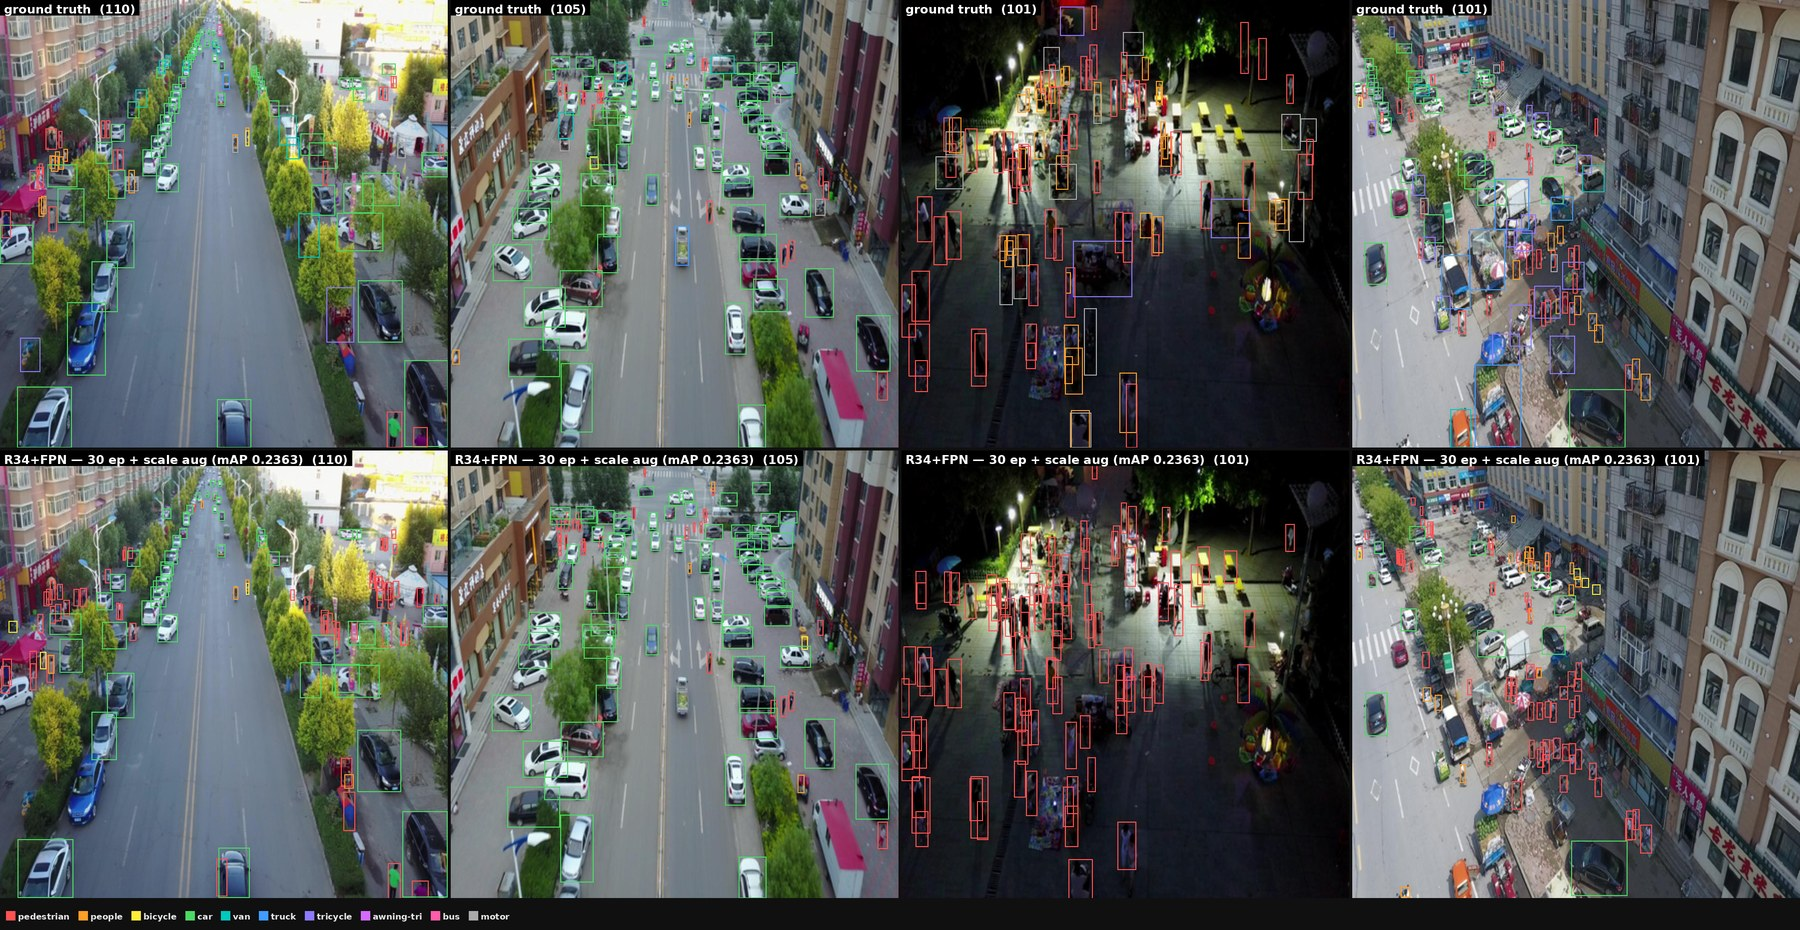
\includegraphics[width=\textwidth]{demos/visdrone_fpn.jpg}
\caption{The detector on four VisDrone validation frames at $448$: ground truth
above, the R34+FPN's boxes below --- the bold row of
Table~\ref{tab:visdrone_results} at its first seed, mAP@0.5 $0.2363$. Box
colour is the class, keyed along the bottom
edge, and each frame's box count sits in its corner. The night market and the
street market are where the misses live --- the small and the rare.}
\label{fig:visdrone_fpn}
\end{figure}

\noindent \textbf{Augmentation and schedule length are one decision, not two,
and the five R34+FPN rows only mean something together.} Quadrupling the
schedule with augmentation off costs $18\%$, $0.157$ to $0.129$ --- ordinary
overfitting on $6{,}471$ images --- and no checkpoint of the 50-epoch run
reaches the 12-epoch run's number: its best is $0.136$--$0.145$ at epoch 10 or
20, under the 12-epoch row's lowest seed, $0.153$, and every seed falls
$0.007$--$0.015$ from there to epoch 50. Photometric augmentation recovers it.
With HSV jitter and flip on, the 50-epoch run scores $0.170$ and is flat from
epoch 10 to 50 --- $0.163$--$0.181$ across checkpoints and seeds, the peak at a
different epoch on each seed, so the checkpoint noise is the size of any
trend --- and the 12-epoch run under the same pack is $0.161 \pm 0.032$, not
above it. That row's three seeds end at $0.196$, $0.135$ and $0.152$ from
$0.139$--$0.144$ at epoch 8; the last four epochs of the cosine tail decide
it, and what moves there is the ranking, not the recall --- recall is
$0.744$--$0.749$ on every seed from epoch 10 while class-agnostic AP goes to
$0.441$ on one seed and stays at $0.31$--$0.32$ on another, which nothing the
trainer prints can see. Augmentation that changes object scale is a different
tier: the 30-epoch scale-augmented row is $0.232 \pm 0.004$, and its curve
climbs to epoch 28--30. Without augmentation the long schedule is worse than
the short one at every checkpoint; with photometric augmentation it is flat;
with scale augmentation it pays. \textbf{The pack sets whether the long
schedule pays}, so there is no epoch count that can be tuned once and carried
across packs.\footnote{The bold row and the 12-epoch HSV+flip row train the
class term under focal loss with the class weights off; the other three
R34+FPN rows use the trainer's default square-root class weights without the
focal term. The 12-epoch HSV+flip row is the bold row's recipe without the
scale augmentation, at 12 epochs.}

\medskip\noindent \textbf{The mean hides where detection fails.} Per-class
AP on the bold row runs from car, $0.66$, down to bicycle, $0.036$, a spread
of $18\times$, and scale augmentation narrowed it from $24\times$ by lifting
exactly the classes that were worst. Against the 12-epoch HSV+flip row, three
seeds on each side, awning-tricycle gains $1.9\times$, tricycle $1.6\times$
and bicycle $1.5\times$, car $1.1\times$; the direction holds on every seed,
and the seed spread of the bold row lives in the big classes --- car moves
$0.066$ across seeds --- while the four rarest agree to $0.002$. That the fix
was data rather than objective is the substantive point.
Reweighting a loss toward rare classes buys their recall at the expense of
precision, and average precision charges for the trade; supplying the scales the
rare classes are missing raises both at once, which is what the recall and
class-agnostic AP columns move together to show. Detection on aerial imagery does
not degrade uniformly --- it collapses on whatever is simultaneously small
and rare, and an averaged mAP is precisely the statistic that hides it.

\medskip\noindent The stack matches the hand-written PyTorch replica of
this same architecture on the matched recipe and decode, $0.151 \pm 0.004$
against $0.1532$ at 12 epochs without augmentation under the argmax decode
(the multilabel decode the table prints adds $0.004$--$0.007$ to every row
without the focal term and $0.02$ to the row with it, on every seed, and
changes no ordering), and runs at 65\,fps on one RTX 4060 Ti
--- or $55.9$\,fps on a 25\,W Jetson Orin Nano under TensorRT, with a
uint8 input path and the clocks pinned. The replica, not YOLOv8, is the
yardstick: it
isolates implementation quality from architecture, which a comparison against a
different model would conflate. The two YOLOv8s rows say something more
interesting than either alone. At a matched budget it scores $0.140$ --- below
this detector, though from random weights rather than an ImageNet-pretrained
backbone --- while its ordinary-practice $0.391$ comes from $8\times$ the epochs,
higher resolution, full augmentation and COCO pretraining. \textbf{The distance
to the field is recipe, not architecture}, and one item of that recipe, scale
augmentation with the schedule it needs, closes $0.07$ of the $0.23$
between the matched 12-epoch row and the field.

\medskip\noindent What this detector is not: a tracker, or the field's
number. It reads one $448$-px frame --- no identity from frame to frame, no
count over a sequence, though the validation records are video --- and on the
classes that are small and rare at once the honest number is the per-class
one, bicycle at $0.036$, not the mean.

\subsection*{YOLO v1/v3/v5/v8/v11 (\texttt{Bestiary/YOLO.lean})}
v1 (Redmon et al.\ 2016,
\href{https://arxiv.org/abs/1506.02640}{arXiv:1506.02640}) uses
\emph{zero} new primitives (\texttt{conv2d} + \texttt{maxPool} +
\texttt{flatten} + \texttt{dense}; the YOLO-ness lives in the loss and
output reshape, not the architecture). v3 adds Definition~\ref{layer:darknetBlock}
for the Darknet-53 body. v5/v8/v11 use Definition~\ref{layer:cspBlock} for
their CSPDarknet backbones. Variants: YOLOv1 (271M, paper-exact; the first FC's fan-in is pinned to the
paper's $7 \cdot 7 \cdot 1024$, while the spec's own body ends at $28 \times 28$), fast,
tiny, YOLOv3 (40M backbone), YOLOv5s/m (3M/8M single-scale), YOLOv8n/s
(0.7M/2.9M single-scale), YOLOv11n/m (backbone only). The entries show a
single-scale view; the multi-scale head is the demo's \texttt{.fpnDetect}
(Definition~\ref{layer:fpnDetect}), which taps three backbone stages the
way \texttt{.unetUp} taps its skips.

\begin{verbatim}
def yolo : NetSpec where
  name   := "YOLOv1 (Redmon 2016)"
  imageH := 448
  imageW := 448
  layers := [
    .conv2d 3 64 7 .same .relu,
    .maxPool 2 2,
    .conv2d 64 192 3 .same .relu,
    .maxPool 2 2,
    -- Block 3: 1×1 reduce + 3×3 expand
    .conv2d 192 128 1 .same .relu,
    .conv2d 128 256 3 .same .relu,
    .conv2d 256 256 1 .same .relu,
    .conv2d 256 512 3 .same .relu,
    .maxPool 2 2,
    -- Block 4: four 1×1+3×3 pairs, then 1×1 + 3×3
    .conv2d 512 256 1 .same .relu, .conv2d 256 512 3 .same .relu,
    .conv2d 512 256 1 .same .relu, .conv2d 256 512 3 .same .relu,
    .conv2d 512 256 1 .same .relu, .conv2d 256 512 3 .same .relu,
    .conv2d 512 256 1 .same .relu, .conv2d 256 512 3 .same .relu,
    .conv2d 512 512 1 .same .relu,
    .conv2d 512 1024 3 .same .relu,
    .maxPool 2 2,
    -- Block 5: two 1×1+3×3 pairs + two more 3×3 convs
    .conv2d 1024 512 1 .same .relu, .conv2d 512 1024 3 .same .relu,
    .conv2d 1024 512 1 .same .relu, .conv2d 512 1024 3 .same .relu,
    .conv2d 1024 1024 3 .same .relu,
    .conv2d 1024 1024 3 .same .relu,
    -- Block 6: two 3×3 at 7×7
    .conv2d 1024 1024 3 .same .relu,
    .conv2d 1024 1024 3 .same .relu,
    -- Head: flatten + 2 FC → reshape to (7, 7, 2·5 + 20) = 1470
    .flatten,
    .dense (7 * 7 * 1024) 4096 .relu,
    .dense 4096 yoloHeadSize .identity   -- 7 * 7 * (2 * 5 + 20)
  ]
\end{verbatim}

\subsection*{Mask R-CNN (\texttt{Bestiary/MaskRCNN.lean})}
\emph{One} new primitive (Definition~\ref{layer:fpnModule}); the \texttt{.bottleneckBlock} backbone is built from the block Chapter~\ref{chap:residual} proves for ResNet-50, here at ResNet-101's depth. The canonical two-stage detector +
instance segmentation reference (He et al.\ 2017,
\href{https://arxiv.org/abs/1703.06870}{arXiv:1703.06870}). Five architectural
pieces: ResNet-FPN backbone, RPN for anchor-box proposals, ROI-Align
for per-proposal feature extraction (an orchestration step, not a
layer), a 2-layer FC box head for classification + bbox regression,
and a 4-conv + transposed-conv mask head for per-class $28 \times
28$ masks. Shown as separate NetSpecs per head (SAM-style
decomposition). Param totals: backbone+FPN 45.8M, box head 14.3M,
mask head 2.6M, RPN 0.6M --- $\sim$63M in total. The
FPN cross-scale add is the one thing that demanded a new bundled
primitive; everything else reuses existing ResNet / conv / dense
primitives. DETR is its end-to-end transformer-era cousin; Mask2Former
is the DETR-style instance-segmentation successor.

\begin{verbatim}
def maskRCNNBackboneR101 : NetSpec where
  name   := "Mask R-CNN backbone (ResNet-101-FPN)"
  imageH := 800
  imageW := 800
  layers := [
    -- ResNet-101 stem + body (C2..C5)
    .convBn 3 64 7 2 .same,
    .maxPool 3 2,
    .bottleneckBlock 64   256  3  1,            -- C2
    .bottleneckBlock 256  512  4  2,            -- C3
    .bottleneckBlock 512  1024 23 2,            -- C4
    .bottleneckBlock 1024 2048 3  2,            -- C5
    -- FPN: combines C2–C5 into a 4-level feature pyramid at 256 channels
    .fpnModule 256 512 1024 2048 256
  ]
\end{verbatim}

\subsection*{DETR (\texttt{Bestiary/DETR.lean})}
\emph{Two} new primitives (Definition~\ref{layer:transformerDecoder},
Definition~\ref{layer:detrHeads}; Carion et al.\ 2020,
\href{https://arxiv.org/abs/2005.12872}{arXiv:2005.12872}); reuses
existing \texttt{bottleneckBlock} (ResNet backbone),
\texttt{patchEmbed} (absorbs the DETR 1$\times$1 channel reduce), and
\texttt{transformerEncoder}. Variants: DETR-R50 (41M, paper-exact),
DETR-R101 (60M), tiny.

\begin{verbatim}
def detrR50 : NetSpec where
  name   := "DETR-R50"
  imageH := 800
  imageW := 800
  layers := [
    -- ResNet-50 backbone (stem + 4 stages)
    .convBn 3 64 7 2 .same,
    .maxPool 2 2,
    .bottleneckBlock 64 256 3 1,                -- C2
    .bottleneckBlock 256 512 4 2,               -- C3
    .bottleneckBlock 512 1024 6 2,              -- C4
    .bottleneckBlock 1024 2048 3 2,             -- C5
    -- Channel projection (2048→256) + flatten spatial + pos embed
    .patchEmbed 2048 256 1 625,                 -- 25×25 = 625 tokens
    .transformerEncoder 256 8 2048 6,           -- 6 encoder blocks, 8 heads
    .transformerDecoder 256 8 2048 6 100,       -- 6 decoder blocks, 100 queries
    .detrHeads 256 91                           -- class (→92) + box (→4)
  ]
\end{verbatim}

\section{Industrial inspection --- demo: the same detector on NEU-DET steel defects}
\label{sec:bestiary_inspection}

The detector of \S\ref{sec:bestiary_detection}, unchanged --- backbone,
neck, heads, loss, ImageNet bootstrap, scorer --- on the dataset the
industrial-inspection literature reports on.

\textbf{The data.} NEU-DET (Song \& Yan 2013; boxes He et al.\ 2020;
Appendix~\ref{app:data}) is
$1{,}800$ grayscale $200\times200$ crops of hot-rolled steel strip, $300$ per
class over six defect types --- crazing, inclusion, patches, pitted surface,
rolled-in scale, scratches --- with Pascal-VOC boxes. It is VisDrone's opposite
regime. A crop holds $2.3$ defects, half of which span more than half the frame;
at the detector's $448$\,px input, $98\%$ of the training boxes route to the
coarsest pyramid level and none to the finest. This is the dataset on which a
single $14\times14$ grid should not collapse, and running both heads on
both datasets is what shows when multi-scale detection pays.

Three constants change and nothing in the code generation does: the anchor
priors are re-fitted to NEU's boxes (VisDrone's largest is $0.18\times0.15$ of
the frame; a steel defect is often half of it), the class weights are off
(the data is balanced), and the six classes take ids $0$--$5$ of the ten-slot
one-hot, since the $5+10$ per-anchor width is baked into the \texttt{fpnDetect}
emitter and the scorer averages over the classes present. NEU-DET ships no
split; the one here is $1{,}080/360/360$, stratified $180/60/60$ per class from
a fixed seed. Epochs are chosen on the validation $360$ and the numbers in
Table~\ref{tab:neudet_results} are the test $360$ at that epoch, scored by the VisDrone protocol against
uncapped ground truth, three seeds an arm --- the seed sets the He
initialisation of whatever is not bootstrapped, the shuffle and the
augmentation draws --- printed as mean $\pm$ sd
(\texttt{demos/MainYolov1NeuDetFpn.lean},
\texttt{demos/MainYolov1NeuDet448.lean};
\texttt{runs/2026-09-17-neudet-fpn-run1/},
\texttt{runs/2026-10-27-neudet-seeds/}). The single-grid arm is the same ResNet-34 and the same
bootstrap under a one-grid YOLOv1 head at $448/14$, run for the same 30
epochs here (its VisDrone run was 12 epochs without the scale
augmentation). Table~\ref{tab:neudet_visdrone_heads} is the same two heads on
VisDrone, and Figure~\ref{fig:neudet_fpn} is both on one crop of each defect.

\begin{table}[H]
\centering
\caption{Detection on the NEU-DET test split: the R34+FPN arms and the single-grid head, mean $\pm$ sd over three seeds of the test score at each run's validation-peak epoch (\texttt{runs/2026-10-27-neudet-seeds/}), and published detectors.}
\label{tab:neudet_results}
\small
\begin{tabular}{l c c c}
\hline
NEU-DET test, 3 seeds & mAP@0.5 & recall & class-agnostic AP \\
\hline
\textbf{R34+FPN, the VisDrone recipe} & \textbf{0.632 $\pm$ 0.008} & 0.992 $\pm$ 0.001 & 0.640 $\pm$ 0.013 \\
R34+FPN, HSV jitter and flip off, affine kept & 0.646 $\pm$ 0.015 & 0.991 $\pm$ 0.004 & 0.659 $\pm$ 0.017 \\
R34+FPN, no ImageNet bootstrap & 0.562 $\pm$ 0.012 & 0.986 $\pm$ 0.001 & 0.567 $\pm$ 0.014 \\
\textbf{R34, single $14\times14$ grid} & \textbf{0.609 $\pm$ 0.018} & 0.923 $\pm$ 0.008 & 0.606 $\pm$ 0.027 \\
published stock detectors, $640$\,px, 300\,ep & 0.73--0.78 & --- & --- \\
published improved variants & $\approx 0.83$ & --- & --- \\
\hline
\end{tabular}
\end{table}

\begin{table}[H]
\centering
\caption{The same two detection heads on VisDrone validation: the R34+FPN row of Table~\ref{tab:visdrone_results}, three seeds; the single grid, one run (\texttt{runs/2026-09-17-neudet-fpn-run1/}).}
\label{tab:neudet_visdrone_heads}
\small
\begin{tabular}{l c c c}
\hline
VisDrone val, the same two heads & mAP@0.5 & recall & class-agnostic AP \\
\hline
\textbf{R34+FPN}, 30\,ep, HSV+flip+scale aug, 3 seeds & \textbf{0.232 $\pm$ 0.004} & 0.769 $\pm$ 0.000 & 0.482 $\pm$ 0.011 \\
\textbf{R34, single $14\times14$ grid}, 12\,ep, 1 run & \textbf{0.0391} & 0.184 & 0.107 \\
\hline
\end{tabular}
\end{table}

\begin{figure}[H]
\centering
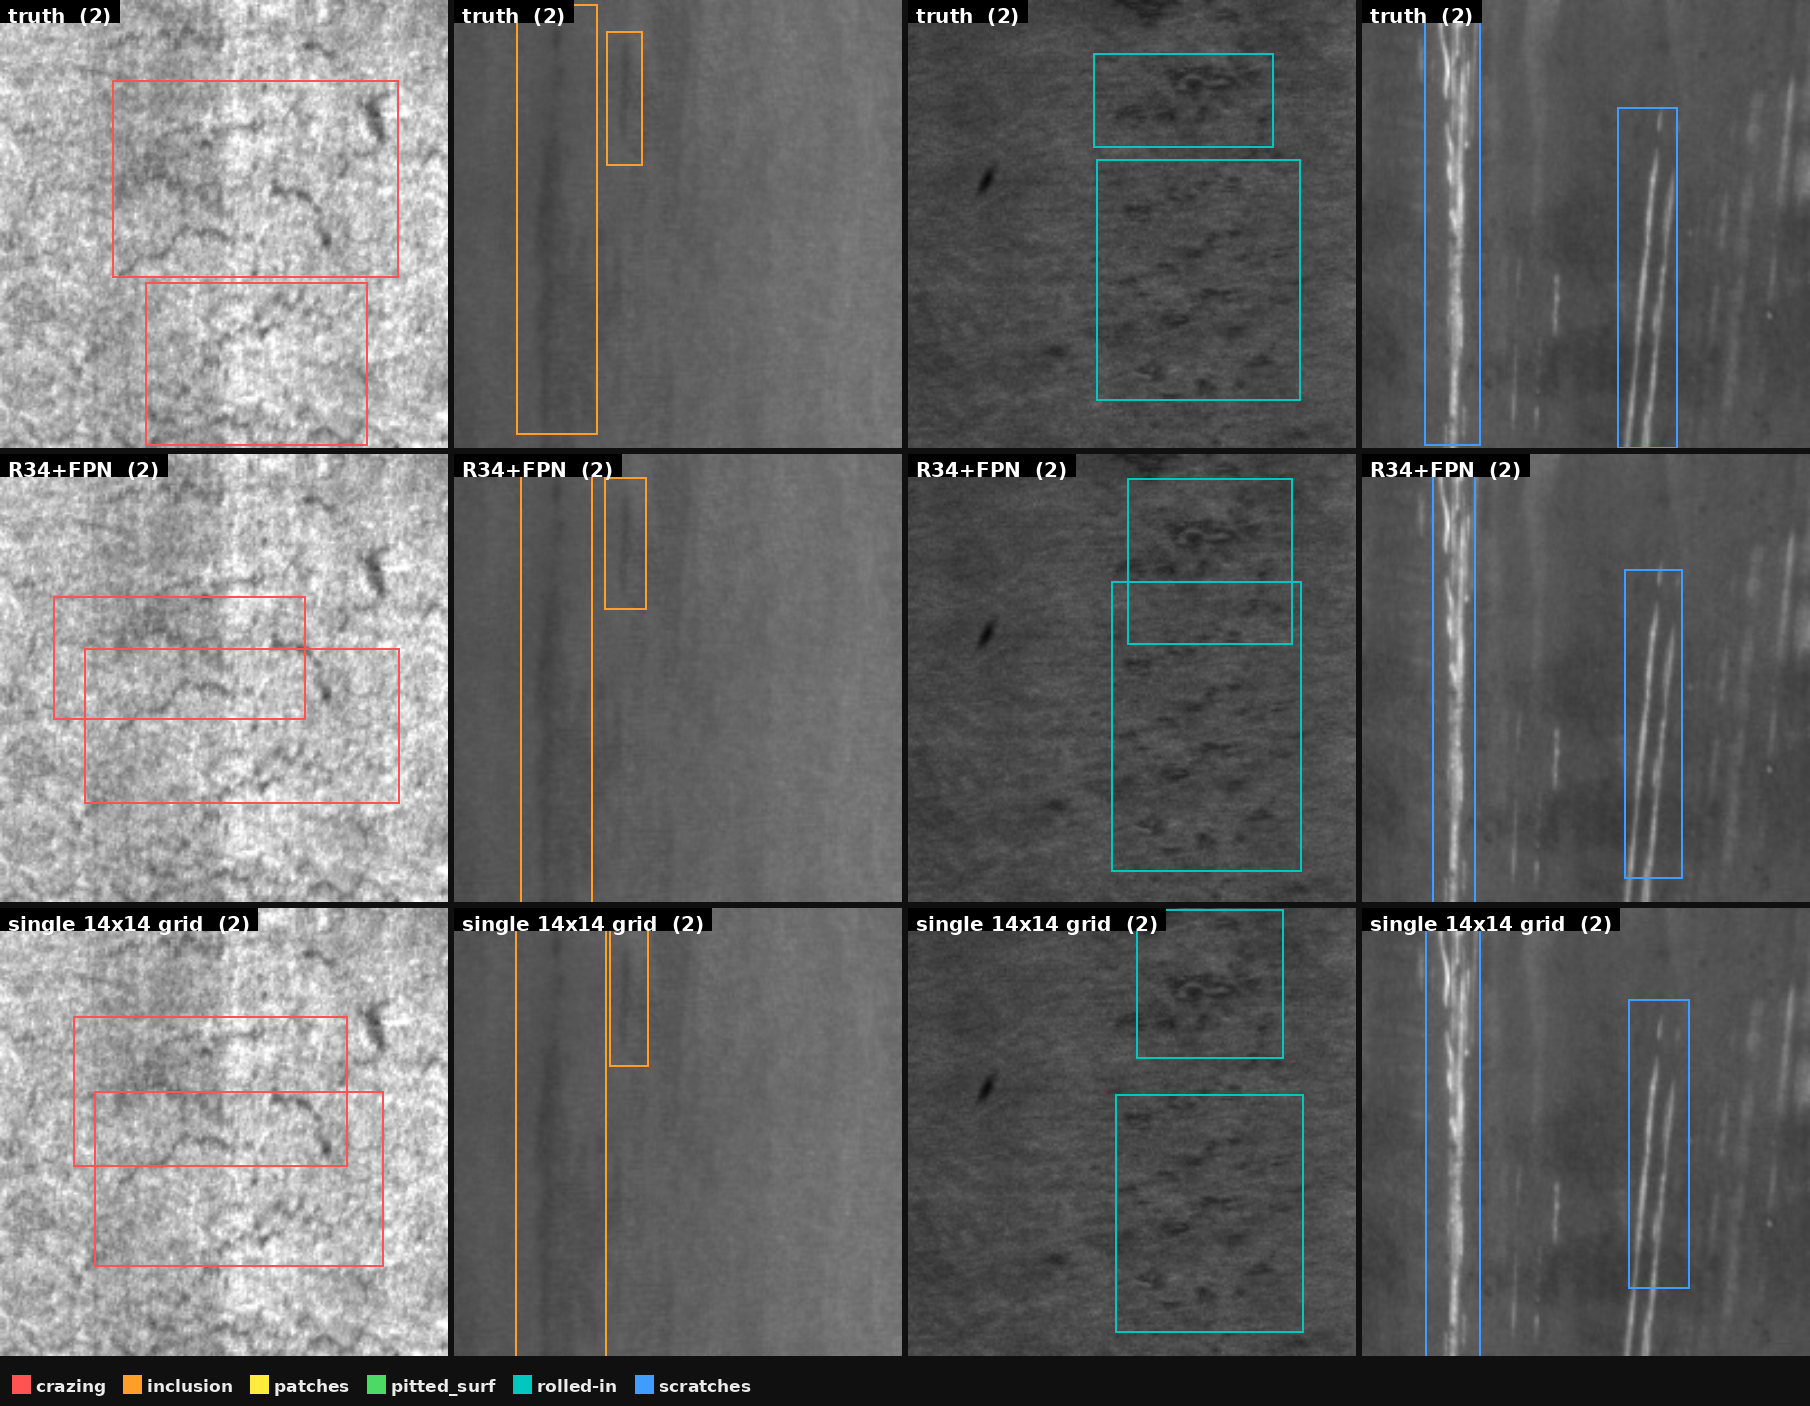
\includegraphics[width=\textwidth]{demos/neudet_fpn.png}
\caption{Truth (top), the R34+FPN (middle) and the single-grid head (bottom)
on one crazing, inclusion, rolled-in-scale and scratches crop from NEU-DET
validation, each with two ground-truth boxes; each model draws its two
highest-scoring boxes. Both heads find the same defects. Crazing, whose box
is a region of texture rather than an object, is where the boxes disagree
with the truth and with each other.}
\label{fig:neudet_fpn}
\end{figure}

\noindent \textbf{Table~\ref{tab:neudet_results} beside
Table~\ref{tab:neudet_visdrone_heads} is the result.} On steel the single
grid is within $0.02$ of the multi-scale head, $0.609$ against $0.632$ ---
behind on every seed, by $0.008$ to $0.044$; on drones it is six times
behind, $0.039$ against $0.232$, with recall $0.18$ against $0.77$ --- same
backbone, same bootstrap, same scorer, same lowerer in all four cells
(against the FPN's own 12-epoch unaugmented row, $0.157$, the grid is four
times behind). The FPN pays for itself only where objects are small; on
NEU-DET it runs three heads for one level's worth of work, and the head that
collapses on VisDrone is not wrong, it is wrong for drones. Recall is not the
limit on steel: the FPN finds $99\%$ of defects on every seed and the mean is
held down by two classes, crazing at $0.34$ and rolled-in scale at $0.43$
against $0.67$--$0.84$ for the other four --- the diffuse textures whose
``box'' is most of the crop, the worst two in every published NEU-DET table
and the worst two for every arm and seed here. The ImageNet prefix is worth
$0.071 \pm 0.011$ at $1{,}080$ training images, the same sign on all three
seeds and five times either arm's spread; without it the validation curve
sits $0.04$--$0.09$ lower at every epoch from 26. Switching the HSV jitter and
the flip off is $+0.014$, the same sign on all three seeds on test and on
validation, about one seed sd of the recipe arm: the crops are grey, hue
jitter on grey content is input noise, and the box-aware affine, kept in both
arms, is the augmentation doing the work. It is small, consistent, and not
the table's point; the bold row is the VisDrone recipe unchanged, and a
NEU-tuned recipe would start by switching the jitter off.

\medskip\noindent The distance to the published rows is recipe. Those
detectors run at $640$\,px for 300 epochs on a $1{,}440/180/180$ split; this
one runs at $448$\,px for 30 epochs, which on $1{,}080$ images is $4{,}050$
steps against VisDrone's $24{,}000$, under a cosine that has levelled by
epoch 26--30 on every arm and seed: the validation peak is epoch 28 or 30 on
eleven of the twelve runs, and the test score at epoch 30 is within $0.011$
of the score at the peak on all of them. The anchor priors are a second,
smaller part of it: three per level fit
a level that carries $98\%$ of the boxes at every aspect from $64$\,px to the
full frame at a mean IoU of $0.52$, and the head has to regress the rest.
Both are levers the detector already has; neither was pulled, because the
comparison the section makes needs the detector to be the detector.

\medskip\noindent What this detector is not: an inspection line. It draws a
box on a $200$-px crop already cut from the strip --- no line speed, no
severity, no miss rate against a plant's tolerance --- and on the two diffuse
classes, crazing at $0.33$--$0.35$ and rolled-in scale at $0.40$--$0.48$
across the four arms, the box is a region of texture that the labels, the
published detectors and both heads here place differently. The honest number
on steel is the per-class one.

\section{People watching --- demo: Arabic sign-language letters on ArASL}
\label{sec:bestiary_people}

Networks whose input is a person: a face, a gait, a hand. The demo is
Chapter~\ref{chap:bn}'s CIFAR net on the dataset the Arabic sign-language
literature reports on, run twice on the same images --- once under the
split every published number uses, once under a split that keeps each
hand's frames together --- and the pair of numbers is the result. ArASL
(Latif et al.\ 2019, Data in Brief~23; Mendeley \texttt{y7pckrw6z2}, CC~BY~4.0)
is $54{,}049$ grayscale $64\times64$ crops of static hand signs for the 32
letters of the Arabic alphabet, $1{,}293$ to $2{,}114$ per class, performed
by ``more than 40 people''. Published classifiers score $96.6$--$97.6\%$ for
CNNs trained from scratch (Latif et al.\ 2020; Alani \& Cosma 2021;
Abdelghfar et al.\ 2023) and $99.3$--$99.6\%$ for transfer-learned
EfficientNets and ViTs (Al Nabih et al.\ 2024; arXiv:2410.00681;
arXiv:2501.08169), all on random splits. The images are video bursts:
sorted by file number within a class, consecutive frames differ by a median
$3.3$ grey levels per pixel where a random pair of the same class differs by
$33$, and cutting where the gap exceeds $6$ leaves $14{,}336$ chains of $3.8$
frames. No signer, session or date is recorded. The two protocols are
$80/10/10$ per class from one seed: \texttt{random}, a stratified
permutation, and \texttt{blocked}, each class's capture order cut at the
$80\%$ and $90\%$ marks with each cut moved to the nearest chain boundary.
An audit then measures what the split did: for every test image, the
nearest training image of any class at $16\times16$. Under \texttt{random},
$92.3\%$ of test images have a training image within $6$ grey levels, and
the nearest training image's label is right $95.7\%$ of the time; under
\texttt{blocked}, $6.4\%$ and $28.6\%$. The residual $6\%$ is the same hand
returning a median $306$ files later, which a release without signer ids
cannot separate.

Two numbers change in the network and nothing in the code generation does.
\texttt{CIFAR-CNN8-wide-BN} as Chapter~\ref{chap:bn} spells it --- eight
convolutions in four conv-conv-pool stages at 16, 16, 32, 32 channels into
the $2\times512$ head --- takes a one-channel stem and a 32-way output; on
the native $64\times64$ input the four pools end at $4\times4$, so the
flatten is $512$ wide and the net is $0.58$\,M parameters. The recipe is the
one the gravitational-wave demo (\S\ref{sec:bestiary_signal}) also uses: the
ordinary train step with integer
labels, Adam at $10^{-3}$ with one warm-up epoch and cosine decay, batch 64,
30 epochs, no flip (a mirrored hand is a different sign for some letters),
five minutes on one card (\texttt{runs/2026-09-17-arasl/}, one directory per arm
beside it). The chapter's linear and MLP rungs run through
the same loop as the bracket, and the chapter net at its own $32\times32$
input checks that the resolution is not the story. Epochs are chosen on
the validation tenth and the numbers in Table~\ref{tab:arasl_results} are the
test tenth at that epoch, three seeds for the chapter net, with a $95\%$ Wilson interval on
the pooled $\approx 16{,}200$ trials of $\pm 0.2$ (random) and $\pm 0.6$ (blocked).
Figure~\ref{fig:arasl_signs} is the alphabet, the nearest neighbours under each
split, and the confusions.

\begin{table}[H]
\centering
\caption{ArASL test accuracy under a random and a blocked split.}
\label{tab:arasl_results}
\small
\begin{tabular}{l c c p{4.8cm}}
\hline
ArASL test, 80/10/10 per class & random split & blocked split & \\
\hline
\textbf{CIFAR-CNN8-wide-BN}, $64\times64$, 3 seeds & \textbf{98.62} $\pm$ 0.10 & \textbf{77.94} $\pm$ 0.80 & the demo \\
\quad with a near-duplicate in train & 99.73 & 98.46 & $92.3\%$ / $6.4\%$ of the test tenth \\
\quad without & 85.26 & 76.53 & $7.7\%$ / $93.6\%$ \\
CIFAR-CNN8-wide-BN at $32\times32$ & 98.21 & 71.03 & the chapter's own input \\
MLP $4096$-$512$-$512$-$32$ & 94.86 & 42.09 & what convolutions buy \\
linear $4096$-$32$ & 53.20 & 15.37 & the floor \\
1-NN on $16\times16$ thumbnails & 95.65 & 28.60 & nearest training image's label \\
published CNNs, from scratch & 96.6--97.6 & --- & 2020--23 \\
published transfer / transformer & 99.3--99.6 & --- & ViT, EfficientNet-B2, 2024--25 \\
\hline
\end{tabular}
\end{table}

\begin{figure}[H]
\centering
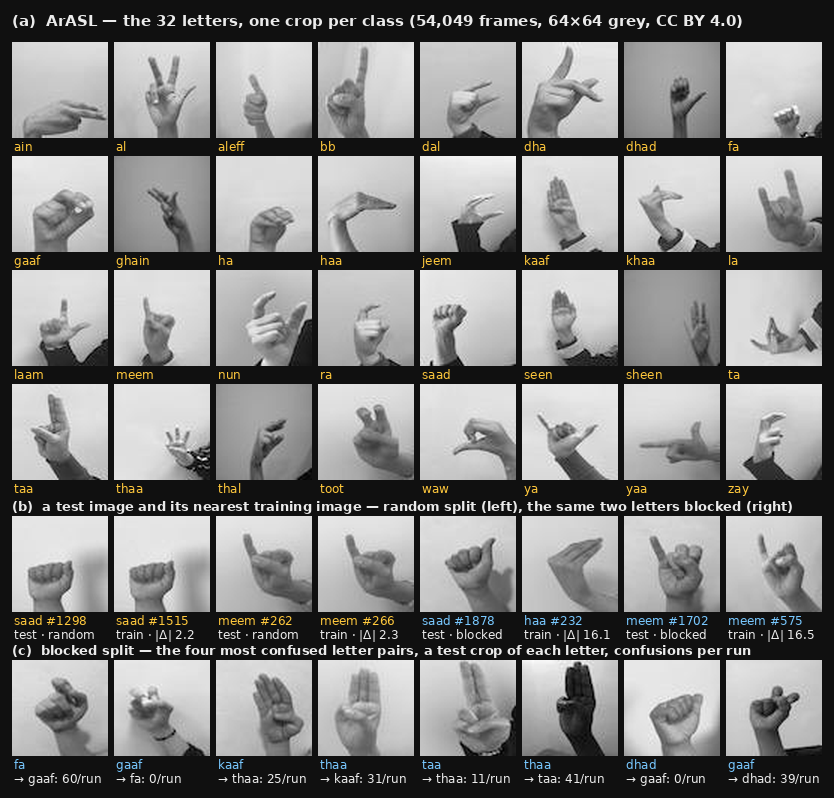
\includegraphics[width=\textwidth]{demos/arasl_signs.png}
\caption{(a) The 32 letters, one crop per class. (b) A test image and its
nearest training image for two letters, under the random split (left) and
the blocked split (right), with the mean grey-level gap per pixel: under
\texttt{random} the neighbour is the same hand two grey levels away; under
\texttt{blocked} it is a different hand sixteen levels away, and for
\emph{saad} a different letter. (c) The four most confused letter pairs on
the blocked split, a test crop of each letter and the count of each
confusion per run.}
\label{fig:arasl_signs}
\end{figure}

\noindent \textbf{The two columns are the result.} Under the literature's
protocol the chapter net scores $98.6\%$, above every published
from-scratch CNN and a point under the transfer-learned transformers; under
the blocked split the same net, recipe and seeds score $77.9\%$. The audit
says where the twenty points went. Nine in ten random-split test images
have a training image within six grey levels, and on those the net is at
$99.7\%$; on the $416$ that do not it is $85.3\%$; and a nearest-neighbour
lookup on $16\times16$ thumbnails --- no parameters, the training image's
label --- scores $95.7\%$ on the random split and $28.6\%$ on the blocked
one. The published $96$--$99\%$ is mostly the frame, not the hand. The
bracket says the same thing from below: the linear classifier loses $38$
points between the columns and the MLP $53$, because a pixel-space model
can only memorise the hand it saw, and the convolutions lose $21$, which is
the part of the letter they read. The chapter net at its own $32\times32$
input loses half a point on the random split and seven more on the blocked
one --- the difference between hands lives at a resolution the difference
between frames does not need. Per class, the blocked column runs from
$16.5\%$ (\emph{fa}) to $100\%$ (\emph{sheen}): the last tenth of some
classes' capture order is a hand no training frame covers, and the classes
farthest from their nearest training image are among the worst, but not
all the far ones fail --- \emph{al} and \emph{seen} sit as far from
training as \emph{fa} does and score $94\%$ and $100\%$. The rest is which
letter the new hand's shape lands near: \emph{fa} is called \emph{gaaf}
$181$ times in three runs and \emph{gaaf} is called \emph{fa} once, and
\emph{taa} and \emph{thaa}, which differ by one raised finger, confuse in
both directions.

\medskip\noindent Two caveats belong beside the number. The blocked split
is a proxy for a signer split, not one: the release records no signer, the
validation tenth sits next to the training tenths in capture order and is
$37.5\%$ leaked against the test tenth's $6.4\%$ (every blocked run shows
validation near $92\%$ and test near $78\%$, and the epoch is chosen on the
leakier of the two), and the $6\%$ of test hands that return from earlier
in the numbering is a floor the protocol cannot remove. And what this
classifier is not: it reads one static handshape per frame ---
fingerspelling, no motion, no grammar, no continuous signing --- and the
honest number for even that task on new hands is the right-hand column.

\section{Agriculture --- demo: lab leaves to field leaves on PlantVillage and PlantDoc}
\label{sec:bestiary_agriculture}

Networks that look at crops. The demo trains a leaf-disease classifier on
the dataset the agriculture literature uses most, reproduces its famous
number, and then asks the two questions that number does not answer: what
does the same net score on a photograph taken in a field, and what was it
looking at.

\textbf{The data.} PlantVillage (Hughes \& Salath\'e 2015; Mohanty, Hughes
\& Salath\'e 2016; CC~BY-SA~3.0) is $54{,}305$ photographs of single picked
leaves laid on a grey background in a laboratory: 38 classes over 14 crops
--- apple scab, tomato early blight, corn rust, grape black rot, and the
healthy leaf of each crop. Published classifiers score $99$--$99.7\%$ on a
random split of it. PlantDoc (Singh et al.\ 2020; CC~BY~4.0) is $2{,}578$
photographs of the same crops and diseases taken where they grow --- leaves
on the plant, several per frame, soil and sky behind them, phone lighting
--- in 28 classes that all map onto PlantVillage's; those are the counts of the
GitHub release \texttt{download\_plant.sh} fetches and checks, where the paper
reports $2{,}598$ in 27. The net here is
Chapter~\ref{chap:residual}'s ResNet-34 from its ImageNet weights with a
38-way head, ten epochs on PlantVillage, forty minutes on one card; PlantDoc
is never seen in training except by the three field-label rows of
Table~\ref{tab:plantvillage_results}, which
learn from it five-fold and are scored only on field images they did not
train on. (A near-duplicate audit of PlantVillage finds none, and the
maintainers' own leaf-grouped split gives the same number as a random one;
whatever the lab number hides, it is not a repeated frame.)

\begin{table}[H]
\centering
\caption{Accuracy on the PlantVillage test split and on the PlantDoc field photographs.}
\label{tab:plantvillage_results}
\small
\begin{tabular}{l c c p{3.9cm}}
\hline
& PlantVillage test & PlantDoc, all $2{,}578$ & \\
\hline
\textbf{ResNet-34, ImageNet prefix}, 3 seeds & \textbf{99.57} $\pm$ 0.06 & \textbf{17.80} $\pm$ 1.77 & the demo \\
\quad the same, random split & 99.72 & 16.56 & the papers' split \\
\quad the same, from scratch & 99.07 & 11.60 & what ImageNet buys \\
+ leaves on Imagenette backgrounds, 3 seeds & 99.44 $\pm$ 0.15 & \textbf{21.48} $\pm$ 1.25 & the diagnosis, attacked \\
+ photometric/geometric augmentation & 99.62 & 19.24 & the modern recipe \\
+ 250 field labels, five-fold & --- & 22.69 & ten per class \\
+ all field labels, five-fold & --- & 45.00 & $2{,}062$ per fold \\
+ backgrounds, then 250 / all field labels & --- & 26.57 / 42.05 & stack at few labels only \\
published, PlantVillage random split & 99.35 & --- & Mohanty et al.\ 2016 \\
published, on images from elsewhere & --- & $\approx 31$ & Mohanty et al.\ 2016 \\
\hline
\end{tabular}
\end{table}

\noindent \textbf{The first two columns are the result.} The net that
scores $99.6\%$ in the laboratory scores $18\%$ in the field ($2{,}578$
images, 28 classes, chance $3.6\%$). Nothing was wrong with the training;
the distribution was. The rest of the section asks the net what it learned,
with three instruments that need only the trained weights and the leaf mask
PlantVillage ships with every image. Table~\ref{tab:plantvillage_probes} is
what they find.

\begin{table}[H]
\centering
\caption{What the PlantVillage net responds to: edited test leaves and two explainers, for the base net and the net trained with backgrounds. The black-background cell is the one that moves with the seed; it lists the three seeds behind its mean.}
\label{tab:plantvillage_probes}
\small
\begin{tabular}{l c c}
\hline
What the trained net is asked, PlantVillage test ($10{,}709$) & base & + backgrounds \\
\hline
the test leaves as photographed & 99.6 & 99.4 \\
the same leaves on a black background & \textbf{60} (49, 59, 72) & \textbf{96} \\
the leaf on its own median background colour & 94 & 99 \\
the background only, leaf filled with that colour (chance 2.6) & \textbf{25} & 14 \\
a flat image of that colour and nothing else & 4.4 & 2.6 \\
\hline
Shapley value: share of the class evidence due to the leaf & 85\% & 96\% \\
Shapley value: images where the background helps & 88\% & 71\% \\
class-activation map: share of the map inside the leaf (uniform map: 59\%) & 71\% & 79\% \\
\hline
\end{tabular}
\end{table}

\noindent The upper rows are counterfactuals: the same test leaves, edited.
The lower rows are the two explainers. The class-activation map is the
usual heat map --- the class's weights applied to the last feature map ---
and the number is how much of its heat falls inside the leaf. The Shapley
value treats the image as a game with two players, the leaf and the
background, and asks how much of the class score each is responsible for;
with two players it is exact from four forward passes (the image, the leaf
alone, the background alone, neither), and the two shares add up to the
whole score. Both explainers say the same reassuring thing: the evidence is
mostly the leaf, $85\%$ of the Shapley share and $71\%$ of the map. The counterfactuals say otherwise. Put the same leaf
on black and the net loses forty points --- 28 to 51, by the seed; show it the background with the
leaf painted out and it is right one time in four; show it a flat rectangle
of the background's colour and it still beats chance. The background
helps in nine images out of ten, a little each time. A map of where
the evidence is heaviest does not say what the net cannot do without.
Figure~\ref{fig:plant_lab_to_field} is four test leaves under the maps, in the
laboratory and in the field.

\begin{figure}[H]
\centering
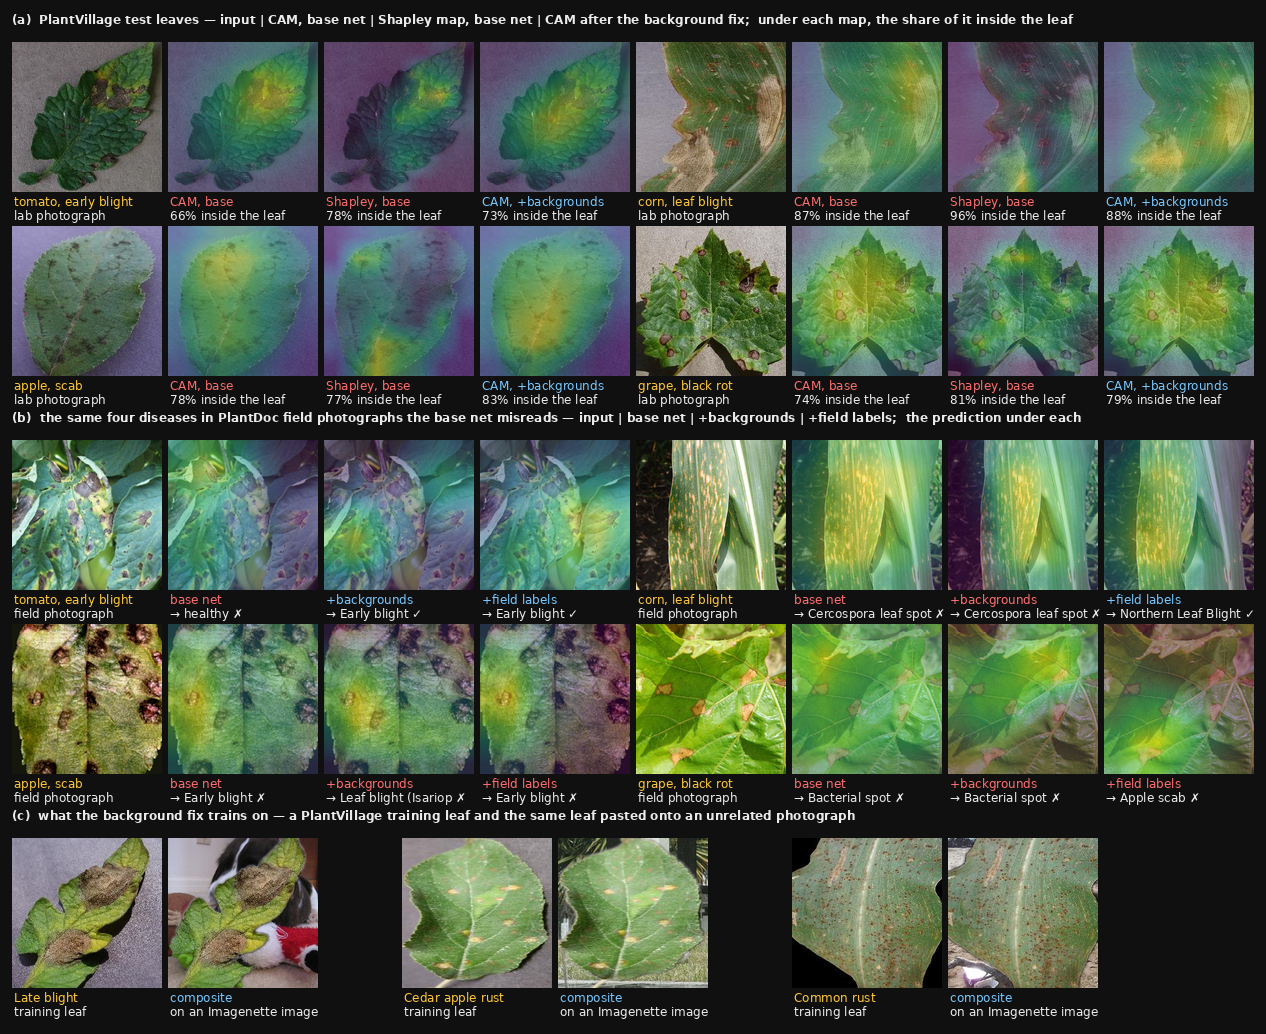
\includegraphics[width=\textwidth]{demos/plant_lab_to_field.png}
\caption{(a) Four PlantVillage test leaves --- tomato early blight, corn
leaf blight, apple scab, grape black rot --- with the class-activation map
and the Shapley map of the base net, and the map after the background fix;
under each map, the share of it inside the leaf. The heat is on the
lesions. (b) The same four diseases in PlantDoc field photographs the base
net misreads, with the map and the prediction of the base net, the
background-fixed net, and the net after field labels. (c) What the
background fix trains on: a training leaf and the same leaf pasted onto an
unrelated photograph.}
\label{fig:plant_lab_to_field}
\end{figure}

\noindent \textbf{The fixes.} Pasting every training leaf onto an unrelated
photograph (the composites of panel c) attacks exactly what the table
found, and repairs it: the leaves on black go from $60\%$ (49, 59 and 72 over three
seeds) to $96\%$, the
background alone falls toward chance, the leaf's Shapley share rises to
$96\%$. In the field it buys three and a half points, $17.8 \pm 1.8$ to
$21.5 \pm 1.3$ over three seeds each. Stronger augmentation --- colour,
rotation, erasing --- changes none of the diagnostics and stays inside the
seed noise. Field labels are what work: ten per class buy five points, all
two thousand buy twenty-seven, and the two fixes stack only while labels are
scarce. The laboratory artefact is real and removable, and removing it is
not what gets the net into the field.

\medskip\noindent What this classifier is not: a diagnosis. It reads one
leaf at one moment --- no severity, no spread across a field, no symptom
before the lesion shows --- and the honest number for even that, on a
photograph a grower would take, is the right-hand column.

\section{Remote sensing --- demo: which wavelengths travel, EuroSAT to the Amazon and the Cerrado}
\label{sec:bestiary_remote_sensing}

Networks that look down. The demo trains the Chapter~\ref{chap:bn} CNN on satellite
chips whose input is not a photograph --- thirteen bands of Sentinel-2,
ten of them outside what a camera sees --- five times, each time allowed a
different part of the spectrum, and then asks the trained nets, unchanged,
to read land they have never seen. Europe is a target that holds still.
The Amazon's arc of deforestation is a different place, and the Cerrado,
read in September and again in March, is a place that moves; the question
is which bands can follow it.

\textbf{The data.} EuroSAT (Helber et al.\ 2019; MIT) is $27{,}000$ chips
of Sentinel-2 imagery over 34 European countries, each $64\times64$ pixels
at 10~m --- a 640~m square --- in all 13 bands from 443 to 2190~nm, in ten
land-cover classes: annual crop, forest, herbaceous vegetation, highway,
industrial, pasture, permanent crop, residential, river, sea or lake. A
leaf is bright in the near infrared, where its spongy interior scatters
the light that chlorophyll absorbs in the red, and dark in the short-wave
infrared, where its water absorbs; the red edge is the step between the
two. Colour-infrared film found camouflage on that principle in the 1940s,
and the vegetation indices of the 1970s are ratios of exactly these bands.
The Brazil chips were cut for this section (Appendix~\ref{app:data}): the same 640~m
squares from Sentinel-2 scenes of 2023 over Rond\^onia between 16 June and
4 July, and over
western Bahia in September and again, the same $3{,}620$ squares, in
March, each labelled by majority vote from MapBiomas, Brazil's 10~m
land-cover map, through the seven classes EuroSAT's ten collapse into
(forest, pasture, herbaceous, annual crop, perennial crop, built, water).
The Cerrado's own class --- savanna, woody and herbaceous at once,
$2{,}000$ chips --- has no European name and is kept aside. The net is
Chapter~\ref{chap:bn}'s CIFAR CNN with the stem's input channels and, at
$64\times64$, the flatten width as the only changes: \texttt{rgb} (three bands), \texttt{rgbn} (plus near
infrared), \texttt{ms10} (the ten bands at 10 and 20~m), \texttt{all}
(thirteen), and \texttt{ir} (red edge, near and short-wave infrared, and
no visible light at all); 80 epochs with flips and rotations, three seeds,
five minutes an arm on one card. Nothing in the codegen moves.
Table~\ref{tab:eurosat_bands} is the five arms at home and abroad.

\begin{table}[H]
\centering
\caption{Accuracy by input bands, on EuroSAT test and on the Amazon and Cerrado windows.}
\label{tab:eurosat_bands}
\footnotesize
\setlength{\tabcolsep}{5pt}
\begin{tabular}{l c c c c c}
\hline
& EuroSAT & Amazon & Cerrado & Cerrado & same answer \\
& test & June & September & March & both seasons \\
\hline
\texttt{rgb}  & 97.1 $\pm$ 0.1 & 87.4 $\pm$ 0.9 & 33.2 $\pm$ 0.5 & 37.7 $\pm$ 0.3 & 38\% \\
\texttt{rgbn} & 98.0 $\pm$ 0.1 & 89.3 $\pm$ 1.4 & 34.6 $\pm$ 0.6 & 39.0 $\pm$ 0.5 & 41\% \\
\texttt{ms10} & 98.4 $\pm$ 0.1 & \textbf{97.0} $\pm$ 0.6 & 32.8 $\pm$ 2.3 & \textbf{59.2} $\pm$ 0.5 & 27\% \\
\texttt{all}  & 98.3 $\pm$ 0.1 & \textbf{97.0} $\pm$ 0.5 & 35.4 $\pm$ 2.5 & 53.8 $\pm$ 4.3 & 24\% \\
\texttt{ir}   & 97.9 $\pm$ 0.1 & 91.7 $\pm$ 1.5 & 29.0 $\pm$ 2.5 & 39.8 $\pm$ 3.1 & 39\% \\
\hline
trained in Brazil, five-fold & --- & \multicolumn{3}{c}{\texttt{rgb} 94.2 $\pm$ 0.7 \quad \texttt{all} 95.8 $\pm$ 0.6} & --- \\
Helber et al.\ 2019, ResNet-50 & 98.6 & --- & --- & --- & --- \\
\hline
\end{tabular}
\end{table}

\noindent \textbf{The first column is the literature's question and the
second is the demo's.} In Europe the ten invisible bands are worth about a
point to a small net trained from scratch, and the bands a camera cannot
see are enough on their own (\texttt{ir}, 97.9); the published ordering
--- RGB 98.6, colour-infrared 98.3, short-wave infrared 97.1 --- was the
ImageNet pretraining, not the spectrum. In the Amazon the
same bands are worth ten. Rond\^onia is forest and pasture; every arm finds
the forest ($99.8\%$ of it), and RGB loses a quarter of the pasture ($74\%$
recall) where the ten-band arm keeps $95\%$. Near infrared alone buys two
of the ten points and the red edge and short-wave infrared buy the other
eight;
the arm with no visible light at all reads 91.7.

\textbf{The Cerrado is the harder question, twice.} In September every arm
falls to a third, and the confusion is one line of the matrix: a paddock in
the dry season is ``herbaceous vegetation'' to a net that learned pasture
from European meadows (RGB puts 666 of 884 there), and the biome's own
class, savanna, is ``herbaceous'' to all five arms. Merge herbaceous and
pasture into one grass class and RGB reads 76; the multispectral arms 65 to
73, because they also send a share of the dry paddocks to ``annual crop''
--- bare, dry ground is a ploughed field in the short-wave infrared. In
March the same chips are green, the ten-band arm reads 59 and RGB 38, and
savanna becomes ``forest'' to RGB on $42\%$ of its chips. The last column
is the check the section was built for, and it fails for every arm: the
same $3{,}620$ chips get the same answer in the two seasons between a
quarter and two-fifths of the time. The multispectral arms are better in
both seasons; they are not stabler. Averaged over the Cerrado chips, red
and the second short-wave band are $1.9$ times as bright in September as in
March, the first short-wave band $1.5$ times, and the near infrared is
darker; no European chip taught that.

\textbf{Whose fault.} Trained on the Brazil labels themselves, five-fold,
the same net reads $94.2$ with three bands and $95.8$ with thirteen: the
labels are learnable, and the thirteen-band margin over RGB is the same
point and a half as in Europe. Fine-tuned from the European weights on 300
Brazilian labels, three arms were tried: \texttt{rgb} reaches $90.0$,
\texttt{ir} $89.2$ and \texttt{all} $91.0$. Fine-tuned on all the labels
they reach $94.3$, $94.9$ and $95.1$, which for the two with a from-scratch
row is within a point of it: the European start is worth nothing over
scratch. A five-player Shapley value over band groups --- visible, red edge,
near infrared, short-wave infrared, and the three atmospheric bands at
60~m; a removed group set to its training mean, exact over 32 forward
passes per chip --- says where the thirteen-band net's evidence came from:
a third of it from visible light on either continent, the short-wave share
rising from $13\%$ at home to $22\%$ abroad, and the atmospheric bands
worth less than nothing in Brazil ($-3.0$ nats of log-probability in the
Amazon). They had learned Europe's sky, which is why the arm without them gives
up nothing: \texttt{ms10} ties \texttt{all} in the Amazon and leads it in
March. Figure~\ref{fig:remote_sensing_wavelengths} is three of the
Brazilian windows under three of the arms.

\begin{figure}[H]
\centering
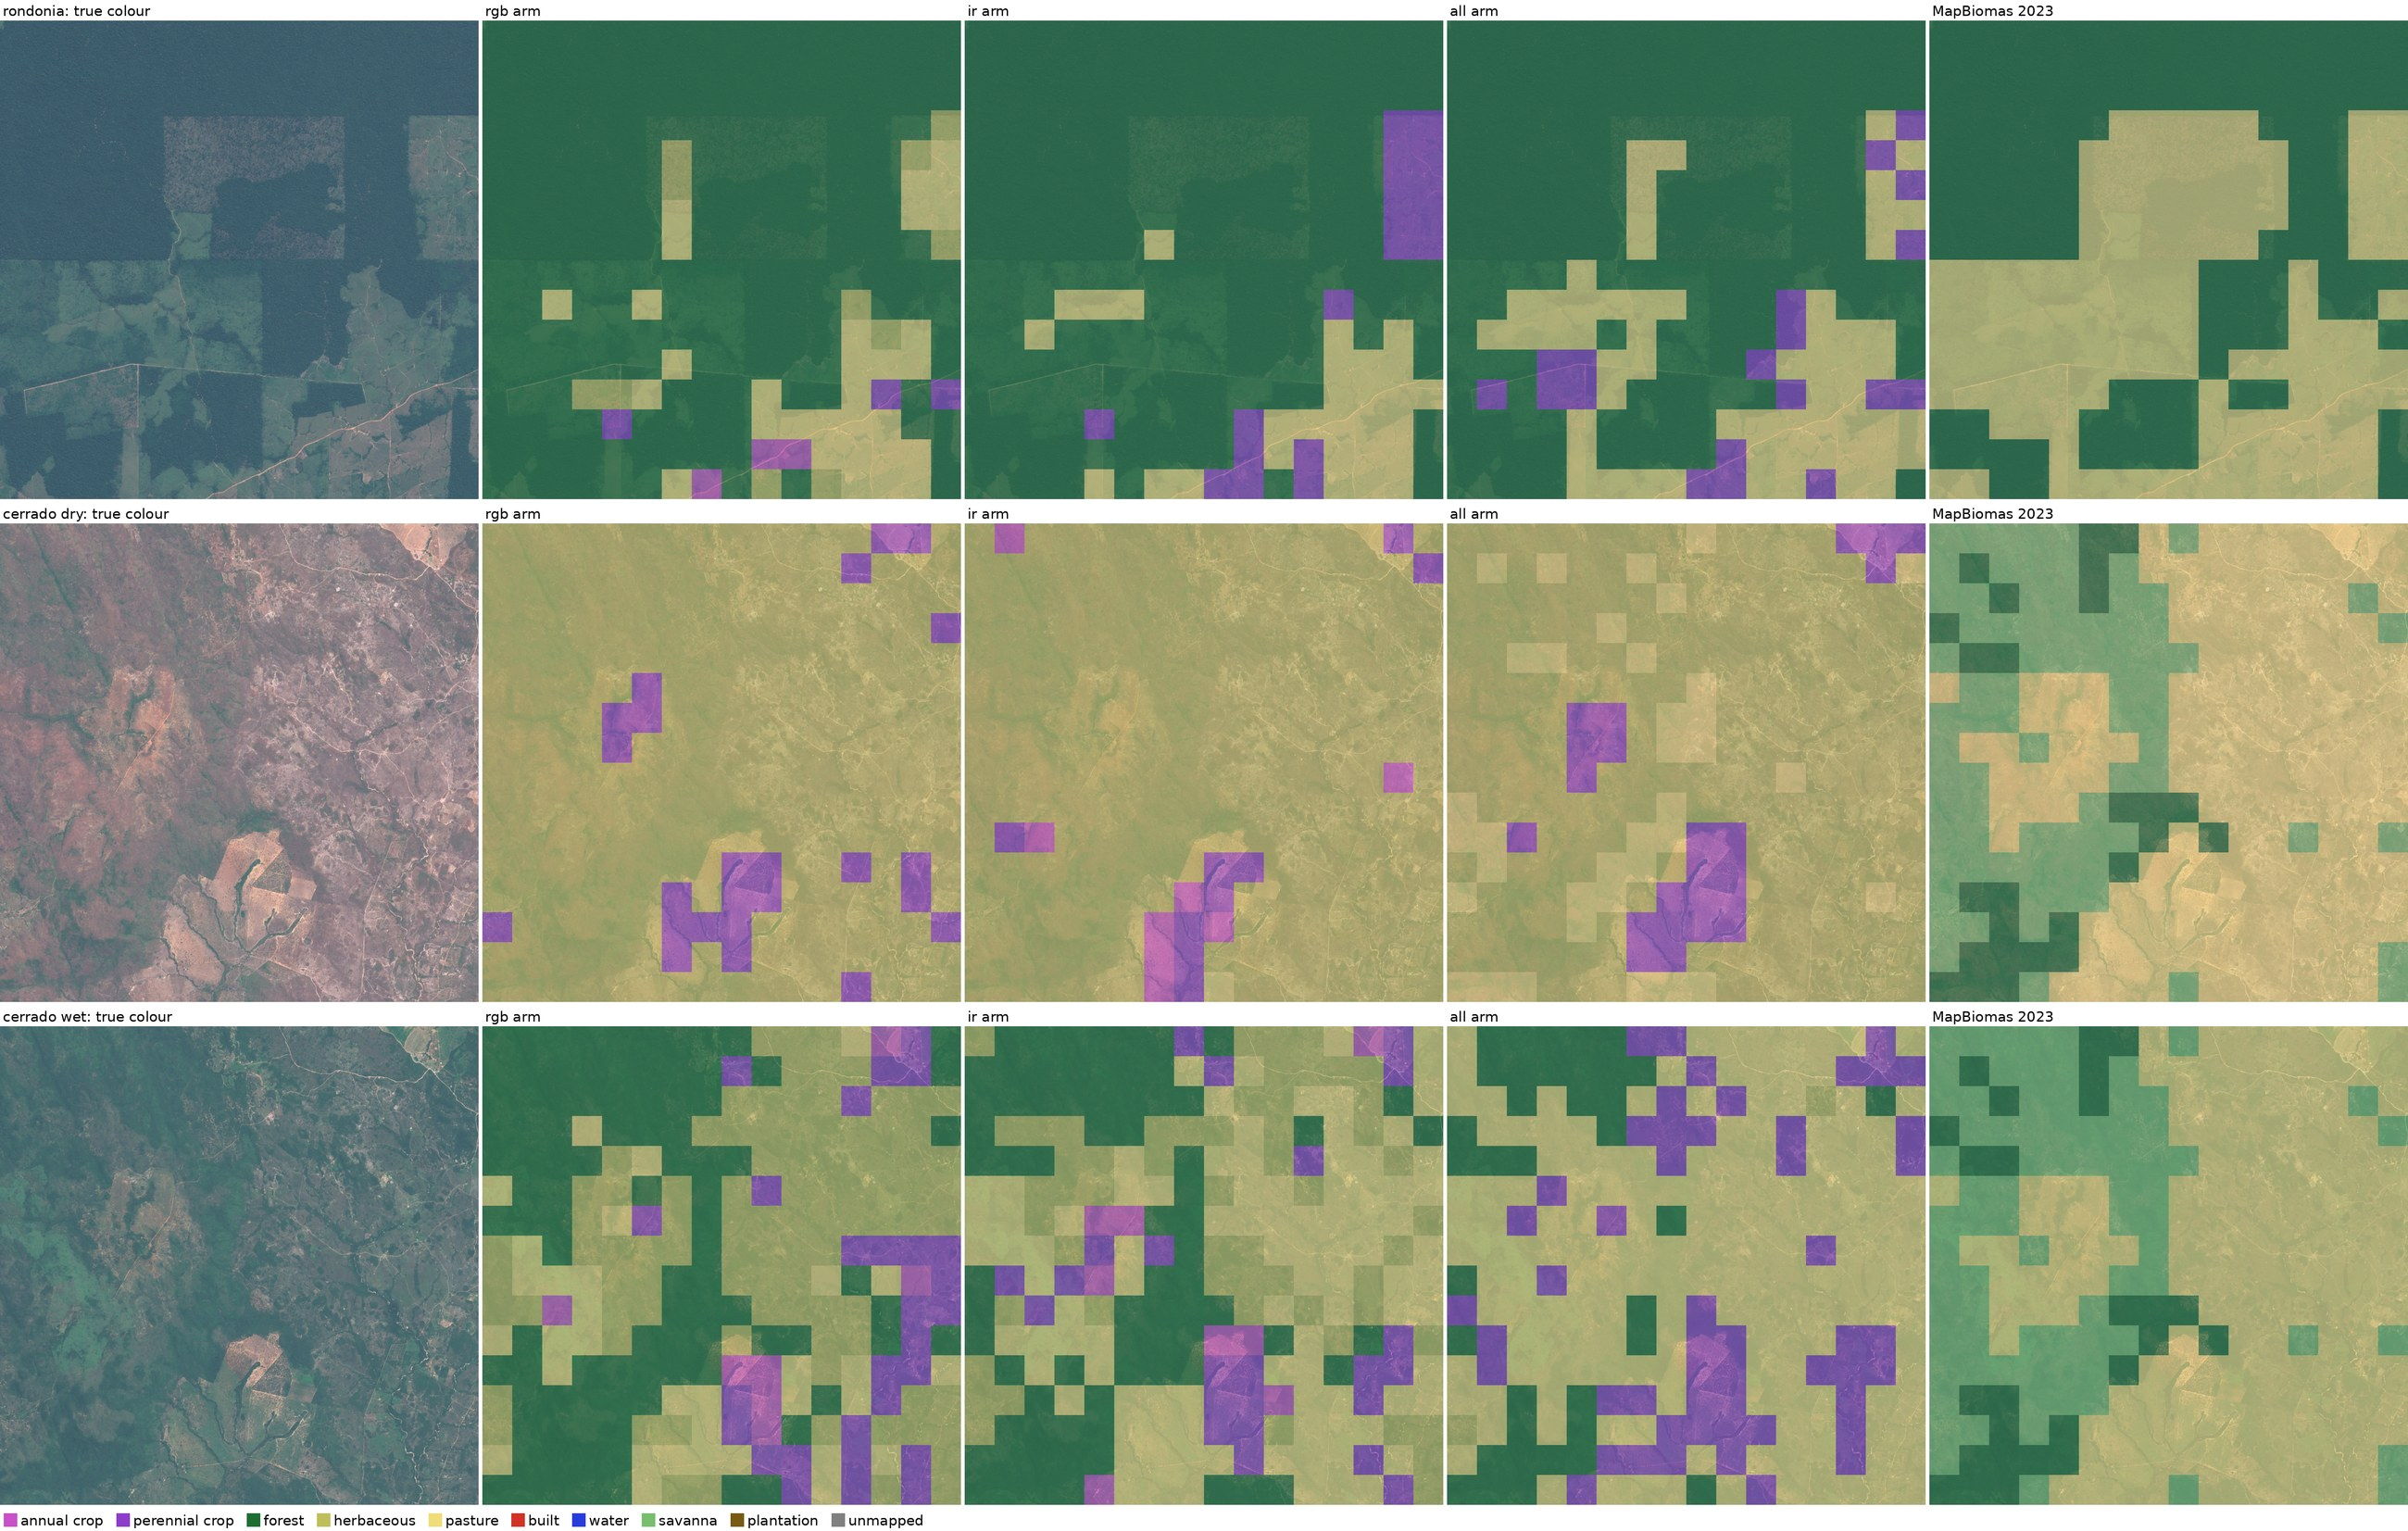
\includegraphics[width=\textwidth]{demos/remote_sensing_wavelengths.jpg}
\caption{Three 10~km windows, each a row: Rond\^onia in June, western
Bahia in September, and the same Bahia window in March. Left, the scene in
true colour; then the grid of 256 chips of 640~m coloured by what the
\texttt{rgb}, \texttt{ir} and \texttt{all} arms call each one, blended over
the scene; right, MapBiomas 2023. In the first row the clearings between
the forest ribs are pasture on the map, mostly ``herbaceous'' to RGB, and
pasture to the thirteen-band arm. In the second and third rows the map does
not change between the seasons and every column of predictions does: RGB
turns a third of the window to ``forest'' in March.}
\label{fig:remote_sensing_wavelengths}
\end{figure}

\noindent What travelled was the physics: the bands where a leaf's
structure and water are, which read the same over a Bavarian spruce stand
and a Rond\^onia pasture, and carried a net trained on one to the other
with no loss worth mentioning. What did not travel was the vocabulary. A
class list written for one continent has no word for the other's biome and
a different word for its grass, and the season that turns that grass brown
turns every one of these nets around with it. The first is a reason to keep
the invisible bands; the second is a reason to label where you look.

\medskip\noindent What this classifier is not: a map. It says what a 640~m
square mostly is --- not where the boundary runs, when the forest was cut,
or how much of it is gone.

\section{Semantic segmentation --- demo: UNet on BraTS}
\label{sec:bestiary_segmentation}

Pixel-level labeling. Symmetric encoder/decoder with skip connections
is the recurring pattern; UNet is the canonical instance, and the same
shape later became the diffusion-model backbone.

\paragraph{A ResNet-34 UNet on BraTS.} The question is what a slice
segmenter built from the Part~1 kit scores on brain-tumour MRI, and what its
two borrowed parts --- the ImageNet encoder and the decoder's skip
connections --- are each worth. The
\texttt{demos/MainUnetBratsR34.lean} trainer (\texttt{unet-brats-r34}) is an
encoder--decoder segmentation network at 24.5M parameters on MSD Task01
brain-tumour MRI: four co-registered modalities (FLAIR / T1w / T1gd / T2w) at
$224 \times 224$ in, four per-pixel classes out (background, edema,
non-enhancing/necrotic core, enhancing tumour), 14{,}415 training slices from
411 patients with the 2{,}569 validation slices held out by patient. The
tumour sub-regions are defined by which modality lights up --- edema is bright
on FLAIR, enhancing tumour on T1gd --- so the input is multi-modal rather
than three correlated views of one scene, and the classes are imbalanced:
enhancing tumour is about $0.5\%$ of voxels.

Scored on the clinical literature's regions --- Dice over the nested WT (whole
tumour), TC (tumour core) and ET (enhancing tumour) --- pooled over the 2{,}569
tumour-bearing validation slices, ten epochs of plain per-pixel cross-entropy
gives Table~\ref{tab:brats_dice}: three seeds an arm at each seed's
best-by-val epoch, about an hour an arm on one card, the encoder's ImageNet weights (the bootstrap the
detection sections also use) against the same encoder from He initialisation
(\texttt{runs/2026-09-25-brats-r34-xla/} for seed 0,
\texttt{runs/2026-10-27-brats-r34-seeds/} for seeds 1 and 2):

\begin{table}[H]
\centering
\caption{The ResNet-34 UNet on BraTS validation: mIoU, and Dice on the three tumour regions, pooled over the tumour-bearing slices. Ten epochs, batch 16 at $224^2$; mean $\pm$ sd over seeds 0, 1, 2 at each seed's best-by-val epoch, and the paired difference seed by seed.}
\label{tab:brats_dice}
\footnotesize
\setlength{\tabcolsep}{4pt}
\begin{tabular}{lcccc}
\hline
 & mIoU & WT & TC & ET \\
\hline
ImageNet bootstrap (\texttt{r34}), 3 seeds & $0.741 \pm 0.002$ & $0.912 \pm 0.001$ & $0.867 \pm 0.004$ & $0.856 \pm 0.003$ \\
from scratch (\texttt{scratch}), 3 seeds   & $0.737 \pm 0.004$ & $0.909 \pm 0.002$ & $0.864 \pm 0.005$ & $0.855 \pm 0.001$ \\
\quad paired, seeds 0/1/2 & $+.002/{+}.004/{+}.005$ & $+.003/{+}.002/{+}.005$ & $+.003/{+}.004/{+}.004$ & $-.000/{-}.001/{+}.003$ \\
\hline
\end{tabular}
\end{table}

\noindent The bootstrap is a small gain with the same sign on every seed:
$+0.004$ mIoU on average, WT and TC the same size, nothing on ET. It is the
size of one arm's own seed spread, so three seeds put it at the edge of what
they resolve; it is not a tie and it is not a rescue. At epoch 1 the arms are
level --- the ET gap is $+0.064$, $-0.035$ and $-0.003$ over the three seeds,
and both arms reach every 50 / 80 / 90\% target within one epoch of each
other --- so at 14{,}415 slices the pretrained encoder buys the last few
thousandths, not the first epoch. Seed 2 is the rough seed on both arms: its
validation mIoU drops $0.04$--$0.06$ between epochs 1 and 2 under either
initialisation, so the dips come from the shuffle and augmentation draws, not
the weights, and a single best-by-val row carries about $0.005$ of noise of
its own.

\noindent Rendered predictions are Figure~\ref{fig:brats_unet} --- T1gd
backdrop, ground truth, prediction, on four held-out patients. This matters more
than the table for a segmentation demo: a model that has collapsed onto the
majority class and one that works report similar pixel accuracy, because 97\% of
voxels are background. They do not produce similar pictures.

\begin{figure}[H]
\centering
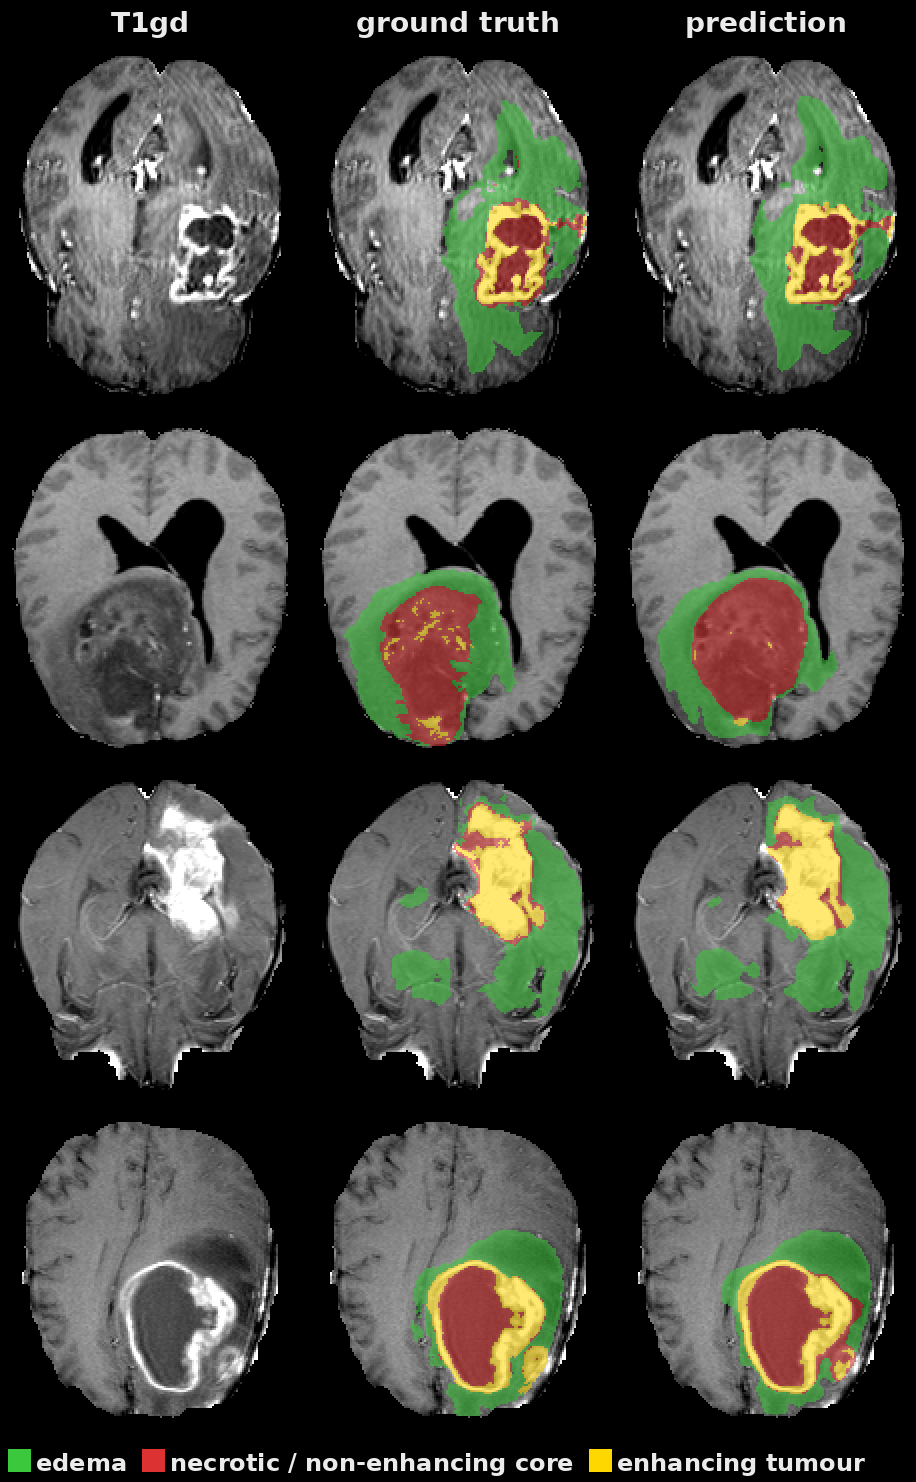
\includegraphics[width=0.52\textwidth]{demos/brats_r34_unet.png}
\caption{The ResNet-34 UNet on four held-out BraTS patients, one per row: the
T1gd slice, the ground truth, the prediction. Green is the edema that bounds the
whole tumour, red the necrotic and non-enhancing core, yellow the enhancing
tumour. Background is $97\%$ of the voxels, which is why this picture carries
more than the pixel accuracy does.}
\label{fig:brats_unet}
\end{figure}

The encoder is the ResNet-34 of Ch~\ref{chap:residual}, reused verbatim as the
contracting path rather than a stack of \texttt{.unetDown}s; the decoder is
four \texttt{.unetUp} stages, and the skips come off the backbone. The two
codegen primitives this rests on --- bilinear upsample (forward + VJP) and
channel concat --- are exposed at the \texttt{Layer} level as
\texttt{.unetDown} and \texttt{.unetUp}, which the catalogue UNet of this
section also uses. Three things change relative to the image
classifiers of Part~1:

\begin{itemize}
  \item \textbf{The label is a tensor, not a scalar.} A classifier emits
    one logit vector per image ($B \times K$) against one class. A
    segmentation network emits one per pixel ($B \times K \times H \times
    W$, $H \times W$ the input's) against a mask of the same shape, and the
    cross-entropy is per pixel, averaged over the plane. It is the
    per-position loss (\texttt{useSeg}, derived from the config's
    \texttt{lossKind}) the TinyGPT demo of \S\ref{sec:bestiary_nlp} applies
    per token, applied over the spatial axes instead: the per-pixel
    softmax-CE backward is the one Ch~\ref{chap:tensor} derived, fired $HW$
    times in parallel. No new VJP.
  \item \textbf{The network gives spatial resolution back.} A classifier
    downsamples on purpose, $224^2$ to a $7^2$ bottleneck to a pooled
    $K$-way vector. A segmentation network downsamples and then upsamples,
    with a skip from each encoder stage spliced into the matching decoder
    stage so the output recovers the detail the bottleneck discarded.
    \texttt{.unetUp} bundles that step --- bilinear upsample, channel concat
    with the saved skip, two convolutions --- and it is the only
    architectural piece this section adds to the Part~1 kit.
  \item \textbf{Inference is one forward pass; the post-processing
    differs.} One call produces every pixel's logits; \texttt{argmax} per
    pixel and a colormap make the mask. \texttt{brats-predict} is that path
    and nothing else: the trainer's artifact plus a colormap routine.
\end{itemize}

\paragraph{What the skips are worth, measured.} The second bullet is the
one claim in this section that is cheap to test. The same backbone, data and
schedule with the decoder's skip connections removed --- upsample and
convolve, never concatenate the encoder feature --- isolates what they
contribute, Table~\ref{tab:brats_skips}, three seeds a side:

\begin{table}[H]
\centering
\caption{The UNet decoder with and without its skip connections: the from-scratch arm, mean $\pm$ sd over three seeds at each seed's best-by-val epoch, and the paired difference seed by seed (\texttt{runs/2026-09-25-brats-r34-xla/}, \texttt{runs/2026-10-27-brats-r34-seeds/}).}
\label{tab:brats_skips}
\footnotesize
\setlength{\tabcolsep}{4pt}
\begin{tabular}{lcccc}
\hline
decoder & mIoU & WT & TC & ET \\
\hline
upsample only (no skips), 3 seeds & $0.634 \pm 0.003$ & $0.871 \pm 0.001$ & $0.816 \pm 0.003$ & $0.731 \pm 0.003$ \\
\texttt{.unetUp} (skips), 3 seeds & $\mathbf{0.737 \pm 0.004}$ & $\mathbf{0.909 \pm 0.002}$ & $\mathbf{0.864 \pm 0.005}$ & $\mathbf{0.855 \pm 0.001}$ \\
\quad paired, seeds 0/1/2 & $+.108/{+}.099/{+}.102$ & $+.039/{+}.039/{+}.036$ & $+.053/{+}.048/{+}.042$ & $+.123/{+}.122/{+}.128$ \\
\hline
\end{tabular}
\end{table}

\noindent Ten points of mIoU, $+0.103 \pm 0.005$, and the largest single gain
is on ET ($+0.124 \pm 0.003$), the smallest and thinnest structure --- which
is what the bullet predicts, since a decoder without skips must reconstruct
every boundary from a $7 \times 7$ bottleneck. The skipless arm's best epoch
is its last on every seed; it is still improving when the schedule ends. It
is visible in the renders as well: the thin enhancing rim around the necrotic
core is resolved with skips and smeared into the core without them.

\paragraph{Scored per patient.} Tables~\ref{tab:brats_dice} and
\ref{tab:brats_skips} pool every pixel of every
tumour-bearing slice into one Dice. The literature does something else: one
Dice per patient volume, over all of its slices including the tumour-free
ones, then the mean over patients --- so a small tumour counts as much as a
large one, and the slices where there is nothing to paint count against a model
that paints anyway. \texttt{brats-eval} (\texttt{demos/MainBratsEval.lean})
computes that from a whole-volume export of the 73 validation patients
(\texttt{preprocess\_brats.py --val-full}), and first re-derives the pooled
number on the same slices, where it agrees with the trainer's log line to
$0.0004$. Table~\ref{tab:brats_per_patient} is the seed-0 best-by-val
checkpoints:

\begin{table}[H]
\centering
\caption{Per-patient Dice on BraTS validation: the mean, with the median in parentheses. Seed 0 of each arm (\texttt{runs/2026-09-29-brats-25d/} for the slice models, \texttt{runs/2026-10-03-brats-3d/} for the 3D UNet).}
\label{tab:brats_per_patient}
\begin{tabular}{lccc}
\hline
per-patient mean Dice (median) & WT & TC & ET \\
\hline
ResNet-34 UNet, ImageNet bootstrap & 0.893 (0.914) & 0.821 (0.867) & 0.790 (0.858) \\
ResNet-34 UNet, from scratch       & 0.889 (0.917) & 0.819 (0.869) & 0.783 (0.851) \\
\quad without skips               & 0.843 (0.873) & 0.749 (0.801) & 0.620 (0.679) \\
from-scratch UNet $240^2$, Dice+CE, 3 ep & 0.882 (0.908) & 0.802 (0.850) & 0.782 (0.839) \\
\hline
ResNet-34 UNet, 2.5D ($\pm 1$ slice) & 0.893 (0.916) & 0.824 (0.868) & 0.788 (0.850) \\
3D UNet, $128^3$ patches, 20k steps (JAX) & 0.900 (0.918) & 0.827 (0.868) & 0.808 (0.867) \\
\hline
\end{tabular}
\end{table}

\noindent Two things the pooled number hid. The tumour-free slices cost almost
nothing: pooled over every slice the Dice is within $0.003$ of the tumour-slice
value, so the slice model does not paint tumour where there is none. And the
per-patient mean sits two to seven points below the pooled number with a wide
spread (standard deviations of $0.07$ on WT to $0.19$ on ET): the medians are
at the pooled values, and the means are pulled down by a tail of small-tumour
patients --- which is what the per-patient protocol exists to expose. The skips
are worth more per patient than per pixel, $+0.16$ on ET against $+0.12$. These
are the numbers scored the way published BraTS work scores, and they are
still not comparable to its tables: the 484-case MSD Task01 is not the
1{,}251-case BraTS~2021 set, and the split is this book's own.

\paragraph{Through-plane context.} A slice model never sees the slice above or
below. The last two rows measure what that costs, two ways. \texttt{unet-brats-r34
ctx=1} is the same net with the two neighbouring slices fed in as eight extra
input channels (a 2.5D build from \texttt{preprocess\_brats.py --context 1};
the stem is the only tensor that changes, and the records, their order, the seed
and the schedule are the 2D run's): it ties the 2D anchor within $0.005$ on every
metric, pooled and per patient. At 1~mm spacing the neighbours are nearly the
centre slice again, so this says adjacent slices add nothing the slice model
cannot infer, not that volumetric context is useless. The direct test is a 3D
UNet --- the from-scratch \texttt{unetBrats} of the table with $3^3$ kernels
and $2^3$ pools, 23.5M parameters --- trained in JAX on random $128^3$ patches for 20{,}000 steps,
a little over five hours on one card (\texttt{jax/scripts/unet3d\_brats.py},
the reference a Lean rank-5 port would be tied to). In
Table~\ref{tab:brats_per_patient} its means are ahead of the anchor's by under a point on WT and TC and by two on
ET, and most of the ET gain is what a size threshold also buys. So
Table~\ref{tab:brats_3d} applies the usual BraTS post-process to every model ---
enhancing-tumour predictions under 200 voxels in a volume are relabelled as
core --- and reads two seeds a side:

\begin{table}[H]
\centering
\caption{Per-patient Dice after the size post-process, two seeds each: the slice UNet against the 3D UNet. The worst tenth is the seven lowest-scoring of the 73 patients; a false alarm is a slice with no enhancing tumour in the ground truth on which the model paints some, out of 8{,}060 such slices.}
\label{tab:brats_3d}
\begin{tabular}{lcccc}
\hline
per-patient Dice, mean $\cdot$ worst tenth & WT & TC & ET & ET false alarms \\
\hline
ResNet-34 UNet, seed 0 & 0.893 $\cdot$ 0.713 & 0.821 $\cdot$ 0.470 & 0.804 $\cdot$ 0.418 & 2.49\% \\
ResNet-34 UNet, seed 1 & 0.891 $\cdot$ 0.699 & 0.818 $\cdot$ 0.453 & 0.801 $\cdot$ 0.421 & 2.42\% \\
3D UNet, seed 0        & 0.900 $\cdot$ 0.747 & 0.827 $\cdot$ 0.495 & 0.807 $\cdot$ 0.464 & 1.07\% \\
3D UNet, seed 1        & 0.903 $\cdot$ 0.772 & 0.830 $\cdot$ 0.521 & 0.805 $\cdot$ 0.440 & 1.03\% \\
\hline
\end{tabular}
\end{table}

\noindent Paired over patients the
3D means are ahead by $0.009$ on WT and TC and $0.004$ on ET, and the
bootstrap interval excludes zero on WT alone. The tail is where the two
part. On tumour core the 3D net's worst tenth is above both 2D seeds' on
both of its own, and it raises a false enhancing-tumour alarm on under half
as many slices, a gap twenty times the seed-to-seed spread on either side. On
enhancing tumour its worst tenth is ahead on both seeds too, on one of them
by less than the two 3D seeds differ from each other. The 3D step runs at roughly three quarters of
the 2D per-voxel rate through XLA on this card, so the port is affordable;
it is not built, and this section's Lean trainer is the slice model.

\paragraph{Pairing a decoder to a backbone that has no \texttt{unetDown}.} The
catalogue UNet pairs skips implicitly --- $i$-th \texttt{unetUp} from the
bottom with $i$-th \texttt{unetDown} from the top --- which a ResNet encoder
cannot satisfy. So \texttt{unetUp} also pairs \textbf{by shape}, with a
preceding residual stage or a bare \texttt{.maxPool}'s input; that
automatically passes over the bottleneck, which nothing upsamples into. Any
ResNet here can therefore be a UNet contracting path. The backward join is
\texttt{.fpnDetect}'s C3/C4/C5 tap reused, and routing one network both ways
gives bit-identical parameters.

The encoder-decoder-with-skips shape is not specific to segmentation
either: it later became the diffusion-model backbone (DDPM, Stable
Diffusion, \S\ref{sec:bestiary_diffusion}), and the same two primitives
carry that section's generative pipeline. The layer kit is shared;
only the loss and the inference procedure change.

\medskip\noindent What this segmenter is not: a reader of scans. It labels
one $224 \times 224$ slice at a time from four co-registered, skull-stripped
modalities, scored on the 73 held-out patients of a 484-case set --- no
uncertainty, no grading, no survival, no follow-up --- and the honest number
for even that task is the per-patient column, two to seven points under the
pooled one, with a standard deviation across patients of $0.07$ on WT and
$0.19$ on ET.

\subsection*{UNet (\texttt{Bestiary/UNet.lean})}
\emph{Two} new primitives (Definition~\ref{layer:unetDown},
Definition~\ref{layer:unetUp}). Skip connections are implicit --- the $i$-th \texttt{unetUp} from the bottom
pairs with the $i$-th \texttt{unetDown} from the top. Variants:
original (1-channel, 2-class), RGB, small, tiny. Original lands at 31M
params matching Ronneberger (Ronneberger et al.\ 2015,
\href{https://arxiv.org/abs/1505.04597}{arXiv:1505.04597}).

\begin{verbatim}
def unet : NetSpec where
  name   := "UNet (original, grayscale → 2-class)"
  imageH := 512
  imageW := 512
  layers := [
    .unetDown 1   64,                           -- encoder stage 1
    .unetDown 64  128,                          -- encoder stage 2
    .unetDown 128 256,                          -- encoder stage 3
    .unetDown 256 512,                          -- encoder stage 4
    .convBn 512 1024 3 1 .same,                 -- bottleneck part 1
    .convBn 1024 1024 3 1 .same,                -- bottleneck part 2
    .unetUp 1024 512,                           -- decoder (skip: encoder 4)
    .unetUp 512 256,                            --         (skip: encoder 3)
    .unetUp 256 128,                            --         (skip: encoder 2)
    .unetUp 128 64,                             --         (skip: encoder 1)
    .conv2d 64 2 1 .same .identity              -- 1×1 conv to 2 classes
  ]
\end{verbatim}

\subsection*{DeepLab v3+ (\texttt{Bestiary/DeepLabV3Plus.lean})}
\emph{One} new primitive (Definition~\ref{layer:asppModule}). The pre-transformer segmentation
workhorse (Chen et al.\ 2018,
\href{https://arxiv.org/abs/1802.02611}{arXiv:1802.02611}) --- still deployed widely in remote
sensing, medical imaging, and autonomous-driving perception
pipelines. Two ideas: atrous (dilated) convolutions in the
backbone's last stage (param-count-free receptive-field expansion)
+ an ASPP module for dense multi-scale context at the deepest
feature resolution. The ``+'' in v3+ adds a lightweight decoder that
upsamples the ASPP output 4$\times$ and concatenates a low-level skip
from backbone stage 2. Variants: ResNet-101 backbone (59M, paper
$\sim$63M), MobileNet v2 backbone (5.7M, paper $\sim$6M mobile
variant), tinyDeepLab fixture. The ASPP skip-to-stage-2 in the
decoder doesn't linearize cleanly; same hack as UNet / WaveNet use.
SegFormer (next entry) argues ``do ASPP's multi-scale context via a
transformer pyramid''; different mechanism, same goal.

\begin{verbatim}
def deeplabv3plusResnet101 : NetSpec where
  name   := "DeepLab v3+ (ResNet-101 backbone)"
  imageH := 513
  imageW := 513
  layers := [
    .convBn 3 64 7 2 .same,                     -- stem
    .maxPool 3 2,
    -- ResNet-101 body; stage 4 uses stride 1 (atrous in real impl)
    .bottleneckBlock 64   256  3  1,
    .bottleneckBlock 256  512  4  2,
    .bottleneckBlock 512  1024 23 2,
    .bottleneckBlock 1024 2048 3  1,
    .asppModule 2048 256,                       -- ASPP: 5 branches + fusion
    -- Decoder (skip from stage 2 doesn't linearize; prose notes it)
    .convBn 256 256 3 1 .same,                  -- 3×3 refine conv→BN→ReLU
    .convBn 256 256 3 1 .same,                  -- 3×3 refine conv→BN→ReLU
    .conv2d 256 21 1 .same .identity            -- Pascal VOC: 21 classes
  ]
\end{verbatim}

\subsection*{SegFormer (\texttt{Bestiary/SegFormer.lean})}
\emph{One} new primitive (Definition~\ref{layer:patchMerging}). Semantic segmentation (Xie et al.\ 2021,
\href{https://arxiv.org/abs/2105.15203}{arXiv:2105.15203}) via a
hierarchical transformer pyramid (MiT encoder: 4 stages of
\texttt{.transformerEncoder} glued by \texttt{.patchMerging}) and a
lightweight MLP decoder (a handful of \texttt{.dense} calls). The
decoder stays trivially small across all B0--B5 encoder sizes --- the
design argument of the paper is precisely that a good pretrained
transformer feature pyramid makes the segmentation head cheap.
Variants: MiT-B0 encoder (2.6M, paper 3.7M), B2 (19M, paper 25M),
B5 (61M, paper 82M), shared MLP decoder (1M as the single-scale
approximation here, $\sim$3M in the paper), tiny fixture. Uniform $\sim$25\% undercount across all encoder sizes
because real MiT uses depthwise convs inside the FFN, a strided
convolution and norm for spatial-reduction attention, and overlapping
patch embeddings at inter-stage transitions; our
\texttt{.transformerEncoder} and \texttt{.patchMerging} approximate
the shape without those details. Comparison to DeepLab v3+: SegFormer's
decoder is $\sim$3M params across all sizes, DeepLab's ASPP module
is $\sim$15M and needs per-receptive-field tuning.

\begin{verbatim}
def segformerB2 : NetSpec where
  name   := "SegFormer MiT-B2 encoder"
  imageH := 224
  imageW := 224
  layers := [
    -- Stage 1: 224 → 56, 64 channels, 3 blocks
    .patchEmbed 3 64 4 (56 * 56),
    .transformerEncoder 64 1 256 3,
    -- Stage 2: 56 → 28, 128 channels, 4 blocks
    .patchMerging 64 128,
    .transformerEncoder 128 2 512 4,
    -- Stage 3: 28 → 14, 320 channels, 6 blocks
    .patchMerging 128 320,
    .transformerEncoder 320 5 1280 6,
    -- Stage 4: 14 → 7, 512 channels, 3 blocks
    .patchMerging 320 512,
    .transformerEncoder 512 8 2048 3
  ]
\end{verbatim}

\subsection*{SAM (\texttt{Bestiary/SAM.lean})}
\emph{One} new primitive (Definition~\ref{layer:transformerDecoder}). Promptable segmentation (Kirillov et
al.\ 2023, \href{https://arxiv.org/abs/2304.02643}{arXiv:2304.02643}): a ViT image encoder runs once per image, a tiny prompt
encoder tokenizes clicks / boxes / masks, a lightweight transformer
mask decoder cross-attends between image tokens, prompt tokens, and
a handful of learned output queries. Image encoder is
\texttt{.patchEmbed} + \texttt{.transformerEncoder} (the ViT kit);
mask decoder is a small \texttt{.transformerDecoder} (from DETR,
4 queries, 2 blocks). Variants: SAM ViT-B encoder (88M, paper total
91M), ViT-L (307M, paper 308M), ViT-H (635M, paper 636M), shared
3.3M mask decoder, tinySAM fixture. The image encoder accounts for
$96$--$99\%$ of each variant's parameter budget, which is why
EfficientSAM (\href{https://arxiv.org/abs/2312.00863}{Xiong et al.\ 2023})
focused its distillation there.

\begin{verbatim}
def samEncoderH : NetSpec where
  name   := "SAM ViT-H image encoder"
  imageH := 1024
  imageW := 1024
  layers := [
    -- 16×16 patches on 1024×1024 → 64×64 = 4096 tokens
    .patchEmbed 3 1280 16 SAM_PATCHES,
    .transformerEncoder 1280 16 5120 32          -- 32 blocks, dim 1280
  ]
\end{verbatim}

\chapter{Beyond recognition}
\label{chap:bestiary_beyond}

The training signal stops being a label. It is the next token, the noise
added to an image, a density, a chirp buried in detector noise, an energy,
the distance between two residues of a protein --- and where the field has
an exact answer, quadrature, the matched filter's closed form, a solved spin
chain, or a blind competition's table, the demo is scored against it rather
than against a held-out set. The networks are the same kit; what
changes is the outer loop, and the catalogue beside each demo is that
domain's architectures. The games, whose signal is a reward and whose
answers are theorems about the rules, are Chapter~\ref{chap:bestiary_games}.

\section{Natural language processing --- demo: TinyGPT on Shakespeare}
\label{sec:bestiary_nlp}

The architectures here all consume a sequence of token IDs and emit
either a sequence of next-token logits (decoder-only: GPT) or a single
classification head (encoder-only: BERT). At the layer level they
reduce to one of three shapes: a stack of \texttt{.transformerEncoder}
(with or without a causal mask), a state-space stack
(\texttt{.mambaBlock}), or a conv/attention hybrid
(\texttt{.separableConv} plus \texttt{.transformerEncoder}, QANet).
What's different from the vision side of the bestiary isn't the layer
kit --- the kit is the same set of primitives Chapter~\ref{chap:attention}
introduced --- it's everything around the layers: the data
pipeline, the loss, and the inference loop.

The demo is \texttt{demos/MainTinyGptShakespeare.lean}: a character-level
transformer on tinyshakespeare, Karpathy's $1{,}115{,}394$ characters of
the plays over a 65-character vocabulary, the last tenth of the file held
out. Two rungs: \texttt{nano}, 212K parameters ($T{=}64$, $D{=}64$,
2 heads, 4 blocks), and \texttt{tiny}, 1.2M ($T{=}128$, $D{=}128$,
4 heads, 6 blocks), each 10,000 Adam steps at batch 32 under a cosine
schedule, three and six and a half minutes on one RTX 4060 Ti through
XLA. The runs are \texttt{runs/2026-09-09-tinygpt-nano-xla/} and
\texttt{runs/2026-10-27-tinygpt-ladder-xla/}.

The question is whether a transformer this small, on this little text,
learns more than counts learn. The bracket is the classical one: a
Kneser--Ney $n$-gram, the count-based model that was the state of the art
in language modelling for twenty years. It has no training. It is fit
from the counts of the training split in five seconds on CPU
(\texttt{scripts/demos/ngram\_ladder.py}), and the ladder over $n$ is
best at order 7, $2.188$ bits per character: the corpus's own limit under
counts. Both sides are scored on the same held-out positions under the
same rule, every character predicted from the full window before it, in
bits per character. The
bracket's bottom rung needs the same care: a trained dense bigram table
reports $3.56$ bits per character, but that is its training loss, and the
like-for-like row is the Kneser--Ney bigram on the held-out split,
$3.583$. Table~\ref{tab:tinygpt_ladder} is the ladder and every
transformer configuration that ran against it, three seeds each; the
10,000-step nano row is \texttt{runs/2026-10-21-tinygpt-ngram-ladder/},
the dropout rows \texttt{runs/2026-10-27-tinygpt-dropout-xla/}.
Figure~\ref{fig:tinygpt_ladder} is one seed of the row that crossed the
counts.

\begin{table}[H]
\centering
\caption{The Kneser--Ney ladder and TinyGPT on tinyshakespeare's held-out
split: bits per character with every position predicted from the full
window before it, three seeds per transformer row, and each seed's gap to
the 7-gram.}
\label{tab:tinygpt_ladder}
\footnotesize
\setlength{\tabcolsep}{5pt}
\begin{tabular}{l l c c c}
\hline
 & steps $\times$ batch & bits/char, seeds 0 / 1 / 2 & gap to the 7-gram & mean gap \\
\hline
uniform over 65 characters & --- & 6.022 & & \\
Kneser--Ney bigram & --- & 3.583 & & \\
Kneser--Ney 7-gram, the best order & --- & 2.188 & & \\
\hline
\texttt{nano}, 212K & 10k $\times$ 32 & 2.244 / 2.228 / 2.226 & $+0.056$ / $+0.039$ / $+0.038$ & $+0.044$ \\
\texttt{nano} & 20k $\times$ 32 & 2.238 / 2.239 / 2.230 & $+0.050$ / $+0.050$ / $+0.041$ & $+0.047$ \\
\texttt{nano} & 40k $\times$ 32 & 2.302 / 2.290 / 2.274 & $+0.113$ / $+0.102$ / $+0.086$ & $+0.100$ \\
\texttt{nano} & 10k $\times$ 64 & 2.256 / 2.255 / 2.228 & $+0.068$ / $+0.067$ / $+0.039$ & $+0.058$ \\
\texttt{nano}, RoPE, no position table & 10k $\times$ 32 & 2.221 / 2.225 / 2.215 & $+0.033$ / $+0.036$ / $+0.027$ & $+0.032$ \\
\hline
\texttt{tiny}, 1.2M & 5k $\times$ 32 & 2.261 / 2.294 / 2.274 & $+0.072$ / $+0.105$ / $+0.085$ & $+0.087$ \\
\texttt{tiny} & 10k $\times$ 32 & 2.809 / 2.807 / 2.799 & $+0.621$ / $+0.619$ / $+0.610$ & $+0.616$ \\
\hline
\texttt{tiny}, residual dropout 0.1 & 10k $\times$ 32 & 2.132 / 2.141 / 2.154 & $-0.057$ / $-0.048$ / $-0.035$ & $-0.047$ \\
\texttt{tiny}, residual dropout 0.1 & 20k $\times$ 32 & 2.180 / 2.193 / 2.181 & $-0.009$ / $+0.004$ / $-0.008$ & $-0.004$ \\
\texttt{tiny}, residual dropout 0.2 & 10k $\times$ 32 & \textbf{2.126 / 2.132 / 2.120} & $-0.062$ / $-0.057$ / $-0.069$ & $\mathbf{-0.063}$ \\
\texttt{tiny}, residual dropout 0.2 & 20k $\times$ 32 & 2.130 / 2.129 / 2.101 & $-0.059$ / $-0.060$ / $-0.088$ & $-0.069$ \\
\hline
\end{tabular}
\end{table}

\begin{figure}[H]
\centering
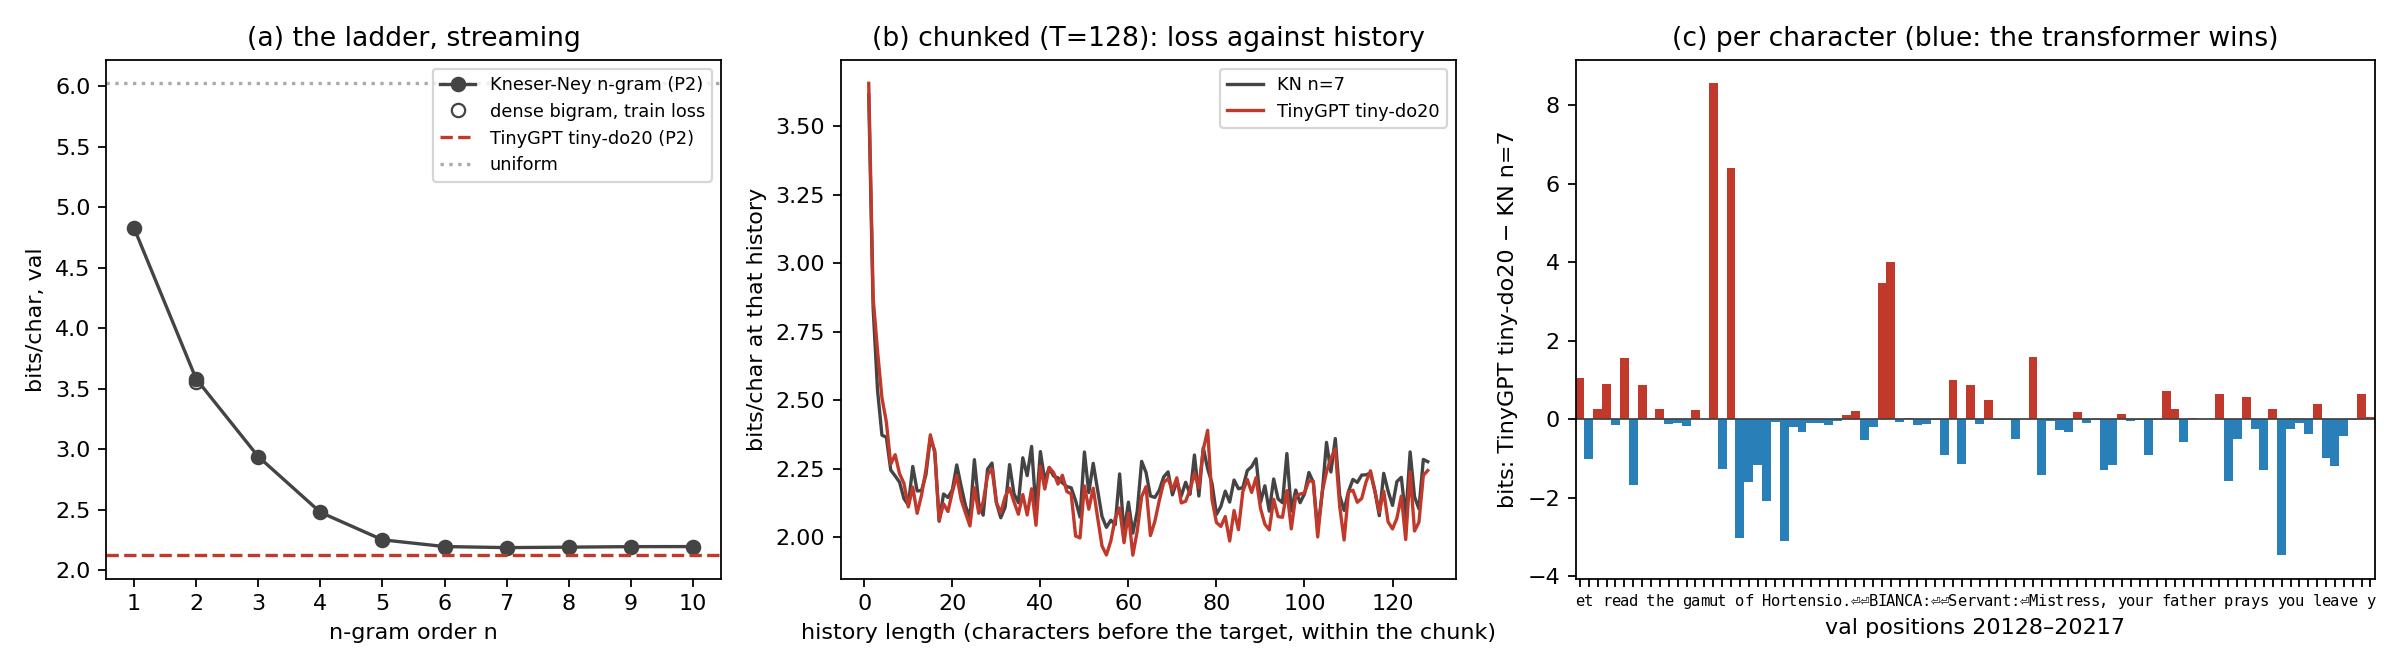
\includegraphics[width=\textwidth]{demos/tinygpt_ngram_ladder.png}
\caption{Seed 0 of the \texttt{tiny} row with residual dropout 0.2 at
10,000 steps against the ladder
(\texttt{runs/2026-10-27-tinygpt-dropout-xla/}). (a) Bits per character
against $n$-gram order; the dashed line is the transformer, the hollow
point at $n{=}2$ the dense bigram's training loss. (b) The loss at each
history length within a 128-character window, the 7-gram and the
transformer: the counts win the first ten characters, the transformer the
rest. (c) Transformer minus 7-gram along ninety held-out characters; blue
is where the transformer wins.}
\label{fig:tinygpt_ladder}
\end{figure}

\noindent \textbf{The sign is the result.} Every transformer row trained
the way the catalogue prints it is behind a six-character count on its
own corpus: nano by $0.04$ to $0.06$ bits on every seed, and the levers
that come to mind first, more steps, a bigger batch, rotary positions,
move it by hundredths and never across. \texttt{tiny}, with nearly six
times the parameters, is worse still, because on 1 MB of text it has
memorised the file by step 4,000 and spends the rest of the schedule
overfitting. The nets were not undertrained. They were unregularised.

One knob changes the sign. \texttt{.transformerEncoder (dropout := 0.2)}
puts GPT-2's residual dropout on each block's two branches and nothing
else in the recipe moves; the same \texttt{tiny} at the same 10,000 steps
is $0.06$ bits per character \emph{ahead} of the 7-gram on every seed,
every interval clear of zero. Panel~(b) of the figure says where it earns
that: behind the counts at histories under ten characters, ahead from the
eleventh on. A 7-gram sees six characters back; the transformer's margin
is all in the history the counts cannot see.

The rotary row answers one more question the catalogue raises. Positions
without a table make the checkpoint load at any $T$, but a net trained at
64 characters is not coherent at 128 or 256 ($3.1$ and $4.9$ bits per
character, seed means, against $2.28$ at its own length). The weights are
length-independent; the function is not.

\medskip\noindent What this is not: a scaling result, a tokenised model,
or a second corpus. The ladder is one file of 1 MB scored at character
level, where a 7-gram is a strong model; a byte-pair vocabulary over
gigabytes is a different comparison. And the number the transformer beats
is a count table's: the ladder says where in the window the net earned
its margin, not what it learned there.

\medskip\noindent The rest of the demo is the mechanics, and they are the
same for the regularised net as for the first one. Sampling from the
10,000-step nano checkpoint produces Shakespeare's cadence, real character
names (NORTHUMBERLAND, QUEEN MARGARET, MERCUTIO, BRUTUS) and multi-line
dialogue; the first eight characters of its \texttt{ROMEO:} sample are the
rows of Figure~\ref{fig:tinygpt_causal_mask}. Three things change relative to the
image trainers of Part~1, and they are what NLP training is:

\begin{itemize}
  \item \textbf{Input is a vocabulary index, not a pixel.} The first
    layer of every NLP spec is \texttt{.tokenPositionEmbed} (one-hot
    $\to$ learnable token embedding $+$ learnable position embedding).
    Image stacks open with \texttt{.conv2d} or \texttt{.patchEmbed}
    acting on $H \times W \times 3$ floats; the NLP stack starts with
    vocabulary IDs flowing through a lookup table. Replace patches
    with tokens and the rest of a ViT is shape-identical to a GPT.
  \item \textbf{Loss is per-token, averaged over the sequence.} Image
    classifiers compute one cross-entropy at the end of the network:
    pool to a vector, dense to logits, compare to one ground-truth
    class. Language models compute cross-entropy at every
    position --- each of the $T$ tokens predicts the next one, and the
    per-token losses are averaged. The trainer reuses the same
    cross-entropy path by setting \texttt{lossKind := some .perPixelCE}
    in its \texttt{TrainConfig}: the LM head's $[B, V, T, 1]$ logits ride
    the per-pixel path as a segmentation of $T$ positions by one column,
    which switches the loss from ``one vector
    versus one class'' to ``$T$ vectors versus $T$ classes.'' No new
    VJP machinery; the per-token softmax-CE backward is the same one
    Chapter~\ref{chap:tensor} derived, applied $T$ times in parallel.
  \item \textbf{Inference is autoregressive.} The training loop is a
    single forward pass per batch, just like image classification, but
    inference is a $T$-step loop: the network predicts token
    $t{+}1$ from tokens $[0..t]$, the sampled token is appended to the
    context, and the network runs again for $t{+}2$. The
    \texttt{tinygpt-shakespeare sample} executable implements exactly
    this loop --- $\sim$30 lines of plain Lean, no proof machinery,
    running the same spec's forward graph at batch one through XLA on
    the parameters the trainer saved. The architectural
    cost is the causal mask (Figure~\ref{fig:tinygpt_causal_mask}):
    during training, attention at position
    $t$ must not see positions $t{+}1$ onward, or the model would
    trivially predict the answer it can see. The \texttt{causalMask}
    flag on \texttt{.transformerEncoder} is that mask; the rest of the
    kit is shared with ViT.
\end{itemize}

\begin{figure}[H]
\centering
\begin{tikzpicture}[x=0.68cm, y=0.68cm, font=\small,
  live/.style={fill=blue!25, draw=blue!50!black!40, line width=0.3pt},
  dead/.style={fill=white, draw=black!25, line width=0.3pt},
  tok/.style={font=\ttfamily\small},
  hdr/.style={font=\footnotesize\itshape, text=black!70},
  arrow/.style={->, >=stealth, thick, gray}]
  % the prompt "ROMEO:", its newline, and the first sampled character of
  % runs/2026-09-09-tinygpt-nano-xla/sample_romeo.txt ("O heaven ...") -- eight char tokens, position 0..7
  \def\toks{R,O,M,E,O,:,{\textbackslash n},O}
  \def\nexts{O,M,E,O,:,{\textbackslash n},O,?}
  % grid: row t = query (top to bottom), column s = key (left to right)
  \foreach \t in {0,...,7} {
    \foreach \s in {0,...,7} {
      \pgfmathparse{\s<=\t ? 1 : 0}
      \ifnum\pgfmathresult=1
        \path[fill,live] (\s,-\t) rectangle ++(1,-1);
      \else
        \path[fill,dead] (\s,-\t) rectangle ++(1,-1);
        \node[font=\tiny, text=black!45] at (\s+0.5,-\t-0.5) {$-\infty$};
      \fi
    }
  }
  % key tokens across the top, query tokens down the left, targets down the right
  \foreach \s [count=\i from 0] in \toks {
    \node[tok, anchor=south] at (\i+0.5, 0.08) {\s};
    \node[hdr, anchor=south] at (\i+0.5, 0.55) {\i};
    \node[tok, anchor=east] at (-0.12, -\i-0.5) {\s};
    \node[hdr, anchor=east] at (-0.95, -\i-0.5) {\i};
  }
  \foreach \n [count=\i from 0] in \nexts {
    \node[tok, anchor=west] at (9.3, -\i-0.5) {\n};
    \draw[arrow] (8.15, -\i-0.5) -- (9.05, -\i-0.5);
  }
  \node[hdr, anchor=south] at (4, 1.05) {keys $s$: positions row $t$ may look at};
  \node[hdr, rotate=90, anchor=south] at (-1.6, -4) {queries $t$: position being predicted from};
  \node[hdr, anchor=south, align=center] at (9.7, 0.08) {target\\ (token $t{+}1$)};
  % the highlighted row: t = 4, the second O of ROMEO
  \draw[red!70!black, line width=1.1pt] (0,-4) rectangle (8,-5);
  \draw[red!70!black, line width=1.1pt] (9.0,-4) rectangle (10.0,-5);
  \node[font=\footnotesize, text=red!70!black, anchor=north west, align=left] at (0, -8.35)
    {row 4 sees \texttt{R O M E O} and nothing after it; its loss is the cross-entropy against \texttt{:}};
  \node[font=\footnotesize, text=black!70, anchor=north west, align=left] at (0, -9.0)
    {white cells: $-\infty$ is added to the score before the softmax, so their weight is exactly $0$};
\end{tikzpicture}
\caption{The causal mask on the sampler's first eight characters: the prompt \texttt{ROMEO:}, its newline and the first character it sampled. Rows are the
position being predicted from, columns the positions it may attend to; a score
survives (blue) only where the key is at or before the query, and $-\infty$ is
added to every other score before the softmax, so its weight is exactly zero.
Row 4 is the second O of ROMEO: it sees \texttt{ROMEO} and is scored against the
colon. At the trainer's $T{=}64$ the same triangle keeps 2080 of the 4096 scores
per head. The \texttt{causalMask} flag on \texttt{.transformerEncoder} is the
whole difference between this block and a ViT's.}
\label{fig:tinygpt_causal_mask}
\end{figure}

That's the entire delta. Same Adam optimizer, same VJP machinery, same
StableHLO-through-XLA pipeline. The catalogue entries of this section all reduce to
either ``GPT shape'' (decoder-only, causal mask, autoregressive
sampling) or ``BERT shape'' (encoder-only, bidirectional attention,
classification head); the architectural differences between them are
smaller than the chapter-to-chapter deltas in Part~1.

\subsection*{Mamba (\texttt{Bestiary/Mamba.lean})}
\emph{One} new primitive (Definition~\ref{layer:mambaBlock}). Variants: Mamba-130M / 370M / 790M /
tiny, matching Gu \& Dao's (2023,
\href{https://arxiv.org/abs/2312.00752}{arXiv:2312.00752}) param counts
within $\sim$5\%.

\begin{verbatim}
def mamba130M : NetSpec where
  name   := "Mamba-130M"
  imageH := 2048                                  -- context length (L tokens)
  imageW := 1
  layers := [
    -- dim=768, state=16, expand=2, 24 blocks
    .mambaBlock 768 16 2 24,
    .dense 768 50280 .identity                    -- LM head (GPT-NeoX vocab)
  ]
\end{verbatim}

\subsection*{BERT / RoBERTa (\texttt{Bestiary/BERT.lean})}
\emph{Zero} new primitives --- uses \texttt{.transformerEncoder}, same kit as
ViT / DETR, plus \texttt{.dense vocab$\to$dim} standing in for the
token-embedding table (faithful param count, shape semantics cheat
since a linear \texttt{NetSpec} can't express the $L \to L \times D$
lookup). Variants: BERT-base (109M, paper 110M), BERT-large (335M,
paper 340M), RoBERTa-base (124M, paper 125M), RoBERTa-large (355M,
paper-exact), tinyBERT fixture. The architectural lesson is that
RoBERTa (Liu et al.\ 2019,
\href{https://arxiv.org/abs/1907.11692}{arXiv:1907.11692}) = BERT
(Devlin et al.\ 2018,
\href{https://arxiv.org/abs/1810.04805}{arXiv:1810.04805}); all
RoBERTa gains came from training procedure
(dynamic masking, more data, bigger batches, dropped NSP) --- none
of which lives in the NetSpec.

\begin{verbatim}
def bertBase : NetSpec where
  name   := "BERT-base"
  imageH := 512                                   -- max context length
  imageW := 1
  layers := [
    -- Token-embedding lookup approximated as dense (vocab → D)
    .dense 30522 768 .identity,
    -- 12 encoder blocks, post-norm, GELU, mlpDim = 4·D
    .transformerEncoder 768 12 3072 12,
    -- [CLS] pooler (tanh applied downstream)
    .dense 768 768 .identity
  ]
\end{verbatim}

\subsection*{GPT-1 / GPT-2 (\texttt{Bestiary/GPT.lean})}
\emph{Zero} new primitives. GPT-1 (Radford et al.\ 2018,
\href{https://cdn.openai.com/research-covers/language-unsupervised/language_understanding_paper.pdf}{OpenAI TR})
and GPT-2 (Radford et al.\ 2019,
\href{https://cdn.openai.com/better-language-models/language_models_are_unsupervised_multitask_learners.pdf}{OpenAI TR})
are decoder-only counterparts of BERT. Same
\texttt{.transformerEncoder}, now read as a stack of decoder blocks
with a causal attention mask (a training-time detail, not a
parameter). No pooler; GPT-2 uses pre-norm instead of BERT's
post-norm (zero-parameter swap). Weight tying: the LM head reuses
the token-embedding matrix, so our \texttt{.dense vocab$\to$D}
stand-in already pays for both input and output sides. Variants:
GPT-1 (116M, paper 117M), GPT-2 small (123M, paper 124M), medium
(353M), large (772M, paper 774M), XL (1.56B, paper 1.5B), tinyGPT
fixture. Reference implementation: Karpathy's \texttt{nanoGPT}
($\sim$300 lines of PyTorch) targets GPT-2 small and is the
canonical mental model.

\begin{verbatim}
def gpt2Small : NetSpec where
  name   := "GPT-2 small"                         -- the nanoGPT target
  imageH := 1024                                  -- context length
  imageW := 1
  layers := [
    -- Tied token embedding (also serves as LM head projection)
    .dense 50257 768 .identity,
    -- 12 decoder blocks, pre-norm (mask is attention-time, not a param)
    .transformerEncoder 768 12 3072 12 (causalMask := true)
  ]
\end{verbatim}

\subsection*{QANet (\texttt{Bestiary/QANet.lean})}
\emph{One} new primitive (\texttt{.separableConv}). The 2018 reading-comprehension
architecture that killed the BiLSTM for SQuAD-style tasks (Yu et al.\ 2018,
\href{https://arxiv.org/abs/1804.09541}{arXiv:1804.09541}). Core contribution: an encoder block combining 4 depthwise-
separable convs (local context) with a self-attention + FFN
transformer block (global context) --- the ``conv + attention
hybrid'' shape MobileViT and ConvNeXt rediscovered in 2022.
Expressed with primitives we already have: 4
\texttt{.separableConv 128 128 1} calls + 1
\texttt{.transformerEncoder 128 8 512 1} per block. Per-block count:
$\sim$270K for the embedding-encoder block; the model-encoder blocks carry
two separable convs rather than four, and the paper's seven-block stack lands
at $\sim$1.6M, repeated 3 times in the full architecture. The BiDAF-
style context-query attention and character/word embedding tables
are omitted from the spec; described in prose. QANet's headline
number was \textbf{3--4$\times$ training speedup} over BiLSTM-based
competitors, a clean example of hardware (parallelization of convs
vs. sequential RNN roll-outs) forcing an architectural choice.
BERT landing 7 months later ended the SQuAD-as-benchmark era, but
QANet's hybrid shape lived on --- showed up repeatedly in vision
4 years later.

\begin{verbatim}
def qanetEncoderBlock : NetSpec where
  name   := "QANet encoder block (4× sep-conv + self-attn + FFN)"
  imageH := 400                                   -- representative context length
  imageW := 1
  layers := [
    -- 4 depthwise-separable convs (local context, kernel 7 in paper)
    .separableConv 128 128 1,
    .separableConv 128 128 1,
    .separableConv 128 128 1,
    .separableConv 128 128 1,
    -- Self-attention + FFN + 2 LayerNorms (global context)
    .transformerEncoder 128 8 512 1
  ]
\end{verbatim}

\subsection*{Nyströmformer (\texttt{Bestiary/Nystromformer.lean})}
\emph{Zero} new primitives. An efficient-attention transformer
(Xiong et al.\ 2021,
\href{https://arxiv.org/abs/2102.03902}{arXiv:2102.03902}) that
replaces the $O(n^2)$ softmax attention
with an $O(n)$ Nyström-approximation computed via $m$ landmark
tokens, $m \ll n$. Crucially, this is a compute change, not
a parameter change: the $W_Q / W_K / W_V / W_O$ projections and the
FFN are identical to a standard transformer. Our
\texttt{.transformerEncoder} spec is therefore identical to
BERT's at each scale --- base lands at 108M (vs BERT-base 109M),
large at 333M (vs BERT-large 335M). The entry's pedagogical value is
prose-level: most of the 2020--2022 efficient-attention literature
(Linformer, Performer, Longformer, BigBird, Reformer,
FlashAttention) is parameter-identical to vanilla attention, and the
bestiary can't differentiate them at the layer level. Nyströmformer
is worth highlighting because the specific trick --- a 1930 result
from numerical linear algebra, routed through kernel-method
literature in the early 2000s, finally surfacing in transformers ---
is a genuinely long arc for one math idea.

\begin{verbatim}
def nystromformerBase : NetSpec where
  name   := "Nyströmformer base (BERT-base-shaped, O(n) attention)"
  imageH := 4096                                  -- long context
  imageW := 1
  layers := [
    -- Architecturally identical to BERT-base; Nyström approximation
    -- lives inside the attention kernel, not the NetSpec.
    .dense 30522 768 .identity,
    .transformerEncoder 768 12 3072 12
  ]
\end{verbatim}

\section{Image generation}

Networks whose output is a novel image. Two families covered here:
variational autoencoders and GANs. Backbones overlap heavily with
segmentation (UNet again). Diffusion models, also generative, are
\S~\ref{sec:bestiary_diffusion}.

\subsection*{VAE (\texttt{Bestiary/VAE.lean})}
\emph{One} new primitive (Definition~\ref{layer:unetUp}). The classical variational autoencoder
(Kingma \& Welling 2013, \href{https://arxiv.org/abs/1312.6114}{arXiv:1312.6114}): encoder outputs
$(\mu, \log \sigma^2)$ (represented as a single tensor with doubled
final width), the reparameterization trick
$z = \mu + \sigma \odot \epsilon$ samples $z$ in training code, the
decoder reconstructs. KL divergence between the learned latent
distribution and a standard normal is the regularizer. Variants:
MNIST MLP VAE (20-dim latent, textbook example), CIFAR conv VAE
($4 \times 4 \times 4$ spatial latent, SD-style), tiny fixture. All
shown as encoder + decoder pairs. Training-code details (the actual
sampling step, the KL loss) live outside the NetSpec. The same
architectural template scales up to Stable Diffusion's VAE (see
\texttt{StableDiffusion.lean}); 2013's 20-dim MNIST latent and
2022's $64 \times 64 \times 4$ SD latent are the same idea at
different scales. VQ-VAE (discrete-codebook variant) and $\beta$-VAE
(scaled KL) are mentioned in the prose notes.

\begin{verbatim}
def mnistVAEEncoder : NetSpec where
  name   := "MNIST VAE encoder (MLP, 20-dim latent)"
  imageH := 28
  imageW := 28
  layers := [
    .flatten,
    .dense 784 400 .relu,
    -- Output is 2×20 = 40: first 20 are μ, last 20 are log σ².
    .dense 400 40 .identity
  ]
\end{verbatim}

\subsection*{DCGAN (\texttt{Bestiary/DCGAN.lean})}
\emph{Zero} new primitives. Deep Convolutional GAN (Radford et
al.\ 2015, \href{https://arxiv.org/abs/1511.06434}{arXiv:1511.06434}) --- the paper that made GAN training reliably work. Five
design guidelines (strided convs instead of pooling, BN everywhere
except $G$'s output / $D$'s input, no hidden FC layers, ReLU in $G$,
LeakyReLU in $D$), plus an Adam recipe, that became the
default for every GAN paper since. Three NetSpecs: noise projector
(dense $100 \to 4 \times 4 \times 1024$, 1.65M), generator convs
(11M, paper $\sim$12M), discriminator (11M, paper-exact). Transposed
convs in $G$ are approximated by standard convs of matching kernel
and channels (same params, spatial doubling is forward-pass-only);
same hack appears in VAE and Stable Diffusion entries. GAN training
dynamics (mode collapse, equilibrium stability) are all
training-procedure concerns living outside the NetSpec.

\begin{verbatim}
def dcganGenerator : NetSpec where
  name   := "DCGAN generator (64×64 RGB)"
  imageH := 4                                     -- starting spatial (post-projection)
  imageW := 4
  layers := [
    -- Each .convBn stands in for a 4×4 transposed conv doubling spatial;
    -- same params (ic × oc × k²), upsampling is a forward-pass detail.
    .convBn 1024 512 4 1 .same,                  --  4×4 →  8×8
    .convBn 512  256 4 1 .same,                  --  8×8 → 16×16
    .convBn 256  128 4 1 .same,                  -- 16×16 → 32×32
    .convBn 128   64 4 1 .same,                  -- 32×32 → 64×64
    .conv2d   64   3 4 .same .identity           -- RGB output (tanh in real)
  ]
\end{verbatim}

\subsection*{Pix2Pix (\texttt{Bestiary/Pix2Pix.lean})}
\emph{Two} new primitives (Definition~\ref{layer:unetDown}, Definition~\ref{layer:unetUp}). The paired-data ancestor of CycleGAN,
from the same lab 9 months earlier (Isola et al.\ 2017,
\href{https://arxiv.org/abs/1611.07004}{arXiv:1611.07004}). UNet
generator (8 levels, $\sim$62M vs paper $\sim$54M --- our
\texttt{.unetDown} / \texttt{.unetUp} use 2 convs per level where
Pix2Pix uses 1 strided conv, so we overcount) + PatchGAN
discriminator (identical to CycleGAN's, 2.8M). Trained with GAN
loss + L1 reconstruction --- the L1 term is a direct supervision
signal that exists only because pairs exist. When you don't have
pairs you fall back to CycleGAN's cycle-consistency trick. Hardware
context: 2016--2017, 54M UNet on $256 \times 256$ images meant
batch size 1 on a GTX 1080 Ti, which is how InstanceNorm became the
default normalizer in this lineage --- it was what fit.

\begin{verbatim}
def pix2pixGenerator : NetSpec where
  name   := "Pix2Pix generator (8-level UNet, 256×256 RGB)"
  imageH := 256
  imageW := 256
  layers := [
    -- Encoder: 8 × unetDown, channels 64 → 128 → 256 → 512 → 512 ×4
    .unetDown 3    64, .unetDown 64  128,
    .unetDown 128 256, .unetDown 256 512,
    .unetDown 512 512, .unetDown 512 512,
    .unetDown 512 512, .unetDown 512 512,         -- bottleneck at 1×1×512
    -- Decoder: 8 × unetUp mirroring the encoder
    .unetUp 512 512, .unetUp 512 512,
    .unetUp 512 512, .unetUp 512 512,
    .unetUp 512 512, .unetUp 512 256,
    .unetUp 256 128, .unetUp 128  64,
    .conv2d 64 3 1 .same .identity                -- 1×1 to RGB (tanh in real)
  ]
\end{verbatim}

\subsection*{CycleGAN (\texttt{Bestiary/CycleGAN.lean})}
\emph{Zero} new primitives. Unpaired image translation (Zhu et
al.\ 2017, \href{https://arxiv.org/abs/1703.10593}{arXiv:1703.10593}): two generators $G : X \to Y$ and $F : Y \to X$ plus two
PatchGAN discriminators, trained with adversarial loss + cycle
consistency loss $\|F(G(x)) - x\|_1$. The cycle constraint is what
makes unpaired training work --- without it, $G$ could mode-collapse
every $x$ to one target. Generator is a Johnson-style ResNet (Johnson et al.\ 2016,
\href{https://arxiv.org/abs/1603.08155}{arXiv:1603.08155}):
convs down + 9 \texttt{.residualBlock}s at 256 channels + convs up
(11.4M, paper $\sim$11M). Discriminator is a PatchGAN: 5 strided
convs with a $70 \times 70$ receptive field, outputs an $N \times N$
grid of patch real/fake logits (2.8M, paper $\sim$2.8M). Four-network
pattern shown as two specs ($G$ and $D$); the other $F$ and
$D_X$ are architecturally identical copies. The ``one clever loss''
does the work --- the architecture is quite ordinary.

\begin{verbatim}
def cycleganGenerator : NetSpec where
  name   := "CycleGAN generator (9-block ResNet, 256×256 RGB)"
  imageH := 256
  imageW := 256
  layers := [
    .convBn 3 64 7 1 .same,                       -- 7×7 stem
    .convBn 64  128 3 2 .same,                    -- 256 → 128
    .convBn 128 256 3 2 .same,                    -- 128 →  64
    .residualBlock 256 256 9 1,                   -- 9 res blocks (bottleneck)
    .convBn 256 128 3 1 .same,                    -- upsample stand-in
    .convBn 128  64 3 1 .same,
    .conv2d 64 3 7 .same .identity                -- 7×7 to RGB
  ]
\end{verbatim}

\section{Diffusion --- demo: DDPM on MNIST}
\label{sec:bestiary_diffusion}

A network trained only to predict the noise added to a clean image draws new
images by iterating the reverse (noise in, image out). The architecture is a UNet
--- often with cross-attention bolted in for text conditioning; what is new is the
noise schedule and the sampling loop, not a layer. Two questions a grid of samples
cannot answer: \emph{how good are the samples, measured, and which sampler should
run on the trained weights?}

\paragraph{DDPM on MNIST.} The \texttt{demos/MainMnistDdpmTrain.lean} trainer
is a timestep-conditioned UNet trained to predict the Gaussian noise added to an
image; \texttt{mnist-ddpm-sample} runs the reverse loop and writes a grid. The
backbone is literally the segmentation UNet of
\S~\ref{sec:bestiary_segmentation}. Three things
change relative to the classifiers, segmentation nets and detectors so far:

\begin{itemize}
  \item \textbf{The target is the noise, and it is self-supervised.} Every model
    so far compares against something a human provided --- a class, a mask, a
    set of boxes. Diffusion manufactures its own: sample a timestep $t$, sample
    noise $\varepsilon$, add it per the schedule, predict $\varepsilon$, under
    the same squared-error backward from Part~1 (the demo compiles its own
    train step, with \texttt{useDdpm := true}).
  \item \textbf{The backbone is the segmentation UNet, conditioned on $t$.} One
    network must denoise at every level, so $t$ is fed in: this demo
    concatenates it as an extra channel (hence \texttt{.unetDown 2 16} --- one
    image channel plus one time channel), and the catalogue's DDPM entry embeds it
    through a sinusoidal MLP, the positional-encoding primitive NeRF introduced.
    Diffusion adds only the conditioning.
  \item \textbf{Inference is an iterative loop, not one forward pass.} What that
    loop costs is Table~\ref{tab:ddpm_samplers}.
\end{itemize}

\paragraph{Scoring it needs an instrument, not an eye.} Unconditional image
generation is the only demo in this book whose success criterion is ``does that
look like a digit to you.'' It does not have to be: Chapter~\ref{chap:cnn}'s
verified CNN maps an image to ten numbers, and in that space the usual
statistics work. What matters more than any row is that the scale is
bracketed at both ends, since a metric that only ever reports ``bad'' is
indistinguishable from a broken one. Table~\ref{tab:ddpm_scores} is the bracket.

\begin{table}[H]
\centering
\caption{Generated MNIST scored by the verified CNN, bracketed by real data and by unstructured pixels; the energy floor is real against real, $0.0016$.}
\label{tab:ddpm_scores}
\begin{tabular}{@{}l c c r c@{}}
\hline
& coverage & confidence & energy ($\times$ floor) & pixel mean \\
\hline
real MNIST, scored as if generated & 10/10 & $99.40\%$ & $0.0020$ \;($1.2\times$)  & $0.122$ \\
the model, ancestral sampling      & 10/10 & $92.98\%$ & $0.0067$ \;($4\times$)  & $0.118$ \\
the model, deterministic DDIM      & 10/10 & $90.94\%$ & $0.0237$ \;($15\times$) & $0.138$ \\
unstructured pixels                &  4/10 & $58.47\%$ & $0.3674$ \;($231\times$)& $0.132$ \\
\hline
\end{tabular}
\end{table}

\noindent The instrument scores $98.66\%$ on the real split, which is the check
that its weights loaded. A checkpoint that writes pixels outside $[0,1]$
fails the bracket before anyone looks at a grid.
$\triangleright$ And read the confidence column against the others: noise still
posts $58\%$, so the usable range is $58$--$99$ rather than $0$--$100$, and on
its own it is the metric most likely to mislead.

\paragraph{The continuous-time view, and which solver to use.} The trainer and
the two samplers of Table~\ref{tab:ddpm_scores} are discrete: a schedule tabulated
at $t = 0 \dots T{-}1$ and a fixed reverse recipe. Score-SDE (Song et al.\ 2021,
\href{https://arxiv.org/abs/2011.13456}{arXiv:2011.13456}) reads the same object as a stochastic
differential equation in continuous time, $\mathrm{d}x = f(x,t)\,\mathrm{d}t +
g(t)\,\mathrm{d}w$, whose reverse is driven by the score
$\nabla_x \log p_t(x)$. \textbf{That view costs no retraining here}, which is
the point worth taking away: under the variance-preserving SDE the score is
$-\hat\varepsilon(x,t)/\sigma_t$, so the $\varepsilon$-predicting network
\texttt{MainMnistDdpmTrain.lean} already produces is a score model up to a scale factor.
Sampling is then whatever you choose to integrate, on frozen weights: the
reverse SDE, its deterministic twin the probability-flow ODE, or the family
between them that DDIM's $\eta$ (Song, Meng \& Ermon 2020,
\href{https://arxiv.org/abs/2010.02502}{arXiv:2010.02502}) interpolates.

So it can be measured. Energy distance against real MNIST, budget in network
evaluations:

\begin{table}[H]
\centering
\caption{Energy distance to real MNIST by sampler and number of network evaluations.}
\label{tab:ddpm_samplers}
\begin{tabular}{@{}l c c c c@{}}
\hline
sampler & NFE $10$ & NFE $20$ & NFE $50$ & NFE $200$ \\
\hline
DDIM, $\eta = 0$ (deterministic) & $0.0874$ & $0.0437$ & $0.0237$ & $0.0188$ \\
DDIM, $\eta = 1$ (ancestral)     & $\mathbf{0.0455}$ & $\mathbf{0.0132}$ & $\mathbf{0.0067}$ & $\mathbf{0.0099}$ \\
reverse SDE (Euler--Maruyama)    & $1.1837$ & $0.9870$ & $0.3382$ & $0.0211$ \\
probability-flow ODE (Euler)     & $0.3542$ & $0.2053$ & $0.0910$ & $0.0288$ \\
\hline
\end{tabular}
\end{table}

\noindent \textbf{Noise in the reverse process helps, and the effect is
monotone in $\eta$ at every budget} --- the two intermediate arms, $\eta = 0.25$
and $\eta = 0.5$, sit in order between the first two rows. Ancestral sampling at
$50$ evaluations beats the deterministic sampler at $200$ by nearly $3\times$,
on a quarter of the compute. Figure~\ref{fig:ddpm_mnist} is the process itself,
forward and reverse.

\begin{figure}[H]
\centering
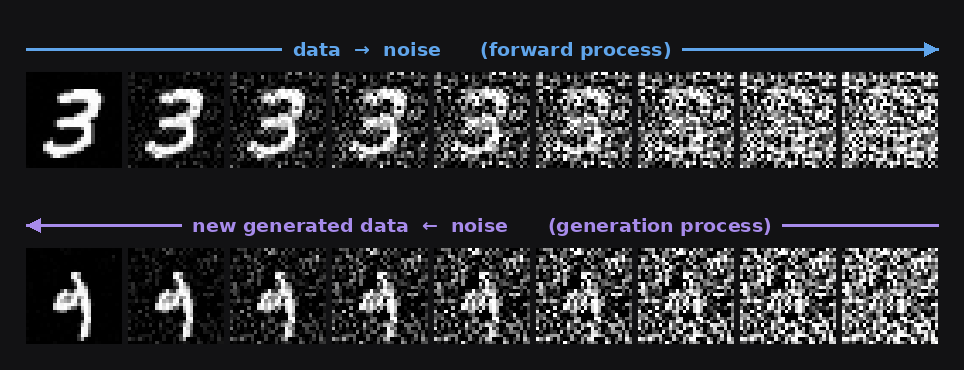
\includegraphics[width=\textwidth]{demos/ddpm_mnist_trajectory.png}
\caption{DDPM on MNIST, both directions, nine columns aligned by noise level.
Top: the forward process takes a training digit to Gaussian noise. Bottom: the
trained reverse process under deterministic DDIM ($\eta = 0$), started from
fresh noise, at the same nine noise levels.}
\label{fig:ddpm_mnist}
\end{figure}

\medskip\noindent Which makes the third row the instructive one. The
reverse SDE and ancestral sampling are the same idea --- integrate the
stochastic reverse process --- and they land at opposite ends of this table,
because one of them discretises it well and the other does not. The reverse
process is stiff, $\beta(t)$ diverging as $t \to 1$, and the Euler--Maruyama arm
diverges below $200$ evaluations (pixel mean $2.90$ against the data's $0.13$,
two classes of ten covered) while posting the highest confidence in this
section --- the warning under Table~\ref{tab:ddpm_scores} arriving from a second direction.
The probability-flow row lags for the same reason, more mildly. So the choice
that matters here is not stochastic versus deterministic; it is how the linear
part gets integrated, and DDIM does it exactly at either $\eta$.

The shape carries all the way up: the DDPM catalogue entry that closes this section
is the same UNet at CIFAR scale, and Stable Diffusion is the same UNet on VAE latents with text
cross-attention spliced in. Encoder-decoder-with-skips plus a sampling loop is
the whole generative pipeline.

\subsection*{DDPM (\texttt{Bestiary/Diffusion.lean})}
\emph{Three} new primitives (Definition~\ref{layer:unetDown}, Definition~\ref{layer:unetUp}, Definition~\ref{layer:positionalEncoding}). The denoiser in Ho et al.'s DDPM (2020,
\href{https://arxiv.org/abs/2006.11239}{arXiv:2006.11239}) is a UNet
--- literally the same Definition~\ref{layer:unetDown} and
Definition~\ref{layer:unetUp} Ronneberger shipped in 2015. Everything ``diffusion'' lives in the training loop:
a forward noise schedule adds Gaussian noise over $T$ steps, a reverse
process learns to predict the added noise, sampling iterates the
reverse from pure noise back to a clean image. None of that is a
layer. The timestep conditioning MLP (sinusoidal $\to$ dense $\to$
dense) is shown as a standalone \texttt{NetSpec} that reuses
\texttt{positionalEncoding} from NeRF. Variants: CIFAR config ($32\times32$
backbone), $256\times256$ high-res config, tiny fixture, timestep embed.
Our simplified backbone undercounts vs paper (paper DDPM adds
residual blocks, GroupNorm, attention-at-low-res, and per-block
time-embedding projection on top of the UNet); the spec's value is
showing the architectural shape, not an exact param match. The
lesson is the same one CLIP and NeRF taught: the novelty lives in
the training procedure, not in layer design.

\begin{verbatim}
def ddpmCifar : NetSpec where
  name   := "DDPM (CIFAR-10, backbone approx)"
  imageH := 32
  imageW := 32
  layers := [
    -- Encoder: 32 → 16 → 8 → 4
    .unetDown 3   128,                            -- 32 → 16
    .unetDown 128 256,                            -- 16 →  8
    .unetDown 256 256,                            --  8 →  4
    .convBn 256 256 3 1 .same,                    -- bottleneck
    .convBn 256 256 3 1 .same,
    -- Decoder: 4 → 8 → 16 → 32
    .unetUp 256 256, .unetUp 256 256, .unetUp 256 128,
    .conv2d 128 3 1 .same .identity               -- predict added noise (3-ch)
  ]
\end{verbatim}

\subsection*{Stable Diffusion (\texttt{Bestiary/StableDiffusion.lean})}
\emph{Three} new primitives (Definition~\ref{layer:unetDown}, Definition~\ref{layer:unetUp}, Definition~\ref{layer:transformerDecoder}). The paper that made generative image
models consumer-reachable (Rombach et al.\ 2022,
\href{https://arxiv.org/abs/2112.10752}{arXiv:2112.10752}). Two architectural
moves over DDPM, each individually small: (a) \emph{latent diffusion}
--- run the diffusion process on 64$\times$64$\times$4 VAE latents
instead of 512$\times$512 pixels, cutting spatial work $\sim$64$\times$;
(b) \emph{text conditioning via cross-attention} --- at each interior
UNet resolution, insert a spatial transformer block that cross-attends
from image tokens to CLIP text embeddings. Shown as six separate
NetSpecs: VAE encoder, VAE decoder, CLIP text encoder (123M, matches
CLIP ViT-L/14 exactly), UNet backbone (190M backbone approx; real
SD 1.5 UNet is 865M, missing $\sim$675M is the interleaved
cross-attention), an explicit spatial-transformer-block spec (uses
\texttt{.transformerDecoder} with \texttt{nQueries = 0} --- same
primitive Whisper's decoder uses, same mechanism as DETR's decoder
applied at image-feature resolution), and a tiny end-to-end fixture.
Two components are pretrained and frozen during SD's main training,
the VAE and the CLIP text encoder; only the UNet trains. SDXL scales the UNet to 2.6B; SD 3
switches the UNet for a DiT transformer. The latent-diffusion plus
text-conditioning template is the same.

\begin{verbatim}
def sdUNet15 : NetSpec where
  name   := "SD 1.5 UNet denoiser (backbone approx)"
  imageH := 64                                    -- latent resolution, not pixel
  imageW := 64
  layers := [
    .conv2d 4 320 3 .same .identity,              -- stem (latent → channels)
    -- Encoder: 64 → 32 → 16 → 8
    .unetDown 320  640,
    .unetDown 640  1280,
    .unetDown 1280 1280,
    -- Bottleneck at 8×8 (real SD inserts a spatial transformer here)
    .convBn 1280 1280 3 1 .same,
    .convBn 1280 1280 3 1 .same,
    -- Decoder: 8 → 16 → 32 → 64
    .unetUp 1280 1280,
    .unetUp 1280 1280,
    .unetUp 1280 640,
    .conv2d 640 4 3 .same .identity               -- predict noise (4-ch latent)
  ]
\end{verbatim}

\section{Physics --- demo: Boltzmann generator on M\"uller--Brown}
\label{sec:bestiary_boltzmann}

Networks whose target is a physical law rather than a labelled set: a
Boltzmann density in the demo, a PDE residual, a solution operator and the
atmosphere six hours ahead in the catalogue entries. The architectural side is
small --- an MLP, or a ViT with a Fourier mixer where its attention would be
--- and the novelty lives in what the model is asked to produce and in what
is done with it afterwards.

\paragraph{A Boltzmann generator.} The target is not a dataset. It is a
density, $\exp(-U/kT)$ on the three-well surface M\"uller and Brown proposed
in 1979 as the test case for reaction paths, and the training set is whatever
overdamped Langevin manages to produce at $kT = 20$ in a fixed budget: eight
chains of $10^5$ steps, the Euler--Maruyama integrator the diffusion demo's
table (\S~\ref{sec:bestiary_diffusion}) retired as a sampler, doing its actual
job. The network is an MLP, the one the 2-D diffusion trainer
(\texttt{demos/MainDiffusion2d.lean}, the MNIST demo's loss on point clouds
in the plane) fits: $18{,}178$ parameters, two hidden layers of 128, the image
path's sincos time encoding at $H = W = 1$. The loss is that trainer's rank-2
squared-error block,
and the \texttt{flow} flag changes one thing in the trainer, the interpolant:
$x_t = (1-t)\,x_0 + t\,\varepsilon$ with target $\varepsilon - x_0$ (Lipman et
al.\ 2022, \href{https://arxiv.org/abs/2210.02747}{arXiv:2210.02747}) in place
of the cosine-schedule $x_t$ with target $\varepsilon$. The sampler is Euler on
$\mathrm{d}x/\mathrm{d}t = v_\theta(x, t)$ from $t = 1$ to $0$. Three things
change relative to the MNIST demo:

\begin{itemize}
  \item \textbf{The ground truth is a formula.} $U$ has a closed form, so the
    well populations, the mean energy, the free-energy difference between
    wells and the exact likelihood are all numbers by quadrature on a
    $360 \times 360$ grid. Every column of Tables~\ref{tab:boltzmann_kt20}
    and \ref{tab:boltzmann_reweight} is exact for the quadrature row.
  \item \textbf{A sample set is a free-energy estimate.} $\Delta F_{AB} =
    -kT \ln (p_A / p_B)$ is read off the populations, and populations are
    assigned by gradient descent to a minimum rather than by nearest minimum,
    because the wells are elongated and Voronoi cells put part of A's basin
    in C.
  \item \textbf{Temperature is a knob the trained model can be moved along
    without retraining.} Every sample carries its own log-density: the
    Jacobian of each Euler step is two central differences in 2-D, and
    $\log|\det(I + h\,\partial v/\partial x)|$ integrated beside the state is
    the continuity equation for the map actually run. With it, the
    importance weight $\exp(-U/kT') / p_\theta(x)$ is a number, and that is
    the Boltzmann generator of No\'e et al.\ 2019
    (\href{https://doi.org/10.1126/science.aaw1147}{Science 365}), on an
    18k-parameter MLP.
\end{itemize}

Figure~\ref{fig:boltzmann_mb} is the surface, the trained flow, and the
reweighting that the chain cannot do.

\begin{figure}[H]
\centering
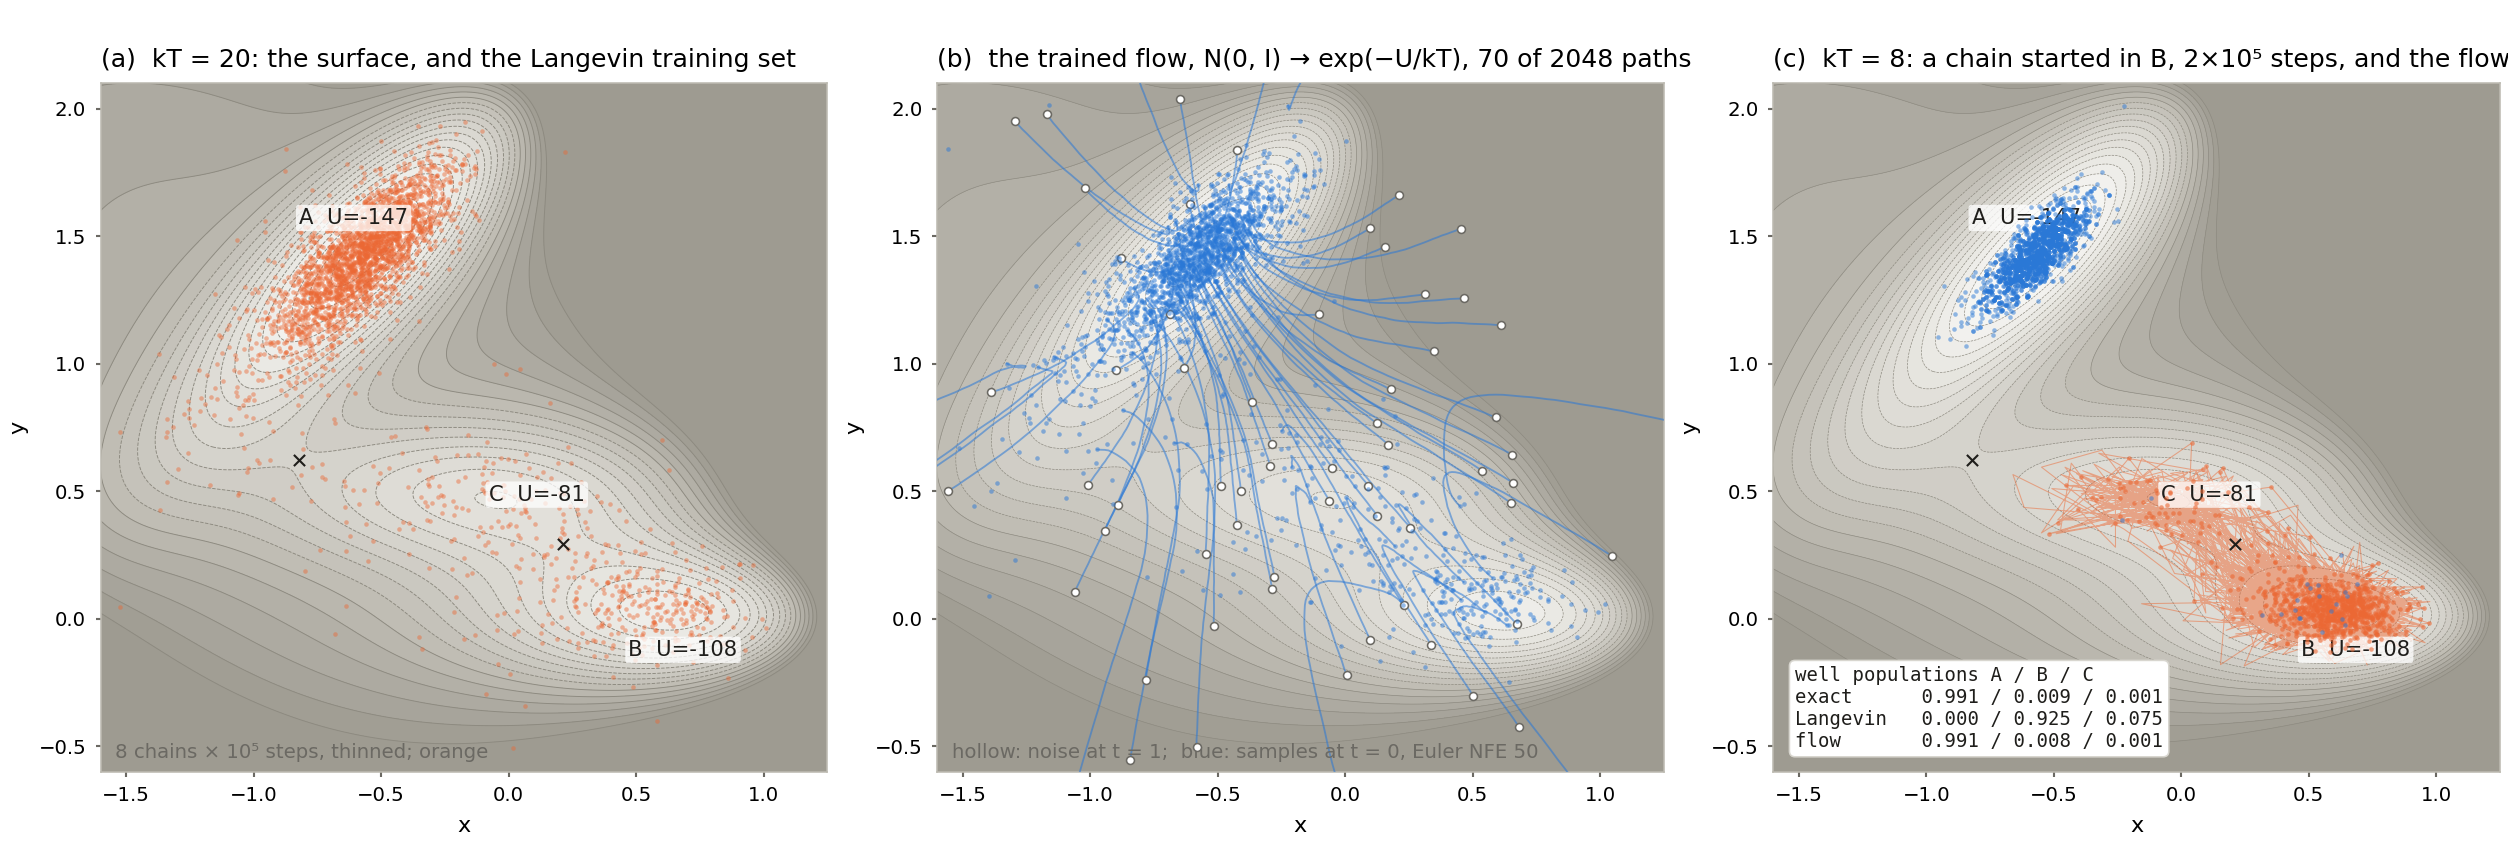
\includegraphics[width=\textwidth]{demos/boltzmann_mb.png}
\caption{A Boltzmann generator on the M\"uller--Brown surface. (a) The
potential, three minima and two saddles, with the training set: eight
overdamped Langevin chains at $kT = 20$. (b) The trained flow from $N(0, I)$
into the wells in fifty Euler steps, seventy of the $2{,}048$ paths, hollow at
the noise end, and every sample at $t = 0$. (c) At $kT = 8$ a chain started in
well B and run for $2 \times 10^5$ steps never crosses the barrier; the model's
samples, drawn once at $kT = 20$ and reweighted, report the quadrature
populations to within $0.001$.}
\label{fig:boltzmann_mb}
\end{figure}

\paragraph{Scored by quadrature, not by eye.} $kT = 20$, $2{,}048$ samples per
row, the energy distance against an independent exact draw as a multiple of
the exact-against-exact floor. The DDPM row is the same network, loss and
budget with the cosine-schedule interpolant and DDIM in place of Euler:

\begin{table}[H]
\centering
\caption{The Boltzmann generator at $kT = 20$ against quadrature: well populations, mean energy, free-energy difference and energy distance.}
\label{tab:boltzmann_kt20}
\small
\begin{tabular}{@{}l c r r r@{}}
\hline
source & $p_A \,/\, p_B \,/\, p_C$ & $\langle U \rangle$ & $\Delta F_{AB}$ & energy ($\times$ floor) \\
\hline
quadrature (exact)                        & $0.806 \,/\, 0.129 \,/\, 0.065$ & $-113.6$ & $-36.6$ & $1\times$ \;($0.0015$) \\
Langevin training set, $8 \times 10^5$ steps & $0.844 \,/\, 0.101 \,/\, 0.054$ & $-112.6$ & $-42.4$ & $4.1\times$ \\
flow, Euler, NFE 50                       & $0.834 \,/\, 0.103 \,/\, 0.063$ & $-112.4$ & $-41.9$ & $\mathbf{3.2\times}$ \\
\quad reweighted by $p_{20} / p_\theta$   & $0.805 \,/\, 0.129 \,/\, 0.066$ & $-112.8$ & $-36.7$ & --- \\
flow, Euler, NFE 10                       & $0.840 \,/\, 0.086 \,/\, 0.073$ & $-117.7$ & $-45.5$ & $8.6\times$ \\
flow, Euler, NFE 2                        & $0.891 \,/\, 0.006 \,/\, 0.103$ &  $-97.4$ & $-98.9$ & $91\times$ \\
DDPM, DDIM, NFE 50                        & $0.895 \,/\, 0.059 \,/\, 0.046$ & $-114.7$ & $-54.4$ & $18\times$ \\
$N(0, I)$ prior, no flow                  & $0.419 \,/\, 0.195 \,/\, 0.385$ &   $57.2$ & $-15.3$ & $306\times$ \\
\hline
\end{tabular}
\end{table}

\noindent The model is faithful to its training set, not to the physics: it
over-weights A because the Langevin chains do. Reweighting its own samples by
$p_{20} / p_\theta$ recovers the quadrature populations to within $0.001$ and
$\Delta F$ to $0.1$ on this checkpoint, to within $0.008$ and $1.5$ over four
training seeds (Table~\ref{tab:boltzmann_seeds}), and $\langle U \rangle$ to
about a unit. At NFE 2 well B empties while the populations still look
plausible, which is why $\langle U \rangle$ and $\Delta F$ are columns.

\paragraph{Four seeds of the flow.} Table~\ref{tab:boltzmann_kt20} is one
checkpoint. Three more trainings of the flow arm under seeds 1--3 --- the seed
moves the He initialisation and the sampling noise; 33 seconds each on one
card --- sampled at NFE 50 and scored the same way are
Table~\ref{tab:boltzmann_seeds} (\texttt{runs/2026-10-27-boltzmann-seeds/};
seed 0 is \texttt{runs/2026-09-11-boltzmann-generator/}).

\begin{table}[H]
\centering
\caption{The flow arm at $kT = 20$ over four training seeds, $2{,}048$ samples at NFE 50: the raw samples, and the same samples reweighted by $p_{20} / p_\theta$, against the quadrature row of Table~\ref{tab:boltzmann_kt20} ($0.806 \,/\, 0.129 \,/\, 0.065$, $-113.6$, $-36.6$).}
\label{tab:boltzmann_seeds}
\small
\begin{tabular}{@{}c c r r r c r r@{}}
\hline
seed & raw $p_A \,/\, p_B \,/\, p_C$ & $\langle U \rangle$ & $\Delta F_{AB}$ & energy & reweighted $p_A \,/\, p_B \,/\, p_C$ & $\Delta F_{AB}$ & ESS \\
\hline
0 & $0.834 \,/\, 0.103 \,/\, 0.063$ & $-112.4$ & $-41.9$ & $3.2\times$ & $0.805 \,/\, 0.129 \,/\, 0.066$ & $-36.7$ & $1864$ \\
1 & $0.843 \,/\, 0.095 \,/\, 0.062$ & $-114.9$ & $-43.6$ & $5.3\times$ & $0.810 \,/\, 0.125 \,/\, 0.065$ & $-37.3$ & $1895$ \\
2 & $0.832 \,/\, 0.099 \,/\, 0.070$ & $-113.3$ & $-42.6$ & $3.6\times$ & $0.801 \,/\, 0.129 \,/\, 0.071$ & $-36.6$ & $1866$ \\
3 & $0.838 \,/\, 0.090 \,/\, 0.071$ & $-110.6$ & $-44.6$ & $6.3\times$ & $0.813 \,/\, 0.121 \,/\, 0.066$ & $-38.1$ & $1740$ \\
\hline
\end{tabular}
\end{table}

\noindent The energy distance is $3.2$--$6.3\times$ the floor on four seeds.
The raw cloud puts $0.832$--$0.843$ on well A on every seed, between the
training set's $0.844$ and the quadrature's $0.806$: a raw basin error of
$0.03$--$0.04$ is the training set's bias reproduced, not a property of the
seed, and the $0.029$ of seed 0 is the low end of it. The number that is a
property of the recipe is the reweighted row: every basin within $0.008$ of
quadrature on all four seeds, $\Delta F_{AB}$ within $1.5$, an effective
sample size of $1{,}740$--$1{,}895$ of $2{,}048$. The sampler-quality claim
rests on that row. Tables~\ref{tab:boltzmann_reweight} and
\ref{tab:boltzmann_reflow} read the seed-0 checkpoint only.

\paragraph{MCMC stalls below the barrier; the generator does not.} The
$kT = 20$ samples reweighted to $kT' = 12$ and $8$, naively and with the
model's density in the weight, against a Langevin chain of $2 \times 10^5$
steps started in well B:

\begin{table}[H]
\centering
\caption{Reweighting to lower temperatures, against a Langevin chain started in well B.}
\label{tab:boltzmann_reweight}
\small
\begin{tabular}{@{}r l c r r r@{}}
\hline
$kT'$ & source & $p_A \,/\, p_B \,/\, p_C$ & $\Delta F_{AB}$ & ESS \\
\hline
12 & quadrature (exact)                        & $0.949 \,/\, 0.042 \,/\, 0.009$ & $-37.4$ & --- \\
   & Langevin from B, $2 \times 10^5$ steps    & $0.869 \,/\, 0.103 \,/\, 0.029$ & $-25.6$ & --- \\
   & flow at $kT = 20$, reweighted             & $0.960 \,/\, 0.032 \,/\, 0.008$ & $-40.8$ & $1435$ \\
   & \quad with $1/p_\theta$ in the weight     & $0.949 \,/\, 0.042 \,/\, 0.009$ & $\mathbf{-37.4}$ & $1394$ \\
8  & quadrature (exact)                        & $0.991 \,/\, 0.009 \,/\, 0.001$ & $-38.0$ & --- \\
   & Langevin from B, $2 \times 10^5$ steps    & $0.000 \,/\, 0.925 \,/\, 0.075$ & ---     & --- \\
   & flow at $kT = 20$, reweighted             & $0.993 \,/\, 0.006 \,/\, 0.000$ & $-40.7$ & $1001$ \\
   & \quad with $1/p_\theta$ in the weight     & $0.991 \,/\, 0.008 \,/\, 0.001$ & $\mathbf{-38.3}$ & $958$ \\
\hline
\end{tabular}
\end{table}

\noindent The barrier out of B is 36 units; at $kT = 8$ the chain never
crossed. The naive weights carry the model's bias in full; with $1/p_\theta$
in them, samples drawn once at $kT = 20$ land within 0.3 of quadrature at both
temperatures. That is the paper's claim, and it is the density that makes it.

\paragraph{Straightening the paths.} Rectified flow (Liu, Gong \& Liu 2022,
\href{https://arxiv.org/abs/2209.03003}{arXiv:2209.03003}) retrains on the
trained flow's own (noise, sample) pairs; minibatch optimal-transport
coupling (Tong et al.\ 2023,
\href{https://arxiv.org/abs/2302.00482}{arXiv:2302.00482}) pairs each batch's
noise to its data by a minimum-cost assignment. Neither changes the network.
Table~\ref{tab:boltzmann_reflow} is the energy distance as a multiple of the
floor, with Liu's straightness at NFE 50.

\begin{table}[H]
\centering
\caption{Straightened flows: energy distance by number of function evaluations, and straightness.}
\label{tab:boltzmann_reflow}
\small
\begin{tabular}{@{}l r r r r r r@{}}
\hline
coupling & NFE 1 & NFE 2 & NFE 5 & NFE 10 & NFE 50 & straightness \\
\hline
independent (flow matching) & $233\times$ & $91\times$ & $20\times$ & $8.6\times$ & $\mathbf{3.2\times}$ & $0.52$ \\
minibatch OT                & $7.2\times$ & $5.4\times$ & $4.7\times$ & $4.9\times$ & $5.1\times$ & $0.004$ \\
reflow                      & $\mathbf{4.9\times}$ & $\mathbf{4.1\times}$ & $\mathbf{3.7\times}$ & $\mathbf{3.7\times}$ & $3.7\times$ & $0.0003$ \\
\hline
\end{tabular}
\end{table}

\noindent A one-step generator: after reflow one Euler step lands at
$4.9\times$ the floor, where the independent coupling is at $8.6\times$ after
ten steps and under $4.9\times$ only at fifty. The price is the ceiling: both
straightened arms plateau above it at NFE 50, because their training set is
the first model's output, biases included.

\subsection*{Boltzmann generator (\texttt{Bestiary/BoltzmannGenerator.lean})}
\emph{Zero} new primitives for the flow-matching version, \emph{one} if the
original is shown. No\'e et al.'s network is RealNVP (Dinh et al.\ 2017,
\href{https://arxiv.org/abs/1605.08803}{arXiv:1605.08803}): a stack of affine
coupling blocks, each splitting the coordinates in half, passing one half
through and scaling and shifting the other by two small dense nets of the
first. Its log-density is the sum of the log-scales, exact and cheap, and
the coupling split is a branch-and-merge the linear \texttt{NetSpec} cannot
spell, so the entry shows one conditioner as its own dense net and the block
structure in prose, the way the DCGAN entry stands in for transposed convs.
The flow-matching version, which is what this book trains, is the demo's
velocity net verbatim; the exact log-density comes from the continuity
equation instead of the coupling scales. Variants: the velocity net (18k),
one RealNVP conditioner at alanine dipeptide's width (25k), tiny fixture.
The lesson is the one CLIP, NeRF and DDPM taught: the novelty is in what
the model is asked to produce --- a density, not a picture --- and what is
done with it afterwards. The architecture is an MLP.

\begin{verbatim}
def boltzmannVelocityNet : NetSpec where
  name   := "Boltzmann generator (flow-matching velocity net, Müller-Brown)"
  imageH := 1
  imageW := 1
  layers := [
    .dense 10 128 .relu,        -- 2 coordinates + 8 sincos time channels
    .dense 128 128 .relu,
    .dense 128 2 .identity      -- the velocity ε - x₀, rank-2 MSE block
  ]
\end{verbatim}

\subsection*{Physics-informed neural network (\texttt{Bestiary/PINN.lean})}
\emph{Zero} new primitives. Raissi, Perdikaris \& Karniadakis (2019,
\href{https://doi.org/10.1016/j.jcp.2018.10.045}{J.\ Comput.\ Phys.\ 378};
\href{https://arxiv.org/abs/1711.10561}{arXiv:1711.10561}): the network is a
small dense net $u_\theta(x, t)$ and the loss is the differential equation,
its residual evaluated at collocation points by differentiating the network
with respect to its own inputs --- Burgers' equation needs $u_t$, $u_x$ and
$u_{xx}$ of the net, and the gradient of that residual with respect to the
weights is a third-order object. Nothing in the architecture is new;
everything in the training signal is. It is an entry and not a demo for that
reason: Part~1's VJP suite differentiates a parameter loss once, and the
Boltzmann generator demo is the physics this book can train, its physics
entering through the target density rather than through derivatives of the
network. Variants: the paper's Burgers net ($3{,}021$ parameters, the number
every reimplementation quotes), Schr\"odinger ($4 \times 100$, complex output
as two channels), the Navier--Stokes inverse problem (stream function and
pressure, two PDE coefficients learned alongside), tiny. $\tanh$ is modelled
as \texttt{.gelu}: the enum has no $\tanh$, and a ReLU PINN would have
$u_{xx} = 0$ almost everywhere.

\begin{verbatim}
def pinnBurgers : NetSpec where
  name   := "PINN (Burgers, 8 x 20 tanh)"
  imageH := 1
  imageW := 1
  layers := [
    .dense 2 20 .gelu,        -- (x, t)
    .dense 20 20 .gelu,
    .dense 20 20 .gelu,
    .dense 20 20 .gelu,
    .dense 20 20 .gelu,
    .dense 20 20 .gelu,
    .dense 20 20 .gelu,
    .dense 20 20 .gelu,
    .dense 20 1 .identity     -- u(x, t)
  ]
\end{verbatim}

\subsection*{Fourier neural operator (\texttt{Bestiary/FNO.lean})}
\emph{One} new primitive, not shown. Li et al.\ (2021,
\href{https://arxiv.org/abs/2010.08895}{arXiv:2010.08895}) learn the solution
operator of a PDE family rather than one solution: initial condition
in, solution out, at any resolution. Four blocks of $v \mapsto \sigma(Wv +
\mathcal{F}^{-1}(R \cdot \mathcal{F} v))$: a pointwise $1 \times 1$ conv $W$
beside a spectral convolution that FFTs the field, keeps the lowest $k$ modes
and multiplies each by its own learned complex matrix. The spectral
convolution is where the parameters and the idea live, and it is an FFT, a
truncation and a per-mode matmul --- none of which is a Part~1 layer --- so
the spec is the non-spectral skeleton (lifting, the four $W$ bypasses,
projection) with the spectral weights counted in prose: the 2-D
Navier--Stokes config's skeleton is $4{,}577$ parameters and its four $R$
tensors add $921{,}600$, so the paper's $\sim$926k model is 99.5\,\% a layer
the linear spec cannot spell. Resolution invariance is that layer's property
alone; the pointwise parts would have it in any architecture. Variants: 2-D
Navier--Stokes (width 20, 12 modes), 1-D Burgers (width 64, 16 modes), tiny.

\begin{verbatim}
def fno2dNavierStokes : NetSpec where
  name   := "FNO-2d (Navier-Stokes, width 20, 12 modes; non-spectral skeleton)"
  imageH := 64
  imageW := 64
  layers := [
    .conv2d 3 20 1 .same .identity,     -- P: lift (a, x, y) → width
    .conv2d 20 20 1 .same .gelu,        -- Fourier layer 1: W bypass (+R, 230,400 reals)
    .conv2d 20 20 1 .same .gelu,        -- Fourier layer 2
    .conv2d 20 20 1 .same .gelu,        -- Fourier layer 3
    .conv2d 20 20 1 .same .identity,    -- Fourier layer 4
    .conv2d 20 128 1 .same .gelu,       -- Q: project
    .conv2d 128 1 1 .same .identity     --    → u(x, y)
  ]
\end{verbatim}

\subsection*{FourCastNet (\texttt{Bestiary/FourCastNet.lean})}
\emph{One} new primitive, shown with the primitive it replaces. Pathak et
al.\ (2022, \href{https://arxiv.org/abs/2202.11214}{arXiv:2202.11214}) put a
ViT on ERA5's $0.25^\circ$ grid --- $720 \times 1440$ pixels, 20 variables, $8
\times 8$ patches, $16{,}200$ tokens of dimension 768, 12 blocks --- and train
it to predict the state six hours ahead; rollouts of that map are the
forecast. The token mixer is not attention but the adaptive Fourier neural
operator (Guibas et al.\ 2022,
\href{https://arxiv.org/abs/2111.13587}{arXiv:2111.13587}): the FNO's
spectral convolution made data-dependent and block-sparse, $O(N \log N)$ in
tokens where attention is $O(N^2)$, and at $16{,}200$ tokens that difference
is the model. The spec keeps the patch embedding, dimension, depth and MLP
and puts \texttt{.transformerEncoder} where the AFNO block goes, which
overcounts: attention at 768 spends $4 \times 768^2 \approx 2.36$\,M
parameters a block where AFNO's block-diagonal complex MLP spends $0.30$\,M;
the MLPs, three quarters of a block either way, are the same. Variants: the
paper's model, a $2^\circ$ version at a size one card trains, tiny.

\begin{verbatim}
def fourCastNet : NetSpec where
  name   := "FourCastNet (AFNO-ViT, 0.25°, attention standing in for AFNO)"
  imageH := 720
  imageW := 1440
  layers := [
    .patchEmbed 20 768 8 16200,           -- 20 variables, 8×8 patches → 16,200 tokens
    .transformerEncoder 768 12 3072 12,   -- 12 blocks; the paper's mixer is AFNO
    .dense 768 1280 .identity             -- back to an 8×8×20 patch
  ]
\end{verbatim}

\section{Signal processing --- demo: gravitational-wave detection on LIGO strain}
\label{sec:bestiary_signal}

Networks whose input is a waveform: strain from an interferometer, raw
audio, the spectrogram of a voice. The demo scores a chapter-4 CNN against
the detector its field already has, whose performance in Gaussian noise is a
closed form; the two entries after it are the audio architectures that read
the same kind of input, one sample at a time and one spectrogram frame at a
time. Figure~\ref{fig:gw_detect} is the demo on one page: a window, the two
spectrograms, and the detection curves in both noises.

\begin{figure}[H]
\centering
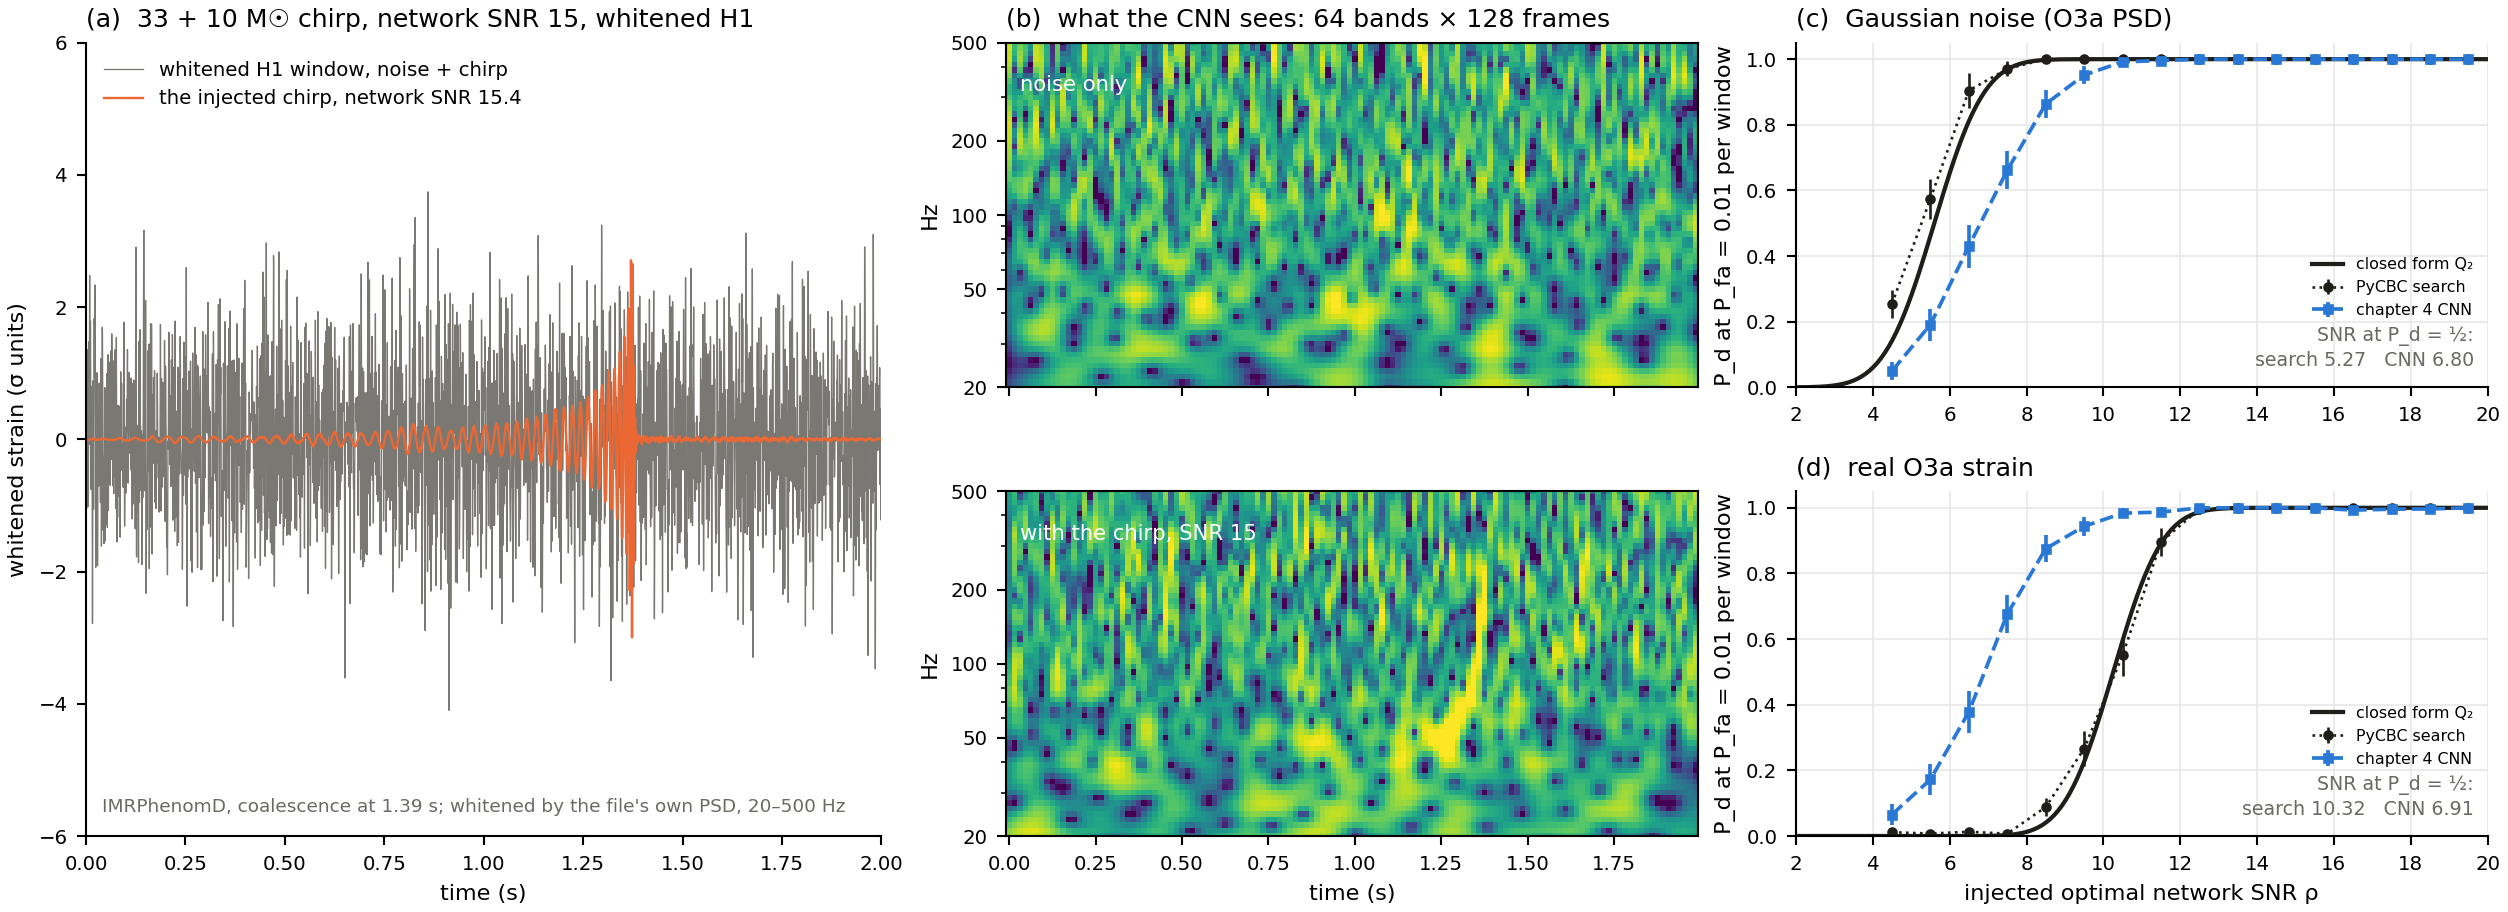
\includegraphics[width=\textwidth]{demos/gw_detect.png}
\caption{A chapter-4 CNN against the matched filter on LIGO strain. (a) A
whitened $2$\,s H1 window from the validation set with its injected
$33 + 10\,M_\odot$ chirp at network SNR 15. (b) The two spectrograms the
network must tell apart. (c) Detection probability against injected SNR in
Gaussian noise at $10^{-2}$ false alarms per window: the closed form at the
search's threshold, PyCBC's matched filter on the same windows with the two
detectors summed in quadrature, and the CNN. (d) The same on real O3a
strain, where glitches move the filter's threshold from $5.9$ to $10.4$ and
the CNN's barely at all. The CNN drawn in
each panel is the arm trained on the noise that panel tests it in.}
\label{fig:gw_detect}
\end{figure}

\paragraph{A CNN against the matched filter on LIGO strain.} This demo
has a theorem for a ceiling the way Leduc poker has its best response
(\S\ref{sec:game_leduc}) and the Boltzmann generator has quadrature. Advanced LIGO's strain
is a time series at audio rates, and a binary-black-hole merger is a chirp
that sweeps from 25 to a few hundred Hz in under a second. The Gravitational
Wave Open Science Center publishes every observing run under CC BY 4.0
(Abbott et al.\ 2023, \href{https://doi.org/10.3847/1538-4365/acdc9f}{ApJS 267,
29}); real events are too few to train on, so the training set is real
detector noise with simulated chirps injected at chosen signal-to-noise
ratios. The detector to beat is the matched filter: in stationary Gaussian
noise, for a signal whose waveform and arrival time are known, it is the
Neyman--Pearson optimum, and its detection probability at threshold
$\rho^\ast$ for a signal of optimal SNR $\rho$ is a Marcum $Q$-function.
Three things change relative to the CIFAR demo:

\begin{itemize}
  \item \textbf{The data is real detector noise with the signal we chose.}
    Twenty-six file pairs of O3a strain from H1 and L1, science-mode and free
    of hardware injections, cut into $2$\,s windows and whitened by each
    file's own median-Welch PSD over 20--500\,Hz. Half the training windows and a third of the validation windows carry an
    IMRPhenomD chirp from PyCBC, masses uniform in $[10, 50]\,M_\odot$, random
    sky position, projected onto both detectors and scaled to a network SNR
    uniform in $[4, 20]$. Two noise sets share every window and every
    injection: Gaussian noise coloured by the same PSD, the theorem's regime,
    and the strain itself. $40{,}760$ training and $12{,}228$ validation
    windows.
  \item \textbf{The instrument is a closed form, and the filter is checked
    against it first.} PyCBC's matched filter with the injected template, at
    the known arrival time, reproduces $Q_1(\rho, \rho^\ast)$ on the Gaussian
    set to within binomial error in every SNR bin --- the SNR at half
    detection is $4.68$ against the theorem's $4.75$ for H1 at a false-alarm
    rate of $10^{-2}$ per window --- so the injection's SNR and the whitening
    agree on one PSD. The search statistic then adds the two detectors'
    filter outputs in quadrature and maximises over the window and the
    $\pm 10$\,ms inter-detector delay, as a search must, and the CNN, which
    sees no time, is compared to that.
  \item \textbf{The network is Chapter~\ref{chap:bn}'s CIFAR net.}
    \texttt{CIFAR-CNN8-wide-BN}: eight convolutions in four conv-conv-pool
    stages at 16, 16, 32, 32 channels into the $2 \times 512$ head. The two
    edits are the two-channel stem and the two-way output, $0.83$\,M
    parameters at this input. The input is a
    $2 \times 64 \times 128$ image, each channel a constant-Q spectrogram
    of one detector's whitened window (64 log-spaced bands over
    20--500\,Hz, 128 frames); the ordinary train step with integer labels,
    Adam at $10^{-3}$ with one warm-up epoch and cosine decay, batch 64,
    six epochs, under two minutes on one card. Nothing in the codegen
    moved. The BatchNorm is the batch-statistics form of that chapter's
    headline rows, scored here on each test batch's own statistics rather
    than running ones; the sign-language, leaf and band demos inherit the
    same net.
\end{itemize}

\paragraph{Scored against the theorem.} Detection probability by injected
network SNR on the Gaussian set, $12{,}228$ validation windows, every
threshold set on the $8{,}177$ noise-only windows so that one in a hundred
exceeds it. The last column of Table~\ref{tab:gw_gaussian} is the SNR at which
each row crosses one half.

\begin{table}[H]
\centering
\caption{Detection probability by injected SNR in Gaussian noise, at a false-alarm rate of $10^{-2}$.}
\label{tab:gw_gaussian}
\small
\begin{tabular}{@{}l r r r r r r r r r@{}}
\hline
$\rho$ & 4 & 5 & 6 & 7 & 8 & 9 & 10 & 12 & $\rho_{1/2}$ \\
\hline
closed form $Q_2(\rho, \rho^\ast)$, $\rho^\ast = 5.86$ & $0.14$ & $0.46$ & $0.80$ & $0.96$ & $1.00$ & $1.00$ & $1.00$ & $1.00$ & $5.63$ \\
matched filter, quadrature sum, true template & $0.26$ & $0.58$ & $0.90$ & $0.97$ & $1.00$ & $1.00$ & $1.00$ & $1.00$ & $\mathbf{5.27}$ \\
CNN on spectrograms, trained on Gaussian noise & $0.05$ & $0.19$ & $0.43$ & $0.66$ & $0.86$ & $0.95$ & $0.99$ & $1.00$ & $6.80$ \\
random                                        & $0.01$ & $0.01$ & $0.01$ & $0.01$ & $0.01$ & $0.01$ & $0.01$ & $0.01$ & --- \\
\hline
\end{tabular}
\end{table}

\noindent The known-time filter sits on its closed form; the search, which
maximises over time, reaches half detection at $5.27$ against $Q_2$'s $5.63$
at the same threshold, because the maximum over the samples around an
arrival hands a signal a little SNR that the noise-only threshold never
sees. The CNN trails the search by $1.5$ units of SNR. Gabbard et al.\ 2018
(\href{https://doi.org/10.1103/PhysRevLett.120.141103}{PRL 120}) closed that
gap with a one-dimensional network on the whitened strain and ten times the
training set. One reading is that a log-power spectrogram discards the phase
the filter integrates; the demo did not test it, and this is the demo's
number, not the architecture's ceiling.

\paragraph{Real noise costs the filter, not the network.} LIGO noise is
neither stationary nor Gaussian, and the production search adds a $\chi^2$
veto for exactly that reason. Table~\ref{tab:gw_real} is the same rows on the
strain itself, with each model trained on one noise set and scored on both.

\begin{table}[H]
\centering
\caption{The SNR for half detection in Gaussian and in real LIGO noise, each model trained on one noise set and tested on both.}
\label{tab:gw_real}
\small
\begin{tabular}{@{}l r r r@{}}
\hline
 & \multicolumn{2}{c}{$\rho_{1/2}$ at $10^{-2}$} & $10^{-3}$ \\
trained on & tested on Gaussian & tested on real & tested on real \\
\hline
CNN, Gaussian noise         & $6.80$ & $7.17$ & $18.7$ \\
CNN, real O3a strain        & $6.65$ & $\mathbf{6.91}$ & $\mathbf{7.52}$ \\
matched filter, quadrature sum & $\mathbf{5.27}$ & $10.32$ & --- \\
\hline
\end{tabular}
\end{table}

\noindent The network trained on real strain is the better one on both noise
sets, by $0.15$ in Gaussian noise and $0.26$ in real; training in the
theorem's regime buys nothing even there. The filter loses five units of
SNR to glitches at $10^{-2}$, and at
$10^{-3}$ its threshold is $417$: eight validation windows hold a glitch
that loud, and without a veto the filter has no row. The network trained on
Gaussian noise needs an SNR of $19$ there; the one trained on real strain
still reaches half detection at $7.5$. Training on the real detector is what
teaches the glitch tail.

\subsection*{WaveNet (\texttt{Bestiary/WaveNet.lean})}
\emph{One} new primitive (Definition~\ref{layer:waveNetBlock}). Dilated causal
convolutions for raw audio sample prediction (van den Oord et al.\
2016, \href{https://arxiv.org/abs/1609.03499}{arXiv:1609.03499}): exponential receptive field, linear parameter
growth. The foundation of neural TTS and PixelCNN. Variants: single
stack (0.4M), 3-stack (paper setup, with a NetSpec-linearity
approximation), music (single stack, 4.1M), tiny. One honest
limitation: the residual-vs-skip dual-output pattern doesn't
linearize cleanly, so the 3-stack variant uses a simplified
channel-flow approximation.

\begin{verbatim}
def waveNet : NetSpec where
  name   := "WaveNet (single stack, speech)"
  imageH := 16000                                 -- 1 second @ 16 kHz
  imageW := 1
  layers := [
    -- Input embedding: 256 mu-law bins → 32 residual channels
    .conv2d 256 32 1 .same .identity,
    -- One stack of 10 dilated residual blocks (dilations 2⁰..2⁹)
    .waveNetBlock 32 512 10,
    -- Output head: skip-sum → 1×1 → 1×1, 256-way categorical
    .conv2d 512 256 1 .same .relu,
    .conv2d 256 256 1 .same .identity
  ]
\end{verbatim}

\subsection*{Whisper (\texttt{Bestiary/Whisper.lean})}
\emph{One} new primitive (Definition~\ref{layer:transformerDecoder}). Encoder-decoder transformer over log-mel
spectrograms (Radford et al.\ 2022,
\href{https://arxiv.org/abs/2212.04356}{arXiv:2212.04356}). Encoder is
\texttt{.transformerEncoder} on the 1500 post-stem audio tokens;
decoder is \texttt{.transformerDecoder} (from DETR) with
\texttt{nQueries = 0} --- a clean seq2seq decoder with self-attn +
cross-attn + FFN, text tokens coming from a separate
\texttt{.dense vocab$\to$D} stand-in tied to the LM head. Variants:
tiny (7M enc, paper 39M total), base (19M enc, paper 74M), small
(85M enc + 153M dec+emb = 238M vs paper 244M), medium (302M enc,
paper 769M), large (629M enc, paper 1.55B total), plus a shared
decoder spec and tinyWhisper fixture. Encoder and decoder share width
and depth per variant, and the paper totals are encoder, decoder and the
tied token embedding together (small: $85 + 153 = 238$M against 244M). The multitask interface (swap a prefix token to change
language or switch between transcribe / translate) is
prompt-engineering, not architecture --- Whisper's architectural
novelty is essentially zero.

\begin{verbatim}
def whisperSmall : NetSpec where
  name   := "Whisper small encoder"
  imageH := 1500                                  -- post-stem audio tokens (3000 / 2)
  imageW := 1
  layers := [
    -- 12 encoder blocks, dim 768, 12 heads, mlp 3072
    .transformerEncoder 768 12 3072 12
  ]
\end{verbatim}

\section{Beyond vision --- demo: neural quantum states on the Ising chain}
\label{sec:bestiary_beyond}

Architectures where the task domain is neither a 2D image nor a token
sequence: a wavefunction, a radiance field, a shared embedding space.
The demo points Chapter~\ref{chap:attention}'s transformer, as an
encoder and as a decoder, at a quantum ground state, where there is no
dataset at all and the ceiling is a solved model; the entries after it
(NeRF, CLIP, LLaVA) make the same point from the other side
--- several have essentially no architectural novelty, and the interesting
work lives in the data, loss, or training procedure.

\paragraph{A transformer as a wavefunction.} Take a ring of $N$ spins, each
up or down. Neighbours want to agree, with strength $J$; a field $h$ wants
each spin to point sideways, which in quantum mechanics means to be up and
down at once. That is the transverse-field Ising chain,
$H = -J \sum_i \sigma^z_i \sigma^z_{i+1} - h \sum_i \sigma^x_i$, and its
lowest-energy state is the textbook quantum phase transition: for $h < J$
the spins agree, for $h > J$ they do not, and at $h = J$ every pattern in
between. The ground state is a probability amplitude $\psi(\sigma)$ over
all $2^N$ configurations, and a \emph{neural quantum state} (Carleo \&
Troyer 2017, \href{https://doi.org/10.1126/science.aag2302}{Science 355,
602}) is a network that maps a configuration $\sigma \in \{\pm 1\}^N$ to
its log-amplitude, trained by lowering the energy
$\langle \psi | H | \psi \rangle / \langle \psi | \psi \rangle$. The demo
climbs a ladder of three such networks, each written as a closed-form
reference times a learned residual, $\psi_\theta = \psi_{\mathrm{ref}}
\cdot \exp f_\theta$, with $\psi_{\mathrm{ref}}$ the mean-field product
state at its optimal angle --- a log-amplitude linear in $\sigma$ that the
host adds to the network's output before any ratio is formed. $f_\theta$ is
an MLP on the $\pm 1$ spins ($5{,}057$ parameters at $N = 12$); a ViT that
reads patches of $p$ spins as token ids through
\texttt{tokenPositionEmbed}, two encoder blocks at $d = 32$, a mean over
tokens and a one-unit head ($25{,}825$; the transformer wavefunctions of
Viteritti, Rende \& Becca 2023,
\href{https://arxiv.org/abs/2211.05504}{arXiv:2211.05504}); or a GPT on
the same tokens, two causal blocks and an \texttt{lmHead}, whose
conditionals are the wavefunction, $|\psi(\sigma)|^2 = \prod_k
p(\mathrm{patch}_k \mid \mathrm{patch}_{<k})$, so that a sample is an
autoregressive draw through the TinyGPT sampling loop with a vocabulary of
$2^p$ ($25{,}956$; Sharir et al.\ 2020,
\href{https://arxiv.org/abs/1902.04057}{arXiv:1902.04057}). Three things
change relative to the TinyGPT demo:

\begin{itemize}
  \item \textbf{There is no dataset.} The training signal is the model's
    own local energies, $E_{\mathrm{loc}}(\sigma) = -J \sum_i \sigma_i
    \sigma_{i+1} - h \sum_i \psi(\sigma^{(i)}) / \psi(\sigma)$ with
    $\sigma^{(i)}$ the $i$-th spin flipped, so a batch of $B$ configurations
    costs one extra forward at batch $B \cdot N$. The energy is a weighted
    mean of $E_{\mathrm{loc}}$ and its gradient, $\partial_\theta E =
    2 \sum_\sigma p_\sigma \,(E_{\mathrm{loc}}(\sigma) - E)\,
    \partial_\theta \log \psi(\sigma)$, is one host weight $w_\sigma$ per
    configuration. That weight enters the train step through the rank-2
    squared-error block of the diffusion demo
    (\S~\ref{sec:bestiary_diffusion}) with the target set to
    $\mathrm{out} - M w / 2$, so the block's output cotangent is exactly
    $w$: the Pong DQN's trick (\S~\ref{sec:game_pong}) with a
    physical target, and zero new codegen. At $N = 12$ the sum runs over all
    $4{,}096$ configurations and the gradient is exact; at $N = 64$ the MLP
    and ViT sample by Metropolis on $1{,}024$ chains and the GPT draws
    independent samples.
  \item \textbf{Structure first, the network models the rest.} At
    $f_\theta = 0$ the ansatz is the mean-field state, so step 0 of every
    run prints the mean-field energy to six digits and the network only has
    to learn what mean field gets wrong. For the MLP and ViT the reference
    is a fixed visible bias; for the GPT it is a fixed bias on the logits,
    so that the conditionals stay normalised.
  \item \textbf{The instrument is a solved model.} Every number in
    Table~\ref{tab:nqs_ladder} is bracketed by a closed form: enumeration of the $4{,}096 \times 4{,}096$
    Hamiltonian at $N = 12$, and at $N = 64$ the free-fermion solution of
    Pfeuty 1970, which agrees with enumeration to $7 \times 10^{-15}$ where
    both apply. The variance of $E_{\mathrm{loc}}$ over the samples is the
    instrument that needs no ceiling: zero for an eigenstate at any $N$.
\end{itemize}

Figure~\ref{fig:nqs_ising} is the chain's three phases as the network draws
them, and the check against the exact ground state.

\begin{figure}[H]
\centering
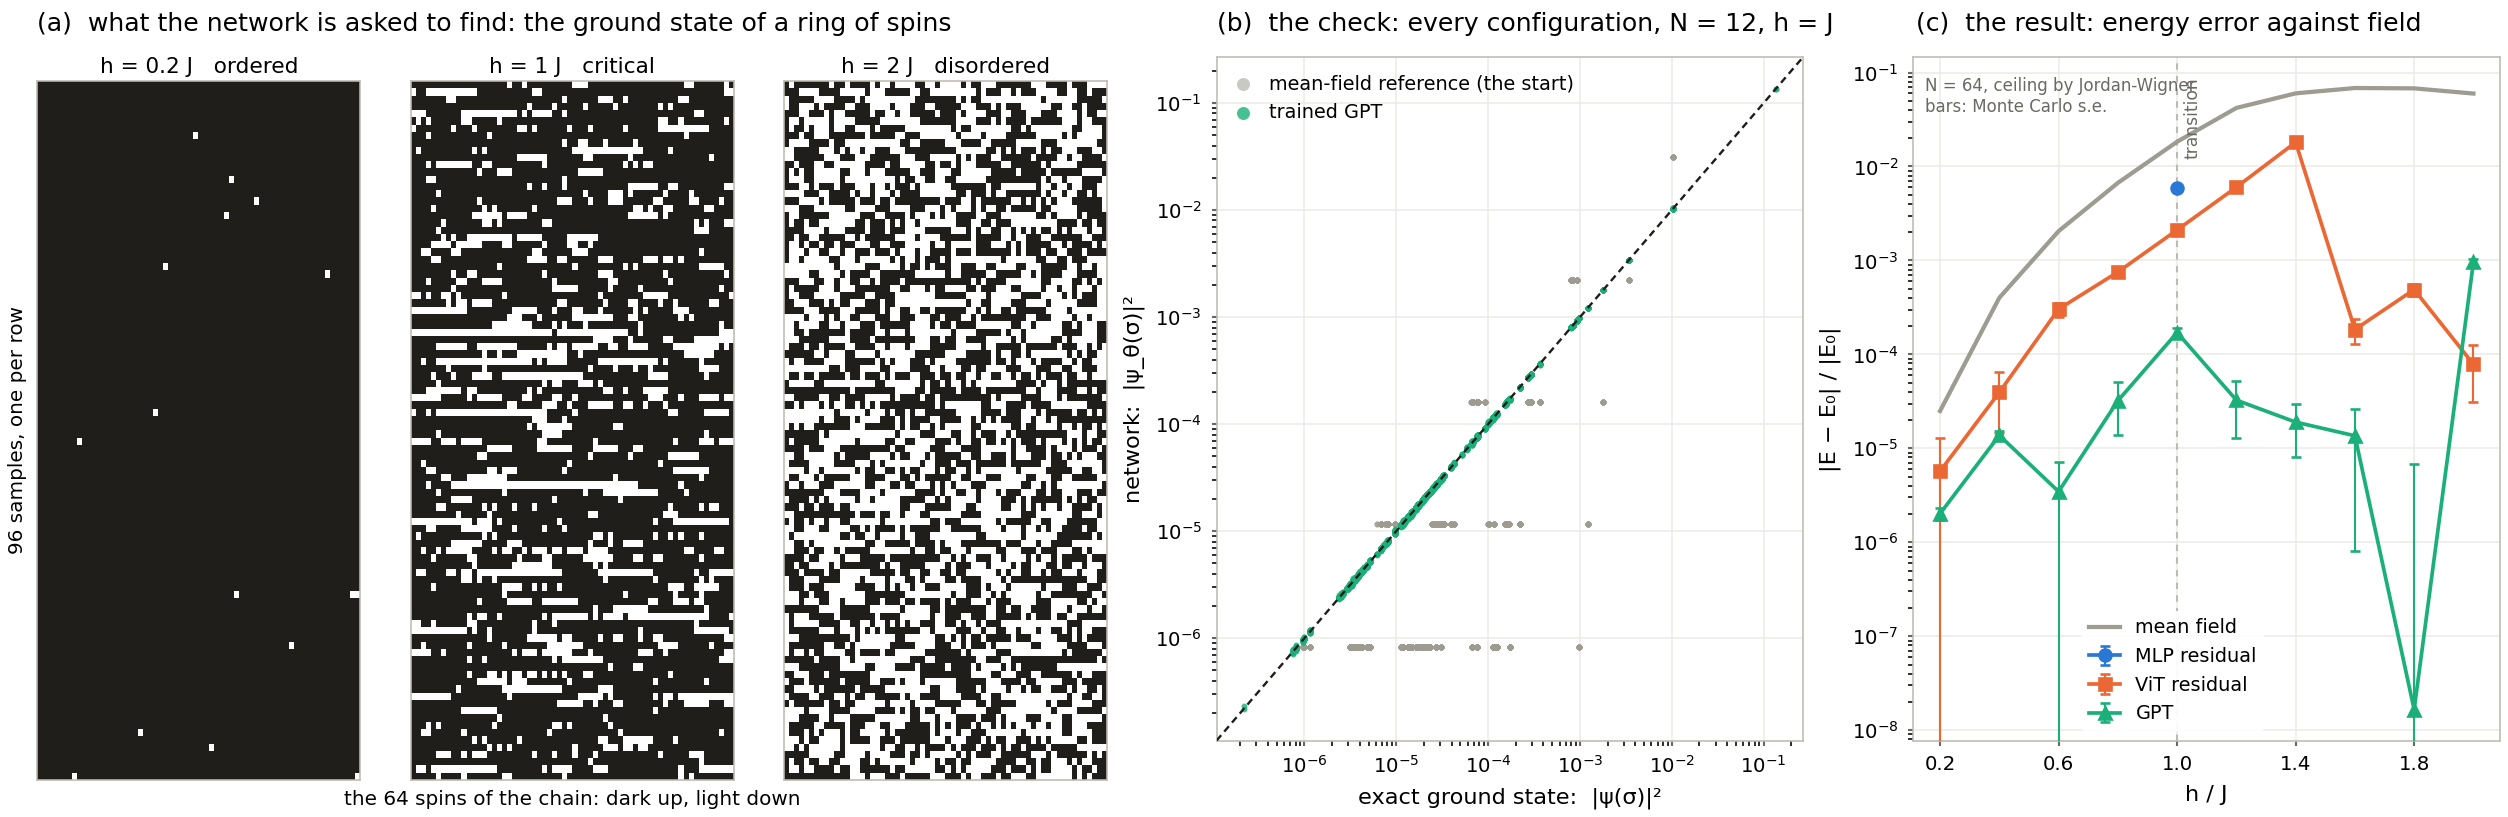
\includegraphics[width=\textwidth]{demos/nqs_ising.png}
\caption{Neural quantum states on the transverse-field Ising chain. (a)
What the network is asked to find. Each row is one configuration of the
64-spin ring drawn from the trained GPT wavefunction, dark for up and light
for down: at $h = 0.2J$ the spins agree, at $h = J$ they form domains of
every size, at $h = 2J$ they are nearly independent. (b) The check. For
every one of the $4{,}096$ configurations at $N = 12$, $h = J$, the
probability the trained GPT assigns against the exact ground state's; in
grey, the mean-field reference the network starts from, which is a product
state and wrong by orders of magnitude in the tails. (c) The result.
Relative energy error against $h/J$ at $N = 64$ for the three networks,
the mean-field floor in grey, bars the Monte Carlo standard error of the
sample energy.}
\label{fig:nqs_ising}
\end{figure}

\paragraph{The ladder at the critical point.} $h = J$, Adam with cosine
decay, $4{,}000$ steps at $N = 12$ and $2{,}000$ at $N = 64$, one RTX 4060
Ti: 50\,s to 330\,s per row at $N = 12$ with the XLA compile included and
about twenty minutes at $N = 64$. The $N = 64$ energies are means over the
final $8{,}192$ samples, whose Monte Carlo standard error is four to five
percent of the MLP and ViT entries and eleven percent of the GPT's.
Table~\ref{tab:nqs_ladder} is the ladder.

\begin{table}[H]
\centering
\caption{Neural quantum states on the transverse-field Ising chain at the critical point, at $N = 12$ and $N = 64$.}
\label{tab:nqs_ladder}
\small
\begin{tabular}{@{}l r r r r r@{}}
\hline
$h = J$ & params & $(E - E_0)/|E_0|$ & $\mathrm{Var}(E_{\mathrm{loc}})$ & $\langle \sigma^x \rangle$ & $\langle \sigma^z_1 \sigma^z_{1+N/2} \rangle$ \\
\hline
\multicolumn{6}{@{}l}{\textit{$N = 12$, exact gradient by enumeration}} \\
mean field (floor)       & 0          & $2.1 \times 10^{-2}$ & $0.75$ & 0.5000 & 0.7500 \\
MLP residual             & $5{,}057$  & $1.6 \times 10^{-5}$ & $4.3 \times 10^{-3}$ & 0.6383 & 0.4613 \\
ViT residual             & $25{,}825$ & $1.5 \times 10^{-5}$ & $2.5 \times 10^{-3}$ & 0.6381 & 0.4618 \\
GPT                      & $25{,}956$ & $\mathbf{3.3 \times 10^{-6}}$ & $5.2 \times 10^{-4}$ & 0.6384 & 0.4611 \\
exact (enumeration)      & ---        & 0 & 0 & 0.6384 & 0.4610 \\
\hline
\multicolumn{6}{@{}l}{\textit{$N = 64$, $p = 4$, $1{,}024$ chains}} \\
mean field (floor)       & 0          & $1.8 \times 10^{-2}$ & $4.0$ & 0.5000 & 0.7500 \\
MLP residual, Metropolis & $8{,}385$  & $5.9 \times 10^{-3}$ & $3.7$ & 0.5660 & 0.6256 \\
ViT residual, Metropolis & $26{,}529$ & $2.1 \times 10^{-3}$ & $0.48$ & 0.5921 & 0.5616 \\
GPT, exact sampling      & $27{,}056$ & $\mathbf{1.7 \times 10^{-4}}$ & $0.020$ & 0.6341 & 0.3498 \\
exact (Jordan--Wigner)   & ---        & 0 & 0 & 0.6367 & 0.3036 \\
\hline
\end{tabular}
\end{table}

\noindent At $N = 12$ every rung sits three to four orders below the floor
and the GPT, whose conditionals are the wavefunction, is the best of them
at every field in the sweep. At $N = 64$ the ladder separates, and the
sampler is why: the GPT's draws are independent and its gradient noise is
only the batch's, so it sits below $4 \times 10^{-5}$ at eight of the ten
fields; the exceptions are the critical point, $1.7 \times 10^{-4}$, and
$h = 2J$, $9.6 \times 10^{-4}$, where the sweep's learning rate plateaued
(a third of the rate for twice the steps reaches $10^{-6}$). The ViT on
Metropolis chains is worse at every field but $h = 2J$, by three times at
$h \le 0.4J$ and by ten to a thousand from $0.6J$ to $1.8J$, at the same
parameter count and step budget, and at $h = 1.4J$ doubling its chains and
steps makes it diverge. That is the regime
stochastic reconfiguration (Sorella 1998,
\href{https://doi.org/10.1103/PhysRevLett.80.4558}{PRL 80, 4558}) exists
for; nothing at $N = 12$ needed it.

\paragraph{Three things the sweep taught.} The reference decides the
small-field rows, and the ablation says by how much: the same ViT, from
the uniform state and from the mean-field state, is three orders of
magnitude apart at $h = 0.2J$ ($3.0 \times 10^{-5}$ against
$1.6 \times 10^{-8}$), two at $0.4J$, and level at $h = J$, where the
reference is as wrong as the uniform state and the network does all the
work either way. Low variance with a wrong energy is the wrong state: the
ViT at $N = 12$, $h = 0.8J$ converges to $5.4 \times 10^{-4}$ with a
variance of $1.1 \times 10^{-3}$, a third of the MLP's at the same field,
unmoved by seeds, steps,
width, depth or patch size, and its excess energy is $\Delta/2$ to three
digits, $\Delta$ the splitting between the even- and odd-parity states ---
it converged to the symmetry-broken half of the finite-$N$ cat state that
the product-state reference imprints, and the fix was more structure, not
more network: the symmetrised reference $\psi_{\mathrm{MF}}(\sigma) +
\psi_{\mathrm{MF}}(-\sigma)$, one \texttt{logaddexp} on the host, takes it
to $2.0 \times 10^{-5}$. And signs are the open row. The Ising ground state
is positive, so the rungs above are real; the $J_1$--$J_2$ Heisenberg chain
is frustrated and its ground state has a sign structure, so the head gets a
second slot, $(\log|\psi|, \varphi)$, with Marshall's sign rule as the
reference phase and two host weights per configuration through the same
block. At $N = 16$ the phase head learns the Marshall signs from scratch at
$J_2 = 0$ (fidelity $0.9985$), every arm finds the Majumdar--Ghosh dimer
state at $J_2 = J_1/2$ to $3 \times 10^{-6}$ with fidelity $1.000$, and past
that point, where the rule breaks, every arm stalls at $10^{-2}$ with a
fidelity below $0.6$ that four times the width and twice the steps move
only to $0.58$.

Two gates sit under the table. The autoregressive sampler,
drawn $16{,}384$ times from a trained $N = 12$ state and scored by table
lookup, lands within $0.1$ standard errors of the same state's enumerated
energy; on a trained state a single check scatters wider than $N(0, 1)$
because $E_{\mathrm{loc}}$ is heavy-tailed, so the pooled test over eight
draw seeds is the one that decides. And step 0 of every run is the floor
row to six digits, which is the check that the host adds the reference
where the ansatz says it does. The trainer is
\texttt{demos/MainNqsIsing.lean}; the closed forms, the Lanczos ceiling ---
the exact ground state of the $J_1$--$J_2$ chain in its $S_z = 0$ sector,
$12{,}870$ states at $N = 16$, by Lanczos iteration, the $E_0$ that rung's
errors are measured from --- and every table are
\texttt{scripts/demos/\allowbreak nqs\_metrics.py}.

\subsection*{NeRF (\texttt{Bestiary/NeRF.lean})}
\emph{Two} new primitives (Definition~\ref{layer:positionalEncoding},
Definition~\ref{layer:nerfMLP}). The "it's literally just an MLP" paper
(Mildenhall et al.\ 2020,
\href{https://arxiv.org/abs/2003.08934}{arXiv:2003.08934}). Under 600K params at canonical
config; the architectural novelty is nonexistent. What makes NeRF work
is the positional encoding + the volumetric-rendering loss ---
both outside the network, not layers in it. Variants:
canonical (593K), fast (167K hidden=128), tiny fixture.

\begin{verbatim}
def nerf : NetSpec where
  name   := "NeRF (canonical)"
  imageH := 1
  imageW := 1
  layers := [
    -- Positional encoding of (x,y,z): 3 coords × 2 × 10 freqs = 60-dim
    .positionalEncoding 3 10,
    -- 8-layer MLP with mid-skip + dual density/RGB heads.
    -- encodedDirDim = 3·2·4 = 24 (3D view direction, 4 frequencies)
    .nerfMLP 60 24 256
  ]
\end{verbatim}

\subsection*{CLIP (\texttt{Bestiary/CLIP.lean})}
\emph{Zero} new primitives. Two textbook encoders glued together by a
contrastive loss (Radford et al.\ 2021,
\href{https://arxiv.org/abs/2103.00020}{arXiv:2103.00020}): a ResNet-50 or ViT-B for images, a 12-layer causal
transformer for text, each with a final linear projection to a shared
embedding space. Variants: CLIP-RN50, CLIP-ViT-B/32 (151M, paper-exact),
CLIP-ViT-L/14 (427M, paper-exact), tiny fixture. The architectural
lesson from CLIP is identical to NeRF's: what is new is the data and the
objective, not a layer.

\begin{verbatim}
def clipViTB32ImageEncoder : NetSpec where
  name   := "CLIP-ViT-B/32 (image encoder)"
  imageH := 224
  imageW := 224
  layers := [
    -- ViT-B/32: patch size 32 → 49 patches, dim 768, 12 blocks, 12 heads
    .patchEmbed 3 768 32 49,
    .transformerEncoder 768 12 3072 12,
    -- [CLS] token → shared 512-dim embedding space
    .dense 768 512 .identity
  ]
\end{verbatim}

\subsection*{LLaVA / LLaVA-1.5 (\texttt{Bestiary/LLaVA.lean})}
\emph{Zero} new primitives. The cleanest exhibit of the modern
vision-language pattern (Liu et al.\ 2023,
\href{https://arxiv.org/abs/2304.08485}{arXiv:2304.08485}; LLaVA-1.5:
\href{https://arxiv.org/abs/2310.03744}{arXiv:2310.03744}): frozen CLIP ViT encoder + small MLP
projector + (mostly) frozen LLaMA/Vicuna language model. Trained in
two stages --- projector-only pretrain, then joint instruction fine-
tune. Shown as separate NetSpecs per component: vision encoder
(303M, matching CLIP ViT-L/14), LLaVA-1 single-linear projector
(4M), LLaVA-1.5 two-layer MLP projector (21M), LLM backbones at 7B
and 13B. The LLM specs undercount real LLaMA by $\sim$23\% because
our \texttt{.transformerEncoder} uses a standard 2-projection FFN
while LLaMA uses SwiGLU (3 projections); depth / width / heads still
match. Key ratio: the projector is \textbf{0.3\%} of total LLaVA-1.5
7B parameters --- the entire interesting work of the model lives in
~21M of trainable bolt-on between two pretrained backbones. BLIP-2,
Flamingo, and every modern VLM demo generalize this template with
fancier adapters (Q-Former, Perceiver resampler, gated xattn-dense),
but the frozen-backbone-plus-adapter shape is the same.

\begin{verbatim}
def llava15Projector : NetSpec where
  name   := "LLaVA-1.5 projector (2-layer MLP)"
  imageH := 576                                   -- visual token count (24×24)
  imageW := 1
  layers := [
    -- The entire LLaVA architectural contribution: map CLIP's 1024-dim
    -- image tokens into the LLM's 4096-dim embedding space. ~21M params
    -- — roughly 0.3% of total LLaVA-1.5 7B. GELU between is zero-param.
    .dense 1024 4096 .identity,
    .dense 4096 4096 .identity
  ]
\end{verbatim}

\section{Structure --- demo: a distogram ResNet against the CASP16 field}
\label{sec:bestiary_structure}

Networks whose input is a protein's sequence and whose output is its
shape. The demo is the recipe that held the field from 2018 to 2020 --- a
deep two-dimensional residual network predicting a histogram of distances
for every pair of residues, and a fold obtained by descending that
histogram's negative log-likelihood --- with a frozen protein language
model in place of the multiple-sequence alignment those methods read,
scored on CASP16's targets beside the groups that predicted them blind.
The \bestiaryref{bestiary:evoformer}{Evoformer entry} that closes the section is
the architecture that ended that era.

\paragraph{A residual network on residue pairs.} A protein is a string
over twenty letters, and its fold is set by which residues end up near
each other. Write the distance between the $\beta$-carbons of residues $i$
and $j$ as a histogram over 64 bins from 2 to 22\,Å, one per pair:
that $L \times L$ array of histograms is the \emph{distogram}, and
AlphaFold~1 (Senior et al.\ 2020,
\href{https://doi.org/10.1038/s41586-019-1923-7}{Nature 577, 706}) and
trRosetta (Yang et al.\ 2020,
\href{https://doi.org/10.1073/pnas.1914677117}{PNAS 117, 1496}) were
exactly this shape: per-residue features tiled into an $L \times L$ pair
tensor, a deep 2D ResNet, a histogram per pair, and a fold by gradient
descent on the histogram's negative log-likelihood over coordinates. Those
methods read a multiple-sequence alignment; here the per-residue features
are the final-layer representation of ESM-2 (Lin et al.\ 2023,
\href{https://doi.org/10.1126/science.ade2574}{Science 379, 1123}), a
protein language model trained on sequences alone, frozen, $2{,}560$ wide
at its 3B-parameter size, with the model's own contact map --- a logistic
regression on its attention heads --- riding along as one pair channel.
The input is a single sequence, and the language model runs once, outside
the proof. The network is Chapter~\ref{chap:residual}'s ResNet with its strides
removed --- sixteen of its basic blocks at 128 channels,
\texttt{residualBlock 128 128 16 1} --- with one new layer in front (the pair
tile, Definition~\ref{layer:pairTile}: two dense maps and an outer sum) and a
$1 \times 1$ head of 132 channels --- the 66-class distance head, which is
the 64 bins, a ``beyond 22\,Å'' class and an ``unobserved'' class at
weight zero, how a missing residue leaves the loss, and trRosetta's three
orientation heads, the dihedrals $\omega$ and $\theta$ and the angle
$\varphi$ between the two residues' $\mathrm{C}_\alpha$--$\mathrm{C}_\beta$
bonds in $15^\circ$ bins. $5{,}418{,}244$ parameters. Training reads every
protein chain the PDB released before CASP16 opened on 2024-05-01, one
representative per 40\,\% sequence cluster, $26{,}310$ chains, as random
$96 \times 96$ windows of their pair maps, 100 epochs in 21 hours on one
RTX 4060 Ti; inference tiles the same window over a target at stride 32
and averages the logits, so the trained artifact is the one that is
scored. The fold is Adam on the smoothed negative log-likelihood of the
predicted distances and angles over one pseudo-$\mathrm{C}_\beta$ point
per residue, with a chain term and a clash term, from a classical-MDS
start, in both mirror images. Three things change relative to the
segmentation demo:

\begin{itemize}
  \item \textbf{The input is a pair map built on the host from a frozen
    model's output.} The pair tile takes the two residue blocks of a crop,
    $2 L D$ numbers per example, projects each through its own
    $D \to C$ map and outer-sums them into the $[C, L, L]$ map; $K$ host
    pair planes are concatenated behind the tile's channels. It is the one
    new layer and the one new proof item,
    \texttt{Proofs/Foundation/\allowbreak PairTile.lean}: the backward in each weight is the cotangent summed over the broadcast
    axis, then contracted with the block --- the two \texttt{reduce} +
    \texttt{dot\_general} pairs the emitter writes --- and there is no
    input gradient, because the blocks are the language model's and it is
    not trained. Everything downstream of the tile is the chapter's; the
    demo's gradient evidence is the finite-difference check on the tile's
    weights and the eval $\equiv$ train identity, not a whole-net step tie.
  \item \textbf{The loss has four heads and the label is packed.}
    \texttt{perPixelMultiCE} is the segmentation demo's weighted per-pixel
    cross-entropy summed over $K$ heads of one output tensor, the $K$
    labels carried mixed-radix in the one \texttt{int32} plane the
    segmentation ABI already passes, each head's ``unobserved'' class at
    weight zero. One sentence the fold needs: lDDT is a distance score and
    cannot see a mirror image, TM-score superposes with a proper rotation
    and can, and a fold from distances alone has that ambiguity --- the
    true trace of T1235-D1 and its mirror both score a $\mathrm{C}_\beta$-lDDT of 1.00, at
    TM-scores of 1.00 and 0.34. The $\omega$ dihedral is chiral, so with
    the orientation heads the hand is the lower-energy one.
  \item \textbf{The instrument is the field.} CASP16's Phase-1 targets ---
    84 evaluation units whose experimental structures were released after
    the predictions were in --- scored the way CASP scored them:
    OpenStructure's lDDT and US-align's TM-score reproduce the official
    table to the printed digit on nine field models, and our fold and
    every group's model are reduced to the same pseudo-$\mathrm{C}_\beta$
    atom before they are compared. The training set is the information the
    field had, a date cut; purging the 82 chains homologous to a target is
    an ablation, not the protocol, and at 64 channels it moves precision by
    less than a second seed does ($0.585 \to 0.599$, against $0.597$ for the
    seed). The single-sequence reference is
    ESMFold, the same language model under the folding trunk its authors
    trained for it.
\end{itemize}

Figure~\ref{fig:casp16_distogram} is one target's contact map, predicted
against measured, and our fold beside the field's.

\begin{figure}[H]
\centering
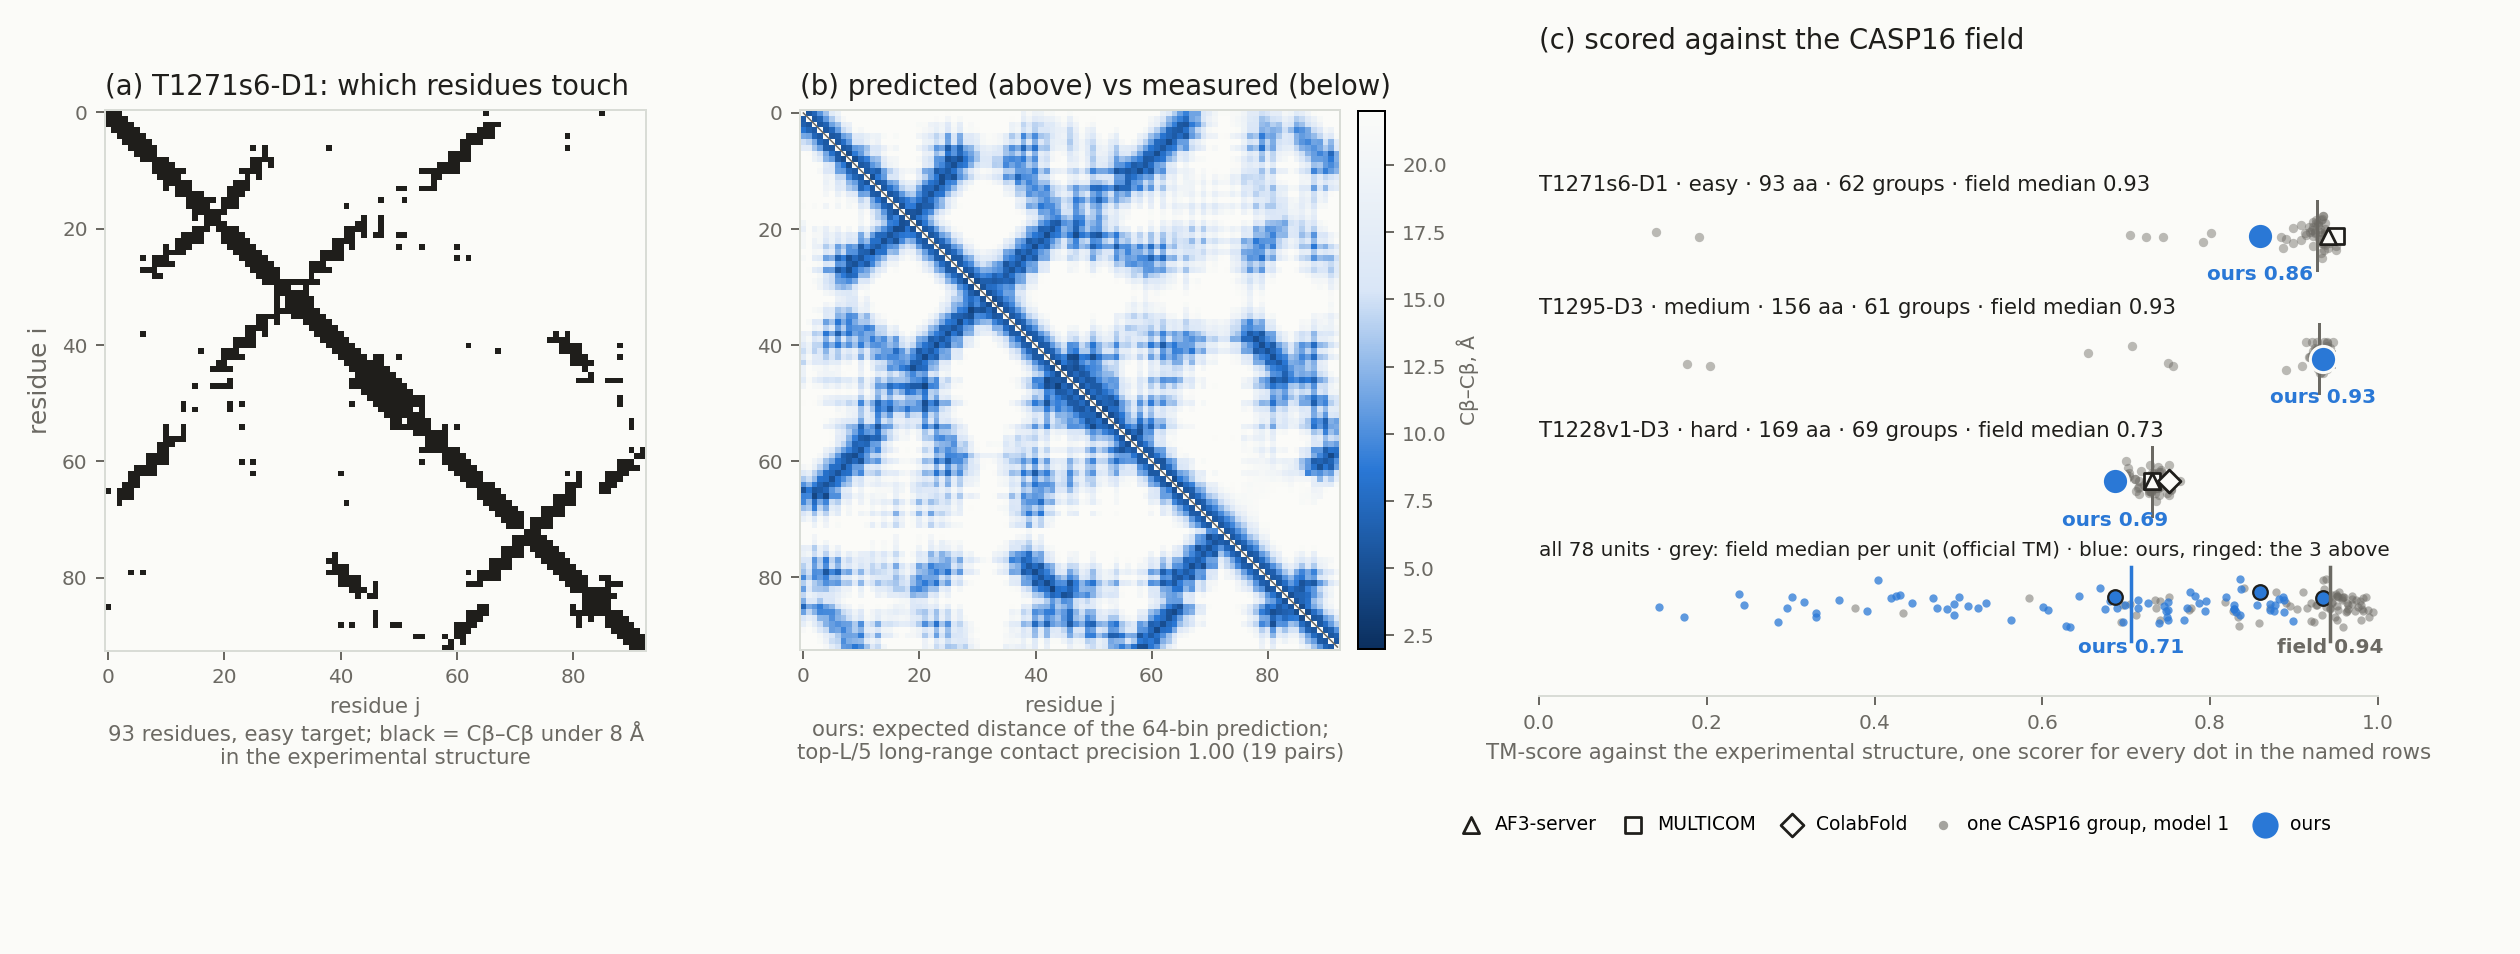
\includegraphics[width=\textwidth]{demos/casp16_distogram.png}
\caption{A distogram ResNet against the CASP16 field. (a) What the network
is asked to find: the contact map of T1271s6-D1, a 93-residue target,
black where two residues' $\beta$-carbons are within 8\,Å in the
experimental structure. (b) The check: the expected distance of the
predicted 64-bin histogram above the diagonal against the measured
distance below it; the top-$L/5$ long-range contacts are all right on this
unit. (c) The result: the TM-score of our fold on the three featured units
beside every CASP16 group's first model, AF3-server, MULTICOM and ColabFold
marked, and in the last row all 78 units, ours against the field's median
model per unit.}
\label{fig:casp16_distogram}
\end{figure}

\paragraph{The bracket on the CASP16 targets.} Table~\ref{tab:casp16_arms} is
the top-$L/5$ long-range contact precision over the 84 evaluation units (a long-range pair is 24 or
more residues apart; the number is the fraction of the $L/5$ most confident
such pairs that are within 8\,Å), the recall of the true long-range
contacts at $P > 0.5$, and the fold's $\mathrm{C}_\beta$-lDDT and TM-score over the 78
units the fold and the field both cover.

\begin{table}[H]
\centering
\caption{The distogram arms on the CASP16 targets: long-range contact precision and recall, $\mathrm{C}_\beta$-lDDT and TM-score.}
\label{tab:casp16_arms}
\small
\begin{tabular}{@{}l r r r r@{}}
\hline
arm & precision & recall & $\mathrm{C}_\beta$-lDDT & TM \\
\hline
one-hot residues, no language model, 64 ch         & 0.252 & 0.001 & 0.319 & 0.228 \\
ESM-2 3B's own contact head, nothing trained       & 0.759 &       &       &       \\
ESM-2 650M features, 64 ch, crop 64, 30 epochs     & 0.838 & 0.387 & 0.569 & 0.572 \\
the book run: 3B, its plane, 128 ch, crop 96, heads, 100 epochs & $\mathbf{0.873}$ & $\mathbf{0.476}$ & $\mathbf{0.627}$ & $\mathbf{0.646}$ \\
ESMFold v1: ESM-2 3B under its own trunk           &       &       & 0.751 & 0.778 \\
CASP16 field, the median first model per unit      &       &       &       & 0.892 \\
\hline
\end{tabular}
\end{table}

\noindent The language model is the lever and the ladder says by how much:
at 64 channels and 30 epochs the precision runs $0.585 \to 0.735 \to 0.838
\to 0.840$ from ESM-2's 35M to its 150M, 650M and 3B sizes, each model's
own contact head $0.474 \to 0.623 \to 0.754 \to 0.759$ beneath it, so the
network adds 0.08 to 0.11 on every language model and the ladder is flat
on precision past 650M, where the 3B step shows in the fold ($+0.012$). On
top of 650M each of width (128 channels), a 96-residue crop and the model's
contact map as a pair channel is worth $+0.01$ to $+0.02$ of precision and
the three add, the plane giving the hard class the most ($+0.09$ on its
own); with the 3B features they reach $0.880 / 0.622 / 0.632$ at 30
epochs, and the orientation heads cost 0.003 of precision and buy $+0.013$
of TM-score through the $\omega/\varphi$ restraints. The book run is that
configuration at 100 epochs, and the schedule bought nothing: against its
30-epoch twin ($0.877 / 0.628 / 0.645$) the paired differences over units
are $-0.004$, $-0.001$ and $+0.001$ with every 95\,\% interval across zero,
and validation precision is level from epoch 20. A second seed moves any
arm by at most 0.002 on any column, an ensemble of five arms does not beat
its best member, and the fold is converged: under its own potential the
experimental trace has higher energy than our fold on 78 of 78 units, the
map's own mean distances score an lDDT of 0.615 against the fold's 0.627,
and the two correlate at 0.90, so what the fold realises is the map.
Figure~\ref{fig:casp16_ablation} is what each lever buys.

\begin{figure}[H]
\centering
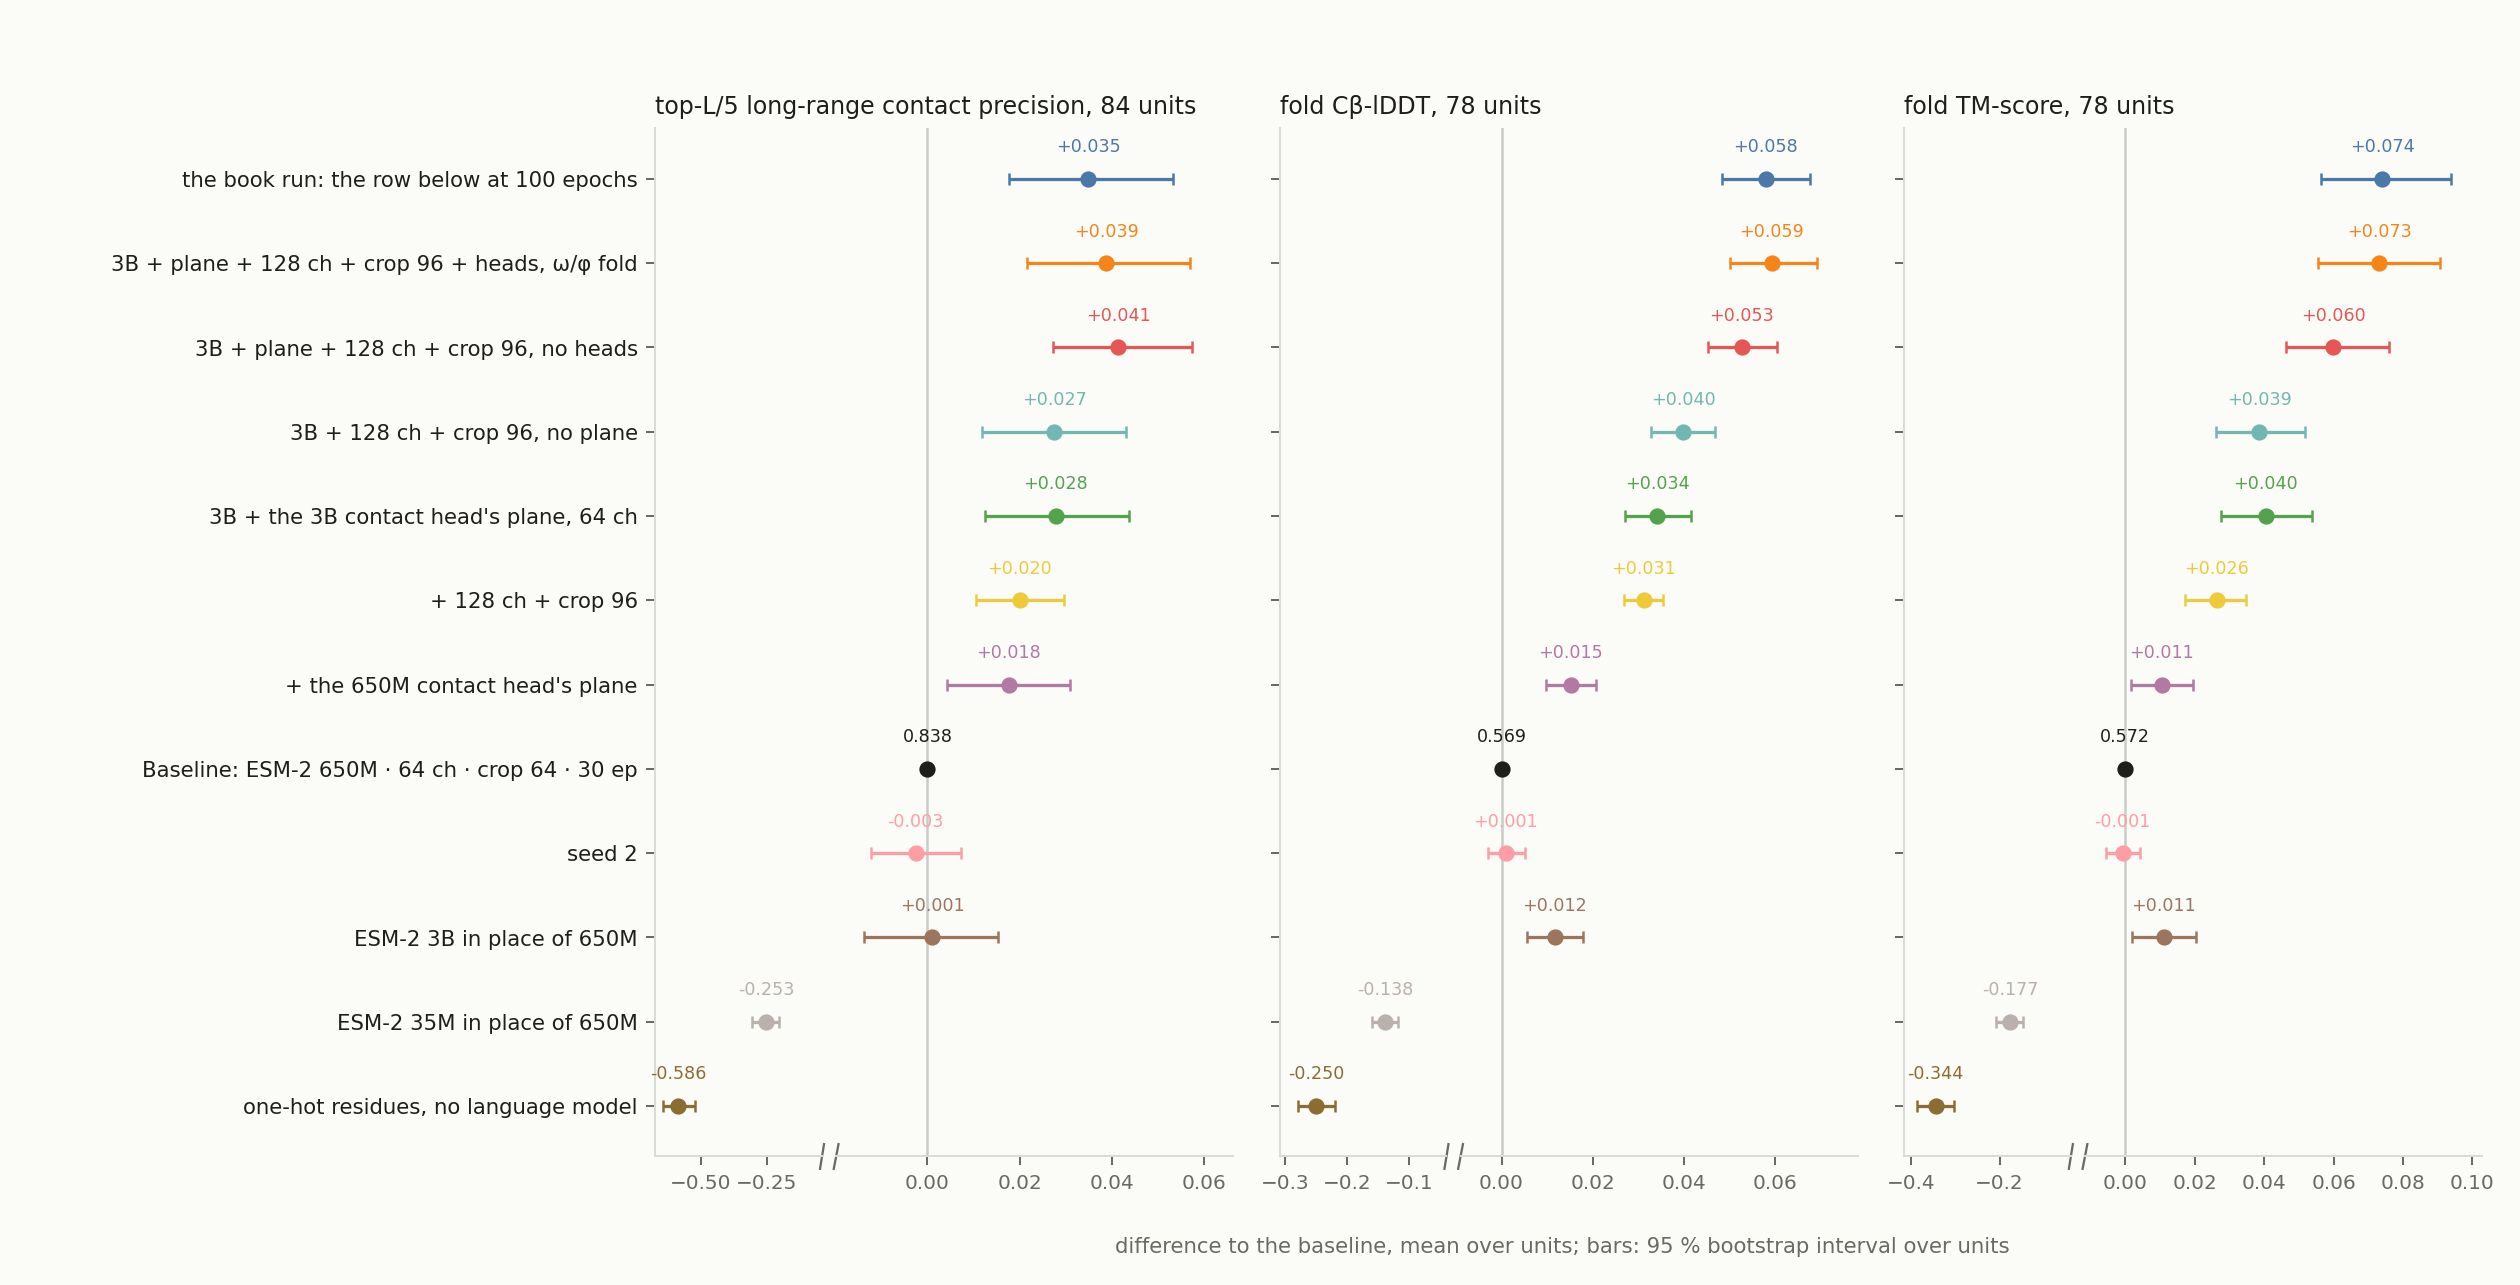
\includegraphics[width=\textwidth]{demos/casp16_ablation.png}
\caption{What each lever buys. Mean paired difference to the ESM-2 650M
baseline (64 channels, 64-residue crop, 30 epochs) over the evaluation
units, with a 95\,\% bootstrap interval over units: top-$L/5$ long-range
precision over the 84 units, the fold's $\mathrm{C}_\beta$-lDDT and TM-score over the 78.
The axis is broken where the language-model swaps sit. ``Plane'' is the
language model's own contact map as a pair channel, ``heads'' the
orientation heads with the $\omega/\varphi$-restrained fold; the rows
above the baseline stack those levers up to the book run.}
\label{fig:casp16_ablation}
\end{figure}

The gap is the story. Our TM-score of 0.646 sits at the field's third
percentile; the median first model is 0.892 over the same 78 units, $0.945
/ 0.883 / 0.656$ on the easy, medium and hard classes against our $0.716 /
0.617 / 0.495$, and OpenComplex, the lowest of the thirty groups that
predicted all 78, is at 0.768. Two readings, from the units themselves.
Sixteen units have top-$L/5$ precision under 0.85 and fold to 0.34 where
the field's median is 0.83 --- four of them ``easy'', which in CASP's
vocabulary means a template exists in the PDB, something a
single-sequence model cannot see --- and they are two fifths of the
distance; the other 62 fold to 0.72 against 0.91, and there the top $L/5$
pairs are right, the next $L$ are half wrong and the recall at $P > 0.5$ is
0.49. ESMFold places the two halves: the same language model under the
trunk and structure module its authors trained for it folds the 78 to
$0.751 / 0.778$, $+0.132$ of TM-score over our head with a 95\,\% interval
of $[+0.103, +0.167]$ and better on 71, 0.84 against 0.72 on the 62 units
where our top contacts are right and 0.53 against 0.34 on the 16 where
they are not. So the head is the larger half of the gap and the input is
the other: an alignment is what the field's models read and ESMFold does
not, and half of the sixteen are blind to the language model too.

What this is not: a 5.4M-parameter network on a single sequence, 65
residues of receptive field in a 96-residue window, folded as one point
per residue. The field's models read alignments and templates and build an
all-atom chain through a structure module; the architecture that does so
is the \bestiaryref{bestiary:evoformer}{Evoformer entry}, and AlphaFold~2's distogram head is this demo's
network grown into a 48-block pair stack with the alignment beside it.

Four gates sit under the table. The scorer reproduces CASP16's official
lDDT and TM-score to the printed digit on nine field models --- AF3-server,
MULTICOM and ColabFold on three targets --- and GDT\_TS within a point.
Folding a target's true distogram recovers its structure (TM-score 0.9999
on T1235-D1) and the mirror scores 0.34. The packed training pools are
checked against the per-chain files before any run, and a 64-chain
memorization probe must leave the separation prior. And \texttt{lake exe
distogram-casp smoke} finite-differences the emitted gradient of the pair
tile's weights, a body weight and each head's bias against the step's own
first Adam moment, and checks that the evaluation forward's loss at one
batch's statistics is the training step's. The trainer is
\texttt{demos/MainDistogramCasp.lean}; the chain list, labels, embeddings
and packing are \texttt{scripts/datasets/\allowbreak casp16\_*.py}, the
fold, scoring, table and figures \texttt{scripts/demos/\allowbreak
casp16\_*.py}.

\subsection*{AlphaFold 2 Evoformer (\texttt{Bestiary/Evoformer.lean})}
\phantomsection\label{bestiary:evoformer}
\emph{Two} new primitives (Definition~\ref{layer:evoformerBlock},
Definition~\ref{layer:structureModule}). Dual-representation (MSA + pair)
doesn't fit a linear \texttt{NetSpec} cleanly; the bestiary shows the
two bundled primitives and notes the limitation (Jumper et al.\ 2021,
\href{https://www.nature.com/articles/s41586-021-03819-2}{Nature}). Variants: full (76M), mini, tiny.


\begin{verbatim}
def alphaFold2 : NetSpec where
  name   := "AlphaFold 2 (Evoformer + StructureModule)"
  imageH := 384                                   -- max residues (N_res)
  imageW := 1
  layers := [
    -- 48 blocks of dual-representation processing (MSA + pair).
    -- Each block bundles: MSA row-attn (w/ pair bias), MSA col-attn,
    -- MSA transition, outer-product mean → pair, triangle-mul updates
    -- (out + in), triangle self-attention (start + end), pair transition.
    .evoformerBlock 256 128 48,
    -- Structure Module: 8 recurrent IPA rounds (weights shared).
    .structureModule 384 128 8
  ]
\end{verbatim}

The two primitives are conceptually separate networks chained back to
back; the linear \texttt{NetSpec} flattens that.

\textbf{Evoformer} (48 blocks) is the perception/refinement stage. It
maintains a dual representation: a multiple-sequence-alignment
tensor $\mathrm{MSA}\!\in\!\mathbb{R}^{s \times r \times c_m}$ (where
$s$ is the number of homologs found by the database search and $r$ is
the number of residues) and a pair tensor
$\mathrm{Pair}\!\in\!\mathbb{R}^{r \times r \times c_z}$ encoding
predicted residue-residue relationships. Each block updates both via
seven stacked operations (row attention with pair bias, column
attention, MSA transition, outer-product-mean into pair, two triangle
multiplicative updates, two triangle attentions, pair transition).
Forty-eight rounds of that turn raw evolutionary signal into a
self-consistent geometry-implied pair representation.

\textbf{Structure Module} (8 recurrent rounds, shared weights) is the
geometry stage. It consumes the final pair tensor + a per-residue
``single'' embedding and emits 3D backbone frames plus side-chain
$\chi$ angles. Each round runs Invariant Point Attention (IPA) over
the residues, updates each residue's local frame relative to its
neighbors, and feeds back into the next round. The shared-weights
recurrence is unusual --- most networks unroll different parameters
per layer --- and reflects that each round is the same fixed-point
iteration on the protein's 3D structure.

The bundled-primitive shortcut means Lean sees one \texttt{NetSpec}
with two layers; the actual graph is a much larger DAG with the dual
representation and the cross-stage handoff. Definition~\ref{layer:evoformerBlock}
and Definition~\ref{layer:structureModule} document the bundling explicitly.


\chapter{Game theory}
\label{chap:bestiary_games}

Three games written in Lean, each with its own exact instrument, on one loop: the
reward is the game's, the data is manufactured by playing it, the target is the model's
own later estimate, and the ceiling is exact where the game allows it --- poker's by
the best response to the trained strategy, tic-tac-toe's by the solved game --- and,
for Pong, a twin fed the six numbers the renderer draws from. The ladder runs a DQN
from pixels, then regret minimisation under hidden information, then self-play and
tree search, then search inside a learned model; every rung goes through the
squared-error block of the diffusion demo with a host-built target, and none of it
is new codegen but MuZero's unrolled model. The catalogue beside the
demos is the AlphaGo family and Deep CFR, the same loops at the scale that made them
famous.

\section{Pong --- DQN from pixels against the six-number state}
\label{sec:game_pong}

\texttt{demos/MainPongDqn.lean} is Mnih et al.'s DQN (2015,
\href{https://www.nature.com/articles/nature14236}{Nature}) on a Pong written in Lean
(\texttt{LeanMlir/Pong.lean}: an $84 \times 84$ field, two-pixel paddles, frame skip 4,
a scripted opponent that tracks the ball at 1.5 pixels a frame after a four-frame
delay, a game to 21, deterministic from a seed, five million raw frames a second with
no emulator and no ROM). Three things change relative to everything trained so far.
There is no dataset: transitions come from playing the game $\varepsilon$-greedily
against the current network, $\varepsilon$ from 1 to 0.1 over the first 100k agent
steps, into a replay of 100k transitions from which each gradient step samples 32, one
step per four agent steps, Adam at $10^{-4}$, 500k agent steps --- two million frames.
The target is the model's own prediction one step later,
$y_a = r + \gamma \max_{a'} Q_{\text{target}}(s', a')$ at $\gamma = 0.99$, with the
target network a copy of the online parameters refreshed every 1,000 updates. And the
loss is the squared-error block the DDPM demo trains with
(\S~\ref{sec:bestiary_diffusion}): the host runs the eval graph on the batch, writes
$y = Q(s,\cdot)$, overwrites the taken action's slot with the Bellman target and hands
$y$ in, so the gradient is zero on the untaken slots and a per-sample TD error on the
taken one. Zero new codegen. Two things are the pixels' own: the observation is an
image, so the Q-function is
Chapter~3's CNN kit at $84 \times 84$ (three convolutions with pooling standing in for
the paper's strides, a dense 512, three outputs; 1.7M parameters), and one frame does
not contain the ball's velocity, so the input is a stack of the last four. The bracket
is built into the game: the same DQN on the six numbers the renderer draws from ---
ball position and velocity, the two paddles, through a two-hidden-layer MLP of width
64, 4{,}803 parameters --- is a twin that is handed everything the pixels could carry,
the scripted opponent is the bar, and a one-frame input is the ablation.
Figure~\ref{fig:pong_dqn} is one input and the learning curves of those arms
(\texttt{runs/2026-09-25-pong-dqn/}).

\begin{figure}[H]
\centering
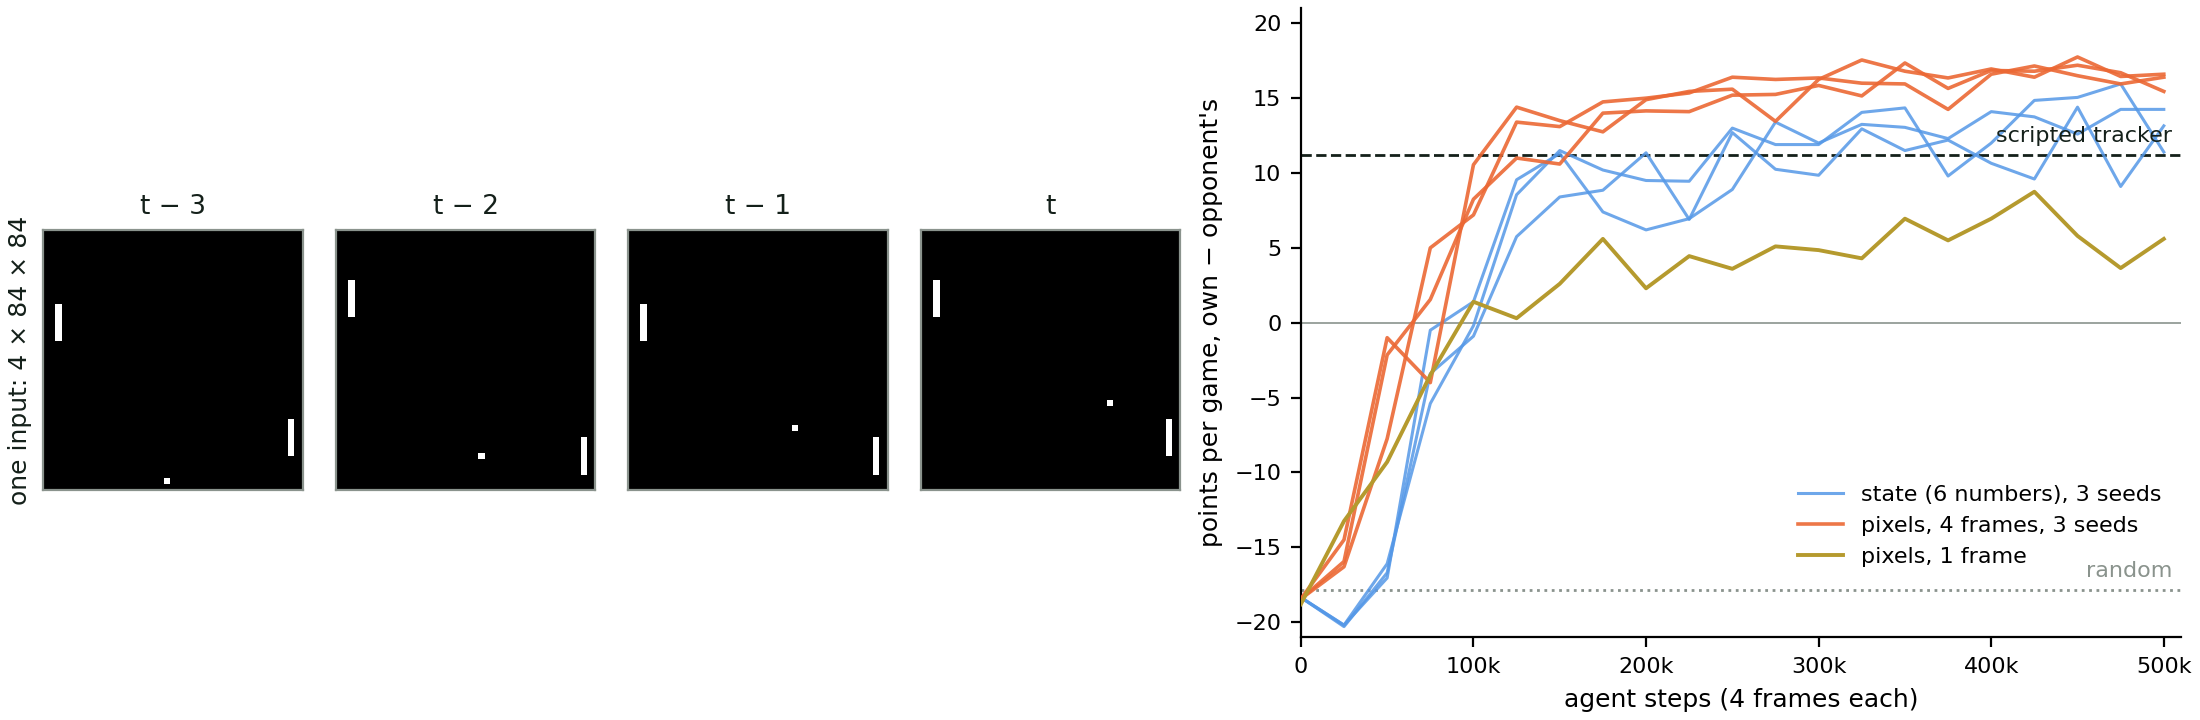
\includegraphics[width=\textwidth]{demos/pong_dqn.png}
\caption{Left: one input of the pixel network --- the four stacked $84 \times 84$
frames as the network saw them at an evaluation, the ball crossing toward the right
paddle. Right: points per game (own minus the opponent's, twenty games at
$\varepsilon = 0.05$) against agent steps, for the six-number state twin (three
seeds), the four-frame pixel network (three seeds) and the one-frame ablation, with
the random and scripted-tracker baselines as lines.}
\label{fig:pong_dqn}
\end{figure}

\paragraph{Every arm against the scripted opponent.} Table~\ref{tab:pong_arms} is the
mean points per game over twenty fresh games after training, with the standard
error; the baselines over a hundred games (\texttt{lake exe pong-env 100}). Each
arm is 500k agent steps on one card, five to seven minutes for a state run and
27 for a pixel run.

\begin{table}[H]
\centering
\caption{The Pong arms against the scripted opponent, in points per game (\texttt{runs/2026-09-25-pong-dqn/}; the stacked and the wide state arms, \texttt{runs/2026-10-27-pong-state-arms/}).}
\label{tab:pong_arms}
\begin{tabular}{@{}l l l@{}}
\hline
arm & points per game & first positive evaluation \\
\hline
random                           & $-17.88 \pm 0.20$ & --- \\
scripted tracker                 & $+11.18 \pm 0.37$ & --- \\
pixels, one frame                & $+4.60 \pm 1.48$ & 100k steps \\
state, six numbers, width 64, seeds 1--3   & $+14.15$, $+12.70$, $+13.50$ & 100--125k \\
\quad four states stacked, width 64, seeds 1--3 & $+13.45$, $+9.20$, $+10.55$ & 150--225k \\
\quad one state, width 512, seeds 1--3 & $+16.85$, $+12.75$, $+14.65$ & 75--100k \\
pixels, four frames, seeds 1--3  & $+15.60$, $+15.90$, $+14.90$ & 75--100k \\
\hline
\end{tabular}
\end{table}

\noindent One frame cannot see velocity, and the row says by how much: $+4.6$ against
$+15.5$, the gap between a paddle that reaches the ball and one that guesses. The
state twin was meant to be the ceiling and the 64-wide net is not: the pixel network
sits above it on every seed, $+15.47$ against $+13.45$ on average, and at every
opponent speed tried --- 1.0 / 1.5 / 2.0 pixels a frame, one seed each at 1.0 and
2.0: state $+14.45$ / $+13.45$ / $+9.80$, pixels $+17.75$ / $+15.60$ / $+14.45$,
where the 1.5 entries are the state net's three-seed mean and the pixel network's
seed 1. The six numbers are all the pixels could carry, so the gap was in the
networks, and the two other state rows say where. Stacking the last four states, as
the pixel network stacks frames, costs the state net 2.4 points ($+11.07$, the seed
spread tripled) and moves its first positive evaluation out to 150--225k steps: the
vector already carries the velocity the pixel network stacks frames to recover, and
the history is the same information four times over. Widening the one-state MLP to
the pixel network's dense width, 512, closes the gap: $+14.75$ against $+15.47$, a
difference smaller than the wide net's own seed spread, and level with the pixel
network at 200k steps where the 64-wide net was three to nine points behind. The
ordering was the 64-wide MLP's capacity, not the representation. An update on the
copying path was about 24 milliseconds with the GPU busy for four of them: the shim
re-pushed 20~MB of parameters and Adam moments every step. With that state resident
on the device (\texttt{trainStepAdamF32DdpmR}) the train step falls from 12.2 to
5.1 milliseconds and the loop, play and evaluations included, runs at 14.6
milliseconds an update; a pixel run is 27 minutes on one card.

\section{Poker --- Deep CFR against the exact best response}
\label{sec:game_leduc}

\texttt{demos/MainDeepCfrLeduc.lean} is Brown, Lerer, Gross and Sandholm's loop (Deep CFR,
ICML 2019, \href{https://arxiv.org/abs/1811.00164}{arXiv:1811.00164}) on Leduc hold'em
written in Lean (\texttt{LeanMlir/Leduc.lean}): a two-player, fixed-limit, one-card poker
--- $r$ ranks in two suits, three for the classic jack--queen--king deck, an ante of one,
two betting rounds with bets of two then four and at most two raises each, one public
card between the rounds, a pair beats a higher rank --- and the chapter's one game
with hidden information. The answer is therefore not a move but a mixed
strategy: an equilibrium raises a jack it knows is losing about a fifth of the time,
because a player who never bluffs can be read. Each iteration and player, one batched
forward of the player's advantage network over \emph{every} information set gives the
current strategy as a table (regret matching on the positive advantages), a thousand
external-sampling traversals in C write instantaneous regrets to the player's advantage
reservoir and the opponent's strategy to a strategy reservoir (reservoir sampling, a
million rows each), and the advantage network is re-initialised and retrained from
scratch on its reservoir, a thousand Adam steps at batch 512. After a hundred iterations
the strategy network is trained on the strategy reservoir; Single Deep CFR (Steinberger
2019, \href{https://arxiv.org/abs/1901.07621}{arXiv:1901.07621}) comes for free, the
exact average of the hundred stored profiles weighted by iteration and by each profile's
own reach, no strategy network. The network is the Leduc papers' three dense layers of
64 (\texttt{Bestiary/DeepCFR.lean}, 10.5k parameters, no BatchNorm), and the loss --- a
weighted squared error on the legal slots --- goes through the squared-error block as a
host-built target, tic-tac-toe's move. Two things change relative to Pong and the two
tic-tac-toe sections that follow:

\begin{itemize}
  \item \textbf{The instrument is the best response, and it is exact.} Suits never matter
    in Leduc (there are no flushes), so the game is solved at rank level --- $6r + 30r^2$
    information sets, 288 at $r = 3$ against OpenSpiel's 936 suit-aware ones, which fold
    onto them one-to-one --- by vector-form CFR over the public tree with an $r \times r$
    matrix of private ranks at each node: the best response, exploitability (the best
    responder's winnings per hand averaged over the two seats, OpenSpiel's convention),
    head-to-head and CFR+ to a thousand iterations are 25 milliseconds at $r = 3$ and
    under a second at $r = 13$. Zero is Nash; CFR+ reaches $2.4 \times 10^{-4}$. Before
    anything trains, the Lean game is checked against the C tree on every terminal
    history and both against OpenSpiel's \texttt{leduc\_poker}: every payoff on
    OpenSpiel's own histories, and our tables scored by OpenSpiel's exploitability to
    $10^{-6}$ (\texttt{scripts/demos/leduc\_gate0\_openspiel.py}).
  \item \textbf{The sampled table is the bracket, at the same budget.} A table is enough
    at every $r$ here, so the comparison is the Deep CFR paper's own axis: exploitability
    against nodes touched, external-sampling MCCFR on a table against the network, at
    $r = 3$, 6 and 13. The trainer's own traversal with a lookup table in the network's
    place must reproduce that curve before the network is trusted
    (\texttt{mode=tabular}), and does.
\end{itemize}

Figure~\ref{fig:deep_cfr_leduc} is one hand's betting tree under the trained
profile, the exploitability curves, and the bluff.

\begin{figure}[H]
\centering
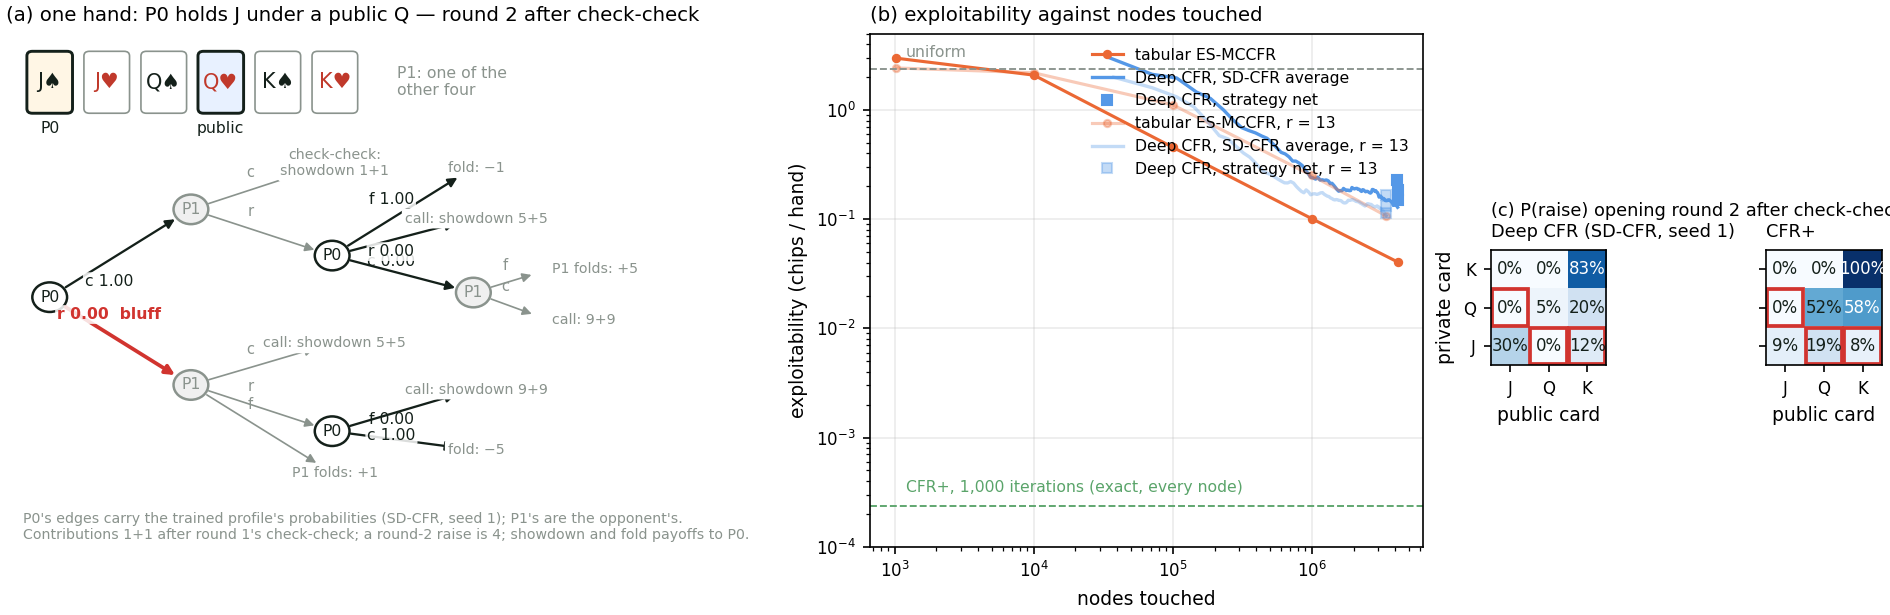
\includegraphics[width=\textwidth]{demos/deep_cfr_leduc.png}
\caption{Left: one hand --- the six cards, P0 holding a jack under a public queen ---
and round 2's betting tree after check-check from P0's seat, with the trained profile's
probability on each of P0's edges; the red edge is the bluff, raising the worst hand,
which this profile never takes. Middle: exploitability against nodes touched, log--log
--- tabular ES-MCCFR, Deep CFR as SD-CFR's average after every iteration (mean of three
seeds), the strategy network's final point, CFR+ and the uniform policy as lines; $r = 3$
solid, $r = 13$ faded. Right: raise probability at round 2's first decision after
check-check per private and public card, the trained profile beside CFR+, the worst-hand
cells ringed.}
\label{fig:deep_cfr_leduc}
\end{figure}

\paragraph{Every arm against the best response.} Exploitability in chips per hand (ante
one; a thousandth of a chip is a milli-ante per game, the Leduc papers' unit) and
head-to-head against CFR+ averaged over the two seats. The scripted honest arm raises a
pair or a king and folds a jack to a bet; the price-of-honesty arm is CFR+ with its
worst-hand raises moved to call; the two Deep CFR rows and the sampled table are at the
same 4.1M nodes, three seeds each, 5.7 minutes a seed on one card
(\texttt{runs/2026-10-08-deep-cfr-leduc/}). The last column of Table~\ref{tab:leduc_arms} is
the bluff, the raise frequency opening round 2 with a jack under a queen.

\begin{table}[H]
\centering
\caption{The Leduc poker arms at $r = 3$: exploitability, head-to-head against CFR+, and bluff frequency, per seed where three are given.}
\label{tab:leduc_arms}
\small
\begin{tabular}{@{}l l l l@{}}
\hline
arm & exploitability & vs CFR+ & bluff \\
\hline
uniform random              & 2.374 & $-0.707$ & 50\% \\
scripted honest             & 1.050 & $-0.123$ & 0\% \\
CFR+, bluffs moved to call  & 0.186 & $-0.012$ & 0\% \\
Deep CFR, strategy network  & 0.229 / 0.185 / 0.152 & $-0.055$ / $-0.039$ / $-0.050$ & 1.6\% / 0.8\% / 6.4\% \\
Deep CFR, SD-CFR average    & $\mathbf{0.127}$ / $\mathbf{0.150}$ / $\mathbf{0.109}$ & $-0.022$ / $-0.031$ / $-0.020$ & 0.0\% / 5.5\% / 6.3\% \\
tabular ES-MCCFR            & 0.038 / 0.043 / 0.041 & $-0.007$ / $-0.010$ / $-0.009$ & 9.5\% / 11.7\% / 2.2\% \\
CFR+, a thousand iterations & 0.00024 & 0 & 19.5\% \\
\hline
\end{tabular}
\end{table}

\noindent Deep CFR's exploitability falls from 1.4 at
iteration 5 to 0.11--0.15 at a hundred and ends under the honest arm and under the
equilibrium with its bluffs removed; at a hundred iterations it is where the Single
Deep CFR paper's Leduc curves are (150--200 milli-antes per game read from its Figure
1a, at 1,500 traversals an iteration to our thousand). It does not beat a sampled table
at the same budget on the classic deck: the table is three times less exploitable at
4.1M nodes. The scale arm is where that turns. The same recipe at $r = 6$ (1,116 sets)
and $r = 13$ (5,148): SD-CFR 0.112 / 0.123 / 0.113 against the table's 0.053 / 0.066 /
0.058 at 3.6M nodes, then 0.099 / 0.120 / 0.106 against 0.113 / 0.107 / 0.102 at 3.4M ---
the table's lead is $3.1\times$, $2.0\times$, $1.0\times$, and at $r = 13$ the network is
the better head-to-head ($-0.028$ against $-0.035$ a hand). The table visits all but a
set or two at these budgets, so the mechanism is not what it never saw; its estimate of each set
is noisier as the sets multiply at a fixed budget, and the network's error does not grow
with them. The bluff column is the finding a reader can check on
Figure~\ref{fig:deep_cfr_leduc}: the
trained profile that is 0.13 exploitable raises the losing jack under a queen 0.0\% of
the time, and the other two seeds 5.5\% and 6.3\%, where the equilibrium raises it
19.5\% (18.6--19.5\% over two solvers and three initialisations --- the frequency is
pinned at $r = 3$, and is not at $r = 13$, where the same cell ranges over tens of
points), and it bluffs elsewhere instead, a jack under a king 11--17\% across the three
seeds. Honesty's price is exact: moving the equilibrium's worst-hand raises
to call costs 0.186 of exploitability.

What this is not: a two-player, fixed-limit, one-card game, solved at rank level. The
scale of the Deep CFR paper is heads-up flop and limit hold'em, where no exact best
response exists to score against and the paper's numbers are against abstractions and
head-to-head; no-limit and multi-way poker (Pluribus) are another scale again, and
exploitability is not computable there.

\section{Tic-tac-toe --- AlphaZero against the solved game}
\label{sec:game_ttt}

The \texttt{demos/MainAlphaZeroTtt.lean}
trainer is Silver et al.'s self-play loop (AlphaGo Zero, 2017,
\href{https://www.nature.com/articles/nature24270}{Nature}; AlphaZero, 2018,
\href{https://www.science.org/doi/10.1126/science.aar6404}{Science}) on tic-tac-toe
written in Lean (\texttt{LeanMlir/TicTacToe.lean}), $n \times n$ with $k$ in a row,
$n$ the one knob. Each iteration plays 256 games in lockstep: at every move a PUCT
search of 25 ($3 \times 3$) or 100 ($4 \times 4$) simulations over the network's
priors and value, one batched forward over the games' pending leaves per simulation,
Dirichlet noise at the root, the move drawn from the visit counts; the visit
distribution $\pi$ and the outcome $z$ are the targets, and the next iteration plays
with the new network. The network is AlphaGo's plain convolution + ReLU stack
(\texttt{Bestiary/AlphaGo.lean}) at tic-tac-toe width, with the policy and value
heads merged into one dense output of $n^2 + 1$ slots: 78k parameters at
$3 \times 3$, 155k at $4 \times 4$. Three things change relative to Pong's DQN:

\begin{itemize}
  \item \textbf{The loss has two heads and the codegen has one.} The paper's
    $(z - v)^2 - \pi^{\top} \log p$ goes through the squared-error block Pong's
    Bellman target went through: the host runs the eval graph on the batch and writes
    $y = \mathrm{out} - \tfrac{n_{\mathrm{out}}}{2}\, g$, with
    $g = \mathrm{softmax}(p) - \pi$ on the $n^2$ policy slots and
    $(\tanh v - z)(1 - \tanh^2 v)$ on the value slot, so the block's gradient is
    $g / B$ exactly --- the gradient of the batch-mean AlphaZero loss. Zero new
    codegen, the move the neural-quantum-state demo (\S~\ref{sec:bestiary_beyond})
    makes with its energy gradient.
  \item \textbf{Not the bestiary's tower.}
    \texttt{Bestiary/AlphaZero.lean}'s convolution--BatchNorm--residual body is
    the wrong instrument here. BatchNorm's batch statistics over nine binary cells
    are a liability, and with BatchNorm the eval forward the loss reads and the
    train step's forward are different functions. Pong made the same
    choice for the same reason.
  \item \textbf{The instrument is the solved game.} A position is a base-3 number
    over the cells, so a memoised minimax fills one byte per index with the exact
    value and the optimal-move set of every reachable position --- 5,478 at
    $3 \times 3$, 9,722,011 at $4 \times 4$. The network alone is scored by the
    argmax of its masked logits over \emph{every} reachable decision position (4,520
    and 9,062,619), its value head against the exact value, and its match play
    against a perfect player that draws uniformly from the optimal set. Nothing in
    the table is sampled but the games.
\end{itemize}

\paragraph{Five by five, four in a row.} No table exists there ($3^{25}$ bytes), so the
instrument becomes an exact solver --- alpha-beta with a transposition table over
symmetry-canonical positions --- checked against the dense table on every reachable
$3 \times 3$ and $4 \times 4$ position before it is trusted where no table exists. It
establishes that $(5, 5, 4)$ is a draw, and something a reader can check on
Figure~\ref{fig:alphazero_ttt}: after X takes the centre, O's only drawing replies are the four diagonal
neighbours. Two things change in what the table can say: the sweep is a fixed sample
of 20,000 random-play decision positions with at least six stones, exact per position
but not exhaustive; and the perfect player draws its first move uniformly from the
optimal set and plays the solver's principal move from there.

\begin{figure}[H]
\centering
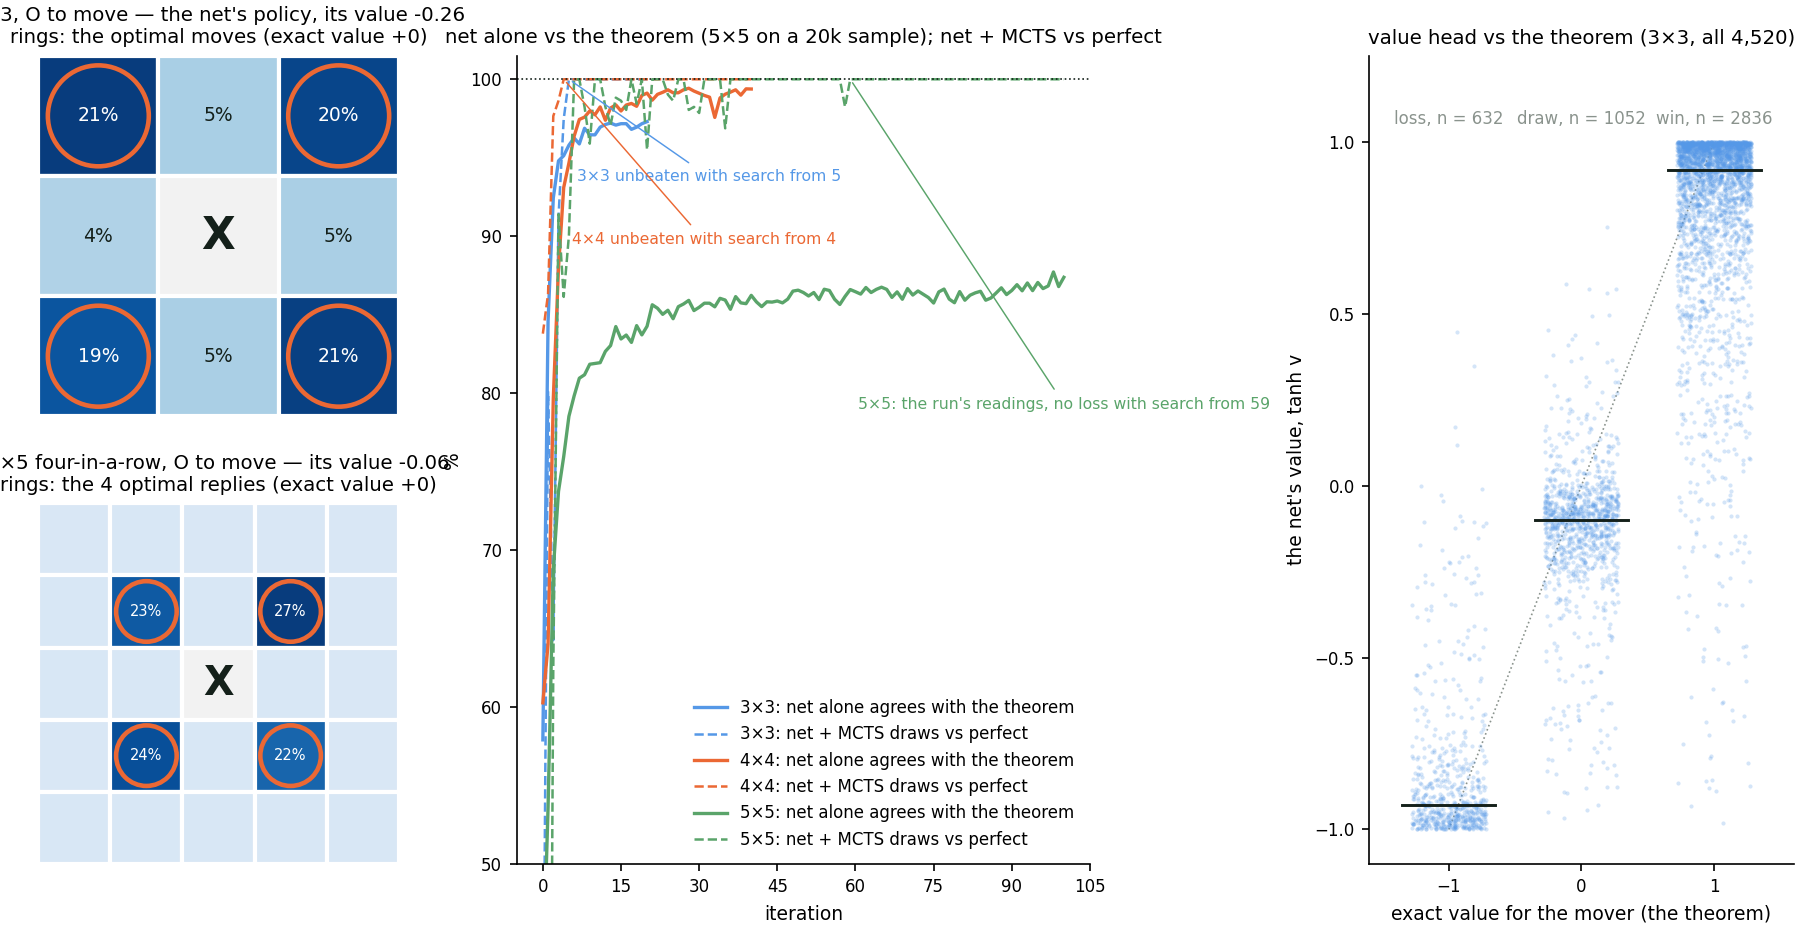
\includegraphics[width=\textwidth]{demos/alphazero_ttt.png}
\caption{Left, above: X in the centre, O to move --- the trained $3 \times 3$
network's move probabilities over the empty cells, with the solved game's optimal moves
ringed: the corners draw, the edges lose, and the network puts 81\% on the corners.
Left, below: the same position at $5 \times 5$, four in a row, where the solver says
O's only drawing replies are the four diagonal neighbours, and the trained network puts
24\% on each. Middle: agreement of the network alone with the solved game --- over
every reachable decision position at $3 \times 3$ and $4 \times 4$, over a 20,000-position
sample at $5 \times 5$ --- against iteration, with the draw rate of network + search
against the perfect player dashed; unbeaten with search from iteration 5 and 4. Right: the value head against the exact value of all 4,520 $3 \times 3$
decision positions, one dot per position, medians as bars.}
\label{fig:alphazero_ttt}
\end{figure}

\paragraph{Every arm against the solved game.} Table~\ref{tab:ttt_arms} is the agreement
of the arm's move with the optimal set --- over every decision position at $3 \times 3$ and $4 \times 4$, over the
20,000-position sample at $5 \times 5$; the scripted players' is their expected
agreement --- and W/D/L against the perfect player as X and as O: 1,000 games each way
for the scripted rows (200 at $5 \times 5$), and for the network's rows three
independent evaluations of the saved network, 256 games each, pooled.

\begin{table}[H]
\centering
\caption{The tic-tac-toe arms against the solved game at $3 \times 3$, $4 \times 4$ and $5 \times 5$: twenty iterations at $3 \times 3$, forty at $4 \times 4$ and a hundred at $5 \times 5$, the same binary with \texttt{n=4} and \texttt{n=5 k=4}.}
\label{tab:ttt_arms}
\small
\begin{tabular}{@{}l r l r l r l@{}}
\hline
 & \multicolumn{2}{c}{$3 \times 3$} & \multicolumn{2}{c}{$4 \times 4$} & \multicolumn{2}{c}{$5 \times 5$, four in a row} \\
arm & agrees & vs perfect, X $\cdot$ O & agrees & vs perfect, X $\cdot$ O & agrees & vs perfect, X $\cdot$ O \\
\hline
random           & 58.0\% & 0/207/793 $\cdot$ 0/33/967   & 60.4\% & 0/487/513 $\cdot$ 0/341/659 & 45.0\% & 0/0/200 $\cdot$ 0/0/200 \\
win-or-block     & 94.0\% & 0/831/169 $\cdot$ 0/215/785  & 95.6\% & 0/930/70 $\cdot$ 0/840/160  & 77.0\% & 0/7/193 $\cdot$ 0/1/199 \\
network alone    & $\mathbf{97.3\%}$ & 0/768/0 $\cdot$ 0/768/0 & $\mathbf{99.4\%}$ & 0/768/0 $\cdot$ 0/768/0 & $\mathbf{87.4\%}$ & 0/768/0 $\cdot$ 0/708/60 \\
network + search & ---    & 0/768/0 $\cdot$ 0/768/0      & ---    & 0/768/0 $\cdot$ 0/768/0      & ---    & 0/768/0 $\cdot$ 0/745/23 \\
perfect          & 100\%  & 0/1000/0 $\cdot$ 0/1000/0    & 100\%  & 0/1000/0 $\cdot$ 0/1000/0    & 100\%  & 0/200/0 $\cdot$ 0/200/0 \\
\hline
\end{tabular}
\end{table}

\noindent The $3 \times 3$ run is 2.5 minutes on one card and the $4 \times 4$ run 10.0
minutes (\texttt{runs/2026-09-29-alphazero-ttt/}); the estimate for the Python
implementation this loop follows (Nair,
\href{https://github.com/suragnair/alpha-zero-general}{alpha-zero-general}) on the
$4 \times 4$ board was 20--24 hours. The untrained network's sweep is the random player's. Self-play visits 1.2\%
of the $4 \times 4$ decision positions and the sweep scores all of them; the misses
are mostly forced wins not taken, late in games a competent opponent never produces,
and the search closes them --- with 25 or 100 simulations the network is unbeaten
from iteration 5 and 4, before the network alone is. The value head estimates
self-play rather than the theorem (the right panel of Figure~\ref{fig:alphazero_ttt}): the root ends
X-favoured at $3 \times 3$ because self-play under root noise is. At $5 \times 5$
the same binary with \texttt{n=5 k=4} runs a hundred iterations at 400 simulations
in 64 minutes. As X the network never loses, alone or with search; as O it still
does --- 60 games in 768 alone, 23 with search --- and its 87.4\% on the random-play
sample is 92.1\% over the exhaustive opening, every position with at most three
stones: it is best where the theory is. On this board the search is what closes the
second player's games, and at a hundred iterations it has not closed them.

\section{Tic-tac-toe without the rules --- MuZero against the solved game}
\label{sec:game_muzero_ttt}

The \texttt{demos/MainMuZeroTtt.lean} trainer is Schrittwieser et al.'s MuZero
(2020, \href{https://www.nature.com/articles/s41586-020-03051-4}{Nature}) on the
same instrument. AlphaZero is handed the rules: its search calls \texttt{step}.
MuZero is not. Three plain convolution stacks --- a representation $h$ from the two
stone planes to a $32 \times n \times n$ latent, a dynamics $g$ from a latent and a
one-hot move plane to the next latent, and AlphaZero's two-headed prediction $f$ ---
plus a one-output reward network $r$ on the latent a move reaches, 137k parameters at
$3 \times 3$ and 141k at $4 \times 4$, are trained end to end on $K = 5$ moves of
stored games: the policy, value and reward targets at every unrolled step, the
latent min--max normalised after every network as in the paper. The search is PUCT in
the latent: a node is a path, one batched $g$ over every game's pending leaf per
simulation, then one $f$ and one $r$; legal moves are masked at the root from the real
rules and nowhere inside the tree. Win rate cannot tell this agent from AlphaZero ---
both are unbeaten --- so the question the section asks is the one the solved game can
answer exactly: \emph{did MuZero learn tic-tac-toe, or only its values?} The
literature predicts the second (Grimm et al.\ 2020's value-equivalence principle,
\href{https://arxiv.org/abs/2011.03506}{arXiv:2011.03506}; He, Moerland, de Vries and
Oliehoek 2023, \href{https://arxiv.org/abs/2306.00840}{arXiv:2306.00840}, find MuZero's
model accurate on the policy it trained with and poor on others, measured against
estimated returns). Here the
answer is exact at every position, after every number of imagined moves, on lines
the agent plays and lines it never would. Three things change relative to AlphaZero:

\begin{itemize}
  \item \textbf{One new codegen piece.} The kit emits a train step --- forward,
    backward and optimizer in one call --- and an eval forward. MuZero's loss reaches
    $h$ and $g$ through the unroll $s_0 = h(o)$, $s_{k+1} = g(s_k, a_k)$, so $g$'s
    backward has to hand a cotangent to the previous step and $h$'s receives the sum of
    everything downstream. \texttt{MlirCodegen.generateVjp} is the existing backward
    walk with the first layer's input gradient --- every convolution already emits one
    through \texttt{conv2dHasVJP3}, returned rather than dropped, with no
    optimizer tail; \texttt{generateApplyAdam} is the existing Adam update on its own.
    The trainer composes the gradient by hand, in reverse over the unroll, with the
    min--max's VJP and the paper's two scalings on the host. Gated before any game code:
    $\theta - \partial\theta$ from the VJP module equals the SGD train step's $\theta'$
    bit for bit on all 136,787 parameters of the four $3 \times 3$ networks; the
    input cotangent agrees with central differences and with \texttt{jax.vjp}; the
    four composed gradients of the unrolled loss agree with \texttt{jax.grad} of the
    same loss written as one JAX function to $7 \times 10^{-7}$ on the CPU compiler
    (on XLA's CUDA path, $2$--$7 \times 10^{-4}$: TF32 convolutions, the level every
    XLA-against-reference tie in this book sits at).
  \item \textbf{A tree with no transpositions, gated against the one with them.}
    AlphaZero's search keys nodes by the true position's index, so two move orders
    reaching one board share a node. A latent tree cannot: a node is a path. The gate
    that catches search bugs replaces $g$ with the true dynamics --- the latent of the
    real next position --- and $f \circ h$ with a trained AlphaZero network cut after
    its trunk, so both searches read the same two graphs: the position-keyed search's
    first transposition needs seven simulations, so at $2$ to $6$ simulations every
    root visit distribution must agree exactly, and all 4,520 do; a planted bug that
    drops the edge reward passes at 2 and fails at 3--6 on 898--2,168 positions.
  \item \textbf{The instrument scores the model, not only the player.} From every
    reachable decision position (a fixed every-454th sample of the 9,062,619 at
    $4 \times 4$), a legal line of $k = 0 \ldots 2K$ moves from three sources --- the
    agent's own policy, perfect play, uniform random legal moves --- is played
    \emph{inside the model}, and $f(g^k(h(s)))$ is scored against the exact value and
    optimal set of the true position the line reaches; $r$ against the true outcome of
    every move; and a closed-form ridge probe from the latent to the sixteen cell
    states, fit on $h$ of real positions and refit on $g$'s own latents at each depth,
    says whether the board is still linearly decodable --- the nearest thing to
    ``knows the board''. Every number is exact per position; at $3 \times 3$ every set
    is exhaustive.
\end{itemize}

Figure~\ref{fig:muzero_ttt} is one line played inside the model against the true
board, and the instrument's curves against imagined depth.

\begin{figure}[H]
\centering
\includegraphics[width=\textwidth]{demos/muzero_ttt.png}
\caption{Left: one $4 \times 4$ line played only inside the trained model, from a
real position (O to move) along five uniformly random legal moves. Top row the true
board; middle the board probe's readout of the imagined latent, cells the model has
lost in red; bottom $f$'s policy over the cells with the solved game's optimal moves
ringed. The model keeps every cell through four imagined moves and loses three at the
fifth, where it reads $-0.12$ for a position whose exact value is $-1$. Middle: policy
agreement with the optimal set (solid) and the value's sign (dashed) of $f(g^k(h(s)))$
against imagined depth $k$, from a 19,961-position sample of the $4 \times 4$ decision
positions, on the agent's own lines, perfect play and random lines, AlphaZero's
exhaustive root agreement dash-dotted, $K = 5$ dotted. Right: $r$'s recall of the
winning moves and the refit probe's whole-board accuracy against $k$, own and random
lines.}
\label{fig:muzero_ttt}
\end{figure}

\paragraph{Every arm against the solved game.} Table~\ref{tab:muzero_ttt_arms} adds
MuZero's rows to Table~\ref{tab:ttt_arms}'s protocol --- agreement over every decision
position, three independent 256-game evaluations of the saved network pooled against
the perfect player --- and two columns only a model can have: the policy's agreement
after $K = 5$ imagined moves on the agent's own lines and on random lines, and the
share of winning moves $r$ calls, over every legal move from every scored start. The
networks are the recipe that passed at $3 \times 3$ --- 50-simulation self-play, 300
Adam steps an iteration, the raw mean $Q$ --- on fresh initialisations, 60 iterations
at $3 \times 3$ and 120 at $4 \times 4$, ten minutes on one card and 26--27 minutes
(\texttt{runs/2026-10-20-muzero-ttt-4x4/}); at $4 \times 4$ all three initialisations
end the run unbeaten both sides, alone and with 25 and 100 simulations, and the table's
is the one with the highest root agreement.

\begin{table}[H]
\centering
\caption{The tic-tac-toe arms against the solved game, with MuZero's: 60 iterations at
$3 \times 3$ and 120 at $4 \times 4$, the same binary with \texttt{n=4}; the 600-step rows
double the Adam steps an iteration. ``Imagined'' is policy agreement after five moves inside
the model on the agent's own lines $\cdot$ random lines; ``$r$'' the winning moves the
reward network calls at one move.}
\label{tab:muzero_ttt_arms}
\small
\begin{tabular}{@{}l r l r l@{}}
\hline
arm & agrees & imagined, own $\cdot$ random & $r$ & vs perfect, X $\cdot$ O \\
\hline
\multicolumn{5}{l}{$3 \times 3$} \\
random                 & 58.0\% & --- & --- & 0/207/793 $\cdot$ 0/33/967 \\
win-or-block           & 94.0\% & --- & --- & 0/831/169 $\cdot$ 0/215/785 \\
AlphaZero alone        & $\mathbf{97.3\%}$ & --- & --- & 0/768/0 $\cdot$ 0/768/0 \\
AlphaZero + search     & ---    & --- & --- & 0/768/0 $\cdot$ 0/768/0 \\
MuZero alone           & 96.9\% & 100\% $\cdot$ 96.5\% & 93.0\% & 0/768/0 $\cdot$ 0/768/0 \\
MuZero + latent search & ---    & --- & --- & 0/768/0 $\cdot$ 0/768/0 \\
perfect                & 100\%  & --- & --- & 0/1000/0 $\cdot$ 0/1000/0 \\
\hline
\multicolumn{5}{l}{$4 \times 4$} \\
random                 & 60.4\% & --- & --- & 0/487/513 $\cdot$ 0/341/659 \\
win-or-block           & 95.6\% & --- & --- & 0/930/70 $\cdot$ 0/840/160 \\
AlphaZero alone        & $\mathbf{99.4\%}$ & --- & --- & 0/768/0 $\cdot$ 0/768/0 \\
AlphaZero + search     & ---    & --- & --- & 0/768/0 $\cdot$ 0/768/0 \\
MuZero alone           & 98.7\% & 100\% $\cdot$ 92.9\% & 99.5\% & 0/768/0 $\cdot$ 0/768/0 \\
MuZero + latent search & ---    & --- & --- & 0/768/0 $\cdot$ 0/768/0 \\
MuZero alone, 600 steps & 99.1\% & 100\% $\cdot$ 93.4\% & 100.0\% & 0/768/0 $\cdot$ 0/767/1 \\
MuZero + latent search, 600 steps & --- & --- & --- & 0/768/0 $\cdot$ 0/768/0 \\
perfect                & 100\%  & --- & --- & 0/1000/0 $\cdot$ 0/1000/0 \\
\hline
\end{tabular}
\end{table}

\noindent MuZero bootstraps slowly: AlphaZero's $4 \times 4$ network passes 93\% root
agreement by iteration 4, MuZero's sits at 62--66\% through iteration 40, 73\% at 50,
92\% at 60 and 98\% by 100 --- self-play stays decisive for a long time, so $z$ teaches
the values of weak play. A $4 \times 4$ run stopped at sixty iterations stands at 92.1\%
root agreement and still loses as O with search, six games in 256 at the run's own
evaluation; the 120-iteration runs are the table. Doubling the steps an iteration
brings the take-off to iteration 40 and the sweep to 99.1\%, the table's 600-step rows,
and costs one game in 768 alone as O. Self-play stood at 2.6\% of the decision positions.

\paragraph{What the model learned.} The value-equivalent prediction --- values, not the
board --- does not hold at one move and holds with depth. On the agent's own lines the
probe refit on $g$'s latents recovers 99.8\% of whole $4 \times 4$ boards after one
imagined move and 99.7\% after five; on random lines 94\% after one and 55\% after
five, and a line of random moves is where Figure~\ref{fig:muzero_ttt}'s model loses the
board. The
reward network calls 99.5\% of the winning moves at one move and 1.3\% of the others;
along random lines its recall falls to 45\% by the fifth. The value's sign holds on
the agent's own lines (92\% at the root, 99.8\% after five imagined moves, the surviving
lines being endgames) and falls to 79--80\% on random lines by the fourth --- He et
al.'s gap, against an exact value. Two move orders reaching one board land 2.0 apart in
the latent, against 4.5 from $h$ of that board and 5.2 between different boards: the
model keeps the board in its own encoding, not $h$'s. The probe fit on $h$ reads every
held-out real position and 96--97\% of the cells of $g$'s latents --- at $3 \times 3$
only 84\%, and the weaker the network, the less of the board $g$ keeps. What the
search does with the model's mistakes is the last line: at $3 \times 3$ a third to a
half of the positions where the search errs and the network alone does not carry a
phantom win on the principal line --- $r$ calling a win the true board does not have
--- against 1--2\% of other positions, and at the training budget extra simulations
cost O games on two of three initialisations; at $4 \times 4$ the search errs where
the network alone does not at 3 starts in 19,961, one of them with a phantom win, and
holds at 100 simulations on every initialisation.

\section{The catalogue: the AlphaGo family and Deep CFR}

The entries in this section are these loops at the scale that made them famous: the network is
a residual tower, the game is Go or chess, and the target is still the model's own
later estimate.

\subsection*{Deep CFR (\texttt{Bestiary/DeepCFR.lean})}
\emph{Zero} new primitives. Counterfactual regret minimisation with the two tables
replaced by networks (Brown, Lerer, Gross and Sandholm 2019): an advantage network per
player regresses the sampled counterfactual regrets of an information set and regret
matching on its positive outputs is the current strategy; an average-strategy network
regresses the strategies played, or, in Single Deep CFR (Steinberger 2019), the stored
advantage networks are averaged exactly instead. The paper's network is two branches ---
summed card embeddings through three dense layers, bet flags and sizes through two ---
concatenated into three more with skips where the widths agree and a normalisation of
the last layer's features, 98,948 parameters for heads-up flop hold'em; its Leduc
experiments and ours use three dense layers of 64. The architecture is not the point and
the paper says so; the loop is, and \S~\ref{sec:game_leduc} trains it.

\begin{verbatim}
def deepCfrLeducNet (r : Nat := 3) : NetSpec where
  name   := s!"Deep CFR Leduc r{r}"
  imageH := 1
  imageW := 1
  layers := [
    -- 2r + 24 features: one-hot cards with rank scalars, pair and
    -- above-public flags, the betting history, the round, the pot.
    .dense (2 * r + 24) 64 .relu,
    .dense 64 64 .relu,
    .dense 64 64 .relu,
    .dense 64 3 .identity          -- fold, call, raise
  ]
\end{verbatim}

\subsection*{AlphaGo (\texttt{Bestiary/AlphaGo.lean})}
\emph{Zero} new primitives. The original 2016 Lee Sedol system
(Silver et al.\ 2016,
\href{https://www.nature.com/articles/nature16961}{Nature}).
Three separate networks: a 13-layer conv \emph{policy} network
($\sim$3.9M) trained first on 30M human games then fine-tuned via
self-play, a 13-layer conv + FC-head \emph{value} network
($\sim$4M), and a shallow linear \emph{rollout} policy used inside
MCTS for fast tree playouts. Input is 48 hand-crafted Go feature
planes (liberties, ladder patterns, 3$\times$3 stone arrangements,
etc.). AlphaGo Zero (\bestiaryref{bestiary:alphagozero}{the AlphaZero entry}) throws all of this out --- raw
board only, one two-headed net, self-play only --- and plays better
(5185 Elo vs 3140). The one-sentence lesson is written into every
follow-up paper: features the network can learn on its own, it will.

\begin{verbatim}
def alphaGoPolicyNet : NetSpec where
  name   := "AlphaGo policy network"
  imageH := 19
  imageW := 19
  layers := [
    -- 13 conv layers: one 5×5 stem + eleven 3×3 at 192 channels.
    -- Plain conv+ReLU, no BatchNorm: 2016 AlphaGo predates both BN and
    -- residual blocks in this lineage (AlphaGo Zero added them).
    .conv2d 48 192 5 .same .relu,                 -- 48 hand-crafted planes in
    .conv2d 192 192 3 .same .relu, .conv2d 192 192 3 .same .relu,
    .conv2d 192 192 3 .same .relu, .conv2d 192 192 3 .same .relu,
    .conv2d 192 192 3 .same .relu, .conv2d 192 192 3 .same .relu,
    .conv2d 192 192 3 .same .relu, .conv2d 192 192 3 .same .relu,
    .conv2d 192 192 3 .same .relu, .conv2d 192 192 3 .same .relu,
    .conv2d 192 192 3 .same .relu,
    -- 1×1 conv to per-position move logit (reshape + pass scalar downstream)
    .conv2d 192 1 1 .same .identity
  ]
\end{verbatim}

\subsection*{AlphaZero (\texttt{Bestiary/AlphaZero.lean})}
\phantomsection\label{bestiary:alphagozero}
\emph{Zero} new primitives --- \texttt{convBn} + \texttt{residualBlock}
+ \texttt{dense}. Two-headed (policy + value) network
(Silver et al.\ 2018,
\href{https://arxiv.org/abs/1712.01815}{arXiv:1712.01815}),
expressed as two separate \texttt{NetSpec} values sharing the body in
prose. Variants: AlphaGo Zero (Go; Silver et al.\ 2017,
\href{https://www.nature.com/articles/nature24270}{Nature}),
AlphaZero chess, tiny fixture.

\begin{verbatim}
def alphaGoZeroPolicy : NetSpec where
  name   := "AlphaGo Zero (policy head)"
  imageH := 19
  imageW := 19
  layers := [
    .convBn 17 256 3 1 .same,                     -- 17 raw-history planes → 256
    .residualBlock 256 256 19 1,                  -- 19 residual blocks (shared body)
    .convBn 256 2 1 1 .same,                      -- policy head: conv→BN→ReLU, 2 ch
    .flatten,
    .dense (2 * 19 * 19) 362 .identity            -- 361 board moves + pass
  ]
\end{verbatim}

The value head shares the first two layers (body) and diverges at
the head --- one filter, two-layer MLP down to a single scalar
(\texttt{tanh} is applied downstream; \texttt{Activation} doesn't
include it):

\begin{verbatim}
def alphaGoZeroValue : NetSpec where
  name   := "AlphaGo Zero (value head)"
  imageH := 19
  imageW := 19
  layers := [
    .convBn 17 256 3 1 .same,                     -- shared body
    .residualBlock 256 256 19 1,                  -- shared body
    .convBn 256 1 1 1 .same,                      -- value head: conv→BN→ReLU (1 filter)
    .flatten,
    .dense (1 * 19 * 19) 256 .relu,
    .dense 256 1 .identity                        -- → scalar (tanh applied downstream)
  ]
\end{verbatim}

The chess variant keeps the 19-block tower on 119 input planes over an
\(8 \times 8\) board, and its policy head is convolutional as in Silver et
al.\ 2018: a convolution to 73 move planes, flattened into the 4672
logits, with no dense layer. The tiny fixture is 17 planes, 3 blocks, a
\(9 \times 9\) board.

\subsection*{MuZero (\texttt{Bestiary/MuZero.lean})}
\emph{Zero} new primitives --- three ResNet-style networks (representation,
dynamics, prediction) reusing \texttt{convBn} + \texttt{residualBlock}
+ \texttt{dense}. The architectural novelty is the three-network
factoring, not any single layer type (Schrittwieser et al.\ 2020,
\href{https://arxiv.org/abs/1911.08265}{arXiv:1911.08265}). Five \texttt{NetSpec} values per
variant (rep, dyn body, dyn reward head, pred policy, pred value).
Variants: Go, Atari (representation only), tiny.

\begin{verbatim}
def muZeroGoRepresentation : NetSpec where
  name   := "MuZero Go — representation h"
  imageH := 19
  imageW := 19
  layers := [
    .convBn 17 256 3 1 .same,                     -- observation → hidden
    .residualBlock 256 256 16 1                   -- 16 ResBlocks, AlphaZero-shaped body
  ]
\end{verbatim}

The dynamics network $g$ takes the hidden state plus a one-channel
action plane and predicts the next hidden state. A separate reward
head branches off the same trunk and emits a scalar:

\begin{verbatim}
def muZeroGoDynamics : NetSpec where
  name   := "MuZero Go — dynamics g (next-state path)"
  imageH := 19
  imageW := 19
  layers := [
    .convBn 257 256 3 1 .same,                    -- 256 hidden + 1 action plane
    .residualBlock 256 256 16 1                   -- → next hidden (256, 19, 19)
  ]

def muZeroGoDynamicsReward : NetSpec where
  name   := "MuZero Go — dynamics g (reward head)"
  imageH := 19
  imageW := 19
  layers := [
    .convBn 256 1 1 1 .same,                      -- 1×1 conv→BN→ReLU to 1 channel
    .flatten,
    .dense (1 * 19 * 19) 128 .relu,
    .dense 128 1 .identity                        -- scalar reward
  ]
\end{verbatim}

The prediction network $f$ is a small two-headed body --- same shape
as AlphaZero's policy/value heads, with two fewer ResBlocks because
the trunk has already done most of the work in $h$:

\begin{verbatim}
def muZeroGoPredictionPolicy : NetSpec where
  name   := "MuZero Go — prediction f (policy head)"
  imageH := 19
  imageW := 19
  layers := [
    .residualBlock 256 256 2 1,                   -- small head body
    .convBn 256 2 1 1 .same,                      -- policy head: conv→BN→ReLU, 2 ch
    .flatten,
    .dense (2 * 19 * 19) 362 .identity            -- 361 moves + pass
  ]

def muZeroGoPredictionValue : NetSpec where
  name   := "MuZero Go — prediction f (value head)"
  imageH := 19
  imageW := 19
  layers := [
    .residualBlock 256 256 2 1,
    .convBn 256 1 1 1 .same,                      -- value head: conv→BN→ReLU (1 filter)
    .flatten,
    .dense (1 * 19 * 19) 256 .relu,
    .dense 256 1 .identity                        -- scalar value
  ]
\end{verbatim}

\appendix
\part*{Appendices}
\addcontentsline{toc}{part}{Appendices}

\chapter{Toolchain and platforms}
\label{app:getting_started}

\emph{Getting started}, at the front of the book, is the smallest path from
zero to a trained model. This appendix is the rest of the toolchain: the
proofs rung, the GPU platforms and the second lowerer, and troubleshooting.

Table~\ref{tab:getting_started_tracks} is the ladder, each rung named by the
command that climbs it. What you install depends on how far up it you want
to go, and the rungs are not evenly spaced.

\begin{table}[H]
\centering
\caption{The ladder: each rung, the command that climbs it, what it needs, and where it is in the book.}
\label{tab:getting_started_tracks}
\small
\begin{tabular}{@{}lp{0.34\textwidth}p{0.26\textwidth}l@{}}
\textbf{Rung} & \textbf{Command} & \textbf{Needs} & \textbf{Where} \\[2pt]
\hline \\[-6pt]
proofs     & \cellleft \texttt{lake build Proofs}, \texttt{Certs}; \texttt{tests/comparator/run.sh} & \cellleft Lean; no GPU & below \\[4pt]
suite      & \cellleft \texttt{scripts/platform/check.sh} & \cellleft the plugin and the shim; no Lean build & \emph{Platforms}, below \\[4pt]
mnist      & \cellleft \texttt{lake run mnist}       & \cellleft Lean and one plugin file & \emph{Getting started} \\[4pt]
cifar      & \cellleft \texttt{lake run cifar}       & \cellleft the same & \emph{Getting started} \\[4pt]
imagenette & \cellleft \texttt{lake run imagenette}; \texttt{imagenette-orin} on the Jetson  & \cellleft the same & \emph{Getting started} \\[4pt]
imagenet   & \cellleft \texttt{lake run imagenet}    & \cellleft four cards, Python and tfds & Appendix~\ref{app:imagenet_tier} \\
\end{tabular}
\end{table}

Everything in Part 1 of this book is the MNIST, CIFAR and Imagenette rungs.
Nothing runs through an
interpreter at training time: you download one shared library and run a Lean
binary. Python appears twice before that, as the \texttt{pip} that fetches
the plugin wheel and in the Imagenette download script, which resizes with
Pillow; the shim is one \texttt{gcc} line. Only the ImageNet tier streams its
data through Python, and it has Appendix~\ref{app:imagenet_tier} to itself.

\section*{Proofs only (no GPU needed)}

Read, build, and check the proofs without running any training. This rung
needs neither lowerer: the theorems are about the emitted graph, not about
anything that executes it. It comes at three levels, each asking you to trust
less than the last.

\prosesection{Level 1: build a proof}

\begin{verbatim}
lake exe cache get           # Mathlib oleans, ~30 s (vs ~45 min from source)
lake build ProofsMinimal     # two files: the faithfulness fold + SGD descent
lake build Proofs            # the proof suite
lake build Certs             # the certificates CI checks; subsumes Proofs (slow)
\end{verbatim}

\texttt{ProofsMinimal} is the smallest thing that is still a real result:
\texttt{LinearFold} (the rendered linear layer denotes the Mathlib
\texttt{fderiv} math) and \texttt{SgdDescent.Linear} (the step decreases the
loss). Start there if you want to see one theorem land before committing to
the full build. The Lipschitz and IBP scorecards are a separate target,
\texttt{CertsHeavy}.

\prosesection{Level 2: check the axioms}

\texttt{\#print axioms} on any theorem shows its transitive axiom closure.
Every result in this book closes over Lean's three core axioms and nothing
else, and Appendix~\ref{app:verification} is the accounting.

\prosesection{Level 3: re-check with an independent kernel}

\texttt{\#print axioms} and \texttt{lake build} both run through Lean's
elaborator, so they share a trust path with whatever the elaborator did.

\begin{verbatim}
tests/comparator/run.sh
\end{verbatim}

\noindent re-runs Lean's kernel typechecker, and five independent checkers
beside it, over 110 theorems, sandboxed, with an axiom allowlist of exactly
the three. It needs a built \texttt{Certs} and \texttt{bwrap}. Which 110,
why thirteen of them are stated in a file that imports nothing but Mathlib,
and what the run adds to \texttt{\#print axioms} is \S\ref{sec:comparator}
in Appendix~\ref{app:verification}.

\section*{Platforms}
\label{sec:getting_started_platforms}

The target is the mnist, cifar and imagenette rungs of
Table~\ref{tab:getting_started_tracks} on the GPU platforms of
Table~\ref{tab:platforms}, each one plugin file and (off the Mac) one device
variable away from the same Lean binaries, the plugin pinned per platform.
The table is generated from the record behind \texttt{PLATFORMS.md}, one
cell per rung: what has run on it on that platform, a dash where nothing
has, which is not a failure, and n/a where nothing can.

\begin{table}[H]
\centering
\caption{The GPU platforms and the second lowerer: the plugin each is pinned to, and what has run on each rung of each.}
\label{tab:platforms}
% Generated by scripts/platform/platforms_md.py from scripts/platform/support.tsv — do not
% hand-edit; `platforms_md.py --check` fails when this file is stale. Appendix A's platforms
% table \input{}s it. Each rung cell is the date of the last run of that rung on that platform
% and the record's short tag; the link lives in PLATFORMS.md. The platform's details and its
% runbook are the lines under the table, keyed by the name before the dash in support.tsv.
\setlength{\tabcolsep}{3pt}
\footnotesize
\begin{tabular}{@{}p{0.11\textwidth}p{0.27\textwidth}p{0.105\textwidth}p{0.105\textwidth}p{0.105\textwidth}p{0.105\textwidth}p{0.105\textwidth}@{}}
\textbf{Platform} & \textbf{Plugin, pinned} & \textbf{suite} & \textbf{mnist} & \textbf{cifar} & \textbf{imagenette} & \textbf{imagenet} \\[2pt]
\hline \\[-6pt]
\cellleft ares & \cellleft \texttt{jax\_cuda12\_pjrt} 0.11.0 in the pinned \texttt{.venv} & \cellleft 2026-10-06 & \cellleft 2026-09-01 (30 seeds) & \cellleft 2026-09-01 (six arms) & \cellleft 2026-09-13 (R34, five seeds) & \cellleft 2026-07--08 \\[4pt]
\cellleft 3060 box (mars) & \cellleft \texttt{xla\_cuda13} in \texttt{/\allowbreak home/\allowbreak skoonce/\allowbreak .venv-cuda}, \texttt{SHIM\_PYTHON} required & \cellleft 2026-10-06 & \cellleft -- & \cellleft -- & \cellleft -- & \cellleft 2026-09-24 (R50 RSB-A3, 4 $\times$ 128 sync-BN) \\[4pt]
\cellleft Jetson Orin Nano 8 GB & \cellleft jax v0.11.1 built for sm\_87 by \texttt{deploy/\allowbreak build\_orin\_pjrt\_plugin.sh}, staged by \texttt{orin\_setup.sh} & \cellleft -- & \cellleft 2026-09-13 (the CNN) & \cellleft 2026-09-13 (cifar, cifar8-bn) & \cellleft 2026-09-13 (ViT-Tiny, 80 epochs) & \cellleft n/a \\[4pt]
\cellleft AMD ROCm 7.2 & \cellleft \texttt{jax-rocm7-pjrt} in the pinned \texttt{.venv} & \cellleft -- & \cellleft -- & \cellleft -- & \cellleft -- & \cellleft -- \\[4pt]
\cellleft Intel Arc Pro B50 16 GB (minerva) & \cellleft \texttt{jax\_oneapi\_pjrt} 0.11.2 (platform \texttt{oneapi}) with its oneAPI runtime wheels in \texttt{.venv-xpu}, made by \texttt{deploy/\allowbreak arc\_setup.sh} & \cellleft 2026-10-24 & \cellleft 2026-10-22 (92.10 / 97.83 / 98.66 \%) & \cellleft 2026-10-22 (six arms, best 76.24 \%) & \cellleft 2026-10-24 (all seven, 80 epochs) & \cellleft n/a \\[4pt]
\cellleft Apple Silicon Mac & \cellleft \texttt{jax-graft} 0.0.5 (\texttt{metal-pjrt-core}, platform \texttt{mtl}) in the repo's \texttt{.venv} & \cellleft -- & \cellleft 2026-10-14 (92.10 / 97.79 / 98.71 \%) & \cellleft -- & \cellleft -- & \cellleft n/a \\[4pt]
\cellleft IREE 3.11 & \cellleft \texttt{iree-compile} on \texttt{\$PATH} and \texttt{ffi/\allowbreak libiree\_ffi.so}, built per historical/IREE\_BUILD.md & \cellleft n/a & \cellleft 2026-04-21 (MLP and CNN, over ROCm and CUDA) & \cellleft 2026-04 (the CIFAR CNN, over ROCm) & \cellleft 2026-05-27 (ConvNeXt-T, over ROCm) & \cellleft n/a \\
\end{tabular}
\par\smallskip{\footnotesize\raggedright
\textbf{ares}\quad 4$\times$ RTX 4060 Ti, CUDA 12, driver 575; runbook README.\\
\textbf{3060 box (mars)}\quad 4$\times$ RTX 3060, CUDA 13.3, driver 610; runbook scripts/jobs/\_box.sh.\\
\textbf{Jetson Orin Nano 8 GB}\quad sm\_87, JetPack 6.2, unified memory; runbook deploy/ORIN.md.\\
\textbf{AMD ROCm 7.2}\quad gfx1100 (7900 XTX), the box of the 2026-08 runs; runbook historical/ROCM.md.\\
\textbf{Intel Arc Pro B50 16 GB (minerva)}\quad Battlemage, oneAPI, kernel 7.0; runbook deploy/ARC\_B50.md.\\
\textbf{Apple Silicon Mac}\quad M1 MacBook Air, Metal, macOS 26, unified memory; runbook deploy/MAC.md.\\
\textbf{IREE 3.11}\quad the second lowerer, over CUDA, ROCm or the CPU; no PJRT plugin, it compiles every kernel itself. On the CPU, \texttt{llvm-cpu} miscompiles the pooled train steps, so the CPU gradient gate runs on \texttt{vmvx}; runbook historical/IREE\_BUILD.md.\\
\par}

\end{table}

The CUDA 12 and ROCm pins are the lock files under \texttt{jax/}; the CUDA
13 box's is \texttt{scripts/jobs/\_box.sh}, the Orin's its build script, the
Mac's and the Arc's their setup scripts. Three of the rows are there to make
a point. The Orin is the core sequence on a commodity computer rather than a
training box --- the board, a plugin built for it and the tier's memory
recipe, nothing else --- and \texttt{deploy/ORIN.md} is its runbook. The Mac
is the same point on a laptop: Metal through a PJRT plugin, unified memory
(nothing is staged to the device), float32 only (the MNIST renders use no
float64), and \texttt{deploy/MAC.md} is its runbook. The Arc is the third
vendor's desktop card through the same seam, Intel's PJRT plugin and nothing
else from this side, with one shim workaround for a race in Intel's SYCL
runtime, and \texttt{deploy/ARC\_B50.md} is its runbook. A new box is
admitted by \texttt{scripts/\allowbreak platform/\allowbreak check.sh}: the
plugin loads, the shim's guards hold and the committed artifacts match
XLA:CPU goldens, in minutes and without Lean; that is the suite rung, and
the same run regenerates \texttt{PLATFORMS.md} and Table~\ref{tab:platforms}.
\texttt{PLATFORMS.md} has each cell's date and a link to its record; where
a cell is a dash, as the Mac's are above mnist, the runbook says what has
been tried.

\medskip\noindent The last row is not a card but the second lowerer,
\textbf{IREE}, which compiles every kernel itself and so runs where no
vendor library exists. \texttt{LEAN\_MLIR\_LOWERER=iree} selects it, and
every rung of \emph{Getting started} has an \texttt{-iree} twin that does so
(\texttt{lake run mnist-iree}, and so on); the Imagenette twin runs five of
the seven nets, since ResNet-50 and MobileNetV4 have no IREE driver. It
needs \texttt{iree-compile} on \texttt{\$PATH}, the runtime built per
\texttt{historical/\allowbreak IREE\_BUILD.md}, and
\texttt{ffi/\allowbreak libiree\_ffi.so}; having no plugin to load, it is
admitted by its twins rather than by the suite. Collectives exist only on
the PJRT path, so the imagenet rung is XLA-only. On the CPU, IREE 3.11's
\texttt{llvm-cpu} miscompiles the pooled train steps, and the CPU gradient
gate runs on \texttt{vmvx} instead. What the second lowerer is for, which
is not that you might train on it, is \S\ref{sec:jax_pipeline} in
Appendix~\ref{app:verification}.

\section*{Common troubleshooting}

\begin{itemize}
  \item \textbf{\texttt{no lowerer shim could be loaded}.} No
    \texttt{ffi/libpjrt\_ffi.so}. Build it with the \texttt{gcc} line in
    \emph{Getting started}, which needs nothing but libc. (Under
    \texttt{LEAN\_MLIR\_LOWERER=iree} the same message says
    \texttt{wanted: iree}, and the shim it wants is
    \texttt{libiree\_ffi.so}.)
  \item \textbf{\texttt{\$PJRT\_PLUGIN is set but did not load}}, or no plugin
    found. The XLA plugin is missing or is built for a different CUDA/ROCm
    version than the one installed. Installing the plugin wheel into the repo's
    own \texttt{.venv} on Python 3.12, as in \emph{Getting started}, puts it
    where the shim looks by default; anywhere else, set
    \texttt{\$PJRT\_PLUGIN}.
  \item \textbf{Picking a card, and parameter residency.} As with any GPU
    program, the card is chosen by \texttt{CUDA\_VISIBLE\_DEVICES} on
    NVIDIA, \texttt{HIP\_VISIBLE\_DEVICES} on AMD, and
    \texttt{ZE\_AFFINITY\_MASK} on the Arc. Parameters stay on the device
    between steps by default, and the tiers are timed that way. \texttt{PJRT\_FFI\_RESIDENT=0} forces the copying
    path, which the residency gate uses as its control: the same run is
    1.3--3$\times$ slower and its numerics are unchanged.
  \item \textbf{\texttt{lake build} fails with Mathlib cache errors.} Run
    \texttt{lake exe cache get} to populate the local cache. Without it the
    first build compiles all of Mathlib from source ($\sim$45 min), and with it
    oleans download in $\sim$30 seconds.
  \item \textbf{A run refuses to start over a missing shim} (ImageNet tier).
    Run \texttt{scripts/gen\_shims.sh}; Appendix~\ref{app:imagenet_tier}.
  \item \textbf{\texttt{lake run <job> plan} refuses with ``OLDER than the render''}
    (ImageNet tier). The job's precheck compares the binary's timestamp with its
    render's, and a regenerated render trips it. \texttt{lake build <exe>}
    clears it; a bare \texttt{lake run <job>} builds first and never sees it.
\end{itemize}


\chapter{On Verification}
\label{app:verification}

The proofs in this book compile with \textbf{zero \texttt{sorry}s}.
Every VJP correctness theorem is machine-checked by Lean's type system,
and that covers dense layers, convolution, batch normalization, residual
connections, depthwise convolution, squeeze-and-excitation, layer
normalization, and self-attention. If it builds, the gradients are
right. What the proofs do not say is that training converges, or how
well: an optimizer handed the exact gradient can still diverge, plateau
or overfit, and that is a theorem in no framework. Every accuracy in
this book is a measurement, and the measurement is sharper for the
proof: when a verified run matches its JAX reference, or misses it, a
wrong gradient is not among the explanations.

But ``it builds'' is only the first of three kinds of certainty,
and they are not the same kind. \textbf{Proven} (deductive): in Lean,
against three core axioms, each operator's gradient is its exact
reverse-mode derivative. \textbf{By construction} (structural): the
StableHLO the GPU runs is not written but printed from the same
datatype the proofs reason about, with a bridge theorem pinning it to the
proven formula, so the printed text and the proven formula start from one
term rather than from a comment.
\textbf{Cross-checked} (empirical): what cannot be proven is watched by
independent oracles that must agree before the hardware is believed, and
that means the lowerer's translation of the proven text into machine code,
the GPU transcendentals, and finite-precision rounding beyond its theorem
layer (\S\ref{sec:precision}). Each kind catches what the others structurally
cannot. This appendix walks the mechanisms, grouped by kind.

One property makes the whole edifice auditable: \textbf{every chapter is
pure composition}. Every primitive either inherits from Mathlib's
\(\fderiv\) or composes previously-proved theorems, so each
architecture's whole-network VJP traces back to the Chapter~1 calculus.
Table~\ref{tab:theorem_budget} is the count of what each chapter proves,
and Figure~\ref{fig:spines} follows each chapter network's certificate
back through everything it cites.

\section{What each chapter proves}
\label{sec:theorem_budget}

Table~\ref{tab:theorem_budget} is the size of what each chapter proves
about gradients, chapter by chapter. Its three columns are these. Each
chapter proves a handful of VJP contracts, which are machine-checked theorems that a layer's backward
function computes the right gradient. Formally that means
\(\texttt{backward}\,x\,dy\,i = \sum_j \pdiv f\,x\,i\,j \cdot dy_j\), so
the backward equals that layer's \(\pdiv\)-Jacobian contracted against
the incoming cotangent, which the Foundations chapter builds up from
scratch. A \emph{contract} is that theorem with the weights of \(f\) left
as variables, so it holds at every weight setting; there is one per
function, where a function is a layer, an operator, a block, or a whole
network at a stated depth (a network at two depths, or per example and at
batch statistics, is two functions). A \emph{witness} is the same theorem
at one fixed set of weights: a hand-built tiny instance, a live-shaped one
at \(224 \times 224\), or the weights a training run produced. It shows
the contract's hypotheses can be met, and is kept in its own column rather
than counted as a contract. A \emph{step certificate} is a theorem about
the program rather than the math alone: that the train step the book emits
denotes the certified gradient step (a fold for the small nets, a step tie
at full width), that a hand-written backward chain is the VJP it was
written to be, that a data-parallel render's step is one device's step on
the global batch, that a gradient node is the loss's derivative in its
parameter, that an emitted optimizer update is its update law, or that
one SGD step decreases the loss. A theorem that
only restates a counted one at fixed dimensions or over the committed
spec is not counted again. Across Chapters~1--9 there are \textbf{44 contracts},
\textbf{9 witnesses} and \textbf{45 step certificates}. Even Chapter~1's
toolkit is used straight away by a proven model, so no chapter is pure
scaffolding.

\clearpage
\begin{table}[H]
\centering
\caption{Theorems per chapter: contracts, witnesses and step certificates, and the primitive or result each chapter adds.}
\label{tab:theorem_budget}
\small
\begin{tabular}{l c c c p{8cm}}
\hline
Chapter & Contracts & Witnesses & Steps & New primitive / result \\
\hline
1 (MNIST: linear) & 1  & --- & 2 & dense, softmax-CE, \texttt{mnistLinear}: the whole classifier; the emitted step is the certified step; one SGD step descends \\
2 (MNIST: 1D)     & 2  & 2   & 2 & ReLU, MLP; witnesses hand-built and at trained weights; the six emitted updates are the certified step; SGD descends on \(W_0\) \\
3 (MNIST: 2D)     & 3  & 1   & 2 & conv2d, maxPool2, whole-net MNIST CNN; witness at trained weights; the four conv updates are the certified steps; SGD descends on \(W_2\) \\
4 (CIFAR: BN)     & 6  & 1   & 8 & per-channel BN (flat $+$ NCHW) and BN at batch statistics; CIFAR whole-nets at 2 convs and at 8 convs $\pm$BN; a hand-built tiny witness; conv and BN updates tied, the 8-conv step tied with and without BN; the batch-statistics step tied node by node, its chain the whole-net VJP, its nodes the loss's derivatives; SGD descends at the last conv \\
5 (ResNet-34)     & 9  & 3   & 7 & residual ($+$proj), GAP, stride-2 conv ($+$its weight grad), the $3 \times 3$/s2 stem pool, whole-net \texttt{cnn}; \textbf{full-depth ResNet-34 and ResNet-50} at batch statistics; witnesses: a hand-built BN CNN, and the full-width ResNet-34 and ResNet-50 at $224 \times 224$ (ResNet-50 also at 160) with a non-zero backward; both batched steps tied (ResNet-50 also at BCE), both sync-BN twins, the ResNet-50 backward chain is the VJP, both steps' gradient nodes are the loss's derivative \\
6 (MobileNetV2)   & 6  & 2   & 8 & ReLU6, depthwise (stride 1$+$2); \texttt{mobilenetv2} at representative depth and at \textbf{all 17 blocks} at batch statistics; \textbf{\mbox{MobileNetV4}} at full depth; witnesses: full-width V2 and V4 at $224 \times 224$ with a non-zero backward; both steps tied, both sync-BN twins, both backward chains are the VJP, both steps' gradient nodes are the loss's derivative \\
7 (EfficientNet)  & 5  & --- & 4 & swish, sigmoid, SE, whole-net at representative depth, \textbf{full B0} (16 \mbox{MBConv} blocks); step tied, sync-BN twin, the backward chain is the VJP, the gradient nodes are the loss's derivative \\
8 (ConvNeXt)      & 6  & --- & 3 & GELU (tanh and exact, one record), LayerNorm, layer-scale, the $4 \times 4$/s4 patchify conv, whole-net at representative depth, \textbf{full ConvNeXt-T} (18 blocks); step tied, the backward chain is the VJP, the gradient nodes are the loss's derivative \\
9 (ViT)           & 6  & --- & 4 & MHSA, block, vector LayerNorm and its block, \textbf{every depth $k$} (ViT-Tiny is $k = 12$), \texttt{vitFull}; the emitted graph denotes the tower, step tied, the backward chain is the VJP, the gradient nodes are the loss's derivative \\
4--6 (optimizers) & --- & --- & 5 & Nesterov momentum and AdamW (Chapter~\ref{chap:bn}), LAMB, the global-norm clip and gradient accumulation (Chapter~\ref{chap:residual}), RMSProp in TensorFlow's form and the EMA shadow (Chapter~\ref{chap:depthwise}): each emitted update denotes its update law on the gradient node it consumes \\
\hline
                  & \textbf{44} & \textbf{9} & \textbf{45} & total \textbf{98} \\
\hline
\end{tabular}
\end{table}

\begin{figure}[H]
\centering
\begin{center}
\begin{tikzpicture}[x=1pt,y=1pt, every node/.style={inner sep=1.42pt, font=\fontsize{6.61}{7.93}\selectfont}]
  \node[draw=green!50!black, fill=green!15, rectangle, rounded corners=2.8pt, anchor=east, minimum height=11.3pt] at (120.3pt,143.4pt) {\hyperref[chap:tensor]{Ch 1  MNIST: linear classifier}};
  \node[draw=green!50!black, fill=green!15, rectangle, rounded corners=2.8pt, anchor=east, minimum height=11.3pt] at (120.3pt,128.3pt) {\hyperref[chap:mlp]{Ch 2  MNIST: 1D MLP}};
  \node[draw=green!50!black, fill=green!15, rectangle, rounded corners=2.8pt, anchor=east, minimum height=11.3pt] at (120.3pt,113.2pt) {\hyperref[chap:cnn]{Ch 3  MNIST: 2D CNN}};
  \node[draw=green!50!black, fill=green!15, rectangle, rounded corners=2.8pt, anchor=east, minimum height=11.3pt] at (120.3pt,98.1pt) {\hyperref[chap:bn]{Ch 4  CIFAR with BatchNorm}};
  \node[draw=green!50!black, fill=green!15, rectangle, rounded corners=2.8pt, anchor=east, minimum height=11.3pt] at (120.3pt,83.0pt) {\hyperref[chap:residual]{Ch 5  ResNet-34}};
  \node[draw=green!50!black, fill=green!15, rectangle, rounded corners=2.8pt, anchor=east, minimum height=11.3pt] at (120.3pt,67.9pt) {\hyperref[chap:depthwise]{Ch 6  MobileNetV2}};
  \node[draw=green!50!black, fill=green!15, rectangle, rounded corners=2.8pt, anchor=east, minimum height=11.3pt] at (120.3pt,52.8pt) {\hyperref[chap:se]{Ch 7  EfficientNet}};
  \node[draw=green!50!black, fill=green!15, rectangle, rounded corners=2.8pt, anchor=east, minimum height=11.3pt] at (120.3pt,37.7pt) {\hyperref[chap:layernorm]{Ch 8  ConvNeXt}};
  \node[draw=green!50!black, fill=green!15, rectangle, rounded corners=2.8pt, anchor=east, minimum height=11.3pt] at (120.3pt,22.6pt) {\hyperref[sec:matrix_machinery]{\S9.2  Matrix-level machinery}};
  \node[draw=green!50!black, fill=green!15, rectangle, rounded corners=2.8pt, anchor=east, minimum height=11.3pt] at (120.3pt,7.5pt) {\hyperref[chap:attention]{Ch 9  Vision Transformer}};
  \draw[black!45, line width=0.57pt] (165.6pt,143.4pt) -- (165.6pt,-4.7pt);
  \node[draw=green!50!black, fill=green!15, circle, minimum size=12.3pt] at (165.6pt,143.4pt) {11};
  \node[draw=green!50!black, fill=green!15, circle, minimum size=12.3pt] at (165.6pt,128.3pt) {1};
  \node[draw=green!50!black, fill=green!15, circle, minimum size=12.3pt] at (165.6pt,113.2pt) {3};
  \node[draw=green!50!black, fill=green!15, circle, minimum size=12.3pt] at (165.6pt,98.1pt) {7};
  \node[draw=green!50!black, fill=green!15, circle, minimum size=12.3pt, double] at (165.6pt,83.0pt) {};
  \node[draw=green!50!black, fill=green!15, circle, minimum size=12.3pt] at (165.6pt,22.6pt) {3};
  \node[draw=green!50!black, fill=green!15, rectangle, rounded corners=2.8pt, align=center, minimum width=60.4pt, minimum height=24.2pt, font=\fontsize{5.85}{7.02}\selectfont, double] at (165.6pt,-13.2pt) {\hyperref[thm:resnet34FullHasVJP]{\textbf{ResNet-34}}\\\hyperref[thm:resnet34FullHasVJP]{25 statements}};
  \draw[black!45, line width=0.57pt] (229.8pt,143.4pt) -- (229.8pt,-4.7pt);
  \node[draw=green!50!black, fill=green!15, circle, minimum size=12.3pt] at (229.8pt,143.4pt) {11};
  \node[draw=green!50!black, fill=green!15, circle, minimum size=12.3pt] at (229.8pt,113.2pt) {3};
  \node[draw=green!50!black, fill=green!15, circle, minimum size=12.3pt] at (229.8pt,98.1pt) {7};
  \node[draw=green!50!black, fill=green!15, circle, minimum size=12.3pt, double] at (229.8pt,67.9pt) {2};
  \node[draw=green!50!black, fill=green!15, circle, minimum size=12.3pt] at (229.8pt,22.6pt) {3};
  \node[draw=green!50!black, fill=green!15, rectangle, rounded corners=2.8pt, align=center, minimum width=60.4pt, minimum height=24.2pt, font=\fontsize{5.85}{7.02}\selectfont, double] at (229.8pt,-13.2pt) {\hyperref[thm:mobilenetv2FullHasVJP]{\textbf{MobileNetV2}}\\\hyperref[thm:mobilenetv2FullHasVJP]{26 statements}};
  \draw[black!45, line width=0.57pt] (293.9pt,143.4pt) -- (293.9pt,-4.7pt);
  \node[draw=green!50!black, fill=green!15, circle, minimum size=12.3pt] at (293.9pt,143.4pt) {13};
  \node[draw=green!50!black, fill=green!15, circle, minimum size=12.3pt] at (293.9pt,113.2pt) {3};
  \node[draw=green!50!black, fill=green!15, circle, minimum size=12.3pt] at (293.9pt,98.1pt) {7};
  \node[draw=green!50!black, fill=green!15, circle, minimum size=12.3pt] at (293.9pt,83.0pt) {1};
  \node[draw=green!50!black, fill=green!15, circle, minimum size=12.3pt] at (293.9pt,67.9pt) {2};
  \node[draw=green!50!black, fill=green!15, circle, minimum size=12.3pt, double] at (293.9pt,52.8pt) {1};
  \node[draw=green!50!black, fill=green!15, circle, minimum size=12.3pt] at (293.9pt,22.6pt) {3};
  \node[draw=green!50!black, fill=green!15, rectangle, rounded corners=2.8pt, align=center, minimum width=60.4pt, minimum height=24.2pt, font=\fontsize{5.85}{7.02}\selectfont, double] at (293.9pt,-13.2pt) {\hyperref[thm:efficientnetFullHasVJP]{\textbf{EfficientNet-B0}}\\\hyperref[thm:efficientnetFullHasVJP]{30 statements}};
  \draw[black!45, line width=0.57pt] (358.1pt,143.4pt) -- (358.1pt,-4.7pt);
  \node[draw=green!50!black, fill=green!15, circle, minimum size=12.3pt] at (358.1pt,143.4pt) {12};
  \node[draw=green!50!black, fill=green!15, circle, minimum size=12.3pt] at (358.1pt,113.2pt) {3};
  \node[draw=green!50!black, fill=green!15, circle, minimum size=12.3pt] at (358.1pt,98.1pt) {7};
  \node[draw=green!50!black, fill=green!15, circle, minimum size=12.3pt] at (358.1pt,83.0pt) {1};
  \node[draw=green!50!black, fill=green!15, circle, minimum size=12.3pt] at (358.1pt,67.9pt) {2};
  \node[draw=green!50!black, fill=green!15, circle, minimum size=12.3pt, double] at (358.1pt,37.7pt) {6};
  \node[draw=green!50!black, fill=green!15, circle, minimum size=12.3pt] at (358.1pt,22.6pt) {5};
  \node[draw=green!50!black, fill=green!15, circle, minimum size=12.3pt] at (358.1pt,7.5pt) {1};
  \node[draw=green!50!black, fill=green!15, rectangle, rounded corners=2.8pt, align=center, minimum width=60.4pt, minimum height=24.2pt, font=\fontsize{5.85}{7.02}\selectfont, double] at (358.1pt,-13.2pt) {\hyperref[thm:convnext_whole_back]{\textbf{ConvNeXt-T}}\\\hyperref[thm:convnext_whole_back]{37 statements}};
  \draw[black!45, line width=0.57pt] (422.3pt,143.4pt) -- (422.3pt,-4.7pt);
  \node[draw=green!50!black, fill=green!15, circle, minimum size=12.3pt] at (422.3pt,143.4pt) {12};
  \node[draw=green!50!black, fill=green!15, circle, minimum size=12.3pt] at (422.3pt,98.1pt) {7};
  \node[draw=green!50!black, fill=green!15, circle, minimum size=12.3pt] at (422.3pt,37.7pt) {5};
  \node[draw=green!50!black, fill=green!15, circle, minimum size=12.3pt] at (422.3pt,22.6pt) {14};
  \node[draw=green!50!black, fill=green!15, circle, minimum size=12.3pt, double] at (422.3pt,7.5pt) {16};
  \node[draw=green!50!black, fill=green!15, rectangle, rounded corners=2.8pt, align=center, minimum width=60.4pt, minimum height=24.2pt, font=\fontsize{5.85}{7.02}\selectfont, double] at (422.3pt,-13.2pt) {\hyperref[thm:vitTinyHasVJP_correct]{\textbf{ViT-Tiny}}\\\hyperref[thm:vitTinyHasVJP_correct]{54 statements}};
\end{tikzpicture}
\end{center}

\caption{The five chapter networks' whole-network certificates and what each
stands on. A column follows one certificate's proof up through every statement it
cites, transitively; the circle at a chapter is how many of that chapter's
statements it reaches, the double circle marks the chapter that proves it,
and every box is a link. All five reach Chapter~\ref{chap:tensor}'s calculus and
Chapter~\ref{chap:bn}'s normalisation lemmas. The three convolutional
nets stop at their own chapter; the two LayerNorm nets go on to
Chapter~\ref{chap:layernorm} and the matrix-level machinery of
\S\ref{sec:matrix_machinery}, and their chains are twice the length.
EfficientNet-B0 and ConvNeXt-T reach Chapter~\ref{chap:residual}'s
residual; ViT-Tiny alone reaches Chapter~\ref{chap:attention}'s attention
proofs. Not counted are the two statements every certificate passes
through to be stated for a batch rather than one example, the matrix form
of the VJP record and its row-wise lifting (\S\ref{sec:matrix_machinery}).}
\label{fig:spines}
\end{figure}

Read down a column, this is what one network's certificate stands on;
read across a row, this is what one chapter contributes, and
Chapter~\ref{chap:tensor}'s row is the only one every column crosses, so
the chapters a column reaches are the chapters its row of
Table~\ref{tab:roadmap} names.

\medskip\noindent\textbf{Two regimes, one boundary.} At and below the cifar
rung, the shallow nets carry the theorem families that need the whole
training story, the SGD descent lemmas and the randomized-smoothing
scorecards. From ResNet-34 up, a net carries its VJP contracts, its step
tie and the JAX cross-check, and nothing more.


Every chapter's theorems section opens with its own dependency graph,
every box a Lean theorem and a link, and the full clickable graph is the
blueprint web view. The rest of this appendix is how those claims get
checked: the audits, the bridge theorems, and the hardware oracles.

\section{Proven: the math is right}

Two mechanisms make the deductive layer trustworthy: the proofs
themselves, and an independent re-check that the kernel, not
just the elaborator, accepts them with no project axioms.

\subsection{The axiom audit}

The Verified VJP Proofs suite proves the \textbf{44 VJP contracts and
9 witnesses} of Table~\ref{tab:theorem_budget}, each
asserting backward \(= \sum_j \pdiv f\,x\,i\,j \cdot dy_j\), with their
restatements at fixed dimensions and over the committed specs; the
\textbf{45 step certificates} that tie the emitted programs to them, the
optimizer updates among them; on
top of the foundation \(\pdiv\) calculus and the
differentiability/forward/witness machinery they rest on --- and
\textbf{zero project axioms} anywhere in it. (The bestiary's 46 architecture families are \texttt{NetSpec} values the
proofs do not touch; nothing there is a theorem.) That last figure is the one that
matters, because it is the only one that cannot quietly grow. The axiom
audit (\texttt{tests/AuditAxioms.lean}) prints the axiom closure of every
headline declaration in the suite --- the VJP contracts plus the
forward-graph faithfulness, render, cotangent-chain, backward-tie, and
finite-precision results (\S\ref{sec:precision}) --- and every one
closes under the same three core axioms: \(\texttt{\#print axioms
vitFullHasVJP}\) shows only Lean core (\texttt{propext},
\texttt{Classical.choice}, \texttt{Quot.sound}), nothing project-level
beneath those. That file is the live count. Nothing is axiomatized to get past an
operator with a corner: ReLU, ReLU6 and max-pool are
\texttt{noncomputable def}s over the canonical \(\fderiv\)-derived
witness, and the smooth-point caveats in the chapters are the price.

What type-checking alone cannot catch: prose narrating a different
formula than the theorem states (Lean only verifies its own statement),
and anything past the elaborator, which is what the next mechanism
and the empirical layer are for.

\subsection{Independent kernel re-check (comparator)}
\label{sec:comparator}

\texttt{tests/comparator/} wires the project up to
\href{https://github.com/leanprover/comparator}{leanprover/comparator}
(\texttt{lake comparator}, bundled with Lean since 4.35),
the Lean community's trustworthy-judge tool for projects that claim
zero project axioms. It re-runs Lean's kernel typechecker over each
theorem's statement and proof in a \texttt{bwrap} sandbox, independently
of the elaborator, and verifies the transitive axiom closure statically
against an allowlist of exactly \(\{\texttt{propext}, \texttt{Quot.sound},
\texttt{Classical.choice}\}\). With \texttt{--paranoid}, the default in
\texttt{run.sh}, five further checkers must accept every proof:
\texttt{leanchecker-paranoid}, \texttt{lean4lean}, \texttt{nanoda},
\texttt{con-leche} and \texttt{con-ron}. Any project axiom in the closure
of any listed theorem fails the run.

The 110 theorems split across three files, and the split is the point. \texttt{Challenge.lean} imports Mathlib and nothing else: the 13
architecture-free theorems, Chapter~\ref{chap:tensor}'s \texttt{pdiv}
calculus rules and Chapter~\ref{chap:attention}'s matrix-level ones, with
the definitions they need copied inline and \texttt{chk\_pdiv\_is\_fderiv}
pinning \texttt{pdiv} to Mathlib's \texttt{fderiv} by \texttt{rfl}. A
reviewer can read that one file and know what is claimed without reading a
line of this project, and a copied definition that drifted would fail the
run rather than quietly prove something weaker, because comparator compares
the challenge and solution statements bit-identically.
\texttt{ChallengeArch.lean} holds the 39 statements about specific networks,
every chapter's headline Jacobian and the public \texttt{*HasVJP\_correct}
wrappers, which cannot be phrased without the network in scope. Once the
\texttt{fderiv} pin and the structural rules are checked over Mathlib
alone, these are applications of them, and what you must additionally
trust is the forward functions. The last 58 are \texttt{ChallengeTier.lean},
the layer the second half of the book rests on: the step ties, the codegen
faithfulness results, the whole-net back-chains, the data-parallel
results, the float bridge and the four certificate theorems, printed from
each declaration's own type rather than transcribed. With the four already
in \texttt{ChallengeArch.lean} they are exactly the declarations
\texttt{formalization.yaml} puts forward, so the coverage is checkable by
diffing two lists. The 110 are not the whole proof suite: the axiom audit
covers every headline declaration under the same allowlist.
What the 110 add is a second, non-elaborator opinion on every result the
book puts forward and the calculus floor they rest on.

\subsection{A measurement becomes a theorem}

The smoothing scorecard is the one place a measured count becomes a proved
bound. The driver takes the first hundred test images, draws $n = 10112$
Gaussian forwards per image at $\sigma = 0.5$ through the net's committed
forward, and counts the votes for the top class. That count is the
hypothesis of a kernel-checked binomial-tail lemma
(\texttt{binomTail\_le\_of\_kernel\_check}, one per image, decided at
$\alpha = 10^{-3}$) whose conclusion is a lower confidence bound $q_0$ on
the top class's probability, and a second lemma per image proves a decimal
lower bound on the radius $\sigma\,\Phi^{-1}(q_0)$ that randomized
smoothing assigns to it. 99, 100 and 80 of the hundred get a radius on the
MLP, the CNN and the CIFAR CNN, 99, 100 and 60 of those at the right label.
What stays a hypothesis is that the driver's checkpoint is the classifier
the radius theorem is about, and \texttt{TRUST.md} lists it as one. That is
the other meaning of ``verified'': not that the gradient is right, but that
the number reported is the one the theorem decides.

\section{By construction: the code is the math}

\subsection{Verified code generation}
\label{sec:verified_codegen}

The proofs above answer whether the mathematics is right, meaning the
hand-derived VJPs, their proofs, and the elaborator that accepted them. They
say nothing about a different gap. The GPU never runs the Lean functions. It
runs a block of emitted \texttt{stablehlo} that the lowerer compiles once per
training program. A code generator can be handed a correct proof and still
emit an operation that contracts the wrong axis, transposes backwards, or
silently drops a term, and the only thing traditionally linking the proof
to the emitted string is a code comment. The ``MLIR: \emph{operator}''
section in each chapter closes that gap for one operator, and this section
describes the machinery they share.

\medskip\noindent\textbf{Two pieces.} The link from a proof to the GPU is
built from two components, and what they leave open is the empirical
layer's (\S\ref{sec:cross_checked}):

\begin{itemize}
  \item \textbf{Denoted IR and a bridge theorem.} The emitted backward (and
    forward) is not a string but a Lean datatype, a small abstract syntax
    tree (\texttt{SHlo}, with \texttt{Back} its per-operator ancestor), carrying a
    denotation $[\![\cdot]\!]$ valued in the proofs' own \texttt{Vec} and
    \texttt{Tensor3} types. A \emph{bridge theorem} then proves that this
    denotation equals the proven derivative: $[\![\,\text{emitted
    graph}\,]\!] = (\text{proven VJP}).\mathrm{backward}$. Examples are
    \texttt{conv\_back\_bridge}, \texttt{bn\_back\_bridge}, and
    \texttt{relu\_back\_bridge}, and each closes under the same three axioms
    as the rest of the project.
  \item \textbf{A printer over the same term.} The renderers
    (\texttt{StableHLO.Pretty}) print the very \texttt{SHlo} term whose
    denotation the tie theorems are about: SSA names are annotations the
    denotation ignores, and \texttt{skel} erases the real values, so the
    text depends on the graph's shape and names alone, one
    \texttt{stablehlo} operation per node. The post-order token encoding
    the printer works from is proved invertible
    (\texttt{StableHLOParse.roundtrip}); how each token becomes a line of
    text (\texttt{emitTok}) is trusted, and checked by parsing every
    committed artifact as StableHLO
    (\texttt{scripts/gates/parse\_verified\_mlir.py}) and by the trainers
    executing them.
\end{itemize}

\medskip\noindent\textbf{Proven versus trusted.} The resulting claim is exact
and bounded:
\begin{itemize}
  \item \emph{Proven} (Lean, three axioms): the IR's denotation equals the
    proven derivative.
  \item \emph{Re-rendered, not proved}: that the committed file is the
    printer's current output. CI re-elaborates each renderer and
    \texttt{git diff}s its artifact;
    \texttt{scripts/gates/check\_render\_coverage.py} reports the ones it
    cannot, baselined in \texttt{scripts/gates/render\_guard\_baseline.txt},
    and none of the artifacts the ``MLIR'' sections quote is on that list;
    the per-image CIFAR-8 train steps are.
  \item \emph{Trusted} (validated numerically, not proven): that the
    StableHLO text faithfully denotes $[\![\cdot]\!]$, which is the
    per-token text above. Beyond it, three things are trusted: a formal
    StableHLO semantics, which does not yet exist, that the lowerer
    compiles the text correctly, and that the hardware's rounding
    approximates $\mathbb{R}$ within the modelled unit roundoff. The last of those is a conditional theorem validated on
    a measured run (\S\ref{sec:precision}) rather than a bare assumption.
\end{itemize}
So the gradient the GPU computes is, by a machine-checked theorem, the
network's exact reverse-mode derivative over $\mathbb{R}$ --- at a smooth
point, at one replica, in f32 or bf16 --- up to one
printer, one lowerer, the StableHLO semantics the denotation assumes, and
floating point. Where a conventional generator leaves
thousands of lines of string-building linked to the proof by nothing at all,
the unproven surface here is one printer's per-token text, tested end to end, plus
the hand-written lines each render declares in its own comments (the
report-only \texttt{\%loss}, for one, and ConvNeXt's GAP-backward block).

\medskip\noindent\textbf{From operators to whole training steps.} The
per-operator bridge is the demonstration, and the verified trainers run the
full construction. Each reads a single committed \texttt{.mlir} holding its
entire training step, forward through backward through the parameter update,
and that file is the printout of one graph whose denotation a faithfulness theorem
proves, output by output, equal to the certified per-layer step: each parameter
update is $\theta - \mathrm{lr} \cdot (\text{that layer's certified Jacobian}
\cdot \text{the chain cotangent})$. A companion
\emph{tie} theorem per network (\texttt{mlp\_train\_step\_tied},
\texttt{r34\_net\_tiedB}, \texttt{vit\_net\_tied} and their peers) then
closes the gap a per-output bridge leaves open: the cotangent each parameter
update consumes is the one the network's own backward pass delivers at
that site, threaded through the real forward activations, so each update is
one composed equation rooted at the proven forward rather than a quantifier
over a free cotangent. All thirteen chapter networks are tied this way, from the MNIST
linear classifier to depth-12 ViT-Tiny, and each deep net's chain cotangent
is pinned to its block's certified VJP
(\texttt{r34IdCotIn\_eq\_vjp}, \texttt{vitBlockCotInB\_eq\_vjp} and their peers).
For each of the thirteen one more theorem composes the two halves: at
the tie's own cotangent, every parameter gradient node is
$\partial L/\partial\theta$ of the whole network, for any loss $L$ with a
gradient at the logits and in particular for the cross-entropy
the artifacts emit, label-smoothed on the ImageNet nets
(\texttt{r34\_net\_lossGrad} and its peers; one replica,
either precision). The axiom
audit re-derives every tie under the same three axioms, and CI prints a green
cell for a network only when its tie capstone is in that closure, so the
scorecard cannot claim more than the kernel checked. What stays trusted is
exactly what the per-operator story already trusted, now carried across the
whole step: the one printer, and that each emitted operation's text denotes
what $[\![\cdot]\!]$ says it does.

\medskip\noindent\textbf{The one conditional.} For the smooth operators the
bridge holds at every input, and those are BatchNorm and
LayerNorm (given $\varepsilon > 0$), GELU, swish, sigmoid, softmax, and
attention. The convolution bridges hold at every input too, with one
hypothesis on the kernel rather than the data: $k_H$ and $k_W$ odd, which
every kernel in Part~1 satisfies except ConvNeXt's $4\times4$ stem and
$2\times2$ downsamples, and those are tied through the kernel zero-extended
to odd size (\texttt{padOdd}). For the operators with corners, which are ReLU, ReLU6 and max-pool, it
holds only at a \emph{smooth point}: no pre-activation exactly on the corner
(zero for ReLU, $0$ or $6$ for ReLU6), and every $2 \times 2$ pooling
window's maximum attained at one cell (\texttt{MaxPool2Smooth}). The equality
is stated only off that set, where the pdiv-derived backward is
\(\fderiv\)'s zero map and the emitted text is the framework convention.
For ReLU the set is null for generic weights; for a pool on its own it is
not, because an all-zero
post-ReLU window attains its maximum at every cell, and the whole-net theorems
carry the pooling clause as a hypothesis at the activations. The ResNets'
$3 \times 3$/s2 stem pool is certified together with the ReLU before it
(\texttt{stemReluPoolLayer}), which admits the all-zero windows too, and
the windows it still excludes, a positive maximum at two cells, are the
twins Chapter~\ref{chap:residual} handles beside
Theorem~\ref{thm:resnet34_loss_grad}. That set is the boundary the
smooth-point caveats in the chapter sections refer to.

\subsection{Inside a bridge theorem}
\label{sec:inside_bridge}

The ``denoted IR and a bridge theorem'' above is worth seeing concretely,
because it is the step that does the real work, the place where a string of
emitted code becomes a proposition Lean can check. Take the backward pass,
in its per-operator form. It is represented not as text but as a value of
an inductive type, a small abstract syntax tree whose constructors are
exactly the StableHLO operations a backward uses (\texttt{Back}; the
whole-step graphs are \texttt{SHlo}, the same idea with every operation a
train step needs):

\begin{verbatim}
inductive Back (inp : Nat) : Nat -> Type where
  | cotangent  : Back inp inp            -- the input dy
  | dotGeneral {m n : Nat} (A : Mat m n) : Back inp n -> Back inp m   -- matmul
  | selectPos {n : Nat} (x : Vec n) : Back inp n -> Back inp n   -- ReLU mask
  -- plus scale, sub, add, sumBroadcast, scaleConst (BN, residuals)
\end{verbatim}

\noindent A \texttt{Back} value is a closed description of one backward graph.
The dense backward, for instance, is just \texttt{dotGeneral W cotangent},
which feeds the incoming cotangent into a single matrix multiply. Two functions are
defined on this type, and everything rests on the gap between them
being closed by a theorem.

\medskip\noindent\textbf{The denotation.} The first function,
\texttt{Back.denote}, interprets a graph into the proofs' own \texttt{Vec}
type, saying what the graph means mathematically:
\[
  [\![\texttt{cotangent}]\!]\,dy = dy, \qquad
  [\![\texttt{dotGeneral}\,A\,e]\!]\,dy
    = \texttt{Mat.mulVec}\,A\,([\![e]\!]\,dy),
\]
\[
  [\![\texttt{selectPos}\,x\,e]\!]\,dy
    = \bigl(i \mapsto \text{if } x_i > 0
      \text{ then } [\![e]\!]\,dy\,i \text{ else } 0\bigr),
\]
and likewise for the remaining constructors (\texttt{scale}, \texttt{sub},
\texttt{sumBroadcast}, \texttt{scaleConst} and \texttt{add}), which are the
pieces that assemble BatchNorm's three-term backward and the residual fan-in.
So a \texttt{Back} value denotes a concrete $\texttt{Vec} \to \texttt{Vec}$
function, living in the same world as the VJP theorems.

\medskip\noindent\textbf{The bridge, as an equation.} A bridge theorem states
that this denotation equals the proven derivative. For the dense layer:
\[
  \texttt{dense\_back\_bridge}:\quad
  [\![\texttt{emitDenseBack}\,W]\!]\,dy
  = (\texttt{denseHasVJP}\,W\,b).\mathrm{backward}\,x\,dy.
\]
Its proof is one word, \texttt{rfl}: both sides reduce to the same
term, \texttt{Mat.mulVec}\,$W\,dy$, so the denotation of the emitted graph and
the proven backward are definitionally identical. That base case pins the
plumbing. The ReLU bridge is the first with real content:
\[
  \texttt{relu\_back\_bridge}\ \ (h_{\text{smooth}} : \forall k,\ x_k \ne 0):
  \quad
  [\![\texttt{emitReluBack}\,x]\!]\,dy\,i
  = (\texttt{reluHasVJP}\,n).\mathrm{backward}\,x\,dy\,i.
\]
The proof unfolds the denotation to $\text{if } x_i > 0 \text{ then } dy_i
\text{ else } 0$ and shows it equals the pdiv-derived backward, but
only under the hypothesis $h_{\text{smooth}}$ that no coordinate sits
on the corner. That hypothesis is not a technicality. At a point with a zero
coordinate ReLU has no derivative, \(\fderiv\) returns the zero map, and
the pdiv-derived backward is the zero vector in every coordinate, while the
emitted \texttt{compare GT 0} still passes $dy_i$ wherever $x_i > 0$; the
theorem is stated exactly where the two agree, and nowhere else. The convolution bridge of Chapter~\ref{chap:cnn} is the same
shape with a harder proof: \texttt{convBackDenote} unfolds to a forward
\texttt{conv2d} of the reversed-and-transposed kernel, and
\texttt{conv\_back\_bridge} shows it equals the certified input gradient at
every shape by reindexing the sum, a bijection exactly when the kernel is
odd.

\medskip\noindent\textbf{Composing the per-operator bridges.} Whole-network
backwards are assembled by substitution. The function \texttt{Back.subst}
plugs one graph into another's \texttt{cotangent} leaf, and a chain-rule
lemma proves the denotation composes:
\[
  \texttt{denote\_subst}:\quad
  [\![\,e[g/\texttt{cotangent}]\,]\!]\,dz
  = [\![e]\!]\,([\![g]\!]\,dz),
\]
proved by induction over the graph, the IR-level analogue of the
\texttt{vjpComp} that builds whole-network VJPs from per-layer ones. So the
per-operator bridges compose into a whole-network bridge the same way the VJP
theorems compose into a whole-network VJP: the MLP's
\texttt{mlp\_whole\_bridge} is four of these substitutions, closed by
unfolding and \texttt{rfl}.


\section{Cross-checked}
\label{sec:cross_checked}

Neither lowerer can itself be proven, and GPU transcendentals have no
IEEE specification, so the last stretch from proven math to executed
kernel is covered by independent oracles that must agree before the
hardware is believed. Each watches a different failure mode, and the
first thing to know about any of them is which Lean text it runs, because
two generators produce StableHLO in this project.
\texttt{StableHLO.Pretty} prints the committed \texttt{verified\_mlir/}
artifacts the trainers load and the theorems are about.
\texttt{MlirCodegen} is the reference path, which lowers a
\texttt{NetSpec} to MLIR at run time, hand-written and unverified.
Table~\ref{tab:oracles} is the roster; the verified-path oracle is the
row that runs the proven text, and the two \texttt{MlirCodegen} rows
check the reference path against autodiff.

\begin{table}[H]
\centering
\caption{The oracles: what each runs on the Lean side, what it compares against, and what a disagreement would mean.}
\label{tab:oracles}
\small
\begin{tabular}{@{}p{0.2\textwidth}p{0.24\textwidth}p{0.18\textwidth}p{0.3\textwidth}@{}}
\textbf{Oracle} & \textbf{Lean side} & \textbf{Against} & \textbf{A disagreement means} \\[2pt]
\hline \\[-6pt]
\cellleft Finite differences, \texttt{check\_\allowbreak jacobians.py} (CI) & \cellleft the Jacobian formulas transcribed to NumPy, float64 & \cellleft centred differences & \cellleft a closed form that is not its forward's derivative \\[4pt]
\cellleft Verified-path oracle, \texttt{run\_\allowbreak verified.sh} (CI) & \cellleft the committed linear, MLP and CNN train steps, through the book's trainers on IREE \texttt{llvm-cpu} & \cellleft JAX, one SGD step, update by update & \cellleft the proven text, lowered and executed, is not the step JAX takes \\[4pt]
\cellleft Cross-backend traces, \texttt{historical/traces/} & \cellleft \texttt{MlirCodegen} through IREE, ROCm and CUDA & \cellleft JAX on XLA, CPU and CUDA & \cellleft a hand-written backward against autodiff, across two vendors \\[4pt]
\cellleft VJP oracle, 14 cases, \texttt{tests/\allowbreak vjp\_oracle/\allowbreak run.sh} (CI) & \cellleft \texttt{MlirCodegen} through IREE \texttt{llvm-cpu} & \cellleft JAX \texttt{value\_and\_grad}, one step & \cellleft a hand-written backward against autodiff, per layer family \\[4pt]
\cellleft Platform suite, \texttt{scripts/\allowbreak platform/\allowbreak check.sh} & \cellleft the committed artifacts through the box's plugin & \cellleft XLA:CPU goldens & \cellleft a plugin or a card disagreeing with XLA on a CPU \\[4pt]
\cellleft Margin probe, \texttt{margin\_probe.py} & \cellleft a NumPy f32 twin of the MNIST MLP & \cellleft its f64 twin & \cellleft a run outside the float theorems' hypotheses \\
\end{tabular}
\end{table}

\medskip\noindent\textbf{The property that makes the middle rows work is that
the two sides do not share a compiler.} The Lean side of those oracles
lowers through IREE, and the reference pipeline is JAX, which lowers through XLA.
Different code generation, different runtime, different kernels, and different
authors. Agreement between them is evidence precisely because a bug would have
to occur twice, in the same direction, in two unrelated compilers; that is
what the second lowerer is for (\S\ref{sec:jax_pipeline}).

\subsection{Finite-difference gradient checks}

The script \texttt{LeanMlir/Proofs/check\_jacobians.py} runs 30
finite-difference checks over every closed-form Jacobian the book uses
downstream, from the dense and ReLU rules through the four BatchNorm
pieces, the convolution and depthwise VJPs, max-pool, softmax, GELU, the
single-head and multi-head attention backwards and the patch embedding, to
the whole MLP composition and a few bestiary operators. Each perturbs the
input by \(\varepsilon\), compares the claimed VJP against the centred
difference \((f(x + \varepsilon) - f(x - \varepsilon)) / 2\varepsilon\),
and asserts agreement within tolerance, typically \(\sim 10^{-11}\) at
\(\varepsilon = 10^{-5}\) in float64.

What the pass checks is the formula as transcribed into NumPy: that the
closed form a theorem states is the derivative of the forward it is
claimed for. It reads neither the prose nor the Lean statement, so a
chapter that narrates a different formula than its theorem states is
caught by neither tool. And it probes the formula in Python rather than
what the compiled code computes on the GPU, and struggles at non-smooth
points, so for those gaps the next oracle takes over.

\subsection{Against JAX}
\label{sec:jax_pipeline}

The judge for the next three rows is a second trainer. A Lean \(\to\) JAX
generator (\texttt{jax/Jax/Codegen.lean}) produces an idiomatic JAX
training script from the same \texttt{NetSpec} the reference Lean
\(\to\) StableHLO pipeline consumes; JAX differentiates it with
\texttt{value\_and\_grad} and XLA compiles it. It is the reference every
ImageNet pair in Chapters~\ref{chap:residual}--\ref{chap:attention} trains
against, and in these rows the Lean side is lowered through IREE so that
the two stacks share nothing.

\medskip\noindent\textbf{The verified-path oracle} is the one row that
runs the proven text. \texttt{tests/vjp\_oracle/run\_verified.sh} takes
one SGD step of the committed \texttt{linear}, \texttt{mlp} and
\texttt{cnn} train steps --- the artifacts Theorems~\ref{thm:linear_fold},
\ref{thm:mlp_fold} and~\ref{thm:cnn_fold} are about --- through the book's
own trainers on IREE \texttt{llvm-cpu}, against one step of the same nets
in JAX from the same initial weights on the same batch, compared parameter
update by parameter update at a tolerance of $10^{-4}$. The measured
worst relative difference over every tensor is $1.3\times10^{-6}$ for the
linear and MLP steps and $7.4\times10^{-6}$ for the CNN's, float32
reduction-order noise. The deep nets are not in it, and need not be:
their proofs, bridge theorems and rounding budgets are statements about
the graph rather than about any compiler, and both lowerers consume the
same StableHLO text.

\medskip\noindent\textbf{The two reference-path rows} check the
hand-written backward of \texttt{MlirCodegen} against autodiff, not the
proven text. The per-operator oracle (\texttt{tests/vjp\_oracle/}, in CI)
runs fourteen one-step cases --- dense, dense+ReLU, conv, conv+BN,
conv+max-pool, residual, depthwise, global average pool, attention, and
the SE-gated MBConv, bottleneck, MBConv-V3, fused-MBConv and UIB blocks
--- and each agrees with JAX on the step-2 loss to between
\(2 \times 10^{-7}\) and \(10^{-4}\), the wider ones where a max-pool's
argmax tie-breaks on MNIST's zero pixels or a BatchNorm variance's
reduction order differs between the compilers. The cross-backend traces
(\texttt{historical/traces/}) run the MNIST MLP and CNN on IREE over ROCm
and CUDA against JAX on CPU and CUDA: step-1 losses agree to float32 ULP
and IREE's own output is bit-identical across AMD and NVIDIA; step 2, the
first loss through a backward, agrees to about \(10^{-4}\), and the CNN's
\(7 \times 10^{-3}\) against JAX on CPU is the reduction order of a
variance over \(\sim 100\)k elements, since JAX on CPU and JAX on CUDA
disagree with each other by the same amount at that step. The traces are
committed as JSON-Lines, with
\texttt{historical/traces/CROSS\_BACKEND\_RESULTS.md} the summary.

\medskip\noindent\textbf{Why a second lowerer.} Both consume the same
proven StableHLO and sit in the same trusted tier; neither is verified, and
swapping them changes nothing about what is proved. XLA is faster because it
dispatches to the vendor's hand-tuned kernels, where IREE generates every
kernel itself, which is also why IREE's runtime is a few hundred times
smaller. \textbf{The size gap is not a trust gap}: most of the plugin is
vendor kernel libraries, and both bodies of code are unverified. What the second lowerer buys is the rows above: two compilers with
different code generation, different runtime and different kernels, so that
agreement between them is evidence of anything, and some oracle binaries are
IREE-only for that reason and refuse to start on the XLA backend. A training
run wants one lowerer and a full verification run wants both; selecting the
second, and where it runs, is the last row of Table~\ref{tab:platforms}.


\section{Finite precision}
\label{sec:precision}

Every theorem in this book is over exact reals, and the GPU computes in
finite precision. The empirical layer closes that gap to float32
precision, where the oracles agree. A theorem layer closes part of it
exactly, and it has two halves of different reach; keeping them apart
matters, as does keeping the layer's generality apart from its usefulness
(\S\ref{par:precision_reach}).
The \emph{closeness} half
(\(|\,\text{float op} - \text{real op}\,| \le\) budget) is
per-operator: the files under \texttt{LeanMlir/Proofs/Float/} budget
dense, ReLU and its mask, convolution and depthwise convolution (plain
and mixed-precision), max-pool, global average pool, the residual sum,
BatchNorm, and the softmax cross-entropy head. GELU, LayerNorm, swish,
sigmoid, squeeze-and-excitation and attention have no float budget, so
the EfficientNet, ConvNeXt and ViT chapters are covered only through the
operators they share with the rest. The
\emph{descent} half (a rounded step provably decreases the loss)
closes only for the shallow nets
(\texttt{LeanMlir/Proofs/Training/SgdDescent/}, one file each for the
linear net, the MLP and its biases, the CNN over \(\mathbb{R}\) and in
float, and CIFAR). The way the chain avoids
new axioms is the part worth explaining.

\paragraph{The model is a hypothesis.}
A \texttt{FloatModel} is any rounding operator \(\mathrm{rnd}\)
with relative error \(u\): \(|\mathrm{rnd}(x) - x| \le u\,|x|\).
Binary32 round-to-nearest satisfies this with \(u = 2^{-24}\) on the
normal range; in the subnormal range the rounding error is absolute, not
relative, and the model does not cover it. The exact-arithmetic model
(\(\mathrm{rnd} = \mathrm{id}\), \(u = 0\)) shows the interface is
inhabited and collapses every budget to zero. Nothing about IEEE-754 is
postulated, and the theorems are conditional on the standard model, the
same way the ReLU theorems are conditional on being off the corner, and
the axiom audit is untouched. Two further design choices are forced by
the hardware. The dot-product budgets are proved for the left-fold
association: the classical compounded bound holds for every summation
order, and only that fold is formalized, so a backend that reassociates
a reduction, as IREE does when it tiles, is outside the statement as
proved. The price either way is a fan-in factor \(n\cdot u\). And
\(\exp\) enters as a hypothesis
(\(|\widehat{\exp}(t) - e^t| \le e_{\exp}\, e^t\))
because GPU transcendentals have no IEEE specification.
\(e_{\exp}\) is a named constant: the numeric instances below assume
\(e_{\exp} \le 10^{-6}\), and nothing in the repository measures it, so
the deductive and empirical layers meet at a named interface rather than
a hand-wave, with that one constant still owed to a measurement.

\paragraph{How far the model reaches, and where it stops being useful.}
\label{par:precision_reach}
Because \(u\) is a parameter, nothing in the chain is
\texttt{float32}-specific. \texttt{Binary32Instance.lean} constructs the
rounding operator as round-to-nearest on the grid with \(p\) fraction
bits, a \((p+1)\)-bit significand,
and instantiates it twice: \texttt{binary32} at \(p = 23\),
\(u_{32} = 2^{-24}\), and \texttt{fp8E4M3} at \(p = 3\),
\(u_{\mathrm{e4m3}} = 2^{-4}\). Every bridge quantifies over
\texttt{(M : FloatModel)} --- the per-operator lemmas, the residual-block
chain, the MNIST descent chain --- so none of them is a statement about
binary32 that happens to be proved; each is a statement about any
rounding model, of which binary32 is one instance.

\medskip\noindent That generality is free. Usefulness is not, and the two
should not be confused. The dot-product budget carries the classical
fan-in factor \((1+u)^{n+1} - 1\), which goes vacuous once \(n\,u\)
approaches 1 --- a wall at \(n \approx 1/u\). At \(u_{32}\) that wall sits
near \(1.7 \times 10^{7}\) and no layer in this book comes close. At pure
bf16 (\(u = 2^{-8}\)) it sits at \(n \approx 256\), and ResNet-34's
\(3\times3\) convolution at 512 channels has fan-in 4608. The budget is
still true there. It is also worthless there.

\medskip\noindent Which is why the low-precision result is stated
mixed rather than pure. \texttt{dotMixed} rounds the operands
through a leaf model \(L\) (bf16 \(2^{-8}\), or fp8-E4M3 \(2^{-4}\)) and
accumulates through \(M\) at \(u_{\mathrm{acc}}\), which is the shape the
hardware actually runs: low-precision inputs, fp32 accumulator.
\texttt{dot\_close\_mixed} then splits the error in two, and the split is
the whole point --- the leaf precision contributes a flat
\((2u_{\mathrm{leaf}} + u_{\mathrm{leaf}}^2)\sum|x_i y_i|\) term that is
\textbf{not} fan-in amplified, while the amplification rides entirely on
\(u_{\mathrm{acc}}\). The wall stays at \(1/u_{\mathrm{acc}}\) no matter
how coarse the leaf is. That is exactly why bf16-mixed is non-vacuous
where pure bf16 is not, and it is carried to convolution and depthwise
convolution in \texttt{ConvMixedFloatBridge.lean},
\texttt{DepthwiseMixedFloatBridge.lean} and
\texttt{ConvMixedComposeBridge.lean}. The emitted bf16 graphs are tied at
their gradient nodes in \texttt{Bf16GradNodes.lean}, and at the identity
rounding the renderers instantiate each bf16 kind denotes its f32 peer
(\texttt{Bf16Erasure.lean}), which is how every whole-network step tie is
stated at either precision; \texttt{Bf16Fold.lean}
(\texttt{bf16\_render\_faithful}, its emittable form
\texttt{bf16\_render\_faithful\_emit}, and \texttt{bf16\_render\_faithful\_depth2}
at two layers) and \texttt{E4M3Fold.lean} prove, for the linear net, that the mixed-precision
graph denotes the intended algorithm. The fp8 one is proved for a graph no
backend here lowers, and the one committed fp8 artifact,
\texttt{cifar8b\_fp8\_adam\_train\_step.mlir}, is a lowering probe with no
fold of its own.

\medskip\noindent In three sentences, then. The theorems are over \(\mathbb{R}\). The budgets are over an arbitrary
rounding model, so binary32, bf16-mixed and fp8-E4M3 are instances rather
than separate theories. And the numbers those budgets produce are worth
having at fp32 accumulate, worth having at a low-precision leaf over an
fp32 accumulator, and not worth having at pure low precision --- which is
a fact about the arithmetic, not a gap in the proofs.

\paragraph{The chain.} Four links, each in the three-axiom audit.
\emph{Forward}: the rounded \(784{\to}512{\to}512{\to}10\) forward is
budgeted against the exact one from coordinatewise magnitude bounds alone
(\texttt{mlp\_float\_close\_uniform}). \emph{Backward}: every rounded SGD
parameter entry is budgeted against \(\theta - \mathrm{lr}\cdot(a_i c_j)\),
and the render's gradient quantities are proved equal to the
\(\pdiv\)-Jacobian contractions (\S\ref{sec:verified_codegen}), so the
float step chains to the proven gradient. \emph{The loss head}: the rounded
softmax-minus-onehot cotangent is budgeted against the certified
\(\partial(\mathrm{crossEntropy})/\partial(\mathrm{logits})\)
(\texttt{softmax\_ce\_cot\_close}). \emph{Descent}: \texttt{sgd\_descends}
proves an \(\eta\)-accurate gradient step still decreases the loss, with
the smoothness constant \(2a^2/(1-2aD)\) discharged explicitly and no
Hessian, because the softmax ratio sandwich that powers the float budgets
is the Lipschitz engine too. With the float budget fused in, so that
\(\eta\) is the proven binary32 gradient accuracy rather than an assumed
parameter, this closes for the linear classifier, for each of the MLP's
three weight matrices with the rest of the net held fixed, and for the
Chapter-3 CNN's two convolutions (\texttt{linear\_float\_sgd\_descends}
and its peers; the MLP's biases descend over \(\mathbb{R}\) only, and the
CNN's dense head has no float descent). Each statement moves one parameter
group, rounds the gradient and nothing else, and takes the update in
\(\mathbb{R}\). The \(\mathbb{R}\)-side argument reaches one layer further,
to CIFAR-8's last convolution at its frozen earlier features
(\texttt{cifar8\_lastConv\_sgd\_descends}), and that framing is why it
stops there: the admissible \(\mathrm{lr}\) is a product of per-layer
operator-norm factors, so each added layer shrinks it geometrically.
Full-depth CIFAR and all five deep nets stay closeness-only, by design.

\paragraph{The corner.}
Over \(\mathbb{R}\), ReLU forced the hypotheses \(x_k \ne 0\). In
float the same op inverts its role twice. The forward mask is
exact, since compare-and-select rounds nothing, so the op that
causes all the \(\mathbb{R}\)-side conditions is the free op here.
But the backward mask reads the rounded pre-activation, so the
hypotheses return with a number in them, \(\mathit{ez} < |z_i|\), meaning
the accumulated rounding error must not flip a sign
(\texttt{reluMask\_close}). A qualitative side condition became a
checkable margin.

\paragraph{Measured against proven.}
The numeric capstones are instantiated at the trained magnitudes
of a real 12-epoch, 97.8\% GPU run (\(|W| \le 3/5\), covering the
measured \(0.52\), and He initialization already exceeds prettier bounds
in its tails). An \texttt{f32}/\texttt{f64} twin of that run
(\texttt{scripts/certs/\allowbreak margin\_probe.py}: a NumPy
re-implementation from the same seed, coupled per step to match the
single-step theorems) measures what the theorems bound.
Table~\ref{tab:float_measured} is the two side by side.

\begin{table}[H]
\centering
\caption{The worst-case float bounds against the values measured on the NumPy twin of a real run.}
\label{tab:float_measured}
\begin{tabular}{lll}
quantity & worst-case theorem & measured \\
\hline
logit drift & \(\le 5100\) \;(\texttt{mnist\_mlp\_float\_budget}) & \(1.6\cdot 10^{-5}\) \\
cotangent & \(\le 21/1000\) \;(\texttt{mnist\_cot\_budget}) & \(2.2\cdot 10^{-6}\) \\
\(W_2\) SGD step & \(\le 5/4\) \;(\texttt{mnist\_w2\_step\_float\_budget}) & \(7.5\cdot 10^{-9}\) \\
ReLU mask flips & \(0\) under margins & \(\mathbf{0}\,/\,29.5\mathrm{M}\) per layer \\
\end{tabular}
\end{table}

The worst-case bounds hold
with up to \(10^{8}\) to spare because worst-case composition
compounds magnitude bounds the way no real activation pattern does. And the
flip count is zero across 29.5 million measured pre-activations in each
of the two hidden layers. The
margin hypotheses are not a technicality the proofs hide behind. They
are what training actually looks like.

\bigskip

Each kind fails differently, and overlaying them is the guarantee. A
deductive proof is blind to a miscompile, an empirical diff is blind to a
corner it never samples, and a faithful bridge is blind to a wrong formula
it renders perfectly. Verified code generation straddles two of the kinds,
its bridge structural and its printer's text checked empirically. The
finite-precision layer straddles the other pair, its budgets deductive and
its interface constants (\(u\), \(e_{\exp}\), \(\delta\)) measured. If it
builds, the gradients are right. Everything past that is an oracle that
has to agree.


\chapter{The ImageNet tier}
\label{app:imagenet_tier}
\label{sec:getting_started_track4}

The imagenet rung of Table~\ref{tab:getting_started_tracks}, the scale tier. Six
networks train on full ImageNet-1k off the same certified renderer as their
Imagenette counterparts, in the chapter order the \texttt{imagenette} tier uses. Every row trains
on four 16\,GB cards; a 12\,GB card runs all but ConvNeXt-B and ViT-B, whose
steps peak above it. A row is a (network, recipe) pair rather than a network
--- ResNet-50 has a row per recipe --- and the recipe is the middle field of
the job's own name.

\begin{table}[H]
\centering
\caption{The imagenet tier's ImageNet-1k targets, their recipes and their job configs.}
\label{tab:track4_runners}
\begin{tabular}{@{}lll@{}}
\textbf{Target} & \textbf{Recipe} & \textbf{Job config} \\[2pt]
\hline \\[-6pt]
\texttt{resnet34-imagenet-verified}     & \texttt{default} (the 2018 recipe) & \texttt{r34-default-bf16-4gpu} \\
\texttt{resnet50-imagenet-verified}     & \texttt{2018}                      & \texttt{r50-2018-bf16-4gpu} \\
\texttt{resnet50-imagenet-verified}     & \texttt{a3} (RSB-A3, train@$160$)  & \texttt{r50-a3-wxclip4x128-bf16-4gpu} \\
\texttt{mobilenetv2-imagenet-verified}  & \texttt{default}                   & \texttt{mnv2-default-4gpu} \\
\texttt{efficientnet-imagenet-verified} & \texttt{default}                   & \texttt{enet-default-4gpu} \\
\texttt{convnext-imagenet-verified}     & \texttt{default} (the official recipe) & \texttt{cnx-default-emabf16-4gpu} \\
\texttt{vit-imagenet-verified}          & \texttt{default} (DeiT-Ti)         & \texttt{vit-default-emabf16-4gpu} \\
\end{tabular}
\end{table}

\noindent Every row has run, and every chapter prints the pair its row
trains.
\texttt{scripts/jobs/} also carries axis siblings that this table does not
list --- an fp32 peer of each of the ResNet-34, ResNet-50 2018, RSB-A3 and
ViT rows, and RSB-A3 at $8\times64$ --- which differ from their row in
precision or in accumulation shape, never in the recipe, plus
\texttt{selftest}, which exercises the supervisor without a GPU. Each
config's header says which it is.

\section*{This tier needs Python}

ImageNet data does not sit in a directory the way MNIST and Imagenette do. It
is streamed from tfds through a generated per-net shim, a Python
script emitted from that net's own reference \texttt{TrainConfig}, so the
augmentation the verified trainer consumes is the augmentation its
JAX reference trains on by construction, and
\texttt{scripts/shim\_wiring\_gate.py} checks the pairing. Generate them
before the first run:

\begin{verbatim}
scripts/gen_shims.sh
\end{verbatim}

Each net names its own shim, and the driver refuses to start if the named file
is absent.

\section*{Running one}

Single device, on the driver's own defaults:

\begin{verbatim}
LEAN_MLIR_MEM_FRACTION=0.97 .lake/build/bin/resnet34-imagenet-verified data
\end{verbatim}

The defaults are the recipe: the \texttt{mom256} render at batch $256$, a
peak learning rate of $0.1$, $90$ epochs. The one knob a single card needs
is the allocator's: at batch $256$ the fp32 step peaks above the
$11.68$\,GiB the PJRT shim reserves by default on a 16\,GB card, and
$0.97$ reserves $15.11$. Table~\ref{tab:imagenet_knobs} is the rest.

\begin{table}[H]
\centering
\caption{The ImageNet drivers' environment knobs.}
\label{tab:imagenet_knobs}
\small
\begin{tabular}{@{}p{0.3\textwidth}p{0.3\textwidth}p{0.34\textwidth}@{}}
\textbf{Variable} & \textbf{Sets} & \textbf{Note} \\[2pt]
\hline \\[-6pt]
\cellleft \texttt{LEAN\_MLIR\_MEM\_FRACTION} & \cellleft the device memory the shim reserves & \cellleft $0.97$ on a 16\,GB card at batch 256 \\[4pt]
\cellleft \texttt{LEAN\_MLIR\_VARIANT} & \cellleft which render the driver loads & \cellleft the batch is baked into the graph, not a runtime dimension \\[4pt]
\cellleft \texttt{LEAN\_MLIR\_BATCH} & \cellleft the batch that variant was rendered at & \cellleft a mismatch is a shape error at the first invoke \\[4pt]
\cellleft \texttt{LEAN\_MLIR\_BASE\_LR\_U} & \cellleft the base learning rate, in millionths & \cellleft \texttt{100000} = 0.1; an integer because this toolchain has no \texttt{String.toFloat?} \\[4pt]
\cellleft \texttt{LEAN\_MLIR\_EPOCHS} & \cellleft the schedule's length & \cellleft \texttt{LEAN\_MLIR\_MAX\_EPOCHS} only caps a longer schedule, for a checkpointed prefix \\[4pt]
\cellleft \texttt{PJRT\_REPLICAS} and \texttt{LEAN\_MLIR\_REPLICAS} & \cellleft data parallelism: the shim's client and compile options, and the driver's data-parallel invoke & \cellleft set only one and the run fails with ``compiled for $N$ replicas''; the job configs set both \\[4pt]
\cellleft \texttt{LEAN\_MLIR\_LOWERER} & \cellleft \texttt{xla} or \texttt{iree} & \cellleft collectives exist only on the PJRT path, so this tier is XLA-only \\
\end{tabular}
\end{table}

\noindent ResNet-50's driver defaults to the AdamW rate $0.001$ and its 2018
render is heavy-ball, so left unset there it under-steps by
$\sim$100$\times$, which looks like a broken render rather than a wrong
knob. One card is the shape for a smoke test, not for the schedule. The
four-card one, with every knob taken from the job's own config, is
\texttt{lake run r34-default-bf16-4gpu once}, and \texttt{plan} prints the
wall-clock on file --- the next section.

\section*{Running one for a day and a half}

These are multi-day runs, so they go through a supervisor
(\texttt{scripts/supervise.sh}) that owns the device list, the epoch budget and
the restart policy, and the job's own name is the command:

\begin{verbatim}
lake run r34-default-bf16-4gpu        # supervised: resumes, restarts on AER/heat/stall
lake run r34-default-bf16-4gpu plan   # precheck and wall-clock on file; runs nothing
lake run r34-default-bf16-4gpu once   # one foreground run, the job's env, no restarts
lake run imagenet                # every row's plan, in chapter order; runs nothing
lake run imagenet start          # the rows in order, each resuming from its checkpoint
\end{verbatim}

\noindent \texttt{lake run imagenet} is the tier itself, the ladder's top rung.
Bare, it only plans, because its fourteen rows --- the seven of
Table~\ref{tab:track4_runners} and seven of the eight side quests of
Table~\ref{tab:track4_side_quests} --- are weeks of four-card time;
\texttt{start} is the confirmation.

\section*{How the numbers are scored}

Every top-1 and top-5 in this book follows one validation protocol, the
one \texttt{timm} implements for ``ResNet Strikes Back'' (Wightman et
al.\ 2021, \href{https://arxiv.org/abs/2110.00476}{arXiv:2110.00476}), so
that a number here and a number there are answers to the same question.
Five things are matched, and each uses \texttt{timm} as the reference:

\begin{itemize}
  \item \textbf{The centre-crop ratio is read from \texttt{timm}'s own
    model configuration}, not from a global default.
    \texttt{resnet50.a1\_in1k}, \texttt{a2\_in1k} and \texttt{a3\_in1k}
    all resolve \texttt{crop\_pct} $= 0.95$; the $2018$ torchvision
    weights (\texttt{tv\_in1k}) resolve $0.875$. Both values appear in
    this book, attached to the recipe each belongs to.
  \item \textbf{The field of view is identical.} We decode a centred
    square of side $\mathrm{crop\_pct} \cdot \min(h,w)$ and resize it to
    the evaluation resolution; \texttt{timm} resizes the whole image so
    its shorter side is $\mathrm{img\_size}/\mathrm{crop\_pct}$ and then
    centre-crops. The two orders end on the same pixels, and the
    ordering itself is measured at $0.02$--$0.04$ points.
  \item \textbf{Top-5 is the true label's rank}, matching the
    reference's own $\sum \mathbb{1}[\ell_i > \ell_y] < 5$, and the
    train/test resolution split is the recipe's (RSB-A3 trains at $160$
    and evaluates at $224$).
  \item \textbf{The resampler is \texttt{timm}'s.} Validation resizes
    the whole image so its shorter side is
    $\mathrm{img\_size}/\mathrm{crop\_pct}$ and only then centre-crops,
    which is \texttt{timm}'s order rather than the Google/TPU
    ``Inception'' crop-then-resize; and both that resize and the
    training \texttt{RandomResizedCrop} run antialiased, because
    PIL antialiases when downscaling and \texttt{tf.image.resize} does
    not by default. The two have to move together: a network partly
    fits the aliasing of the resampler it trained under, so matching
    only the evaluation side would be worse than matching neither.
    Antialiased \texttt{tf.image.resize} agrees with PIL to a mean
    $|\Delta|$ of $0.30$ of $255$, flat across the whole range of
    downscale ratios ImageNet's validation set spans.
  \item \textbf{Each net can also be scored at \texttt{timm}'s test
    resolution.} \texttt{timm} validates many of its pretrained weights
    at a size other than the one they trained at --- $288 / 1.0$ for
    RSB-A1/A2 and ConvNeXt, $256 / 1.0$ for MNv4-Conv-M --- and the
    resize-then-crop above takes that size and crop as parameters, read
    from the pinned \texttt{timm} into
    \texttt{jax/timm\_eval\_protocols.json}. The reference forward
    accepts any size; the verified number comes from a verified graph
    rendered at the test size, never from the JAX forward on converted
    weights. The ImageNet chapters report each run's own evaluation at
    the recipe's training size; the test-resolution scorer is for
    comparing a checkpoint against \texttt{timm}'s.
\end{itemize}

\section*{Side quests}

Several chapters end in a variant that is rendered but is not an imagenet-tier runner,
and the section heading says which of three kinds it is: a second recipe, a
wider or deeper size, or an architecture the book reaches for once. They are
collected here rather than in Table~\ref{tab:track4_runners} because they are
side quests, not because they cannot start. All eight have job configs and
launch like any imagenet-tier row. Seven ride in \texttt{lake run imagenet} right
after their chapter's row; the 100-epoch MobileNetV4 job has no lake script
of its own and launches as \texttt{scripts/supervise.sh mnv4-full-e100-4gpu}.
Each row's section says where it stands.

\begin{table}[H]
\centering
\caption{The side-quest renders: target, variant, job and section.}
\label{tab:track4_side_quests}
\small
\begin{tabular}{@{}llll@{}}
\textbf{Target} & \textbf{Variant} & \textbf{Job} & \textbf{Section} \\[2pt]
\hline \\[-6pt]
\texttt{resnet50-imagenet-verified}    & \texttt{a2} & \texttt{r50-a2-bf16-4gpu} & \S\ref{sec:r50_a2_a1_cost} \\
\texttt{resnet50-imagenet-verified}    & \texttt{a1} & \texttt{r50-a1-bf16-4gpu} & \S\ref{sec:r50_a2_a1_cost} \\
\texttt{mobilenetv4-imagenet-verified} & \texttt{full}, 100 ep & \texttt{mnv4-full-e100-4gpu} & \S\ref{sec:mnv4_side_quest} \\
\texttt{mobilenetv4-imagenet-verified} & \texttt{full}, 500 ep & \texttt{mnv4-full-4gpu} & \S\ref{sec:mnv4_side_quest} \\
\texttt{convnext-s-imagenet-verified}  & --- & \texttt{cnxs-default-emabf16-4gpu} & \S\ref{sec:convnext_sb} \\
\texttt{convnext-b-imagenet-verified}  & --- & \texttt{cnxb-default-emabf16-4gpu} & \S\ref{sec:convnext_sb} \\
\texttt{vit-s-imagenet-verified}       & --- & \texttt{vits-default-emabf16-4gpu} & \S\ref{sec:vit_sb} \\
\texttt{vit-b-imagenet-verified}       & --- & \texttt{vitb-default-emabf16-4gpu} & \S\ref{sec:vit_sb} \\
\end{tabular}
\end{table}


\chapter{Data availability}
\label{app:data}

Every dataset in this book is public, and every one except ImageNet is
fetched or built by a script in the repository root that drops it under
\texttt{data/} where the trainers expect it. Table~\ref{tab:datasets_core}
lists each
with its standard reference, homepage, and that fetch path. Four image
datasets span the book's whole range:

\begin{itemize}
  \item \textbf{MNIST} and \textbf{CIFAR-10} drive the verified-codegen
    chapters of Part~1 (Chapters~\ref{chap:tensor}--\ref{chap:cnn}
    and~\ref{chap:bn}).
  \item \textbf{Imagenette}, a ten-class subset of ImageNet at
    $224\times224$, is the recipe of Chapters~\ref{chap:residual}--\ref{chap:attention},
    first met in \S\ref{sec:residual_r34_example}.
  \item Full \textbf{ImageNet-1k} backs those chapters' ImageNet sections
    (ResNet-34 and ResNet-50, MobileNetV2, EfficientNet-B0, ConvNeXt-T,
    ViT-Tiny), on the reference and the verified path alike.
\end{itemize}

\begin{table}[H]
\centering
\caption{The datasets behind the chapters: name, abbreviation, standard reference, homepage, and the repository script (with the on-disk path under \texttt{data/}) that fetches it.}
\label{tab:datasets_core}
\footnotesize\setlength{\tabcolsep}{4pt}
\begin{tabular}{@{}l l l p{4.3cm} p{4.0cm}@{}}
\hline
Dataset & Abbrev. & Reference & Homepage & Script (in \texttt{scripts/datasets/}) $\to$ path \\
\hline
MNIST & MN & LeCun et al., 1998 &
  \href{http://yann.lecun.com/exdb/mnist/}{\nolinkurl{yann.lecun.com/exdb/mnist}} &
  \texttt{download\_mnist.sh} $\to$ \texttt{data/} \\[2pt]
CIFAR-10 & CF10 & Krizhevsky, 2009 &
  \href{https://www.cs.toronto.edu/~kriz/cifar.html}{\nolinkurl{cs.toronto.edu/~kriz/cifar.html}} &
  \texttt{download\_cifar.sh}\newline $\to$ \texttt{data/cifar-10/} \\[2pt]
Imagenette & IN10 & Howard, 2019 &
  \href{https://github.com/fastai/imagenette}{\nolinkurl{github.com/fastai/imagenette}} &
  \texttt{download\_imagenette.sh}\newline $\to$ \texttt{data/imagenette/} \\[2pt]
ImageNet-1k & IN1K & Deng et al., 2009 &
  \href{https://www.image-net.org/}{\nolinkurl{image-net.org}} &
  \textit{TFDS build}\,\textsuperscript{*} \\
\hline
\end{tabular}
\end{table}

\noindent\small MNIST is pulled from the CVDF mirror
(\nolinkurl{storage.googleapis.com/cvdf-datasets/mnist}), and the homepage
column is the canonical reference.
\textsuperscript{*}ImageNet-1k is license-gated and not redistributable,
so the repository ships no fetch script. See the build notes below.
\normalsize

\medskip\noindent\textbf{Building the ImageNet-1k TFDS dataset.} The
\nolinkurl{image-net.org} download is account-gated and slow, so in
practice the two LSVRC-2012 tarballs are most easily fetched from Academic
Torrents
(\href{https://academictorrents.com/collection/imagenet}{academictorrents.com/collection/imagenet}):
the
\href{https://academictorrents.com/details/a306397ccf9c2ead27155983c254227c0fd938e2}{training-set
torrent} ($\sim$138\,GB) and the
\href{https://academictorrents.com/details/5d6d0df7ed81efd49ca99ea4737e0ae5e3a5f2e5}{validation-set
torrent} ($\sim$6.3\,GB), both Russakovsky et al.\ (2015). Each torrent is
a single \texttt{.tar}: \texttt{ILSVRC2012\_img\_train.tar} is itself a
tar of 1000 per-class tars (\texttt{n01440764.tar}, \ldots) and
\texttt{ILSVRC2012\_img\_val.tar} holds the 50{,}000 validation JPEGs.
You never unpack them. TFDS reads the nested tars directly.
Drop both files, as-is, into TFDS's manual-download directory and let the
standard builder do the rest:

\begin{verbatim}
# place the two tarballs (no extraction):
#   ~/tensorflow_datasets/downloads/manual/ILSVRC2012_img_train.tar
#   ~/tensorflow_datasets/downloads/manual/ILSVRC2012_img_val.tar
python -c "import tensorflow_datasets as tfds; \
           tfds.builder('imagenet2012').download_and_prepare()"
\end{verbatim}

\noindent That validates, shuffles, and reshards into version
\textbf{5.1.0} under
\texttt{\textasciitilde/tensorflow\_datasets/imagenet2012/5.1.0/}:
1{,}281{,}167 training images across 1024 tfrecord shards (147.90\,GB)
and 50{,}000 validation images across 64 shards (6.74\,GB), which is the
exact layout every ImageNet trainer in this book consumes. Budget disk
accordingly: the raw tarballs ($\sim$144\,GB) plus the 5.1.0 output
($\sim$155\,GB) plus TFDS's intermediate extraction mean you want roughly
\textbf{500\,GB of free space} to prepare it in one pass. Budget host
memory too. Neither trainer holds the dataset in process, but a run reads
every shard every epoch, and the kernel's page cache keeps as much of the
$155$\,GB resident as the box has to spare; below that, part of every
epoch comes back off disk. On top sit the producer processes that feed
the verified trainer (\texttt{SHIM\_WORKERS}, four for most nets, eight
for the RandAugment recipes), each a \texttt{tf.data} pipeline that
settles at roughly $5$--$8$\,GB once its buffers fill, and the trainer
itself at about $2.5$\,GB. A four-producer run therefore wants
\textbf{${\sim}190$\,GB of RAM} to keep the whole dataset in memory, and
runs in $168$ with the difference streaming from disk. From there
neither path loads images itself: the reference trainer and the verified
path's generated shim both call
\texttt{tfds.load('imagenet2012', split=\ldots, data\_dir=\ldots)} and
stream through \texttt{tfds.as\_numpy}, so TFDS's \texttt{tf.data}
pipeline carries the loading (parallel shard reads, JPEG decode,
prefetch, all engineered to scale), and we inherit that performance work
for free.

\section*{Demo datasets}

The \texttt{demos/} trainers step
past image classification into the five other task families in the book,
which are detection, segmentation, language, signal processing and
physics, and each has a dataset of its own:

\begin{itemize}
  \item \textbf{VisDrone-DET2019} is drone-altitude imagery where the
    objects are the problem: a median box is $20 \times 25$\,px in the source frame, some 70
    of them per image, so a single $7\times7$ grid collapses outright and
    the multi-scale FPN head of Definition~\ref{layer:fpnModule} becomes
    necessary rather than decorative.
  \item \textbf{NEU-DET} is the industrial-inspection dataset, and the
    VisDrone detector's opposite regime: $1{,}800$ grayscale $200\times200$
    crops of hot-rolled steel strip, $300$ per class over six defect types,
    with one or two large Pascal-VOC boxes per crop where a drone frame has
    seventy tiny ones. The same R34+FPN detector (\texttt{yolov1-neudet-fpn})
    and the single-grid head beside it (\texttt{yolov1-neudet448}) train on
    it unchanged.
  \item \textbf{ArASL} is the people-watching dataset: $54{,}049$ grey
    $64\times64$ crops of hands spelling the 32 letters of the Arabic
    sign-language alphabet, captured as video bursts of consecutive frames.
    Chapter~\ref{chap:bn}'s CIFAR-CNN8-wide-BN (\texttt{arasl-signs}) trains on it twice, under the
    random split the literature reports on and under a split that keeps each
    class's capture order together, and the pair of numbers is the demo of
    \S\ref{sec:bestiary_people}.
  \item \textbf{PlantVillage and PlantDoc} are the agriculture pair: $54{,}305$
    laboratory photographs of single picked leaves on a grey background, 38
    classes over 14 crops, and $2{,}578$ field photographs of 13 of the same
    crops in 28 classes that all map into PlantVillage's 38. Chapter~\ref{chap:residual}'s
    ResNet-34 (\texttt{plant-leaf}) trains on the first and is scored on the
    second, and the demo of \S\ref{sec:bestiary_agriculture} is what the
    second number does to the first.
  \item \textbf{EuroSAT and the Brazil chips} are the remote-sensing pair:
    $27{,}000$ Sentinel-2 chips over 34 European countries, $64\times64$ at
    10~m in all 13 bands and ten land-cover classes, and $3{,}826$ chips over
    Rond\^onia plus $3{,}620$ over western Bahia in each of two seasons, cut
    from Sentinel-2 scenes of 2023 and labelled from MapBiomas. Chapter~\ref{chap:bn}'s
    CNN (\texttt{rs-bands}) trains on the first under five band subsets and is
    scored on the second, and the demo of \S\ref{sec:bestiary_remote_sensing}
    is what each subset does abroad.
  \item \textbf{MSD Task01 (BraTS)} is the segmentation dataset. It is
    four-modality brain-tumour MRI, and the thin-class collapse is the
    whole problem rather than a nuisance
    (enhancing tumour is $\sim$0.5\,\% of voxels). Two trainers read it:
    \texttt{unet-brats-train} (a from-scratch UNet at native
    $240 \times 240$) and \texttt{unet-brats-r34} (the ResNet-34 encoder of
    \S\ref{sec:bestiary_segmentation}, which needs the $224$ centre-cropped
    build since its stride-32 backbone does not divide 240).
  \item \textbf{tiny Shakespeare}, a single 1\,MB character stream, is what
    the TinyGPT char-level transformer (\texttt{tinygpt-shakespeare})
    trains on.
  \item \textbf{The M\"uller--Brown density} is the physics dataset, and
    nothing is downloaded: the target is the Boltzmann density
    $\exp(-U/kT)$ on the M\"uller--Brown surface, so
    \texttt{preprocess\_boltzmann.py} writes what an overdamped Langevin
    integrator produces in a fixed budget as the training set, an
    independent draw from the exact density by quadrature as the
    reference, and the grid the scorer integrates over. The flow-matching
    generator of \S\ref{sec:bestiary_boltzmann} trains on it.
  \item \textbf{GWOSC O3a strain} is the signal-processing dataset: the
    Hanford and Livingston interferometers' strain from the first half of
    the third observing run, published by the Gravitational Wave Open
    Science Center under CC BY 4.0. Twenty-six 4096-second file pairs are
    cut into two-second windows, half of the training windows and a third
    of the validation windows given an injected binary-black-hole chirp, and
    the CNN of \S\ref{sec:bestiary_signal}
    (\texttt{gw-detect}) trains on their spectrograms against the matched
    filter's closed form.
  \item \textbf{The transverse-field Ising chain} is the science demo's
    target and needs no data at all: the neural quantum state of
    \S\ref{sec:bestiary_beyond} (\texttt{nqs-ising}) trains on its own
    local energies, and the closed forms it is scored against ---
    enumeration at $N = 12$, Jordan--Wigner at $N = 64$, Lanczos for the
    $J_1$--$J_2$ chain --- come from \texttt{scripts/demos/\allowbreak nqs\_metrics.py}.
  \item \textbf{CASP16 and the PDB} are the structure demo's pair. The
    targets are CASP16's Phase-1 sequences, the 159 domain-trimmed
    experimental structures and the $50{,}157$-row table of every group's
    scores from \nolinkurl{predictioncenter.org}, with every group's
    models for the three targets the scorer is validated on; the training set is every protein
    entity the PDB released before CASP16 opened on 2024-05-01, X-ray or
    EM at 3\,Å or better, 40--512 residues, one representative per
    RCSB 40\,\% sequence cluster --- $26{,}310$ chains, their backbones
    from the RCSB CDN. ESM-2's per-residue representations and contact
    maps are computed from the sequences by \texttt{casp16\_embed.py}, and
    the scorers, US-align and OpenStructure, come with the CASP16 fetch. The
    distogram network of \S\ref{sec:bestiary_structure}
    (\texttt{distogram-casp}) trains on the chains and is scored on the
    targets.
\end{itemize}

\noindent Table~\ref{tab:datasets_demo} is the same fetch-and-unpack story as
Table~\ref{tab:datasets_core}, with one extra step: each is tokenized or tiled into the trainer's input format by the
matching \texttt{preprocess\_*.py} script before the first \texttt{lake exe}
run; the strain and the M\"uller--Brown density skip the fetch, because
that script is where they come from, and the Ising chain has no data step
at all.

\begin{table}[H]
\centering
\caption{The datasets behind the bestiary demos, in the columns of Table~\ref{tab:datasets_core}.}
\label{tab:datasets_demo}
\footnotesize\setlength{\tabcolsep}{4pt}
\begin{tabular}{@{}l l p{3.2cm} p{4.0cm} p{3.7cm}@{}}
\hline
Dataset & Abbrev. & Reference & Homepage & Script (in \texttt{scripts/datasets/}) $\to$ path \\
\hline
VisDrone-DET2019 & VisD & Zhu et al., 2021 &
  \href{https://github.com/VisDrone/VisDrone-Dataset}{\nolinkurl{github.com/VisDrone/VisDrone-Dataset}} &
  \texttt{download\_visdrone.sh}\newline $\to$ \texttt{data/visdrone/}  \\[2pt]
NEU-DET & NEU & Song \& Yan, 2013;\newline He et al., 2020 &
  \href{http://faculty.neu.edu.cn/songkc/en/zdylm/263265/list/index.htm}{\nolinkurl{faculty.neu.edu.cn/songkc}} &
  \texttt{download\_neu.sh}\newline $\to$ \texttt{data/neu\_det/}  \\[2pt]
ArASL & ArASL & Latif et al., 2019 &
  \href{https://data.mendeley.com/datasets/y7pckrw6z2/1}{\nolinkurl{data.mendeley.com/datasets/y7pckrw6z2}} &
  \texttt{download\_arasl.sh}\newline $\to$ \texttt{data/arasl/}  \\[2pt]
PlantVillage & PV & Hughes \& Salath\'e, 2015;\newline Mohanty et al., 2016 &
  \href{https://github.com/spMohanty/PlantVillage-Dataset}{\nolinkurl{github.com/spMohanty/PlantVillage-Dataset}} &
  \texttt{download\_plant.sh}\newline $\to$ \texttt{data/plant/}  \\[2pt]
PlantDoc & PD & Singh et al., 2020 &
  \href{https://github.com/pratikkayal/PlantDoc-Dataset}{\nolinkurl{github.com/pratikkayal/PlantDoc-Dataset}} &
  \texttt{download\_plant.sh}\newline $\to$ \texttt{data/plant/}  \\[2pt]
EuroSAT & ES & Helber et al., 2019 &
  \href{https://zenodo.org/records/7711810}{\nolinkurl{zenodo.org/records/7711810}} &
  \texttt{download\_rs.sh}\newline $\to$ \texttt{data/rs/}  \\[2pt]
Sentinel-2 L1C, 2023 & S2 & ESA / Copernicus &
  \href{https://dataspace.copernicus.eu/}{\nolinkurl{dataspace.copernicus.eu}} &
  \texttt{preprocess\_rs\_brazil.py}\newline $\to$ \texttt{data/rs/s2/}  \\[2pt]
MapBiomas Collection 4 & MB & Souza et al., 2020 &
  \href{https://brasil.mapbiomas.org/}{\nolinkurl{brasil.mapbiomas.org}} &
  \texttt{preprocess\_rs\_brazil.py}\newline $\to$ \texttt{data/rs/mapbiomas/}  \\[2pt]
MSD Task01 (BraTS) & BraTS & Antonelli et al., 2022 &
  \href{http://medicaldecathlon.com/}{\nolinkurl{medicaldecathlon.com}} &
  \texttt{download\_brats.sh}\newline $\to$ \texttt{data/brats/}  \\[2pt]
tiny Shakespeare & TShk & Karpathy, 2015 &
  \href{https://github.com/karpathy/char-rnn}{\nolinkurl{github.com/karpathy/char-rnn}} &
  \texttt{download\_shakespeare.sh}\newline $\to$ \texttt{data/shakespeare/}  \\[2pt]
M\"uller-Brown density & MB & M\"uller \& Brown, 1979 &
  \texttt{preprocess\_boltzmann.py}\newline (generated, no download) &
  \texttt{data/boltzmann/}  \\[2pt]
GWOSC O3a strain & GWOSC & Abbott et al., 2023 &
  \href{https://gwosc.org/}{\nolinkurl{gwosc.org}} &
  \texttt{preprocess\_gw.py} $\to$ \texttt{data/gw/}  \\[2pt]
Ising chain & TFIM & Pfeuty, 1970 &
  \texttt{scripts/demos/\allowbreak nqs\_metrics.py}\newline (closed forms, no download) &
  ---  \\[2pt]
CASP16, Phase 1 & CASP16 & Kryshtafovych et al., 2025 &
  \href{https://predictioncenter.org/casp16/}{\nolinkurl{predictioncenter.org/casp16}} &
  \texttt{download\_casp16.sh}\newline $\to$ \texttt{data/casp16/raw/}  \\[2pt]
PDB, pre-CASP16 chains & PDB & Berman et al., 2000 &
  \href{https://www.rcsb.org/}{\nolinkurl{rcsb.org}} &
  \texttt{casp16\_chain\_list.py},\newline \texttt{casp16\_fetch\_chains.py}\newline $\to$ \texttt{data/casp16/}  \\
\hline
\end{tabular}
\end{table}

\noindent\small Each also has a \texttt{preprocess\_*.py} step (e.g.\
\texttt{preprocess\_shakespeare.py} builds
\texttt{train.bin}/\texttt{val.bin}/\texttt{vocab.txt}) between download
and training. \texttt{preprocess\_visdrone.py} writes three
record formats (single-grid, single-scale anchor, and multi-scale FPN), so
one set of Lean loaders and one codegen serve every detector head.
VisDrone's official Google-Drive/Baidu links are large-file-flaky, so
\texttt{download\_visdrone.sh} pulls the byte-identical Ultralytics
release-asset mirror over plain HTTPS (\emph{reference:} Zhu et al.,
\emph{Detection and Tracking Meet Drones Challenge}, IEEE TPAMI~43, 2021).
The strain has no download script: which files to fetch is part of the
preprocessing, so \texttt{preprocess\_gw.py} picks them off the GWOSC
timeline, fetches them and builds the sets in one run.
\normalsize

\medskip\noindent\textbf{Building the NEU-DET dataset.} NEU-DET is
Kechen Song's group's hot-rolled steel strip surface-defect set at
Northeastern University: $1{,}800$ grayscale $200\times200$ crops, $300$
for each of crazing, inclusion, patches, pitted surface, rolled-in scale
and scratches, with $4{,}189$ Pascal-VOC boxes (\emph{references:} Song \&
Yan, \emph{A noise robust method based on completed local binary patterns
for hot-rolled steel strip surface defects}, Appl.\ Surf.\ Sci.~285, 2013,
the images; He, Song, Meng \& Yan, \emph{An End-to-end Steel Surface Defect
Detection Approach via Fusing Multiple Hierarchical Features}, IEEE
TIM~69(4), 2020, the boxes). No licence is stated; the maintainer's page
asks for a citation. \texttt{download\_neu.sh} therefore fetches the
maintainer's own Google-Drive copy (26\,MB) and the repository
redistributes nothing. The download
checks the census before anything else: $1{,}800$ images with $1{,}800$
matching XMLs and exactly the six class names, because mirrors of this set
differ in file extension and in whether the names carry underscores.

The set ships no split. \texttt{preprocess\_neu\_det.py} draws
$1{,}080/360/360$ --- train, validation, test --- stratified $180/60/60$
per class from a fixed seed, so every split is balanced and the draw is
the same on every machine; the anchor priors are then fitted on the
training $1{,}080$ alone (\texttt{scripts/probes/\allowbreak neu\_anchors.py}). It writes the
two record formats the VisDrone preprocessor writes --- the multi-scale
FPN target to \texttt{data/neu\_det\_fpn/} and the single-grid target
with the uncapped ground-truth sidecar to \texttt{data/neu\_det448/} ---
so the detector's loaders, its code generation and its scorer run
unchanged. The $200$-px crop is upsampled to the detector's $448$
(the grey JPEGs are already three-channel), which keeps the ImageNet
ResNet-34 stem a byte prefix of the initialisation and lets the same
bootstrap self-check pass as on VisDrone. Epochs are chosen on the
validation $360$ and reported on the test $360$.

\medskip\noindent\textbf{Building the ArASL dataset.} ArASL is Latif,
Mohammad, Alghazo, AlKhalaf \& AlKhalaf's Arabic sign-language alphabet set
(\emph{ArASL: Arabic Alphabets Sign Language Dataset}, Data in Brief~23,
2019; Mendeley Data \texttt{y7pckrw6z2} v1, CC~BY~4.0): $54{,}049$
grayscale $64\times64$ crops of static hand signs for the 32 letters,
$1{,}293$ (\emph{yaa}) to $2{,}114$ (\emph{ain}) per class, performed by
``more than 40 people''. The licence permits redistribution, so
\texttt{download\_arasl.sh} fetches the zip and the label CSV from Mendeley
directly; the download URLs carry a per-file uuid, which the script resolves
from Mendeley's public API at run time and checks against the sha256 the API
reports. The census runs before anything trains: exactly $54{,}049$ files
under exactly the 32 folder names, numbered $1$ to $n$ without a gap in every
class, and the $658$ files that are not $64\times64$ grey --- $638$ at
$256\times256$ in \emph{kaaf} and \emph{meem}, ten at $768\times1024$ in
\emph{haa}, ten RGB --- listed, then resized and converted with one
resampler.

The file numbers are capture order and the images are video bursts.
\texttt{preprocess\_arasl.py} measures it: sorted by number within a
class, consecutive frames differ by a median $3.3$ grey levels per pixel
where a random pair of the same class differs by $33$; $73.5\%$ of
consecutive pairs are under $6$, and cutting where the gap exceeds $6$
leaves $14{,}336$ chains of $3.8$ frames on average, the longest $58$, with
the weakest class (\emph{al}) still at $64\%$. No signer, session or date
is recorded anywhere in the release. The preprocessor therefore writes the
same images under two protocols, $80/10/10$ per class from one seed: a
stratified permutation (\texttt{random}, the protocol every published
number uses), and each class's capture order cut at the $80\%$ and $90\%$
marks with each cut moved to the nearest chain boundary so no burst
straddles two parts (\texttt{blocked}). It then audits both: for every
test image, the nearest training image of any class at $16\times16$. Under
\texttt{random}, $92.3\%$ of test images have a training image within $6$
grey levels (median nearest $1.2$) and $95.7\%$ of nearest neighbours carry
the test image's own label; under \texttt{blocked}, $6.4\%$ and $28.6\%$.
The residual $6\%$ is not a straddled burst --- the audit checks that none
does --- but the same hand returning a median $306$ files later, which a
release without signer ids cannot separate; the section reports it as the
protocol's floor. Images are written as f32 in $[0,1]$, the range the
chapter's CIFAR loader feeds, and epochs are chosen on the validation tenth
and reported on the test tenth.

\medskip\noindent\textbf{Building the PlantVillage and PlantDoc datasets.}
PlantVillage is the Hughes--Salath\'e leaf-disease set (\emph{An open access
repository of images on plant health}, arXiv:1511.08060, 2015; Mohanty,
Hughes \& Salath\'e, \emph{Using deep learning for image-based plant disease
detection}, Front.\ Plant Sci.~7:1419, 2016): $54{,}305$ colour photographs
of single picked leaves on a grey or paper background, $256\times256$, 38
classes over 14 crops, $152$ to $5{,}507$ per class, with a
\texttt{segmented} twin of every image (the leaf on black) and, in the
current release, a grouping of the photographs by leaf ($7{,}946$ leaves,
four photographs of most of them) together with a leaf-grouped $80/20$ split
that the maintainers publish beside the data. The repository's dataset card
gives CC~BY-SA~3.0. PlantDoc is Singh, Jain, Jain, Kayal, Kumawat \&
Batra's field set (\emph{PlantDoc: a dataset for visual plant disease
detection}, CoDS-COMAD 2020): $2{,}578$ web photographs of leaves on plants,
13 of the same crops in 28 classes --- 18 diseases and 10 healthy, one of
them with two images --- under CC~BY~4.0. \texttt{download\_plant.sh}
clones both from their GitHub repositories, fetches the maintainers' split
lists, and checks the census before anything runs: exactly $54{,}305$ colour
files under exactly the 38 folder names, a segmented twin for each (matched
on the suffix after the uuid, because one class's colour files carry no
uuid), $2{,}578$ PlantDoc files, and a $10{,}709$-line test list. The
Kaggle ``New Plant Diseases Dataset'' is PlantVillage with augmented copies on
both sides of its own split and is not used.

\texttt{preprocess\_plant.py} writes the Imagenette record format at $256$
for training parts and $224$ centre-cropped for evaluation parts. PlantVillage
is split twice, $80/10/10$ per class: \texttt{random}, a stratified
permutation, and \texttt{grouped}, whose test set is the maintainers'
$10{,}709$ exactly and whose validation tenth is carved from their training
list by leaf id, so no leaf straddles a line. The near-duplicate audit runs
on it and finds $0.1\%$ of consecutive photographs within six grey levels of
each other and $1.3\%$ of random-split test images with a near-twin in
training: the four photographs of a leaf are different poses. Beside the test tenth it
writes the same images from \texttt{segmented}, the leaf on its image's median
background colour, the background with the leaf filled by that colour, and
the flat colour alone --- the four counterfactuals of the section's two-player
Shapley value, sharing one fill --- and the leaf mask at $224$ and on the
$7\times7$ grid of the class-activation map. Every training leaf is also
composited onto a random crop of a random Imagenette training image (the mask
feathered by two pixels; Imagenette has no agriculture in it) and given one
photometric-and-geometric variant, as two further training parts. PlantDoc's
28 classes are mapped to PlantVillage ids by a table the preprocessor prints
(ten PlantVillage classes have no field twin); its images are resized to a
$256$ shorter side and centre-cropped; and it is written whole, under its
official split, and as five stratified folds, so a net fine-tuned on field
images scores every field image once, held out.

\medskip\noindent\textbf{Building the EuroSAT and Brazil chip sets.}
EuroSAT is Helber, Bischke, Dengel \& Borth's land-cover benchmark
(\emph{EuroSAT: a novel dataset and deep learning benchmark for land use and
land cover classification}, IEEE JSTARS 12(7), 2019; Zenodo 10.5281/zenodo.7711810,
MIT, plus the Copernicus Sentinel data terms): $27{,}000$ GeoTIFFs of
$64\times64\times13$ unsigned 16-bit values, Sentinel-2A Level-1C
top-of-atmosphere reflectance $\times 10{,}000$ at 10~m with the 20 and
60~m bands cubic-spline upsampled, $2{,}000$ to $3{,}000$ chips in each of
ten class folders, the planes in the order B01--B12 then B8A.
\texttt{download\_rs.sh} fetches the archive and torchgeo's split lists
(Neumann et al.\ 2019; $16{,}200$ / $5{,}400$ / $5{,}400$) and
\texttt{preprocess\_rs\_eurosat.py} checks the census, derives the plane
order from the chips rather than the documentation (over forest B08 and B8A
agree and both dwarf B04; B10 is near zero; B08's most correlated plane is
the thirteenth), asserts the lists partition the $27{,}000$, and writes
each chip as 13 planes of standardised reflectance --- the per-band mean and
standard deviation of the training split, which every Brazilian chip is
standardised with unchanged.

The Brazil chips are cut by \texttt{preprocess\_rs\_brazil.py} from
Sentinel-2 Level-1C scenes of 2023 found through the Copernicus Data Space
catalogue and read per band from its object store (a free account; the keys
live in the environment): six tiles over Rond\^onia's arc of deforestation
in June, and six over western Bahia in September and again, the same tiles
and the same windows, in the wet season (January to April), each scene the
least cloudy of its season with ties going to the earliest date in the
Amazon --- the later the dry season, the thicker the fire smoke, which the
agency's cloud figure does not count --- and the latest in the Cerrado's
dry part. Every scene carries the 2022 radiometric offset ($-1{,}000$ in
every band, the archive having been reprocessed under it); it is read from
each scene's metadata and removed before anything else, and the 20 and
60~m bands are upsampled as EuroSAT's were. $1{,}500$ chip origins per tile
are drawn on the 60~m grid inside the swath from a seed derived from the
tile id, so a Bahia tile's two seasons share their windows; a chip is kept
if s2cloudless finds no pixel over probability 0.2 (in both seasons, for
Bahia), and labelled from MapBiomas Collection 4 (Souza et al.\ 2020;
CC~BY~4.0), Brazil's annual land-cover map at 10~m, by the majority class
over the chip's footprint at purity 0.8 or better --- forest formation,
pasture, grassland, temporary and perennial crops, urban, river; savanna
formation and forest plantation kept as diagnostic classes, every other
code dropping the chip --- capped at $2{,}000$ chips per class. The census,
the scenes with their dates and offsets, the class map and the dropped
codes are in \texttt{runs/2026-09-29-rs-phase2/README.md}.

\medskip\noindent\textbf{Building the BraTS dataset.}
BraTS~2021 proper (1{,}251 cases) is
gated behind a free Synapse account and a signed research-use
agreement, so no script can fetch it. The \textbf{Medical
Segmentation Decathlon}'s \textbf{Task01\_BrainTumour} is the same task
from open storage: 484 labelled 4D volumes built from the BraTS
2016/2017 cases, the same four co-registered MRI modalities
(FLAIR / T1w / T1gd / T2w) and the same glioma sub-regions, as a single
7.6\,GB tarball over S3. Thus we have fewer volumes and numbers that are
not comparable to a BraTS~2021 leaderboard, and we also have a
real segmentation result on real medical data that a reader can
reproduce.

\smallskip\noindent Preprocessing details:
\texttt{preprocess\_brats.py} ships a \textbf{dependency-free NIfTI-1
reader} (numpy only) and two decisions that would silently ruin the
numbers if done the obvious way. Intensities are z-scored over
brain voxels only, because BraTS volumes are skull-stripped, so
$\sim$83\,\% of each is exact zero and whole-volume statistics would
crush the tissue contrast. And the train/val split is by patient,
not by slice, because adjacent axial slices of one brain are
near-duplicates, so a slice-level split leaks memorized neighbours across
the boundary.
Volumes are quantized to uint8 over a $\pm5\sigma$ window and the C
loader inverts it, matching the on-disk convention of every other dataset
here.

\smallskip\noindent The default build is $240 \times 240$, BraTS's native
in-plane size, which suits a depth-4 UNet ($240 = 16 \cdot 15$). A stride-32
backbone needs a size divisible by 32, so \texttt{unet-brats-r34} reads a
second build made by \texttt{preprocess\_brats.py \dots{} --size 224 --seed 0}
into \texttt{data/brats224/}. The same seed reproduces the same patient split
and the same 14{,}415 / 2{,}569 slices. Note that \texttt{--size} crops
rather than resizes: interpolating a label mask would invent classes that were
never annotated, whereas a centre crop leaves intensities exact and the mask
values untouched. It is also lossless here, because the 8-pixel border it
removes contains no brain voxels, these volumes being skull-stripped and
centred.
\emph{Reference:} Antonelli et al., \emph{The Medical Segmentation
Decathlon}, Nature Communications~13, 4128 (2022), atop the underlying
BraTS work (Menze et al.\ 2015, Bakas et al.\ 2017).

\medskip\noindent\textbf{Building the GWOSC dataset.} The strain comes from
GWOSC's own hosting (plain HTTPS, no account) as 4096-second HDF5 files at
4\,kHz, 134\,MB each: 26 file pairs from H1 and L1, 6.6\,GB, about 25 minutes
to fetch. \texttt{preprocess\_gw.py} chooses the pairs from the GWOSC
timeline, one 4096-second slot a day across O3a that lies wholly inside
science-mode data at category \texttt{CBC\_CAT3} for both detectors with no
transient hardware injection; the continuous-wave injections ran for all of
O3 and are narrow lines the whitening removes, so their flag is deliberately
not required, and requiring it yields zero clean seconds. Per file and
detector it estimates a median-Welch PSD, colours a Gaussian twin by it,
whitens both by one filter, injects the PyCBC chirps in the whitened domain,
computes the matched-filter statistics of \S\ref{sec:bestiary_signal}, and
writes the two spectrogram sets as flat f32 \texttt{[N, 2, 64, 128]} with
int32 labels and a sidecar of every injection's parameters: 7\,GB, eleven
minutes on eight cores at 1.7\,GB each. The stack (PyCBC, LALSuite, GWpy,
gwosc) lives in its own \texttt{.venv-gw} from
\texttt{requirements-gw-lock.txt}; installed into the main environment it
would replace the pinned numpy and cuDNN the JAX reference needs. Two things
the GWOSC documentation does not say: the 32-second event snippets stopped
with GWTC-4, so an event's file is the 4096-second bulk file and can hold NaN
gaps away from the event, and the \texttt{gwosc} client names the run
\texttt{O3a}, not the \texttt{O3a\_4KHZ\_R1} the file names carry.
\emph{Reference:} Abbott et al., \emph{Open Data from the Third Observing Run
of LIGO, Virgo, KAGRA, and GEO}, ApJS~267, 29 (2023).

\medskip\noindent\textbf{Building the CASP16 dataset.} Two sources, both
public and neither gated. The targets come from the Protein Structure
Prediction Center's download area (\nolinkurl{predictioncenter.org}, plain
HTTPS): the 62 Phase-1 target sequences, the 159 domain-trimmed experimental
structures the assessors released after the predictions were in, the domain
table that cuts each target into evaluation units and labels them easy,
medium or hard, the group list, and the $50{,}157$-row score table of every
group's five models per unit. \texttt{download\_casp16.sh} fetches all of
it, about 60\,MB, with every group's models for the three targets the scorer
is validated on, builds US-align from source and pulls the OpenStructure
docker image the official lDDT is computed with. The training set comes from
the PDB through RCSB's APIs: \texttt{casp16\_chain\_list.py} searches for
every protein entity released before CASP16 opened on 2024-05-01, X-ray or
EM at 3\,Å or better, 40--512 residues --- $230{,}942$ of them, 18 minutes of
paging the data API for sequence, chains, resolution and release date ---
and keeps one representative per RCSB 40\,\% sequence cluster (the
precomputed \texttt{clusters-by-entity-40.txt}, best resolution wins, entities
with over 5\,\% unknown residues dropped): $27{,}690$ chains, median length
214, $6.4$\,M residues, 90\,\% X-ray at a median $1.9$\,Å. MMseqs2 then
searches the 85 unit sequences against them at 30\,\% identity over half the
chain and finds 84 hits on 15 targets --- templates the field was allowed to
use, 3BVF at 100\,\% over a third of T1295 --- so the date cut alone is the
headline list ($26{,}310$ chains, the information the field had) and the
purged list ($26{,}228$) the ``no templates'' ablation; 5\,\% of the clusters
are validation ($1{,}380$ chains). None of the 21 PDB entries behind the unit
table was released before the cutoff, so the date cut alone excludes every
target structure. \texttt{casp16\_fetch\_chains.py} reads each entry's mmCIF
from the RCSB CDN with gemmi and keeps the entity's first chain's backbone
and $\mathrm{C}_\beta$ keyed by \texttt{label\_seq\_id}, which agrees with
the canonical sequence on all but 12 of $37{,}672$ residues checked, every
one a modified residue, so the labels need no alignment: four chains a
second per core, $3.6$\,GB.

\texttt{casp16\_labels.py} writes the 66-class pair plane per chain --- 64
bins over 2--22\,Å on the $\mathrm{C}_\beta$ distance ($\mathrm{C}_\alpha$
for glycine), a ``beyond 22\,Å'' class and an ``unobserved'' class for any
pair with a missing residue, 8.5\,\% of residues --- and, with
\texttt{--orient}, the three orientation planes, with a virtual
$\mathrm{C}_\beta$ built from N, $\mathrm{C}_\alpha$ and C where none is
deposited. \texttt{casp16\_embed.py} runs the frozen language model over
every chain, ESM-2 at 35M, 150M, 650M or 3B parameters, and writes the
final-layer representation per residue in fp16 with the contact head's logit
per pair as a byte; the 3B model runs in fp16 on a 16\,GB card, checked
against fp32 on the CPU (embedding cosine $1.0000$, contact map within
$0.024$), the $27{,}690$ chains in seven minutes across four cards, and its
contact-head pass caps a batch at $400$k pairs because the published head
keeps about five copies of its attention maps. \texttt{casp16\_pack.py} lays
features, labels, planes and an index into flat pool files the trainer's C
gather reads --- 33\,GB for the 3B features --- after checking 300 random
chains and every target against their per-chain files, the gate under the
64-chain memorization probe of \S\ref{sec:bestiary_structure}.
\texttt{casp16\_targets.py} does the same for the units from the
domain-trimmed structures, the language model run on the full target
sequence and sliced by the unit's segments: 85 units in the table, 84 with a
structure (T1249v2-D1 has none), 83 with Phase-1 rows in the score table, and
the v2 units are a v1 sequence in a second conformation. The scorer,
\texttt{casp16\_score.py}, reproduces the official table before anything of
ours is scored: CASP's model files carry a \texttt{PFRMAT} header and blank
chain identifiers that OpenStructure refuses, so they are rewritten ATOM-only
as chain A trimmed to the unit's ranges; \texttt{ost compare-structures
--lddt} then returns the LDDT column to the printed digit, \texttt{USalign
-TMscore 1} the TMscore column (residue-index superposition --- TM-align
reads $0.03$ high on poor models), and OST's rigid GDT\_TS within a point of
LGA's. Everything Python lives in \texttt{.venv-casp} (numpy, pandas, gemmi,
torch, fair-esm, and \texttt{transformers} for the ESMFold row); 67\,GB on
disk with all four language models' pools. \emph{References:} Kryshtafovych
et al., \emph{Critical assessment of methods of protein structure prediction
(CASP) --- Round XVI}, Proteins (2025); Berman et al., \emph{The Protein Data
Bank}, Nucleic Acids Res.~28, 235 (2000); Lin et al., \emph{Evolutionary-scale
prediction of atomic-level protein structure with a language model},
Science~379, 1123 (2023).

\chapter*{Acknowledgments}
\addcontentsline{toc}{chapter}{Acknowledgments}

Thanks to \textbf{Tomáš Skřivan}, whose
\href{https://lecopivo.github.io/scientific-computing-lean/Working-with-Arrays/Tensor-Operations/}{Scientific Computing in Lean}
bootstrapped this project's first MNIST trainer.

\noindent Thanks to \textbf{Monica Omar} on
\href{https://leanprover.zulipchat.com/}{Lean Zulip}, who closed
the 6-level \texttt{Finset.sum} commutation in the Conv2D VJP
proof.

\noindent Thanks to \textbf{Franz Huschenbeth} on
\href{https://leanprover.zulipchat.com/}{Lean Zulip} for reviewing
early drafts and suggesting the comparator approach used in
Appendix~\ref{app:verification}.

% =====================================================================
%  Colophon — closing chapter on authorship in the AI age. SKELETON:
%  the live text below is just the honest acknowledgment; the four
%  argument-threads are stubbed as comments to develop into the essay.
%  (Title stays "Colophon" — matches the book's manuscript/auctoritas
%  theme; could carry a Steinbeck "hooptedoodle" epigraph if wanted.)
% =====================================================================
\chapter*{Colophon}
\addcontentsline{toc}{chapter}{Colophon}

\emph{Here ends the book.}

It was written with the help of a machine. The text was written in
LaTeX. The proofs in it were checked by Lean's kernel. The prose, the
code, and the path to both were drafted in collaboration with Qwen and
Claude, which served by turns as three things: as \emph{scribe}, taking
dictation, as \emph{compilator}, searching and assembling, and as
\emph{commentator}, proposing framings I kept or discarded. I remained
the author in the one sense that outlives the machine: I am the one
answerable for what is here.

% --- TODO: the four threads, to develop into the essay ---
% (1) Picasso / cheap paint: critics talk Form and Meaning; the painter
%     asks where to buy cheap turpentine. The maker uses the tool; the
%     universal-truths anxiety is the critic's hobby, not the maker's.
% (2) Stochastic parrots cut both ways: humans pattern-match from their
%     training too, and on plain literacy the machine already clears much
%     of the species. The dismissal, taken seriously, indicts the accuser.
% (3) The centaur: a human plus a machine exceeds any unaided human;
%     refusing the tool is choosing to be weaker on purpose.
% (4) No book larger than the deposit: nothing drawn from the corpus
%     exceeds the corpus; the maker's office was never bigness, it is
%     selection and answerability.  [confirm intended sense]
% Tension is the point: the centaur brags, the deposit humbles — a
% colophon can hold both where a thesis can't.

\noindent Where the words are clumsy or wrong, blame not the compiler nor
the models but the author, not the tools.
